%; whizzy paragraph
%; whizzy-paragraph "^\\\\dancersection"
% -initex iniptex -latex platex -format platex -bibtex jbibtex -fmt fmt
% $B0J>e(B whizzytex $B$r;HMQ$9$k>l9g$N@_Dj!#(B

%     Tokyo Debian Meeting resources
%     Kansai Debian Meeting resources
%     Copyright (C) 2012 Junichi Uekawa
%     Copyright (C) 2012 Nobuhiro Iwamatsu
%     Copyright (C) 2012 Koichi Akabe

%     This program is free software; you can redistribute it and/or modify
%     it under the terms of the GNU General Public License as published by
%     the Free Software Foundation; either version 2 of the License, or
%     (at your option) any later version.

%     This program is distributed in the hope that it will be useful,
%     but WITHOUT ANY WARRANTY; without even the implied warranty of
%     MERCHANTABILITY or FITNESS FOR A PARTICULAR PURPOSE.  See the
%     GNU General Public License for more details.

%     You should have received a copy of the GNU General Public License
%     along with this program; if not, write to the Free Software
%     Foundation, Inc., 51 Franklin St, Fifth Floor, Boston, MA  02110-1301 USA

%  preview (shell-command (concat "evince " (replace-regexp-in-string "tex$" "pdf"(buffer-file-name)) "&"))
% $B2hA|%U%!%$%k$r=hM}$9$k$?$a$K$O(Bebb$B$rMxMQ$7$F(Bboundingbox$B$r:n@.!#(B
%(shell-command "cd image2012-natsu; ebb *.png")

% progress memo:
% 2010/12-2011/05$B$,%^!<%8BP>]!"4X@>$O(B2010/12-2011/05($B2>(B)
%  -- 2012 ???
% $B%$%Y%s%HEy$G$J$$>l9g$OM}M3$r=q$/$3$H!#(B
% $BI,MW$JJQ99E@$O(B FIXME $B$G5-O?$7$F$$$^$9!#(B

%%$B$3$3$+$i%X%C%@3+;O!#(B

\documentclass[mingoth,a4paper]{jsarticle}
\usepackage{monthlyreport}
\usepackage{supertabular}
\usepackage{subfigure}
\renewcommand*\thesubfigure{}

\usepackage{comment}

% section $B$NBe$o$j$N4D6-(B -- $B2~D{$9$k!#(B
\renewcommand{\dancersection}[2]{%
\newpage
$B$"$s$I$-$e$a$s$F$C$I(B $B$G$S$"$s(B 2012$BG/2F9f(B
%
% top line
\vspace{0.1mm}\\
{\color{dancerdarkblue}\rule{\hsize}{2mm}}

%
% middle text
%
\begin{minipage}[t]{0.6\hsize}
\color{dancerdarkblue}
\vspace{1cm}
\section{#1}
\hfill{}#2\\
\end{minipage}
\begin{minipage}[t]{0.4\hsize}
\vspace{-2cm}
\hfill{}
\includegraphics[height=8cm]{image200502/openlogo-nd.eps}\\
\vspace{-5cm}
\end{minipage}
%
% bottom line
{\color{dancerlightblue}\rule{0.66\hsize}{2mm}}
%
\vspace{2cm}
}
% end of dancersection.

\begin{document}

\begin{titlepage}
\thispagestyle{empty}

\vspace*{-2cm}
$B$"$s$I$-$e$a$s$F$C$I(B $B$G$S$"$s(B 2012$BG/2F9f(B\\
\hspace*{-2cm}

\includegraphics{image2012-natsu/dotdeb.pdf}\\
\hfill 2012$BG/(B06$B7n(B23$BF|(B $B=iHGH/9T(B

\rotatebox{10}{\fontsize{32}{32} {\gt $BBgE}0l#D#e#b#i#a#nJY6/2q(B $BFCBg9f(B}}

\rotatebox{10}{\fontsize{32}{32} {\gt $BEl5~%(%j%"(B/$B4X@>#D#e#b#i#a#nJY6/2q(B}}

\vspace*{-2cm}
\hfill{}
\includegraphics[height=6cm]{image200502/openlogo-nd.eps}
\end{titlepage}

\newpage
\thispagestyle{empty}\mbox{}
\newpage

\setcounter{page}{1}
\begin{minipage}[]{0.2\hsize}
 \definecolor{titleback}{gray}{0.9}
 \colorbox{dancerlightblue}{\rotatebox{90}{\fontsize{80}{80}
{\gt \color{dancerdarkblue}$B%G%S%"%sJY6/2q(B} }}
\end{minipage}
\begin{minipage}[]{0.8\hsize}
\hrule
\vspace{1mm}
\hrule
\setcounter{tocdepth}{1}
{\small
\begin{multicols}{2}
  \tableofcontents
\end{multicols}
} %FIXME: does not fit in one column! $B$7$+$7FsCJ$K$9$k$H$"$^$jH~$7$/$J$$!)(B $B??$sCf$N$"$?$j$G>OHV9f$H%Z!<%8?t$NHV9f$,6a$/$K$"$k$N$,%P%i%s%9NI$/$J$$5$$,$9$k(B
\vspace{1mm}
\hrule
\vspace{3cm}

\end{minipage}

% FIXME: $BK\J8$rDI2C$9$k$3$H!#(B
%-------------------------------------------------------------------------------
\dancersection{Introduction}{$B>e@n(B $B=c0l(B, $B;32<(B $BB:Li(B}
%-------------------------------------------------------------------------------

\subsection{$BEl5~%(%j%"(BDebian$BJY6/2q(B}

 Debian$BJY6/2q$X$h$&$3$=!#$3$l$+$i(BDebian$B$N@$3&$K$"$7$rF'$_F~$l$k$H(B
 $B$$$&J}$b!"$9$G$K$I$C$W$j$H$D$+$C$F$$$k$H$$$&J}$b!"7n$K0l2s(BDebian$B$K$D$$(B
 $B$F8l$j$^$;$s$+!)(B

 Debian$BJY6/2q$NL\E*$O2<5-$G$9!#(B

\begin{itemize}
 \item \underline{Debian Developer} ($B3+H/<T(B)$B$N0i@.!#(B
 \item $BF|K\8l$G$N!V(B\underline{$B3+H/$K4X$9$k>pJs(B}$B!W$r@0M}$7$F$^$H$a!"%"%C%W%G!<%H$9$k!#(B
 \item \underline{$B>l(B}$B$NDs6!!#(B
 \begin{itemize}
  \item $BIaCJ$P$i$P$i$J>l=j$K$$$k?M!9$,(B face-to-face $B$G=P2q$($k>l$rDs6!(B
	$B$9$k!#(B
  \item Debian $B$N$?$a$K$J$k$3$H$r8l$k>l$rDs6!$9$k!#(B
  \item Debian$B$K$D$$$F8l$k>l$rDs6!$9$k!#(B
 \end{itemize}
\end{itemize}

 Debian$B$NJY6/2q$H$$$&$3$H$G5f6KE*$K$O;22C<TA40w$,(BDebian Package$B$r$,$j$,$j(B
 $B$H:n$k%9!<%Q!<%O%C%+!<$K$J$C$?;Q$rLQA[$7$F$$$^$9!#>pJs$N6&M-!&3hMQ$rDL$7(B
 $B$F(B Debian$B$N:#8e$NG=F0E*$JE83+$X$NEZBf$H$7$F!"!V>l!W$H$7$F$N6u4V$rDs6!$9(B
 $B$k$N$,L\E*$G$9!#(B

\subsection{$B4X@>(B Debian $BJY6/2q(B}

 $B4X@>(B Debian $BJY6/2q$O(BDebian GNU/Linux $B$N$5$^$6(B
 $B$^$J%H%T%C%/(B($B?7$7$$%Q%C%1!<%8!"(BDebian $BFCM-$N5!G=$N;EAH!"(BDebian $B3&7($G5/(B
 $B$3$C$?=PMh;v!"$J$I$J$I!K$K$D$$$FOC$79g$&2q$G$9!#(B

 $BL\E*$H$7$F<!$N;0$D$r9M$($F$$$^$9!#(B
 \begin{itemize}
  \item $B%a!<%j%s%0%j%9%H$d7G<(HD$G$O$J$/!"D>@\4i$r9g$o$;$k;v$G$N>pJs8r49$NB%?J(B
  \item $BDj4|E*$K=8$^$l$k>l=j(B
  \item $B;qNA$N:n@.(B
 \end{itemize}

 $B$=$l$G$O!"3Z$7$$0l;~$r$*3Z$7$_2<$5$$!#(B

%-------------------------------------------------------------------------------
% end of header
%-------------------------------------------------------------------------------

\clearpage
\newpage

%-------------------------------------------------------
% $BBgE}0l$3$3$+$i(B
%-------------------------------------------------------

%------------------------------------------------------------------------------
\dancersection{TeXLive2011(2012/dev) in Debian}{$B:4!9LZMNJ?(B}
\label{sec:TeXLive2011}
%------------------------------------------------------------------------------

\subsection{$B$O$8$a$K(B}

$BH/I=MW;]$r(B
$B!V(BDebian$B$K$*$1$k(B{\TeX}$B4D6-(B($BFC$KF|K\8l=hM}(B)$B$NF3F~$d@_Dj(B
$B$*$h$S<!4|0BDjHG(BWheezy$B$G$NJQ99E@$*$h$S3+H/>u67$K$D$$$F2r@b$7$^$9!#!W(B
$B$H$7$?$N$G!"$=$N=gHV$G2r@b$7$F$_$^$9!#(B
%
$B$A$J$_$K:4!9LZ$O$"$/$^$G(B {\TeX}({\pLaTeX}) $B$N%f!<%6$G$"$C$F!"(B
$B3+H/$K4X$7$F$O$"$^$j4XM?$7$F$*$j$^$;$s!#(B
%
$B$^$?!V(B{\TeX}$B$G%J%Y%"%D!W$H$+!V(B{\TeX}$B$G?tCM7W;;!W$H$+(B
$B$=$&$$$&OC$O$7$^$;$s$N$G!"$"$i$+$8$a$4N;>52<$5$$!#(B

\subsection{{\TeX}$B4D6-(B($BFC$KF|K\8l=hM}(B)$B$C$F(B?}
\label{subsec:history}


$B@h$:$O!V(B{\TeX}$B4D6-!"FC$KF|K\8l=hM}!W$K$D$$$F4JC1$K?($l$F$*$-$^$9!#(B
%
{\TeX}$B$O(BDonald E. Knuth$B$5$s$K$h$C$F:n@.$5$l$?AHHG(B($B$/$_$O$s(B)$B%7%9%F%`$G$"$j!"8=:_$N%P!<%8%g%sHV9f$O(B 3.1415926 $B$G$9(B\footnote{%
  Knuth$B@h@8$O(B1990$BG/$K(B{\TeX}$B$N3+H/=*N;$r@k8@$7$F$*$j!"(B
  $B:#8e$OJQ99$O9T$J$o$l$^$;$s!#(B
  $B%P%0%U%#%C%/%9$J$I$G%P!<%8%g%sHV9f$rJQ99$9$k>l9g$K$O!"(B
  $B%P!<%8%g%sHV9f$O(B$\pi$$B$KA26a$7$F$$$-$^$9(B($B3+H/=*N;;~$N%P!<%8%g%s$O(B$3.1$$B$G$7$?(B)$B!#(B
}$B!#(B
%
$BDL>o(B{\TeX}$B$r;HMQ$7$F$J$s$i$+$NJ8=q$r5-=R$9$k:]$K(B
$BAG$N(B{\TeX}$B$r;H$&$3$H$O$"$^$jL5$/!"B?$/$N>l9g!"(B
Leslie Lamport$B$5$s$K$h$k(B{\TeX}$B$N3HD%$G$"$k(B{\LaTeX}$B!"(B
$B$b$7$/$O(B{\LaTeX}$B$r(B($B3t(B)$B%"%9%-!<(B($B8=(B:$B%"%9%-!<%a%G%#%"%o!<%/%9(B)$B$,F|K\8l2=$7(B
$B$?(B{\pTeX},{\pLaTeX}$B$,;H$o$l$^$9(B\footnote{%
  {\pLaTeX}$B$N(B''p''$B$O(B publishing $B$r0UL#$7$F$$$^$9!#(B
  % $B%"%9%-!<$5$s$G$O(B{\pTeX}, {\pLaTeX}$B$*$h$S$3$l$i$K4p$E$/JT=8;Y1g%7%9%F%`$G(B
  % $B$"$k(B EWB $B$r8x3+$7=q@R$N@):n$KMxMQ$5$l$F$$$^$9(B($B$$$^$7$?(B$\cdots$? %
  % $B8=>u$ONI$/CN$j$^$;$s!#$9$_$^$;$s(B)$B!#(B
  % EWB $B$O0J2<$N(B URL $B$G8x3+$5$l$F$$$^$9!#(B
  % \\
  % EWB HOME PAGE: {\tt{http://ascii.asciimw.jp/ascii/EWB/}}
}$B!#(B
$B$A$J$_$K(B{\TeX}$B$rF|K\8l2=$7$?$b$N$K$O(B
NTT j{\TeX}, j{\LaTeX}$B$d$3$l$i$NB?8@8lHG$G$"$k(B{MuL\TeX}$B$bB8:_$7$^$9!#(B

{\pTeX},{\pLaTeX}$B$d(Bj{\TeX}, j{\LaTeX}$B$K$h$C$F9T$J$o$l$?!VF|K\8l$N=hM}!W$H(B
$B$O$I$&$$$C$?$b$N$J$N$+$r4JC1$K$^$H$a$F$_$^$7$g$&!#0l8@$G:Q$^$9$N$G$"$l$P(B
$B!VJ#?t%P%$%HJ8;z%3!<%I$N=hM}!W$H!VF|K\8l$NAHHG$X$NBP1~!W$G$9!#(B

\subsubsection{{\TeX}$B$K$*$1$kF|K\8l=hM}(B}

$B@h$:!VJ#?t%P%$%HJ8;z%3!<%I$N=hM}$K!W$D$$$F!#(B
%
{\pTeX}$B$G$O(BJIS X 0208$B$rJ8;z=89g$H$7$?(B(ISO-2022-JP, EUC-JP, Shift\_JIS)$B$r(B
$BD>@\07$($k$h$&$K3HD%$,$*$3$J$o$l$^$7$?!#(B
$B$3$N7k2L$H$7$F!"(B{\pLaTeX}$BJ8=q$r(Btypeset$B$7$?7k2L$H$7$F=PNO$5$l$k(B
DVI(DeVice Independent format)$B%U%!%$%k$K$O(B16bit$B0J>e$NJ8;z%3!<%I$,(B
$B3JG<$5$l$k;v$K$J$j!"(B
{\pTeX}$B$N=PNO$7$?(BDVI$B%U%!%$%k$r=hM}$9$k$?$a$N%=%U%H%&%'%"$H$7$F(B
{\tt{xdvik-ja}} (DVI$B%U%!%$%k$N(B X $B>e$G$NI=<((B) $B$d(B
{\tt{dvipsk-ja}} (DVI$B%U%!%$%k$N(B PostScript$B$X$NJQ49(B) $B$J$I$bDs6!$5$l$F$$$^$9(B
\footnote{%
  DVI$B$N%U%!%$%k7A<0<+BN$K$O(B16bit$B0J>e$NJ8;z%3!<%I$,4^$^$l$F$$$F$b(B
  $BLdBjL5$$$N$G$9$,!"(B
  $B2$J8$N(Bdviware(DVI$B=hM}7O(B)$B$G$O(B16bit$B0J>e$,A[Dj$5$l$F$$$^$;$s$G$7$?!#(B
  $B$A$J$_$K!"$3$3$G$N(Bdviware$B$NL>>N$O(BDebian$B8GM-$NL>>N$G$"$j!"(B
  $B<B:]$K$OG[I[$5$l$k7ABV$K$h$C$FL>A0$,0[$J$C$F$$$?$j$7$^$9!#(B
}$B!#(B
%
$B0lJ}(Bj{\TeX}$B$G$O!"J#?t$NJ8;z%3!<%I$r$=$l$>$l(B1byte$BJ8;z%;%C%H$KJ,3d$7$F<h$j(B
$B07$&$3$H$GF|K\8l(B($B$@$1$G$O$J$/B?8@8l(B)$B$r=hM}$G$-$k$h$&$J3HD%$,9T$J$o$l$^$7$?!#(B
$B7k2L$H$7$F(BNTT j{\TeX}$B$O%*%j%8%J%k$N(B{\TeX}$B$+$i$NJQ99E@$,>.$5$$!"(B
$B$H$$$&MxE@$,$"$j$^$9!#(B

$B<!$K!VF|K\8l$NAHHG$X$NBP1~!W$K$D$$$F!#(B
%
$BF|K\8l$NAHHG$O!V(BJIS X 4051($BF|K\8lJ8=q$NAHHGJ}K!(B)$B!W$H$7$F!"6XB'=hM}$d%k%S!"(B
$B=D=q$-$d2#=q$-$N07$$$,$+$J$j:Y$/5,Dj$5$l$F$$$^$9(B\footnote{%
  JIS X 4051 $B$N:vDj$O(B 1993 $BG/!#(B
  $B:G?7HG$O(B2004$BG/$K2~D{$5$l$?!V(BJIS X 4051:2004$B!W!#(B
}$B!#(B
%
$BAHHG$N7k2L$H$7$FF@$i$l$kJ8=q$O$3$N5,3J$K1h$C$F$$$k$3$H$,K>$^$7$$$N$G$9$,!"(B
$B$=$b$=$b(Bj{\TeX}$B$O=D=q$-$KBP1~$7$F$$$^$;$s$G$7$?!#(B
$B8=:_$OF|K\8l=hM}7O$H$7$F(B{\pTeX}$B7ONs$,0lHLE*$K$J$C$F$$$k$N$O$3$3$KM}M3$,$"$k$G$7$g$&!#(B
%
$B$^$?8=:_$G$O!"Ev=i(B{\pTeX,\pLaTeX}$B$GDs6!$5$l$F$$$?%9%?%$%k%U%!%$%k$r(B
$B1|B<@2I'$5$s$,$5$i$K2~NI$7$??7%I%-%e%a%s%H%/%i%9$rMQ$$$k$N$,0lHLE*$K$J$C$F$-$^$7$?(B%
\footnote{%
  \pLaTeX2e $B?7%I%-%e%a%s%H%/%i%9(B: {\tt{\url{http://oku.edu.mie-u.ac.jp/~okumura/jsclasses/}}}
}$B!#(B
{\pLaTeX}$BIUB0$N%/%i%9%U%!%$%k(B({\tt{jarticle}})$B$H(B
$B1|B<$5$s$N?7%I%-%e%a%s%H%/%i%9(B({\tt{jsarticle}})$B$K$h$kAHHG$NNc$r?^(B\ref{fig:jisx0451}$B$K<($7$^$9!#(B
%
\begin{figure}[htbp!]
  \centering
  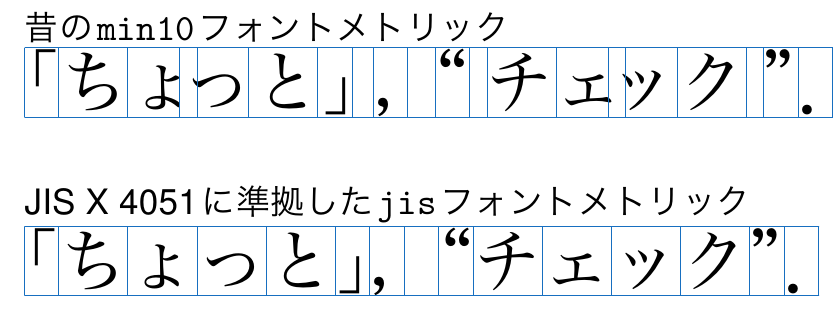
\includegraphics[width=.4\linewidth]{./image2012-gum/Okumura2011.png}
  \caption{$BF|K\8lAHHG$NNc!#>e$,(B{\pLaTeX}$B$rMQ$$$?>l9g!#2<$,1|B<$5$s$N?7%I%-%e%a%s%H%/%i%9$rMQ$$$?>l9g(B($B1|B<(B, 2011)$B!#(B}
  \label{fig:jisx0451}
  \vspace{-1em}
\end{figure}
$B6gFIE@$d3g8L$N=hM}$,:Y$+$/D4@0$5$l$F$$$kMM;R$,8+$F$H$l$^$9!#(B

$B:G8e$K(B Unicode $BBP1~$K$D$$$F!#(B
$B@h$:$*CG$j$H$7$F!"(B{\TeX}$B$K$*$1$kB?8@8l=hM}$K$D$$$F$O$3$3$G$O3d0&$7$^$9(B\footnote{
  $B6=L#$N$"$kJ}$O0J2<$N(B URL $B$r;2>H$7$F2<$5$$(B\\
  $B!V(BpTeX$B$HB?8@8l=hM}!W(B{\tt{\url{http://oku.edu.mie-u.ac.jp/~okumura/texwiki/?pTeX\%E3\%81\%A8\%E5\%A4\%9A\%E8\%A8\%80\%E8\%AA\%9E\%E5\%87\%A6\%E7\%90\%86}}}
}$B!#(B
%
$B!V%U%!%$%k$NJ8;z%3!<%I$H$7$F(B UTF-8 $B$r;H$$$?$$!W$D$^$j!VB?8@8l:.:_$N(B UTF-8 $B$N%U%!%$%k$rD>@\=hM}$7$?$$!W$H$$$&(B
$B>l9g$K$b!":G?7$N(B{\pLaTeX}($B@53N$K$O(B $\varepsilon-$$B3HD%$,$J$5$l$?(B $\varepsilon-$\pTeX)$B$G$"$l$P!"(B
$B$=$N$^$^=hM}$G$-$^$9!#$D$^$j!"<!$N0BDjHG(B(Wheezy)$B$G$O!"(BUTF-8 $B$GJ]B8$5$l$?%=!<%9$r$=$N$^$^(B \pLaTeX $B$G=hM}$G$-$k$h$&$K$J$k!D!D$O$:$G$9(B%
($B;DG0$J$,$i(B squeeze $B$G$O=hM}$G$-$^$;$s(B)$B!#(B

\subsubsection{$B@$3&>p@*(B}

$B$3$3$G0lC<F|K\8l$rN%$l$F!"(B
$BF|K\8l0J30$N(B{\TeX}($B$H$=$N3HD%(B)$B$*$h$SB?8@8l=hM}$,$I$NMM$KH/E8$7$F$$$k$N$+!"$K$D$$$F4JC1$K?($l$F$_$^$7$g$&!#(B
%
Knuth$B$5$s$N(B{\TeX}$B3+H/=*N;@k8@$N8e$G$b!"(B
$B:G2<AX$N=hM}7O$H$7$F$N(B{\TeX}$B$O?J2=$rB3$1$F$*$j!"(B$\varepsilon-$\TeX$B!"$=$7$F(B pdf\TeX $B$X$H?JE8$7$F$$$^$9!#(B
$B8=:_$G$O(B{\LaTeX}$B$H$7$F(B{pdf\LaTeX}$B$,;H$o$l$k$N$,0lHLE*$G$9(B
% \footnote{%%
%   $B$*<j85$N4D6-$G(B{\tt{latex}}$B$HBG$C$F$_$F2<$5$$!#$*$=$i$/%(%s%8%s$H$7$F(B{\tt{pdftex}}$B$,5/F0$9$k$G$7$g$&!#(B
% }
$B!#(B
pdf{\TeX}$B$O$=$NL>$NDL$j(B DVI $B%U%!%$%k$r7P$:$KD>@\(B PDF $B%U%!%$%k$r=PNO$9$k(B{\TeX}$B%(%s%8%s$G$9!#(B
$B$3$N7k2L$H$7$F!":#8e$O(B DVI $B%U%!%$%k$O2a5n$N0dJ*$K$J$C$F$$$/$N$+$b$7$l$^$;$s(B
\footnote{
  $B$3$l$OF|K\8l=hM}$H$7$F$O$"$k0UL#$"$j$,$?$$OC$G$9!#(B
  DVI$B%U%!%$%k$K$O%U%)%s%H$N!V;2>H!W$7$+I=$l$J$$$?$a!"I=<($,4D6-$K$h$C$F0[$J$j!"(BDeVice Independent $B$,<B8=$5$l$^$;$s!#(B
  PDF $B$N>l9g$O$I$&$+!"$H$$$($P!"$=$b$=$b2$J8$N(BPDF$B$N>l9g$K$O%U%)%s%H$rKd$a9~$`$N$,0lHLE*$G$"$j!"(B
  $BOBJ8$N$_$,;2>HL>(B({\tt{Ryumin-Light, GothicBBB-Medium}})$B$N$_$G<B%U%)%s%H$OKd$a9~$^$J$$!"$H$$$&>u67$G$7$?!#(B
  $B$7$+$7$J$,$i!"(B
  JIS2004$BA08e$GF1$8%3!<%I%]%$%s%H$KJL$N%0%j%U$,3d$jEv$F$i$l$F$$$k$?$a!"(B
  $B%U%)%s%H$rKd$a9~$s$G$$$J$$(B PDF $B$G$OI=<($,0[$J$k!"$H$$$&LdBj$,H/@8$7$^$9!#(B
  %
  $B:#8e$O2$J8OBJ86hJL$J$/!"%U%)%s%H$rKd$a9~$s$@(B PDF $B$r=PNO$9$k!"$H$$$&$N$,0lHLE*$K$J$k$G$7$g$&!#(B
}
$B!#(B
$B$^$?!"(B$\varepsilon-$\TeX $B$O85!9$N(B \TeX $B$KBP$7$FB?$/$N3HD%$,$J$5$l$F$$$^$9!#(B
$B8=:_4{$KB?$/$N3HD%5!G=$,(B$\varepsilon-${\TeX}$B$K0MB8$7$F$$$k$?$a!"(B
$\varepsilon-${\TeX}$B$KBP1~$7$F$$$J$$%(%s%8%s$O;~BeCY$l$K$J$j$+$M$^$;$s(B%
\footnote{%
  $B9,$$$J;v$KKL@n90E5$5$s$rCf?4$K(B$\varepsilon-$\pTeX(=\pTeX + $\varepsilon-$TeX)$B$,8x3+$5$l$F$*$j!"(B
  TeXLive $BK\BN$K$bF1:-$5$l$F$$$^$9!#K\869F<9I.;~E@$G$O4{$K(B
  Debian unstable $B$GF|K\8l4D6-$rF3F~$9$k$H(B \pLaTeX $B$N%(%s%8%s$H$7$F(B $\varepsilon-$\pTeX $B$,;H$o$l$F$$$^$9!#(B
}

$BB?8@8l=hM}7O$H$7$F$O!"ATBg$J;n$_$G$"$C$?(B$\Omega$$B$,F\:C(B(?)$B$7$?8e!"(B
$B8=:_$G$O(BXeTeX(=$\varepsilon-$\TeX + Unicode + OpenType) $B$rMQ$$$k$N$,0lHLE*$K$J$C$F$-$^$7$?!#(B
Unicode $B$G$NF~=PNO$r=hM}$7!"%7%9%F%`$N%U%)%s%H$rMxMQ$7$FD>@\(B PDF $B$r=PNO$7$^$9!#(B
%
$B$^$?!"(Bpdf{\TeX}$B$N8e7Q$H$7$F(BLua{\TeX}(pdf\TeX + $\Omega$ + Lua + METAPOST + OpenType)$B$N3+H/$,?J$a$i$l$F$$$^$9!#(B
Lua $B$K$h$k=@Fp$J3HD%$,2DG=$H$J$C$F$*$j!":#8e$N?JE8$,3Z$7$_$G$O$"$j$^$9!#(B

$B$J$*!"8=;~E@$G$O(B Xe(La)TeX $B$*$h$S(B LuaTeX $B$rMQ$$$F!"(B
JIS X 4051 $B$G5,Dj$5$l$?F|K\8l$NAHHG$r<B8=$9$k$?$a$K$OJL%Q%C%1!<%8$,I,MW$@$C$?$j!"(B
$B%W%j%"%s%V%k$r$=$l$J$j$K=$@5$9$kI,MW$,$"$k$N$G0l6ZFl$G$O$$$-$^$;$s!#(B
%
$B:#8e$KHw$($FF08~$r3NG'$7$F$*$/$N$bNI$$$G$7$g$&(B
\footnote{
  \noindent
  XeTeX $B$K4X$7$F$O!V(BXeLaTeX$B$GF|K\8l$9$k7o$K$D$$$F!W(B{\tt{\url{http://zrbabbler.sp.land.to/xelatex.html}}} \\
  LuaTeX-ja $B$K4X$7$F$O!V(BLuaTeX-ja $B%W%m%8%'%/%H!W(B{\tt{\url{http://sourceforge.jp/projects/luatex-ja/wiki/FrontPage}}}
}$B!#(B

\subsubsection{{\TeX}Live $B$K$D$$$F(B}

$B:G8e$K!"(B{\TeX}Live$B$K$D$$$F!#(B
{\TeX}$B$K4X$9$k%=%U%H%&%'%"$rDs6!$9$k!V%G%#%9%H%j%S%e!<%7%g%s!W$H$7$F!"0JA0$O(B te\TeX $B$,%j%j!<%9$5$l$F$$$^$7$?!#(B
$B$7$+$7$J$,$i!"(B2009$BG/$K(B te\TeX $B$H$7$F%j%j!<%9$rDd;_$7$?8e(B\footnote{%
   teTeX: no next release
   $B!V(B{\tt{\url{http://article.gmane.org/gmane.comp.tex.tetex.beta/812}}}$B!W(B
}$B!"(B
{\TeX}Live $B$,(B{\TeX}$B$N%G%#%9%H%j%S%e!<%7%g%s$H$7$F%j%j!<%9$5$l$k$h$&$K$J$j$^$7$?!#(B
%
{\TeX}Live $B$N%j%j!<%9%^%M!<%8%c$O(B Norbert Preining $B$5$s$G!"(B
$BH`$O(B Debian $B$N(B {\TeX} $B4XO"%Q%C%1!<%8$N%a%s%F%J$G$b$"$j$^$9!#(B
{\TeX}Live $B$G$O(B {\tt{tpm2deb}} $B$d(B {\tt{tpm2rpm}} $B$H$$$C$?%Q%C%1!<%8JQ49%9%/%j%W%H$bDs6!$5$l$F$*$j!"(B
$B8=:_$G$OB?$/$N(B Linux $B%G%#%9%H%j%S%e!<%?$,(B {\TeX}Live $B$r85$K3F!9$N%Q%C%1!<%8$r:n@.$7$F$$$^$9!#(B
%
$BF|K\8l4XO"$K$D$$$F$O!"(B2010$BG/0J9_$K(B {\TeX}Live$BK\BN$X$N(B \pTeX$B!"(Bj{\TeX} $B$N%^!<%8$,3+;O$5$l!"(B
$BK\869F<9I.;~E@$G$O!"(Bpatch $B$NCx:n8"<T$K%3%s%?%/%H$N<h$l$F$$$J$$(B {\tt{xdvik-ja}} $B0J30$O(B
$B$[$\%^!<%8$,40N;$7$F$$$^$9!#(B

\subsection{Debian$B$K$*$1$k(B($BF|K\8l(B){\TeX}$B4D6-(B}

$B$5$F$3$3$^$G$N$*OC$rF'$^$($?>e$G!"$h$&$d$/(B Debian $B$N(B{\TeX}$B4D6-$K$D$$$F?($l$F$$$-$^$9!#(B
%
$B$A$J$_$K!"!V(BDebian$B$G$N(B{\pLaTeX}$B$N@_Dj!W$_$?$$$JOC$O$0$0$k$H7k9=$G$F$/$k$N$G!"$"$^$j?($l$^$;$s(B
\footnote{%
  $BH/I=;~$*$h$SH/I=8e$O(B Q\&A $B$*$h$S@_Dj$N$*<jEA$$$O9T$J$$$^$9!#(B
}$B!#(B

\subsubsection{Squeeze $B$K$*$1$k(B($BF|K\8l(B){\TeX}$B4D6-(B}

Squeeze $B$K$FG[I[$5$l$F$$$k(B {\TeX}Live $B$N%P!<%8%g%s$O(B 2009 $B$G$9!#(B
$B$G$9$N$G(B \pTeX $B$*$h$S(B j{\TeX} $B4XO"$O!"(B
$\varepsilon-$\TeX $B3HD%A0$N(B{\bf{UTF-8}}
$B$N%U%!%$%k$r=hM}$G$-$J$$%P!<%8%g%s$G$9!#(B
$B6qBNE*$K$O!"(B{\tt{ptex-buildsupport}} $B%Q%C%1!<%8$G(B te{\TeX}$B$N%=!<%9$rDs6!$7!"(B
$B$3$l$K(B patch $B$rEv$F$k$3$H$G(B \pTeX $B$d(B j{\TeX} $B$N%Q%C%1!<%8$,9=C[$5$l$F$$$^$9!#(B
%
$B$^$?!"%Y!<%9$H$J$C$F$$$k(Bte{\TeX}$B$N%P!<%8%g%s$b(B 2007 $B$G$"$j!"(B
$B%;%-%e%j%F%#%U%#%C%/%9$O$J$5$l$F$$$k$b$N$N!"(B
$BBg;(GD$K8@$($P(B{\bf{2007$BG/$+$i99?7$5$l$F$$$^$;$s(B}}\footnote{%
  Squeeze $B%j%j!<%9A0$K(B xdvik-ja $B$N(B 64bit $BBP1~$NI,MW$,$"$j!"(B
  $B:4!9LZ$,(B patch $B$rEv$F$F%Q%C%1!<%8$r:F9=C[$7$?$j$7$^$7$?!#(B
}$B!#(B

$BF3F~8e$K$b!"(B
DVI $B%U%!%$%k$NI=<($d(B PostScript/PDF $B$X$NJQ49$N$?$a$K(B
$B4v$D$+$*$^$8$J$$$,I,MW$@$C$?$j$7$^$9!#(B
%
$BNc$($P(B
\begin{enumerate}
\item dvipsk-ja $BMQ$N(B VF $B%U%!%$%k$N=`Hw$N$?$a$K!"%$%s%9%H!<%k8e$K0J2<$r>'$($k!#(B
  \begin{commandline}
    $ sudo jisftconfig add
  \end{commandline}
  % $
\item xdvik-ja $B$G$NI=<($N$?$a$K(B
  \begin{commandline}
    # $BL@D+7O$NI=<($K;HMQ$9$k%U%)%s%H(B
    $ fc-match serif:lang=ja
    # $B%4%7%C%/7O$NI=<($K;HMQ$9$k%U%)%s%H(B
    $ fc-match sans-serif:lang=ja
  \end{commandline}
  \noindent $B$r3NG'$7(B
  % \footnote{%
  %   {\tt{ttf-tamil-fonts}} $B$d(B
  %   {\tt{ttf-devanagari-fonts}} $B$,%$%s%9%H!<%k$5$l$F$$$k>l9g$K$O!"(B
  %   $B$3$l$i$,JV$C$F$-$F$7$^$$!"(B
  %   $B7k2L$H$7$F(B DVI $B$NI=<($K$3$l$i$N%U%)%s%H$,;H$o$l$k!#(B
  % }
  $B!"(B
  $BI,MW$K1~$8$F!"(B{\tt{$\tilde{}$/.fonts.conf}} $B$K(B
  {\tt{serif, sans-serif}}$B$N%(%s%H%j$rDI5-$7$F(B
  \begin{commandline}
    $ sudo update-vfontmap
  \end{commandline}
  % $
\item $B%U%)%s%H$,Kd$a9~$^$l$F$$$J$$(B
  PDF $B$NI=<($N$?$a$K!"(B{\tt{Ryumin, Gothic-BBB}}$B$N%(%s%H%j$r(B
  {\tt{$\tilde{}$/.fonts.conf}}$B$KDI5-$9$k!#(B
\item $B%U%)%s%H$rKd$a9~$s$@(B PDF $B$r@8@.$9$k$?$a$K$O!"(B
  {\tt{/etc/texmf/texmf.d/75DviPS.cnf}} $B$N(B {\tt{TTFONTS}}$B!"(B
  $B$b$7$/$O(B{\tt{\%OSFONTDIR}} $B$KKd$a9~$_$?$$%U%)%s%H$N%Q%9$rDI2C$7$?8e$K(B
  \begin{commandline}
    $ sudo update-texmf
  \end{commandline}
  % $
  $B$r>'$($F!"$5$i$K(B map $B%U%!%$%k$rE,Ev$KMQ0U$7$F$*$/!#(B
\end{enumerate}
\vspace{-.8em}
$B$J$I$G$9!#(B

\subsubsection{Squeeze$B$G(B{\tt{{\TeX}Live(>=2011)}}$B$r;H$&(B!?}

Debian$B$N%Q%C%1!<%8$G$O$"$j$^$;$s$,!"(Bamd64 $B$b$7$/$O(B i386 $B$N>l9g$K$O(B
Norbert $B$5$s$rCf?4$KDs6!$5$l$F$$$k!V(Btlptexlive $B%j%]%8%H%j(B\footnote{
  tlptexlive $B%j%]%8%H%j!V(B{\tt{\url{http://tutimura.ath.cx/ptexlive/?tlptexlive\%A5\%EA\%A5\%DD\%A5\%B8\%A5\%C8\%A5\%EA}}}$B!W(B
}$B!W$+$i!"(B
TeXLive $BA4BN$N%3%s%Q%$%k:Q$_%P%$%J%j$r<hF@$7$F;HMQ$9$k!"$H$$$&J}K!$b$"$j$^$9!#(B
%
$B$3$N>l9g$K$O(B
\begin{enumerate}
\item $B4{B8$N(B Debian $B%Q%C%1!<%8$N0MB84X782r>C$N$?$a$K(B {\tt{equivs}} $B$G%@%_!<%Q%C%1!<%8$r:n@.$9$k(B
\item {\TeX}Live $B$N%Q%C%1!<%8%^%M!<%8%c$G$"$k(B{\tt{tlmpgr}}$B$G$N%P%$%J%jF3F~@h$r!"(B
  $B4IM}$7$d$9$$=j$KDI$$$F$*$/!#(B
\end{enumerate}
$B$J$s$F9)IW$,I,MW$G$7$g$&!#:4!9LZ$O(B Squeeze $B4D6-$G(B
$B$O(B {\tt{stow}} $B$G(B tlptexlive $B%j%]%8%H%j$G$N%$%s%9%H!<%kJ*$r4IM}$7$F$$$^$9!#(B

$B$A$J$_$K(B tlptexlive $B$NG[I[J*$O(B {\tt{{\TeX}Live (>= 2011)}} $BAjEv$G$9$N$G!"(B
$B%U%)%s%H<~$j$N@_Dj$O8e=R$N(B Wheezy $B$N>l9g$HF1$8$G$9!#(B

\subsubsection{Wheezy $B$N8=>u(B}

$B4{$K(B{\TeX}Live 2011(2012/dev) $B$,(B Sid $B$K(B upload $B$5$l$F$$$^$9!#$7$+$7$J$,$i!"(B
$BK\869F<9I.;~E@$G$O$^$@(B Wheezy $B$K$O99?7$5$l$?(B{\TeX}$B4XO"$N%Q%C%1!<%8$OMn$A(B
$B$F$-$F$$$^$;$s!#(B
$BH/I=;~$K$O(B Wheezy $B$KMn$A$F$-$F$$$k$3$H$r4|BT$7$D$D!"(B
$BJQ99E@$r4JC1$K=R$Y$F$_$^$9!#(B

$B$3$N%P!<%8%g%s$N(B {\TeX}Live $B$K$O4{$K(B\pTeX $B$J$I$,%^!<%8$5$l$F$$$k$?$a!"(B
Squeeze $B$^$G$GDs6!$7$F$$$?(B te\TeX $B%Y!<%9$N%Q%C%1!<%872(B{\tt{ptex-bin, ptex-base, ...}}$B$O8.JB(B obsolete $B$H$J$j$^$9(B\footnote{%
  {\TeX}Live $BK\BN$K%^!<%8$5$l$F$$$J$$(B{\tt{xdvik-ja}}$B$N$_$,;D$k$3$H$K$J$j$^$9!#(B
}$B!#(B
%
$B8=>u$G$O(B \pTeX $B4XO"$O(B {\tt{texlive-binaries, texlive-lang-cjk}} $B$rF3F~$9$k$3$H$G0l3g$G(B install $B$5$l$kM=Dj$G$9!#(B
$B$^$?!"%U%)%s%H4XO"$N07$$$b(B {\tt{updmap-setup-kanji}} $B$H$$$&%3%^%s%I$K$h$C$F!"0l3g$G@_Dj$G$-$k$h$&$K$J$j$^$9!#(B
%
$B$?$H$($P(B
\begin{commandline}
  $ sudo updmap-setup-kanji nofont
\end{commandline}
%$
\noindent $B$H$$$C$?1vG_$G$9(B($B>e5-$N@_Dj$O!"%U%)%s%H$r$^$C$?$/Kd$a9~$^$J$$>l9g$G$9(B)$B!#(B
$B$3$N%3%^%s%I$K$h$j!"(B{\tt{xdvik-ja, dvips, dvipdfmx}} $B$N%U%)%s%H%^%C%W$,0l3g$7$F99?7$5$l$^$9!#(B
%
{\TeX}Live $B$G$O%U%)%s%H%^%C%W%U%!%$%k$H$7$F!"(B
1)$BKd$a9~$^$J$$>l9g!"(B 2)IPAex $B$r;H$&>l9g!"(B3)$B%R%i%.%N$r;H$&>l9g!"(B4)$B>.DM%U%)%s%H$r;H$&>l9g(B
$B$N(B 4 $B$D$rDs6!$7$F$*$j!"(BDebian $B$N%Q%C%1!<%8$G$b$3$l$i$N%^%C%W%U%!%$%k$rDs6!$7$F$$$^$9!#(B
Debian $B$N(B main $B%;%/%7%g%s$N$_$G:n6H$r$9$k>l9g$K$O(B 1) or 2) $B$r;H$&$3$H$K$J$k$G$7$g$&!#(B
$B8=;~E@$G$O!"(B
\begin{itemize}
\item Conflicts, Replace, Provides $B$N@_Dj$,H>C<$G(B
  Squeeze $B$+$i$N(B upgrade $B$,$&$^$/$G$-$J$$(B($B%Q%C%1!<%8$,$"$k(B)$B!#(B
\item {\TeX}Live $BK\BN$G$bG[I[$5$l$F$$$k%U%)%s%H$,$"$j!"(B
  $B4{B8$N%Q%C%1!<%8$H=EJ#$7$F$$$k$?$a!"(BDepends $B$rDI2C$7$FE,59(B symbolic link $B$K(B
  $BCV49$9$kI,MW$,$"$k!#(B
\end{itemize}
$B$H$$$C$?LdBj$,$"$C$F!":#8e$N=$@5$,BgJQ$G$9$,!"(B
Wheezy $B$N%j%j!<%9$^$G$K$O$A$c$s$HD>$k(B($BD>$9(B?)$B$G$7$g$&!#(B

\subsection{$B:G8e$K(B}

$B6n$1B-$G$7$?$,!"F|K\8l(B{\TeX}$B$N8=>u$*$h$S(B
Debian $B$G$N(B{\TeX}$B4XO"$N8=>u$r$^$H$a$F$_$^$7$?!#(B
%
$B$^$@$^$@=$@5$9$Y$-E@$b$"$j$^$9$,!"(B
$B:#8e$O(B{\tt{updmap-setup-kanji}}$B$K$h$k%U%)%s%H4XO"$N0l3g4IM}$,M-8z$K$J$k$?$a!"(B
$B$*$^$8$J$$$N$h$&$J!"(B
$B$H$b$9$l$P%P%C%I%N%&%O%&$H07$o$l$,$A$JHQ;($J@_Dj$OITMW$K$J$k$G$7$g$&!#(B
%
Wheezy $B$+$i$O!"(BUTF-8 $B$XBP1~$7$?(B \pTeX $B$,!"(B
$B$b$C$H8@$($P(BJIX X 4051$B$NAHHGMW7o$rK~$?$7$D$DB?8@8l=hM}$b2DG=$H$J$C$?(B
$BF|K\8l(B{\TeX}$B4D6-$,Hs>o$K4JC1$K<j$KF~$k$h$&$K$J$kM=Dj$G$9(B\footnote{%
  $BK\Mh$G$"$l$P$3$3$G;29MJ88%$rNs5-$9$Y$-$G$9$,!"(B
  $B;fLL$NET9g>e5SCm$K5-$9L5:nK!$r$*5v$72<$5$$!#(B
}$B!#(B



%------------------------------------------------------------------------------
\dancersection{Linux-PAM$B$N@_Dj$K$D$$$F(B}{$B@>;3OB9-(B}
\label{linux-pam}
\subsection{Introduction}
\label{sec-1-1}
\subsubsection{PAM $B$H$O2?$+(B?}
\label{sec-1-1-1}
%------------------------------------------------------------------------------

Linux-PAM (Pluggable Authentication Modules for Linux) $B$H$O!"%"%W%j%1!<%7%g%s$,%f!<%6!<$r$I$&G'>Z$9$k$+$r%m!<%+%k%7%9%F%`$N4IM}<T$,@_Dj$G$-$k$h$&$K$9$k$?$a$N6&M-%i%$%V%i%j0l<0$G$9!#(B

PAM $B$N$*$+$2$G!"%"%W%j%1!<%7%g%s$r%3%s%Q%$%k$7$J$*$5$J$/$F$b!"G'>ZJ}K!$rJQ99$7$?$j!"8"8B$NIUM?$N;EJ}$rJQ99$7$?$j$G$-$k$h$&$K$J$C$F$$$^$9!#(B
\subsubsection{NSS $B$H$O2?$+(B?}
\label{sec-1-1-2}

PAM $B$H4X78$N?<$$%i%$%V%i%j$H$7$F(B NSS (Name Service Switch) $B$,$"$j$^$9!#(B
NSS $B$O%f!<%6!<L>$H%f!<%6!<(B ID $B$H$NJQ49$r$7$?$j!"%[%9%HL>$H(B IP $B%"%I%l%9$H$NJQ49$r$7$?$j$9$k$H$-$K;H$o$l$^$9!#(B
\subsubsection{PAM $B$H(B NSS $B$H$N0c$$(B}
\label{sec-1-1-3}

PAM $B$OG'>ZItJ,$N$_$J$N$G!"4pK\E*$K$O%m%0%$%s$d%m%0%"%&%H$N$H$-$H%Q%9%o!<%IJQ99$K4X78$7$^$9!#(B ($B87L)$K$O%"%W%j%1!<%7%g%s<!Bh$G$9!#(B)

$B%m%0%$%sCf$K(B \verb~id~ $B%3%^%s%I$GI=<($5$l$k%f!<%6!<(BID$B$H%f!<%6!<L>$NBP1~(B \footnote{$B%0%k!<%W(BID$B$H%0%k!<%WL>$bF1MM$G$9!#(B } $B$d(B \verb~ls -l~ $B$G%U%!%$%k%7%9%F%`$K5-O?$5$l$F$$$k%f!<%6!<(BID$B$+$i%f!<%6!<L>$X$NJQ49(B \footnote{$B%U%!%$%k%7%9%F%`$K$O=jM-<T$O%f!<%6!<(BID$B$G5-O?$5$l$F$$$^$9!#$=$N$?$a!"$?$H$($P%f!<%6!<$r:o=|$7$FB8:_$7$J$$%f!<%6!<$N%U%!%$%k$,$"$k>l9g$K$O!"%f!<%6!<L>$X$NJQ49$,=PMh$J$$$N$G?t;z$GI=<($5$l$^$9!#(B } $B$J$I$O(B \verb~/etc/nsswitch.conf~ $B$G@_Dj$9$k(B NSS $B$N5!G=$K$J$j$^$9!#(B
\subsubsection{PAM $B$N@_Dj(B}
\label{sec-1-1-4}

PAM $B$O@_Dj%U%!%$%k$K<B9T$7$?$$%b%8%e!<%k$rJB$Y$F$*$$$F!"$=$l$r=gHV$K<B9T$7$F$$$/$h$&$J$b$N$@$H;W$($PNI$$$G$7$g$&!#(B

$B$?$H$($P!"(B
\begin{itemize}
\item \verb~/etc/passwd~ $B$J$I$N%m!<%+%k%U%!%$%k$G$NG'>Z(B
\begin{itemize}
\item $B@.8y$9$l$PG'>Z@.8y$r%"%W%j%1!<%7%g%s$KJV$9(B
\item $B<:GT$9$l$P<!$X(B
\end{itemize}
\item LDAP $B$G$NG'>Z(B
\begin{itemize}
\item $B@.8y$9$l$PG'>Z@.8y$r%"%W%j%1!<%7%g%s$KJV$9(B
\item $B<:GT$9$l$P<!$X(B
\end{itemize}
\item $B<!$,$J$$$N$GG'>Z<:GT$r%"%W%j%1!<%7%g%s$KJV$9(B
\end{itemize}
$B$H$$$&F0:n$r$7$^$9!#(B
\subsection{$B%U%!%$%kG[CV(B}
\label{sec-1-2}
\subsubsection{$B@_Dj%U%!%$%k(B}
\label{sec-1-2-1}

\verb~/etc/pam.d/~ $B$N2<$K%"%W%j%1!<%7%g%s$4$H$N@_Dj%U%!%$%k$,$"$j$^$9!#(B
$B0J2<$O$=$NNc$G$9!#(B


\begin{commandline}
$ ls /etc/pam.d
atd       chsh            common-password                cron      other   su
chfn      common-account  common-session                 login     passwd  sudo
chpasswd  common-auth     common-session-noninteractive  newusers  sshd
\end{commandline}
%$

\begin{itemize}
\item $B$I$N@_Dj%U%!%$%k$,$I$N%"%W%j%1!<%7%g%s$N$b$N$J$N$+$O%U%!%$%kL>$+$i?dB,$G$-$^$9(B
\item $B$J$$>l9g$O(B \verb~other~ $B$,;H$o$l$^$9(B
\item $B$=$l$>$l$NCf$+$i(B \verb~@include~ $B$G(B \verb~common-*~ $B$G6&DL$N@_Dj$r;H$&$h$&$K$J$C$F$$$^$9(B
\end{itemize}

\verb~/etc/pam.d/~ $B$,$J$$>l9g$O(B \verb~/etc/pam.conf~ $B$,;H$o$l$k$H(B \verb~/etc/pam.conf~ $B$NCf$N%3%a%s%H$K=q$$$F$"$j$^$9$,!"$3$N5-=R$ONr;KE*$J$b$N$G:G6a$N(B Linux $B$G$O;H$o$l$F$$$^$;$s!#(B
\subsubsection{$B%b%8%e!<%k(B}
\label{sec-1-2-2}

$B0J2<$O(B PAM $B%b%8%e!<%k$NNc$G$9!#(B


\begin{commandline}
$ ls /lib/x86_64-linux-gnu/security
pam_access.so     pam_keyinit.so    pam_nologin.so     pam_tally.so
pam_debug.so      pam_lastlog.so    pam_permit.so      pam_tally2.so
pam_deny.so       pam_ldap.so       pam_pwhistory.so   pam_time.so
pam_echo.so       pam_limits.so     pam_rhosts.so      pam_timestamp.so
pam_env.so        pam_listfile.so   pam_rootok.so      pam_umask.so
pam_exec.so       pam_localuser.so  pam_securetty.so   pam_unix.so
pam_faildelay.so  pam_loginuid.so   pam_selinux.so     pam_userdb.so
pam_filter.so     pam_mail.so       pam_sepermit.so    pam_warn.so
pam_ftp.so        pam_mkhomedir.so  pam_shells.so      pam_wheel.so
pam_group.so      pam_motd.so       pam_stress.so      pam_xauth.so
pam_issue.so      pam_namespace.so  pam_succeed_if.so
\end{commandline}
%$

\begin{itemize}
\item $B@_Dj%U%!%$%k$K=q$+$l$k(B \verb~pam_unix.so~ $B$J$I$O(B \verb~dlopen(3)~ $B$GF0E*$KFI$_9~$^$l$^$9(B
\item $B$=$N$?$a(B PAM $B$NG'>Z$r;H$C$F$$$k%W%m%0%i%`$rF~$l$?(B chroot $B4D6-$r:n$k$H$-$K$O5$$r$D$1$kI,MW$,$"$j$^$9(B
\item \verb~squeeze~ $B$^$G$O(B \verb~/lib/security/~ $B$d(B \verb~/lib64/security/~ $B$K$"$j$^$9(B
\item \verb~multiarch~ $BBP1~$G:G6a$O(B \verb~/lib/x86_64-linux-gnu/security/~ $B$J$I$N(B \verb~/lib/<triplet>/security/~ $B$K$"$j$^$9!#(B
  $B>e5-$NNc$O(B wheezy (testing) $B$J$N$G(B \verb~/lib/security/~ $B$G$O$J$/(B
  \verb~/lib/x86_64-linux-gnu/security/~ $B$K$J$C$F$$$^$9(B
\end{itemize}
\subsection{$B@_Dj%U%!%$%k$N=q<0(B}
\label{sec-1-3}

$B@_Dj%U%!%$%k$NNc$r:\$;$F$*$-$^$9!#(B($B0lIt>JN,(B)

\begin{commandline}
$ egrep '^[^#]' /etc/pam.d/cron
@include common-auth
session       required   pam_env.so
session       required   pam_env.so envfile=/etc/default/locale
@include common-account
@include common-session-noninteractive
session    required   pam_limits.so
\end{commandline}
%$

\begin{itemize}
\item $B@_Dj%U%!%$%k$K$O0J2<$N9`L\$r;XDj$7$^$9!#>\:Y$O8e=R$7$^$9(B
\begin{description}
\item[\verb~service~] $B%"%W%j%1!<%7%g%s$KBP1~$9$kL>A0(B
\item[\verb~type~] PAM $B$NJ,N`(B
\item[\verb~control~] $BF0:n;XDj(B
\item[\verb~modules-path~] PAM $B%b%8%e!<%k$X$N%Q%9(B
\item[\verb~module-arguments~] PAM $B%b%8%e!<%k$N0z?t(B
\end{description}
\item \verb~#~ $B$+$i9TKv$^$G$O%3%a%s%H$K$J$j$^$9(B
\item \verb~\~ $B$,2~9T(B (\verb~<LF>~) $B$ND>A0$K$"$k$H7QB39T$K$J$j$^$9(B
\item \verb~/etc/pam.conf~ $B$G$O!V(B \verb~service type control module-path module-arguments~ $B!W$H$$$&=q<0$G@_Dj$7$^$9!#(B( \verb~service~, \verb~type~, \verb~control~ $B$NBgJ8;z>.J8;z$OL5;k$5$l$^$9!#(B)
\item \verb~/etc/pam.d/~ $B$G$O(B \verb~service~ $B$,%U%!%$%kL>(B ($BI,$:>.J8;z(B) $B$K$J$j$^$9(B
\item $B;D$j$N!V(B \verb~type control module-path module-arguments~ $B!W$,%U%!%$%k$NFbMF$K$J$j$^$9(B
\end{itemize}
\subsubsection{service}
\label{sec-1-3-1}

\begin{itemize}
\item \verb~service~ $B$O6qBNE*$K$O(B \verb~login~ $B$d(B \verb~su~ $B$K$J$j$^$9(B
\item \verb~other~ $B$H$$$&(B \verb~service~ $BL>$O%G%U%)%k%H@_DjMQ$H$7$FM=Ls$5$l$F$$$^$9(B
\item Debian $B$G$O(B \verb~common-~ $B$G;O$^$kL>A0$N%U%!%$%k$,6&DL@_DjMQ$N%U%!%$%k$K$J$C$F$$$F!"B>$N@_Dj%U%!%$%k$+$i(B \verb~@include~ $B$GFI$_9~$^$l$F$$$^$9(B
\end{itemize}
\subsubsection{type}
\label{sec-1-3-2}

\begin{description}
\item[account] $BG'>Z0J30$N%"%+%&%s%H4IM}$K;H$o$l$^$9!#$?$H$($PCk4V$@$1%m%0%$%s$G$-$k$h$&$K$7$?$j!"(B \verb~nologin~ $B%U%!%$%k$,$"$k$H$-$O0lHL%f!<%6!<$K%m%0%$%s$5$;$J$$$h$&$K$7$?$j$G$-$^$9(B
\item[auth] $B%"%W%j%1!<%7%g%s$K%Q%9%o!<%IF~NO$rMW5a$9$k$J$I$NJ}K!$G%f!<%6!<G'>Z$r$7$^$9!#%0%k!<%W8"8B$NIUM?$J$I$N5!G=$b$"$j$^$9(B
\item[password] $B%Q%9%o!<%IJQ99$J$I$NG'>Z%H!<%/%sJQ995!G=$rDs6!$7$^$9(B
\item[session] $B%5!<%S%9MxMQ$NA08e$K2?$+$r$9$k%b%8%e!<%k%?%$%W$G$9!#%m%0$r<h$C$?$j!"%G%#%l%/%H%j$r%^%&%s%H$7$?$j!"(B \verb~/etc/motd~ $B$rI=<($7$?$j!"4D6-JQ?t$r@_Dj$7$?$j$G$-$^$9(B
\item[\verb~@include~] Debian $B$G$O$3$3$K(B \verb~@include~ $B$r;XDj$9$k$3$H$GJL$N%U%!%$%k$rFI$_9~$a$k$h$&$K$J$C$F$$$^$9(B
\end{description}
\subsubsection{control}
\label{sec-1-3-3}

PAM $B%b%8%e!<%k$r<B9T$7$F$=$N7k2L!"$I$&$9$k$N$+$N@_Dj$G$9!#(B
$B>\:Y$K$D$$$F$O8e=R$7$^$9!#(B
\subsubsection{module-path}
\label{sec-1-3-4}

PAM $B%b%8%e!<%k$N%U%!%$%k$X$N%Q%9$r@dBP%Q%9$+%G%U%)%k%H$N%b%8%e!<%k$NCV$->l=j$G$"$k(B \verb~/lib/security/~ $B$J$I$+$i$NAjBP%Q%9$G;XDj$7$^$9!#(B
\subsubsection{module-arguments}
\label{sec-1-3-5}

$B%9%Z!<%96h@Z$j$G%b%8%e!<%k$X$N0z?t$r;XDj$7$^$9!#(B
$B%9%Z!<%9$r4^$`0z?t$r;XDj$9$k>l9g$O0J2<$NNc$N$h$&$K(B \verb~[]~ $B$G$/$/$j$^$9!#(B


\begin{commandline}
squid auth required pam_mysql.so user=passwd_query passwd=mada \
      db=eminence [query=select user_name from internet_service \
      where user_name='%u' and password=PASSWORD('%p') and \
      service='web_proxy']
\end{commandline}

\verb~]~ $B$r4^$a$?$$>l9g$O(B \verb~\]~ $B$H;XDj$7$^$9!#(B
$B$D$^$j0J2<$N$h$&$K$J$j$^$9!#(B


\begin{commandline}
[..[..\]..]    -->   ..[..]..
\end{commandline}
\subsection{control $B$N@_Dj$K$D$$$F(B}
\label{sec-1-4}
\subsubsection{PAM $B$NFbIt>uBV(B}
\label{sec-1-4-1}

PAM $B$O%b%8%e!<%k$r<B9T$7$F$$$/$H$-$KFbItE*$K(B
\begin{itemize}
\item $B=i4|>uBV(B
\item $B@.8y>uBV(B
\item $B<:GT>uBV(B
\end{itemize}
$B$N(B3$B$D$N>uBV$,$"$j!":G=*E*$K@.8y>uBV$J$i@.8y$r%"%W%j%1!<%7%g%s$KJV$7!"$=$&$G$J$1$l$P<:GT$r%"%W%j%1!<%7%g%s$KJV$7$^$9!#(B
($B=i4|>uBV$N$^$^$N$H$-$b<:GT$rJV$7$^$9!#(B)
\subsubsection{control $B$N>JN,7A<0(B}
\label{sec-1-4-2}

control $B$N;XDj$K$O!">JN,$7$?7A<0$H$7$F0J2<$N$b$N$,$"$j$^$9!#(B

\begin{description}
\item[required] $B@.8y$7$F$b<:GT$7$F$bB3$-$r<B9T$7$F$+$i7k2L$rJV$7$^$9!#<:GT>uBV0J30$G@.8y$7$?>l9g$O@.8y>uBV$K$7$^$9!#<:GT$7$?>l9g$O<:GT>uBV$K$7$^$9(B
\item[requisite] $B<:GT$7$?>l9g$O<:GT>uBV$K$7$F!"$9$0$K%"%W%j%1!<%7%g%s$K<:GT$rJV$7$^$9!#<:GT>uBV0J30$G@.8y$7$?>l9g$O@.8y>uBV$K$7$^$9(B
\item[sufficient] $B<:GT>uBV0J30$G@.8y$7$?>l9g$O!"$9$0$K%"%W%j%1!<%7%g%s$K@.8y$rJV$7$^$9!#<:GT$OL5;k$7$FB3$-$r<B9T$7$^$9(B
\item[optional] $B@.8y$+<:GT$+$O5$$K$;$:<B9T$7$?$$%b%8%e!<%k$K;H$$$^$9!#@.8y$+<:GT$+$OB>$N%b%8%e!<%k$,$J$$$H$-$@$11F6A$7$^$9(B
\item[include, substack] $B>JN,7A<0$G$O$"$j$^$;$s$,!"$3$N$h$&$J;XDj$b=PMh$^$9!#$7$+$7(B Debian $B$G$O>e=R$N(B \verb~@include~ $B$,;H$o$l$F$$$F!"$3$l$i$OIaDL$O;H$o$l$F$$$J$$$N$H!"FbIt>uBV$N@bL@$,J#;($K$J$k$?$a>JN,$7$^$9(B
\end{description}
\subsubsection{control $B$N>JN,$7$J$$7A<0(B}
\label{sec-1-4-3}

$B$b$C$HJ#;($J7A<0$H$7$F0J2<$N$b$N$,$"$j$^$9!#(B


\begin{commandline}
[value1=action1 value2=action2 ...]
\end{commandline}
\subsubsection{control $B$N(B value}
\label{sec-1-4-4}

\verb~valueN~ $B$O(B PAM $B%b%8%e!<%k$+$i$NJVCM$G(B \verb~actionN~ $B$O$=$NJVCM$N$H$-$K$I$&$9$k$+$H$$$&@_Dj$G$9!#(B
\verb~valueN~ $B$K$O!"(B

{\scriptsize
\begin{tabular}{cc}
  \begin{minipage}[b]{0.3\textwidth}
    \begin{itemize}
    \item \verb~success~
    \item \verb~open_err~
    \item \verb~symbol_err~
    \item \verb~service_err~
    \item \verb~system_err~
    \item \verb~buf_err~
    \item \verb~perm_denied~
    \item \verb~auth_err~
    \item \verb~cred_insufficient~
    \item \verb~authinfo_unavail~
    \item \verb~user_unknown~
    \end{itemize}
  \end{minipage}
  \begin{minipage}[b]{0.3\textwidth}
    \begin{itemize}
    \item \verb~maxtries~
    \item \verb~new_authtok_reqd~
    \item \verb~acct_expired~
    \item \verb~session_err~
    \item \verb~cred_unavail~
    \item \verb~cred_expired~
    \item \verb~cred_err~
    \item \verb~no_module_data~
    \item \verb~conv_err~
    \item \verb~authtok_err~
    \item \verb~authtok_recover_err~
    \end{itemize}
  \end{minipage}
  \begin{minipage}[b]{0.3\textwidth}
    \begin{itemize}
    \item \verb~authtok_lock_busy~
    \item \verb~authtok_disable_aging~
    \item \verb~try_again~
    \item \verb~ignore~
    \item \verb~abort~
    \item \verb~authtok_expired~
    \item \verb~module_unknown~
    \item \verb~bad_item~
    \item \verb~conv_again~
    \item \verb~incomplete~
    \item \verb~default~
    \end{itemize}
  \end{minipage}
\end{tabular}
}

$B$,;XDj$G$-$^$9!#(B
\verb~default~ $B$OL>A0$+$i$o$+$kDL$jL@<(E*$K(B \verb~valueN~ $B$K;XDj$5$l$J$+$C$?$H$-$N%G%U%)%k%H;XDj$G$9!#(B

\verb~valueN~ $B$K;XDj$G$-$kCM$N40A4$J%j%9%H$O(B \verb~libpam0g-dev~ $B%Q%C%1!<%8$r%$%s%9%H!<%k$7$F(B
\begin{itemize}
\item \verb~/usr/include/security/_pam_types.h~
\end{itemize}
$B$r;2>H$7$F$/$@$5$$!#(B
\subsubsection{control $B$N(B action}
\label{sec-1-4-5}

\verb~actionN~ $B$K;XDj$G$-$k$b$N$O0J2<$NDL$j$G$9!#(B

\begin{description}
\item[ignore] $BL5;k$7$^$9!#%b%8%e!<%k$NJVCM$O%"%W%j%1!<%7%g%s$KJV$9CM$K$O1F6A$7$^$;$s(B
\item[bad] $B<:GT>uBV$K$7$^$9(B
\item[die] $B<:GT$7$^$9!#<:GT>uBV$K$7$F!"$9$0$K%"%W%j%1!<%7%g%s$K<:GT$rJV$7$^$9(B
\item[ok] $B<:GT>uBV0J30$J$i@.8y>uBV$K$7$^$9!#$9$G$K<:GT>uBV$N$H$-$O<:GT>uBV$N$^$^$G$9(B
\item[done] $B<:GT>uBV0J30$J$i@.8y>uBV$K$7$F!"$9$0$K%"%W%j%1!<%7%g%s$K@.8y$rJV$7$^$9!#$9$G$K<:GT>uBV$N$H$-$O<:GT>uBV$N$^$^$G$9(B
\item[N (1$B0J>e$N@0?t(B)] $B<!$N(B N $B8D$N%b%8%e!<%k$r<B9T$;$:$KHt$P$7$^$9(B
\item[reset] $BFbIt>uBV$r=i4|>uBV$KLa$7$^$9(B
\end{description}
\subsubsection{$B>JN,7A$NE83+(B}
\label{sec-1-4-6}

$B>JN,7A$O(B \verb~[...]~ $B$N=q<0$G=q$/$H0J2<$N$h$&$K$J$j$^$9!#(B

\begin{description}
\item[required] \verb~[success=ok new_authtok_reqd=ok ignore=ignore default=bad]~
\item[requisite] \verb~[success=ok new_authtok_reqd=ok ignore=ignore default=die]~
\item[sufficient] \verb~[success=done new_authtok_reqd=done default=ignore]~
\item[optional] \verb~[success=ok new_authtok_reqd=ok default=ignore]~
\end{description}
\subsection{PAM $B@_Dj%U%l!<%`%o!<%/(B}
\label{sec-1-5}

Red Hat $B7O(B Linux $B$K$O0JA0$+$i(B PAM $B$d(B NSS $B$N<+F0@_DjMQ$N%3%^%s%I$H$7$F(B \verb~authconfig~ $B$,$"$j$^$9!#(B
$B$7$+$7!"@N$N(B Debian $B$K$O$=$&$$$&%U%l!<%`%o!<%/$O$"$j$^$;$s$G$7$?!#(B

Ubuntu $B$G$O!"$=$N$h$&$J%U%l!<%`%o!<%/$H$7$F(B \verb~auth-client-config~ $B$,;H$o$l$k$h$&$K$J$j$^$7$?!#(B
$B$=$N8e(B \verb~pam-auth-update~ $B$,;H$o$l$k$h$&$KJQ$o$j$^$7$?!#(B
$B$=$7$F(B Debian $B$K$b(B \verb~pam-auth-update~ $B$,F~$C$F:#$O(B Debian $B$G$b(B Ubuntu $B$G$b(B \verb~pam-auth-update~ $B$,I8=`$N(B PAM $B$N@_DjMQ%U%l!<%`%o!<%/$H$7$F;H$o$l$F$$$^$9!#(B\footnote{Debian $B$K$O$"$j$^$;$s$,!"(B Ubuntu $B$K$O(B \verb~auth-client-config~ $B%Q%C%1!<%8$O$^$@B8:_$7$F$$$^$9!#(B \verb~pam-auth-update~ $B$O(B PAM $B$N@_Dj$N$_$J$N$G!"$b$7$+$9$k$H(B NSS $B$N@_Dj$K$O;H$o$l$F$$$k$N$+$b$7$l$^$;$s!#(B($B;H$C$F$$$J$$$N$G>\:Y$OITL@$G$9!#(B) }
\subsubsection{pam-auth-update}
\label{sec-1-5-1}

\verb~pam-auth-update~ $B%3%^%s%I$O(B \verb~libpam-runtime~ $B%Q%C%1!<%8$KF~$C$F$$$^$9!#(B
PAM $B%b%8%e!<%k%Q%C%1!<%8$G(B \verb~/usr/share/pam-configs~ $B$NCf$K%W%m%U%!%$%k$,%$%s%9%H!<%k$5$l$^$9!#(B
\verb~pam-auth-update~ $B%3%^%s%I$O!"$=$N%W%m%U%!%$%k$r85$K(B \verb~/etc/pam.d/common-*~ $B%U%!%$%k$r99?7$7$^$9!#(B
\subsection{$B@_Dj%U%!%$%k$NNc(B}
\label{sec-1-6}

\begin{itemize}
\item \verb~pam-auth-update~ $B$G@8@.$5$l$?@_Dj%U%!%$%k$N0lIt$H(B sshd $B$N@_Dj$rNc$H$7$F@bL@$r$7$^$9!#(B
\end{itemize}
\subsubsection{/etc/pam.d/common-auth}
\label{sec-1-6-1}

common-auth $B$OG'>Z$N6&DL=hM}$N@_Dj%U%!%$%k$G$9!#(B
\begin{enumerate}
\item $B$^$::G=i$K(B ``Primary'' block $B$N%b%8%e!<%k$r(B \verb~pam_unix.so~, \verb~pam_ldap.so~ $B$H=gHV$K;n$7$F!"$I$3$+$G@.8y$7$?$i(B \verb~pam_permit.so~ $B$^$GHt$P$7$F@.8y>uBV$K$7$^$9(B
\item $B$9$Y$F<:GT$7$?>l9g$O(B fallback $B$N(B \verb~pam_deny.so~ $B$N9T$GI,$:<:GT$7$F!"$=$N$^$^%"%W%j%1!<%7%g%s$KG'>Z<:GT$rJV$7$^$9(B
\item $BESCf$G@.8y$7$F(B \verb~pam_permit.so~ $B$N9T$KHt$s$G$-$?>l9g$O!"$=$N$^$^B3$-$N9T$r<B9T$7$F$$$-$^$9(B
\item \verb~@include~ $B85$N%U%!%$%k$GB3$-$N=hM}$rMQ0U$7$F$$$k$3$H$b$"$k$N$G(B \verb~sufficient~ $B$G@.8y$r$9$0$KJV$7$F$7$^$&$3$H$OHr$1$F(B \verb~success=N~ $B$GHt$P$7$F(B \verb~pam_permit.so~ $B$G@.8y>uBV$K$9$k$H$$$&<j4V$r$+$1$F$$$k$h$&$G$9(B
\item \verb~pam_ldap.so~ $B$N(B \verb~use_first_pass~ $B$O(B \verb~pam_unix.so~ $B$NG'>Z$N$H$-$KF~NO$5$l$?%Q%9%o!<%I$r;H$C$F(B \verb~pam_ldap.so~ $B$NG'>Z$b;n$9$H$$$&0UL#$G$9!#(B \verb~use_first_pass~ $B$,$J$$$H(B \verb~pam_unix.so~ $B$G%Q%9%o!<%IF~NO$,MW5a$5$l$F!"$5$i$K(B \verb~pam_ldap.so~ $B$G$b%Q%9%o!<%IF~NO$rMW5a$5$l$k$H$$$&$3$H$K$J$j$^$9!#(B($B%W%m%U%!%$%k$G(B Auth-Initial $B$H(B Auth $B$K$o$+$l$F$$$k$N$O$=$&$$$&@_Dj$r;H$$$o$1$i$l$k$h$&$K$9$k$?$a$N$h$&$G$9!#(B)
\end{enumerate}

\begin{commandline}
# here are the per-package modules (the "Primary" block)
auth    [success=2 default=ignore]      pam_unix.so nullok_secure
auth    [success=1 default=ignore]      pam_ldap.so minimum_uid=1000 use_first_pass
# here's the fallback if no module succeeds
auth    requisite                       pam_deny.so
# prime the stack with a positive return value if there isn't one already;
# this avoids us returning an error just because nothing sets a success code
# since the modules above will each just jump around
auth    required                        pam_permit.so
# and here are more per-package modules (the "Additional" block)
auth    optional                        pam_cap.so
# end of pam-auth-update config
\end{commandline}
\subsubsection{/etc/pam.d/common-session}
\label{sec-1-6-2}

\begin{itemize}
\item $B$3$NNc$N(B common-session $B$G$O(B ``Primary'' block $B$K%b%8%e!<%k$,$J$$$?$a$K(B \verb~pam_permit.so~ $B$G$$$-$J$j(B \verb~pam_deny.so~ $B$rHt$S$3$($k$h$&$K$J$C$F$$$^$9(B
\item $B$=$N8e(B \verb~pam_unix.so~ $B$H(B \verb~pam_ldap.so~ $B$G$b2?$+DI2C$N=hM}$r$7$F(B \verb~pam_tmpdir.so~ $B$G4D6-JQ?t(B TMPDIR $B$J$I$r@_Dj$7$F$$$^$9(B
\end{itemize}

\begin{commandline}
# here are the per-package modules (the "Primary" block)
session [default=1]                     pam_permit.so
# here's the fallback if no module succeeds
session requisite                       pam_deny.so
# prime the stack with a positive return value if there isn't one already;
# this avoids us returning an error just because nothing sets a success code
# since the modules above will each just jump around
session required                        pam_permit.so
# and here are more per-package modules (the "Additional" block)
session required        pam_unix.so
session [success=ok default=ignore]     pam_ldap.so minimum_uid=1000
session optional pam_tmpdir.so
# end of pam-auth-update config
\end{commandline}
\subsubsection{/etc/pam.d/sshd}
\label{sec-1-6-3}

\begin{enumerate}
\item $B$^$:(B \verb~pam_env.so~ $B$G4D6-JQ?t$r@_Dj$7$F$$$^$9(B
\item \verb~#~ $B$G;O$^$k9T$@$1$G$J$/!"9T$NESCf$N(B \verb~#~ $B0J9_$b%3%a%s%H$G$9(B
\item 2$B8DL\$N(B \verb~pam_env.so~ $B$G(B \verb~/etc/default/locale~ $B$rFI$_9~$s$G$$$^$9(B \footnote{$BM>CL$G$9$,!"@N$N(B Debian $B$G$O(B \verb~/etc/default/locale~ $B$OB8:_$7$J$/$F!"%"%C%W%0%l!<%I$G$b<+F0$G:n@.$O$5$l$:!"%m%0$r$_$k$H%(%i!<$,=P$F$$$?$H$$$&$3$H$,$"$j!"$=$N$H$-$O<+J,$G(B \verb~/etc/default/locale~ $B$r:n@.$7$^$7$?!#:#$O(B \verb~update-locale~ $B$H$$$&%3%^%s%I$G99?7$9$k$H%A%'%C%/$b$7$F$/$l$FNI$$46$8$K$J$k$h$&$G$9!#(B }
\item \verb~pam_nologin.so~ $B$G$O(B \verb~nologin~ $B%U%!%$%k$,$"$k$H$-$K%m%0%$%s$rG'2D$7$J$$$h$&$K$7$F$$$^$9(B
\item session $B$G$O(B \verb~pam_motd.so~ $B$G(B \verb~/etc/motd~ $B$NI=<($r$7$F$$$^$9!#:G6a$N(B Debian $B$d(B Ubuntu $B$N(B \verb~pam_motd.so~ $B$G$O(B \verb~/etc/update-motd.d~ $B$,$"$l$PI=<(A0$KFbMF$,99?7$5$l$k$h$&$K$J$C$F$$$^$9!#(B Ubuntu $B$N%5!<%P!<$K(B ssh $B$G%m%0%$%s$7$?$H$-$K$$$m$$$m$J>pJs$,$G$k$N$O$=$N$?$a$G$9!#(B Ubuntu $B$N>l9g$O(B update-notifier-common $B$rF~$l$F$*$/$H%Q%C%1!<%8$N99?7$d:F5/F0$,I,MW$+$I$&$+$,(B ssh $B$J$I$G$N%m%0%$%s;~$K=P$k$h$&$K$J$k$N$G$*$9$9$a$G$9!#(B Debian $B$G$O(B \verb~/etc/update-motd.d~ $B$N%U%!%$%k$,F~$i$J$$(B ( \href{http://bugs.debian.org/580286}{http://bugs.debian.org/580286} ) $B$?$a!"<+F0$G$O=P$^$;$s(B
\item $BB>$K$O%a!<%k%\%C%/%9$N>uBV$rI=<($7$?$j!"%j%=!<%9@)8B$rH?1G$7$?$j$7$F$$$k$h$&$G$9(B
\end{enumerate}

\begin{commandline}
# PAM configuration for the Secure Shell service

# Read environment variables from /etc/environment and
# /etc/security/pam_env.conf.
auth       required     pam_env.so # [1]
# In Debian 4.0 (etch), locale-related environment variables were moved to
# /etc/default/locale, so read that as well.
auth       required     pam_env.so envfile=/etc/default/locale

# Standard Un*x authentication.
@include common-auth

# Disallow non-root logins when /etc/nologin exists.
account    required     pam_nologin.so

# Uncomment and edit /etc/security/access.conf if you need to set complex
# access limits that are hard to express in sshd_config.
# account  required     pam_access.so

# Standard Un*x authorization.
@include common-account

# Standard Un*x session setup and teardown.
@include common-session

# Print the message of the day upon successful login.
session    optional     pam_motd.so # [1]

# Print the status of the user's mailbox upon successful login.
session    optional     pam_mail.so standard noenv # [1]

# Set up user limits from /etc/security/limits.conf.
session    required     pam_limits.so

# Set up SELinux capabilities (need modified pam)
# session  required     pam_selinux.so multiple

# Standard Un*x password updating.
@include common-password
\end{commandline}
\subsection{$B@_DjJQ99;~$NCm0U;v9`(B}
\label{sec-1-7}

$B@_Dj$rJQ99$9$k$H$-$O(B root $B8"8B$N%7%'%k$r3+$$$?$^$^$K$7$F$*$/$3$H$r$*4+$a$7$^$9!#(B
$B$b$7@_Dj$r4V0c$($F$7$^$&$H(B sudo $B$b(B su $B$b%3%s%=!<%k$+$i$N(B root $B$G$N%m%0%$%s$b=PMh$J$/$J$C$F:$$k$3$H$K$J$j$^$9!#(B

$B$?$@$7(B \verb~pam-auth-update~ $B$r;H$C$F%Q%C%1!<%8$G%$%s%9%H!<%k$5$l$?@_Dj$NM-8zL58z$r@Z$jBX$($k$@$1$N>l9g$OLdBj$,5/$-$k2DG=@-$ODc$$$N$G!"$=$3$^$G$7$J$/$F$bIaDL$OBg>fIW$@$H;W$$$^$9!#(B
\subsection{$B;29MJ88%(B}
\label{sec-1-8}

\begin{itemize}
\item \href{http://linux-pam.org/Linux-PAM-html/Linux-PAM_SAG.html}{http://linux-pam.org/Linux-PAM-html/Linux-PAM\_SAG.html} The Linux-PAM System Administrators' Guide Version 1.1.2, 31. August 2010
\item \href{http://archive.linux.or.jp/JF/JFdocs/User-Authentication-HOWTO/}{http://archive.linux.or.jp/JF/JFdocs/User-Authentication-HOWTO/} User Authentication HOWTO 2000/05/02
\item \href{https://wiki.ubuntu.com/PAMConfigFrameworkSpec}{https://wiki.ubuntu.com/PAMConfigFrameworkSpec} PAMConfigFrameworkSpec - Ubuntu Wiki
\item \href{https://wiki.ubuntu.com/AuthClientConfig}{https://wiki.ubuntu.com/AuthClientConfig} AuthClientConfig - Ubuntu Wiki
\end{itemize}


%------------------------------------------------------------------------------
\dancersection{$B?t3X%=%U%H%&%'%";H$C$F$^$9$+!)(B}{$B_@EDN65A(B}
\label{sec:MathLibre}
%------------------------------------------------------------------------------

\vspace{2em}
% add upper space for logo

Debian $B%Q%C%1!<%8$K$O!V?t3X!W$H$$$&%;%/%7%g%s$,B8:_$7!"B??t$N?t3X%=%U%H(B
$B%&%'%"$,Ds6!$5$l$F$$$^$9!#(B $B0lJ}$G!"%Q%C%1!<%8$K$OL$<}O?$G$9$,!"(B
$B?t3X$N8&5f!"650i$N8=>l$G;H$o$l$F$$$k%U%j!<%=%U%H%&%'%"$,(B
$B@$3&Cf$G3+H/$5$l$F$$$^$9!#(B
2003$BG/:"$+$i!"$3$N$h$&$J?t3X%=%U%H%&%'%"$r%i%$%V(BCD$B$G$"$k(BKNOPPIX $B$K<}O?$7$F>R(B
$B2p$7$F$-$?%W%m%8%'%/%H$,(B KNOPPIX/Math $B$G$9!#(B
KNOPPIX $B$O(B Debian $B$r%Y!<%9$K!"%I%$%D$N(B Klaus Knopper $B$K$h$C$F3+H/$,?J(B
$B$a$i$l$F$$$k(B Live Linux $B$G$9!#Ev=i$O(B CD $B5/F0$N$_$KBP1~$7$F$$$^$7$?$,!"(B
DVD $B$d(B USB $B%a%b%j!<%G%#%9%/$K$bBP1~$7!"8=:_$b3+H/$,?J$a$i$l$F$$$^$9!#(B
KNOPPIX/Math $B$G$O!"(B2006$BG/$+$i(B LiveDVD $B$r:NMQ$7$^$7$?!#(B
$B$^$?!"(B2012$BG/$+$i$O(B KNOPPIX $B0J30$N%7%9%F%`$NMxMQ$b9MN8$7!"(B
MathLibre$B$H%W%m%8%'%/%HL>$rJQ99$7$F$$$^$9!#(B
$BK\9V1i$G$O(B MathLibre $B$K<}O?$7$F$$$kMM!9$J?t3X%=%U%H%&%'%"$+$i!"(B
$B$$$/$D$+$r>R2p$7$^$9!#(B

\subsection{$B?t3X%=%U%H%&%'%"$NNr;K(B}
$B2f!9$O!"?t3X$r<h$j07$&$b$N!"$^$?!"?t3X$K4XO"$9$k$b$N!"$=$&$$$C$?$b$N$9$Y(B
$B$F$r?t3X%=%U%H%&%'%"$H8F$s$G$$$^$9!#(B
%$BNc$($P!"A0$N:4!9LZ@h@8$N9V1i$G$O(B\TeX{}(\TeX{}Live) $B$,<h$j>e$2$i$l$^$7$?!#(B
Donald E. Knuth $B$K$h$C$F@8$_=P$5$l$?AHHG%7%9%F%`(B \TeX{}$B$O!"(B
$B?t3X$r@86H$H$9$k$b$N$K$H$C$F$O!"7g$+$;$J$$F;6q$G$"$j!"(B
$B$3$l$b$^$?!"?t3X%=%U%H%&%'%"$N0l<o$G$9!#(B
$B0lHLE*$K!"?t<0=hM}%=%U%H%&%'%"!"?tCM7W;;%i%$%V%i%j!"2D;k2=%D!<%k$J$I$b(B
$B?t3X%=%U%H%&%'%"$H9M$($FNI$$$G$7$g$&!#(B

$B$=$NCf$G!"?t<0=hM}%=%U%H%&%'%"$H8F$P$l$k%=%U%H%&%'%"$K$D$$$F>R2p$7$^$9!#(B
Debian $B$N%*%U%#%7%c%k%Q%C%1!<%8$NCf$G!"Hf3SE*;H$$$d$9$$J*$H$7$F$O!"(B
Maxima $B$,M-L>$G$9!#(BMaxima $B$N867?$O(B MACSYMA $B$H8F$P$l$k%7%9%F%`$G!"(B
1960$BG/Be$K(B MIT $B$N?M9)CNG=8&5f%0%k!<%W$K$h$C$F3+H/$5$l$^$7$?!#(B
1980$BG/Be$K$O(B MACSYMA $B$O>&MQ%=%U%H%&%'%"$H$7$F$bN.DL$7$F$$$^$7$?$,!"(B
$B8=:_$N(B Maxima $B$O!"(BWilliam Schelter $B$K$h$C$F(B GNU Common Lisp $B>e$K<BAu$5$l(B
$B$?$b$N$r867?$K(B2001$BG/$K(BGPL$B2=$5$l!"(BMaxima $B$HL>>N$r2~$a$F!"(B
$B%U%j!<%=%U%H%&%'%"$H$7$F8x3+$5$l$?$b$N$G$9!#(B
Maxima$B$O!"J}Dx<0$N5a2r!"B?9`<0$N0x?tJ,2r!"=iEyH!?t$NHy@QJ,!"(B
$B9TNs7W;;!"%0%i%U$NIA2hEy$KBP1~$7$F$$$^$9!#Cf$G$b@QJ,%"%k%4%j%:%`$N<BAu$K$D(B
$B$$$FI>2A$,9b$$$h$&$G$9!#(B

Debian $B>e$G(B Maxima $B$r5/F0$9$k$?$a$NL?Na$O(B {\tt maxima} $B$G$9!#(B
\begin{commandline}
knoppix@Microknoppix:~$ maxima

Maxima 5.26.0 http://maxima.sourceforge.net
using Lisp GNU Common Lisp (GCL) GCL 2.6.7 (a.k.a$B!#(BGCL)
Distributed under the GNU Public License$B!#(BSee the file COPYING.
Dedicated to the memory of William Schelter.
The function bug_report() provides bug reporting information.
(%i1) integrate(1/(x^3+1),x);
                                         2 x - 1
                       2            atan(-------)
                  log(x  - x + 1)        sqrt(3)    log(x + 1)
(%o1)           - --------------- + ------------- + ----------
                         6             sqrt(3)          3
(%i2)
\end{commandline}
%$

\subsubsection{Maxima$B$N%f!<%6%$%s%?!<%U%'!<%9(B}
$B%3%^%s%I%i%$%s$+$i$NMxMQ$,0lHVB.$/<j7Z$G$9$,!"(B
$B0lHLE*$J%0%i%U%#%+%k%f!<%6%$%s%?!<%U%'!<%9$H$7$F$O!"(B
XMaxima ({\tt xmaxima}) $B$d(B WxMaxima ({\tt wxmaxima}) $B$,B8:_$7$^$9!#(B
XMaxima $B$O(B Tcl/Tk, WxMaxima $B$O(B WxWidget $B$K$h$C$F(B
$B<BAu$5$l$F$$$^$9!#$^$?!"(BEmacs $BMQ$KJXMx$J%$%s%?!<%U%'!<%9$H$7$F$O(B
imaxima ({\tt maxima-emacs}) $B$,B8:_$7$^$9!#(B
Emacs $B>e$G(B {\tt M-x imaxima} $B$G5/F0$9$k$H!"(B
$B?t<0$N7W;;7k2L$r(B \TeX{} $B%9%?%$%k$K@07A$5$l$?7A$G=PNO$5$l$^$9!#(B
$B$^$?!">/$7JQ$o$C$?%$%s%?!<%U%'!<%9$H$7$F$O(B GNU TeXmacs ({\tt texmacs})$B$H8F$P$l$k(B
$B2J3X5;=Q7W;;MQ%o!<%I%W%m%;%C%5$,B8:_$7$^$9!#(B
$B$3$A$i$b7W;;7k2L$N=PNO$r@07A$5$l$?7A$GI=<($9$k$3$H$,$G$-$^$9!#(B

\begin{center}
\begin{figure}[ht]
\begin{minipage}[c]{8cm}
  \includegraphics[width=1\hsize]{image2012-gum/imaxima.eps}
  \caption{imaxima on Emacs}
  \label{fig:imaxima}
\end{minipage}
\begin{minipage}[c]{8cm}
  \includegraphics[width=1\hsize]{image2012-gum/texmacs.eps}
  \caption{GNU TeXmacs}
  \label{fig:texmacs}
\end{minipage}
\end{figure}
\end{center}

Maxima $B$HF1$8$/!"D9$$Nr;K$r;}$D?t<0=hM}%7%9%F%`$H$7$F$O!"(BReduce $B$b$h$/CN$i$l(B
$B$?B8:_$G$9!#(B
Reduce $B$b$^$?!"(B1960$BG/Be$K3+H/$,;O$a$i$l$?%7%9%F%`$G$9$,!"$3$A$i$O(B
$BM}O@J*M}3X$+$i$NMW@A$K$h$j3+H/$5$l$^$7$?!#(B
Reduce $B$b(B MACSYMA $B$HF1MM$K(B1980$BG/Be$K>&IJ2=$5$l!"F|K\$G$O:9J,J}Dx<0O@!"(B
$B$*$h$S2D@QJ,7OEy$NJ,Ln$GB?$/$N%f!<%6$r3MF@$7$F$$$^$9!#(B
$B$=$N8e!"(B2009$BG/$K(B Reduce $B$O(B Tony Hearn $B$K$h$C$F(B BSD $B%i%$%;%s%9$G8x3+$5$l!"(B
$B8=:_$K;j$j$^$9!#(B
$B$^$@!"(BDebian $B%*%U%#%7%c%k%Q%C%1!<%8$K$O4^$^$l$F$$$^$;$s$,!"(B
getdeb ({\tt \url{http://www.getdeb.net/}})$B$+$i!"%Q%C%1!<%8$,F~<j2DG=$G$9!#(B
Reduce $B$b$^$?!"HyJ,J}Dx<0$N5a2r!"@QJ,!"9TNs7W;;!"%0%i%U$NIA2hEy$KBP1~$7(B
$B$F$$$^$9!#(B

Maxima $B$b(B Reduce $B$b!"$?$$$X$sNr;K$N8E$$%=%U%H%&%'%"$G$"$j!"(B
$B8=:_$b!"B?$/$N%f!<%6$r3MF@$7!"3+H/%0%k!<%W$,F|Lk!"(B
$B99?7$rB3$1$F$$$k%=%U%H%&%'%"$G$9!#(B
$B$=$NB>$K$b!"?tO@$N(B PARI/GP$B!"72O@$N(B GAP$B!"E}7W7W;;$N(B R$B!"2D494DO@$N(B Singular$B!"(BMacaulay2$BEy$,8&5f%D!<%k$H$7$FM-L>$G$9!#(BPARI/GP$B!"(BGAP$B!"(BR $B$O%*%U%#%7%c%k%Q%C%1!<%8$K(B
$B$J$C$F$$$^$9$,!"(BSingular$B!"(BMacaulay2 $B$K$D$$$F$O!">eN.3+H/<T$K$h$k%Q%C%1!<(B
$B%8$ODs6!$5$l$F$$$^$9$,!"%*%U%#%7%c%k$K$O<}O?$5$l$F$$$^$;$s!#(B

$B0lJ}!"F|K\9qFb$K$*$1$k?t<0=hM}%7%9%F%`$N3+H/$K$D$$$F$O!"(B
1970$BG/Be$KF|K\EE?.EEOC2q<R$G(B AL $B$,!"(B1980$BG/Be$K(B
$BM}8&$G(B GAL $B$,3+H/$5$l$^$7$?!#$^$?!"(B1980$BG/BeKv$K!"(B
$BIY;NDL8&5f=j$G3+H/$5$l$?(B Risa/Asir $B$O!"8=:_!"5rE@$r(B
$B?@8MBg3X$K0\$7$F!"8&5f!"3+H/$,?J$a$i$l$F$$$^$9!#FC$K%0%l%V%J!<4pDlEy!"(B
$BB?9`<0$N7W;;$KFC2=$7$F!"9bB.7W;;$,2DG=$G$"$j!"(B
MathLibre $B%W%m%8%'%/%H$NCf?4E*$JB8:_$H$7$F<}O?$5$l$F$$$^$9!#(B
$B$?$@!"(BRisa/Asir $B$OIY;NDL8&5f=j;~Be$N%i%$%;%s%9$r0z$-7Q$$$G$*$j!"(B
$B%*!<%W%s%=!<%9%=%U%H%&%'%"%i%$%;%s%9$H$O(B
$B0[$J$k%i%$%;%s%9$GG[I[$5$l$F$$$^$9!#(B

\subsection{$B:G6a$N%7%9%F%`(B}
$B$3$3$G!":G6a$NF0$-$KCmL\$7$F!"$$$/$D$+$N?t3X%=%U%H%&%'%"$r>R2p$7$^$9!#(B
\subsubsection{Sage}
Sage $B$O(B2005$BG/$K(B William Stein $B$K$h$C$F3+;O$5$l$?%*!<%W%s%=!<%9%W%m%8%'%/%H$G$9!#(B
$BH`$,(B Sage $B$N3+H/$r;O$a$?GX7J$K$D$$$F$O(B
``Mathematical Software and Me: A Very Personal Recollection'' \cite{stein}$B$K(B
$B>\$7$/=R$Y$i$l$F$$$^$9!#(B
$B8=:_!"(BSage $B$O?t3X<T$r;O$a$H$9$kBg@*$N@lLg2H$K$h$C$F3+H/$,?J$a$i$l$F$$$^(B
$B$9!#(B2007$BG/$K$O%U%j!<%=%U%H%&%'%"$N>^$G$"$k(B
Les Troph\'{e}es du Libre $B$N2J3X5;=QItLg$K$*$$$F6b>^$r<u>^$7$F$$$^$9!#(B
Sage Days $B$H8F$P$l$k%$%Y%s%H$r@$3&3FCO$G3+:E$7$F$*$j!"3+H/<T$H(B
$BMxMQ<T$+$i$J$k5pBg$J%3%_%e%K%F%#$,B8:_$7$^$9!#(B
$B@hF|!"6e=#Bg3X$K$*$$$FF|K\$G=i$N(B Sage Days $B$,3+:E$5$l!"B?$/$N(B
$B;22C<T$rF@$^$7$?!#(B

Sage $B$O!V<VNX$N:FH/L@!W$O$7$J$$$H$$$&$3$H$r7G$2$F$*$j!"(B
$B4{$K<B@S$N$"$k(B Maxima $B$d(B Singular$B!"(BPARI/GP$B!"(BGAP$B!"(BR $B$H$$$C$?(B
$B?t3X%=%U%H%&%'%"$rAH$_9g$o$;$k$3$H$G!";H$$$d$9$$4D6-$N9=C[$r(B
$BL\;X$7$F$$$^$9!#$=$l$>$l$N?t3X%=%U%H%&%'%"$r$D$J$.9g$o$;$F$$$k$N$O(B
$B%*%V%8%'%/%H;X8~%W%m%0%i%_%s%08@8l(B Python $B$G$9!#(B
Python $B<+?H$b%*!<%W%s%=!<%9%=%U%H%&%'%"$G$9$,!"@$3&Cf$GG.68E*$JMxMQ<T!"3+H/<T$r(B
$B3MF@$7$F$$$^$9!#$=$N;H$$$d$9$5$H!"B?5!G=@-$+$i(B
$B$5$^$6$^$J%W%m%8%'%/%H$,(B Python $B$G3+H/$5$l$F$$$^$9!#(B
$B$=$l$^$G$O!"?t3X%=%U%H%&%'%"$r;H$$$3$J$9$?$a$K$O!"(B
$B$=$N%=%U%H%&%'%"$4$H$K0[$J$k%W%m%0%i%_%s%05!G=$r3hMQ$7$J$1$l$P$$$1$J$+$C$?$N$G$9$,!"(B
Sage $B$O(B Python $B$H$$$&0lHLE*$J%W%m%0%i%_%s%08@8l$r(B
$BMQ$$$k$3$H$G!"E}0lE*$J%$%s%?!<%U%'!<%9$rDs6!$7$F$$$^$9!#$^$?!"(B
Python $B$N%*%V%8%'%/%H;X8~8@8l$H$7$F$N5!G=$r3hMQ$G$-$kE@$b(B
$BL%NO$H$J$C$F$$$k$h$&$G$9!#(B
Sage Notebook $B$H8F$P$l$k%f!<%6!<%$%s%?!<%U%'!<%9$rDs6!$7$F$*$j!"(B
Mozilla Firefox $BEy$N(B
Web$B%V%i%&%6>e$G?t<0=hM}$d%0%i%UIA2h$H$$$C$?5!G=$rMxMQ$9$k$3$H$,$G$-$^$9!#(B

Sage$B$K$D$$$F$NF~Lg=q$H$7$F$O!"(BTed Kosan $B$K$h$k(B ``Sage for Newbies''
\cite{newbie} $B$,NI$/CN$i$l$F$$$^$9!#$3$l$O2#EDGn;K;a$K$h$C$F!V$O$8$a$F$N(B
Sage$B!W(B\cite{ponpoko}$B$H$7$FK]Lu$5$l!"(BMathLibre $B$K$b<}O?$5$l$F$$$^$9!#(B
$B:G6a!"4Z9q$G$OBg3X=iG/5i$NHyJ,@QJ,$H@~7ABe?t$K$D$$$F(B Sage $B$rMQ$$$F2r@b$7$?=q@R$,(B
$B=PHG$5$l$^$7$?!#(B

Sage $B$O!"$"$^$j$K5pBg$J%7%9%F%`$G$"$j!"99?7$bIQHK$G$"$k$?$a!"(B
$B8=:_$O!"(BDebian $B%Q%C%1!<%8$H$7$FG[I[$5$l$F$$$^$;$s!#(BLinux $BMQ$K$O(B
$B%P%$%J%j!<HG$,G[$i$l$F$$$^$9!#B?>/$N;~4V$O$+$+$j$^$9$,!"(BCPU$B$4$H$K:GE,2=$9$k(B
$B$?$a!"%=!<%9$+$i%3%s%Q%$%k$9$k$3$H$r$*4+$a$7$^$9!#(B
Windows $BHG$K$D$$$F$O!"0JA0$O2>A[%^%7%s$N(B Ubuntu $B>e$G5/F0$7$?%5!<%P$K(B
Windows $B>e$N%V%i%&%6$+$i@\B3$9$k7A<0$@$C$?$N$G$9$,!"8=:_$O!"(B
Fedora Core $B>e$G5/F0$7$?%5!<%P$K(B Fedora Core $B>e$N(B Chrome $B$r@\B3$5$;$k(B
$B7A$K$J$C$?$h$&$G$9!#(B

\begin{figure}[ht]
\begin{minipage}[c]{0.45\hsize}
\includegraphics[height=0.8\hsize]{image2012-gum/sage.eps}
\caption{Sage $B$K$h$k%0%i%UIA2h(B}
\label{fig:sage}
\end{minipage}
\begin{minipage}[c]{0.48\hsize}
\includegraphics[height=0.72\hsize]{image2012-gum/taylor.eps}
\caption{GeoGebra $B$K$h$k%F%$%i!<B?9`<0(B}
\label{fig:geogebra}
\end{minipage}
\end{figure}


\subsubsection{GeoGebra}
GeoGebra $B$O%*!<%9%H%j%"$N%h%O%M%9%1%W%i!<Bg3X$N(B Markus Hohenwarter $B$K$h$C$F(B
$B;O$a$i$l$??t3X%=%U%H%&%'%"%W%m%8%'%/%H$G$9!#(B
$BH`$O%6%k%D%V%k%/Bg3X$N3X@8;~Be$K(B
$B%F%-%5%9!&%$%s%9%D%k%a%s%D<R$NEEBn(B TI-92 Plus $B$K?($l$k5!2q$r;}$A$^$7$?!#(B
$BH`$OEEBn$K<}O?$5$l$F$$$?F0E*4v2?%=%U%H(B Cabri Geometry
$B$H?t<0=hM}%7%9%F%`(B Derive $B$K;I7c$r<u$1$F3+H/$r;V$7$?$H$$$&$3$H$G$9(B\cite{markus}$B!#(B
2001$BG/(B2$B7n$K:G=i$N%W%m%H%?%$%W$r3+H/$7!"(B
2002$BG/(B3$B7n$K$O(B GeoGebra $B$N3+H/$G%3%s%T%e!<%?%5%$%(%s%9$H?t3X650i$K4X$9$k(B
$B=$;N9f$r<hF@$7$F$$$^$9(B.
$B$3$N4V!"(BGeoGebra $B$O!"3F9q$G?tB?$/$N>^$r<u>^$7$F$$$^$9!#(B
2004$BG/$+$i(B2006$BG/$K$+$1$F$O?t3X650i$K4X$9$k(B PhD $B%W%m%8%'%/%H$H$7$F3+H/$,(B
$B?J$a$i$l!"(BAustiran Academy of Sciences $B$+$i;Y1g$r<u$1$F!"Ce<B$K$=$NB8:_(B
$B$r@$3&Cf$KCN$i$7$a$^$7$?!#(B
GeoGebra $B$b$^$?!"%*!<%W%s%=!<%9%=%U%H%&%'%"$H$7$F8x3+$5$l$F$$$^$9!#(B
Java $B$N<B9T4D6-$rI,MW$H$7$^$9$,!"(BWindows$B!"(BMacOS X$B!"(BLinux $BEy!"7W;;5!4D6-$rLd$o(B
$B$:$KMxMQ2DG=$G$9!#(BDebian $B$G$O(B stable $B$K(B 3.2 $B7O$,(B testing $B$K(B 4.0 $B7O$,(B
$B<}O?$5$l$F$$$^$9!#(B

GeoGebra $B$O5/F0$9$k$H(B ``Dynamic Mathematics for Everyone'' $B$H$$$&%a%C%;!<%8(B
$B$rI=<($7$^$9!#F|K\8l$KLu$9$H!VF0E*?t3X%=%U%H%&%'%"!W$G$7$g$&$+!#(B
$B$3$l$O(B GeoGebra $B$,(B Cabri $B$d(B Cinderella $B$H8@$C$?(B
$BF0E*4v2?3X%=%U%H%&%'%"(B(Dynamic Geometry Software)
$B$H8F$P$l$k%=%U%H%&%'%"$N1F6A$r<u$1$F$$$k$3$H!"(B
$B$^$?!"<gMW$J%f!<%6%$%s%?!<%U%'!<%9$,F0E*4v2?3X%=%U%H%&%'%"$H$7$F$N5!G=$rHw$($F$$$k$3$H$+$iN`?d$5$l$^$9!#(B
GeoGebra $B$H$$$&L>>N$O4v2?3X!J(BGeometry$B!K(B+ $BBe?t3X!J(BAlgebra$B!K$H$$$&0U$NB$8l$G$9(B.$B3+H/=i4|$NCJ3,$G$O(B GeoGebra $B$OF0E*4v2?3X%=%U%H%&%'%"$H$7$F$N5!G=$7$+;}$A$^$;$s$G$7$?!#$7$+$7!"8=:_$G$O4X?tF~NO$K$h$k%0%i%UIA2h!"?t<0=hM}!"%9%i%$%@!<!"I=7W;;5!G=Ey$rHw$($F$*$j!"4v2?3X%=%U%H%&%'%"$H$$$&OHAH$_$@$1$G$O8l$j?T$/$;$J$$B8:_$G$9!#(B

$B%a%K%e!<$d%X%k%W!"%^%K%e%"%kEy$NK]Lu$K$D$$$F$b@$3&Cf$N%\%i%s%F%#%"%9%?%C(B
$B%U$K$h$C$F3hH/$K9T$o$l$F$*$j!":G?7$N(B GeoGebra 4.0 $B$G$OLs(B50$B%u9q8l$KBP1~$7$^$7$?!#(B
$BF|K\8l2=$K$D$$$F$O!"KL3$F;650iBg3X$NOBCO51?N;a$,Cf?4$H$J$C$F?J$a$F$*$j(B,
$B9qFb$N%f!<%6!<$rA}$d$9$-$C$+$1$H$J$C$F$$$^$9!#(B
%$B4Z9q8lHG$K$D$$$F$O!"(BGyeonggi-Buk Science High School $B$N(B Choi Kyeong-Sik $B$K$h$C$FK]Lu$,?J$a$i$l$F$*$j!"(BNaver $B$H$$$&4Z9q:GBg<j$N%$%s%?!<%M%C%H8!:w%]!<%?%k%5%$%H$K(B GeoGebra $B$N%3%_%e%K%F%#$r7A@.$7Ia5Z$KEX$a$F$$$k$h$&$G$9!#(B

GeoGebra $B$OF0E*4v2?3X%=%U%H%&%'%"$H$7$F$N5!G=$H(B
$B%0%i%UIA2h%=%U%H$N5!G=$,O"7H$9$k$3$H$G;H$$0W$$%$%s%?!<%U%'!<%9$rDs6!$7$F$$$^$9(B.
$B$^$?!"(BMaxima $B$d(B Reduce $B$HO"7H$7$F?t<0=hM}5!G=$rHw$($F$$$k$?$a!"(B
$BHyJ,$d@QJ,!"0x?tJ,2rEy$N4pK\E*$J1i;;$K$bBP1~$7$F$$$^$9!#(B
$B?^(B \ref{fig:geogebra} $B$N$h$&$K%0%i%U>e$NE@$rF0E*$KF0$+$7$F%F%$%i!<B?9`<0$K$h$C$FIA$+$l$k%0%i%U$r4Q;!$9$k$3$H$b$G$-$^$9!#(B

$BI=7W;;%S%e!<$rHw$($?$3$H$G!"E}7WJ}LL$K$D$$$F$b(B
$B5!G=$,6/2=$5$l$F$*$j!"65:`:n@.$K0RNO$rH/4x$9$k$b$N$H;W$o$l$^$9!#(B
$B$9$Y$F$N5!G=$r=R$Y$k$3$H$O$G$-$^$;$s$,!"(B
$B%X%k%W$d$5$^$6$^$J%5%s%W%k!"%`!<%S!<Ey$bK-IY$G!"(B
$B=i$a$F$NJ}$G$b;H$$$d$9$$?t3X%=%U%H%&%'%"$@$H;W$$$^$9!#(B
$B$I$A$i$+$H8@$($P!"8&5f$h$j$b?t3X650i$K>GE@$r$"$F$?%=%U%H%&%'%"$G$9$,!"(B
$B$=$N;H$$$d$9$$%$%s%?!<%U%'!<%9$+$i9=@.$5$l$k2D;k2=5!G=$O!"(B
$B%W%l%<%s%F!<%7%g%s$J$I$G$b0RNO$rH/4x$9$k$G$7$g$&!#(B
$B<!4|%P!<%8%g%s$N(B4.2$B$G$OK\3JE*$J?t<0=hM}%7%'%k$rHw$(!"(B
5.0$B$G$O(B3D$B$KBP1~$9$kM=Dj$G$9!#(B
$B@x:_E*$JG=NO$b4^$a$F:#8e$NE83+$,3Z$7$_$J?t3X%=%U%H%&%'%"$G$9!#(B

2012$BG/(B7$B7n(B4$BF|(B--6$BF|$K$O(BRIMS$B6&F18&5f!V?t<0=hM}8&5f$N?7$?$JH/E8!W$,(B
$B7W2h$5$l$F$$$^$9$,!"(B7$B7n(B5$BF|$K(B GeoGebra Institute $B$+$i(B
Zsolt Lavizca, Bal\'azs Koren $B$N(B2$B?M$,(B GeoGebra $B$N:G?7;v>p$K$D$$$F$N9V1i(B
$B$,9T$o$l$^$9!#(B

\subsection{$B$^$H$a(B}
$B$3$3$K>R2p$7$?%=%U%H%&%'%"$O!"(BMathLibre $B$K<}O?$7$F$$$k(B100$B0J>e$N(B
$B?t3X%=%U%H%&%'%"$N$4$/0lIt$G$9!#K\9F$,!"?t3X%=%U%H%&%'%"$K(B
$B6=L#$r;}$C$F$$$?$@$/$-$C$+$1$K$J$l$P9,$$$G$9!#(B

\begin{thebibliography}{99}
%\bibitem{stein1}
%David Joyner and William Stein,
%\emph{Open source mathematical software},
%Notices of the AMS$B!"(B\textbf{54} (3) (2007),
%http://www.ams.org/notices/200710/tx071001279p.pdf

\bibitem{stein}
William Stein,
``\emph{Mathematical software and me:A very personal recollection}'',
\url{http://wstein.org/}

\bibitem{newbie}
Ted Kosan,
``\emph{Sage for newbies}'',
\url{http://sage.math.washington.edu/home/tkosan/}

\bibitem{ponpoko}
Ted Kosan, $B2#EDGn;K(B $BLu(B,
$B!V(B\emph{$B$O$8$a$F$N(BSage}$B!W(B,
\url{http://www.bekkoame.ne.jp/~ponpoko/KNOPPIX/}

\bibitem{markus}
Markus Hohenwarter and Judith Preiner,
``\emph{Dynamic Mathematics with GeoGebra}'',
The Journal of Online Mathematics and Its Applications,
\textbf(7), 2007, \url{http://mathdl.maa.org/mathDL/}
\end{thebibliography}



%------------------------------------------------------------------------------
\dancersection{IPython notebook$B$H$=$N<~JU(B}{$BK\>190E5(B}
\label{sec:ipython-notebook}
%------------------------------------------------------------------------------

\subsection{$B$O$8$a$K(B}

$B:G6a(Bipython$B$N(Bqtconsole$B$G%3%s%=!<%k>e$K%0%i%U$rIA2h$7$F$$$k%9%/%j!<%s%7%g%C%H$r8+$k5!2q$,$"$j!"(B
$B$A$g$C$H$+$C$3$$$$$+$J$H%m%/$K;H$C$?$3$H$,$J$$(BPython$B$r;H$$;O$a$^$7$?!#(B
$B:#2s$O(Bipython qtconsole$B$r;HMQ$7$?%0%i%U$NIA2h$+$i!"(B
Mathmatica notebooks$B$N$h$&$J(BWeb$B%Y!<%9$N?t<0=hM}%7%9%F%`(Bipython notebook$B$r(BPython$B=i?4<T$N;kE@$G>R2p$7$F$_$?$$$H;W$$$^$9!#(B

\subsection{IPython}

ipython$B$O(BFernando Perez$B;a$K$h$C$F:n@.$5$l$?(BPython$B$N%$%s%?%i%/%F%#%V%7%'%k$G!"(B
$B8=:_$N:G?7%j%j!<%9%P!<%8%g%s$O(B0.12.1$B$G$9!#(B
Python$B$O$=$l<+BN$G%$%s%?%i%/%F%#%V%7%'%k$N5!G=$r;}$C$F$$$^$9$,!"(B
ipython$B$O(BPython$B%7%'%k$HHf3S$7$F<!$NFCD'$r;}$C$F$$$^$9!#(B

\begin{itemize}
 \item terminal$B$G$N;HMQ$K2C$((BQt$BEy$rMQ$$$?%0%i%U%#%+%k$J%3%s%=!<%k$,;HMQ2DG=(B
 \item $B%3!<%IJd40(B
 \item $B%7%s%?%C%/%9%O%$%i%$%H(B
 \item $BJBNs%3%s%T%e!<%F%#%s%0$,2DG=(B
 \item Web$B%Y!<%9$N(Bnotebook(ipython 0.12$B$+$i(B)
\end{itemize}

Python$B%7%'%k$H(Bipython$B$O<!$N?^$N$h$&$K!"(B
$B%W%m%s%W%HEy$K0c$$$,$"$j$^$9!#(B

\begin{figure*}[b]
  \begin{tabular}{cc}
    \begin{minipage}[b]{0.5\textwidth}
      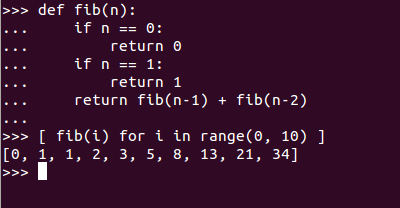
\includegraphics[width=1.0\hsize]{image2012-gum/ipython-pythonshell.png}
      \subfigure{python$B%7%'%k(B}
      \label{pythonshell}
    \end{minipage}
    \begin{minipage}[b]{0.5\textwidth}
      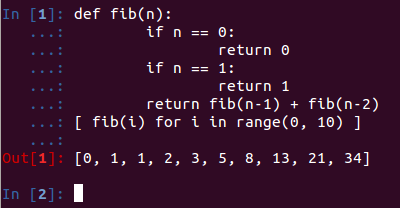
\includegraphics[width=1.0\hsize]{image2012-gum/ipython-terminal.png}
      \subfigure{ipython}
      \label{ipython}
    \end{minipage}
  \end{tabular}
  \caption{python$B%7%'%k$H(Bipython$B$N0c$$(B}
\end{figure*}

\subsection{IPython qtconsole}

ipythopn$B$K(Bqtconsole$B%*%W%7%g%s$r;XDj$7$F<B9T$9$k$3$H$K$h$j!"(B
GUI$B4D6-$G$N(Bipython$B$,5/F0$7$^$9!#(B
$B$^$?$3$N4D6-$G(B \texttt{--pylab inline} $B$r;XDj$7$F5/F0$9$k$3$H$G!"(B
$B%3%s%=!<%kFb$K%0%i%U$rI=<($5$;$k$3$H$,2DG=$H$J$j$^$9!#(B

\begin{commandline}
$ ipython qtconsole --pylab matplotlib
\end{commandline}

$B$3$N4D6-$G$OA0=R$N%0%i%UI=<($K2C$(!"(B
$BJ#?t9T$r$^$H$a$F07$&%3%^%s%I$NMzNr$J$I$,;HMQ$G$-$^$9!#(B
$B%0%i%U$rIA2h$9$k$H<!$N$h$&$KI=<($5$l$^$9!#(B

\begin{figure}[ht]
  \begin{center}
    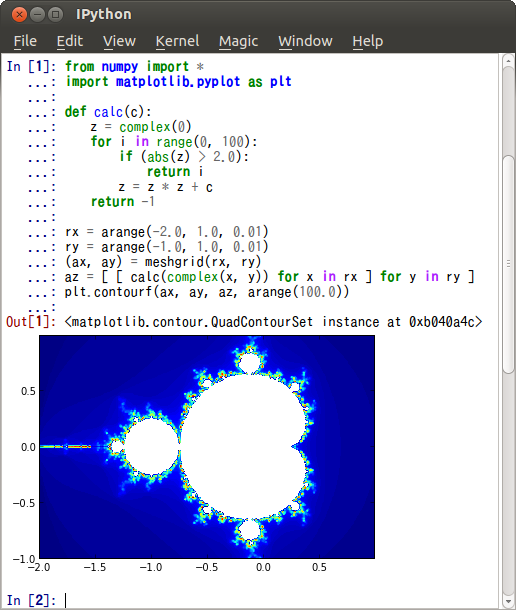
\includegraphics[width=0.6\hsize]{image2012-gum/ipython-mandelbrotset.png}
  \end{center}
  \caption{qtconsole$B$G%^%s%G%k%V%m=89g(B}
  \label{fig:ipython-qtconsole}
\end{figure}

testing$B$G$N(Bipython qtconsole$B$*$h$S(Bmatplotlib$B$O<!$N%3%^%s%I$G%$%s%9%H!<%k=PMh$^$9!#(B

\begin{commandline}
$ sudo aptitude install ipython-qtconsole python-matplotlib
\end{commandline}

$B$^$?(Bsqueeze$B$O(Bbackports$B$r;HMQ$7$F%$%s%9%H!<%k$r9T$$$^$7$?!#(B
$B$^$:(B/etc/apt/sources.list$B$K<!$N9T$rDI2C$7!"(B

\begin{commandline}
deb http://backports.debian.org/debian-backports squeeze-backports main
\end{commandline}

\texttt{aptitude update \&\& aptitude upgrade}$B$r<B9T$7$?8e!"(B
$B<!$N%3%^%s%I$G%$%s%9%H!<%k$7$^$9!#(B

\begin{commandline}
$ sudo aptitude install python-setuptools python2.6-dev ncurses-dev \
  libzmq-dev python-pygments python-matplotlib pyqt4-dev-tools
\end{commandline}

$B%Q%C%1!<%8$N%$%s%9%H!<%k8e!"(B
python$B$N(B\texttt{easy\_install}$B%3%^%s%I$r;HMQ$7$F(Bipython$B$r%$%s%9%H!<%k$7$^$9!#(B

\begin{commandline}
$ sudo easy_install readline pyzmq ipython
\end{commandline}

\subsection{IPython notebook}

ipython notebook$B$O(BWeb$B%Y!<%9$N?t<0=hM}%7%9%F%`$G!"(B
$B<!$N5!G=$rHw$($F$$$^$9!#(B

\begin{itemize}
 \item Python$B%3!<%I$N<B9T$H7k2L$NI=<((B
 \item Markdown$B$K$h$k%^!<%/%"%C%W2DG=$J%N!<%H(B
 \item MathJax$B$K$h$k(B \TeX $B7A<0$G$N?t<0$N5-=R(B
\end{itemize}

\begin{figure}[ht]
  \begin{center}
    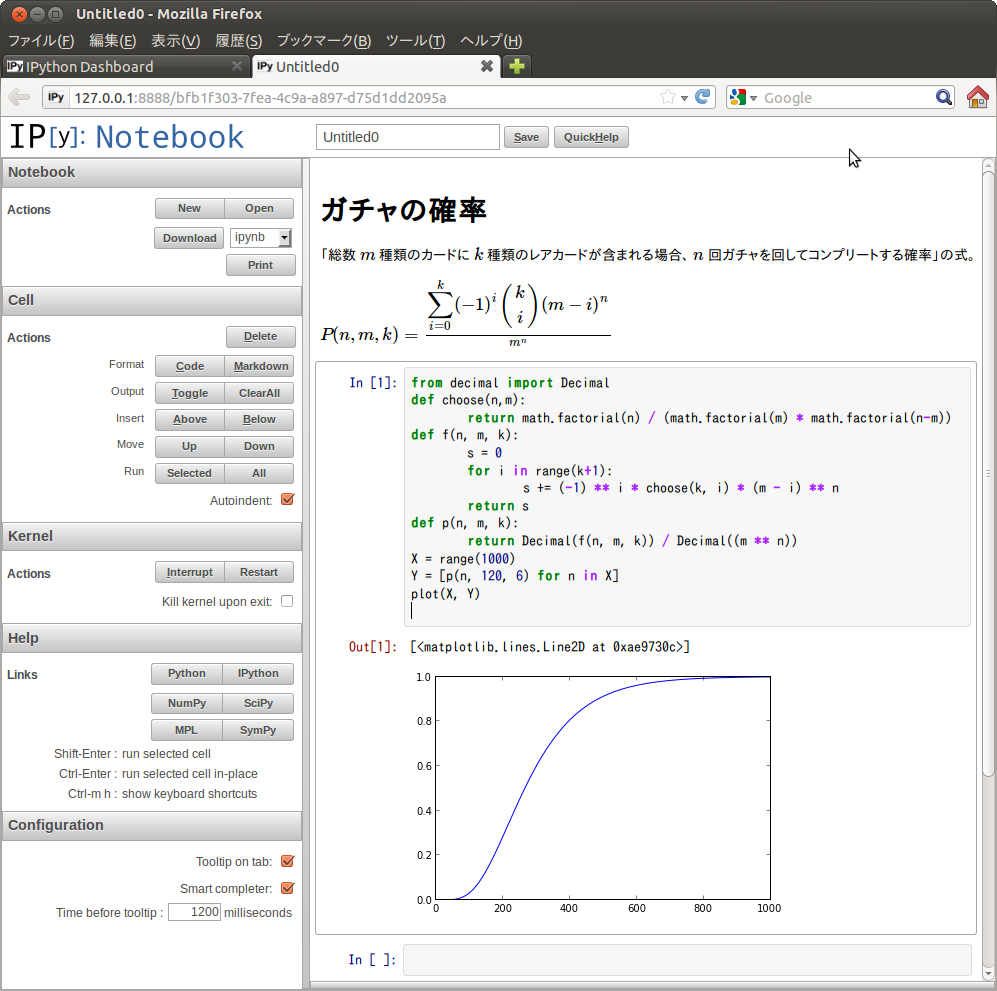
\includegraphics[width=0.80\hsize]{image2012-gum/ipython-gacha.png}
  \end{center}
  \caption{ipython notebook$B$N;HMQNc(B}
  \label{fig:ipython-gacha}
\end{figure}

testing$B$K$O<!$N%3%^%s%I$G%$%s%9%H!<%k2DG=$G$9!#(B

\begin{commandline}
$ sudo aptitude install ipython-notebook python-matplotlib python-tornado
\end{commandline}

squeeze$B$O(Bqtconsole$B$HF1MM$K(Bbackports$B$r;HMQ$7$^$9!#(B
$B$3$3$G$O(Bsqueeze$B$N(Biceweasel$B$,8E$$$?$a$3$A$i$b(Bapt line$B$KDI2C$7$F$$$^$9!#(B

\begin{commandline}
deb http://backports.debian.org/debian-backports squeeze-backports main
deb http://mozilla.debian.net/ squeeze-backports iceweasel-release
\end{commandline}

\texttt{aptitude update \&\& aptitude upgrade}$B$r<B9T$7$?8e!"(B
$B%$%s%9%H!<%k$O<!$N%3%^%s%I$G9T$$$^$7$?!#(B

\begin{commandline}
$ sudo aptitude install python-setuptools python2.6-dev ncurses-dev libzmq-dev python-pygments python-matplotlib
\end{commandline}

$B%Q%C%1!<%8$r%$%s%9%H!<%k$7$?8e!"(B
python$B$N(B\texttt{easy\_install}$B%3%^%s%I$r;HMQ$7$F(Bipython$B$r%$%s%9%H!<%k$7$^$9!#(B

\begin{commandline}
$ sudo easy_install readline pyzmq ipython tornado
\end{commandline}

$B$^$?$3$N$^$^$G$O(BMathJax$B$,(BCDN$B$r;X$7$F$$$k$N$G!"(B
python$B$r4IM}<T8"8B$G<B9T$7%m!<%+%k$K%$%s%9%H!<%k$7$^$9!#(B

\begin{commandline}
from IPython.external.mathjax import install_mathjax
install_mathjax()
\end{commandline}

squeeze$B$N%&%'%V%V%i%&%6$O$I$l$b8E$/!"(B
Web Socket$B$NLdBj$+$i(Bnotebook$B$G$O;H$($^$;$s!#(B
$B$=$3$G:G?7HG$N(Biceweasel$B$rF3F~$7$^$9!#(B
ipython notebook$B$O5/F0;~$K%G%U%)%k%H%V%i%&%6$r5/F0$9$k$?$a!"(B
$BF3F~8e$O(Biceweasel$B$r%G%U%)%k%H%V%i%&%6$K;XDj$7$F$/$@$5$$!#(B

\begin{commandline}
$ sudo aptitude install -t squeeze-backports iceweasel
\end{commandline}

ipython notebook$B$O<!$N%3%^%s%I$G5/F0$7$^$9!#(B

\begin{commandline}
$ ipython notebook --pylab inline
\end{commandline}

$BB>$N%^%7%s$+$i@\B3$r9T$&>l9g!"(B
$B%V%i%&%6$r5/F0$5$;$J$$$?$a%*%W%7%g%s(B``\texttt{--no-browser}''$B$r!"(B
$B%"%/%;%95v2D$rM?$($k$?$a(Bnotebook$B$r5/F0$5$;$k%^%7%s$N(Bip$B%"%I%l%9$r%*%W%7%g%s(B``\texttt{--ip}''$B$G;XDj$7$^$9!#(B

\begin{commandline}
$ ipython notebook --pylab inline --no-browser --ip 192.168.1.40
\end{commandline}

$B=i2s5/F0;~$K$O<!$N$h$&$J2hLL$,I=<($5$l$^$9!#(B

\begin{figure}[ht]
  \begin{center}
    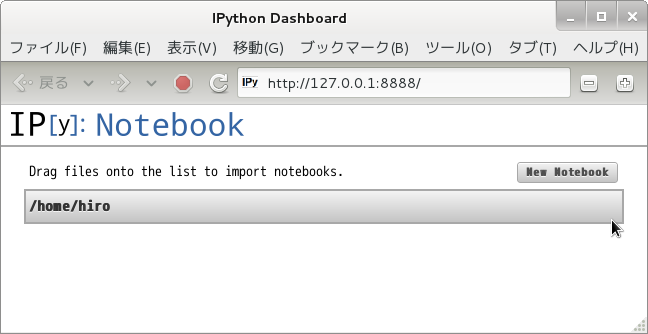
\includegraphics[width=0.67\hsize]{image2012-gum/ipython-notebook.png}
  \end{center}
  \caption{ipython notebook$B$r5/F0$7$?D>8e(B}
  \label{fig:ipython-notebook}
\end{figure}

$B!V(BNew Notebook$B!W%\%?%s$r%/%j%C%/$9$k$3$H$G?75,%N!<%H%V%C%/$,:n@.$5$l!"(B
$B6u$N%N!<%H%V%C%/$,%V%i%&%6$KI=<($5$l$^$9!#(B
Markdown$B$H(BPython$B$N(BCell$B$O(B\texttt{Ctrl-m m}$B$*$h$S(B\texttt{Ctrl-m c}$B$G@Z$jBX$($k$3$H$,$G$-!"(B
$B$=$NB>%3%^%s%I$N>\:Y$O(B\texttt{Ctrl-m h}$B$GI=<($5$l$^$9!#(B

$B:n@.$5$l$?%N!<%H%V%C%/$OI=<($5$l$F$$$k%G%#%l%/%H%j(B($B$3$3$G$O(B/home/hiro/)$B$K(B``$<$ $B%N!<%H%V%C%/$N%?%$%H%k(B$>$.ipynb''$B$H$$$&%U%!%$%kL>$GJ]B8$5$l$^$9!#(B
$B$3$N%U%!%$%k$NCf?H$O(BJSON$B7A<0$H$J$C$F$$$^$9!#(B

\subsection{$B:G8e$K(B}

$B:#2s$O(Bipython qtconsole$B$*$h$S(Bnotebook$B$r(BDebian$B$G;HMQ$9$kJ}K!$r>R2p$7$^$7$?!#(B
Ubuntu 12.04$B$G$O$I$A$i$b%Q%C%1!<%8$H$7$FDs6!$5$l$F$$$k$?$a!"(B
wheezy$B$G$O%$%s%9%H!<%k:n6H$,4JC1$K$J$k$H;W$o$l$^$9!#(B
$B$3$l$r5!2q$K(Bipython$B$r3hMQ$7$F$$$?$@$1$l$P9,$$$G$9!#(B


%------------------------------------------------------------------------------
\dancersection{Debian$B$H(BLibreOffice}{$B$"$o$7$m(B $B$$$/$d(B}
\label{sec:libreoffice}
%------------------------------------------------------------------------------

\subsection{$B<+8J>R2p(B}
\subsection{OOo$B$N$"$i$9$8(B}

\begin{itemize}
\item 1999/8/??$B!D(BSun Microsystems$B$,(BStarOffice$B$N3+H/4k6H$rGc<}(B
\item 2000/10/13$B!D8e$K(BOOo$B$H$J$k%=!<%9%3!<%I8x3+(B
\item 2002/5/1$B!D(BOOo 1.0$B%j%j!<%9(B
\item 2009/4/20$B!D(BOracle$B$K$h$k(BSun$B$NGc<}$rH/I=(B
\item 2010/1/27$B!D(BOracle$B$K$h$kGc<}40N;(B
\item 2010/6/4$B!D(BOOo 3.2.1$B%j%j!<%9(B
\item 2011/1/25$B!D:G=*%P!<%8%g%s$N(B3.3.0$B%j%j!<%9(B
\end{itemize}

\subsection{LibreOffice $B$=$N#1(B}

\begin{itemize}
\item 2010/9/28$B!D(BThe Document Foundation$B$H(BLibreOffice$B$N%j%j!<%9$rH/I=(B
\item OOo$B$N%3%_%e%K%F%#%a%s%P!<$G7k@.(B
\item OOo$B$N>&I8$N0\>y$r(BOracle$B$K5a$a$F$_$?$j(B
\item 2011/1/25$B!D(BLibreOffice 3.3.0$B%j%j!<%9(B
\item 2011/6/3$B!D(BLibreOffice 3.4.0$B%j%j!<%9(B
\item 2012/2/14$B!D(BLibreOffice 3.5.0$B%j%j!<%9(B
\item 2012/2/20$B!D(BTDF$B$,:bCD$K(B
\end{itemize}

\subsection{LibreOffice $B$=$N#2(B}
\subsubsection{$B$+$J$jIaDL$N3+H/BN@)$K$J$C$?(B}

\begin{itemize}
\item $B%=!<%9%3!<%I$O(Bgit$B$G4IM}(B
\item $B7@Ls=q$K%5%$%s$7$J$/$F$b(Bpush$B$5$l$k(B
\item $B%i%$%;%s%9$O(BLGPL$B$H(BMPL
\item $BKh7n%j%j!<%9!"H>G/$K(B1$BEY%a%8%c!<%P!<%8%g%s%"%C%W(B
\item $B:#$O(B8$B7n%j%j!<%9$K8~$1$F(B3.6$B$r3+H/Cf(B
\end{itemize}

\subsection{Apache OpenOffice}

\begin{itemize}
\item 2011/4/15$B!D(BOracle$B$,(BOOo$B$N3+H/Cf;_$rH/I=(B
\item 2011/4/20$B!DC4Ev<R0w$rA40w2r8[(B
\item 2011/6/1$B!D(BApache$B$X$N0\4I$rH/I=(B
\item 2011/6/13$B!D(BApache$B$N(BIncubator$B%W%m%8%'%/%H$K>5G'(B
\item 2011/11/17$B!DL>>N$r!I(BApache Openoffce$B!I$K7hDj(B
\item 2011/11/31$B!D%i%$%;%s%9$r(BAL 2$B$KJQ99$9$k:n6H40N;(B
\item 2012/5/8$B!D(BAOO 3.4.0$B%j%j!<%9(B
\item 2012/5/17$B!D(BAOO 3.4.0 100$BK|%@%&%s%m!<%I(B
\item 2012/5/21$B!D(BLotus Symphony$B$N%3!<%I8x3+(B
\item 2012/5/27$B!D(BAOO 3.4.0 200$BK|%@%&%s%m!<%I(B
\end{itemize}

\subsection{Apache OpenOffice $B$=$N#2(B}
\subsubsection{Lotus Symphony}
\begin{itemize}
\item IBM$B$,(B2008/5/30$B$K%j%j!<%9(B
\item OOo$B$H(BEclipse$B$r%Y!<%9(B
\item Sun$B$+$iFCJL$J%i%$%;%s%9(B
\item $B%o!<%W%m!&I=7W;;!&%W%l%<%s!&(BWeb$B%V%i%&%6(B
\item Windows/Linux$B$GF0:n(B
\item $BL5=~G[I[(B
\item 2012/1/23$B!D:G=*%P!<%8%g%s$N(B3.0.1$B%j%j!<%9(B
\end{itemize}

\subsection{OOo meets Debian}
\subsubsection{$B:G=i$N%"%C%W%m!<%I$O(B2001/10/23}

\begin{itemize}
\item 2002/4/24$B!D(B0.641d.cvs20020424-1$B$r%"%C%W%m!<%I(B
\item 2002/5/1$B!D(BOOo 1.0$B%j%j!<%9(B
\item 2002/5/2$B!D(BOOo 1.0 sid$BF~$j(B
\item 2002/7/11$B!D(BOOo 1.0.1 sid$BF~$j(B
\end{itemize}

\subsubsection{$B8=:_$N%a%s%F%J%s%9BN@)(B}

\begin{itemize}
\item Rene Engelhard$B$5$s$H(BBj\"{o}rn Michaelsen$B$5$s(B(Canonical)$B$NFs?MBN@)(B
\item $B$H$O$$$(!"%Q%C%1!<%8$K4X$7$F$O(BRene$B$5$s$N:n6HNL$,B?$$(B
\item Bj\"{o}rn$B$5$s$O(Bupstream$B$N:n6H$,B?$$(B
\item Bj\"{o}rn$B$5$s$O%S%k%I$N%9%Z%7%c%j%9%H!"(BRene$B$5$s$O%Q%C%1!<%8%s%0$N%9%Z%7%c%j%9%H(B
\end{itemize}

\subsection{LibOffice$B$N%Q%C%1!<%8$NGX7J(B}

\begin{itemize}
\item OOo 3.3.0$B$K4X$9$k:n6H$,9T$o$l$?7A@W$,A4$/$J$$(B
\item $B0JA0$O%Y!<%?HG$G$b:n6H$,9T$o$l$F$$$?(B
\item Rene$B$5$s$O$+$J$jAa$$CJ3,$+$i(BTDF$B$KM6$o$l$F$$$?$3$H$,$o$+$k(B
\item $B3N$+$K(BFounder$B$N0l?M$K$J$C$F$$$k(B\\
\url{http://www.documentfoundation.org/foundation/history/}
\item $B$=$N;~E@$G(BLibO$B$,(BDebian$B$KF~$k$3$H$O3NDjE*$@$C$?(B
\item LibO$B$,(Bsid$B$G;H$($k$h$&$K$J$C$?$N$,(B2012/2/6
\item $B8=:_$G$b(BOpenOffice.org$B$N%Q%C%1!<%8$O$"$k$b$N$N!"(BLibreOffice$B$X$N0\9TMQ%@%_!<%Q%C%1!<%8(B
\end{itemize}

\subsection{LibreOffice$B%Q%C%1!<%8(B}

\subsubsection{libreoffice-3.5.3$B$rNc$K(B}

\begin{itemize}
\item $B%=!<%9$r<hF@8e(Bdf -h$B$9$k$H(B3.2GB
\item rules$B$r(Bwc -l$B$9$k$H(B3146
\item control$B$r(Bwc -l$B$9$k$H(B3380
\item changelog$B$r(Bwc -l$B$9$k$H(B9763
\item buildd$B$G$N%S%k%I;~4V$O(B6$B;~4V(B40$BJ,(B(i386)
\item $BI,MW$J%G%#%9%/%9%Z!<%9$O(B17.04GB
\item $B%Q%C%A$O(Bquilt$B$G4IM}(B
\end{itemize}

\subsubsection{Debian $B%Q%C%1!<%8$NCm0UE@(B}

\begin{itemize}
\item $BF@$F$7$F%*%U%#%7%c%k$N%P%$%J%j$rA0Ds$H$7$?@bL@$r$5$l$k(B
\item $B3HD%5!G=$O0l@Z%$%s%9%H!<%k$5$l$J$$$N$G!"$"$H$+$i%$%s%9%H!<%k$9$k!#$?$$$F$$$O%Q%C%1!<%82=$5$l$F$$$k(B
\item libreoffice-gnome/libreoffice-gtk3/libreoffice-kde$B$N%$%s%9%H!<%k$rK:$l$J$$(B
\end{itemize}

\subsection{LibOffice $B4XO"%Q%C%1!<%8(B}

\begin{enumerate}
\item ooohg \\
Set of 1600 free of charge maps for libreoffice/openoffice.org
\item openclipart-libreoffice \\
clip art for OpenOffice.org/LibreOffice gallery
\item writer2latex \\
OpenOffice.org Writer/Calc to LaTeX/XHTML converter
\end{enumerate}

\subsection{$BK]Lu$N$3$H(B}
\subsubsection{$B3'$5$s$K$*4j$$(B}
\begin{itemize}
\item \url{discuss@ja.libreoffice.org}$B$r9XFI$7$F$M(B
\item $BK]Lu$N;XE&!J8mLu$d$o$+$j$K$/$$$b$N$J$I!K(B
\item $B@lLgE*$JCN<1$N65<((B
\item $B1Q8l!"F|K\8l!"%o!<%W%m!"I=7W;;!JFC$K4X?t!K!"%I%m!<!"(BWindows$B!"(BMac$B!"(BLinux$B!"?t<0!"%G!<%?%Y!<%9!"(BPDF$B!"0u:~(B etc...
\item $B4V@\E*$K(BDebian$B$X$N9W8%$K$b$J$j$^$9$h!*(B
\end{itemize}

\subsection{AOO $B$H(B Debian}
\subsubsection{6$B7n>e=\8=:_!"%Q%C%1!<%8$J$7(B}
\begin{itemize}
\item $B2x$7$$%j%]%8%H%j$O$"$k(B\\
\url{http://apacheoo-deb.sourceforge.net/}
\item $B%*%U%#%7%c%k%S%k%I$N(BDeb$B%Q%C%1!<%8$r(Bapt$B$G<h$l$k$h$&$K$7$F$$$k$@$1(B
\item $B$A$J$_$K(Blaunchpad$B$K%W%m%8%'%/%H$O$"$k$1$I%Q%C%1!<%8$O$J$$(B\\
\url{https://launchpad.net/~apacheopenoffice}
\end{itemize}

\subsubsection{$B%*%U%#%7%c%k%S%k%I$N(BDeb$B%Q%C%1!<%8(B}
\begin{itemize}
\item EPM$B$G@8@.(B
\begin{itemize}
\item ESP Package Manager
\item $B$3$l$O(BLibreOffice$B$b0l=o(B
\item $B86:n<T$O(BCUPS$B$N:n<T(B
\item RPM$B$H$+(BDeb$B%Q%C%1!<%8$r@8@.$9$k$b$N(B
\item $B$9$J$o$A!"(Bdebian$B%U%)%k%@$,$"$k$o$1$8$c$J$$(B
\item $B$I$&$d$C$F$b%*%U%#%7%c%k$K$J$i$J$$(B
\end{itemize}
\end{itemize}
\subsubsection{3$B7n$K(Bdebian-users$B$H(Bdebian-openoffice$B$G(BAOO$B$K4X$9$kEj9F$"$j(B}
\begin{itemize}
\item \url{http://lists.debian.org/debian-user/2012/03/msg00824.html}
\item \url{http://lists.debian.org/debian-openoffice/2012/03/msg00103.html}
\end{itemize}
$B$$$:$l$b(BRene$B$5$s$,7c$7$/5qH](B

\subsection{$B$5$i$J$k>pJs(B}
\subsubsection{$B<g$KNr;K$rCN$j$?$$?M8~$1(B}
\begin{enumerate}
\item 2011$BG/$N(BOpenOffice.org/LibreOffice
\\
\url{http://gihyo.jp/lifestyle/column/newyear/2011/openoffice-prospect}
\item LibreOffice/Apache OpenOffice $B!A(B2011$BG/$NAm3g$H?7$?$JA*Br!A(B
\\
\url{http://gihyo.jp/lifestyle/column/newyear/2012/libreoffice-prospect}
\end{enumerate}

%------------------------------------------------------------------------------
\dancersection{debug.debian.net}{$B4d>>(B $B?.MN(B}
\label{sec:debug.debian.net}
%------------------------------------------------------------------------------

\subsection{$B$O$8$a$K(B}
$B8=:_!"(BDebian Project $B$GG[I[$5$l$F$$$k%Q%C%1!<%8$G$O!"(B
$B%G%P%C%0>pJs$,:o=|$5$l$?>uBV$GG[I[$5$l$F$$$^$9!#(B
$B$3$NM}M3$H$7$F!"%G%P%C%0>pJs$O$[$H$s$I$N%f!<%6$K$OI,MW$J$$$b$N$G$"$k$H$$$&E@$H!"(B
$B%G%P%C%0>pJs$rJ];}$7$F$$$k<B9T%U%!%$%k$O%5%$%:$,Hs>o$KBg$-$$$?$a!"%G%#%9%/$r05Gw(B
$B$9$k$H$$$&E@$,$"$j$^$9!#(B
$B$7$+$7!"%G%P%C%0>pJs$,$"$k$H%G%P%C%0$r9T$&$H$-$K$H$F$bM-MQ$J>pJs$H$J$j$$$m$$$m$HJXMx$G$9!#(B
$B:#2s!"(BDebian $B$GA4$F$N(BDebian$B%Q%C%1!<%8$K$*$$$F%G%P%C%0>pJs$rDs6!$9$kJ}K!$r9M$($F<BAu$7$F$_$^(B
$B$7$?!#$=$N2]Dx$H:#8e$K$D$$$F@bL@$7$^$9!"(B

\subsection{Debug$B>pJs$H(BDebian$B%Q%C%1!<%8(B}
Debian $B$O%P%$%J%j%Y!<%9%G%#%9%H%j%S%e!<%7%g%s$N0l$D$G$9!#(B
$B4pK\E*$KG[I[$5$l$F$$$k%Q%C%1!<%8$G$O%G%P%C%0>pJs$,:o=|$5$l$?>uBV$GG[I[$5$l$F$$$^$9!#(B
$B$3$N%G%P%C%0>pJs$O!"FbIt%7%s%\%k$d7?$N>pJs!"%=!<%9%3!<%I$N9THV9f$J$I$r;X$7$^$9!#(B

$B<B9T%U%!%$%k$N%G%P%C%0>pJs$,$"$k>l9g!"0J2<$N$h$&$J$h$$E@$,$"$j$^$9!#(B
\begin{itemize}
\item $B%G%P%C%,!J(BGDB$B!K$r;H$C$?%G%P%C%0$G$h$j>\:Y$J%G%P%C%0>pJs$rF@$k$3$H(B
$B$,$G$-$k(B
\item $B%G%P%C%0>pJs$r4^$a$?%P%$%J%j$r:FEY%S%k%I$9$kI,MW$,$J$$(B
\item $B%P%$%J%j%Y!<%9%G%#%9%H%j%S%e!<%7%g%s$N>l9g!"<B:]$N%P%$%J%j$H%G%P%C%0>pJs$,>o$K(B
$BBP$K$J$k$N$G!"%P%0$N:F8=@-$,9b$/$J$k(B
\end{itemize}
%$B$3$l$i$OAH$_9~$_MQES$K$b$h$/MxMQ$5$l$F$$$k(BDebian$B$G$OFC$KM-8z$KF/$-$^$9!#(B
%$B$^$?!"%G%P%C%0>pJs$r4^$a$k$?$a$N%Q%C%1!<%8:n@.J}K!!J(BDEB_BUILD_OPTIONS=nostrip $B$r$r4D6-(B
%$BJQ?t$K%(%/%9%]!<%H$9$k!K$rD4$Y$kI,MW$b$"$j$^$;$s!#(B

$B5U$K0-$$E@$H$7$F0J2<$N$h$&$J$b$N$,$"$j$^$9!#(B

\begin{itemize}
\item $B<B9T%U%!%$%k$K%G%P%C%0>pJs$,4^$^$l$k$N$G<B9T%U%!%$%k$N%5%$%:$,Bg$-$/$J$k(B
\item $B%G%P%C%0$7$J$$?M$K$H$C$F$OITMW$J$b$N$,4^$^$l$k$3$H$K$J$k(B
\end{itemize}

$B$3$l$i$r$^$H$a$k$H!"$9$Y$F$N<B9T%U%!%$%k$N%G%P%C%0>pJs$,Ds6!$5$l$F$*$j(B
$B%f!<%6$K$H$C$FI,MW$N$J$$>pJs$,%$%s%9%H!<%k$5$l$J$$;EAH$_$,$"$l$P(B
$B%G%P%C%0>pJs$O$H$F$bM-1W$J$b$N$K$J$k$O$:$G$9!#(B
Debian $B$G$O$$$/$D$+$N%=!<%9%Q%C%1!<%8$+$i%G%P%C%0>pJs$r4^$s$@%Q%C%1!<%8$,Ds6!$5$l$F$$$^$9!#(B
$B$3$N%Q%C%1!<%8$K$O(B\texttt{-dbg} $B$H$$$&%5%U%#%C%/%9$,IU$$$F$^$9!#(B
$BFC$K%G%P%C%0>pJsMQ$N%Q%C%1!<%8$K4X$9$k%]%j%7!<$O7h$^$C$F$*$i$:!"Ds6!$K4X$7$F$O%Q%C%1!<%8%a%s%F%J(B
$B<!Bh$H$$$&>uBV$K$J$C$F$$$^$9!#:#$^$GDs6!$5$l$J$+$C$?M}M3$H$7$F$O%G%#%9%/MFNL$NLdBj$d2s@~$N(B
$BLdBjEy$,$"$C$?$h$&$G$9$,!"8D?ME*$K:#$OFC$KLdBj$O$J$$$H;W$C$F$$$^$9!#(B

$B$A$J$_$K!"(BFedora$B$G$O(B \texttt{-debuginfo} $B$H$$$&%5%U%#%C%/%9$r;}$C$?%Q%C%1!<%8$,Ds6!$5$l$F$*$j!"(B
Gentoo$B$G$O%G%U%)%k%H$G$3$l$i$N>pJs$r@8@.$74IM}$7$F$$$^$9!#$3$N$h$&$K%G%P%C%0>pJs$NDs6!$H$$$&E@$K(B
$B4X$7$FB>$N%G%#%9%H%j%S%e!<%7%g%s$KCY$l$r<h$C$F$$$^$9!#(B

\subsection{Debian$B$G$N%G%P%C%0>pJs%Q%C%1!<%8$K$D$$$F(B}
$B$^$:!"<BAu$7$?FbMF$K$D$$$F@bL@$9$kA0$K:#$N%G%P%C%0>pJs%Q%C%1!<%8$NDs6!J}K!$K$D$$$F@bL@$7$^$9!#(B
Debian$B$G$O%G%P%C%0>pJs%Q%C%1!<%8$O(B \texttt{-dbg} $B$H$$$&%5%U%#%C%/%9$,$D$$$?%Q%C%1!<%8L>$r;}$A$^$9!#(B
$BNc$($P(B foo $B$H$$$&%"!<%-%F%/%A%c0MB8$N%Q%C%1!<%8$,$"$C$?>l9g!"(B\texttt{foo} $B$N%G%P%C%0>pJs$r;}$C$?%Q%C%1!<%8L>$O(B
\texttt{foo-dbg} $B$K$J$j$^$9!#(B
$B$=$7$F!"(BDebian $B$N(B \texttt{-dbg} $B%Q%C%1!<%8$GDs6!$5$l$F$$$k%P%$%J%j$OF0:n$9$k%P%$%J%j%G!<%?$G$O$J$/!"(B
$B%G%P%C%0>pJs$N$_$r;}$C$?%G!<%?$K$J$C$F$$$^$9!#(B $B$3$N%U%!%$%k$O(B \texttt{objdump --only-keep-debug}
$B$r<B9T$9$k$3$H$K$h$C$F@8@.$9$k$3$H$,$G$-$^$9!#$b$A$m$sBP>]$N<B9T%U%!%$%k$O%3%s%Q%$%k;~$K%G%P%C%0>pJs(B
$B$,IU2C$5$l$F$$$kI,MW$,$"$j$^$9!#(B
$B$=$N8e!"%G%P%C%0>pJs%U%!%$%k$X$N%j%s%/$r(B \texttt{strip} $B:Q$N<B9T2DG=7A<0$KIU2C$9$k$?$a$K(B
\texttt{objcopy --add-gnu-debuglink} $B$r<B9T$7$^$9!#(B
$B$3$l$K$h$C$F!"<B9T%U%!%$%k$H%G%P%C%0>pJs%U%!%$%k$,BP$K$J$j$^$9!#(B
GDB $B$r;H$C$F%G%P%C%0$9$k:]$K$O<B9T%U%!%$%k$H%G%P%C%0>pJs%U%!%$%k$O%j%s%/(B
$B$7$F$$$k$N$G!"%G%P%C%0>pJs%U%!%$%k$,%$%s%9%H!<%k$5$l$F$$$k$H$-$O<+F0E*$K8F$P$l!"%G%P%C%0(B
$B%7%s%\%k$J$I$rFI$_9~$s$G$/$l$^$9!#(B

\subsection{$B<BAu$K$D$$$F(B}

$B@h$K@bL@$7$?$h$&$K$K!"$9$Y$F$N<B9T%U%!%$%k$N%G%P%C%0>pJs$,Ds6!$5$l$F$*$j(B
$B%f!<%6$K$H$C$FI,MW$N$J$$>pJs$,%$%s%9%H!<%k$5$l$J$$;EAH$_$,$"$l$P$h$$$N$G!"(B
$B$3$l$i$KBP1~$G$-$kJ}K!$r9M$($^$7$?!#0J2<$G@bL@$7$^$9!#(B

\subsubsection{$B$9$Y$F$N<B9T%U%!%$%k$N%G%P%C%0>pJs$rDs6!$9$k(B}
$B$9$Y$F$N<B9T%U%!%$%k$N%G%P%C%0>pJs$rDs6!$9$k$K$O!"A4$F$N%Q%C%1!<%8$G(B
\texttt{strip} $B$5$l$?<B9T%U%!%$%k$H%G%P%C%0>pJs%U%!%$%k$r;}$C$?%Q%C%1!<%8$r9=C[$9$l$P(B
$B$h$$$o$1$G$9!#(B


Debian $B$N>l9g!"%Q%C%1!<%8$O%G%P%C%0>pJs$,M-8z$J>uBV!J(B\texttt{gcc} $B$@$H(B\texttt{-g} $B%*%W%7%g%sEy!K(B
$B$G%S%k%I$5$l$^$9!#$=$7$F%Q%C%1!<%8$K$5$l$k;~$K(B \texttt{strip} $B!J(Bbinutils$B$K4^$^$l$k!K(B
$B$,(B \texttt{dh\_strip} $B$+$i8F$P$l!"<B9T%U%!%$%k$d%i%$%V%i%j$J$i%G%P%C%0>pJs$,:o=|$5$l!"(B
$B%Q%C%1!<%8MQ$N%G%#%l%/%H%j$K%3%T!<$5$l!"(B\texttt{dh\_builddeb} $B%3%^%s%I$G%Q%C%1!<%82=$5$l$^$9!#(B

$B$=$7$F!"G[I[$5$l$k(B -dbg $B%Q%C%1!<%8$O(B \texttt{dh\_strip}$B$r<B9T$9$k$H$-$K%G%P%C%0>pJs$rDs6!$9$k(B
$B%Q%C%1!<%8$H$7$F!"(B\texttt{dh\_strip} $B$N%*%W%7%g%s$H$7$F;XDj$5$l$k$+!"(Bdebian/control $B%U%!%$%k$KNs5s$5$l$F$$$k(B
$B%Q%C%1!<%8L>$N%5%U%#%C%/$K(B \texttt{-dbg} $B$,IU$$$F$$$k>l9g!"BP>]%U%!%$%k$H$7$F=hM}$5$l$^$9!#(B

$B$3$3LdBj$J$N$,!"(B
\begin{enumerate}
\item $B<+F0@8@.$7$?$$(B $B%G%P%C%0>pJs%Q%C%1!<%8>pJs$r$I$N$h$&$K@8@.$9$k$+(B
\item \texttt{dh\_strip} $B$G%G%P%C%0>pJs%Q%C%1!<%8;XDj$5$l$F$$$k>l9g!"<+F0@8@.$7$?$$(B -dbg $B%Q%C%1!<%8MQ$N%U%!%$%k$r(B
$B$I$N$h$&$K@8@.$9$k$+(B
\item $B<+F0@8@.$7$?$$%G%P%C%0>pJs%Q%C%1!<%8$=$N$b$N$r$I$N$h$&$K@8@.$9$k$+(B
\end{enumerate}
$B$H$$$&E@$G$9!#(B

$BLdBjE@#1$K$D$$$F$NBP=hJ}K!$G$9$,!"(B\texttt{dh\_strip} $B$N=hM}$N@hF,$G(B debian/control $B%U%!%$%k$K(B
$B%G%P%C%0>pJs%Q%C%1!<%8%U%!%$%k$K4X$9$k>pJs$rDI5-$9$k=hM}$rDI2C$7$^$7$?!#(B
$B%G%P%C%0>pJs%Q%C%1!<%8$O$=$N%Q%C%1!<%8$,%"!<%-%F%/%A%c0MB8!J(BArchitechture: all $B$G$O$J$$!K(B
$B;v$H%Q%C%1!<%8L>$5$($o$+$l$P!"%Q%C%1!<%8>pJs$O<+F0@8@.$G$-$^$9!#(B
$BNc$($P!"(B\texttt{hoge} $B$H$$$&%Q%C%1!<%8$,$"$C$F%G%P%C%0>pJs%Q%C%1!<%8$,Ds6!$5$l$F$$$J$$>l9g!"(B
$B0J2<$N$h$&$JFbMF$rDI5-$7$^$9!#(B

\begin{commandline}
Package: hoge-dbg
Architecture: any
Section: debug
Priority: extra
Depends: hoge (= \${binary:Version}), \${misc:Depends}
Description: debugging symbols for hoge
 This package contains the debugging symbols for hoge
\end{commandline}

$B<!$KLdBjE@#2$NBP=hJ}K!$G$9$,!"%"!<%-%F%/%A%c0MB8$N(BDebian$B%Q%C%1!<%8$O(B \texttt{dh\_strip} $B$,8F$P$l$k$?$a!"$3$3$G(B
$B=hM}$r%U%C%/$7$F$7$^$($P!"%G%P%C%0>pJs$rDs6!$9$k%Q%C%1!<%8$HMQ$N%G!<%?$H(B \texttt{strip} $B$5$l$?(B
$B%P%$%J%j%G!<%?$rJ,$1$k$3$H$,$G$-$^$9!#:#2s$O(B \texttt{dh\_strip} $B$NCf?H$r2~B$$7!"A4$F$N%"!<%-%F%/%A%c0MB8$N(B
$B%Q%C%1!<%8MQ$N%G!<%?$r:n@.$9$k$3$H$K$7$^$7$?!#(B\texttt{dh\_strip}$B$G%Q%C%1!<%8$,;XDj$5$l$F$$$F$b(B
$B$=$l$rL5;k$9$k$h$&$K=hM}$rJQ99$9$k$@$1$G$9!#(B

$BLdBjE@#3$NBP=hJ}K!$G$9$,!"%G%P%C%0>pJs%Q%C%1!<%8$O(B \texttt{dh\_strip} $BFb$G(B \texttt{dh\_builddeb} $B$r8F$S=P$9$3$H$G(B
$BBP1~$7$^$7$?!#%Q%C%1!<%8L>$H%Q%C%1!<%8:n@.$KI,MW$J%G!<%?$OB7$C$F$$$k$N$G!"(B
\texttt{dh\_builddeb -p$B%G%P%C%0>pJs%Q%C%1!<%8L>(B} $B$r<B9T$9$k$3$H$G!"%Q%C%1!<%8$,:n@.$5$l$^$9!#(B

$B$3$l$i$,9T$($kA0Ds>r7o$H$7$F!"(Bdebhelper $B$K0MB8$7$F$$$k%Q%C%1!<%8$,BP>]$K$J$j$^$9!#(B
$B8=:_$[$H$s$I$N%Q%C%1!<%8$,(B debhelper $B$+(B CDBS $B$K0MB8$7$F$*$j!"(BCDBS $B$O(B debhelper $B$H(B
$BF1;~$K;H$&;v$,B?$$$?$a!J<B:]!"(BCDBS$B$K0MB8$7$F$$$k%Q%C%1!<%8$OA4$F(Bdebhelper $B$K0MB8$7$F$$$^$9!#(Bdbs$B$bF1MM$G$9!#!K(B
$BLdBj$G$O$"$j$^$;$s!#(B
\footnote{\url{http://people.debian.org/~cjwatson/dhstats.png}}

\subsection{$B%Q%C%1!<%8%5%$%:$X$NBP1~(B}

$B<!$K%Q%C%1!<%8%5%$%:$NLdBj$G$9!#(B
$B%G%P%C%0>pJs$OHs>o$KBg$-$/!"(B\texttt{strip} $B$5$l$?%P%$%J%j$N?tG\0J>e$N%5%$%:$K$J$k$3$H$O(B
$B$a$:$i$7$/$"$j$^$;$s!#Nc$($P(B libjpeg8 $B$GDs6!$5$l$k(B libjpeg.so.8.4.0 $B$N%U%!%$%k(B
$B%5%$%:$OI=(B\ref{tab:debuginfo-jpegsize}$B$H$J$j$^$7$?!#(B

\begin{table}[ht]
 \caption{libjpeg.so.8.4.0 $B3F>uBV$N%U%!%$%k%5%$%:(B}
 \label{tab:debuginfo-jpegsize}
\begin{center}
  \begin{tabular}{|c|c|}
 \hline
 $B>uBV(B & $B%5%$%:(B \\
 \hline
 strip $BA0(B & $BLs(B1.3MB \\
 strip $B8e(B & 236KB \\
 $B%G%P%C%0>pJs%U%!%$%k(B & 1.1MB \\
 \hline
 \end{tabular}
\end{center}
\end{table}

$B$3$N$h$&$K%5%$%:$,Bg$-$/0[$J$k$N$G!"%Q%C%1!<%8$rJ,$1$F$b%f!<%6$,MxMQ$7$F$$$k%Q%C%1!<%8%j%]%8%H%j(B
$B$HF1$8>l=j!&J}K!$GDs6!$7$F$7$^$&$H!"%_%i!<$K;~4V$,$+$+$k$h$&$K$J$j$^$9$7%f!<%6$KITMW$J%G!<%?$,3JG<$5$l$?%j(B
$B%]%8%H%j>pJs$r;}$?$;$k$h$&$K$J$j$^$9!#(B

$B:#2s!"$3$NLdBj$r2sHr$9$k$?$a$K%j%]%8%H%j$rJ,$1$k$3$H$r9M$($^$7$?!#(B
$BNc$($P!"(Bunstable $B$G(B \texttt{strip} $B$5$l$F$$$k%Q%C%1!<%8!JDL>o$N%Q%C%1!<%8!K$O(B unstable $B$H$@$1;XDj$7!"(B
$B%G%P%C%0>pJs$rDs6!$9$k%Q%C%1!<%8$O(B unstable/debug $B$9$k$H$$$&J}K!$G$9!#(B
$BNc$r?^(B\ref{fig:debuginfo-apt-line}$B$K<($7$^$9!#(B

\begin{figure}[ht]
\begin{center}
\begin{commandline}
deb http://cdn.debian.or.jp/debian/ unstable main non-free
deb http://cdn.debian.or.jp/debian/ unstable/debug main
\end{commandline}
\end{center}
 \caption{$B%G%P%C%0>pJs%Q%C%1!<%8$rMxMQ$9$k>l9g$N(B apt-line $B@_DjNc(B}
 \label{fig:debuginfo-apt-line}
\end{figure}


$B%G%P%C%0>pJs$,I,MW$J%f!<%6$O(B unstable/debug $B$r(B apt-line $B$KDI2C$9$k$3$H$K$h$C$F%G%P%C%0>pJs(B
$BMQ$N%Q%C%1!<%8$,MxMQ$G$-$k$h$&$K$J$j$^$9!#(B
$B$^$?%Q%C%1!<%8$,3JG<$5$l$k%G%#%l%/%H%j$N%Q%9$rJQ99$9$k$3$H$K$h$C$F!"%G%P%C%0>pJs$N$_$r(B
$BDs6!$9$k%_%i!<$r9=C[$9$k$3$H$,$G$-!"(Bdebug $B>pJs$r%_%i!<$7$J$$%_%i!<%5!<%P$NIi2Y$b:#$^$G$HJQ$o(B
$B$i$J$$$H$$$&;v$K$J$j$^$9!#(B

\subsubsection{$B<BAu8e$K$D$$$F(B}

$B$3$l$i$r<BAu$7$?%7%9%F%`$r(B reprepro + sbuild + rebuildd $B$G9=C[$7$^$7$?!#(B
$B8=:_(Bstable/amd64$B$N$_$r%?!<%2%C%H%F%9%H$H$7$FF0:n$5$;$F$$$^$9!#(B
$B$^$@A4$F%S%k%I$G$-$F$$$^$;$s!#$5$/$i$N(BVPS$B$G#1=54V$[$I%S%k%I$7$F$$$^$9$,!"(B
$B$^$@(Bgnome-power-manager$B$r%S%k%I$7$F$$$k$H$3$m$G!"?JD=N($O(B40\%$B$H$$$C$?$H$3$m$G$7$g$&$+!#(B

\subsection{$B9M$($i$l$kLdBj(B}

\subsubsection{$B%;%-%e%j%F%#$NLdBj(B}
$B8=:_!"%=!<%9%Q%C%1!<%8$+$i:n@.$5$l$?%P%$%J%j%P%C%1!<%8$N0lMw$O(B .changes$B%U%!%$%k$K(B
$B%U%!%$%k$N%O%C%7%e$H6&$K5-=R$5$l!"$I$N%=!<%9%Q%C%1!<%8!J(Borig.tar.gz, dsc.diff.gz$B!K(B
$B$+$i:n@.$5$l$?$N$+J,$+$k$h$&$K$J$C$F$$$^$9!#(B
$B8=;~E@$G$N<BAu$O%P%$%J%j%Q%C%1!<%8:n@.$N2]Dx$G<+F0@8@.$5$l$k$?$a$N$3$l$i$N>pJs(B
$B$H%j%s%/$7$^$;$s!#(BBuildd$B>e$G%G%P%C%0>pJs%U%!%$%k%Q%C%1!<%8$,@8@.$5$l$k$N$G8D?ME*$K(B
$BLdBj$J$$$H;W$C$F$$$^$9$,!"$3$l$i$rI3IU$1$k%7%9%F%`$,$"$k$[$&$,$h$j0BA4$H8@$($k$G$7$g$&!#(B

\subsubsection{$B%P%$%J%j$NIT0lCW(B}
$B4{B8$N%7%9%F%`$@$H!"(B\texttt{strip} $B$5$l$?%P%$%J%j$H(B $B%G%P%C%0>pJs$,0lCW$7$J$$$N$G(B
$B%*%U%#%7%c%k$N%P%$%J%j$H:.$<$F;H$($J$$$3$H$,9M$($i$l$^$9!#;d$,Ds6!$7$F$$$k(B
$B$5$l$F$$$k%G%P%C%0>pJs%Q%C%1!<%8$r;H$&>l9g!"(B
$B;d$,Ds6!$7$F$kDL>o$N%Q%C%1!<%8$bMxMQ$7$J$$$H0UL#$,$J$$$G$7$g$&!#(B
$B:#$O$3$l$r%P!<%8%g%s$K$h$k0MB84X78$G2sHr$7$F$$$^$9!#(B
$B:G=*E*$K$O(B buildd $B$KF~$l$F$b$i$&$3$H$G%G%P%C%0>pJs%Q%C%1!<%8$r<+F0@8@.$9$k$3$H$r(B
$B9M$($F$$$^$9!#(B

\subsection{$B$=$b$=$b(B debug.debian.net$B$,$"$k$s$8$c$M!)$H$$$&OC(B}
$B$5$F!";d$N$h$&$JK^?M$,9M$($k$h$&$J$3$H$O@h?MC#$O$9$G$K9M$($F$$$k$o$1$G$7$F!"(B
$B!J4{$K9T$J$C$F$$$k$3$H$rCN$C$?$N$OBgE}0lJY6/2q%9%1%8%e!<%k$,=P$F$+$i$J$N$G$9$,!#!K(B
$B4{$K(B \url{http://debug.debian.net}$B$H$$$&%5!<%S%9$,$"$j<BAu$5$l!"$=$7$F=*N;$7$F$$$^$7$?!#(B
$B<BAu$H9M$($b$[$H$s$IF1$8$G$9!#Bg$-$/0c$&$H$3$m$O%G%P%C%0>pJs%Q%C%1!<%8$N(B
$B%5%U%#%C%/%9$,(B\texttt{-dbg}$B$G$O$J$/!"(B\texttt{-dbgsym}$B$G$"$kE@$H!"(B
$B%G%P%C%0>pJs$r:n@.$9$kItJ,$,(B \texttt{dh\_builddeb} $B$G$O$J$/!"(B\texttt{dpkg-deb} $B$r;H$C$F$$$k(B
$BE@!"$=$7$F(B\texttt{dh\_strip}$B$rD>@\JQ99$9$k$N$G$O$J$/!"%7%s%\%j%C%/%j%s%/$G(B
$B5!G=$r%*!<%P!<%i%$%I$5$;$F$$$kE@$G$9!#$3$A$i$NJ}$,(Bdebhelper$B$K<j$r2C$($J$/$F:Q$`$N$G(B
$B$3$A$i$K>h$j49$($F!"$$$/$D$+$N=$@5$r9T$$$^$7$?!#(B
$B85!9$3$N%5!<%S%9$O(B myon \footnote{Christoph Berg$B;a!#(BDAM $B$N0l?M!#(B} $B$,$d$C$F$$$?$N$G$9$,!"(B
$BH`$KO"Mm$r<h$j!":F2TF/$5$;$k$3$H$K$7$^$7$?!#$3$NH/I=$,9T$o$l$F$$$k:"$K$O2TF/$7$F$$$k$H;W$$$^$9!#(B

\subsection{$B:#8e$N2]Bj(B}

$B$3$N$^$^%9%?%s%I%"%m%s$G%G%P%C%0>pJs%Q%C%1!<%8$rDs6!$7$F$bL5BL$J%P%$%J%j$r@8@.$9$k$@$1$J$N$G!"(B
buildd $B$K$3$N%7%9%F%`$rF~$l$F$b$i$$!"(Bdak $B$G(B $B%G%#%9%H%j%S%e!<%7%g%s(B/debug $B$H$7$F(B
$B=hM}$7$F$b$i$&$3$H$,:#8e$NBg$-$J2]Bj$K$J$C$F$$$^$9!#$3$N$3$H$K$D$$$FMh7n3+:E$5$l$k(B Debconf 12
$B$G(BBOF $B$^$?$O(BFTP$B%A!<%`!"(Bwanna-buildd$B%A!<%`$HOC$,$G$-$l$P$H;W$C$F$$$^$9!#(B

\subsection{$B:G8e$K(B}
$B%"!<%-%F%/%A%c$K0MB8$7$F$$$k(B Debian $B%Q%C%1!<%8$G%G%P%C%0>pJs$r(B
$B%Q%C%1!<%8$H$7$FDs6!$9$kJ}K!$K$D$$$F@bL@$7$^$7$?!#J8Cf$G$O%f!<%6$K$O(B
$B$"$^$jI,MW$N$J$$5!9=$N$h$&$K<h$j07$$$^$7$?$,!"%P%0%l%]!<%H$r$9$k:]!"(B
$B%G%P%C%0>pJs$,$"$k$H$h$jFbMF$NG;$$%P%0%l%]!<%H$rDs=P$G$-$k$h$&$K$J$j!"(B
$B3+H/<T$r<j=u$1$G$-$k$h$&$K$J$j$^$9!#$3$N5!9=$,@5<0:NMQ$5$l$?;~$K!"(B
$B<+J,$,;H$C$F$$$k%Q%C%1!<%8$N%G%P%C%0>pJs%Q%C%1!<%8$@$1$G$b%$%s%9%H!<%k(B
$B$7$F$/$l$l$P9,$$$G$9!#(B

%------------------------------------------------------------------------------
\dancersection{Rabbit: $B;~4VFb$K=*$o$l$k%W%l%<%s%D!<%k(B}{$B?\F#8yJ?(B}
\label{sec:Rabbit}
%------------------------------------------------------------------------------

% add upper space for logo
\vspace{2em}

Debian GNU/Linux$B>e$GF0:n$9$k%W%l%<%s%F!<%7%g%s%D!<%k(BRabbit$B$r>R2p$7$^$9!#(B
$B$^$:!"(BRabbit$B$NBeI=E*$J5!G=$G$"$k;~4VFb$K=*$o$l$k$?$a$N5!G=$r>R2p$7!"$=(B
$B$N8e!"(BDebian GNU/Linux$B>e$G(BRabbit$B$r%$%s%9%H!<%k$9$kJ}K!$H%9%i%$%I$r:n$k(B
$BJ}K!$r4JC1$K>R2p$7$^$9!#(B

\subsection{Rabbit$B$H$O(B}

Rabbit$B$O(BRuby$B$H(BGTK+$B$G<BAu$5$l$?%W%l%<%s%F!<%7%g%s%D!<%k$G$9!#(BDebian
GNU/Linux$B$r4^$`B?$/$N%W%i%C%H%U%)!<%`>e$GF0:n$7$^$9!#(B

Debian GNU/Linux$B>e$GF0:n$9$k%W%l%<%s%F!<%7%g%s%D!<%k$O$?$/$5$s$"$j$^$9!#(B

\begin{itemize}
\item GUI$B$G%9%i%$%I$r:n@.$9$k%G%9%/%H%C%W%"%W%j%1!<%7%g%s(B
  $B!J(BLibreOffice$B$N(BImpress$B$J$I!K(B
\item $B%F%-%9%H$G:n@.$7$?%9%i%$%I$rI=<($9$k%G%9%/%H%C%W%"%W%j%1!<%7%g%s(B
  $B!J(BMagicPoint$B$d(BRabbit$B$J$I!K(B
\item \LaTeX{}$B$N(BBeamer$B%/%i%9(B + PDF$B%S%e!<%"!<!J(BEvince$B$d(Bpdfcube$B$J$I!K(B
\item JavaScript + Web$B%V%i%&%6!J(BImpress.js$B$d(Bshowoff$B$J$I!K(B
\item Web$B%5!<%S%9!J(BGoogle Docs$B$d(BPrezi$B$J$I!K(B
\end{itemize}

$B$=$l$>$l$N%D!<%k$OFCD'$,Bg$-$/0[$J$C$F$*$j!"$=$l$>$l$h$$$H$3$m$,$"$j$^(B
$B$9!#(BRabbit$B$K$b$^$?FCD'$,$"$j!"B>$N%D!<%k$K$O$J$$JXMx$J5!G=$,$"$j$^$9!#(B
$B$=$l$,!V%W%l%<%s%F!<%7%g%s$r;~4VFb$K=*$o$l$k$?$a$N5!G=!W$G$9!#$3$N5!G=(B
$B$O0lHLE*$K%?%$%^!<5!G=$H8F$P$l$F$$$k$b$N$G!"%W%l%<%s%F!<%7%g%sCf$K;D$j(B
$B;~4V$rI=<($7$F!"H/I=<T$K?J$_6q9g$rEA$($k5!G=$G$9!#B?$/$N%D!<%k$G$3$N5!(B
$BG=$rDs6!$7$F$$$^$9$,!"(BRabbit$B$N%?%$%^!<5!G=$O$I$&0c$&$N$G$7$g$&$+!#0l8@(B
$B$G$$$&$H(BUI$B!J%f!<%6!<%$%s%?!<%U%'%$%9!#8+$?L\!K$,0c$$$^$9!#B>$OF1$8$G(B
$B$9!#(B

\subsubsection{Rabbit$B$N(BUI}

$B%?%$%^!<5!G=$O(BMagicPoint$B$bDs6!$7$F$$$^$9$7!"(BImpress$B$bDs6!$7$F$$$^$9!#(B
$B?^(B\ref{fig:normal-timer-ui}$B$N$h$&$K!"(BMagicPoint$B$O%9%i%$%I2<It$K$H$F$bL\(B
$BN)$?$J$$$h$&$KNP$N%P!<$rI=<($7$^$9!#(BImpress$B$O%9%i%$%II=<(MQ$N%b%K%?!<$H(B
$B$OJL$N%b%K%?!<$K7P2a;~4V$rI=<($7$^$9!#$3$N$h$&$KH/I=<T$K$@$1$o$+$k$h$&(B
$B$KI=<($9$k(BUI$B$,0lHLE*$J%?%$%^!<5!G=$N(BUI$B$G$9!#(B

\begin{figure}[ht]
  \begin{center}
    
\includegraphics[width=1\hsize]{image2012-gum/normal-timer-ui.eps}
  \end{center}
  \caption{$B=>Mh$N%?%$%^!<5!G=$N(BUI}
  \label{fig:normal-timer-ui}
\end{figure}

$B0lJ}!"(BRabbit$B$N(BUI$B$OH/I=<T$@$1$G$O$J$/4Q5R$K$b$o$+$j$d$9$/I=<($7$^$9!#(B
$B?^(B\ref{fig:rabbit-timer-ui}$B$N$h$&$K!"%9%i%$%I2<It$K$&$5$.$H$+$a$rI=<($7(B
$B$^$9!#$=$l$bC/$,8+$F$b5$$E$/$/$i$$$NBg$-$5$GI=<($7$^$9!#$3$N$h$&$K%?%$(B
$B%^!<5!G=$r4Q5R$+$i$b$o$+$j$d$9$/I=<($9$k(BUI$B$O4{B8$N%W%l%<%s%F!<%7%g%s%D!<(B
$B%k$H$O0l@~$r2h$7$^$9!#(B

\begin{figure}[ht]
  \begin{center}
    \includegraphics[width=0.5\hsize]{image2012-gum/rabbit-timer-ui.eps}
  \end{center}
  \caption{Rabbit$B$N%?%$%^!<5!G=$N(BUI}
  \label{fig:rabbit-timer-ui}
\end{figure}

$B$=$l$G$O!"$3$N(BUI$B$,$I$&$7$F;~4VFb$K=*$o$k$?$a$N8z2L$rDs6!$9$k$+$r9M$($F(B
$B$_$^$7$g$&!#(B

\subsubsection{$B$_$s$J$K$o$+$k(BUI}

$B$3$N(BRabbit$B$N(BUI$B$NFCD'$OH/I=<T$@$1$G$O$J$/!"4Q5R$K$bH/I=$N?J$_6q9g$,$o$+(B
$B$j$d$9$$$H$$$&E@$G$9!#H/I=;~4V$r2a$.$l$P7P2a;~4V$rI=$7$F$$$k$+$a$,2hLL(B
$B$N1&B&$KAv$j$9$.$F$$$-$^$9!#$b$A$m$s!"$+$a$J$N$G=y!9$K2hLL$N1&B&$K?J$s(B
$B$G$$$-$^$9!#$=$N$?$a!"4Q5R$,5$$E$+$J$$$&$A$KH/I=;~4V$r2a$.$F$$$?$H$$$&(B
$B$3$H$O5/$-$^$;$s!#H/I=;~4V$r2a$.$F$b=*$o$i$J$$$H!"$?$H$($I$l$@$1L%NOE*(B
$B$JOC$G$"$C$F$b5$$^$:$$6u5$$K$J$C$F$-$^$9(B\footnote{$BMW=PE5!#(B}$B!#(B

$BH/I=<T$O4Q5R$NH?1~$,$h$$$H$h$j$9$P$i$7$$H/I=$,$G$-$^$9$,!"5U$KH?1~$,0-(B
$B$$$H!"=`Hw$7$F$-$?@.2L$rH/4x$7$E$i$$$b$N$G$9!#H/I=;~4V$,2a$.$F$b=*$o$i(B
$B$J$$>l9g!"4Q5R$NH?1~$,0-$/$J$j$^$9!#$3$N>uBV$G$5$i$KB3$1$k$3$H$O$H$F$b(B
$B$D$i$$$?$a<+A3$H=*$o$i$;$h$&$H$$$&NO$,F/$-$^$9!#(B

$B$3$N$h$&$K!"%?%$%^!<5!G=$rH/I=<T$@$1$G$O$J$/4Q5R$+$i$b$o$+$j$d$9$$(BUI$B$K(B
$B$9$k$3$H$K$h$j!"4Q5R$+$i;D$j;~4V$K4X$9$k%U%#!<%I%P%C%/$r<u$1<h$k$3$H$,(B
$B$G$-$^$9!#H/I=<T$,;D$j;~4V$r0U<1$9$k$@$1$G$O$J$/!"4Q5R$+$i$N%U%#!<%I%P%C(B
$B%/$b$"$o$;$k$3$H$G<+A3$H;~4VFb$K=*$o$l$kH/I=$K$J$j$^$9!#$?$@$7!"4Q5R$K(B
$B$o$+$j$d$9$$%?%$%^!<5!G=$N(BUI$B$J$N$G!"H/I=FbMF$h$j$b$&$5$.$H$+$a$N6%Ah$K(B
$B=8Cf$7$F$7$^$$!"4N?4$NH/I=FbMF$K=8Cf$7$F$b$i$($J$$$H$$$&4m81@-$,$"$j$^(B
$B$9!#;~4VFb$K=*$o$k$3$H$@$1$G$O$J$/!"L%NOE*$JH/I=FbMF$rMQ0U$9$k$3$H$K$b(B
$B==J,Cm0U$7$F$/$@$5$$!#(B

\subsection{$B%$%s%9%H!<%kJ}K!(B}

$B$3$3$^$G$N>R2p$G(BRabbit$B$r;H$$$?$/$J$C$F$$$k$O$:$G$9!#$3$3$+$i$O(BRabbit$B$N(B
$B;H$$J}$r>R2p$7$^$9!#(B

$B$^$:!"(BRabbit$B$r(BDebian GNU/Linux$B$X%$%s%9%H!<%k$9$kJ}K!$r>R2p$7$^$9!#%$%s(B
$B%9%H!<%kJ}K!$O(B2$B<oN`$"$j$^$9!#(B

\begin{itemize}
\item apt$B$r;H$&(B
\item RubyGems$B$r;H$&(B
\end{itemize}

$B:G?7%P!<%8%g%s$r;H$$$?$$>l9g$d%U%k5!G=$r;H$$$?$$>l9g$O(BRubyGems$B$r;H$&J}(B
$BK!$,%*%9%9%a$G$9!#4JC1$K%$%s%9%H!<%k$7$?$$>l9g$O(Bapt$B$r;H$&J}K!$,%*%9%9%a(B
$B$G$9!#(B

\subsubsection{apt$B$G%$%s%9%H!<%k(B}

1$B$DL\$NJ}K!$O!"(Bapt$B$r;H$&J}K!$G$9!#(BRabbit$B$N(Bdeb$B%Q%C%1!<%8$O8x<0(Bapt$B%j%]%8(B
$B%H%j$K4^$^$l$F$$$k(B\footnote{$BBgE}0l(BDebian$BJY6/2q$N<B9T0Q0w$G$b$"$k:4!9LZ(B
  $BMNJ?$5$s$,%Q%C%1!<%8%a%s%F%J!<!#(B}$B$N$G0J2<$N$h$&$K$9$l$P4JC1$K%$%s%9%H!<(B
$B%k$G$-$^$9!#(B

\begin{commandline}
$ sudo apt-get -V -y install rabbit
\end{commandline}
%$
$B0J2<$N%3%^%s%I$r<B9T$7$F%9%i%$%I$,I=<($5$l$?$i@5>o$K%$%s%9%H!<%k$G$-$F$$$^$9!#(B

\begin{commandline}
$ rabbit https://raw.github.com/shockers/rabbit/master/sample/theme-bench.rab
\end{commandline}
%$
\subsubsection{RubyGems$B$G%$%s%9%H!<%k(B}

2$B$DL\$NJ}K!$O(BRubyGems$B$r;H$&J}K!$G$9!#(BRabbit$B$O(BGTK+$B$J$I$?$/$5$s$N%i%$%V%i(B
$B%j$rMxMQ$7$F$$$^$9!#$=$N$?$a!"$^$:!"4XO"%i%$%V%i%j$r(Bapt$B$G%$%s%9%H!<%k$7(B
$B$^$9!#(B

\begin{commandline}
$ sudo apt-get -V -y install \
    ruby1.9.1 ruby1.9.1-dev libgtk2.0-dev librsvg2-dev libpoppler-glib-dev \
    libxml2-dev libxslt1-dev
\end{commandline}
%$

$B4XO"%i%$%V%i%j$r%$%s%9%H!<%k$7$?$i(BRubyGems$B$G(BRabbit$B$r%$%s%9%H!<%k$7$^$9!#(B

\begin{commandline}
$ sudo gem1.9.1 install rabbit twitter-stream twitter_oauth
\end{commandline}
%$

$B0J2<$N%3%^%s%I$r<B9T$7$F%9%i%$%I$,I=<($5$l$?$i@5>o$K%$%s%9%H!<%k$G$-$F$$$^$9!#(B

\begin{commandline}
$ PATH="/var/lib/gems/1.9.1/bin:$PATH"
$ rabbit https://raw.github.com/shockers/rabbit/master/sample/theme-bench.rab
\end{commandline}
%$
\subsection{$B%9%i%$%I$N:n$jJ}(B}

Rabbit$B$r;H$&=`Hw$,$G$-$?$N$G<+J,$G%9%i%$%I$r:n$kJ}K!$r>R2p$7$^$9!#(B

Rabbit$B$O(BMagicPoint$B$N$h$&$K%F%-%9%H$G%9%i%$%I$r:n@.$7$^$9!#%F%-%9%H$N(B
$B%U%)!<%^%C%H$K$O(BRD\footnote{Ruby Document$B$NN,!#(B}$B$d(BWiki$B7A<0!"(BMarkdown$B$J(B
$B$I$$$/$D$b$NM-L>$J%U%)!<%^%C%H$r%5%]!<%H$7$F$$$^$9!#$3$3$G$O!"(BRD$B$G$N%9(B
$B%i%$%I$N=q$-J}$r>R2p$7$^$9!#(B

\subsubsection{RD$B$G$N%9%i%$%I$N:n$jJ}(B}

RD$B$G%9%i%$%I$r:n$k>l9g!"0J2<$N$h$&$K!V(B{\tt{=}}$B!W$G%9%i%$%I$r6h@Z$j$^$9!#(B
$B!V(B{\tt{=}}$B!W$N9T$K=q$$$F$$$k%F%-%9%H$,$=$N%9%i%$%I$N%?%$%H%k$K$J$j$^$9!#(B
$B!V(B{\tt{\#}}$B!W$+$i;O$^$k9T$O%3%a%s%H$G$9!#%7%s%W%k$G$9$M!#(B

\begin{commandline}
# slide.rab

= $B%?%$%H%k%9%i%$%I(B

# $B;}$A;~4V(B
: allotted-time
   5m

= $B:G=i$N%9%i%$%I(B

  * 1$BKgL\$N%9%i%$%I$NFbMF(B

= 2$BKgL\$N%9%i%$%I(B

  * 2$BKgL\$N%9%i%$%I$NFbMF(B
\end{commandline}

$B:G=i$N%9%i%$%I$OFCJL$G%?%$%H%k%9%i%$%I$K$J$j$^$9!#$3$3$K$O%9%i%$%IA4BN(B
$B$N%a%?%G!<%?$r;XDj$9$k$3$H$,$G$-$^$9!#!V(B{\tt{allotted-time}}$B!W$H$$$&$N$O(B
$B$3$N%W%l%<%s%F!<%7%g%s$N;}$A;~4V$G!"!V(B{\tt{5m}}$B!W$O(B5$BJ,(B\footnote{5
  Minutes}$B$H$$$&0UL#$G$9!#;}$A;~4V$r;XDj$9$k$H$&$5$.$H$+$a%?%$%^!<$,I=(B
$B<($5$l$k$N$G!";}$A;~4V$,7h$^$C$F$$$k%W%l%<%s%F!<%7%g%s$N$H$-$O;XDj$7$^(B
$B$7$g$&!#(B

$B:n@.$7$?%9%i%$%I$O0J2<$N$h$&$K<B9T$7$^$9!#(B2$B%Z!<%8L\$rI=<($9$k$H$&$5$.$H(B
$B$+$a%?%$%^!<$,F0$-$@$7$^$9!#(B

\begin{commandline}
$ rabbit slide.rab
\end{commandline}

\subsubsection{PDF$B$G:n@.$7$?%9%i%$%I$NI=<(J}K!(B}

Rabbit$B$O%9%i%$%I$rI=<($9$k5!G=$@$1$rDs6!$7$F$$$k$?$a!"%9%i%$%I:n@.$r;Y(B
$B1g$9$k5!G=$O$"$j$^$;$s!#(BDebian GNU/Linux$B$r;H$C$F$$$k?M$O%(%G%#%?!<$G%F(B
$B%-%9%H$rJT=8$9$k$3$H$K47$l$F$$$k$G$7$g$&$,!"$?$^$K$O(BImpress$B$J$I$r;H$C(B
$B$F(BGUI$B$G%0%i%U%#%+%k$K%9%i%$%I$r:n@.$7$?$/$J$k$+$b$7$l$^$;$s!#$=$N$H$-$O(B
$B$=$N$h$&$J%D!<%k$G%9%i%$%I$r:n@.$7$F$/$@$5$$!#(BRabbit$B$O%F%-%9%H$@$1$G$O(B
$B$J$/(BPDF$B%U%!%$%k$bFI$`$3$`$3$H$,$G$-$^$9!#(BImpress$B$J$I$G%9%i%$%I$r:n@.(B
$B$7(BPDF$B$G=PNO$9$l$P!"(BRabbit$B$GI=<($9$k$3$H$,$G$-$^$9!#(B

PDF$B$rI=<($9$k$H$-$O%3%^%s%I%i%$%s$+$i;}$A;~4V$r;XDj$7$^$9!#(B
$B!V(B{\tt{--allotted-time 5m}}$B!W$H;XDj$9$k$H;}$A;~4V$,(B5$BJ,$H$$$&0UL#$K$J$j$^(B
$B$9!#(B2$B%Z!<%8L\$rI=<($9$k$H$&$5$.$H$+$a%?%$%^!<$,F0$-$@$7$^$9!#(B

\begin{commandline}
$ rabbit --allotted-time 5m slide.pdf
\end{commandline}

\subsection{$B$5$$$4$K(B}

Debian GNU/Linux$B>e$GF0:n$9$k;~4VFb$K=*$o$l$k%W%l%<%s%F!<%7%g%s%D!<(B
$B%k(BRabbit$B$r>R2p$7$^$7$?!#(BDebian GNU/Linux$B$G%W%l%<%s%F!<%7%g%s$r$9$k?M$?(B
$B$A$N;29M$K$J$k$3$H$r4|BT$7$F$$$^$9!#(B

$B$b$C$H(BRabbit$B$rCN$j$?$/$J$C$??M$O8x<0%5%$(B
$B%H(B\url{http://rabbit-shockers.org/}$B$r$N$>$$$F$_$F$/$@$5$$!#(B

%------------------------------------------------------------------------------
\dancersection{U-Boot$B$K$D$$$F$"$l$3$l(B}{$BLnEg(B $B5.1Q(B}
\label{sec:u-boot-arekore}
%------------------------------------------------------------------------------

\vspace{2em}
% Add upper space for logo

Debian$B$OAH$_9~$_MQES$N3+H/$K$bHs>o$KJXMx$NNI$$3+H/4D6-$r:n$k;v$,$G$-$^$9!#(B
$B$3$3$G$O!"AH$_9~$_MQES$N3+H/$G$O:G$b4pK\E*$J%=%U%H%&%'%"$G$"$k%V!<%H%m!<%@(B
$B$r(BDebian$B$N4D6-$rMQ$$$F(BU-Boot$B$rMQ$$$F3+H/$7$F$_$^$9!#:G8e$K!"EE;R=q@RC<Kv$K(B
$B%V!<%H%m!<%@$r<B:]$KEk:\$7$F5/F0$r;n$_$^$9!#(B

\subsection{U-Boot$B$H$O(B}

U-Boot$B$H$O!"(BDENX Software Engineering$B<R!JK\2H!K$G<g$K%a%s%F$5$l$F$$$k(B
$B%V!<%H%m!<%@$G$9!#(BDas U-Boot$B$H$b$$$&(B\footnote{$B%I%$%D8l$G@x?e4O$N0U!#$3$N>l9gD>Lu$9$k$H!V%6!&@x?e4O!W$H8@$&46$8$G$9!#(B}$B$=$&$G$9!#(B

$B85$O(BPowerPC$BMQES$N%V!<%H%m!<%@$@$C$?LOMM$G$9$,!"MM!9$J?M$,3HD%$r2C$(!"8=:_$G$O(B216$B<oN`$NAH$_9~$_5!:`$KBP1~$7$F$*$j!"$5$i$KBP1~?t$OA}$($D$E$1$F$F$$$kLOMM$G$9(B\cite{u-boothistory}$B!#(B

\subsection{U-Boot$B$NFCD'(B}

$B0J2<$K<($9Bt;3$NFCD'$,$"$j$^$9!#(B

\begin{itemize}
\item $B%=%U%H%&%'%"%i%$%;%s%9$O(BGPL v2$B$G$9(B
\item $BBt;3$N(BCPU$B!"AH$_9~$_5!:`$KBP1~$7$F$$$^$9!#Nc!'(BPowerPC,ARM,AVR32,Blackfin,m68k,x86,...
\item U-Boot$B$N%=!<%9K\BN$OC15!G=$NItIJ$N2t$G$"$j!"%G%#%l%/%H%j$b==J,$K@0M}$5$l!"%^%/%m$b@0M}$5$l$F$$$k0Y!"3+H/BP>]$N5!:`$K9g$o$;$?2~B$$r$9$k$K$b!"D>46E*$GHs>o$K$o$+$j$d$9$$$G$9(B
\item U-Boot$BFH<+;EMM$N$A$g$C$H$7$?%9%/%j%W%H8@8l$r;H$&;v$K$h$j!"%V!<%H$K4X$7$F5!:`$K9g$o$;$?@)8f$,2DG=$G$9!#$^$?!"BPOCE*$K(BOS$B$r%V!<%H$5$;$k;v$,$G$-$^$9(B
\item tftp$B7PM3$N(BOS$B%V!<%H!"%7%j%"%k7PM3$N(BOS$B%V!<%H!"(BNFS$B7PM3$N(BOS$B%V!<%H!"?t!9$N<oN`$N(BFlash$B%a%b%j$+$i$N(BOS$B%V!<%HEy!"MM!9$JJ}K!$G(BOS$B$r%V!<%H$9$k$3$H$,2DG=$G$9(B
\item OS$B%$%a!<%8$rMM!9$J7A<0$N%U%!%$%k%7%9%F%`>e$KCV$$$F5/F0$5$;$k$3$H$,$G$-$^$9!#Nc!'(Bfat/vfat$B7A<0!"(Bext2/3$B7A<0!"(Bcramfs$B7A<0(B
\item ELF/$B%P%$%J%j7A<0(B/$B05=L7A<0$G=PMh$F$$$k(BOS$B$N%$%a!<%8$KBP1~$7$F$$$^$9(B
\end{itemize}

\subsection{$B;n$7$K(BDebian$B>e$GF0$+$7$F$_$k(B}

$B$^$:!"(BIntel 64bit$BBP1~HG(B Debian sid$B$NF0:n$9$k(BPC$B$rMQ0U$7$^$9!#(B

$B$3$3$G!"C<Kv$r3+$-!JC<Kv(BA$B!K!"(Bexperimental$BHG$N(BQEMU$B$rF3F~$7$^$9!#(B

\begin{commandline}
$BC<Kv(BA $ cat /etc/apt/sources.list
deb http://ftp.jp.debian.org/debian/ sid main contrib non-free
deb-src http://ftp.jp.debian.org/debian/ sid main contrib non-free
deb http://ftp.jp.debian.org/debian/ experimental main contrib non-free
deb-src http://ftp.jp.debian.org/debian/ experimental main contrib non-free
$BC<Kv(BA $ sudo apt-get update
$BC<Kv(BA $ sudo apt-get install qemu-system/experimental  <--experimental$BHGF3F~(B
\end{commandline}
%$
$B<!$K(BARM$BMQ$N%/%m%9%3%s%Q%$%k4D6-$rMQ0U$7$^$9!#$3$3$G$O(BEmdebian$B$rMxMQ(B
$B$9$k$3$H$K$7$^$9!#$J$*!"8=:_!"(BEmdebian$B$N%Q%C%1!<%8$O0BDjHG$N(BDebian$B$G$J$$$H(B
$BF3F~$,$G$-$J$$$b$N$,B?$$(B($BFC$K(Bgcc)$B$?$a!"%/%m%9%3%s%Q%$%k4D6-$H$7$F0BDjHG$N(B
Debian$B$N(Bchroot$B4D6-$rMQ0U$7$FF3F~$9$k$3$H$K$7$^$9!#(B

\begin{commandline}
$BC<Kv(BA $ mkdir cross-compile
$BC<Kv(BA $ sudo debootstrap --arch amd64 --include emdebian-archive-keyring,\
        sudo,lv,build-essential,binutils-multiarch squeeze \
        `pwd`/cross-compile http://ftp.jp.debian.org/debian
 ...$B$7$P$i$/BT$D(B...
$BC<Kv(BA $ env LANG=C sudo chroot `pwd`/cross-compile /bin/bash
($B$3$3$+$i$O0BDjHG$N(BDebian$B$H$J$k(B)
$BC<Kv(BA # echo 'deb http://www.emdebian.org/debian/ squeeze main' >> /etc/apt/sources.list
$BC<Kv(BA # echo 'deb-src http://www.emdebian.org/debian/ squeeze main' >> /etc/apt/sources.list
$BC<Kv(BA # apt-get update
$BC<Kv(BA # groupadd -g <your-gid> <your-id>
$BC<Kv(BA # useradd -m -s /bin/bash -u <your-uid> -g <your-gid> -c 'your name' <your-id>
$BC<Kv(BA # passwd <your-id>
$BC<Kv(BA # echo '127.0.0.1  localhost <your-hostname>' > /etc/hosts
$BC<Kv(BA # echo '<your-id> ALL=(ALL) NOPASSWD: ALL' > /etc/sudoers.d/<your-id>
$BC<Kv(BA # chmod 440 /etc/sudoers.d/<your-id>
$BC<Kv(BA # su - <your-id>
$BC<Kv(BA % sudo apt-get install gcc-4.4-arm-linux-gnueabi
\end{commandline}
%$

$B<!$KJL$NC<Kv!JC<Kv(BB)$B$r(Bsid$BB&$G3+$-!"(Bu-boot$B$N%=!<%9%3!<%I$rC<Kv(BA$B$N%G%#%l%/%H%j$X(B
$BD>@\%@%&%s%m!<%I$7$^$9!#(B

\begin{commandline}
$BC<Kv(BB $ cd cross-compile/home/<your-id>/u-boot
$BC<Kv(BB $ apt-get source u-boot <---unstable$BHG$N(Bu-boot$B$N%=!<%9$,%@%&%s%m!<%I$5$l$k!#(B
\end{commandline}

$BC<Kv(BA$B$K$F(BARM versatilepb QEMU$BMQ$K%/%m%9%3%s%Q%$%k$7$^$9(B \footnote{versatilepb$BMQ$N(Bu-boot.bin$B%$%a!<%8$O(BDebian$B$G$O%Q%C%1!<%82=$5$l$F$$$^$;$s(B}$B!#(B

\begin{commandline}
$BC<Kv(BA $ cd u-boot/u-boot-2012.04.01
$BC<Kv(BA $ make ARCH=arm CROSS_COMPILE=arm-linux-gnueabi- versatileqemu_config
$BC<Kv(BA $ make ARCH=arm CROSS_COMPILE=arm-linux-gnueabi-
\end{commandline}
%$
$B=PMh>e$,$C$?(Bu-boot.bin$B$rC<Kv(BB$B$K$F!"(BQEMU$B$r;H$C$F(BARM versatilepb$B4D6-$G(B
$BF0:n$5$;$^$9(B\cite{qemu-u-boot}$B!#(B

\begin{commandline}
$BC<Kv(BB $ qemu-system-arm -M versatilepb -nographic -kernel u-boot.bin

U-Boot 2012.04.01 (Jun 05 2012 - 22:34:41)

DRAM:  128 MiB
WARNING: Caches not enabled
Using default environment

In:    serial
Out:   serial
Err:   serial
Net:   SMC91111-0

VersatilePB # printenv
baudrate=38400
...$BCfN,(B...
\end{commandline}
%$

$BL5;v(BU-Boot$B$,F0:n$7$F$$$^$9!#(BU-Boot$B$N%3%^%s%I%i%$%s$r$$$m$$$m$$$8$C$F$_$k$H(B
$B?'!9J,$+$C$F$h$$$+$H;W$$$^$9!#$b$A$m$s$G$9$,!"(B\$(src)/include/configs/versatile.h$B$d!"(B\$(src)/boards/armltd/verrsatile$B0J2<$r$$$8$C$F$_$F$$$m$$$m;n$9$N$bHs>o$K4JC1$K(B
$B$G$-$F$7$^$$$^$9$N$G!"BgJQ$*$9$9$a$G$9!#(B

\subsection{$B<B5!$GF0$+$7$F$_$k(B}

$B<B5!$H$7$F!"(BBarnes \& Noble$B<R(B($B0J2<(BB\&N$B<R(B)$B$N(BNook Color$BC<Kv$r;H$$$^$9!#(B

\subsubsection{$B2<=`Hw(B}

\label{sec:u-boot-sitajunbi}
$BEl5~%(%j%"(BDebian$BJY6/2q(B2012$BG/(B4$B7n;qNA$N!V(BAndroid$B5!$G(BDebian$B!W$r;2>H$7$F!"(B
B\&N$B<R$N(BNook Color$BC<Kv$G%V!<%H2DG=$J(Bmini-SD$B%+!<%I$r:n@.(B
$B$7$F$*$-$^$9(B\cite{android-debian}$B!#(B

B\&N$B<R$h$jG[I[$5$l$F$$$k(BU-Boot$B$N%=!<%9$K4JC1$J%Q%C%A$rEv$F$F!"(BU-Boot$B$N(Bprintf()$B$J$I$,(BLCD$B$XI=<($,=PMh$k$h$&$K$7$F$7$^$$$^$9!#$^$?!"$D$$$G$K!"(BLCD$B$N%F%9%H$H$$$&$3$H$G%+%i!<%P!<$rI=<($9$k$h$&$K$7$F$7$^$$$^$9!#(B

$B"(@h$[$I$NC<Kv(BA$B!"C<Kv(BB$B$r4D6-$H$7$F;H$$$^$9!#(B

\begin{commandline}
$BC<Kv(BB $ cat u-boot-nook-patch.patch
diff -ru u-boot/common/lcd.c u-boot-nozzy/common/lcd.c
--- u-boot/common/lcd.c 2011-04-20 19:19:16.000000000 +0000
+++ u-boot-nozzy/common/lcd.c   2012-06-05 18:26:47.000000000 +0000
@@ -363,11 +363,11 @@

        strcpy (lcddev.name, "lcd");
        lcddev.ext   = 0;                       /* No extensions */
-#ifdef CONFIG_3621EVT1A
-    lcddev.flags = 0; /* Use only for splash */
-#else
+// #ifdef CONFIG_3621EVT1A
+//    lcddev.flags = 0; /* Use only for splash */
+// #else
        lcddev.flags = DEV_FLAGS_OUTPUT;        /* Output only */
-#endif
+// #endif
        lcddev.putc  = lcd_putc;                /* 'putc' function */
        lcddev.puts  = lcd_puts;                /* 'puts' function */

diff -ru u-boot/include/configs/omap3621_evt1a.h u-boot-nozzy/include/configs/om
ap3621_evt1a.h
--- u-boot/include/configs/omap3621_evt1a.h     2011-04-20 19:19:16.000000000 +0
000
+++ u-boot-nozzy/include/configs/omap3621_evt1a.h       2012-06-05 19:15:52.0000
00000 +0000
@@ -211,6 +211,12 @@
 // Recovery mode boot commands
 //  androidboot.hardware=omapzoom2
 #define CONFIG_EXTRA_ENV_SETTINGS              \
+"stdout=lcd" \
+       "\0" \
+\
+"stderr=lcd" \
+       "\0" \
+\
 "mmcbootdev=0" \
        "\0" \
 \
@@ -556,7 +562,11 @@
 /* Enable LCD driver support for Encore device */
 #define CONFIG_LCD  1
 #define CONFIG_LCD_LOGO 1
-#define CONFIG_LCD_NOT_ENABLED_AT_INIT
+// #define CONFIG_LCD_NOT_ENABLED_AT_INIT
+#define LCD_TEST_PATTERN
+
+/* enable console to lcd */
+#define CFG_CONSOLE_IS_IN_ENV

 /* define early driver board init to allow board initialization after i2c*/
 #define CONFIG_DRV_BOARD_INIT 1
\end{commandline}

$B>e$N%Q%C%A$r$"$F$^$9!#(B

\begin{commandline}
$BC<Kv(BB $ wget http://images.barnesandnoble.com/PResources/download/Nook/source-code/nookcolor_1.4.tgz
$BC<Kv(BB $ tar xzf nookcolor_1.4.tgz
$BC<Kv(BB $ cd nookcolor-1.4/distro/u-boot
$BC<Kv(BB $ patch -p1 < ../../../u-boot-nook-patch.patch
\end{commandline}
%$

$B%Q%C%A$r$"$F$?(BU-Boot$B$N%=!<%9$r%/%m%9%3%s%Q%$%k$7$F(Bu-boot.bin$B$r:n$j$^$9(B\cite{orig-kernel-nook}$B!#(B

\begin{commandline}
$BC<Kv(BA $ cd nookcolor-1.4/distro/u-boot
$BC<Kv(BA $ make -j2 ARCH=arm  CROSS_COMPILE=arm-linux-gnueabi- omap3621_evt1a_config
$BC<Kv(BA $ make -j2 ARCH=arm  CROSS_COMPILE=arm-linux-gnueabi-
\end{commandline}
%$

$B=PMh$?(Bu-boot.bin$B$r(B\ref{sec:u-boot-sitajunbi}$B>O$G:n@.$7$F$*$$$?(Bmini-SD$B>e$N(B
u-boot.bin$B$HF~$lBX$($^$9!#$3$l$G=`Hw40N;$G$9!#(B

\subsubsection{$B5/F0$9$k(B}

$B$$$h$$$h(Bmini-SD$B$r(BNook Color$BC<Kv$KA^F~$7!"EE8;%\%?%s$rD92!$7$7$^$9!#(B
$BL5;v!"?^(B\ref{fig:u-boot-booting}$B$N$H$*$j(BU-Boot$B$N5/F02hLL$,(BLCD$B$K=P$^$7$?!#(B

\begin{figure}[ht]
  \begin{center}
    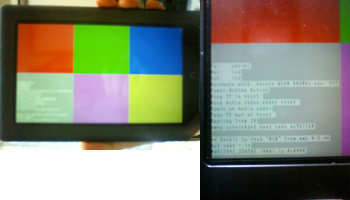
\includegraphics[width=1\hsize]{image2012-gum/u-boot-nook.png}
  \end{center}
  \caption{U-Boot$B$,5/F0$7$F$$$kMM;R(B}
  \label{fig:u-boot-booting}
\end{figure}

$B$J$*!"$3$3$G>R2p$9$k(BU-Boot$B$N2~B$$O!"$^$@IT==J,$J$?$a!"B3$/(BuImage$B$r(Bmini-SD$B$+$i(B
$B%m!<%I$7$F%+!<%M%k$r<B:]$KN)$A>e$2$k$H$3$m$^$G$O=PMh$F$$$^$;$s!#$7$+$7$J$,$i!"(B
U-Boot$B$N(Bprintf()$B$K5-:\$7$?7k2L$O(BLCD$B$K=PNO$G$-$F$$$k$N$G!"$3$A$i$r(B
$B85$K(BU-Boot$B$N2~B$$rB3$1$k;v$,$G$-$=$&$G$9!#(B

\subsection{$B=*$o$j$K(B}

$B:#2s%V!<%H%m!<%@$G$"$k(BU-Boot$B$r;H$$!"(BDebian$B>e$G%/%m%9%3%s%Q%$%k4D6-$r:n$C$F(B
$B<B:]$K(BU-Boot$B$,5/F0$9$k$^$G;n$7$F$_$^$7$?!#(BPC$B$[$I$K$O(BBIOS$B$bL5$$!"%G%P%C%0MQ%]!<%H$bL5$$(B
$B<B4D6-$G!"Bg$7$?2~B$$d;n9T:x8m$b$J$/!"$$$-$J$j(BLCD$B$K(Bprintf()$B=PMh$k$N$O(BU-Boot$B$,(B
$B$h$/$G$-$F$$$k>Z5r$@$H;W$$$^$9!#$^$?!"E,Ev$J<B4D6-$,L5$/$F$b!"(BDebian$B$5$($"$l$P(B
$BAH$_9~$_5!BP1~$N%O%C%/$rM_K>$N$^$^$K;n$9$3$H$b$G$-$^$9!#(B

$B:r:#(BAndroid$BC<Kv$NIa5Z$N$*$+$2$G!"$b$N$9$4$$@*$$$G9+$K!VIT<+M3!W$J%=%U%H%&%'%"4D6-$G(B
$B8G$a$i$l$?(BARM CPU$BEk:\$N>pJsC<Kv$,$"$U$l$F$$$^$9!#$3$l$r$-$C$+$1$K(BDebian$B$r;H$C$F(B
$B$3$l$i$NC<Kv$r!V<+M3!W$J%=%U%H%&%'%"4D6-$XJQ$($F$F$_$^$;$s$+!)(B

\begin{thebibliography}{0}

\bibitem{u-boothistory} 
U-bootdoc 1.2 History,
\url{http://www.denx.de/wiki/view/U-Bootdoc/History}

\bibitem{qemu-u-boot}
Virtual Development Board,
\url{http://www.elinux.org/Virtual_Development_Board}

\bibitem{android-debian} 
$BEl5~%(%j%"(BDebian$BJY6/2q(B2012$BG/(B4$B7n;qNA(B,
\url{http://tokyodebian.alioth.debian.org/pdf/debianmeetingresume201204.pdf}

\bibitem{orig-kernel-nook}
NookColor: Build the Original Kernel,
 \url{http://nookdevs.com/NookColor:_Build_the_Original_Kernel}

\end{thebibliography}

%------------------------------------------------------------------------------
\dancersection{Debian Multiarch Support}{$B$J$+$*$1$$$9$1(B}
\label{sec:Multiarch}
%------------------------------------------------------------------------------

\subsection{$B$O$8$a$K(B}
Debian Multiarch Support$B$O!"F1$8%7%9%F%`>e$G!"J#?t$N%"!<%-%F%#%/%A%c!<$N%i%$%V%i%j$d%W%m%0%i%`$r%$%s%9%H!<%k$*$h$S<B9T$9$k$7$/$_$G$9!#$^$?%(%_%e%l!<%?$d(Bcross-build$B4D6-$bDs6!$5$l$F$*$j!"(Bamd64$B$H(Barmel$B$N$h$&$KBg$-$/0[$J$C$?%"!<%-%F%#%/%A%c$N%W%m%0%i%`$bF0$+$9$3$H$,$G$-$^$9!#(B

$B$?$H$($P(B64bit$B$N%^%7%s$G!"$"$k%W%m%0%i%`$rF0$+$7$?$$$N$K(B32bit$BHG$7$+$J$$$3$H$,$"$j$^$9!#(Bmultiarch$B$G$O!"$=$N%W%m%0%i%`$,0MB8$7$F$$$k(B32bit$BHG$N%i%$%V%i%j%Q%C%1!<%8$r%$%s%9%H!<%k$9$k$3$H$,$G$-$k$N$G!"(B32bit$BHG$N%W%m%0%i%`$r(B64bit$B4D6-$GF0$+$9$3$H$,$G$-$^$9!#(B
$B$^$?!"(Bx86-64$B$N%G%9%/%H%C%W$G(BARM$B$N%=%U%H%&%'%"$r3+H/$7$?$$$H$-$O!"(Barmel$BHG$N(Bbuild-dependent$B%i%$%V%i%j$r%$%s%9%H!<%k$9$l$P!"(Bx86-64$B$N%G%9%/%H%C%W$G3+H/$9$k$3$H$,$G$-$^$9$7!"(Bqemu$B$r;H$($P!"%F%9%H$9$k$3$H$b$G$-$^$9!#(B

$B$?$@Cm0U$7$J$1$l$P$$$1$J$$$N$O!"J#?t$N%"!<%-%F%#%/%A%c$,6&B8$G$-$k$N$O(B**$B%i%$%V%i%j%Q%C%1!<%8$@$1(B**$B$G!"(B**$B%W%m%0%i%`$O6&B8$G$-$J$$(B**$B$H$$$&$3$H$G$9!#(B


%%%%%%%%%%%%%%%%%%%%%%%%%%%%%%%%%%%%%%%%%%%%%%%%%%%%%%%%%%
%% HOW TO USE MULTIARCH?
%%%%%%%%%%%%%%%%%%%%%%%%%%%%%%%%%%%%%%%%%%%%%%%%%%%%%%%%%%


\subsection{$B$D$+$$$+$?(B}
Multiarch$B$r;H$&$K$O!"%$%s%9%H!<%k$7$?$$B>$N%"!<%-%F%#%/%A%c$r;XDj$7$^$9!#$3$l$r%;%+%s%I%"!<%-%F%#%/%A%c$H8F$S$^$9!#%;%+%s%I%"!<%-%F%#%/%A%c$r;XDj$7$?8e!"I,$:%Q%C%1!<%8%G!<%?%Y!<%9$r99?7$7$F$/$@$5$$!#Nc$($P(Bamd64$B$GF0$$$F$$$k%^%7%s$K!"(Bi386$B$N%Q%C%1!<%8$r%$%s%9%H!<%k$7$?$$>l9g$O0J2<$N$h$&$K$J$j$^$9!#(B

\begin{commandline}
# dpkg --print-architecture  # $B$I$N%"!<%-%F%#%/%A%c!<$G%^%7%s$,F0$$$F$$$k$+I=<((B
amd64
# dpkg --add-architecture i386 # i386$B$rDI2C(B
# dpkg --print-foreign-architectures
i386
# apt-get update # $B%Q%C%1!<%8%G!<%?%Y!<%9$r99?7(B
\end{commandline}

$B$3$3$G!"(Baptitude$B%3%^%s%I$G%Q%C%1!<%8$N%j%9%H$rI=<($9$k$H!"%Q%C%1!<%8L>$N8e$m$K!"(B:i386$B$HI=<($5$l$^$9!#$?$H$($P(Blibc6:i386$B$G$"$l$P!"(Bi386$BMQ$N(Blibc6$B%Q%C%1!<%8$H$$$&0UL#$G$9!#(B

\begin{commandline}
$ aptitude search libc6
i   libc6                           - $BAH9~MQ(B GNU C $B%i%$%V%i%j(B: $B6&M-%i%$%V%i%j(B
p   libc6:i386                      - $BAH9~MQ(B GNU C $B%i%$%V%i%j(B: $B6&M-%i%$%V%i%j(B
p   libc6-amd64:i386                - $BAH9~MQ(B GNU C $B%i%$%V%i%j(B: AMD64 $BMQ(B 64 $B%S%C(B
p   libc6-dbg                       - $BAH9~MQ(B GNU C $B%i%$%V%i%j(B: $BJ,N%$7$?%G%P%C%0(B
p   libc6-dbg:i386                  - $BAH9~MQ(B GNU C $B%i%$%V%i%j(B: $BJ,N%$7$?%G%P%C%0(B
....
\end{commandline}

$B$=$l$G$O!"(Bi386$BHG$N(Blibc6$B%Q%C%1!<%8$r%$%s%9%H!<%k$7$F$_$^$7$g$&!#(B
$BB>$N%"!<%-%F%#%/%A%c!<$N%Q%C%1!<%8$r%$%s%9%H!<%k$9$k$K$O!"(B
\begin{commandline}
# apt-get install package:architecture
\end{commandline}

$B$H;XDj$7$^$9!#$h$C$F(Bi386$BMQ$N(Blibc6$B$r%$%s%9%H!<%k$7$?$$>l9g$O!"0J2<$N$h$&$K$J$j$^$9!#(B

\begin{commandline}
# apt-get install libc6:i386
\end{commandline}


$B$=$l$G$O!"(Bi386$B$N%W%m%0%i%`$,F0$/$+;n$7$F$_$^$7$g$&!#(Bi386$B%"!<%-%F%#%/%A%c$GF0$$$F$$$k%^%7%s$G!"0J2<$N%W%m%0%i%`$r%3%s%Q%$%k$7$^$9!#(B
\begin{commandline}
$ uname --machine
i686

$ cat hello.c
#include <stdio.h>
#include <sys/utsname.h>

int main(void)
{
	struct utsname u;
	if(-1 == uname(&u)){
		perror("uname");
		return -1;
	}

	printf("Hello World on %s\n", u.machine);
	return 0;
}

$ gcc -o hello-i686 hello.c

$ file hello-i686
hello-i686: ELF 32-bit LSB executable, Intel 80386, version 1 (SYSV), dynamically linked (uses shared libs),
for GNU/Linux 2.6.18, not stripped

$ ./hello-i686
Hello World on i686
\end{commandline}
%$

32bit ELF$B$N%P%$%J%j$,$G$-$F!"(Bi386$B%"!<%-%F%#%/%A%c$N>e$GF0$/%W%m%0%i%`$H$$$&$3$H$,$o$+$j$^$9!#$3$l$r!"(B{\tt libc6:i386}$B$,%$%s%9%H!<%k$5$l$?(Bamd64$B$GF0$$$F$$$k%^%7%s$K$K%3%T!<$7$F!"<B9T$G$-$k$+;n$7$F$_$^$7$g$&!#(B

\begin{commandline}
$ uname --machine
x86_64

$ ./hello-i686
Hello World on x86_64

$ file hello-i686
hello-i686: ELF 32-bit LSB executable, Intel 80386, version 1 (SYSV), dynamically linked (uses shared libs),
for GNU/Linux 2.6.18, BuildID[sha1]=0x2898c6a77a71f4ae529ae4fb7f91beff44f6762e, not stripped
\end{commandline}
%$
$B$9$P$i$7$$!#(Bhello-i686$B$O!"(BELF 32bit$B%P%$%J%j$K$b$+$+$o$i$:(Bamd64$B$N%^%7%s$G$A$c$s$HF0$$$F$$$^$9!#$G$b$J$<$3$s$J$3$H$,$G$-$k$N$G$7$g$&!#(B

\subsection{Mulit-Arch $B$N$7$/$_(B}
Linux$B$O!"<B9T%U%!%$%k%U%)!<%^%C%H$K!"(BELF(Executable and Linkable Format)$B$r:NMQ$7$F$$$^$9!#$"$k%W%m%0%i%`$,<B9T$5$l$k$H$-!"$^$:<B9T%U%!%$%k$N%X%C%@$K$"$k!"(B{\tt PT\_INTERP}$B$G;XDj$5$l$F$$$k(BELF$B%$%s%?!<%W%j%?$,%m!<%I$5$l$^$9!#(BELF$B%$%s%?!<%W%j%?$O!"%W%m%0%i%`$N<B9T$KI,MW$J%@%$%J%_%C%/%i%$%V%i%j$r%m!<%I$7$^$9!#$3$N$H$-!"(Bglibc$B$O!"(B-rpath$B$d!"4D6-JQ?t(B{\tt LD\_LIBRARY\_PATH}$B!"%O!<%I%3!<%I$5$l$?%G%#%l%/%H%j$J$I$r$^$o$C$FI,MW$J%i%$%V%i%j$rC5$7$^$9!#(B

multiarch$B$O!"%7%9%F%`>e$GMxMQ2DG=$J$?$/$5$s$N%i%$%V%i%j$NCf$+$i:GE,$J$b$N$r<+F0E*$KA*Br$9$k!"$3$N$7$/$_$r;H$C$F<B8=$5$l$F$$$^$9!#$9$J$o$A!"%"!<%-%F%#%/%A%cKh$K7h$^$C$?%G%#%l%/%H%j$K%i%$%V%i%j$r%$%s%9%H!<%k$7$F!"(Bglibc$B$,8!:w$9$k%G%#%l%/%H%j$N%j%9%H$K$=$l$i$N%G%#%l%/%H%j$rDI2C$7$F$*$1$P!"<+F0E*$KI,MW$J%i%$%V%i%j$rA*$s$G$/$l$k$H$$$&$o$1$G$9!#(B

%$B%i%$%V%i%j$,%$%s%9%H!<%k$5$l$k%G%#%l%/%H%j$O!"0J2<$N$H$*$j$G$9!#(B
%\begin{itemize}
%\item /lib/\$(biarch\_suffix)
%\item /usr/lib/\$(biarch\_suffix)
%\end{itemize}

$B$?$H$($P!"(B{\tt libc6:i386}$B%Q%C%1!<%8$NCf?H$r8+$F$_$k$H!"6&M-%i%$%V%i%j$,(B{\tt /lib}$B$G$O$J$/!"(B{\tt /lib/i386-linux/gnu}$B$K%$%s%9%H!<%k$5$l$F$$$k$3$H$,$o$+$j$^$9!#(Bmultiarch$B$KBP1~$7$?%i%$%V%i%j%Q%C%1!<%8$O!"0JA0$N$h$&$KLdEzL5MQ$G(B{\tt /lib}$B$d(B{\tt /usr/lib}$B$KF~$l$k$N$G$O$J$/!"(B{\tt /lib/i386-linux-gnu}$B$d!"(B{\tt /usr/lib/i386-linux-gnu}$B$K%$%s%9%H!<%k$5$l$F$$$k$3$H$,$o$+$j$^$9!#(B

\begin{commandline}
$ dpkg -L libc6:i386
/.
/lib/i386-linux-gnu/libnss\_nis-2.13.so
/lib/i386-linux-gnu/libpthread-2.13.so
....(snip)

/etc/ld.so.conf.d
/etc/ld.so.conf.d/i486-linux-gnu.conf
....(snip)

/usr/lib/i386-linux-gnu/gconv/EUC-JISX0213.so
/usr/lib/i386-linux-gnu/gconv/KOI8-T.so
/usr/lib/i386-linux-gnu/gconv/IBM1144.so
....(snip)

/lib/ld-linux.so.2
/lib/i386-linux-gnu/libnss\_nis.so.2
/lib/i386-linux-gnu/libthread_db.so.1
....(snip)
\end{commandline}
%$
$B@h$[$I$N(Bhello-i686$B$,%m!<%I$7$F$$$k%i%$%V%i%j$rD4$Y$F$_$k$H!"0J2<$N$h$&$K$J$j!"(B
$B<B9T;~$K%j%s%/$5$l$k6&M-%i%$%V%i%j$,!"(B{\tt /lib/i386-linux-gnu}$B$J$I$+$i%m!<%I$5$l$F$$$k$3$H$,$o$+$j$^$9!#(B
\begin{commandline}
$ ldd hello-i686
	linux-gate.so.1 =>  (0xf76e3000)
	libc.so.6 => /lib/i386-linux-gnu/i686/cmov/libc.so.6 (0xf756d000)
	/lib/ld-linux.so.2 (0xf76e4000)
\end{commandline}
%$


%%%%%%%%%%%%%%%%%%%%%%%%%%%%%%%%%%%%%%%%%%%%%%
%% HOW TO CONVERT TO MULTIARCHED PACKAGE
%%%%%%%%%%%%%%%%%%%%%%%%%%%%%%%%%%%%%%%%%%%%%%

\subsection{$B6&M-%i%$%V%i%j%Q%C%1!<%8$r!"(BMultiarch$BBP1~$K$9$kJ}K!(B}
\subsubsection{$B%i%$%V%i%j$r%$%s%9%H!<%k$9$k%G%#%l%/%H%j(B}
multiarch$BBP1~%Q%C%1!<%8$X$NJQ49J}K!$O!"(BDebian Wiki$B$N(BUsing multiarch\footnote{\url{http://wiki.debian.org/Multiarch/Implementation}}$B$K>\$7$/=R$Y$i$l$F$$$^$9!#(B
Debian Policy (9.1.1)\footnote{\url{http://www.debian.org/doc/debian-policy/ch-opersys.html\#s-fhs}}$B$G!"(Bmultiarch$B$K4X$9$k$3$H$O6&M-%i%$%V%i%j$N(BPATH$B$7$+Dj5A$5$l$F$$$^$;$s!#0lJ}$G(B(autoconf$B$N$h$&$J(B)$B$[$H$s$I$N%"%C%W%9%H%j!<%`$N%S%k%I%7%9%F%`$O!"6&M-%i%$%V%i%j$d!"%5%]!<%H%U%!%$%k!"(B(static $B%i%$%V%i%j$d(B.so$B%U%!%$%k$N%7%s%\%j%C%/%j%s%/$N$h$&$J(B)$B3+H/$K;H$&%U%!%$%k$rF1$8%?!<%2%C%H%G%#%l%/%H%j$K%$%s%9%H!<%k$7$h$&$H$7$^$9!#(BDebian Policy$B$O$3$N$h$&$J%U%!%$%k$r$9$Y$F!"(B/usr/lib/{\it triplet}$B%5%V%G%#%l%/%H%j$K%$%s%9%H!<%k$G$-$k$h$&$KJQ99$5$l$kM=Dj$G$9!#(B
$B$3$3$G(B{\it triplet}$B$H$O!"(B{\tt dpkg-architecture -qDEB\_HOST\_MULTIARCH}$B%3%^%s%I$,JV$9CM$N$3$H$G$9!#(B
multiarch$B$G$O!"%i%$%V%i%j$d<B9T%P%$%J%j$r%$%s%9%H!<%k$9$k%G%#%l%/%H%j$O!"$3$N$h$&$KJQ99$5$l$^$9!#(B
\begin{commandline}
/usr/lib -> /usr/lib/<triplet>
/usr/lib/<pkgdir> -> /usr/lib/<triplet>/<pkgdir>
/usr/include: no change
/usr/bin: no change
/usr/share: no change
/usr/sbin: no change
\end{commandline}

\subsubsection{$B%Q%C%1!<%8%U%#!<%k%I(B: Multi-Arch}
multiarch$B$,F3F~$5$l$kA0$O!"%Q%C%1!<%8$N0MB84X78$O!"F1$8%"!<%-%F%#%/%A%c$+!"$9$Y$F$N%"!<%-%F%#%/%A%c$r%5%]!<%H$7$F$$$k%Q%C%1!<%8$r;H$C$F$G2r7h$5$l$F$$$^$7$?!#F1$8L>A0$G0[$J$k%"!<%-%F%#%/%A%c$N%Q%C%1!<%8$OEvA3F1;~$K%$%s%9%H!<%k$G$-$J$$$b$N$H07$o$l$F$$$^$7$?!#(Bmultiarch$B$N;EMM$G$O!"(B{\tt Multi-Arch}$B$H$$$&?7$7$$%P%$%J%j%Q%C%1!<%8%U%#!<%k%I$rDI2C$7$^$7$?!#$3$N%U%#!<%k%I$O!"(B{\tt same}$B!"(B{\tt foreign}$B!"(B{\tt allowed}$B$N(B3$B$D$NCM$N(B1$B$D$r$H$k$3$H$,$G$-$^$9!#(B

{\tt Multi-Arch:same}$B$N;~$O!"F1$8L>A0$N%Q%C%1!<%8$HF1$8%7%9%F%`$K%$%s%9%H!<%k$9$k$3$H$,$G$-$^$9(B(co-installable)$B$,!"B>$N%"!<%-%F%#%/%A%c$N$"$i$f$k%Q%C%1!<%8$N0MB8$r2r7h$9$k$3$H$K;H$C$F$O$J$i$J$$$3$H$r0UL#$7$F$$$^$9!#$^$?!"(B{\tt Multi-Arch:foreign}$B$N;~$O!"F1$8L>A0$N%Q%C%1!<%8$OF1$8%7%9%F%`$K%$%s%9%H!<%k$9$k$3$H$O$G$-$^$;$s$,!"B>$N%"!<%-%F%#%/%A%c$N%Q%C%1!<%8$N0MB8$N2r7h$K;H$&$3$H$,$G$-$^$9!#(B
$B$D$^$j!"$"$k%i%$%V%i%j$N%"!<%-%F%#%/%A%c!<$K0MB8$9$kItJ,$O!"(B{\tt Multi-Arch:same}$B$N%U%#!<%k%I$r;}$D!"(B{\tt libfoo}$B$H$$$&%Q%C%1!<%8$K$7$F!"%"!<%-%F%#%/%A%c$K0MB8$7$J$$%5%]!<%H%U%!%$%k$J$I$O!"(B{\tt Multi-Arch:foreign}$B$NCM$r;}$D!"$?$H$($P(B{\tt libfoo-data}$B$H$$$&%Q%C%1!<%8$KJ,N%$9$kI,MW$,$"$j$^$9!#(B
$B:G8e$N(B{\tt Multi-Arch:allow}$B$O!"(Breverse-dependency$B$,$"$k%Q%C%1!<%8$G!"F1$8L>A0$NB>$N%"!<%-%F%#%/%A%c$N%Q%C%1!<%8$,0MB8$r2r7h$G$-$k$H$-$K;XDj$7$^$9!#$3$l$O!"0MB8$7$F$$$k%Q%C%1!<%8$N%a%s%F%J$NCg2p$J$7$K!"%Q%C%1!<%8$,%"!<%-%F%#%/%A%c$K4X78$7$J$$0MB8$r;}$D$H!"8m$C$FI=L@$9$k$3$H$rKI$0$?$a$K$"$j$^$9!#(B

\subsubsection{multiarch$BBP1~%Q%C%1!<%8$r:n@.$9$k<j=g(B}
autoconf$B$r;H$C$?(Bupstream$B$N%=!<%9$r(Bdh$B$r;H$C$F!"4JC1$J%Q%C%1!<%8$r(Bmultiarch$B$KBP1~$5$;$k$H$-$N<j=g$O!"$3$N$h$&$K$J$k$G$7$g$&!#(B
\begin{enumerate}
\item debhelper($>=9$)$B$K(BBuild-depend$B$5$;$k(B
\item {\tt Pre-Depends:\$\{misc:Pre-Depends\}}$B$rDI2C$9$k(B
\item {\tt debian/compat}$B$r(B9$B$K$9$k(B
\item {\tt debian/*.install}$B$NCf$N(B{\tt /usr/lib}$B$r!"(B{\tt /usr/lib/*/}$B$KJQ99$9$k(B
\item $B$b$7(B{\tt debian/*.install}$B$d!"(B{\tt debian/*.link}$B$G!"(B{\tt /usr/lib}($B$^$?$O$=$N%5%V%G%#%l%/%H%j(B)$B$K%$%s%9%H!<%k$5$l$k%U%!%$%k$r;XDj$7$F$$$k!"$b$7$/$O%j%s%/$rD%$k$h$&$K;XDj$7$F$$$k$J$i!"(B{\tt debian/rules}$B$G!"(B{\tt \$(DEB\_HOST\_MULTIARCH)}$B$NCM$r;H$&$h$&$KJQ99$7$?!"$3$l$i$N%U%!%$%k$r<+F0@8@.$9$kI,MW$,$"$k$G$7$g$&!#(B
\item {\tt debian/rules}$B$NCf$K5-=R$5$l$F$$$k!"(B{\tt /usr/lib}$B$r$9$Y$F(B{\tt /usr/lib/\$(DEB\_HOST\_MULTIARCH)}$B$KJQ99$9$k(B
\item {\tt debian/rules}$B$NCf$GJQ?t(B{\tt \$(DEB\_HOST\_MULTIARCH)}$B$r;H$&I,MW$,$"$k$N$J$i!"(B{\tt debian/rules}$B$NCf$K!"(B{\tt DEB\_HOST\_MULTIARCH ?= \$(shell dpkg-architecture -dDEB\_HOST\_MULTIARCH)}$B$H5-=R$7$F!"JQ?t(B{\tt DEB\_HOST\_MULTIARCH}$B$r=i4|2=$9$k!#(B
\item $B%Q%C%1!<%8$,%S%k%I$G$-$F!"6&M-%i%$%V%i%j%Q%C%1!<%8$K!";W$C$?$H$*$j$N%U%!%$%k$@$14^$^$l$F$*$j!"(B-dev$B%Q%C%1!<%8$b$-$A$s$HF0:n$9$k$3$H$r3N$+$a$?$i!"(B{\tt Multi-Arch: same}$B$H!"(Bdebian/contorl$B$K5-=R$9$k!#(B
\item (architecture: all $B$N(B)common$B%Q%C%1!<%8$,I,MW$J$i!"(B{\tt debian/control}$B$G!"(Bcommon$B%Q%C%1!<%8$K!"(B{\tt Multi-Arch:foreign}$B$H@_Dj$9$k!#(B
\end{enumerate}


\subsection{$B$^$H$a(B}
Debian multiarch$B$O!"(B1$B$D$N%7%9%F%`$KJ#?t$N%"!<%-%F%#%/%A%c$N%i%$%V%i%j!"%W%m%0%i%`$r%$%s%9%H!<%k!"<B9T$9$k$?$a$N$7$/$_$G$9!#$3$NJ8=q$G$O!"(Bmultiarch$B$N;H$$J}$H!"$7$/$_!"(Bmultiarch$B$KBP1~$7$?6&M-%i%$%V%i%j%Q%C%1!<%8$N:n@.J}K!$r@bL@$7$^$7$?!#(Bmultiarch$B$O!"(Bwheezy$B$N(BRelease Goal$B$G$9!#<!4|%j%j!<%9$G$O$9$Y$F$N$R$H$,!"(BDebian multiarch$B$r;H$&$3$H$,$G$-$^$9!#(B

\begin{thebibliography}{8}
\bibitem{spec} MultiarchSpec \url{https://wiki.ubuntu.com/MultiarchSpec}
\bibitem{impl} Multiarch Implementation \url{http://wiki.debian.org/Multiarch/Implementation}
\bibitem{toolchain} Multiarch paths and toolchain implications \url{http://wiki.debian.org/Multiarch/LibraryPathOverview}
\end{thebibliography}


%------------------------------------------------------------------------------
\dancersection{$B2HDmFb(BLAN$B$r9bB.$K!*(B - InfiniBand on Debian}{$B;3ED(B $BBY;q(B}
\label{sec:ibdebian}
%------------------------------------------------------------------------------

$B:G6a$N(BInfiniBand(IB)\cite{IBSPEC}$B5!:`$N0B$5$K!";W$o$:2HDmFb(BIB$B$K(B
$B<j$r=P$7$F$7$^$$$^$7$?!#$=$NF3F~7P83$rJs9p$7$^$9!#(B

\subsection{InfiniBand$B$NFCD'$HA4BNA|(B}
$B:G=i$K(BIB$B$K?($l$F8MOG$&$N$O!"5,Dj$5$l$F$$$kHO0O$,(BL1-L7$B$HI}9-$/!"(B
$B47$l?F$7$s$G$-$?(BL2:Ethernet$B!"(BL3:IP$B!"!D$H$$$&3,AX9=B$$K<}$^$k(B
$BC1$J$k!V?7$7$$(BL2$B5,3J!W$G$O$J$$$3$H$G$9!#$^$?!"MQ8l$NEP>l6q9g$,(B
\begin{screen}
IB$B$N(BL4$B$K$"$?$kItJ,$K$O(BRC/RD/UC/UD/XRC$B$J$I$,$"$j$^$9!#(B
RC$B$,(BTCP$B!"(BUD$B$,(BUDP$B$KAjEv$7$^$9!#(BIP$B$d(BMAC$B$KBP1~$9$kMWAG$,(BGID/LID$B!"(B
$B%]!<%H$KAjEv$9$kMWAG$O(BQP$B$H$$$&N>C<$N(BHCA$B>e$K3NJ]$5$l$k%-%e!<(B(WQ)$B$N(B
$BAH$H8@$($^$9!#$=$7$F(BWQ$B$,(B1$BBP(B1$BBP1~$9$k7A$G(BQP$B$r7A@.$9$k$b$N$,(BRC/UC$B!"(B
1$BBP(BN$BBP1~$9$k7A$N$b$N$,(BRD/UD/XRC$B$H$$$&J,N`$K$J$j$^$9!#(BSRP$B$J$I$N(B
ULP$B$O(BWQ$B$K3F<o(BVerb$B$r(BWQE$B$N7A$GAw$j9~$_!"(BHCA$B$r6nF0$7$F(BRDMA$B$rMxMQ$7$F$$$^$9!#(B
\end{screen}
$B$J$I$H(BTLA$B$,J,Ln2#CG$+$D5M$a9~$_5$L#$J$N$KG:$^$5$l$^$9(B
\footnote{$B$3$l$O3F<o;qNA$ND4;R$rLO$7$F5M$a9~$s$G$_$?%5%s%W%k$G$9!#%;%C%7%g%s$G$O>e5-FbMF$O?^$G2r@bM=Dj(B}
$B!#(B

$B;fLL$N4X78$+$i>\$7$/$O%9%i%$%I$G$H$J$j$^$9$,!";qNA$rFI$`>e$G$OGX7J$H$7$F(B
\begin{itemize}
\item RDMA$B$N$?$a(BOS$B%P%$%Q%9$,I,MW$H$J$j!"@0M}!&5,DjHO0O$,(BL7$B$^$G5Z$V$3$H(B
\item $B4{B8%l%$%d$X$N(BRDMA$BF3F~$N$?$a35G0!\5,3J!\(BAPI$B$H@0M}$,:Y$+$/$J$C$F$$$k$3$H(B
\item L2-L3$BAjEv$NMWAG$K$O(BIB/RoCE/iWARP$B$N;0<o$,$"$j!"(BVerbs$B$GCj>]2=$5$l$k$3$H(B
\end{itemize}
$B$H$$$&E@$^$G$r2!$5$($?>e$G!"F1$8(BIB$B$G$b$I$N%l%$%d0LCV$NOC$J$N$+!"(B
$B$^$?!"K\Ev$N0UL#$G(BIB$B8GM-$J$N$+(BRDMA$B7O3F<o5,3J$KE,MQ$G$-$kOC$+$r(B
$B9M$($J$,$iFI$_?J$a$k$H:.Mp$7$K$/$/$J$j$^$9!#(B

\subsection{InfiniBand on Debian$B$N8=>u(B}
$B%W%m%H%3%k%9%?%C%/$d%I%i%$%P$OAG$N(BLinux kernel$B$K$b35$MF~$C$F$$$k$N(B
$B$G$9$,!"4IM}%D!<%k$J$I$b4^$a$?7A$G$O(BOFA$B$,(BOFED(OpenFabrics Enterprise
Distribution)$B$r3+H/!&G[I[$7$F$$$^$9!#(BOFED$B$N(BLinux$BHG$O(BRedHat$B8~$1$G$9$,!"(B
$B<B:]$K$O$3$l$r85$K3F<R$,0\?"!&FH<+3HD%$r9T$C$?$b$N$r:FG[I[$7$F$*$j!"(B
$BM-NO$J$b$N$K(BMellanox$B<R$N(BMLNX\_OFED$B%Q%C%1!<%8$,$"$j$^$9(B
\footnote{
$B$3$l$NIUB0%^%K%e%"%k(B\cite{MLNXMAN}$B$O2?$rA<$$$F$bFI$`$Y$-;qNA(B
}$B!#(B

Debian$B$G$O(BOFED Infiniband Distribution project
\footnote{http://pkg-ofed.alioth.debian.org/}
$B$,%I%-%e%a%s%H@0Hw$H%Q%C%1!<%8%s%0$r9T$C$F$*$j!"(Bsqueeze$B8~$1$K$O(B
OFED-1.4.2$B$,!"$=$7$F(Bwheezy/sid$B8~$1$K(BOFED-1.5$B$N%Q%C%1!<%8%s%0$,(B
$BCY$l5$L#$G$9$,?J$s$G$$$^$9!#%W%m%8%'%/%H%Z!<%8$K$O(B
\begin{commandline}
deb     http://pkg-ofed.alioth.debian.org/apt/ofed-X.Y.Z ./
deb-src http://pkg-ofed.alioth.debian.org/apt/ofed-X.Y.Z ./
\end{commandline}
$B$N(Bapt-line$B$rDI2C$7$?>e$G(B apt-get install ofed $B$GF~$k$H$"$j$^$9$,!"(B
$B$3$3$K$O(B1.4.2$B$^$G$7$+$J$$$?$a!"8=>u$G$O(Bwheezy/sid$B$+$i@h<h$j$9$k$+(B
$B<+J,$G%S%k%I$7$^$9(B\footnote{$B0J9_$N@bL@$O(Bsid$B4D6-!"$^$?!">R2p$9$k(B
$B5!G=$N4X78$G(BLinux 3.4.0$B%Y!<%9$H$J$j$^$9(B}$B!#(B

$B:#2s%l%Y%k$G;H$&J,$K$O(BOFED-1.4$B$GLdBj$J$$$N$G$9$,!"Nc$($P(BIB-FDR
\footnote{IB$B$O%7%j%"%k%j%s%/$rB+$M$kJ}<0$G!"%j%s%/Ev$?$jB.EY$r(B
SDR(2Gbps), DDR(4Gbps), QDR(8Gbps), FDR(14Gbps), EDR(26Gbps), ...$B$H(B
$B9bB.2=$7$FBS0h$rA}$d$7$^$9!#$^$?%j%s%/?t$b(Bx1, x4, x12$B$,(B
$B5,Dj$5$l$F$$$^$9!J(Bx4$B$N%?%$%W$,<gN.!K(B}
$B$X$NBP1~$O(B1.5.4$B0J9_$,I,MW$K$J$j!"$^$?!"$5$i$K?7$7$$5!G=$d%+!<%M%k$r(B
$B;H$&$N$G$"$l$P(BOFED-3.2$B$d3+H/Cf%j%]%8%H%j(B
\footnote{https://beany.openfabrics.org/downloads/MAINTAINERS}
$B%Y!<%9$G$N%j%S%k%I$,I,MW$K$J$k$J$I!";n9T:x8m$,I,MW$G$9!#(B

\subsection{$B;H$C$F$_$h$&(B - $B4pK\E*$J(BIB/IPoIB$B4D6-$N9=C[(B}
$B$=$l$G$O;H$C$F$_$^$7$g$&!#4pK\E*$JItJ,$K$D$$$F$O@h$N(BDebian$B$N(B
$B%W%m%8%'%/%H;qNA(B\cite{DEBIANIB}$B$d3F<o$NF|K\8l5-;v(B\cite{ALTIMA}
\cite{ATMARK}$B$b$"$k$?$a!"8=:_(BDebian$B$G9=C[$9$k$K$"$?$j8GM-$N(B
$BItJ,$@$1$r>R2p$7$^$9!#(B

\subsubsection{$B%Q%C%1!<%8$NF3F~$H=i4|%;%C%H%"%C%W(B}
$B%W%m%8%'%/%H$N%j%]%8%H%j$G$"$l$P(Bofed$B%Q%C%1!<%8$,$"$k$N$G$9$,!"(B
$B$3$l$O8=>u(Bbroken dependency$B$N>uBV$N$?$a!"(Bsid$B$NJ}$h$j8DJL$KF3F~$7$^$9!'(B


\begin{commandline}
# apt-get install opensm ibverbs-utils infiniband-diags perftest                     // $B4pK\%D!<%k72(B
# apt-get install libmlx4-1 libmthca1 mstflint                                       // HCA$B4X78%Q%C%1!<%872(B
# apt-get install ibutils rdmacm-utils rds-tools libsdp1 dapl2-utils                 // $BDI2C%D!<%k72(B
# apt-get install libibumad-dev libibverbs-dev librdmacm-dev libibcm-dev libdapl-dev // $B3+H/%i%$%V%i%j72(B
\end{commandline}
%$

$B$5$F!"$3$l$G%$%s%9%H!<%k$O$5$l$^$7$?$,!"$3$N$^$^$G$O;H$($^$;$s!#(B
$B$I$N$h$&$J(BULP$B!"Nc$($P(BIPoIB$B$r;H$&$N$+$I$&$+!"$^$?%f!<%6!<%i%s%I$+$i(B
RDMA$B$rC!$/;H$$J}$r$9$k$N$+$J$I$OF3F~%]%j%7<!Bh$J$N$G!"L@<(E*$K(B
$BM-8z2=$9$kI,MW$,$"$j$^$9!#(B

$BAG$N(BOFED$B$K$O$3$l$K;H$($k(Binit$B%9%/%j%W%H(B(openibd.conf + openibd)$B$,(B
$BF~$C$F$$$k$N$G$9$,!"$d$C$F$$$k$3$H$O%b%8%e!<%k%m!<%I$H(Bsysctl$BEy$N(B
$B%Q%i%a!<%?@_Dj$J$N$G!"0J2<$N%b%8%e!<%k$r(B/etc/module$B$KD>@\%m!<%I$7$F(B
$BBe$($k$3$H$,$G$-$^$9!'(B

\begin{commandline}
# Mellanox HCA$B%Y!<%9$G9=C[$7$F$$$k:#2s$N>l9g$N%b%8%e!<%k%j%9%H(B
mlx4_ib ib_mthca ib_uverbs ib_umad ib_ucm rdma_ucm ib_ipoib ib_sdp ib_srp
\end{commandline}
%$

\subsubsection{$B%5%V%M%C%H%^%M!<%8%c$N2TF0(B}
$B%5%V%M%C%H%^%M!<%8%c(B(SM)$B$O7OFb$N%H%]%m%8$r0l854IM}$7!"$^$?(B
$B3F%]!<%H$K(BGID/LID$B$r3d$jEv$F$F(BActive$B>uBV$K$9$k>e$GI,?\$N%5!<%S%9$G$9!#(B
$B%9%$%C%A$KFbB"$5$l$F$$$k$3$H$b$"$j$^$9$,!"J#?t5/F0$7$F$$$F$bLdBj$J$$$?$a(B
$B2<5-$NDL$j5/F0$7$^$9!'(B

\begin{commandline}
# cat /etc/defaults/opensm
PORTS=ALL
# /etc/init.d/opensm start
\end{commandline}
%$

$B8e$O(Bibstat$B$J$I$G%]!<%H>uBV$,(BActive$B$K$J$C$F$$$l$P!"MxMQ2DG=$G$9!#(B

\subsubsection{$B%A%e!<%K%s%0%Q%i%a!<%?(B}
IPoIB$B$N%a%j%C%H$ODL>o$N(BLAN$B%$%s%?%U%'!<%9$H$7$FMxMQ$G$-$k$3$H$G$9$,!"(B
$BH?LL%A%e!<%K%s%0@_Dj$J$7$G$O%*!<%P!<%X%C%I$,Bg$-$/@-G=$,=P$^$;$s!#(B
Mellanox$B$N%,%$%I$K$b$"$j$^$9$,!"0J2<$N@_Dj$O$[$H$s$II,?\$H$J$j$^$9!'(B

\begin{commandline}
# echo connected > /sys/class/net/ib1/mode $B"+(B RC$B%b!<%I$K$7!"(B64KB MTU$B@_Dj$r2DG=$K$9$k(B
# ip link set ib1 mtu 65520                $B"+(B $BF1>e(B
# cat <<EOF > /etc/sysctl.d/network.conf   $B"+(B IB$B$X$N%^%C%T%s%08zN($,8~>e$9$k$h$&!"%P%C%U%!$rBg7?2=$9$k(B
net.ipv4.tcp_timestamps = 0
net.ipv4.tcp_sack = 0
net.core.netdev_max_backlog = 250000
net.core.rmem_max = 16777216
net.core.wmem_max = 16777216
net.core.rmem_default = 16777216
net.core.wmem_default = 16777216
net.core.optmem_max = 16777216
net.ipv4.tcp_mem = 16777216 16777216 16777216
net.ipv4.tcp_rmem = 4096 87380 16777216
net.ipv4.tcp_wmem = 4096 65536 16777216
EOF
# sysctl -qp/etc/sysctl.d/network.conf
\end{commandline}
%$

IP$B%"%I%l%9$N@_Dj$r=*$($?$i!":G8e$KB->l$N3NG'$H$7$F(Bnetperf$B$d(B
ib\_read\_bw$B$K$F@-G=$r3NG'$7$^$7$g$&!#$[$\%o%$%d%l!<%H$,(B
$B=P$;$F$$$l$P:n6H$O40N;$G$9!#(B

\subsection{$B$b$C$H;H$C$F$_$h$&(B - SAN$B9=C[(B}
$B$5$F!"4pK\E*$JF3DL3NG'$O<h$l$?$N$G!"<!$O%5!<%P$H$7$F(BSAN$B$r(B
$B9=C[$7$^$9!#:#2s$O(BiSCSI over IPoIB$B$H(BSRP$B$N(B2$BDL$j$G9T$$!"Hf3S$7$^$9!#(B

\subsubsection{iSCSI over IPoIB}
$B$3$A$i$O(BIPoIB$B$G1#JC$5$l$F$$$k$N$G!"IaDL$N(BiSCSI SAN$B$NF3F~$H<j=g$O(B
$B40A4$KF1$8$G$9!#:#2s$O(B
\begin{itemize}
\item target: Linux-iSCSI (LIO)
\item initiator: open-iscsi
\end{itemize}
$B$NAH$_9g$o$;$G9=C[$7$^$9!#0J2<$,<B:]$N%3%^%s%INc$G$9!#(B

\begin{commandline}
# apt-get install targetcli lio-utils $B"+(B $B%?!<%2%C%HMQ%Q%C%1!<%8$rF3F~(B
# echo 0 $((2 * 1024 * 1024 * 512)) zero | dmsetup create ramdisk $B"+(B $B;n83MQ$K(B512GB$B$N%@%_!<%G%#%9%/$rMQ0U(B
# targetcli
/> cd /backstores/iblock
/backstores/iblock> create ramdisk /dev/mapper/ramdisk $B"+(B $B@h$N%G%#%9%/$rEPO?(B
...
/backstores/iblock/ramdisk> cd /iscsi
\end{commandline}
%$

\begin{commandline}
/iscsi> create iqn.2003-01.org.linux-iscsi:ramdisk $B"+(B IQN$B@8@.(B
...
/iscsi/iqn.20...ramdisk/tpgt1> set attribute authentication=0 $B"+(B $BG'>Z%*%U(B
Parameter authentication is now '0'.
/iscsi/iqn.20...ramdisk/tpgt1> set attribute generate_node_acls=1 $B"+(B $B%"%/%;%9;~$K<+F0E*$K(BACL$B5v2D$r@8@.(B
Parameter generate_node_acls is now '1'.
/iscsi/iqn.20...ramdisk/tpgt1> set attribute demo_mode_write_protect=0 $B"+(B $B=q9~$_J]8n2r=|(B
Parameter demo_mode_write_protect is now '0'.
\end{commandline}
%$

\begin{commandline}
/iscsi/iqn.20...ramdisk/tpgt1> cd luns
/iscsi/iqn.20...sk/tpgt1/luns> create /backstores/iblock/ramdisk 0 $B"+(B $B@h$N%G%#%9%/$rI3IU$1$k(B
...
/iscsi/iqn.20...gt1/luns/lun0> cd ../../portals
/iscsi/iqn.20...tpgt1/portals> create 10.254.1.16      $B"+(B $B%"%/%;%9MQ$N%]!<%?%k$r3+;O(B
...
/iscsi/iqn.20...254.1.16:3260> cd /
/> saveconfig                                          $B"+(B $B:G8e$KJ]B8(B
\end{commandline}
%$

$BC8!9$H%3%^%s%I$rBG$D$@$1$G$7$?$,!"0J>e$G@_Dj$O40N;$G$9!#(B

$B%?!<%2%C%HB&$O$3$l$G2TF0$r;O$a$?$N$G!"<!$O%$%K%7%(!<%?B&$G$9!#(B
open-iscsi$B%G!<%b%s!J(Biscsid$B!K$rF3F~!&5/F0$7$?>e$G!"(Biscsiadm $B%3%^%s%I$G(B
$B%?!<%2%C%HB&$r>H2q$7!"%(%/%9%]!<%H$5$l$F$$$k%9%H%l!<%8$K%"%?%C%A$7$^$9!#(B

\begin{commandline}
# apt-get install open-iscsi
# /etc/init.d/open-iscsi start                               $B"+(B iscsid$B5/F0(B
# iscsiadm -m discovery -t sendtargets -p 10.254.1.16        $B"+(B $B%?!<%2%C%H(BIQN$B$r>H2q$9$k(B
10.254.1.16:3260,1 iqn.2003-01.org.linux-iscsi:ramdisk
# iscsiadm -m node -T iqn.2003-01.org.linux-iscsi:ramdisk -l $B"+(B $B%;%C%7%g%s$r3NN)(B
...
# iscsiadm -m session                                        $B"+(B $BG'<17k2L$r3NG'(B
tcp: [1] 10.254.1.16:3260,1 iqn.2003-01.org.linux-iscsi:ramdisk
# dmesg
...
[ 1403.238057] scsi6 : iSCSI Initiator over TCP/IP
[ 1403.551708] scsi 6:0:0:0: Direct-Access     LIO-ORG  IBLOCK           4.0  PQ: 0 ANSI: 5
...
[ 1404.067053] sd 6:0:0:0: [sde] Attached SCSI disk
\end{commandline}

$B$5$F!"@-G=$O$I$s$J$b$N$G$7$g$&$+!)(B

\begin{commandline}
# JOBS=4 OP=write DEV=/dev/sde BS=1m fio bench.ini
...
Run status group 0 (all jobs):
  WRITE: io=6254.0MB, aggrb=210869KB/s, minb=53870KB/s, maxb=54137KB/s, mint=30287msec, maxt=30370msec
\end{commandline}
%$

$B@5D>$J=j!"$"$^$j?6$k$$$^$;$s!#$5$9$,$K(B200MB/s$B$G$O2~A1$NM>CO$,$"$k$H$O(B
$B;W$o$l$^$9$,!":#2s$N<g4c$O<!$J$N$G$=$N$^$^(BSRP$B$K?J$_$^$9!#(B

\subsubsection{SRP (SCSI RDMA Protocol)}
$B$5$F!"<!$OHf3S$N$?$a(BRDMA$B>e$GD>@\(BSCSI$B$rDs6!$9$k(BSRP$B$G9=C[$7$F$_$^$9!#(B
\begin{itemize}
\item target: SCST (ib\_srpt)
\item initiator: LIO (ib\_srp) $B"+(B $B%+!<%M%kI8=`$N$b$N(B
\end{itemize}
$B$NAH$_9g$o$;$G9=C[$7$^$9!#(BSRP$B$O%?!<%2%C%H!"%$%K%7%(!<%?$NAPJ}$H$b(B
Linux-3.4$B0J9_$N(BLIO$B$K$O4^$^$l$F$$$^$9$,!"%?!<%2%C%H$K$D$$$F$O(BSCST$B$+$i(B
$B%3!<%I$N<h$j9~$_ES>e$GL$=O$J$?$a!":#2s$O(BSCST$B$r;H$C$F$$$^$9!#(B

Debian$B$K$O(BSCST$B$N%Q%C%1!<%8$,$J$$$?$a!"$^$:$O$3$l$N%S%k%I$,I,MW$G$9(B
\footnote{
$B%Q%C%1!<%8$K$7$?$$=j$G$9$,!"$3$l$r%Q%C%1!<%8%s%0$9$k5;NL$,<+J,$K$O$J$$!D(B
}
$B!#(B

\begin{commandline}
$ svn co https://scst.svn.sourceforge.net/svnroot/scst/trunk
$ cd trunk
$ make KDIR=/d/src/linux/master scst iscsi srpt scst_local usr
  ...
  CC [M]  /d/src/scst/trunk/scst/src/scst_main.o
  /d/src/scst/trunk/scst/src/scst_main.c:59:2: warning: #warning
  Patch scst_exec_req_fifo-<kernel-version> was not applied on your kernel.
  Pass-through dev handlers will not work. [-Wcpp]
  ...
make[1]: Leaving directory `/d/src/scst/trunk/usr/fileio'
\end{commandline}
%$

$BA45!G=$r%U%k$K;H$&$K$O%+!<%M%k%Q%C%A$rEv$F$kI,MW$,$"$k$H$$$&7Y9p$,(B
$B2?7o$+=P$^$9$,!":#2s$NL\E*$K$O1F6A$7$J$$$?$a$3$N$^$^?J$_$^$9!#(B
$B:G=*E*$K!"0J2<$N$h$&$J%$%s%9%H!<%k9=@.$K$J$j$^$9!'(B

\begin{commandline}
# ls /var/lib/scst/pr/ <- $B$3$N%U%)%k%@$,$J$$>l9g!":n@.$7$F2<$5$$(B
# ls /lib/modules/3.4.0-rc1-tai-4f7e834f-next-20120405/extra/scst/
 676 ib_srpt.ko        296 scst_disk.ko        300 scst_tape.ko
3712 iscsi-scst.ko     460 scst_local.ko       620 scst_user.ko
4308 scst.ko           296 scst_modisk.ko      704 scst_vdisk.ko
 292 scst_cdrom.ko     272 scst_processor.ko
 272 scst_changer.ko   272 scst_raid.ko
# ls /usr/local/bin/
132 fileio_tgt*   64 iscsi-scst-adm*  372 iscsi-scstd*  152 scstadmin*
\end{commandline}
%$

$B$=$l$G$O(BSCST$B$G(BSRP$B9=@.$r:n$C$F$_$^$7$g$&!#(BiSCSI/LIO$B$N>l9g$O(B
iSCSI daemon$B$r5/F0$7$?>e$G4IM}%3%^%s%I$G@_Dj$rA`:n$9$k7A$G$7$?$,!"(B
SRP$B$N>l9g$O(Bdaemon$B$O$*$i$:!"(Bscstadmin$B%3%^%s%I$G%+!<%M%k%b%8%e!<%k$N(B
$B%m!<%I$H@_Dj$r9T$&$@$1$K$J$j$^$9!#(B

\begin{commandline}
# echo 0 $((2 * 1024 * 1024 * 512)) zero | dmsetup create zero
# cat > scst-test.conf
# $BK\%U%!%$%k$O<jF0:n@.$7$F$b$h$$$,!"(Bscstadmin$B%3%^%s%I$G9=@.$r:n$k7A$G$b$h$$!#(B
# $B0J9_$N%3%a%s%H$G$O@_Dj%(%s%H%j$KBP1~$9$k%3%^%s%INc$r<($9!#(B
#
# CMD: scstadmin -open_dev zero -handler vdisk_blockio --attributes filename=/dev/mapper/zero
HANDLER vdisk_blockio {
        DEVICE zero {
                filename /dev/mapper/zero
        }
}
# CMD: scstadmin -add_lun 0 -driver ib_srpt -target ib_srpt_target_0 -device zero
TARGET_DRIVER ib_srpt {
        TARGET ib_srpt_target_0 {
                enabled 1
                rel_tgt_id 2
                LUN 0 zero
        }
}
^D
# modprobe scst
# modprobe scst_vdisk
# modprobe ib_srpt
# scstadmin -config scst-test.conf
\end{commandline}
%$

$B$3$l$G%?!<%2%C%HB&$O@_Dj40N;$G$9!#<!$O%$%K%7%(!<%?B&$G$9$,!"$3$l$O(B
ibsrpdm$B%3%^%s%I$G%?!<%2%C%HB&$K%/%(%j$rEj$2!"La$C$F$-$?%-!<>pJs$J$I$r(B
ib\_srp.ko$B$K(Bsysfs$B7PM3$G<u$1EO$7$^$9!#(B

\begin{commandline}
# ibsrpdm -c -d /dev/infiniband/umad1
id_ext=0008f1040399d858,ioc_guid=0008f1040399d858,dgid=fe800000000000000008f1040399d85a,pkey=ffff,service_id=0008f1040399d858
# for i in $(ibsrpdm -c -d /dev/infiniband/umad1); do echo $i > /sys/class/infiniband_srp/srp-mlx4_0-2/add_target; done
# dmesg
...
[1493617.766923] scsi8 : SRP.T10:0008F1040399D858
[1493618.663499] scsi 8:0:0:0: Direct-Access     SCST_BIO zero              300 PQ: 0 ANSI: 5
...
[1493620.678542] sd 8:0:0:0: [sdf] Attached SCSI disk
\end{commandline}
%$

$B$H$$$&$o$1$G(BSRP$B$G$bG'<1$G$-$^$7$?!#5/F0;~$K<+F0E*$K%"%?%C%A$5$;$k$K$O!"(B
$B>e5-$N(Bibsrpdm$B=PNO$r(B/etc/srp\_daemon.conf$B$K=q$-9~$_!"5/F0;~$K(Bsrp\_daemon$B$K(B
$BF1MM$N=hM}$r$5$;$k$h$&$K$7$^$9!#(B

$B$5$F!"@-G=$O$I$&$G$7$g$&$+!)(B

\begin{commandline}
# JOBS=4 OP=write DEV=/dev/sdf BS=1m fio bench.ini
...
Run status group 0 (all jobs):
  WRITE: io=26387MB, aggrb=898250KB/s, minb=223059KB/s, maxb=233121KB/s, mint=30048msec, maxt=30081msec
\end{commandline}
%$

$B05E]E*$8$c$J$$$+!"2f$,73$O!&!&!&$H$$$&=j$G$7$g$&$+!#(B
$B%V%m%C%/%5%$%:$,Bg$-$/$J$$$H=P$;$J$$B.EY$J$N$G3d$j0z$$$F(B
$B<u$1<h$kI,MW$O$"$j$^$9$,!"%*!<%P!<%X%C%I$N>/$J$$(BRDMA$B$N0RNO$r(B
$B3@4V8+$k$3$H$,$G$-$^$7$?!#(B

\begin{thebibliography}{0}
\bibitem{IBSPEC} InfiniBandArchitecture Specification Release 1.2.1, \\
\url{http://members.infinibandta.org/kwspub/specs/register/publicspec/}

\bibitem{MLNXMAN} Mellanox OFED for Linux User Manual, \\
\url{http://www.mellanox.com/related-docs/prod\_software/Mellanox%20OFED%20Linux%20User%20Manual%201\_5\_3-3\_0\_0.pdf}

\bibitem{DEBIANIB} Infiniband HOWTO, \\
\url{http://pkg-ofed.alioth.debian.org/howto/infiniband-howto.html}

\bibitem{ALTIMA} Altima - Mellanox $B5;=Q>R2p(B, \\
\url{http://www.altima.co.jp/products/mellanoxtechnologies/mellanox\_techinfo.html}

\bibitem{ATMARK} $B>>K\D>?M(B, InfiniBand$B$GJQ$o$k%G!<%?%;%s%?!<FbDL?.(B, \\
\url{http://www.atmarkit.co.jp/fnetwork/tokusyuu/51ib01/01.html} (2011/2), \\
\url{http://www.atmarkit.co.jp/fnetwork/tokusyuu/61ib02/01.html} (2011/7)

% $B0J2<$N;29MJ88%$OK\J8Cf$KBP1~$9$kFbMF$r@9$j9~$_$-$l$J$+$C$?$?$a%+%C%H(B

% \bibitem{LINUXIB} Bob Woodruff, Sean Hefty, Roland Dreier, and Hal Rosenstock, Introduction to the InfiniBand Core Software, 2005 \\
\url{http://www.kernel.org/doc/ols/2005/ols2005v2-pages-279-290.pdf}

% \bibitem{ITOHRDMA} $B0KF#2mB'(B, $B%W%m%0%i%^L\@~$+$i8+$?(BRDMA$B$N%a%j%C%H$H$=$N1~MQNc$K$D$$$F(B, Nov. 2010 \\
% \url{http://www.slideshare.net/thatsdone/rdma}

% \bibitem{IBHIST} Brief History of InfiniBand: Hype to Pragmatism, \\
% \url{https://blogs.oracle.com/RandomDude/entry/history\_hype\_to\_pragmatism}

% \bibitem{RDMAPROG} RDMA Aware Networks Programming User Manual, \\
% \url{http://www.mellanox.com/related-docs/prod\_software/RDMA\_Aware\_Programming\_user\_manual.pdf}

% \bibitem{RSOCKETS} RSockets, \\
% \url{https://beany.openfabrics.org/ofa-documents/presentations/doc\_download/495-rsockets.html}

% \bibitem{GREGORYAPI} Kerr, Gregory. ``Dissecting a Small InfiniBand Application Using the Verbs API.'', 10 May 2011, \\
% \url{http://arxiv.org/abs/1105.1827}

\end{thebibliography}

\clearpage
\newpage

%------------------------------------------------------------------------------
\dancersection{Gentoo/Prefix on Debian}{$B@DEDD>Bg(B}
\label{sec:gentoo}
%------------------------------------------------------------------------------

\subsection{$B$O$8$a$K(B}

$B$$$-$J$j(BGentoo$B$,=P$F$-$F6C$+$l$?$+$b$7$l$^$;$s!#$3$3$G$O(BDebian$B2<$G(B
Gentoo Prefix$B$r%$%s%9%H!<%k$9$kJ}K!$K$D$$$F2r@b$7$^$9!#(B

\subsection{Gentoo Prefix}
\subsubsection{Gentoo$B$H$O(B}
Gentoo$B$O(BDebian$B$d(BRPM$B$H0c$C$?%=!<%9%Y!<%9$N%G%#%9%H%j%S%e!<%7%g%s$G$9!#(B
ebuild$B$H$$$&%Q%C%1!<%8%S%k%IJ}K!$d!"%Q%C%1!<%8$N0MB84X78$J$I$r5-=R$7$?(B
bash$B%9%/%j%W%HIw$N%U%!%$%k$,(B``$B%+%F%4%j!<(B/$B%Q%C%1!<%8L>(B/$B%Q%C%1!<%8L>(B-$B%Q%C(B
$B%1!<%8%P!<%8%g%s(B.ebuild"$B$H$$$&%U%!%$%kL>$GJ]4I$5$l$F$$$^$9!#(Bemerge$B$H$$(B
$B$&%3%^%s%I$O$3$N(B $B!V(BPortage$B%D%j!<!W$H$$$&%Q%C%1!<%8>pJs%U%!%$%k%D%j!<(B
$B$rFI$s$G;XDj$5$l$?%Q%C%1!<%8$r%S%k%I!&%$%s%9%H!<%k$9$k%Q%C%1!<%84IM}%=%U(B
$B%H$K$J$C$F$$$^$9!#(B

\subsubsection{Prefix$B%5%]!<%H(B}

Gentoo$B$b4pK\E*$K$O(BLinux$B>e$N%G%#%9%H%j%S%e!<%7%g%s$G$9$,!"(BDebian$B$N(B
Debian GNU/kFreeBSD$B$HF1MM$K(BFreeBSD$B>e$G$N%Q%C%1!<%84IM}$rL\E*$H$7$?(B
Gentoo/FreeBSD$B$J$I$N3+H/$b9T$J$o$l$F$$$^$9!#$=$&$$$C$?(BLinux$B0J30$G$N(B
Gentoo$B$N%5%]!<%H$rAm>N$7$F(BGentoo/Alt$B$H8F$s$G$$$^$9!#(B
\footnote{\url{http://www.gentoo.org/proj/en/gentoo-alt/}} $B$=$N(BGentoo/Alt$B$NCf(B
$B$K(BGentoo Prefix$B$H$$$&$b$N$,$"$j$^$9!#(B
\footnote{\url{http://www.gentoo.org/proj/en/gentoo-alt/prefix/index.xml}} $B$3(B
$B$l$O(BGentoo$B$N%7%9%F%`$r;H$C$F(B($B4pK\E*$K$O(B)$BB>$N(BOS$B>e$G!"G$0U$N%G%#%l%/%H%j(B
$B$K%Q%C%1!<%8$N%$%s%9%H!<%k$r9T$J$($k$h$&$K$9$k$b$N$G$9!#$?$H$($P!"(BMac
OS X$B>e$GF0$+$7$F(BMacPorts$B$d(Bhomebrew$B$NBe$o$j$K;H$C$?$j!"$"$k$$$O(B
FreeBSD$B>e$G;H$C$?$j!"$O$?$^$?(BLinux$B>e$G;H$&$3$H$b$b$A$m$s$G$-$^$9!#(B

\subsection{Gentoo/Prefix on Debian}

$B$5$F$3$3$+$i$,K\Bj$G!"$3$N(BGentoo/Prefix$B$r(BDebian$B$G;H$C$F$_$^$9!#$*$=$i$/(B
$B$J$s$G$=$s$J$3$H$r!D(B? $B$H;W$o$l$k$+$b$7$l$^$;$s!#0J2<$N$h$&$JE@$,$"$2$i(B
$B$l$k$+$H;W$$$^$9!#(B

\begin{itemize}
\item $BHs(Broot$B%f!<%6$G$b9%$-$J$H$3$m$K%$%s%9%H!<%k$G$-$k(B
\item Debian$B$K$J$$%Q%C%1!<%8$r%$%s%9%H!<%k$9$k;~$K3Z$G$-$k(B
\item $B5;=QE*$K3Z$7$$(B?
\end{itemize}

Prefix$B%$%s%9%H!<%k$G$O9%$-$J%G%#%l%/%H%j$K%$%s%9%H!<%k$G$-$k$?$a!"$?$H(B
$B$($P<+J,$N%[!<%`%G%#%l%/%H%j$NCf$J$I$K%$%s%9%H!<%k$9$k$h$&$K$7$F$7$^$((B
$B$P(Broot$B8"8B$,$J$/$H$b%Q%C%1!<%8$r%$%s%9%H!<%k$9$k$3$H$,$G$-$^$9!#$^$?!"(B
($B$b$7K|$,0l(B) Debian$B$K$J$$%Q%C%1!<%8$,$"$C$?$H$7$F!"$=$l$,(BGentoo$B$NJ}$K$"(B
$B$l$P!"<+J,$G%S%k%IJ}K!$d0MB8$rD4$Y$k$3$H$J$/!"(BGentoo$B$N%Q%C%1!<%8%7%9%F(B
$B%`$K$*$^$+$;$7$F$7$^$&$3$H$,$G$-$k!"$H$$$&$o$1$G$9!#(B

\subsubsection{$B%$%s%9%H!<%k(B}

$B$G$O!"$5$C$=$/(BDebian$B>e$K%$%s%9%H!<%k$7$F$_$^$7$g$&!#$^$:$O%S%k%I$KI,MW(B
$B$J%Q%C%1!<%8$r%$%s%9%H!<%k$7$F$*$-$^$9!#(B

\begin{commandline}
$ apt-get install bzip2 build-essential bison libreadline-dev libncurses-dev autoconf xz-utils
\end{commandline}

$B$D$.$K!"(BPrefix$B$r%$%s%9%H!<%k$9$k>l=j$r7h$a$F!"JQ?t(BEPREFIX$B$K@_Dj$7!"(BPATH$B$bDL$7$F$*$-$^$9!#(B

\begin{commandline}
$ export EPREFIX="$HOME/gentoo"
$ export PATH="$EPREFIX/usr/bin:$EPREFIX/bin:$EPREFIX/tmp/usr/bin:$EPREFIX/tmp/bin:/usr/bin:/bin:$PATH"
\end{commandline}

Prefix$B$r%$%s%9%H!<%k$9$k$?$a$N%9%/%j%W%H$r<hF@$7!"$=$N%9%/%j%W%H$r;H$C(B
$B$F%Q%C%1!<%84IM}%=%U%H(BPortage$B$H%Q%C%1!<%8>pJs$N(BPortage$B%D%j!<$r%$%s%9(B
$B%H!<%k$7$F$$$-$^$9!#(B

\begin{commandline}
$ wget http://overlays.gentoo.org/proj/alt/browser/trunk/prefix-overlay/scripts/bootstrap-prefix.sh?format=txt \
  -O bootstrap-prefix.sh
$ chmod 755 bootstrap-prefix.sh
$ ./bootstrap-prefix.sh $EPREFIX tree
$ ./bootstrap-prefix.sh $EPREFIX portage
\end{commandline}
%$

$B$3$N;~E@$G(Bemerge$B%3%^%s%I$,;H$($k$h$&$K$J$j$^$9!#$3$3$+$i$O(Bemerge$B$r;H$C(B
$B$F!"(BPrefix$B4D6-$r@0$($F$$$-$^$9!#$3$N$"$?$j$O$"$^$j:#2s$N<gBj$G$O$J$$$N(B
$B$G;D$j$O(BPrefix$B$N%I%-%e%a%s(B
$B%H(B\footnote{\url{http://www.gentoo.org/proj/en/gentoo-alt/prefix/bootstrap-solaris.xml}}
$B$r;29M$K$7$F$/$@$5$$!#(B \footnote{$B$$$^$N(BDebian$B$@$H(Bmultiarch$B$N1F6A$G$&$^$/(B
  $BF0$+$J$$$H$3$m$b$"$k$+$b$7$l$^$;$s!D(B}

\subsection{apt-emerge}

$B$3$3$^$G$G(BGentoo/Prefix$B$r2r@b$7$F$-$^$7$?!#$7$+$7!"$3$l$G$O$"$^$j$K(B
Gentoo$B$9$.$^$9$M!#(BGentoo/Prefix$B$NCf$K$b(BDebian$BB&$GF~$C$F$$$k$O$:$N%W%m%0(B
$B%i%`!&%i%$%V%i%j$,%$%s%9%H!<%k$5$l$F$7$^$C$F$J$s$@$+L5BL$J$h$&$J5$$,$7(B
$B$F$7$^$$$^$9!#FC$K(BDebian$B$@$H$5$/$5$/$H%P%$%J%j%Q%C%1!<%8$+$i%$%s%9%H!<(B
$B%k$5$l$F$7$^$&$N$K!"(BGentoo$B$@$H%=!<%9$+$i%S%k%I$5$l$FBT$D$N$b$J$+$J$+Bg(B
$BJQ$J$b$N$G$9!#$J$s$H$+(BDebian$B$K$"$k$b$N$O(BDebian$B$N$b$N$r;H$$$D$D!"(BGentoo
$B$G$O$I$&$7$F$bI,MW$J$b$N$@$1$r%$%s%9%H!<%k$9$k$3$H$O$G$-$J$$$G$7$g$&$+!#(B

Gentoo$B$G$O(Betc/portage/profile/package.provided$B%U%!%$%k$K0J2<$N$h$&$K=q(B
$B$/$3$H$G!"$=$N%Q%C%1!<%8$,%$%s%9%H!<%k$5$l$F$$$k$H!V8+Pv$9!W$3$H$,$G$-$^$9!#(B

\begin{commandline}
sys-power/acpi-1.6
sys-power/acpid-2.0.16
sys-process/at-3.1.13
sys-devel/autoconf-2.69
sys-devel/automake-1.11.3
app-shells/bash-4.2
\end{commandline}

Debian$BB&$K$"$k%Q%C%1!<%8$r$3$&$d$C$F(BGentoo$BB&$N%Q%C%1!<%8L>$K%^%C%W$7$F!"(B
package.provided$B%U%!%$%k$K=q$/$3$H$G!"(BGentoo$BB&$G0MB8$H$7$F%Q%C%1!<%8$,(B
$B%S%k%I!&%$%s%9%H!<%k$5$l$k$3$H$,$J$/$J$j$^$9!#$3$&$7$F(B

\begin{enumerate}
\item Gentoo$B$N(Bemerge$B$G$N0MB8%Q%C%1!<%8$rGD0.(B
\item Gentoo$B$G$N0MB8%Q%C%1!<%8L>$r(BDebian$B$N%Q%C%1!<%8L>$K%^%C%W(B
\item $B%$%s%9%H!<%k$5$l$?(BDebian$B$N%Q%C%1!<%8L>$r(BGentoo$B$N%Q%C%1!<%8L>$K%^%C%W(B
\item $B%^%C%W$5$l$?%Q%C%1!<%8L>$r(Bpacakge.provided$B$KDI5-(B
\item $B:FEY0MB84X78$r7W;;$7$J$*$7$F(B2$B$KLa$k(B
\item $B$3$l0J>e(BDebian$B$+$i%$%s%9%H!<%k$G$-$J$1$l$P(Bemerge$B$r3+;O(B
\end{enumerate}

$B$H$$$C$?%W%m%;%9$r9T$J$$!":G>.8B$N%Q%C%1!<%8$@$1$GL\E*$N(BGentoo$B$N%Q%C%1!<(B
$B%8$r%$%s%9%H!<%k$9$k$3$H$,$G$-$^$9!#$3$N;~$K4N$H$J$k$N$,!"!V(BGentoo$B$G$N(B
  $B0MB8%Q%C%1!<%8$NGD0.!W$H!V(BGentoo$B$H(BDebian$B$H$N%Q%C%1!<%8$NAj8_%^%C%W$r(B
  $B$I$&$9$k$N$+!W$NFsE@$G$9!#(B

\subsubsection{Gentoo$B$G$N0MB8%Q%C%1!<%8(B}

emerge$B$KBP$7$F0J2<$N%*%W%7%g%s$r$D$1$F=PNO$r2r@O$7$^$9!#(B

\begin{itemize}
\item -p (--pretend): $B%$%s%9%H!<%k$r<B9T$;$:%$%s%9%H!<%k%Q%C%1!<%80lMw$@$1$r=PNO$7$^$9(B
\item -q (--quiet): $BL5BL$J>pJs$r=PNO$7$J$$$h$&$K$7$^$9(B
\item -t (--tree): $B%$%s%9%H!<%k$9$k%Q%C%1!<%8$r0MB84X78$N%D%j!<>u$K=PNO$7$^$9(B
\end{itemize}

-t$B$,0lHV=EMW$J$H$3$m$G$9!#$3$l$r;XDj$9$k$3$H$G$3$N$h$&$K%D%j!<>u$K=PNO$5$l$^$9!#(B

\begin{commandline}
$  emerge -pqt --quiet-repo-display chromium
[ebuild  N    ] www-client/chromium-20.0.1132.21
...
[nomerge      ] www-client/chromium-20.0.1132.21
[ebuild  N    ]  dev-libs/nss-3.13.4
[ebuild  N    ]   dev-libs/nspr-4.9
[ebuild  N    ]    sys-devel/autoconf-2.13
[ebuild  N    ]     sys-devel/autoconf-wrapper-12
[ebuild  N    ]   dev-db/sqlite-3.7.12.1
...
\end{commandline}

$B$3$N%D%j!<$N@u$$$H$3$m$+$i(BDebian$B$N%Q%C%1!<%8$X$H%^%C%W$7$F$$$-$^$9!#@u(B
$B$$$H$3$m$+$i%^%C%W$7$F$$$/$3$H$G!"$G$-$k$@$1B?$/$N0MB82r7h$r(BDebian$BB&$K(B
$B$*$^$+$;$7$^$9!#$D$^$j!"$?$H$($P$3$3$G(B dev-libs/nspr$B$r(BDebian$BB&$G%$%s%9(B
$B%H!<%k$9$k$3$H$K@.8y$9$l$P$3$N%D%j!<$r(B

\begin{commandline}
[ebuild  N    ] www-client/chromium-20.0.1132.21
...
[nomerge      ] www-client/chromium-20.0.1132.21
[ebuild  N    ]  dev-libs/nss-3.13.4
[ebuild  N    ]   dev-db/sqlite-3.7.12.1
...
\end{commandline}

$B$3$3$^$G0l5$$K=L>.$9$k$3$H$,$G$-$k$H$$$&$o$1$G$9!#(B

\subsubsection{Gentoo$B$+$i(BDebian$B$X$N%^%C%W(B}

Gentoo$B$N%Q%C%1!<%8L>$+$i(BDebian$B$N%Q%C%1!<%8L>$X$N%^%C%T%s%0$r9T$J$$$^$9!#(B
Gentoo$B$N%Q%C%1!<%8L>$K$O%+%F%4%j$,$D$$$F$$$^$9$,!"(BDebian$B$NJ}$K$O$=$l$,(B
$B$J$$$N$G!"$H$j$"$($:30$7$F$7$^$$$^$9!#$=$7$F!"0J2<$N=gHV$GC5:w$r$+$1$^$9!#(B

\begin{itemize}
\item lib$B%Q%C%1!<%8L>(B-dev
\item $B%Q%C%1!<%8L>(B-dev
\item $B%Q%C%1!<%8L>(B
\end{itemize}

Gentoo$B$N%Q%C%1!<%8$G$O0lHL$K(BDebian$B$N(B*-dev$B$KF~$k$h$&$J$b$N$,%$%s%9%H!<%k(B
$B$5$l$F$$$k$N$G!"(B*-dev$B$rM%@h$7$F%$%s%9%H!<%k$9$k$h$&$K$7$F$$$^$9!#(B

$B$^$?!"(Bdev-ruby$B%+%F%4%j$N$b$N$K$O(Bruby-$B$r%Q%C%1!<%8L>$K$D$1$k$J$I$N9)IW$r(B
$B$7$?$j!"$I$&$7$F$b$3$l$G%^%C%W$G$-$J$$$b$N$OL@<(E*$K%^%C%T%s%0$r=q$/$J(B
$B$I$NBP=h$b$7$F$$$^$9!#(B

\subsubsection{Debian$B$+$i(BGentoo$B$X$N%^%C%W(B}

$B$3$&$7$F(BDebian$B$X$H%Q%C%1!<%8$r%$%s%9%H!<%k$G$-$?$i!"%$%s%9%H!<%k$G$-$?(B
$B%Q%C%1!<%8$N%P!<%8%g%s$r<hF@$7$F(BGentoo$B$N%Q%C%1!<%8L>$X$N%^%C%W$r$7$F$$(B
$B$-$^$9!#$3$l$OC1=c$K(B\texttt{dpkg -l ...}$B$N7k2L$r;H$&$@$1$G$9$M!#(B
$B8=>u(BDebian$B$N2>A[(B
$B%Q%C%1!<%8$+$iA*Br$5$l$k<B:]$N%Q%C%1!<%8$N%P!<%8%g%s$r$H$l$:!"$&$^$/%^%C(B
$B%W$G$-$F$$$^$;$s!D!#(B

\subsubsection{$B<B9T%5%s%W%k(B}

$B$3$l$i$N%"%$%G%"$r<BAu$7$?$N$,(B\texttt{apt-emerge}$B%9%/%j%W%H$K$J$j$^$9!#$3$N%9%/(B
$B%j%W%H$O4pK\E*$K>e5-$N(Bemerge$B$,;H$($k$h$&$K$J$C$?CJ3,$G;H$($k$h$&$K$J$C(B
$B$F$$$^$9$,!"0lIt$N%Q%C%1!<%8$O(BGentoo$B$N%3%"ItJ,$KBg$-$/?)$$$3$s$G$$$k$N(B
$B$G$=$l$i$O(BGentoo$B$GF~$l$F$*$+$J$$$H$$$1$^$;$s!#$^$?!"(BDebian$B$N(Bmultiarch$B$K(B
$BBP1~$9$k$h$&$K(BCFLAGS/LDFLAGS$B$rD4@0$7$^$9!#(B

\begin{commandline}
$ vi $EPREFIX/etc/make.conf
CFLAGS="-O2 -I/usr/include/x86_64-linux-gnu"
LDFLAGS="${LDFLAGS} -L/usr/lib/x86_64-linux-gnu"
$ FEATURES="-collision-protect" emerge -avg1 --nodeps bash eselect eselect-python python portage libffi
\end{commandline}
%$

$B$3$l$G(Bapt-emerge$B$,F0$/$h$&$K$J$k$O$:$G$9!#(B\texttt{apt-emerge}$B$rF0$+$9$H<+F0E*$KI,MW$J%Q%C%1!<%8$r(Bapt-get$B$KEO$7!"2DG=$J8B$j$N0MB8$r2r7h$7$F$+$i!"(Bemerge$B$K=hM}$rEO$7$^$9!#(B

$BNc$H$7$F(BTwitter$B%/%i%$%"%s%H(B
mikutter\footnote{http://mikutter.hachune.net}$B$r(Bapt-emerge$B$G%$%s%9%H!<(B
$B%k$7$F$_$^$7$g$&!#$3$l$O(BRuby$B$H(BRuby/Gtk2$B$J$I$r;H$C$?%Q%C%1!<%8$J$N$G!"Ia(B
$BDL$K(Bemerge$B$9$k$@$1$G$"$l$P!"(Bgtk$B$J$IBgNL$K%S%k%I$5$l$k$O$:$G$9(B
$B$,!D!D(B\texttt{apt-emerge mikutter}$B8e$K(BGentoo$BB&$K$J$K$,%$%s%9%H!<%k$5$l$F$$$k$+$r(B
$B%j%9%H%"%C%W$7$F$_$^$7$g$&(B($B2>A[%Q%C%1!<%8$O=|$$$F$"$j$^$9(B)$B!#(B

\begin{commandline}
$ eix -I -c |grep -v virtual
[I] app-admin/eselect (1.3.1@06/03/2012): Gentoo's multi-purpose configuration and management tool
[I] app-admin/eselect-python (20111108@06/03/2012): Eselect module for management of multiple Python versions
[I] app-admin/python-updater (0.10-r2@06/04/2012): Script used to reinstall Python packages after changing of active Python versions
[U] app-shells/bash (4.2_p28@06/03/2012 -> 4.2_p29): The standard GNU Bourne again shell
[I] app-shells/push (1.5@06/04/2012): A POSIX shell function to treat a variable like an array, quoting args.
[I] dev-lang/python (2.7.3-r2(2.7)@06/04/2012): Python is an interpreted, interactive, object-oriented programming language.
[I] dev-libs/libffi (3.0.11@06/04/2012): a portable, high level programming interface to various calling conventions.
[I] net-misc/mikutter (9999@06/04/2012): mikutter is simple, powerful and moeful twitter client
[I] sys-apps/baselayout-prefix (1.12.14@06/04/2012): Baselayout for Gentoo Prefix installs
[I] sys-apps/portage (2.2.01.20430@06/04/2012): Prefix branch of the Portage Package Manager, used in Gentoo Prefix
[I] sys-apps/tcp-wrappers (7.6.22@06/04/2012): TCP Wrappers
[I] sys-devel/gnuconfig (20120116@06/04/2012): Updated config.sub and config.guess file from GNU
\end{commandline}
%$

$B$4Mw$N$h$&$K(B10$B8DDxEY$7$+(BGentoo$BB&$K$O%$%s%9%H!<%k$5$l$F$$$^$;$s$,!"(B
mikutter-9999 (SVN trunk$B$N%P!<%8%g%s(B)$B$,$7$C$+$j$H%$%s%9%H!<%k$5$l$F$$$^$9!#(B

\subsection{$B$3$l$+$i(B}

apt-emerge$B$N%9%/%j%W%H$O$^$@%3%s%;%W%H$,<BAu$5$l$?$@$1$G!"$$$m$s$JItJ,(B
$B$,(Bad-hoc$B$K$J$C$F$$$^$9!#$h$j(BDebian$B$N%Q%C%1!<%8L>$H(BGentoo$B$N%Q%C%1!<%8L>(B
$B$H$N%^%C%T%s%0$N?dB,$r8-$/$7$?$j!"I,MW$J8GDj%^%C%W%G!<%?$r3H=<$7!"(B
Debian$B$N(Bvirtual$B%Q%C%1!<%8$r$&$^$/=hM}$7$?$j$9$k$J$I!"$h$j;H$$$d$9$$%S%k(B
$B%I%7%9%F%`$r:n$l$l$P$H;W$$$^$9!#<+J,<+?H(BDebian$B$K?<$/CN<1$r;}$C$F$$$k$o(B
$B$1$G$O$J$$$N$G!"$b$7$+$9$k$H$b$C$H8zN($N$h$$<BAu$b$"$k$+$b$7$l$^$;$s!D!#(B
$B$b$76=L#$r;}$C$F$$$?$@$1$l$P!"3+H/;22C!&%"%I%P%$%9$7$F$$$?$@$1$^$7$?$i(B
$B9,$$$G$9!#(B


%------------------------------------------------------------------------------
\dancersection{Debian$B$G$b%^%k%A%?%C%A%G%P%$%9$r;H$&(B}{$B@VIt(B $B980l(B}
\label{sec:multitouch}
%------------------------------------------------------------------------------

\subsection{$B$O$8$a$K(B}

$B6aG/!"%9%^!<%H%U%)%s$d%?%V%l%C%HC<Kv$J$I$N%^%k%A%?%C%A%9%/%j!<%s$rEk:\$7$?%G%P%$%9$,!"$"$i$f$k>lLL$GCmL\$r=8$a$F$$$^$9!#$3$N<R2q>p@*$r<u$1!"GI@8%G%#%9%H%j%S%e!<%7%g%s$N(BUbuntu$B$G$O!"%P!<%8%g%s(B10.10$B0J9_$G%?%C%A%G%P%$%98~$1$N%"%W%j%1!<%7%g%s$N3+H/$r%5%]!<%H$9$k(BuTouch$B$,Ds6!$5$l$k$h$&$K$J$j$^$7$?!#:#G/$N(B4$B7n$K$O!"(BDebian$B$K$*$$$F$b%?%C%A%G%P%$%9$N%5%]!<%H$,6/2=$5$l$?(BGTK+3.4$B$d(BX server 1.12$B$,Ds6!$5$l$k$h$&$K$J$j!":#8e(BLinux$B%G%9%/%H%C%W$K$*$$$F$b%^%k%A%?%C%AA`:nBP1~$N%"%W%j%1!<%7%g%s$,A}$($k$3$H$,4|BT$5$l$^$9!#(B\footnote{$BI.<T$O4|BT$5$l$^$9$H8@$$$^$7$?$,!"%G%9%/%H%C%W4D6-$G$OL$$@$K%^%&%9A`:n$,<gN.$G$"$j!"%?%C%A%"%W%j$NIa5Z$K$O$^$@$^$@;~4V$,$+$+$j$=$&$G$9!#$A$J$_$KI.<T$O%^%&%9$r$[$H$s$I;H$o$:$K!"%Z%s%?%V%l%C%H$r%^%&%9$NG!$/>oMQ$7$F$$$^$9!#(B}

$B$3$3$G$O!"$^$:(BUbuntu$B$N(BuTouch$B$r>R2p$7!"(BDebian$B$K(BuTouch$B$rF3F~$7$^$9!#<!$K!"(Bginn$B$H$$$&%=%U%H%&%'%"$rMQ$$$k$3$H$G!"%?%C%AA`:n$KBP1~$7$F$$$J$$%=%U%H%&%'%"$G$b%?%C%AF~NO$,$G$-$k$h$&$K$7$^$9!#(B

\subsection{uTouch$B$N35MW(B}

\subsubsection{uTouch$B$NL\E*(B}

uTouch$B$O!"%"%W%j%1!<%7%g%s$K$*$1$k%?%C%AF~NO=hM}$r%5%]!<%H$9$k$?$a$N%U%l!<%`%o!<%/$G$9!#Nc$($P!"(BGTK+$B$G3+H/Cf$N%"%W%j%1!<%7%g%s$r!"(B2$BK\$N;X$r;H$C$?2sE>A`:n$KBP1~$5$;$k>l9g$r9M$($^$9!#(BGTK+3.4$B$KEk:\$5$l$?%?%C%A%$%Y%s%H$r;H$C$F<BAu$5$;$k>l9g!"%?%C%A$7$F$$$k;X$NK\?t$d!"$=$l$>$l$N;X$NF0$-$J$I$rA4$F%H%l!<%9$7!";XF1;N$N0LCV4X78$dAjBPB.EY$r7W;;$7$?>e$G!"$=$l$,(B2$BK\;X$K$h$k2sE>A`:n$G$"$k;v$rH=Dj$5$;$k=hM}$r5-=R$9$kI,MW$,$"$j$^$9!#$7$+$7$=$l$O8@MUDL$jO+NO$N$+$+$k:n6H$G$"$j!"J#?t$N%8%'%9%A%c!<!J%?%C%W!"%9%o%$%W!"%T%s%A!"2sE>$J$I!K$K$D$$$F0l$D$:$D5-=R$7$F$$$F$O%-%j$,$"$j$^$;$s!#(B

$B$=$3$GEP>l$9$k%i%$%V%i%j!<$,(BuTouch$B$G$9!#(BuTouch$B$O$$$/$D$+$N%?%C%A%8%'%9%A%c!<$r<+F0E*$KG'<1$7!"$=$l$>$l$N%8%'%9%A%c!<$K$D$$$F%$%Y%s%H$rH/@8$5$;$k$?$a!"%^%k%A%?%C%AA`:nBP1~$N%"%W%j%1!<%7%g%s$r:n@.$9$k$H$-$N9)?t$rBgI}$K8:$i$9$3$H$,$G$-$^$9!#(B

Ubuntu$BI8=`$N%G%9%/%H%C%W%$%s%?!<%U%'%$%9$G$"$k(BUnity$B$G$O!"(B3$BK\;X%I%i%C%0$G%&%#%s%I%&$N0\F0!"(B4$BK\;X%?%C%W$G%a%$%s%a%K%e!<$NI=<($,$G$-$^$9!#(B\footnote{$BBP1~$7$F$$$k%8%'%9%A%c!<$O(BUbuntu Wiki$B$GD4$Y$i$l$^$9!#(B\url{https://wiki.ubuntu.com/Multitouch\#Supported_Gestures}}

\subsubsection{uTouch$B<~$j$N0MB84X78(B}

\begin{figure}[ht]
  \begin{center}
    \includegraphics[width=0.4\hsize]{image2012-gum/utouch-depends.eps}
  \end{center}
  \caption{uTouch$B<~$j$N0MB84X78(B}
  \label{fig:image01}
\end{figure}

$B?^(B\ref{fig:image01}$B$K(BuTouch$B<~$j$N0MB84X78$r<($7$^$9!#>e$N%Q%C%1!<%8$,2<$N%Q%C%1!<%8$K0MB8$7$F$*$j!"B@OH$NItJ,$,(BuTouch$B$N4p44$N%Q%C%1!<%8$G$9!#$^$:(Butouch-evemu$B$K$h$C$F!"%G%P%$%9Kh$K0[$J$k%U%)!<%^%C%H$N%?%C%A%G!<%?$r0l$D$N7h$^$C$?%U%)!<%^%C%H$KJQ49$7!"%$%Y%s%H%G%P%$%9$r%(%_%e%l!<%H$9$k$3$H$GJQ497k2L$r=PNO$7$^$9!#<!$K(Butouch-frame$B$K$h$C$F(Butouch-evemu$B$,=PNO$9$k>pJs$r07$$$d$9$$7A$KJQ49$7$^$9!#$3$N%?%C%A%G!<%?$r85$K(Butouch-grail$B$,%8%'%9%A%c!<$rG'<1$7$^$9!#:G8e$K(BX$B%5!<%P!<$N3HD%5!G=$H$7$FF0:n$9$k(Butouch-geis$B$K$h$C$F!"%8%'%9%A%c!<>pJs$,%$%Y%s%H$J$I$N7A$G%"%W%j%1!<%7%g%s$KDs6!$5$l$^$9!#(B

GTK+$B$d(BQt$B$r;H$C$?%"%W%j%1!<%7%g%s$G%?%C%A%8%'%9%A%c!<$rMxMQ$9$k>l9g!"DL>o$O(Butouch-geis$B$r$=$N$^$^;H$&$N$G$O$J$/!"(BGUI$B%D!<%k%-%C%H8~$1$N%i%$%V%i%j!<$rMQ$$$^$9!#(BGTK+$B$N>l9g$O(Blibgrip$B!"(BQt$B$N>l9g$O(Butouch-qml$B$G$9!#:#2s07$&(Bginn$B$O!"%?%C%A%8%'%9%A%c!<$,%5%]!<%H$5$l$F$$$J$$%=%U%H%&%'%"(B	$B$r!"%?%C%AA`:n$G$-$k$h$&$K$9$k$?$a$N%=%U%H%&%'%"$G$9!#(B

\subsection{uTouch$B$r(BDebian$B$K<h$j9~$`(B}

\subsubsection{dget$B$r;H$C$?%=!<%9%Q%C%1!<%8$N%@%&%s%m!<%I(B}

$B$G$OAaB.!"(BuTouch$B$r(BDebian$B$K<h$j9~$s$G$_$^$7$g$&!#$^$:!"(Bdget$B%3%^%s%I$r;H$C$F(Blaunchpad$B$+$i(BUbuntu$B$K4^$^$l$F$$$k%=!<%9%Q%C%1!<%8$r%@%&%s%m!<%I$7$^$9!#;d$N>l9g$O(BuTouch$B$N%a%s%F%J!<$X$N(Btrust path$B$,L5$$$N$G!"(B\texttt{dget}$B$K(B\texttt{-u}$B%*%W%7%g%s$rIU$1!"%5%$%s$N3NG'$r>JN,$7$^$9!#0J2<$N(BURL$B$O(Blaunchpad$B$N%5%$%H$G<hF@$G$-$^$9!#(B\footnote{$BNc$($P(Butouch-evemu$B$N(Bdsc$B%U%!%$%k$N>l=j$O<!$GD4$Y$i$l$^$9(B: \url{https://launchpad.net/ubuntu/+source/utouch-evemu}}

\begin{commandline}
$ dget -u https://launchpad.net/ubuntu/+archive/primary/+files/utouch-evemu_1.0.9-0ubuntu1.dsc
$ dget -u https://launchpad.net/ubuntu/+archive/primary/+files/utouch-frame_2.2.3-0ubuntu1.dsc
$ dget -u https://launchpad.net/ubuntu/+archive/primary/+files/utouch-grail_3.0.5-0ubuntu1.dsc
$ dget -u https://launchpad.net/ubuntu/+archive/primary/+files/utouch-geis_2.2.9-0ubuntu2.dsc
\end{commandline}

\subsubsection{$B%Q%C%1!<%8$N=$@5!&%S%k%I(B}

$B$^$:$O<!$N%3%^%s%I$r<B9T$7!"%S%k%I$KI,MW$J%Q%C%1!<%8$r%$%s%9%H!<%k$7$F$*$-$^$9!#(B

\begin{commandline}
$ sudo apt-get install libx11-xcb-dev xmlto libxi-dev xcb-proto python-xcbgen python-dev \
   dh-autoreconf doxygen asciidoc docbook-xsl libdbus-1-dev xserver-xorg-dev
\end{commandline}
%$

$BA0@a$G%@%&%s%m!<%I$7$?%=!<%9%Q%C%1!<%8$N$&$A!"(Butouch-geis$B$O$=$N$^$^$G$O%S%k%I$G$-$J$$$?$a!"%Q%C%1!<%8$KJQ99$r2C$($kI,MW$,$"$j$^$9!#$^$:!"(Butouch-geis-2.2.9/configure.ac$B$N<!$N2U=j$rJQ99$7$^$9!#(B

\begin{commandline}
PKG_CHECK_MODULES([XI2], [x11 xext xi >= 1.3], ,
		  AC_MSG_ERROR([XI2 development libraries not found]))
PKG_CHECK_MODULES([PYTHON], [python >= 2.7]) # $B"+$3$N9T(B

AX_ENABLE_XI2
\end{commandline}

Debian$B$G$O!"(Bpython.pc$B$G$O$J$/(Bpython-2.7.pc$B$r;2>H$9$kI,MW$,$"$k$?$a!"<!$N$h$&$KJQ99$7$^$9!#(B

\begin{commandline}
PKG_CHECK_MODULES([PYTHON], [python-2.7])
\end{commandline}

$B%Q%C%A$r:n@.$9$kJ}K!$O$$$/$D$+$"$j$^$9$,!"$3$3$G$O(B\texttt{dpkg-source}$B%3%^%s%I$rMxMQ$7$^$9!#%U%!%$%k$r=$@58e!"<!$N%3%^%s%I$r<B9T$9$k$H%Q%C%A$,:n@.$5$l$^$9!#(B

\begin{commandline}
$ cd utouch-geis-2.2.9
$ dpkg-source --commit

dpkg-source: info: local changes detected, the modified files are:
 utouch-geis-2.2.9/configure.ac
Enter the desired patch name: 01_fix-pkg-config-path.patch
\end{commandline}
%$

$B%Q%C%AL>$rF~NO$7$F3NDj$9$k$H!"%Q%C%AJT=82hLL$K0\$j$^$9!#%Q%C%A$N@bL@Ey$rF~NO$7$FJ]B8$7$F$/$@$5$$!#(B

$B$=$l$G$O!"%Q%C%1!<%8$N%S%k%I$G$9!#0MB84X78>e!"?^(B\ref{fig:image01}$B$N2<$N%Q%C%1!<%8$+$i=g$K%S%k%I!&%$%s%9%H!<%k$7$^$9!#%@%&%s%m!<%I$7$?%Q%C%1!<%8$K4^$^$l$F$$$k(Bdebian/control$B$N(BMaintainer$B%U%#!<%k%I$r<+J,$NL>A0$KJQ99$7!"(Bdch$B%3%^%s%I$G%P!<%8%g%sHV9f$r=$@5$7!"(B\texttt{debuild}$B%3%^%s%I$r<B9T$7$F%P%$%J%j%Q%C%1!<%8$r:n@.$7$^$9!#Nc$($P(Butouch-evemu$B$N>l9g$O<!$N%3%^%s%I$r<B9T$7$^$9!#(B

\begin{commandline}
$ cd utouch-evemu-1.0.9
$ dch -v 1.0.9-1~dgm1 -D unstable // Debian$B%P!<%8%g%s$r<c43>e$2$F$*$/(B (abbrev of Debian Grand Meeting)
$ debuild -uc -us // $B%5%$%s>JN,(B
\end{commandline}
%$

$B$$$/$D$+$N%Q%C%1!<%8$G$O!"%S%k%I8e$K(BLintian$B$N7Y9p$,I=<($5$l$^$9!#K\Mh$O7Y9p$,>C$($k$^$G=$@5$7$?$$$H$3$m$G$9$,!"$3$3$G$O3d0&$7$^$9!#(B

\subsection{$B<B:]$K(BuTouch$B$r;H$C$F$_$k(B}

\subsubsection{2$BK\;X!&(B3$BK\;X%8%'%9%A%c!<$NM-8z2=(B}

$B$^$:<!$N%3%^%s%I$r<B9T$7!"%?%C%AF~NO$r(BuTouch$B$,G'<1$7$F$$$k$+$I$&$+3NG'$7$^$9!#(B

\begin{commandline}
$ utouch-frame-test-x11
\end{commandline}
%$

$B$3$N%3%^%s%I$r<B9T$7$?>uBV$G!"%?%C%A%G%P%$%9$r(B4$BK\0J>e$N;X$G?($k$H!"2hLL$,F0$/$O$:$G$9!#$7$+$7!"(B3$BK\;X0J2<$G$OH?1~$7$^$;$s!#$3$NM}M3$O!"(B2$BK\;X$d(B3$BK\;X$N%8%'%9%A%c!<$O!"1&%/%j%C%/$d%9%/%m!<%k$J$I$N%7%9%F%`$NJL$N@_Dj$H6%9g$7$F$7$^$&$?$a$G$9!#(BuTouch$B$G$3$l$i$N%8%'%9%A%c!<$rG'<1$5$;$?$$>l9g$O!"(Bxinput$B%3%^%s%I$G@_Dj$rL58z2=$5$;$kI,MW$,$"$j$^$9!#(B

$B$^$:!"(B\texttt{xinput}$B%3%^%s%I$r;H$C$F@\B3$5$l$F$$$k%?%C%A%G%P%$%9$N(BID$B$r3NG'$7$^$9!#2<$OI.<T$N4D6-$G(B\texttt{xinput list}$B%3%^%s%I$r<B9T$7$?7k2L$G$9!#(B

\begin{commandline}
$ xinput list
+ Virtual core pointer                    	id=2    [master pointer  (3)]
|   $B"*(B Virtual core XTEST pointer              	id=4    [slave  pointer  (2)]
|   $B"*(B HID 0566:3107                           	id=11   [slave  pointer  (2)]
|   $B"*(B Wacom Bamboo 16FG 4x5 Finger            	id=8    [slave  pointer  (2)]
|   $B"*(B Wacom Bamboo 16FG 4x5 Pen stylus        	id=9    [slave  pointer  (2)]
|   $B"*(B Wacom Bamboo 16FG 4x5 Pen eraser        	id=12   [slave  pointer  (2)]
+ Virtual core keyboard                   	id=3    [master keyboard (2)]
    $B"*(B Virtual core XTEST keyboard             	id=5    [slave  keyboard (3)]
    $B"*(B Power Button                            	id=6    [slave  keyboard (3)]
    $B"*(B Power Button                            	id=7    [slave  keyboard (3)]
    $B"*(B HID 0566:3107                           	id=10   [slave  keyboard (3)]
\end{commandline}
%$

$BI.<T$,;HMQ$7$F$$$k%?%C%A%G%P%$%9$O!V(BWacom Bamboo 16FG 4x5 Finger$B!W$KAjEv$9$k$N$G!"(BID$B$O(B8$B$G$"$k$3$H$,J,$+$j$^$9!#(B

$B$3$3$G0J2<$N(B3$B$D$N%3%^%s%I$r<B9T$9$k$H!"%7%9%F%`$N(B2$BK\;X!&(B3$BK\;X$KBP$9$k@_Dj$,L58z2=$5$l$^$9!#(B\footnote{$B@_DjJ}K!$N>\:Y$O(BUbuntu Wiki$B$GD4$Y$i$l$^$9!#(B\url{https://wiki.ubuntu.com/Multitouch/TouchpadSupport}}

\begin{commandline}
$ xinput set-prop 8 "Synaptics Tap Action" 0 0 0 0 1 0 0
$ xinput set-prop 8 "Synaptics Two-Finger Scrolling" 0 0
$ xinput set-prop 8 "Synaptics Click Action" 1 0 0
\end{commandline}
%$

$B@_Dj$rJQ99$7$?$i!"$b$&0lEY(Butouch-frame-test-x11$B%3%^%s%I$r<B9T$7$F$_$^$7$g$&!#(B2$BK\;X$d(B3$BK\;X$G%?%C%A$7$?>l9g$b2hLL$,F0$/$h$&$K$J$k$O$:$G$9!#(B

$B$3$N@_Dj$O!"%G%P%$%9$rH4$-A^$7$7$?$j!"%m%0%$%s!&%m%0%"%&%H$9$kEY$K%j%;%C%H$5$l$F$7$^$$$^$9!#%m%0%$%s;~$K<!$N$h$&$J%9%/%j%W%H$,<B9T$5$l$k$h$&$K$7$F$*$/$H!"<+F0E*$K@_Dj$G$-$^$9!#(B\footnote{$B=t;v>p$K$h$j!"%9%/%j%W%HCf$NJ8;z$r0lItJQ99$7$FI=<($7$F$$$^$9!#1&Lp0u!V"*!W$O!"@5$7$/$O@^$lLp0u(B(U+21B3)$B$G$9!#(B}

\begin{commandline}
#!/bin/sh
devname="Wacom Bamboo 16FG 4x5 Finger" # xinput list $B$GD4$Y$?L>A0(B
devid=$(xinput list | tr -d "\\012" | sed -e "s/.*$B"*(B\\s$devname\\s\\+id=\\([0-9]\\+\\).*/\\1/g")
xinput set-prop $devid "Synaptics Tap Action" 0 0 0 0 1 0 0
xinput set-prop $devid "Synaptics Two-Finger Scrolling" 0 0
xinput set-prop $devid "Synaptics Click Action" 1 0 0
\end{commandline}
%$

\subsubsection{ginn$B$rMxMQ$7$?%?%C%AA`:n(B}

2012$BG/(B6$B7n8=:_!"(BuTouch$B$rMxMQ$7$?%"%W%j%1!<%7%g%s$,Hs>o$K>/$J$/(B\footnote{Ubuntu$B$N%j%]%8%H%j!<$G(Butouch$B$K0MB8$9$k%Q%C%1!<%8$r8!:w$7$F$b!"(Bunity$B%$%s%?!<%U%'%$%9$d!"(Beog$B!"(Bevince$BEy$N$4$/0lIt$N%"%W%j%1!<%7%g%s$7$+%R%C%H$7$^$;$s!#(B}$B!"$5$i$K(BGTK+$B8~$1$N%i%$%V%i%j!<$G$"$k(Blibgrip$B$,!"I.<T$,;HMQ$7$F$$$k(BWacom Bamboo CTH-460$B$KBP$7$F5!G=$7$J$$>u67$G$9(B\footnote{$B>\$7$$860x$OJ,$+$j$^$;$s$,!"(BUbuntu 11.10$B0JA0$OF0:n$7$F$$$^$7$?!#(B}$B!#K\Mh$G$"$l$P!"%"%W%j%1!<%7%g%s$r%3!<%I%l%Y%k$G%^%k%A%?%C%A$KBP1~$5$;$?$$$H$3$m$G$9$,!":#2s$OM#0lF0:n3NG'$G$-$?(Bginn$B$H$$$&%=%U%H%&%'%"$rMxMQ$7$^$9!#(B

ginn$B$O!"(Butouch-geis$B$K$h$C$F<hF@$7$?%?%C%A%$%Y%s%H$K1~$8$F!"M=$a;XDj$7$?%7%g!<%H%+%C%H%-!<$r=PNO$9$k$3$H$G!"%?%C%AF~NO$KBP1~$7$F$$$J$$%"%W%j%1!<%7%g%s$r%?%C%AA`:n$G$-$k$h$&$K$9$k%=%U%H%&%'%"$G$9!#(B

$B$^$:!"@hDx$HF1MM$K(B\texttt{dget}$B%3%^%s%I$G(Bginn$B$r%@%&%s%m!<%I$7!"(Bdebian/control$B$H%P!<%8%g%sHV9f$r=$@5$7$F%S%k%I$7$^$9!#(B

\begin{commandline}
$ dget -u https://launchpad.net/ubuntu/+archive/primary/+files/ginn_0.2.4-0ubuntu1.dsc
$ cd ginn-0.2.4
$ editor debian/control # Maintainer$B$rJQ99(B
$ dch -v 0.2.4-1~dgm1 -D unstable
$ debuild -uc -us
\end{commandline}
%$

$B@8@.$5$l$?%Q%C%1!<%8$r%$%s%9%H!<%k$7$F(Bginn$B%3%^%s%I$r<B9T$7!"%?%C%A%G%P%$%9$r2?K\$+$N;X$GIo$G$F$_$F$/$@$5$$!#2hLL$,F0$-!"%?%C%A%8%'%9%A%c!<$N<oN`!";X$N0LCV$J$I$,I=<($5$l$k$O$:$G$9!#(B

$B<!$K!"(BUbuntu$B8~$1$K$J$C$F$$$k(Bginn$B$N@_Dj$r!"(BDebian$B$K9g$o$;$FJQ99$7$^$9!#$^$:!"(Bginn$B$N@_Dj%U%!%$%k$r%[!<%`%G%#%l%/%H%j!<0J2<$K%3%T!<$7$^$9!#(B

\begin{commandline}
$ cp /etc/ginn/wishes.xml ~/my_ginn.xml
\end{commandline}
%$

$B%3%T!<$7$?@_Dj%U%!%$%k$r3+$$$F$_$^$7$g$&!#@_Dj%U%!%$%k$O(BXML$B7A<0$H$J$C$F$$$^$9!#(Bginn$B$O%"%/%F%#%V%&%#%s%I%&$N<oN`$K$h$C$F=PNO$9$k%7%g!<%H%+%C%H%-!<$rJQ99$7$^$9!#$?$@$7!"(Bglobal$B%?%00J2<$K5-=R$5$l$?@_Dj$O!"$9$Y$F$N%"%/%F%#%V%&%#%s%I%&$KBP$7$F>o$KF1$8%7%g!<%H%+%C%H%-!<$r=PNO$7$^$9!#(B

$BNc$($P!"(B4$BK\;X%9%o%$%W$G(BGNOME Shell$B$N%o!<%/%9%Z!<%9$r@Z$jBX$($k$h$&$K$9$k$K$O!"@_Dj%U%!%$%k$r<!$N$h$&$KJQ99$7$^$9!#(B

\begin{commandline}
<ginn>
  <global>
    <wish gesture="Drag" fingers="4">
      <action name="action1" when="update">
        <trigger prop="delta y" min="5" max="400"/>
        <key modifier1="Control_L" modifier2="Alt_L">Down</key>
      </action>
    </wish>
    <wish gesture="Drag" fingers="4">
      <action name="action2" when="update">
        <trigger prop="delta y" min="-400" max="-5"/>
        <key modifier1="Control_L" modifier2="Alt_L">Up</key>
      </action>
    </wish>
  </global>
</ginn>
\end{commandline}
%$

%-------------------------------------------------------
% $BBgE}0l$3$3$^$G(B
%-------------------------------------------------------

\newpage
\clearpage

%-------------------------------------------------------

%-------------------------------------------------------------------------------
\dancersection{$BEl5~%(%j%"(BDebian$BJY6/2q(B 2011$BG/$N?6$jJV$j(B}{$B$^$($@$3$&$X$$(B}
%-------------------------------------------------------------------------------
\index{debianjp@Debian JP}
\index{$B$H$&$-$g$&$($j$"(B@$BEl5~%(%j%"(BDebian$BJY6/2q(B}
\index{2011$B$M$s(B@2011$BG/(B}

2011$BG/(B12$B7n$G(B7$BG/L\$N(BDebian$BJY6/2q$,=*N;$7$^$7$?!#(B

\subsection{$B4pK\E*$J?tCM(B}

Debian $BJY6/2q$OKh2s;vA02]Bj;v8e2]Bj$r@_Dj$7$F$*$j!"M==,I|=,$rI,MW$@$Hkp$C$F$$$kJY6/2q$G$9!#(B
$B<B:]$K$I$l$/$i$$$N?M$,=P@J$7$F$$$k$N$+!"$^$?$=$N?M$?$A$,$I$l$/$i$$;vA02](B
$BBj!&;v8e2]Bj$rDs=P$7$F$$$k$N$+!"3NG'$7$F$_$^$7$g$&!#(B
\fgref{fig:attendandprepostwork}$B$G$9!#(B
$BCM$O0lG/$N0\F0J?6Q$G$9!#(B

$B7k2L$r8+$k$H;22C<T?t$O2<9_798~$K$"$j!";vA02]Bj$NDs=PN($O:rG/$+$i$O2#$P$$798~$G$9!#(B
$B;vA02]Bj$r$A$c$s$H$d$k>oO";22C<T$K<}ZL$5$l$F$-$F$$$k$N$G$7$g$&$+!)(B
$B0lJ}!";v8e2]Bj(B($B%V%m%0(B)$B$NN($O$5$i$KDc2<$7$F$$$^$9!#:rG/!"!V%V%m%0$O$b$&N.9T$i$J$$$N$G$7$g$&$+!W$H$N0l8@$,$"$j$^$7$?$,!"$^$5$K$=$NDL$j$+$b$7$l$^$;$s!#(B

\begin{figure}[ht]
\begin{center}
 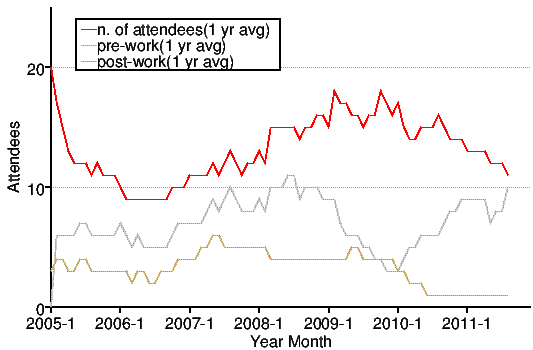
\includegraphics[width=0.7\hsize]{image201112/memberanalysis/attend.png}
\caption{$BEl5~%(%j%"(BDebian$BJY6/2q;vA02]Bj!&;v8e2]BjDs=P<B@S(B(12$B%v7n0\F0J?6Q(B)}\label{fig:attendandprepostwork}
\end{center}
\end{figure}

$BKh2s$N;22C<T$N?M?t$H!"$=$N:]$N%H%T%C%/$r8+$F$_$^$9!#(B
$B:#G/$b:rG/F1MM!"?M?tE*$K$OBg$-$/A}8:$O$"$j$^$;$s$,!"(B10$B7n$NC^GHBg$G$N3+:E$G$N;22C<T$,!":rG/$NC^GHBg$G$N$D$/$i$0$5$s$H$N9gF1JY6/2q$N;~$HF1$8;22C<T?t$G$7$?!#?7;2$N;22C<T$r4|BT$7$?C^GHBg@8$N;22C$O;W$C$?$[$I$G$O$J$+$C$?0lJ}!"=i;22C$J$N$K$o$6$o$6ET?4$+$iC^GHBg$^$G;22C$7$F$/$l$?J}$,0U30$HB?$+$C$?2s$G$7$?!#(B2009$BG/$+$i8+$k$H!"Bg3X$G$N3+:E$O$$$D$b$h$j;22C<T?t$*$h$S=i;22C<T$,A}$($k$N$G!"MhG/0J9_$bB3$1$F$$$/$HNI$$$G$7$g$&!#(B
$B$^$?!"%j%9%H$r$_$k$H!"Kh7n?tL>$O=i;22C<T$bKh7n$$$F!"$=$N$&$A0lIt$O(B2$B2sL\0J9_$b;22C$9$k?M$,$$$k$3$H$r9M$($k$H!"@h$[$I$N;22C?t$,2<9_798~$K$"$j$D$D!";vA02]Bj$NDs=P?t$,2#$P$$$G$"$k$N$O!"$A$c$s$H;vA02]Bj$rDs=P$9$k?M$,>oO"$K$J$k798~$K$"$k$N$G$O$J$$$+!"$H$b8+$l$^$9!#;vA02]Bj$NDs=PN($O0];}$7$D$D!";22C<T?t$OA}$d$7$F$$$/0Y$NBP:v$OI,MW$G$7$g$&!#(B


$B2q>l$r8+$k$H!":#G/$N2q>l$O!"$"$s$5$s$V$k2.7&0J30$N8xL14[$J$I$NMxMQ$,A}$($^$7$?!#(B
$B$^$?!":#G/$O#3G/A0$NApDE29@t!":rG/$NLZ99DE$KB3$-!";02sL\$N(BDebian$B29@t$r0KEl$N;34n29@t$G3+:E$7$^$7$?!#(B
Debian Hack Cafe$B$b(B6$B7n$4$m$+$i7n(B1$B2sDxEY$N%Z!<%9$G:F3+$7$F$$$k$h$&$G$9!#(B

\begin{table}[ht]
\begin{minipage}{0.5\hsize}
 \caption{$BEl5~%(%j%"(BDebian$BJY6/2q;22C?M?t(B(2005-2006$BG/(B)}\label{tab:count}
 \begin{center}
  \begin{tabular}{|l|c|p{10em}|}
 \hline
   & $B;22C?M?t(B & $BFbMF(B \\
 \hline
   2005$BG/(B1$B7n(B & 21 & $BHkL)(B\\
   2005$BG/(B2$B7n(B & 10 & debhelper 1\\
   2005$BG/(B3$B7n(B & 8 &  ($BAaD+(B) debhelper 2$B!"(Bsocial contract\\
   2005$BG/(B4$B7n(B & 6 & debhelper 3\\
   2005$BG/(B5$B7n(B & 8 & DFSG$B!"(Bdpkg-cross$B!"(Blintian/linda\\
   2005$BG/(B6$B7n(B & 12 & alternatives$B!"(Bd-i\\
   2005$BG/(B7$B7n(B & 12 & toolchain$B!"(Bdpatch\\
   2005$BG/(B8$B7n(B & 7 & Debconf$B;22CJs9p!"(BITP$B$+$i%"%C%W%m!<%I$^$G(B\\
   2005$BG/(B9$B7n(B & 14 & debconf\\
   2005$BG/(B10$B7n(B & 9 & apt-listbugs$B!"%P%0%l%]!<%H!"(Bdebconf$BK]Lu!"(Bdebbugs\\
   2005$BG/(B11$B7n(B & 8 & DWN$BK]Lu%U%m!<!"(Bstatoverride\\
   2005$BG/(B12$B7n(B & 8 & $BK:G/2q(B\\
   2006$BG/(B1$B7n(B & 8 & policy$B!"(BDebian$BJY6/2q$G$d$j$?$$$3$H(B\\
   2006$BG/(B2$B7n(B & 7 & policy$B!"(Bmultimedia \\
   2006$BG/(B3$B7n(B & 30 & OSC: debian$BJY6/2q!"(Bsid \\
   2006$BG/(B4$B7n(B & 15 & policy$B!"(B\LaTeX{} \\
   2006$BG/(B5$B7n(B & 6 & mexico \\
   2006$BG/(B6$B7n(B & 16 & debconf$B!"(Bcowdancer\\
   2006$BG/(B7$B7n(B & 40 & OSC-Do: MacBook Debian \\
   2006$BG/(B8$B7n(B & 17 & 13$B<9G0(B \\
   2006$BG/(B9$B7n(B & 12 & $BK]Lu!"(BDebian-specific$B!"(Boprofile \\
   2006$BG/(B10$B7n(B & 23 & network$B!"(Bi18n$B2q5D!"(BFlash$B!"(Bapt \\
   2006$BG/(B11$B7n(B & 20 & $B4X@>3+:E!'(B bug$B!"(Bsid$B!"(Bpackaging \\
   2006$BG/(B12$B7n(B & 14 & $BK:G/2q(B \\
 \hline
  \end{tabular}
 \end{center}
\end{minipage}
\begin{minipage}{0.5\hsize}
 \caption{$BEl5~%(%j%"(BDebian$BJY6/2q;22C?M?t(B(2007-2008$BG/(B)}\label{tab:count2007}
 \begin{center}
  \begin{tabular}{|l|c|p{10em}|}
 \hline
 & $B;22C?M?t(B & $BFbMF(B\\
 \hline
   2007$BG/(B1$B7n(B & 15 & $B0lG/$r4k2h$9$k(B \\
   2007$BG/(B2$B7n(B & 13 & dbs, dpatch\\
   2007$BG/(B3$B7n(B & 80 & OSC$B2>A[2=(B \\
   2007$BG/(B4$B7n(B & 19 & quilt, darcs, git\\
   2007$BG/(B5$B7n(B & 23 & etch, pbuilder, superh \\
   2007$BG/(B6$B7n(B & 4 & $B%(%8%s%P%i3+:E!'(BDebconf7 $B<B67Cf7Q(B \\
   2007$BG/(B7$B7n(B & 18 & Debconf7 $B;22CJs9p(B\\
   2007$BG/(B8$B7n(B & 25 & cdn.debian.or.jp \\
   2007$BG/(B9$B7n(B & 14 & exim \\
   2007$BG/(B10$B7n(B & 30 & OSC Tokyo/Fall(CUPS) \\
   2007$BG/(B11$B7n(B & 19 & live-helper, tomoyo linux kernel patch, server\\
   2007$BG/(B12$B7n(B & 11 & $BK:G/2q(B\\
   2008$BG/(B1$B7n(B & 23 & $B0lG/$r4k2h$9$k(B \\
   2008$BG/(B2/29,3/1 & 36 & OSC  \\
   2008$BG/(B3$B7n(B & 37 & $B%G!<%?$@$1$N%Q%C%1!<%8!"%i%$%;%s%9(B \\
   2008$BG/(B4$B7n(B & 17 & $B%P%$%J%j%Q%C%1!<%8(B \\
   2008$BG/(B5$B7n(B & 20 & $BJ#?t$N%P%$%J%j%Q%C%1!<%8(B \\
   2008$BG/(B6$B7n(B & 10 & debhelper \\
   2008$BG/(B7$B7n(B & 17 & Linux kernel patch / module $B%Q%C%1!<%8(B \\
   2008$BG/(B8$B7n(B & 10 & Debconf IRC$B2q5D$H(BDebian$B29@t(B \\
   2008$BG/(B9$B7n(B & 17 & po4a, $B!V(BDebian $B%a%s%F%J$N$*;E;v!W(B \\
   2008$BG/(B10$B7n(B & 11? & OSC Tokyo/Fall \\
   2008$BG/(B11$B7n(B & 17 & $B!V$=$N>l$GJY6/2q;qNA$r:n@.$7$A$c$(!W(B Debian $B$r;H$C$?(B \LaTeX{} $B869F:n@.9g=I(B \\
   2008$BG/(B12$B7n(B & 12 & $BK:G/2q(B \\
 \hline
  \end{tabular}
 \end{center}
\end{minipage}
\end{table}

\begin{table}[t]
\begin{minipage}{0.5\hsize}
 \caption{$BEl5~%(%j%"(BDebian$BJY6/2q;22C?M?t(B(2009-2010$BG/(B)}\label{tab:count2009}
 \begin{center}
  \begin{tabular}{|l|c|p{10em}|}
 \hline
 & $B;22C?M?t(B & $BFbMF(B\\
 \hline
   2009$BG/(B1$B7n(B & 12 & $B0lG/$r4k2h$9$k(B \\
   2009$BG/(B2$B7n(B & 30 & OSC $B%Q%C%1!<%8%O%s%:%*%s(B\\
   2009$BG/(B3$B7n(B & 23 & Common Lisp, $B%Q%C%1!<%8:n@.(B \\
   2009$BG/(B4$B7n(B & 15 & Java Policy, ocaml, $B3+H/%o!<%/%U%m!<(B\\
   2009$BG/(B5$B7n(B & 13 & MC-MPI$B%Q%C%1!<%82=!"(BErlang$B!"(BAndroid$B%"%W%j!"(BDDTP \\
   2009$BG/(B6$B7n(B & 14 & DDTP$B!&(BDDTSS$B!"(Bbsdstats$B%Q%C%1!<%8!"(BDebian kFreeBSD\\
   2009$BG/(B7$B7n(B & 4 & $B%9%Z%$%s$K$F(BDebconf 9\\
   2009$BG/(B8$B7n(B & 14 & $B%9%Z%$%s(B Debconf 9 $B;22CJs9p(B \\
   2009$BG/(B9$B7n(B & 26 & GPG$B%-!<%5%$%s%Q!<%F%#!<(B \\
   2009$BG/(B10$B7n(B & 30 & OSC Tokyo Fall\\
   2009$BG/(B11$B7n(B & 12 & Octave, R, gnuplot, auto-builder \\
   2009$BG/(B12$B7n(B & 10 & $BK:G/2q(B\\
   2010$BG/(B1$B7n(B & 17 &  $BEl5~Bg3X$K$F?7G/2q(B \\
   2010$BG/(B2$B7n(B & 11 & Debian$B29@t(B,ocaml,haskell \\
   2010$BG/(B3$B7n(B & 12 & weka,fftw,dpkg v3 quilt \\
   2010$BG/(B4$B7n(B & 15 & upstart,piuparts,debtags \\
   2010$BG/(B5$B7n(B & 22 & $BC^GHBg3X(B,kernel \\
   2010$BG/(B6$B7n(B & 12 & OSC-Do$B%j%O!<%5%k(B  \\
   2010$BG/(B7$B7n(B & 0 & $B%-%c%s%;%k(B  \\
   2010$BG/(B8$B7n(B & 3 & Debconf (NYC) \\
   2010$BG/(B9$B7n(B & 30 & OSC Tokyo/Fall \\
   2010$BG/(B10$B7n(B & 13 & $B26$N(BDebian$B$J0lF|(B \\
   2010$BG/(B11$B7n(B & 15 & ext4,btrfs,nilfs,ceph \\
   2010$BG/(B12$B7n(B & 14 &  cacert, libsane \\
 \hline
  \end{tabular}
 \end{center}
\end{minipage}
\begin{minipage}{0.5\hsize}
 \caption{$BEl5~%(%j%"(BDebian$BJY6/2q;22C?M?t(B(2011$BG/(B)}\label{tab:count2011}
 \begin{center}
  \begin{tabular}{|l|c|p{10em}|}
 \hline
 & $B;22C?M?t(B & $BFbMF(B\\
 \hline
   2011$BG/(B1$B7n(B & 12 & $B2.7&(B,Kinect,$B%"%s%1!<%H%7%9%F%`(B,CACert$B%5%$%s2q(B \\
   2011$BG/(B2$B7n(B & 13 & $BKL?7=I@8363X=,4[(B,HDFS,Debian Game Team \\
   2011$BG/(B3$B7n(B & ? & OSC Tokyo/Spring,CACert ATE Tokyo \\
   2011$BG/(B4$B7n(B & 12 & IIJ,backports,initramfs,$B7n4)(BPPC64 \\
   2011$BG/(B5$B7n(B & 15 & $B8M;3@8363X=,4[(B,Apache2$B%b%8%e!<%k(B,Debian on $B%K%U%/%i(B,Debian/m68k,$B7n4)(BPPC64 \\
   2011$BG/(B6$B7n(B & 17 & $BEl5~%*%j%s%T%C%/%;%s%?!<(B,$B%I%-%e%a%s%H=hM}7O(B,2011$B:F7W2h(B \\
   2011$BG/(B7$B7n(B & 3 & DebConf11 \\
   2011$BG/(B8$B7n(B & 12 & $B2.7&(B,$B%Q%C%1!<%8%s%04XO"(B, Debconf11$BJs9p(B \\
   2011$BG/(B9$B7n(B & 9 & $B;34nN94[(B,Debian$B29@t(B2011 \\
   2011$BG/(B10$B7n(B & 22 & $BC^GHBg3X(B,Haskell,LaTeX,$B%l%]!<%H<+F0@8@.(B,$B7n4)(Bdebhelper$B3+;O(B \\
   2011$BG/(B11$B7n(B & ? & OSC Tokyo/Fall \\
   2011$BG/(B12$B7n(B & 9 & $B%9%/%&%'%"!&%(%K%C%/%9(B,quilt$B$G(Bporting,$B7n4)(Bdebhelper,$B?6$jJV$j(B \\
 \hline
  \end{tabular}
 \end{center}
\end{minipage}
\end{table}

\clearpage

%-------------------------------------------------------------------------------
\dancersection{$B4X@>(BDebian$BJY6/2q(B 2011$BG/$N?6$jJV$j$H(B2012$BG/$N4k2h(B}{Debian JP}
%-------------------------------------------------------------------------------
\index{debianjp@Debian JP}
\index{$B$+$s$5$$(BDebian$B$Y$s$-$g$&$+$$(B@$B4X@>(BDebian$BJY6/2q(B}
\index{2011$B$M$s(B@2011$BG/(B}

$B=i2s$,(B2007$BG/(B3$B7n$J$N$G!"(B2011$BG/$G(B5$BG/L\$K$J$j$^$9$M!#(B

\subsection{$BJY6/2qA4BN(B}

$BKh2s$N%;%C%7%g%s$K$D$$$F$G$9$,!"(B
$B:#G/$O%Q%C%1!<%8:n@.$d(BBTS$B$K4X$9$kBj:`$,B?$/07$o$l$^$7$?!#(B
$BDjHV$N%M%?(B(Debian$B$NF~LgE*$J$*OC!"%i%$%;%s%9!"%Q%C%1!<%8:n@.!"(BBTS)$B$J$I$NBj:`$O(B
$BKhG/99?7$5$l$F$$$/$Y$-Bj:`$J$N$G(B, $B:#8e$b7+$jJV$707$C$F$$$-$?$$=j$G$9!#(B
$B;vA02]Bj$GDs=P$5$l$F$$$?!V%$%s%9%H!<%kBg2q!W$N$h$&$J=i?4<T9V=,$b$d$C$F$_$?$$(B
$B=j$G$9$M!#(B

$B$^$?!":rG/$+$i;vA02]Bj$NDs=P$,IaDL$K$J$C$F$-$^$7$?$N$G!"(B
$BMhG/$+$i$O;v8eE}7W(B($B%"%s%1!<%H(B)$B$bDs=P$7$F$b$i$*$&$+(B, $B$J$s$F9M$($F$$$^$9!#(B

$B1?1D$K4X$7$F$O!">oO"$5$s$@$C$?2OED$5$s$,1?1DB&$K$J$j!"(BDebian JP Project
$B$X2CF~$5$l$^$7$?!#$^$?!":#2s$NH/I=$K$"$kDL$jARI_$5$s$,(B DD $B$K$J$k$?$a(B
$B$N(B NM $B%W%m%;%9$X?=@A$5$l$F$$$^$9!#(B

$B%$%Y%s%H;22C$K$D$$$F$O!"(BOSC Kansai@ Kobe, OSC Hokkaido, OSC Kansai@
Kyoto, KOF $B$K;22C$7$^$7$?!#JY6/2q$+$i(B fork $B$7$?(B GPG $B%-!<%5%$%s%Q!<%F%#$b(B
$BKh2s<B;\$5$l$F$$$^$9!#:#8e$b7QB3$7$F;22C$9$kM=Dj$G$9!#(B

\subsection{$B3+:E<B@S(B}

$B4X@>(BDebian$BJY6/2q$N=P@J>u67$r3NG'$7$F$_$^$7$g$&!#%0%i%U$G8+$k(B
$B$H(B\fgref{fig:kansaipeoplechart}$B$K$J$j$^$9!#$^$?!"Kh2s$N;22C<T$N?M?t$H$=$N(B
$B:]$N%H%T%C%/$r(B \tbref{tab:count2011kansai} $B$K$^$H$a$^$7$?!#%0%i%UCf$N9u@~(B
$B$O;22C?M?t(B, $B@V@~$O(B1$BG/$N0\F0J?6Q$G$9!#;22C?M?t$,(B$0$$B$H$J$C$F$$$k$H$3$m$O?M(B
$B?t$,=87W$5$l$F$$$J$$(Bor$B3+:E$5$l$J$+$C$?7n$G$9$N$G!"7gB;CM=hM}$r$7$?J}$,NI$$$G$9$M(B%
\footnote{R$B;H$C$?;v$J$$$N$G:#F|$O4V$K9g$$$^$;$s$G$7$?(B}$B!#(B

Debian$BJY6/2q?=$79~$_%7%9%F%`$r;HMQ$9$k$h$&$K$J$j(B, $B;vA02]Bj$r@_Dj$9$k$3$H(B
$B$bB?$/$J$j$^$7$?!#$^$?(B, $B%"%s%1!<%H%7%9%F%`$b2TF0$9$k$h$&$K$J$k$G$7$g$&$+(B
$B$i!":#8e$O;vA02]Bj$H;v8e2]Bj$N%0%i%U$rDI2C$7$h$&$H;W$C$F$$$^$9!#(B


\begin{figure}[h]
  \begin{center}
    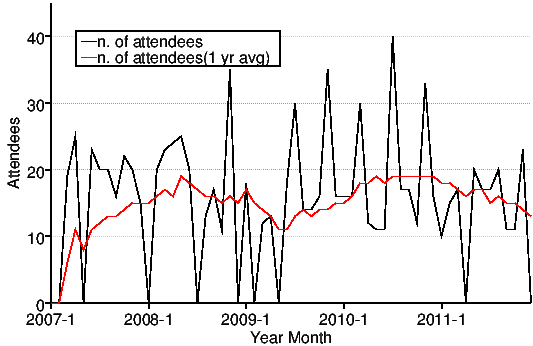
\includegraphics[width=.8\hsize]{image201112/memberanalysis/kansai.png}
  \end{center}
  \caption{$B4X@>$N;22C?M?t?d0\(B($B;22C?M?t$H(B12$B%v7n0\F0J?6Q(B)}
  \label{fig:kansaipeoplechart}
\end{figure}
\begin{table}
  \begin{minipage}{0.5\hsize}
    \caption{$B4X@>(BDebian$BJY6/2q$N;22C?M?t$H%H%T%C%/(B(2007$BG/(B)}
    \begin{center}
      \begin{tabular}{|l|c|p{10em}|}
        \hline
                   & $B;22C?M?t(B & $BFbMF(B \\
        \hline
        2007$BG/(B3$B7n(B  & 19       & $B3+:E$K$"$?$j(B \\
        2007$BG/(B4$B7n(B  & 25       & goodbye$B!"(Byoutube$B!"%W%m%8%'%/%H%H%i%C%+!<(B\\
        2007$BG/(B6$B7n(B  & 23       & $B<R2q7@Ls!"%F!<%^!"(Bdebian/rules$B!"(Bbugreport\\
        2007$BG/(B7$B7n(B  & 20$BA08e(B   & OSC-Kansai \\
        2007$BG/(B8$B7n(B  & 20       & Inkscape$B!"(Bpatch$B!"(Bdpatch\\
        2007$BG/(B9$B7n(B  & 16       & $B%i%$%V%i%j!"K]Lu!"(Bdebtorrent\\
        2007$BG/(B10$B7n(B & 22       & $BF|K\8lF~NO!"(BSPAM$B%U%#%k%?(B\\
        2007$BG/(B11$B7n(B & 20$BA08e(B   & KOF \\
        2007$BG/(B12$B7n(B & 15       & $BK:G/2q!"(BiPod touch\\
        \hline
      \end{tabular}
    \end{center}
  \end{minipage}
  \begin{minipage}{0.45\hsize}
    \begin{center}
    \caption{$B4X@>(BDebian$BJY6/2q;22C?M?t(B(2008$BG/(B)}\label{tab:count2008kansai}
    \vspace{-1em}
      \begin{tabular}{|l|c|p{10em}|}
        \hline
                   & $B;22C?M?t(B & $BFbMF(B \\
        \hline
        2008$BG/(B2$B7n(B  & 20       & PC Cluster, GIS, \TeX \\
        2008$BG/(B3$B7n(B  & 23       & bug report, developer corner, GPG \\
        2008$BG/(B4$B7n(B  & 24       & coLinux, Debian GNU/kFreeBSD, sid \\
        2008$BG/(B5$B7n(B  & 25       & ipv6, emacs, ustream.tv\\
        2008$BG/(B6$B7n(B  & 20       & pbuilder, hotplug, ssl\\
        2008$BG/(B8$B7n(B  & 13       & coLinux \\
        2008$BG/(B9$B7n(B  & 17       & debian mentors, ubiquity, DFSG\\
        2008$BG/(B10$B7n(B & 11       & cdbs,cdn.debian.or.jp \\
        2008$BG/(B11$B7n(B & 35       & KOF \\
        2008$BG/(B12$B7n(B & ?        & TeX$B;qNA:n@.%O%s%:%*%s(B\\
        \hline
      \end{tabular}
    \end{center}
  \end{minipage}
\end{table}
\begin{table}
  \begin{minipage}{0.5\hsize}
    \caption{$B4X@>(BDebian$BJY6/2q$N;22C?M?t$H%H%T%C%/(B(2009-2010)}
    \begin{center}
      \begin{tabular}{|l|c|p{10em}|}
        \hline
                   & $B;22C?M?t(B & $BFbMF(B \\
        \hline
        2009$BG/(B1$B7n(B  & 18       & DMCK, LT \\
        2009$BG/(B3$B7n(B  & 12       & Git \\
        2009$BG/(B4$B7n(B  & 13       & Installing sid, Mancoosi, keysign \\
        2009$BG/(B6$B7n(B  & 18       & Debian Live, bash\\
        2009$BG/(B7$B7n(B  & 30?      & OSC2009Kansai \\
        2009$BG/(B8$B7n(B  & 14       & DDTSS, lintian \\
        2009$BG/(B9$B7n(B  & 14       & reportbug, debian mentors\\
        2009$BG/(B10$B7n(B & 16       & gdb, packaging \\
        2009$BG/(B11$B7n(B & 35       & KOF2009 \\
        2009$BG/(B12$B7n(B & 16       & GPS program, OpenStreetMap \\
        2010$BG/(B1$B7n(B  & 16       & Xen, 2010$BG/4k2h(B \\
        2010$BG/(B2$B7n(B  & 16       & $B%l%s%?%k%5!<%P$G$NMxMQ(B, GAE \\
        2010$BG/(B3$B7n(B  & 30?      & OSC2010Kobe \\
        2010$BG/(B4$B7n(B  & 12       & $B%G%9%/%H%C%W4D6-(B, $B@55,I=8=(B \\
        2010$BG/(B5$B7n(B  & 11       & ubuntu, squeeze \\
        2010$BG/(B6$B7n(B  & 11       & debhelper7, cdbs, puppet \\
        2010$BG/(B7$B7n(B  & 40?      & OSC2010Kyoto \\
        2010$BG/(B8$B7n(B  & 17       & emdebian, kFreeBSD \\
        2010$BG/(B9$B7n(B  & 17       & $B%?%$%k(BWM \\
        2010$BG/(B10$B7n(B & 12       & initramfs, debian live \\
        2010$BG/(B11$B7n(B & 33       & KOF2010 \\
        2010$BG/(B12$B7n(B & 14       & Proxmox, annual review \\
        \hline
      \end{tabular}
    \end{center}
  \end{minipage}
  \begin{minipage}{.45\linewidth}
    \caption{$B4X@>(BDebian$BJY6/2q$N;22C?M?t$H%H%T%C%/(B(2011)}\label{tab:count2011kansai}
    \begin{center}
      \begin{tabular}{|l|c|p{10em}|}
        \hline
        $B3+:EG/7n(B  & $B;22C?M?t(B & $BFbMF(B \\
        \hline
        2011$BG/(B1$B7n(B &10        & BTS, Debian GNU/kFreeBSD\\
        2011$BG/(B2$B7n(B &15        & pbuilder, Squeeze$B%j%j!<%9%Q!<%F%#(B\\
        2011$BG/(B3$B7n(B &17        & $B%i%$%;%s%9(B, Debian$B$N%I%-%e%a%s%H4XO"(B\\
        2011$BG/(B4$B7n(B &25        & OSC 2011 Kansai @ Kobe, GPG $B%-!<%5%$%s%Q!<%F%#(B \\
        2011$BG/(B5$B7n(B &20        & vi, dpkg \\
        2011$BG/(B6$B7n(B &17        & IPv6, vcs-buildpackage{svn, git}\\
        2011$BG/(B7$B7n(B &17        & OSC 2011 Kansai @ Kyoto, GPG $B%-!<%5%$%s%Q!<%F%#(B\\
        2011$BG/(B8$B7n(B &20        & Debian$B%Q%C%1!<%8:n@.%O%s%:%*%s(B\\
        2011$BG/(B9$B7n(B &11        & vcs-buildpackage{bzr, git}\\
        2011$BG/(B10$B7n(B&11        & Emacs, vim $B$N3HD%$N(BDebian$B%Q%C%1!<%8(B, $BK]Lu(B\\
        2011$BG/(B11$B7n(B&23        & KOF 2011\\
        2011$BG/(B12$B7n(B&13        & NM$B%W%m%;%9(B, BTS\\
        \hline
      \end{tabular}
    \end{center}
  \end{minipage}
\end{table}


\clearpage

%-------------------------------------------------------------------------------
\dancersection{$BEl5~%(%j%"(BDebian$BJY6/2q$N3+:EJ}K!(B}{$BLnEg(B $B5.1Q(B}
%-------------------------------------------------------------------------------
\index{$B$H$&$-$g$&$($j$"$G$S$"$s$Y$s$-$g$&$+$$$N$+$$$5$$$[$&$[$&(B@$BEl5~%(%j%"(BDebian$BJY6/2q$N3+:EJ}K!(B}

\subsection{$B$O$8$a$K(B}

$BEl5~%(%j%"(BDebian$BJY6/2q$G$O!"KhG/(B12$B7n9f;qNA$G$OJY6/2q$N3+:EJ}K!$K$D$$$F$^(B
$B$H$a$F$$$^$9!#:#2s$OLnEg$,0lDL$j$NN.$l$r$^$H$a$^$9!#$3$l$rFI$a$P!"$"$J$?$b(B
$BEl5~%(%j%"(BDebian$BJY6/2q$r3+$1$k$O$:!*(B

\subsection{$BEl5~%(%j%"(BDebian$BJY6/2q$r3+$/;~$N%9%1%8%e!<%k(B}

% $BEl5~%(%j%"(BDebian$BJY6/2q$OI=(B\ref{tab:meeting-schedule}$B$N%9%1%8%e!<%k$G9T$$$^$9!#(B

\begin{table}[ht]
\begin{center}
\small
\begin{tabular}{|p{12em}|p{31em}|}
\hline
$B;~4|(B&$B:n6HFbMF(B \\
\hline\hline
$B3+:E(B2$B%v7nA0(B & $B>l=j$r3NJ]$7$^$9!#2q5D<<$O#2%v7nA0$KM=Ls$7$J$$$HKd$^$j$d$9$$$G$9!#(B\\
\hline
$B3+:E(B2$B%v7nA0$+$i(B1$B%v7nA0(B & $BJY6/2q$N%F!<%^$H!";vA02]Bj$r7h$a$^$9!#(B\\
\hline
$B3+:E(B1$B%v7nA0(B & $BJY6/2q$N%F!<%^$K1h$C$?869F$rJg=8$7$^$9!#;~4VOH$K$"$o$;$?H/I=$,Kd$^$i$J$$>l9g!"(B
$BH/I=<T$rOH$,Kd$^$k$^$G!"C5$9;v$K$J$j$^$9!#$^$?!"3+:E$K$"$?$j!":n6H$NJ,C4$,I,MW$J;~$O!"$3$N;~(B
$B$0$i$$$K3d$jEv$F$r40N;$7$^$9!#$^$?!"1c2q$N>l=j$K$D$$$F!"3NJ]$,:$Fq$J;v$,M=A[$5$l$k>l9g$O!"(B
$B$"$i$+$8$a@J$N$_M=Ls$7$F$*$-$^$9!#(B\\
\hline
$B3+:E(B2$B=54VA0$^$G$K(B & Debian$BJY6/2qM=Ls%7%9%F%`(B\url{http://debianmeeting.appspot.com}$B$KM=LsEPO?(B
$B%Z!<%8$r:n@.$7$^$9!#(BDebian JP Blog \url{http://www.debian.or.jp/}$B5Z$S!"(B
Debian$BJY6/2q(BWeb$B%5%$%H(B \url{http://tokyodebian.alioth.debian.org/} $B$KJY6/2q$NFbMF$rDs<($7$^$9!#(B
$B%a!<%k$G(B debian-users $B%a!<%j%s%0%j%9%H$K%"%J%&%s%9$rEj$2$^$9!#(B
Debian JP twitter $B$d(B mixi Debian $B%3%_%e%K%F%#!<$J$I$K$b%"%J%&%s%9$9$k$3$H$,B?$$$G$9!#(B\\
\hline
$B3+:E#1=54VA0(B & $BH/I=<T$OJY6/2q;qNAMQ%j%]%8%H%j$K;qNA$r%3%_%C%H$7$^$9!#(B\\
\hline
$B3+:E#2F|A0!!(B& $B;22C<T$NJg=8$NDy@Z$j$r9T$$$^$9!#$3$N;~$^$G$KB7$C$?;vA02]Bj$rJY6/2q;qNA$K%^!<%8$7$^$9!#(B\\
\hline
$B3+:E(B1$BF|A0!!(B& kinkos$BEy$N0u:~@=K\%5!<%S%9$K869F0u:~$*$h$S@=K\$r0MMj$7$^$9!#(B\\
\hline
$B3+:EEvF|!!(B& \begin{enumerate}
  \item $B;22C<T$+$iHqMQ$N2s<}$H=87W$r$7$^$9!#(B
  \item $BJY6/2q$rDj9o$I$*$j$K3+:E$7$^$9!#(B
  \item $B;J2q<T!"H/I=<T$H6(NO$7$F;~4VFb$KJY6/2q$r=*N;$7$^$9!#(B
  \item $B1c2q$N>l=j$N3NJ]$,:$Fq$G$J$$;~$O!"1c2q$N>l=j$rM^$($^$9!#(B
  \item $B1c2q$N3+:E!"1c2q$N2q7W$r$7$^$9!#(B
\end{enumerate} \\
\hline
$B3+:E8e!!(B& Debian$BJY6/2qM=Ls%7%9%F%`$+$i%"%s%1!<%H$r$*$/$j$^$9!#(B \\
\hline
12$B7n!!(B& $BJY6/2q$N%"%s%1!<%H7k2L$J$I$r0lG/J,=87W$7$FH/I=$7$^$9!#(B \\
\hline
\end{tabular}
\caption{$BA4BN%9%1%8%e!<%k(B}
\label{tab:meeting-schedule}
\end{center}
\end{table}

\subsection{$BEl5~%(%j%"(BDebian$BJY6/2q$N3+:ED4@0(B}

$BEl5~%(%j%"(BDebian$BJY6/2q$N3+:ED4@0$O@lMQ$N%a!<%j%s%0%j%9%H$,$"$j!"IaCJ$O$3$A$i$GD4@0$,9T$o$l$^$9!#(B
$B1?1D<T@lMQ$N%a!<%j%s%0%j%9%H$G!"0lIt$N%3%"%a%s%P!<$N$_$,;22C$7$F$$$^$9!#(B
$B1?1D$K@Q6KE*$K;22C$7$?$$?M$OJY6/2q1?1D<T$KO"Mm$r<h$kI,MW$,$"$j$^$9!#(B

\subsection{$B=i$a$FEl5~%(%j%"(BDebian$BJY6/2q$N3+:E$rC4Ev$9$k>l9g$N;vA0=`Hw(B}

$B=i$a$FEl5~%(%j%"(BDebian$BJY6/2q$N3+:E$rC4Ev$9$k>l9g0J2<$N9`L\$,=`Hw$7$F$"$k$H(B
$B%9%`!<%:$G$9!#(B

\begin{enumerate}
\item Debian JP Project$B$NDs6!$9$k%5!<%P!<$X%m%0%$%s$G$-$k%"%+%&%s%H(B\\
Debian JP Blog$B$r99?7$9$k:]$KI,MW$K$J$j$^$9!#(B
$B$3$l$ODL>o(BDebian JP Project$B$N2q0w$K$J$k$H$-$KIUM?$5$l$^$9!#(B
$B2q0w$G$J$$?M$O2q0w$K%3%_%C%H$7$F$b$i$&$h$&0MMj$9$kI,MW$,$"$j$^$9!#(B

\item \url{http://alioth.debian.org/}$B%"%+%&%s%H(B
$B;qNA$NJT=8Ey$r9T$&:]$KI,MW$K$J$j$^$9!#(B
$B%"%+%&%s%H$r<hF@$7$?$i!"%a!<%j%s%0%j%9%H$G(Btokyodebian$B%0%k!<%W8"8B$K=jB0$5$;$F$[$7$$;]!"(B
$B<hF@$7$?%"%+%&%s%HL>$r1h$($F0MMj$7$^$9!#$3$N%"%+%&%s%H$OC/$G$b<hF@2DG=$G$9!#(B

\end{enumerate}

$B$^$?!"JY6/2q$N44;vC4Ev$N>l9g$KI,MW$JCN<1$H%3%s%T%e!<%?$N4D6-$O0J2<$K$J$j$^$9!#(B

\begin{enumerate}
\item Debian$B$,F0:n$7!"%$%s%?!<%M%C%H$,MxMQ$G$-$k(BPC$B$NMQ0U(B
\item ssh,emacs,muse-el,git$B!"(Bsubversion$B$N4pK\A`:n$K$D$$$F$NCN<1(B
\item $B%V%i%&%6$H(BHTML$B$N5-:\$NCN<1(B
\item \url{http://alioth.debian.org/},\url{http://qwik.jp/}$B$N;H$$J}$NCN<1(B
\item \LaTeX{}$B$NCN<1(B
\end{enumerate}

$B$o$+$i$J$$$3$H$d:$$C$?$3$H$,$"$l$P%a!<%k$d%a!<%j%s%0%j%9%H$GJ9$$$F$_$^$7$g$&!#(B

\subsection{$BEl5~%(%j%"(BDebian$BJY6/2q$N7G<($N=P$7J}(B}

\url{http://www.debian.or.jp/}$B$K7G<($r=P$9>l9g$NJT=8$N;EJ}$O!"(B
\url{http://www.debian.or.jp/project/webmasters.html}$B$K$=$N5-:\$,$"$j$^$9!#(B
$B<B:]$K$O!"(Bsubversion$B$G%j%]%8%H%j$r$H$C$F$-$F!"(B\\
\texttt{./www.debian.or.jp/blosxom/ data/events/tokyodebian-XX.d} (XX$B$OBh(BXX$B2s$r<($7$^$9!K$r(B
$B:n@.$7$^$9!#(B

\url{http://debianmeeting.appspot.com/eventadmin/edit?eventid=}$B$N%U%)!<%`$NJT=8(B
$B$O%U%)!<%`$K1h$C$F>pJs$rF~$l$k$@$1$G$9!#$?$@!":Y$+$$;v$O!"(B\url{http://tokyodebian.alioth.debian.org/YYYY-MM.html}$B$X$N%j%s%/$r(BURL$B$N(B
$BMs$K;XDj$7!"$=$A$i$r;2>H$7$F$b$i$$$^$9!#(B

\url{http://tokyodebian.alioth.debian.org/}$B$X$O!"(B\url{http://qwik.jp/$B%a!<%j%s%0%j%9%HL>(B}$B$N%H%C%W(B
$B%Z!<%8$K5-:\$5$l$F$$$k$d$jJ}$K=>$$$^$9!#<B:]$K$O(Bgit
$B$G(B\url{git+ssh://git.debian.org/git/tokyodebian/muse.git} $B%j%]%8%H%j$r(Bclone$B$7$F!"(Bmuse$B7A<0$GJT=8$7!"(Bmake publish$B$9$k;v$H$J$j$^$9!#(B

\clearpage

%-------------------------------------------------------------------------------
\dancersection{Debian$BJY6/2qM=Ls%7%9%F%`:FK,(B}{$B>e@n(B $B=c0l(B}
%-------------------------------------------------------------------------------
\index{Debian$B$Y$s$-$g$&$+$$$h$d$/$7$9$F$`(B@Debian$BJY6/2qM=Ls%7%9%F%`(B}
\index{python appengine}
\index{django}

Debian $BJY6/2qM=Ls%7%9%F%`$N3+H/3+;O$+$i(B2$BG/7P$A$^$7$?!#Ev=i$O1c2q7/$r%j%W%l!<(B
$B%9$9$k$?$a$KFM4S$G$D$/$j$"$2$?$b$N$G$9$,$[$\$=$N$^$^$N>uBV$G1?1D$5$l$F$$(B
$B$^$9!#LLE]$/$5$,$C$FE,Ev$K<BAu$7$?ItJ,!"%&%'%V%"%W%j%1!<%7%g%s$G5$$r$D$1(B
$B$k$Y$-$H$3$m$r$h$/$o$+$i$:$K=q$$$F$$$?ItJ,$,$"$C$?$N$G$$$^$+$i?6$jJV$C$F(B
$B$I$&$$$&2]Bj$,$"$C$?$N$+$r8!F$$7$^$9!#(B

\subsection{$B@H<e@-(B}

\subsubsection{POST/GET $B$N;H$$J,$1(B}

$BEv=i$a$s$I$/$5$+$C$?$N$G(Bpost$B$H(Bget$B$N%O%s%I%i$r0l=o$K$7$F$^$7$?!#$h$C$F!"(B
$B$"$i$f$k%Z!<%8$,(BGET$B$H(BPOST$B$NN>J}$GF0$/$h$&$K$J$C$F$$$^$9!#$=$l$rE,@Z$K(BGET
$B$H(BPOST$B$K$o$1$k$h$&$K$7$^$7$?!#(B

GET$B$O>pJs$N<hF@$N$_!"(BPOST$B$OEPO?$J$I$NI{:nMQ$N$"$k=hM}$KMxMQ$7$^$9!#(B

\index{XMLHttpRequest}
$B%V%i%&%6$N%;%-%e%j%F%#%b%G%k$H$7$F!"(Bsame-origin$B$8$c$J$$$H(BPOST$B$,$d$j$K$/(B
$B$$$h$&$K$J$C$F$$$^$9!#(BGET$B$O$?$H$($P(Bscript$B%?%0$d(Bimg$B%?%0$J$I$rKd$a9~$s$G$*(B
$B$1$P$$$/$i$G$bH/9T$G$-$^$9$,!"(BPOST$B$O(BXMLHttpRequest$B$NH/9T$,I,MW$G!"(B
XMLHttpRequest$B$K$O(Bsame-origin policy$B$,$"$j$^$9!#(B

$B0JA0$OG$0U$N%Z!<%8$+$i(Bscript$B%?%0$NKd$a9~$_$r$7$F>!<j$K(BDebian$BJY6/2q$KEPO?(B
$B$9$k$3$H$,2DG=$G$7$?$,!":#$O$=$l$,$G$-$J$$$h$&$K$J$C$F$$$^$9!#(B
$B$3$l$O>!<j$KM=Ls$9$k(BHTML$B%Z!<%8$NNc$G$9(B:
\begin{commandline}
<html>
  <head>
    <title>auto reserve exploit</title>
    <script
 src="http://localhost:8080/eventregister?eventid=df24a1e1de11c067c461537dce6394e0e51df6ad
&user_prework=&user_attend=attend&user_enkai_attend=enkai_attend&user_realname=myname">
    </script>
  </head>

  <body>
    <h1>auto reserve exploit</h1>
    <p>
      $B$\$/$O$^$A$A$c$s(B
    </p>
\end{commandline}

\subsubsection{HTML escaping}

$BEv;~$h$/$o$+$i$J$+$C$?$N$H$a$s$I$/$5$+$C$?$N$GF~NOJ8;zNs$N%5%K%?%$%:$H$+%(%9%1!<%W$H$+$^$C$?$/$7$F$^$;$s$G$7$?!#4X@>(BDebian$BJY6/2q$G$O(BHTML$B%?%0$rJY6/2q$NM=Ls%Z!<%8$N0FFbJ8$KF~NO$7$F(B
$B$$$?$h$&$G!"$=$l$G$3$N@H<e@-$,$=$b$=$bB8:_$9$k$N$K;W$$;j$j$^$7$?!#(B

$BG$0U$NJ8;zNs$r(BHTML$B$H$7$F=PNO$G$-$k$H!"G$0U$N(Bjavascript$B$N%3!<%I$r<B9T$9$k(B
$B$3$H$,$G$-$^$9!#$?$H$($P!"@bL@%Z!<%8$r3+$$$?=V4V$KM=LsEPO?$9$k%$%Y%s%H$r:n@.$9$k$3$H$,$G$-$^$9!#(B

\begin{commandline}
<script>
var xhr = new XMLHttpRequest();
xhr.open('POST', 'http://localhost:8080/eventregister');
xhr.withCredentials = true
xhr.setRequestHeader('Content-Type', 'application/x-www-form-urlencoded');
xhr.send('eventid=df24a1e1de11c067c461537dce6394e0e51df6ad&'
+ 'user_prework=%E3%81%BC%E3%81%8F%E3%81%AF%E3%81%BE%E3%81%A1%E3%81%A1%E3%82%83%E3%82%93&'
+ 'user_attend=attend&user_enkai_attend=enkai_attend&user_realname=hamachi');
</script>
\end{commandline}

\begin{wrapfigure}{r}{0.5\hsize}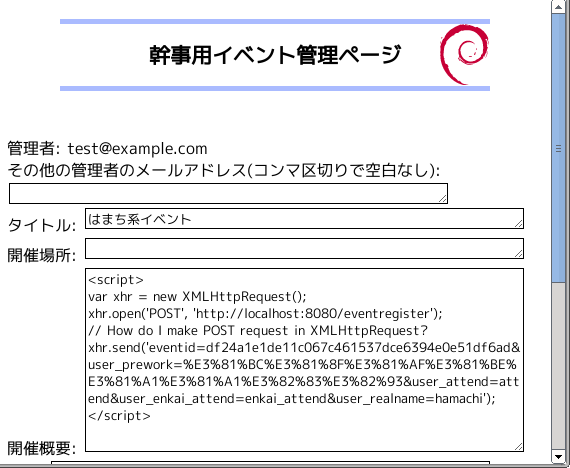
\includegraphics[width=\hsize]{image201201/xhr.png}\end{wrapfigure}

$B$7$+$?$,$J$$$N$GJ8;zNs$r%(%9%1!<%W$9$k$h$&$K$7$^$7$?!#(B
$BI{:nMQ$H$7$F(BHTML$B%?%0$r@bL@J8$KBG$A9~$`$3$H$,$G$-$J$$$h$&$K$J$C$F$$$^$9!#(B

\subsubsection{$BG$0U$N(BURL$BI=<((B}

Debian$BJY6/2qM=Ls%7%9%F%`$G$O@bL@J8$NI=<($,IO<e$JBe$o$j$KG$0U$N(BURL$B$r(B
iframe$B$GKd$a9~$_I=<($G$-$k$h$&$K$7$F$$$^$9!#DL>o4IM}$7$F$$$kJY6/2q$N(BWiki
$B%Z!<%8$rKd$a9~$`$3$H$GFs=E$K>pJs$r4IM}$7$J$/$F$9$`$h$&$K$H$$$&0U?^$G$9!#(B

URL$B$NCf$K$OFC<l$J$b$N$b$"$j$^$9!#(B\url{javascript:}$B$G;O$^$k(BURL$B$@$H$=$N(B
Javascript$B$N%3!<%I$r<B9T$9$k$3$H$,$G$-$^$9!#$G$-$F$bIaDL$NLr$K$ON)$?$J$5(B
$B$=$&$J$N$G(B\url{http://}$B0J30$O5v2D$7$J$$$h$&$K$7$F$*$-$^$7$?!#(B

$B$^$?!"(Biframe buster $B$H8F$P$l$k<jK!$K$h$j(Biframe
$B$+$iC&=P$G$-$k$h$&$G!"$=$&$$$&%Z!<%8$r(Biframe$B$NCf$G$R$i$$$F$$$k$D$b$j$K$J(B
$B$k$H%f!<%6$,8m2r$9$k2DG=@-$,$"$j$^$9!#(B

\index{iframe sandbox}
$B$9$Y$F$N%V%i%&%6$G%5%]!<%H$5$l$F$$$k$o$1$G$O$J$$$N$G$9$,!"(Biframe$B$K(B
sandbox$BB0@-$r$D$1$F$*$-(Bjavascript$B$J$I$N<B9T$r@)Ls$7$F$*$-$^$7$?!#(B

\subsection{$B2DG=@-$H@H<e@-$N%P%i%s%9(B}

$B:#2s$$$m$$$m$H@H<e@-$,$"$C$?$N$G$U$5$$$G$_$^$7$?!#$7$+$7!"@H<e@-$r:I$0$N(B
$B$b!"$"$j$&$kHo32$H$N%P%i%s%9$G9M$($k$Y$-$@$H;W$$$^$9!#(BDebian$BJY6/2q$KDs=P(B
$B$9$k;vA02]Bj$,O31L$9$k!">!<j$K1c2q$K;22C$9$k$3$H$K$J$C$F$$$kEy$NDxEY$N@H(B
$B<e@-$H!"<+M3$K(BHTML$B$,5-=R$G$-$k<+M3$H$I$A$i$,=EMW$+$H9M$($F$_$F$/$@$5$$!#(B
$B$9$3$7G:$^$7$$$H;W$$$^$;$s$+(B?

\clearpage

%-------------------------------------------------------------------------------
\dancersection{quilt$B$G(Bporting$B$7$F$_$?(B}{$B?yK\E5=<(B}
%-------------------------------------------------------------------------------
\index{quilt$B$G$]!<$F$#$s$0$7$F$_$?(B@quilt$B$G(Bporting$B$7$F$_$?(B}
\index{porting}
\index{kFreeBSD}

\subsection{$B$O$8$a$K(B}

debian$B$N%Q%C%1!<%8:n@.$G;HMQ$7$F$$$k%Q%C%A4IM}%D!<%k(Bquilt$B$K$D$$$F@bL@$7$^$9!#(B
$B$^$?(Bquilt$B$rMQ$$$F(BkFreeBSD$B$N(Bporting$B%Q%C%A$r:n@.$7$^$7$?$N$G!"$3$l$K$D$$$F$b@bL@$7$^$9!#(B

\subsection{Debian$B%Q%C%1!<%8$N%U%)!<%^%C%H(B}

$B8=:_(BDebian$B$G;HMQ$7$F$$$k<g$J%=!<%9%Q%C%1!<%8%U%)!<%^%C%H$O#2$D$G$9!#(B
\footnote{$BEl5~%(%j%"(BDebian$BJY6/2q(B 2010$BG/(B03$B7n9f!V(Bdpkg $B%=!<%97A<0(B "3.0(quilt)"$B!W(B $B5HLnM?;V?N(B}
\footnote{\url{http://wiki.debian.org/Projects/DebSrc3.0}}

\begin{itemize}
 \item{3.0(native)$B!'(Btarball$B#1$D$G9=@.$5$l$?%=!<%9%Q%C%1!<%8%U%)!<%^%C%H(B}
  \begin{itemize}
   \item{packagename-version.tar.ext}
   \item{packagename-version.dsc}
  \end{itemize}
  \item{3.0(quilt)$B!'$"$k%"%C%W%9%H%j!<%`$N(Btarball$B$H(BDebian$B%Q%C%1!<%8:n@.$K(B
$BI,MW$J(Btarball$B$KJ,3d$7$F$$$k%=!<%9%Q%C%1!<%8%U%)!<%^%C%H(B}
  \begin{itemize}
   \item{packagename-upstreamversion.orig.tar.ext}
   \item{packagename-upstreamversion.orig-component.tar.ext$B!JG$0U!K(B}
   \item{packagename-debianversion.debian.tar.ext}
   \item{packagename-debianversion.dsc}
  \end{itemize}
\end{itemize}

$B%=!<%9%Q%C%1!<%8%U%)!<%^%C%H$N>\:Y$O(B `dpkg-source(1)' $B%3%^%s%I$G3NG'$9$k$3$H$,$G$-$^$9!#(B
\footnote{man$B$K$h$k$H(B3.0(custom)$B!"(B3.0(git)$B!"(B3.0(bzr)$B$H$$$&%Q%C%1!<%87A<0$NDj5A$,$"$k$h$&$G$9!#(B}

$B%"%C%W%9%H%j!<%`$N%=!<%9%3!<%I$rL5=$@5$N$^$^(BDebian$B%Q%C%1!<%8$r:n@.$7$?>l9g!"(B
lintian$B=hM}$G%(%i!<$K$J$C$?$j!"(BDebian$B$N3+H/%]%j%7!<$rK~$?$;$J$$>l9g$,(B
$B$"$j$^$9!J%"%C%W%9%H%j!<%`$N%=!<%9%3!<%I$O(BIPv6$B$GF0:n$7$J$$!"$J$I!K!#(B
$B$=$N$H$-$O!"(B3.0(quilt)$B$N%=!<%9%Q%C%1!<%8%U%)!<%^%C%H$G%Q%C%1!<%8$r:n@.$7!"(B
$BI,MW$J%Q%C%A$rEv$F$F$+$i%=%U%H%&%'%"$N%S%k%I=hM}$r9T$&$3$H$GBP1~$5$;$^$9!#(B

\subsection{quilt$B%Q%C%1!<%8(B}
quilt$B$O(Bdebian$B%Q%C%1!<%8$r:n@.$9$k$H$-$K%Q%C%A%U%!%$%k$r4IM}$9$k%D!<%k$H$7$F(B
$B:NMQ$7$F$$$k%=%U%H%&%'%"$G$9!#(B
Debian$B%Q%C%1!<%8$H$7$FDs6!$7$F$*$j!"(Bapt$B$G%$%s%9%H!<%k$G$-$^$9!#(B

\begin{commandline}
# apt-get update
# apt-get install quilt
\end{commandline}

quilt$B%3%^%s%I$OJ#?t$N(Bpatch$B%U%!%$%k$r%9%?%C%/$K@Q$s$@$h$&$J%$%a!<%8$G!"(B
$B%Q%C%A$NE,MQ=gHV$r4IM}$7$^$9!#(B
\footnote{$BEl5~%(%j%"(BDebian$BJY6/2q(B 2007$BG/(B01$B7n9f!V%Q%C%A4IM}%D!<%k(Bquilt$B$N;H$$J}!W>.NS576)(B}
quilt$B%3%^%s%I$r;H$&$3$H$G!"%Q%C%1!<%8:n@.$KI,MW$J%Q%C%A$,J#?t$"$k>l9g$b(B
$B@5$7$/E,MQ$G$-!"ITMW$J%Q%C%A$,=P$F$-$?$H$-$K$=$N%Q%C%A$r<h$j=|$/$3$H$,MF0W$K(B
$B$J$j$^$9!#(B


\subsection{quilt$B$N;HMQNc!'(BDebian GNU/kFreeBSD$B8~$1$N(Bporting$B%Q%C%A:n@.(B}

\subsubsection{Debian GNU/kFreeBSD$B$H$O(B}
Debian Project$B$G3+H/$7$F$$$k(BOS$B$O(BLinux$B%+!<%M%k$rMQ$$$?!V(BDebian GNU/Linux$B!W$,M-L>$G$9$,!"(B
Linux$B%+!<%M%k0J30$rMQ$$$?(BDebian$B$,$"$j$^$9!#$=$N#1$D$H$7$F(BFreeBSD$B%+!<%M%k$rMQ$$$?!V(BDebian GNU/kFreeBSD$B!W(B
\footnote{\url{http://wiki.debian.org/Debian\_GNU/kFreeBSD}}$B$,$"$j!"%f!<%6%i%s%I$O(BDebian$B$J$N$G(B APT $B$,;H$(!"(B
$B%G%P%$%9$d%7%9%F%`%3!<%k$H$$$C$?%+!<%M%kFCM-$N5!G=$O(BFreeBSD$B%+!<%M%k$K=`$8$k!"$H$$$&FCD'$,$"$j$^$9!#(B
Debuan GNU/kFreeBSD$B$O0BDjHG$N%j%j!<%9$K$O;j$C$F$$$^$;$s$,!"F|!93+H/$,B3$1$i$l$F$$$^$9!#(B
$BK\9F$G$O0J9_!V(BDebian GNU/kFreeBSD$B!W$r!V(Bkfreebsd$B!W$HN,5-$7$^$9!#(B

\subsubsection{kfreebsd$B$N(Bporting$B:nK!(B}
Debian$B$N(Bporting$B4XO">pJs$*$h$S(Bkfreebsd$B$N(Bporting$B>pJs$O0J2<$K$"$j$^$9!#(B

\begin{itemize}
 \item{\url{http://www.debian.org/ports/}}
 \item{\url{http://www.debian.org/ports/kfreebsd-gnu/}}
 \item{\url{http://glibc-bsd.alioth.debian.org/porting/}}
\end{itemize}

$B!V(B\url{http://glibc-bsd.alioth.debian.org/porting/PORTING}$B!W$rFI$`$H(B
kfreebsd$B8~$1$K(Bporting$B$9$k$K$O0J2<$N3NG'$*$h$S=$@5$,9T$&$h$&$K$H$"$j$^$9!#(B

\begin{itemize}
 \item{Add our system name to checks here and there}
  \begin{itemize}
   \item{Makefile$B$d%9%/%j%W%HCf$N(Buname$B$J$I$r%A%'%C%/$7$F$/$@$5$$!#(B }
  \end{itemize}
 \item{debian/control files}
  \begin{itemize}
   \item{debian/control$B%U%!%$%k$G(BArchitecture$B$r(Blinux$B@lMQ%=%U%H%&%'%"$N>l9g$O!V(Blinux-any$B!WEy!"(B
CPU$B$N0c$$$N$_$G(BLinux$B!"(Bkfreebsd$B$O4X78$J$/;HMQ$G$-$k%=%U%H%&%'%"$N>l9g$O!V(Bany-i386$B!WEy$KJQ99$7$F$/$@$5$$!#(B}
  \end{itemize}
 \item{Libraries, your beloved enemy}
  \begin{itemize}
   \item{libtool$B!"(Baclocal.m4$B<~$j$KBP1~$7$F$/$@$5$$!#(B}
  \end{itemize}
 \item{Preprocessor Variables}
  \begin{itemize}
   \item{kfreebsd$B$N%7%9%F%`%^%/%m$O!V(B\_\_FreeBSD\_kernel\_\_$B!W!"(B
$B%P!<%8%g%s%^%/%m$O!V(B\_\_FreeBSD\_kernel\_version$B!W$J$N$GBP1~$7$F$/$@$5$$!#(B}
  \end{itemize}
 \item{Writing to devfs (kFreeBSD)}
  \begin{itemize}
   \item{FreeBSD$B%+!<%M%k$G$O!J(Budev$B$G$O$J$/!K(Bdevfs$B$r;H$&$h$&$K$7$F$/$@$5$$!#(B}
  \end{itemize}
 \item{RT signals}
  \begin{itemize}
   \item{FreeBSD$B%+!<%M%k$O!V(BPOSIX RT (realtime) signals$B!W$,$J$$$N$GJQ99$7$F$/$@$5$$!#(B}
  \end{itemize}
 \item{Get libc soname (6 or 6.1 on linux-gnu, 0.1 on kfreebsd-gnu, etc)}
  \begin{itemize}
   \item{$B;HMQ$9$k(Blibc$B$NL>A0$r%O!<%I%3!<%I$7$F$$$k%W%m%0%i%`$,$"$l$P=$@5$7$F$/$@$5$$!#(B}
  \end{itemize}
\end{itemize}


\subsubsection{kfreebsd$B$KBP1~$5$;$?$$%Q%C%1!<%8$H$=$N860x(B}

$B:#2s(Bporting$B$9$k%Q%C%1!<%8$O4{$K(Bkfreebsd$BMQ%Q%C%1!<%8$H$7$FB8:_$7$F$$$k(B
icewm$B$H$J$j$^$9!#(B
icewm$B$O%&%#%s%I%&%^%M!<%8%c$N%=%U%H%&%'%"$G7Z2w$JF0:n$r$9$k$N$,FCD'$G$9!#(B
icewm$B$G$O%?%9%/%P!<$K%P%C%F%j!<;DNL%"%$%3%s$rI=<($9$k5!G=$,$"$j$^$9$,(B
kfreebsd$B$G$OI=<($5$l$^$;$s!#(Blinux-i386$B5Z$S(Blinux-amd64$B$G$OI=<($5$l$k$?$a(B
kfreebsd$B$N(Bporting$B$,IT40A4$N2DG=@-$,$"$j$^$9!#(B

$B$^$:$O%S%k%I=`Hw$H%=!<%9%3!<%I$N%@%&%s%m!<%I$r9T$$$^$9!#(B

\begin{commandline}
# apt-get update
# apt-get build-dep icewm
$ apt-get source icewm
\end{commandline}
%$

$B%=!<%9%3!<%I$r!V(B\_\_FreeBSD\_\_$B!W5Z$S!V(B\_\_linux\_\_$B!W(Bgrep$B$9$k$H!"EE8;<~$j$N=hM}$G0J2<$N%^%/%m$,8!=P$5$l$^$9!#(B
\begin{commandline}
$ cd icewm-1.3.7/src
$ grep -nr __FreeBSD__ *
aapm.cc:30:#ifdef __FreeBSD__
aapm.cc:74:#if defined(__FreeBSD__) && defined(i386)
aapm.cc:99:#if defined(__FreeBSD__) && defined(i386)
aapm.cc:273:#ifndef __FreeBSD__
aapm.cc:333:#ifndef __FreeBSD__
aapm.cc:418:#ifndef __FreeBSD__
aapm.cc:463:#ifdef __FreeBSD__
aapm.cc:885:#ifndef __FreeBSD__
aapm.h:2:#if defined(linux) || (defined (__FreeBSD__)) || (defined(__NetBSD__) && defined(i386))
$B!J0J2<N,!K(B
$ grep -nr __linux__ *
($B$J$K$b$J$7(B)
\end{commandline}
%$

\_\_FreeBSD\_\_$B%^%/%m$O(BFreeBSD OS$B$r<($9%^%/%m$G$9$,!"(Bkfreebsd$B$G$O!V(B\_\_FreeBSD\_kernel\_\_$B!W$,%7%9%F%`!J87L)$K$O%+!<%M%k!K$r<($9%^%/%m$G$9!#$=$N$?$a%^%/%m$G%7%9%F%`$r@Z$jJ,$1$F$$$k$O$:$,(Bkfreebsd$B8~$1$N%Q%C%1!<%8%S%k%I;~$K(BLinux$B%+!<%M%k8~$1$N=hM}$,M-8z$J%3!<%I$H$7$F%S%k%I$5$l$F$7$^$$%P%C%F%j!<;DNL%"%$%3%s$NI=<($,$&$^$/F0:n$7$F$$$J$$$h$&$G$9!#(B

$B$=$N$?$a!":#2s$O$3$N%^%/%m$r!V(BPORTING$B!W$N5-=R$K=>$C$F0J2<$N$h$&$J=$@5$r9T$$$^$9!#(B

\begin{commandline}
$B!J=$@5A0!K(B#ifdef __FreeBSD__

$B!J=$@58e!K(B#if defined(__FreeBSD__) || defined(__FreeBSD_kernel__)
\end{commandline}
$B$3$l$G=$@5J}?K$,Dj$^$j$^$7$?$N$G!"(Bdebian$B%Q%C%1!<%8:n@.$K8~$1$F%Q%C%A$r:n@.$7$F$$$-$^$9!#(B

\subsection{quilt$B$NEP>l(B}
$B:#2s$O?75,$N%Q%C%A%U%!%$%k$H$J$k$?$a!"(Bquilt$B$N%Q%C%A%9%?%C%/$K?75,DI2C$7$^$9!#(B
$B$^$:!"(Bdebian/patches/series $B5-=R$5$l$F$*$k%Q%C%A%9%?%C%/$r8+$F$_$^$9!#(B

\begin{commandline}
$ tail -4 debian/patches/series
tray_hotfixes
imap_unseen
ifstate_exact_check
debian-changes-1.3.7~pre2-1.1
\end{commandline}
%$

$B<!$K(B\texttt{quilt new} $B$r<B9T$7!"8=:_$NJQ99FbMF$r(B kfreebsd\_porting\_aapm
$B$H$$$&%U%!%$%kL>$GJ]B8$7!"%9%?%C%/$KDI2C$7$^$9!#(B

\begin{commandline}
$ quilt new kfreebsd_porting_aapm
Patch kfreebsd_porting_aapm is now on top
\end{commandline}

$B<B9T2<8e$N%Q%C%A%9%?%C%/$O0J2<$N$h$&$K$J$j$^$9!#(B

\begin{commandline}
$ tail -4 debian/patches/series
imap_unseen
ifstate_exact_check
debian-changes-1.3.7~pre2-1.1
kfreebsd_porting_aapm
\end{commandline}
%$

$B$3$l$G%Q%C%A$rDI2C$G$-$k=`Hw$,$G$-$^$7$?!#(B
$B<!$K(Bporting$B$9$k$?$a$K=$@5$r9T$&%=!<%9%U%!%$%k$r(Bquilt$B$G4IM}$9$k$h$&$KEPO?=hM}$r$7$^$9!#(B
$B$=$N8e!V(Bquilt edit $B%=!<%9%U%!%$%k!W$r<B9T$9$k$H!"4D6-JQ?t(BEDITOR$B$GEPO?$7$?%(%G%#%?$,<+(B
$BF0$G5/F0$7$^$9$N$G%=!<%9%U%!%$%k$N=$@5:n6H$r9T$$$^$9!#(B


\begin{commandline}
$ quilt add src/aapm.h
File src/aapm.h added to patch kfreebsd_porting_aapm
$ quilt edit src/aapm.h
File src/aapm.h is already in patch kfreebsd_porting_aapm
$ quilt refresh
Refreshed patch kfreebsd_porting_aapm
$ quilt add src/aapm.cc
File src/aapm.cc added to patch kfreebsd_porting_aapm
$ quilt edit src/aapm.cc
File src/aapm.cc is already in patch kfreebsd_porting_aapm
$ quilt refresh
Refreshed patch kfreebsd_porting_aapm
\end{commandline}

$B$G$-$?%Q%C%A%U%!%$%k!V(Bkfreebsd\_porting\_aapm$B!W$r3NG'$7$^$9!#(B

\begin{commandline}
$ cat debian/patches/kfreebsd_porting_aapm
Index: icewm-1.3.7/src/aapm.h
===================================================================
--- icewm-1.3.7.orig/src/aapm.h 2010-10-31 23:09:36.000000000 +0900
+++ icewm-1.3.7/src/aapm.h      2011-12-10 23:17:15.000000000 +0900
@@ -1,10 +1,10 @@

-#if defined(linux) || (defined (__FreeBSD__)) || (defined(__NetBSD__) && defined(i386))
+#if defined(linux) || (defined (__FreeBSD__)) || (defined (__FreeBSD_kernel__)) || ((defined(__NetBSD__) && defined(i386))

 #include "ywindow.h"
 #include "ytimer.h"

-#if defined(__FreeBSD__) || defined(__NetBSD__) || defined(__OpenBSD__)
+#if defined(__FreeBSD__) || defined(__FreeBSD_kernel__) || defined(__NetBSD__) || defined(__OpenBSD__)
 #define APMDEV "/dev/apm"
 #else
 #define APMDEV "/proc/apm"
$B!J0J2<N,!K(B
\end{commandline}
%$

$B$"$H$O%Q%C%1!<%8$r%S%k%I$7$^$9!#(B

\begin{commandline}
$ dch
$ debuild -uc -us
\end{commandline}
%$

$B:n@.$7$?%Q%C%1!<%8$r%$%s%9%H!<%k$7$F3NG'$7$^$9!#(B
\begin{commandline}
$ sudo dpkg -i icewm-common_1.3.7-1.1_kfreebsd-amd64.deb icewm_1.3.7-1.1_kfreebsd-amd64.deb
$ reboot
\end{commandline}
%$

$B:n@.$7$?%Q%C%A$O%P%0%l%]!<%H$H6&$K(BBTS$B$XAw?.$7$F$*$-$^$7$g$&!#(B

\begin{commandline}
$ reportbug
$ w3m http://bugs.debian.org/cgi-bin/bugreport.cgi?bug=650395
\end{commandline}
%$

\subsection{$B=*$o$j$K(B}
$B$3$l$G(Bkfreebsd$B$N(Bicewm$B%&%#%s%I%&%^%M!<%8%c>e$G%P%C%F%j!<;DNL%"%$%3%s$rI=<($9$k$3$H$,$G$-$^$7$?!#(B

$B$_$J$5$s$b(Bkfreebsd$B4^$aMM!9$J%"!<%-%F%/%A%c$G?tB?$/$N%Q%C%1!<%8$,(BDebian$B$GF0:n$9$k$h$&$K$,$s$P$j$^$7$g$&!#(B

\begin{thebibliography}{0}
 \bibitem{debmtg-quilt} $BEl5~%(%j%"(BDebian$BJY6/2q(B 2007$BG/(B01$B7n9f!V%Q%C%A4IM}%D!<%k(Bquilt$B$N;H$$J}!W>.NS576)(B
 \bibitem{debmtg-dpkg-quilt} $BEl5~%(%j%"(BDebian$BJY6/2q(B 2010$BG/(B03$B7n9f!V(Bdpkg $B%=!<%97A<0(B''3.0(quilt)''$B!W(B $B5HLnM?;V?N(B
 \bibitem{dpkg-source-man} man dpkg-source(1), man quilt(1)
 \bibitem{quilt-man} man quilt(1)
 \bibitem{debsrc3} DebSrc 3.0 \url{http://wiki.debian.org/Projects/DebSrc3.0}
 \bibitem{maint-guide-ja-ref} Maint Guide $BF|K\8lHG(B\url{http://www.debian.org/doc/manuals/maint-guide/first.ja.html}
 \bibitem{kfreebsd-wiki} kFreeBSD wiki \url{http://wiki.debian.org/Debian\_GNU/kFreeBSD}
 \bibitem{bsd-porting} porting glibc to BSD \url{http://glibc-bsd.alioth.debian.org/porting/}
\end{thebibliography}

\clearpage

%-------------------------------------------------------------------------------
\dancersection{Debian$B$N;H$($k(BVPS$B$r;H$C$F$_$?(B}{$B>e@n(B $B=c0l(B}
%-------------------------------------------------------------------------------
\index{vps}

$B<+Bp%5!<%P:G6/$@$H;W$C$F$$$?;~4|$,KM$K$b$"$j$^$7$?!"$,MD>/$J;R6!$,<+Bp$K(B
$B$$$k$HGK2u3hF0$K=>;v$5$l$k2DG=@-$,$"$j!"<+Bp$O@_CV$7$?%^%7%s$r0BDj$7$F%5!<(B
$B%P$H$7$F2TF/$5$;$k$N$KE,$7$?4D6-$H$O$$$($^$;$s!#$^$?!"$D$1$C$Q$J$7$K$7$F(B
$B$$$k$H2;$,$&$k$5$$$N$G@E2;(BPC$B2=$H$+$K$3$@$o$k$N$G$9$,!"$=$m$=$m$=$l$K$bK0(B
$B$-$F$-$^$7$?!#@E2;$N$?$a$K%U%!%s%l%9$K$7$H$/$H2F5$$E$$$?$iG.K=Av$7$F$^$9!#(B
$B$^$?!"(BPC$B$O<+Bp$N>CHqEENO$NCf$G$bBg$-$J3d9g$r@j$a$F$^$7$?!#(B

$B$7$+$7!">o;~Av$C$F$$$k%N!<%I$,$J$$$H!"%j%0%l%C%7%g%s%F%9%H$rAv$i$;$k$3$H(B
$B$9$i$G$-$^$;$s!#(B
$B2fK}$G$-$J$/$J$C$F$-$?$N$G!"(BDebian$B%N!<%I$G9%$-$J$h$&$K$$$8$l$k$h$&$J%5!<%S%9$r(B
$BC5$7$F;n$7$F$_$^$7$?!#(B2012$BG/(B1$B7n(B15$BF|;~E@$N>pJs$G$9!#(B\footnote{2012$BG/(B6$B7n8=:_!'H>G/8e$_$?$i$^$?>u67$,JQ$o$C$F$?$N$GEv;~$N>u67$N;29MDxEY$N>pJs$G$9(B}
$B6aG/(BIaaS$B%/%i%&%I$H$+$$$&%P%:%o!<%I$,$"$C$F$h$/$o$+$i$J$/$J$C$F$$$k$N$G$9$,!"(B
$B$3$3$GKM$NM_$7$$%5!<%S%9$OB?J,2>A[%W%i%$%Y!<%H%5!<%P!JN,$7$F(BVPS$B!K$G$9!#(B

\subsection{$B$5$/$i%$%s%?!<%M%C%H$N(BVPS}
\index{$B$5$/$i$$$s$?!<$M$C$H(B@$B$5$/$i%$%s%?!<%M%C%H(B}
\index{kvm}

KVM$B$N%N!<%I$,$R$H$D<j$KF~$j$^$9!#(B

$B%G%U%)%k%H$G$O(BCent OS $B$,$O$$$C$?>uBV$G5/F0$9$k$N$G$9$,!"(BDebian $B$r%$%s%9%H!<(B
$B%k$9$k%a%K%e!<$,%V%i%&%6$GMxMQ$9$k4IM}2hLL$GA*Br$G$-$^$9!#(BDebian$B$N%$%s%9%H!<(B
$B%k$rA*Br$9$k$H!"(BDebian Installer$B$,5/F0$7!"(BJava Applet $B$N(BVNC$B%/%i%$%"%s%H7P(B
$BM3$G%3%s%=!<%k2hLL$r8+$J$,$i%$%s%9%H!<%k$7$^$9!#(B

$BNI$/$b0-$/$b(BDebian Installer$B$G$9$,!"0lIt%+%9%?%^%$%:$5$l$F$$$k$h$&$G!"(B
$BNc$($P!"(Bssh$B$,%G%U%)%k%H$G%$%s%9%H!<%k$5$l$k$h$&$K$J$C$F$$$^$9!#(B
$B8x3+80G'>Z$K$7$?$$>l9g$O$"$H$G<+J,$G(Bssh$B$N8x3+80$rEPO?$9$l$P$$$$$H;W$$$^$9!#(B

$B%V%i%&%6$GMxMQ$9$k4IM}2hLL$G:F5/F0$H$+(BVNC$B$G%3%s%=!<%k2hLL$K@\B3$9$k$J$I$N%a%s(B
$B%F%J%s%9$,9T$($^$9!#(B

$B;HMQNA6b$O!V$5$/$i$N(BVPS 512$B!W$G(B980$B1_(B/$B7n$G$9!#(B
$B;YJ'$$$O%/%l%8%C%H%+!<%I0J30$NJ}K!$b$"$j$^$9$,!"%/%l%8%C%H%+!<%I$@$HFs=5(B
$B4V$NL5NA$*;n$7$,2DG=$J$h$&$G$9!#(B
$BMxMQ$r3+;O$9$k$H=;=j$N3NG'$N$?$a$K%O%,%-$,Aw$i$l$F$-$F$=$NCf$K=q$$$F$"$k(B
$B$*CN$i$;HV9f$rF~NO$5$;$i$l$^$9!#(B
$BF|K\9qFb$K=;=j$,$"$k$3$H$,MxMQ$N>r7o$G$9!#(B

\subsection{Amazon AWS EC2}
\index{Amazon AWS EC2}
Xen$B$N%N!<%I$,$R$H$D<j$K$O$j$$$^$9!#4{B8$N(BDebian $B$N(B AMI \footnote{Amazon
Machine Image: / $B$N%U%!%$%k%7%9%F%`%$%a!<%8$N$h$&$G(B
$B$9(B}\cite{debianec2image}$B$r%/%m!<%s$9$k46$8$G%$%s%9%?%s%9$,N)$A>e$,$j$^$9!#(B
$B<+J,$G(BAMI$B$r$D$/$C$F$b$$$$$_$?$$$G$9!#(B

$B%V%i%&%6$GMxMQ$9$k4IM}2hLL$+$i%$%s%9%?%s%9$N:F5/F0$J$I$,9T$($^$9!#(B

$B%V!<%H;~$N%m%0$,@)8f%3%s%=!<%k$+$i8+$l$^$9$,!"%3%s%=!<%k@\B3$9$kJ}K!$O8+(B
$B$D$1$i$l$^$;$s$G$7$?!#5/F0$K<:GT$7$?$i(BAMI$B$+$i$D$/$j$J$*$;$P$$$$$H$$$&H/A[(B
$B$J$s$G$7$g$&$+!#(B

$B=i2s;~$N@\B3$O8x3+80G'>Z$N(BSSH$B$G(Broot$B%f!<%6$H$7$F@\B3$7$^$9!#%m%0%$%s$O%$%s(B
$B%9%?%s%9$r:n@.$9$k%&%'%V%$%s%?%U%'!<%9$K$F:n@.$7$?8x3+80G'>Z$G$9!#(B

$B;HMQNA6b$O0l;~4V$"$?$j(B10$B%;%s%HDxEY$GEl5~%j!<%8%g%s$N%9%b!<%k%$%s%9%?%s%9(B
$B$,<Z$j$l$^$9!#(B

$B:G=i$N3+;O$NMxMQ<jB3$-$G$O!"(BAmazon.com$B$N%"%+%&%s%H$r$D$+$C$FEPO?$7$^$9!"(B
$B$=$N:]$KEEOCHV9f$r3NG'$N$?$a$KEEOC$,$+$+$C$F$-$^$9!#%/%l%8%C%H%+!<%I$,I,(B
$BMW$G$9!#(B

\subsection{S@@Ses}
\index{xen}

Xen$B%Y!<%9$G$N(BVPS$B%5!<%S%9$rDs6!$7$F$$$^$9!#(B
LT$B%5!<%P$G$"$l$P7n(B450$B1_$GMxMQ$G$-$k$h$&$G$9!#(B
$B=i4|HqMQ(B3000$B1_$+$+$k$H$$$&$N$H(B3$B%v7nC10L$N7@Ls$@$H$$$&$N$GKM$O;n$7$F$^$;(B
$B$s!#:G=i$KFs=54V$N$*;n$74|4V$,$"$k$h$&$G$9!#(B

$B%V%i%&%6$GMxMQ$9$k4IM}2hLL$+$i%$%s%9%?%s%9$N:F5/F0$J$I$,9T$($^$9!#(B

OS$B$N=i4|2=%a%K%e!<$+$i$N(BOS$B$NA*Br;h$K(BLenny $B$d(B Squeeze $B$,$"$j!"$=$l$rA*Br(B
$B$9$k$H%$%s%9%H!<%k:Q$_$N(BXen$B$N%$%a!<%8$,N)$A>e$,$j!"(Broot $B$G(B ssh $B%m%0%$%s(B
$B$G$-$k$h$&$K$J$j$^$9!#(B

\subsection{$B$^$H$a(B}

$B;29M$N$?$a!"3F<R$N<j:"$C$]$$%(%s%H%j!<%b%G%k$rJB$Y$F$_$^$7$?(B\footnote{AWS EC2$B$,9b$/(B
$B8+$($k$1$I!"(B micro instance$B$N(Bspot instance$B$K$9$l$P$b$C$H0B$$$G$9!#(B}$B!#(B

\begin{tabular}{|l|p{11em}|p{12em}|p{11em}|}
\hline
 & $B$5$/$i$N(BVPS 512 & AWS EC2 Small & S@@ses LT \\
\hline
$B;HMQNA6b(B & 980$B1_(B / $B7n(B& \$0.10/$B;~4V(B & 450 / $B7n(B(3$B%v7nC10L(B) + 3000$B1_=i4|NA6b(B\\
CPU & $B2>A[(B 2 core & 1 ECU & 2.66GHz\\
$B%a%b%j(B & 512MB & 1.7GB& 512MB \\
$B%G%#%9%/(B & 20GB & 160GB & 50GB \\
$B2>A[2=5;=Q(B & KVM & Xen & Xen \\
$B%3%s%=!<%k%"%/%;%9(B & VNC$B7PM3(B & ? & ? \\
Debian$BMxMQ(B &
$B%V%i%&%6$GMxMQ$9$k4IM}2hLL$K(BD-I$B5/F0$9$k%a%K%e!<$"$j!"(BVNC$B7PM3$G(BD-I$B$+$i%$%s%9%H!<%k(B&
Debian AMI$B$r$5$,$7$F$-$F%V%i%&%6$GMxMQ$9$k4IM}2hLL$+$i5/F0$9$k$H(Broot $B$K(B ssh $B2DG=$J%$%s%9%?%s%9(B &
$B%V%i%&%6$GMxMQ$9$k4IM}2hLL$N%a%K%e!<$+$i=i4|2=$rA*Br$9$k$H(B root $B$K(B ssh$B2DG=$J>uBV$N%$%s%9%?%s%9(B \\
\hline
\end{tabular}

\subsection{$B$5$$$4$K(B}

$B$[$+$K$b$$$m$$$m%5!<%S%9$,$"$k$_$?$$$G$9$,!"(BDebian$B$,MxMQ$G$-$k(BVPS$B%5!<%S(B
$B%9$,F|K\$G$b=<<B$7$F$-$?$N$@$J$H$$$&46A[$G$9!#(B

$B3F<R%9%H%l!<%89=@.$,$I$&$J$C$F$$$k$N$+%P%C%/%"%C%WBN@)$,$I$&$J$C$F$$$k$N(B
$B$+$J$I$N5-=R$,$_$"$?$i$J$$$N$G!">c32H/@8$N3NN($H$+>c32H/@8;~$NBP1~$,$I$&(B
$B$J$N$+M=A[$b$D$-$^$;$s!#$=$&$$$&>pJs$O2A3J6%Ah$,0lC6<}B+$7$F!"(B
$B6H3&$,@.=O$7$F$+$i=EMW$K$J$k$N$+$b$7$l$^$;$s!#(B

$B8D?ME*$K$O$H$j$"$($:$5$/$i%$%s%?!<%M%C%H$r;H$C$F$_$k$3$H$K$7$F$_$^$7$?!#(B

\begin{thebibliography}{0}
 \bibitem{aws} Amazon Web Services \url{http://aws.amazon.com/jp/}
 \bibitem{sakuravps} VPS($B2>A[@lMQ%5!<%P(B)$B$N$5$/$i%$%s%?!<%M%C%H(B
	 \url{http://vps.sakura.ad.jp/}
 \bibitem{saases} SaaSes \url{http://www.saases.jp/}
 \bibitem{debianec2image} Debian Wiki: Cloud Amazon EC2 Image \url{http://wiki.debian.org/Cloud/AmazonEC2Image}
\end{thebibliography}

\clearpage

%-------------------------------------------------------------------------------
\dancersection{Debian$B$G(Btwitter$BO"7H(B}{$B4d>>(B $B?.MN(B}
%-------------------------------------------------------------------------------
\index{twitter}

Debian $B$N:n6HFbMF$r(B Twitter $B$KEj$2$F$$$?$i(B $B>e@n$5$s$K$I$s$J$3$H$d$C$F$$$k$N$+(B
$B>R2p$7$FM_$7$$$H$NO"Mm$,$"$j$^$7$?!#(B
$B:#2s$O(B Debian $B$+$i$I$N$h$&$K$7$F(B Twitter $B$r;H$C$F$$$k$N$+!"(B
$B;H$&$K$O$I$N$h$&$K$7$?$i$$$$$N$+@bL@$7$^$9!#(B

\subsection{Twitter API $B$K$D$$$F(B}
\index{twitter api}

Twitter $B$O!"(B $B%f!<%6!<$,!V%D%$!<%H!W$H8F$P$l$k(B 140 $BJ8;z$N!V$D$V$d$-!W$rEj9F$7!"(B
$B$=$N%D%#!<%H$r1\Mw$7$?$j%D%#!<%H$KBP$7$F$5$i$K%D%#!<%H$7$?$j$J$I!"(B
$B%3%_%e%K%1!<%7%g%s$9$k$?$a$N%5!<%S%9$G$9!#(B
Twitter $B$G$O$3$N!V%D%#!<%H!W$rEj9F!":o=|!";2>H!"8!:w$J$I$r%W%m%0%i%`$+$i(B
$B9T$($k$h$&$K(B API $B$r8x3+$7$F$$$^$9!#$3$l$r(B Twitter API$B$H$$$$$^$9!#(B
Twitter $B$,%5!<%S%9$H$7$F8x3+$7$F$*$j!"MxMQ$9$k$?$a$K$OMxMQ5,Ls$KF10U$9$k(B
$BI,MW$,$"$j$^$9!#(B

$B$^$?(BTwitter API $B$OBg$-$/J,$1$F!"(BREST$B!"(BSearch$B!"(BStreaming $B$N(B3$B<oN`$,$"$j$^$9!#(B
REST API $B$O%D%$!<%H$N99?7$d;2>H$J$I$r9T$&4pK\E*$J(BAPI$B!"(B
Search API $B$O%D%$!<%H$r8!:w$9$k(BAPI$B!"(B
Streaming API $B$O%?%$%`%i%$%s$r%j%"%k%?%$%`$K<u$1<h$k$?$a$N(BAPI$B$G$9!#(B
$B$^$?!"$3$l$i$N(BAPI$B$r;H$&$?$a$K$O%"%/%;%9MQ$N(BID$B$,I,MW$G!"(B
$BMxMQ$G$-$k(BAPI$B$N2s?t$J$I$b7h$^$C$F$$$^$9!#(B
API$B$r;H$&$K$O$3$N(BID$B$r;H$C$?G'>Z=hM}$,I,MW$K$J$j$^$9!#(B
API$B$r%i%C%Q!<$7!"(BTwitter API$B$r;H$$$d$9$/$9$k$?$a$N(BTwitter API$BMQ$N%i%$%V%i%j$,(B
$B$$$/$D$+B8:_$7$^$9!#(B

\subsection{Debian $B$G$N(B Twitter API$B%5%]!<%H>u67(B}

$B$^$:!"(BDebian $B$G$N(Btwitter$B<~$j$N@0Hw>u67$r3NG'$7$F$_$^$9!#(B
$B8@8lKh$K(B Twitter API $BMQ$N%Q%C%1!<%8$,@0Hw$5$l!"(B
$BI=(B\ref{tab:twitterpakcages}$B$N$h$&$K%Q%C%1!<%8$,Ds6!$5$l$F$$$^$9!#(B
$B%a%8%c!<$J8@8l$G$O$$$/$D$+%i%$%V%i%j$,$"$k$h$&$G$9$,!"<j$NB-$j$F$$$J$$(B
$B8@8l%A!<%`$G$O@0Hw$,CY$l$F$$$k$h$&$G$9!#6=L#$N$"$kJ}$O%a%s%F%J%s%9$K;22C(B
$B$7$F$_$F$O$$$+$,$G$7$g$&$+!#(B

\begin{table}[ht]
 \caption{Debian $B$GDs6!$5$l$F$$$k3F8@8lMQ$N%Q%C%1!<%8(B}
 \label{tab:twitterpakcages}
\begin{center}
  \begin{tabular}{|c|c|}
 \hline
 $B8@8l(B & $B%Q%C%1!<%8L>(B \\
 \hline
 C, C++ & libsocialweb, bitlbee, etc. \\
 Perl & libnet-twitter-lite-perl, libnet-twitter-perl \\
 Python & python-twyt, python-tweepy, python-twitter \\
 Ruby & libtwitter-ruby1.x \\
 Haskell & $B$J$7!J%Q%C%1!<%8$K$J$C$F$J$$!K(B \\
 OCaml & $B$J$7!J%Q%C%1!<%8$K$J$C$F$J$$!K(B \\
 \hline
 \end{tabular}
\end{center}
\end{table}

\subsection{Debian $B$+$i(B Twitter API$B$r;H$C$F$_$k(B}

$B<!$K(B Ruby $B$N(B Twitter API$BMQ%i%$%V%i%j$r;H$C$?4JC1$JNc$r>R2p$7$^$9!#(B
$BNc$($P!"!V(Btest$B!W$H$$$&%D%#!<%H$r%]%9%H$9$k%"%W%j%1!<%7%g%s$r:n@.$9$k$K$O0J2<$N=gHV$G9T$$$^$9!#(B

\subsubsection{Twitter$B%"%W%j%1!<%7%g%sEPO??=@A(B}

\url{https://dev.twitter.com/}$B$K%"%/%;%9$7!"(B
OAuth$B$rMxMQ$9$k$K$"$?$jI,MW$H$J$k!"(BConsumer key$B!"(BConsumer secret$BEy$r<hF@$7$^$9!#(B
$B$3$l$i$N%G!<%?$O(BTwitter$B%"%W%j%1!<%7%g%sKh$K0[$J$j$^$9!#(B
$B%"%W%j%1!<%7%g%sL>$r!V(Bapi-test$B!W$H$7$?>l9g!"0J2<$N$h$&$JFbMF$GE,Ev$J%U%!%$%k$KJ]B8$7$^$9!#(B
\begin{commandline}
api-test:
    login: iwamatsu
    oauth_consumer:
        key: XXXXXX
        secret: XXXXX
    oauth_access:
        key: XXXXX
        secret: XXXXX
\end{commandline}

\subsubsection{$B%Q%C%1!<%8$r%$%s%9%H!<%k$9$k(B}
\index{libtwitter-ruby1.9.1}

$B%$%s%9%H!<%k$O(B apt-get $B$G9T$($^$9!#(B

\begin{commandline}
$ sudo apt-get install libtwitter-ruby1.9.1
\end{commandline}
%$

\subsubsection{Twitter API $B%i%$%V%i%j$r;H$C$?%=!<%9%3!<%I$H<B9T(B}

$B%3!<%I$O0J2<$N$h$&$K$J$j$^$9!#(B
Twitter$B%"%W%j%1!<%7%g%sEPO??=@A$7$?$H$-$K<hF@$7$?!V(BConsumer key$B!WEy$r(B
$BJ]B8$7$?%U%!%$%k$r!V(B/home/hoge/.twitter.yml$B!W!"%"%W%j%1!<%7%g%sL>$H$7$F;XDj$7(B
$B%$%s%9%?%s%9$r@8@.$7$^$9!#$=$7$F(B status $B%a%=%C%I$G!V(Btest$B!W$r%]%9%H$9$k$h$&$K$7$^$9!#(B

\begin{commandline}
$ cat test.rb
#!/usr/bin/ruby

require 'twitter'
twitter = Twitter::Client.from_config("/home/hoge/.twitter.yml", "api-test")
twitter.status(:post, "test");

$ ruby ./test.rb
\end{commandline}
%$

$B0J>e$,(BDebian $B$+$i(B Twitter API $B$r;H$&Nc$H$J$j$^$9!#(B

\subsection{$B;d$,;H$C$F$$$k%D!<%k>R2p(B}

Twitter$B$O%a%b$d:n6HFbMF$J$I$rDLCN$r$9$k>l9g$KHs>o$KJXMx$J%D!<%k$G$9!#(B
Debian $B$N:n6HFbMF$J$I$rDLCN$G$-$J$$$+$J$H;W$C$F$$$/$D$+(BTwitter$BMQ%D!<%k$r:n@.(B
$B$7$?$N$G>R2p$7$^$9!#(B

\subsubsection{Debian Hack Cafe $BDLCN%D!<%k(B}

$BKh=5El5~(B/$B4X@>$N$I$3$+$G9T$o$l$F$$$k$H8@$o$l$F$$$k(B Debian Hack Cafe$B!#(B
Hack Cafe$B3+:EDLCN$r9T$&$?$a$N%"%+%&%s%H$H$7$F(B @debian\_hackcafe $B$,$"$j$^$9!#(B
$B$3$l$O(B Debian Hack Cafe GPG$B%-!<%j%s%0$KEPO?$5$l$??M$J$iC/$G$b$D$V$d$1$k$H$$$&(B
$BFCD'$,$"$j$^$9!#(B
$B$D$V$d$/>l9g!"(Blibwww-perl $B%Q%C%1!<%8$K4^$^$l$k(B lwp-request $B$r;H$C$F$D$V$d$-$r(B
$B%5!<%P$K(BPOST $B$9$k$H%5!<%P$G=hM}$,9T$o$l!"LdBj$,$J$$>l9g(B @debian\_hackcafe $B%"%+%&%s%H(B
$B$H$7$F$D$V$d$-$^$9!#(B

\begin{commandline}
$ sudo apt-get install libwww-perl
$ echo "$B$D$V$d$-(B" | gpg --clearsign | \
  lwp-request -m POST http://www.nigauri.org/debian_hackcafe_post
\end{commandline}

$B$3$N%7%9%F%`$O0J2<$N$h$&$K=hM}$5$l$^$9!#(B

\begin{figure}[h]
\begin{center}
\includegraphics[width=0.7\hsize]{image201201/debianmeeting201201-imagedata-twgw.eps}
\caption{Debian Hack Cafe $BDLCN%D!<%k9=@.?^(B}
\label{fig:debian-kernel-team}
\end{center}
\end{figure}

\begin{enumerate}
\item $B$D$V$d$-$r(BGPG$B%5%$%s$7$F%5!<%P$K%]%9%H(B
\item $B%5!<%P$G80$N%5%$%s$r%A%'%C%/(B
\item $B=pL>$+$i(BGPG$B%-!<(BID$B$r<hF@$7!"(BID$B4IM}(BDB$B$+$i(BGPG$B%-!<(BID$B$KI3$E$/(BTwitterID$B$r<hF@(B
\item $B$D$V$d$-$K(B ID $B$r$$$l$F(B Twitter API$B$r;H$C$F$D$V$d$/(B
\end{enumerate}

$B$3$N$h$&$K$9$k$3$H$G(B Twitter $B$N%"%+%&%s%H$H%Q%9%o!<%I$r6&M-$9$k$3$H$J$/!"(B
$B8BDj$5$l$?$5$l$?%a%s%P$G!"$D$V$d$/$3$H$,$G$-$^$9!#(B
PGP/GnuPG $B$r;H$C$F=pL>%A%'%C%/$9$k$J$s$F(B Debian $B$i$7$/$F$+$C$3$$$$!*(B
$B$H8D?ME*$K;W$C$F$$$^$9!#(B

$B$^$?!"$3$N%7%9%F%`$r(B Debian JP$B%"%+%&%s%H!J(B@debianjp$B!KMQ$K%"%C%W%G!<%H$7!"(B
$B1?1D$G$-$k$h$&$K$9$kM=Dj$G$9!J:#$^$G$O1?1D$7$F$$$k?M$?$A$G%"%+%&%s%H$H%Q%9%o!<%I(B
$B$r6&M-$7$F$$$?$h$&$G$9!K!#$^$?(B Debian JP $B$NC/$,$D$V$d$$$F$$$?$N$+$o$+$i$J$$$H$$$&(B
$BLdBj$b2r7h$9$kM=Dj$G$9!#(B

\subsubsection{$B%Q%C%1!<%8$,%"%C%W%m!<%I$5$l$?$i$D$V$d$/(B dput-tweet}
\index{dput-tweet}

$B:G6a%9%]%s%5!<%"%C%W%m!<%I$r9T$&;v$,B?$/$J$j$^$7$?!#$^$?%9%]%s%5!<$7$F$$$k?M$O(B
Twitter$B$N%"%+%&%s%H$r;}$C$F$$$k$N$G!"%"%C%W%m!<%I$7$?;]$rDLCN$9$kJ}K!$N0l$D$H$7$F(B
Twitter $B$r;H$&$h$&$K$7$^$7$?!#$3$NDLCN$r9T$&%D!<%k$,(B dput-tweet $B$G$9!#(B
Ruby $B$NJY6/MQ$K:n$C$?%D!<%k$G!"(Bdput $B$N%i%C%Q!<$K$J$C$F$*$j!"(Bdput $B$7$?$i%Q%C%1!<%8L>$H(B
$B%P!<%8%g%s%9%]%s%5!<$7$??M$N(BTwitterID$B$r$D$V$d$/$H$$$&$b$N$G$9!J?^(B\ref{fig:dput-tweet-v1}$B!K!#(B
$B$3$N%D!<%k$N$$$1$F$J$$E@$H$7$F!"(Bdput $B$7$+BP1~$G$-$F$J$$;v$H<B9T;~$K%9%]%s%5!<$9$k?M$N(BTwitter ID$B$r;XDj$9$k(B
$BI,MW$,$"$k;v$G$9!#(B

\begin{commandline}
$ dput-tweet -s mkouhei ordereddict_1.1-1_amd64.changes
....
$B!V(Bdput ordereddict_1.1-1 @mkouhei [dput-tweet] $B!W$H$D$V$d$-$^$9!#(B
\end{commandline}
%$

\begin{figure}[h]
\begin{center}
\includegraphics[width=0.7\hsize]{image201201/debianmeeting201201-imagedata-v1.eps}
\caption{$B%Q%C%1!<%8%"%C%W%m!<%IDLCN%D!<%k(B dput-tweet v1}
\label{fig:dput-tweet-v1}
\end{center}
\end{figure}

$B$b$C$H3Z$r$7$?$$$H;W$C$?$N$G!":#$O(B inotfy $B$r;H$C$F(B upload $B%U%!%$%k$,:n@.$5$l$?$i$D$V$d$/(B
$B5!9=$K$7$^$7$?!#$3$l$K$h$C$F(B dput / dupload $B$NN>J}$KBP1~$G$-$^$9!#(B
$B$^$?(B upload $B%U%!%$%k$+$i(B changes $B%U%!%$%k$rCj=P$7!"(BChanged-By $B$N9T$+$i(B $BF@$?%a!<%k%"%I%l%9$r85$K(B
TwitterID $B$r(B DB $B$+$i<hF@$7!"$D$V$d$-$KF~$l$k$h$&$K$7$^$7$?!J?^(B\ref{fig:dput-tweet-v2}$B!#(B

\begin{figure}[h]
\begin{center}
\includegraphics[width=0.7\hsize]{image201201/debianmeeting201201-imagedata-v2.eps}
\caption{$B%Q%C%1!<%8%"%C%W%m!<%IDLCN%D!<%k(B dput-tweet v2}
\label{fig:dput-tweet-v2}
\end{center}
\end{figure}

\subsection{$B$^$H$a(B}
$B$$$/$D$+$N%D!<%k$r:n$C$F$_$F!"(BTwitter API$B$N;H$$J}$,$o$+$C$F$-$^$7$?!#(B
$B:#EY$O(B Debian JP $B%a%s%P$N3hF0(BTweet$B$J$I$,$G$-$k$h$&$K$7$?$j!"(B
Twitter $B$@$1$G$J$/(B
Facebook$B$J$I$N%5!<%S%9$N(BAPI$B$K$D$$$F$bD4$Y$F$_$h$&$H;W$$$^$9!#(B

\clearpage

%-------------------------------------------------------------------------------
\dancersection{$B7n4)(Bdebhelper $BBh(B2$B2s(B}{$BLnEg(B $B5.1Q(B}
%-------------------------------------------------------------------------------
\index{$B$2$C$+$s$G$V$X$k$Q!<(B@$B7n4)(Bdebhelper}
\index{debhelper}

\subsection{$B$O$8$a$K(B}

Debian$B%Q%C%1!<%8$r:n@.$9$k:]!"Bt;3$N=hM}$r(Bdebian/rules$B$H$$$&%U%!%$%k$K(B
GNU$B$N(Bmake$B$N(Bmakefile$B$N7A<0$G5-=R$9$k$3$H$K$J$j$^$9!#$7$+$7$J$,$i!":Y$+$$=hM}$r(B
$B5-:\$7$F$$$/$HKDBg$JNL$H$J$C$F$7$^$$$^$9!#(B
$B$3$l$r$G$-$k$@$14J7i$K5-:\$G$-$k$h$&$K9M$($i$l$?%D!<%k$H$7$F(Bdebhelper$B$H$$$&(B
$B%3%^%s%I72$,B8:_$7$^$9!#(B

$BK\4k2h$O$3$N(Bdebhelper$B$N%3%^%s%I$K$D$$$F!"Kh7n;}$A2s$j$G2r@b$7$F$$$/$H$$$&(B
$B$b$N$G$9!#%k!<%k$O!"Kh7n(B2$B$D0J>e$N%3%^%s%I$r2r@b$7!"<!2sH/I=$NN)8uJd$,L5$$>l9g$O(B
$BH/I=<T$,<!$NH/I=<T$r7h$a$l$k$H$$$&%k!<%k$N85$K?J$a$F9T$-$^$9!#(B

\subsection{$B:#7n$N%3%^%s%I$=$N(B1:dh}

\subsubsection{dh$B$NF0:n35MW(B}
\index{dh}
dh$B$O0z?t$K;XDj$7$?%7!<%1%s%9L>$K4p$E$$$F0lO"$N(Bdebhelper$B$r5/F0$9$k%3%^%s%I$H$J$j$^$9!#<B:]$N;H$$J}$G$O!"0J2<$NFbMF$r(Bdebian/rules$B$K5-=R$7$FMxMQ$7$^$9!#(B

\begin{commandline}
$ cat debian/rules
#!/usr/bin/make -f
%:
        dh $@
\end{commandline}
% $

\subsubsection{dh$B$K;XDj$G$-$k%7!<%1%s%9L>(B}
\label{sec:debhelper-sequences}
dh$B$K;XDj$G$-$k%7!<%1%s%9L>$OI=(B\ref{tab:sequence-dh-name}$B$NDL$j$G$9!#(B

\begin{table}[ht]
\begin{center}
\small
\begin{tabular}{|p{8em}|p{35em}|}
\hline
$B%7!<%1%s%9L>(B&$B%7!<%1%s%9$N@bL@(B \\
\hline
binary & $B9=C[$+$i%Q%C%1!<%8:n@.$^$G<B9T$9$k%7!<%1%s%9$G$9!#(B\\
binary-arch & arch$B0MB8$N%Q%C%1!<%8$N9=C[$+$i%Q%C%1!<%8:n@.$^$G<B9T$9$k%7!<%1%s%9$G$9!#(B\\
binary-indep & arch$BHs0MB8$N%Q%C%1!<%8$N9=C[$+$i%Q%C%1!<%8:n@.$^$G<B9T$9$k%7!<%1%s%9$G$9!#(B\\
build & $B9=C[$+$i%F%9%H$^$G<B9T$9$k%7!<%1%s%9$G$9!#(B\\
build-arch & arch$B0MB8$N%Q%C%1!<%8$N9=C[$+$i%Q%C%1!<%8:n@.$^$G<B9T$9$k%7!<%1%s%9$G$9!#(B\\
build-indep & arch$BHs0MB8$N%Q%C%1!<%8$N9=C[$+$i%Q%C%1!<%8:n@.$^$G<B9T$9$k%7!<%1%s%9$G$9!#(B\\
clean &$B!!0lEY%Q%C%1!<%8$r9=C[$7$?%G%#%l%/%H%j$+$i!"%Q%C%1!<%89=C[;~$K@8@.$7$?$b$N$r<h$j=|$-!"9=C[%G%#%l%/%H%j$re:No$K$7$^$9!#(B\\
install & $B9=C[$+$i!"%Q%C%1!<%8@8@.D>A0$^$G$N=hM}$r9T$&%7!<%1%s%9$G$9!#(B\\
install-arch & arch$B0MB8$N%Q%C%1!<%8$K$D$$$F!"9=C[$+$i!"%Q%C%1!<%8@8@.D>A0$^$G$N=hM}$r9T$&%7!<%1%s%9$G$9!#(B\\
install-indep & arch$BHs0MB8$N%Q%C%1!<%8$K$D$$$F!"9=C[$+$i!"%Q%C%1!<%8@8@.D>A0$^$G$N=hM}$r9T$&%7!<%1%s%9$G$9!#(B\\
\hline
\end{tabular}
\caption{dh$B$G;XDj$G$-$k%7!<%1%s%9L>0lMw(B}
\label{tab:sequence-dh-name}
\end{center}
\end{table}

$B$J$*!"(B--with foo$B$r;XDj$9$k$H!"(Bdh$B$K;XDj2DG=$J%7!<%1%s%9$,A}$($k>l9g$,$"$j$^$9(B($BNc!'(B --with quilt$B$N(Bpatch$B%7!<%1%s%9Ey!#!K(B

\subsubsection{dh$B$N%3%^%s%I%i%$%s%*%W%7%g%s(B}

$BI=(B\ref{tab:sequence-dh-opts}$B$K(Bdh$B$N%3%^%s%I%i%$%s%*%W%7%g%s$r:\$;$^$9!#(B(man dh$B$h$j(B)

\begin{table}[ht]
\begin{center}
\small
\begin{tabular}{|p{10em}|p{33em}|}
\hline
$B%*%W%7%g%s(B&$B@bL@(B \\
\hline
--with addon[,addon ...] & debhelper$B%3%^%s%I$KE,@Z$J>l=j$G0lO"$N%3%^%s%I$r<B9T$9$k$h$&$JIU2C5!G=(B(addon)$B$r;XDj$7$^$9!#(B\\
\hline
--without addon$B!!(B& --with$B$H$O5U$NF/$-$r$7$^$9!#;XDj$5$l$?IU2C5!G=$r;H$o$J$$$h$&$K$7$^$9!#(B\\
\hline
--list, -l & $BMxMQ2DG=$JIU2C5!G=(B(addon)$B0lMw$G$9!#(B\\
\hline
--no-act & $B;XDj$5$l$?0lO"$N=hM}$NFbMF$rI=<($9$k$@$1%3%^%s%I$H$J$j$^$9!#I=<($@$1$7$F<B:]$K$O%3%^%s%I$r<B9T$7$^$;$s!#(B\\
\hline
$B$=$NB>(B & dh$B$K!"@h$K5-:\$7$?0J30$N2?$+%*%W%7%g%s$rEO$9$H$=$l$O$N$A$K<B9T$9$kA4%3%^%s%I$X0z$-EO$5$l$^$9!#(B-v$B!"(B-X$B!"(B-N$B$d!"B>$NFCJL$J%*%W%7%g%s$r;XDj$9$k$N$K;H$o$l$^$9!#(B\\
\hline
\end{tabular}
\caption{$B%3%^%s%I%i%$%s%*%W%7%g%s0lMw(B}
\label{tab:sequence-dh-opts}
\end{center}
\end{table}

$B$3$NB>$K$b!"(Bdebhelper$B%3%^%s%I6&DL$G;H$($k%3%^%s%I%i%$%s%*%W%7%g%s$,(Bman debhelper$B$K(B
$B5-:\$5$l$F$*$j!"(Bdh$B%3%^%s%I$G$bMxMQ$G$-$^$9!#$3$A$i$b;2>H$/$@$5$$!#(B

\subsubsection{$BGQ;_$5$l$?%3%^%s%I%i%$%s%*%W%7%g%s(B}

--until,--before,--after,--remaining$B$,$"$j$^$7$?$,!"$3$l$i$OA4It(Bdh$B$,2r<a$9$k(B
``override\_{\em DH$B%3%^%s%IL>(B}$B%?!<%2%C%H(B''$B$K$h$kF0:n$KCV$-49$($i$l$?0Y!"(B{\em $BGQ;_(B}$B$H$J$j$^$7$?!#(B

$B$J$N$G!"@N$N(Bdebian/rules$B$K$"$k$h$&$J!"0J2<$NMQ$J=q$-J}$O(B{\em $BGQ;_(B}$B$G$9!#(B

\begin{commandline}
$BGQ;_$5$l$?=q$-J}(B
#!/usr/bin/make -f

%:
        dh $@

build: build-stamp
build-stamp:
        dh build --before configure
        dh_auto_configure -- --with-gnu-ld --disable-nls
        dh build --after configure
        touch build-stamp
\end{commandline}
%$

$BBe$o$j$N=q$-J}$O<!$N>O$G=R$Y$^$9!#(B

\subsubsection{``override\_{\em debhelper$B%3%^%s%IL>(B}''$B%?!<%2%C%H$K$D$$$F(B}

dh$B%3%^%s%I$O(B''dh $B%7!<%1%s%9L>(B''$B$K$h$j!"$=$N%7!<%1%s%9$KI,MW$J0lO"$N(Bdebhelper$B%3%^%s%I$r8F$S=P$95!G=$,$"$j$^$9!#(B($B$I$s$J(Bdebhelper$B%3%^%s%I$,8F$S=P$5$l$k$+$O!"(B--no-act$B$r%*%W%7%g%s$K$D$1$F!"(Bdh --no-act build$B$H$+!"(Bdh --no-act install$B$H$+$7$F8+$F$/$@$5$$!K(B

$B$3$N8F$S=P$5$l$k%3%^%s%I$r0lItJQ99$7$?$$>l9g$O0J2<$N$h$&$K=q$-$^$9!#(B

\begin{commandline}
$B:#;~$N=q$-J}!'(B
#!/usr/bin/make -f

%:
        dh $@

override_dh_autoconfigre:
        dh_auto_configure -- --with-gnu-ld --disable-nls
\end{commandline}
%$

$B$3$&$9$k$H!"K\Mh$G$"$l$P!"(Bdh\_auto\_configure$B$,%*%W%7%g%sL5$7$G8F$S=P$5$l$k>l=j$,A4It(B
``dh\_auto\_configure -- --with-gnu-ld --disable-nls''$B$G8F$S=P$5$l$k$h$&$K$J$j$^$9!#(B

$BB>$NNc$H$7$F!"(Bconfigure$B%9%/%j%W%H$,L5$/!"Be$o$j$K(BImakefile$B$,$"$k$h$&$J8E$$(BX$BMQ$N%W%m%0%i%`$r(B
$B%Q%C%1!<%8$K$9$kMQ$J>l9g$O0J2<$N$h$&$K=q$-$^$9!#(B

\begin{commandline}
Imakefile$B$rMxMQ$9$k$h$&$J>l9g!'(B
#!/usr/bin/make -f

%:
        dh $@ --with quilt

override_dh_auto_configure:
        xmkmf -a
\end{commandline}
%$

$B$3$&$9$k$H!"K\Mh$G$"$l$P!"(Bdh\_auto\_configure$B$,8F$S=P$5$l$k>l=jA4It$G!"(B
``xmkmf -a''$B$r8F$S=P$9$h$&$K$J$j$^$9!#(B

$B$3$N(B''override\_{\em debhelper$B%3%^%s%IL>(B}''$B%?!<%2%C%H$O!"%3%^%s%I$r(B{\em $B<B9T$7$?$/$J$$>l9g(B}$B$K$bMxMQ2DG=$G$9!#(B(``override\_{\em debhelper$B%3%^%s%IL>(B}''$B$N%"%/%7%g%s$r6u$K$9$k;v$,%_%=$G$9!#(B)

\begin{commandline}
dh_auto_test,dh_compress,dh_fixperms$B$r<B9T$7$?$/L5$$>l9g!'(B
#!/usr/bin/make -f

%:
        dh $@

override_dh_auto_test override_dh_compress override_dh_fixperms:

\end{commandline}
%$


$B$^$?!"(Bbuild-arch,binary-arch,build-indep,binary-indep$B%?!<%2%C%H$,(Bdh$B$K(B
$B;XDj$5$l$k$H$-$K$"$o$;$F?6$kIq$$$rJQ99$7$?$$>l9g$O(B
''override\_{\em debhelper$B%3%^%s%IL>(B}-indep''$B$d!"(B
''override\_{\em debhelper$B%3%^%s%IL>(B}-arch''$B$r(B
$B;H$C$F!"$=$l$>$l$N>l9g$K(Bdh$B$K$h$C$F8F$S=P$5$l$k%3%^%s%I$r(B
$BJQ99$G$-$^$9!#0J2<$NNc$G$O!"%I%-%e%a%s%H%Q%C%1!<%8$N:n@.$K;~4V$,$+$+$k$N$G!"(Bbuild-indep$B$d!"(B
binary-indep$B$N;~$K$@$1%I%-%e%a%s%H$r:n@.$7$F$/$l$k$h$&$K$9$k>l9g$N(Bdebian/rules$B$H$J$j$^$9!#(B

\begin{commandline}
$B%I%-%e%a%s%H:n@.$rJ,N%$7$F!";~4V$N$+$+$k%I%-%e%a%s%H:n@.$,2?EY$b<B9T$5$l$J$$$h$&$K$9$k(B:
#!/usr/bin/make -f
%:
        dh $@

override_dh_auto_build-indep:
        $(MAKE) -C docs

# No tests needed for docs
override_dh_auto_test-indep:

override_dh_auto_install-indep:
        $(MAKE) -C docs install

\end{commandline}
%$

\subsubsection{addon$B$K$D$$$F(B}

dh$B%3%^%s%I$N%*%W%7%g%s(B--with addon$B$K$F(Baddon$B$,Ds6!$9$k%Q%C%1!<%8$N:n@.J}K!$rAH$_9~$`(B
$B;v$,$G$-$^$9!#$*;H$$$N%7%9%F%`$G8=:_$I$s$J(Baddon$B$,;H$($k$+$O(Bdh --list$B$r<B9T$9$k$H0lMw(B
$B$,=P$F$-$^$9!#(B

\begin{commandline}
$dh --list
bash-completion
dkms
python-central
python-support
python2
quilt
tex
$
$B!J(B...$B$*;H$$$N%7%9%F%`$K$h$C$FI=<($5$l$kNL$,JQ$o$j$^$9(B...)
\end{commandline}

$B<B$O$3$l$i$O(B/usr/share/perl5/Debian/Debhelper/Sequence/''addon$BL>(B''.pm$B$H$7$F(B
$B%$%s%9%H!<%k$5$l$F$$$^$9!#$3$A$i$rMxMQ$7$F!"8=:_$N(BDebian$B$G!"$I$s$J(Baddon$B$,Ds6!$5$l$F$$$k$+$r(B
$BCN$j$?$1$l$P!"<!$N$h$&$K$7$FD4$Y$k;v$,$G$-$^$9!#(B

\begin{commandline}
$ apt-file search Debhelper/Sqeuence
autotools-dev: /usr/share/perl5/Debian/Debhelper/Sequence/autotools_dev.pm
bash-completion: /usr/share/perl5/Debian/Debhelper/Sequence/bash_completion.pm
cli-common-dev: /usr/share/perl5/Debian/Debhelper/Sequence/cli.pm
...$BCfN,(B...
sphinx-common: /usr/share/perl5/Debian/Debhelper/Sequence/sphinxdoc.pm
tex-common: /usr/share/perl5/Debian/Debhelper/Sequence/tex.pm
xserver-xorg-dev: /usr/share/perl5/Debian/Debhelper/Sequence/xsf.pm
xulrunner-dev: /usr/share/perl5/Debian/Debhelper/Sequence/xulrunner.pm
$ apt-file search Debhelper/Sqeuence | wc -l
43
$
\end{commandline}
% $
$BA4It$G(B43$B8D$b$"$j$^$9$M!#(B(debian sid$B$G<B9T!K(B

$BJ#?t(Baddon$B$r;XDj$7$?$$>l9g$O7+$jJV$7(B--with$B%*%W%7%g%s$G;XDj$7$?$j!"%+%s%^$G6h@Z$C$F;XDj$7$^$9!#(B

\begin{commandline}
quilt$BMQ$N(Baddon$B$H!"(Bautotools_dev$BMQ$N(Baddon$B$rJ;MQ$7$?$$;~!'(B
#!/usr/bin/make -f
%:
        dh $@ --with quilt --with autotools_dev
#       dh $@ --with quilt,autotools_dev$B!!$b(BOK
\end{commandline}
%$

\subsubsection{addon$B$N9=B$$K$D$$$F(B}

addon$B$,2?$r$7$F$$$k$+$O(B/usr/share/perl5/Debian/Debhelper/Sequence/''addon$BL>(B''.pm
$B$rGA$/$H%T%s$H$-$^$9!#(B

$BNc$($P!"(B--with quilt$B$N>l9g!"(B

\begin{enumerate}
 \item dh clean$B$K$F!"(Bdh\_clean$B$r8F$S=P$9A0$K!"(Bquilt$B%Q%C%1!<%8$,0l=o$KDs6!$7$F$$$k(Bdh\_quilt\_unpatch$B%3%^%s%I$r8F$S=P$9$h$&$K$J$j$^$9!#(B
 \item dh build$B$G$O!"(Bdh\_auto\_configure$B$NA0$K(Bdh\_quilt\_patch$B$r8F$S=P$9$h$&$K$J$j$^$9!#(B
 \item dh$B$K%7!<%1%s%9L>(Bpatch$B$,DI2C$5$l!"(Bdh patch$B$,;H$($k$h$&$K$J$j$^$9!#(B
\end{enumerate}

addon$B$r<+J,$G=q$/>l9g$O!"(Bdh$BFb$GDj5A$5$l$F$$$kI=(B\ref{tab:dh-api}$B$N(BAPI$B$r8F$S=P$7$F=q$$$F$/$@$5$$!#(B

\begin{table}[ht]
\small
\begin{center}
\begin{tabular}{|p{20em}|p{23em}|}
\hline
API$BL>(B&API$B$N@bL@(B \\
\hline
insert\_before(\$existing,\$new) & \$existing$B$G;XDj$5$l$k(Bdebhelper$B%3%^%s%I$r<B9T$9$kD>A0$K(B\$new$B$r<B9T$7$^$9!#(B\\
\hline
insert\_after(\$existing,\$new) & \$existing$B$G;XDj$5$l$k(Bdebhelper$B%3%^%s%I$r<B9T$7$?D>8e$K(B\$new$B$r<B9T$7$^$9!#(B\\
\hline
remove\_command(\$command) & \$command$B$r(Bdh$B$,<B9T$7$J$$$h$&$K$7$^$9!#(B\\
\hline
add\_command(\$command,\$sequence) & \$sequence$B$G<($5$l$k%7!<%1%s%9$G<B9T$5$l$k%3%^%s%I72$N:G8e$K(B\$command$B$rIU$12C$($^$9!#$^$?!"K\(BAPI$B$r;H$C$F(B\ref{sec:debhelper-sequences}$B>O$G<($5$l$J$$%7!<%1%s%9$r?7$?$K:n@.$9$k$3$H$,$G$-$^$9!#(B\\
\hline
add\_command\_options(\$command,@options) & \$command$B$K!"G[Ns(B@options$B$G<($5$l$k0lO"$N%*%W%7%g%s$rIU$12C$($F<B9T$9$k$h$&$K$7$^$9!#(B\\
\hline
remove\_command\_options (\$command,@options) & \$command$B$+$iG[Ns(B@options$B$G<($5$l$k0lO"$N%*%W%7%g%s$r<h$j=|$/!#(B@options$B$r$^$C$?$/;XDj$;$:$K(Bremove\_command\_options(\$command)$B$H8F$S=P$9$H!"(B\$command$B$K$D$$$F$N%*%W%7%g%sA4It$r<h$j=|$-$^$9!#(B\\
\hline
\end{tabular}
\caption{addon$BMQ$N(BAPI$B0lMw(B}
\label{tab:dh-api}
\end{center}
\end{table}

$BNL$b$=$s$J$K$J$/!"Hs>o$K$o$+$j$d$9$$$N$G!"6=L#$N$"$k?M$O(B/usr/share/perl5/Debian/Debhelper/$B!!(BSequence/quilt.pm$B$r;n$7$KFI$s$G$_$k$H$h$$$H;W$$$^$9!#(B

$B$J$*!"J#?t$N(Baddon$B$r;XDj$7$?>l9g!"F1$8FbMF$N(Bdebhelper$B%3%^%s%I$,0U?^$;$:J#?t2s$bF1$8%7!<%1%s%9$KA^F~$5$l$k;v$,$"$j$^$9$,!"$-$A$s$H#18D$N8F$S=P$7$K$^$H$a$F$/$l$^$9!#(B

\subsubsection{dh$B$NFbItF0:n(B}

dh$B%3%^%s%I$O(Bdebian/rules$B$,(Bmake$B%U%!%$%k$G$"$k;v$rMxMQ$7$J$,$i!"(Bmake$B%3%^%s%I$H6(D4$7$FF0:n$7$^$9!#(B

$B?^(B\ref{fig:dh-internal-schema1}$B$K(Bdpkg-buildpackage$B$r8F$S=P$7$?$H$-$N(B
dh$B$NFbItF0:n$r<($7$^$9!#(B

\begin{figure}[ht]
  \begin{center}
    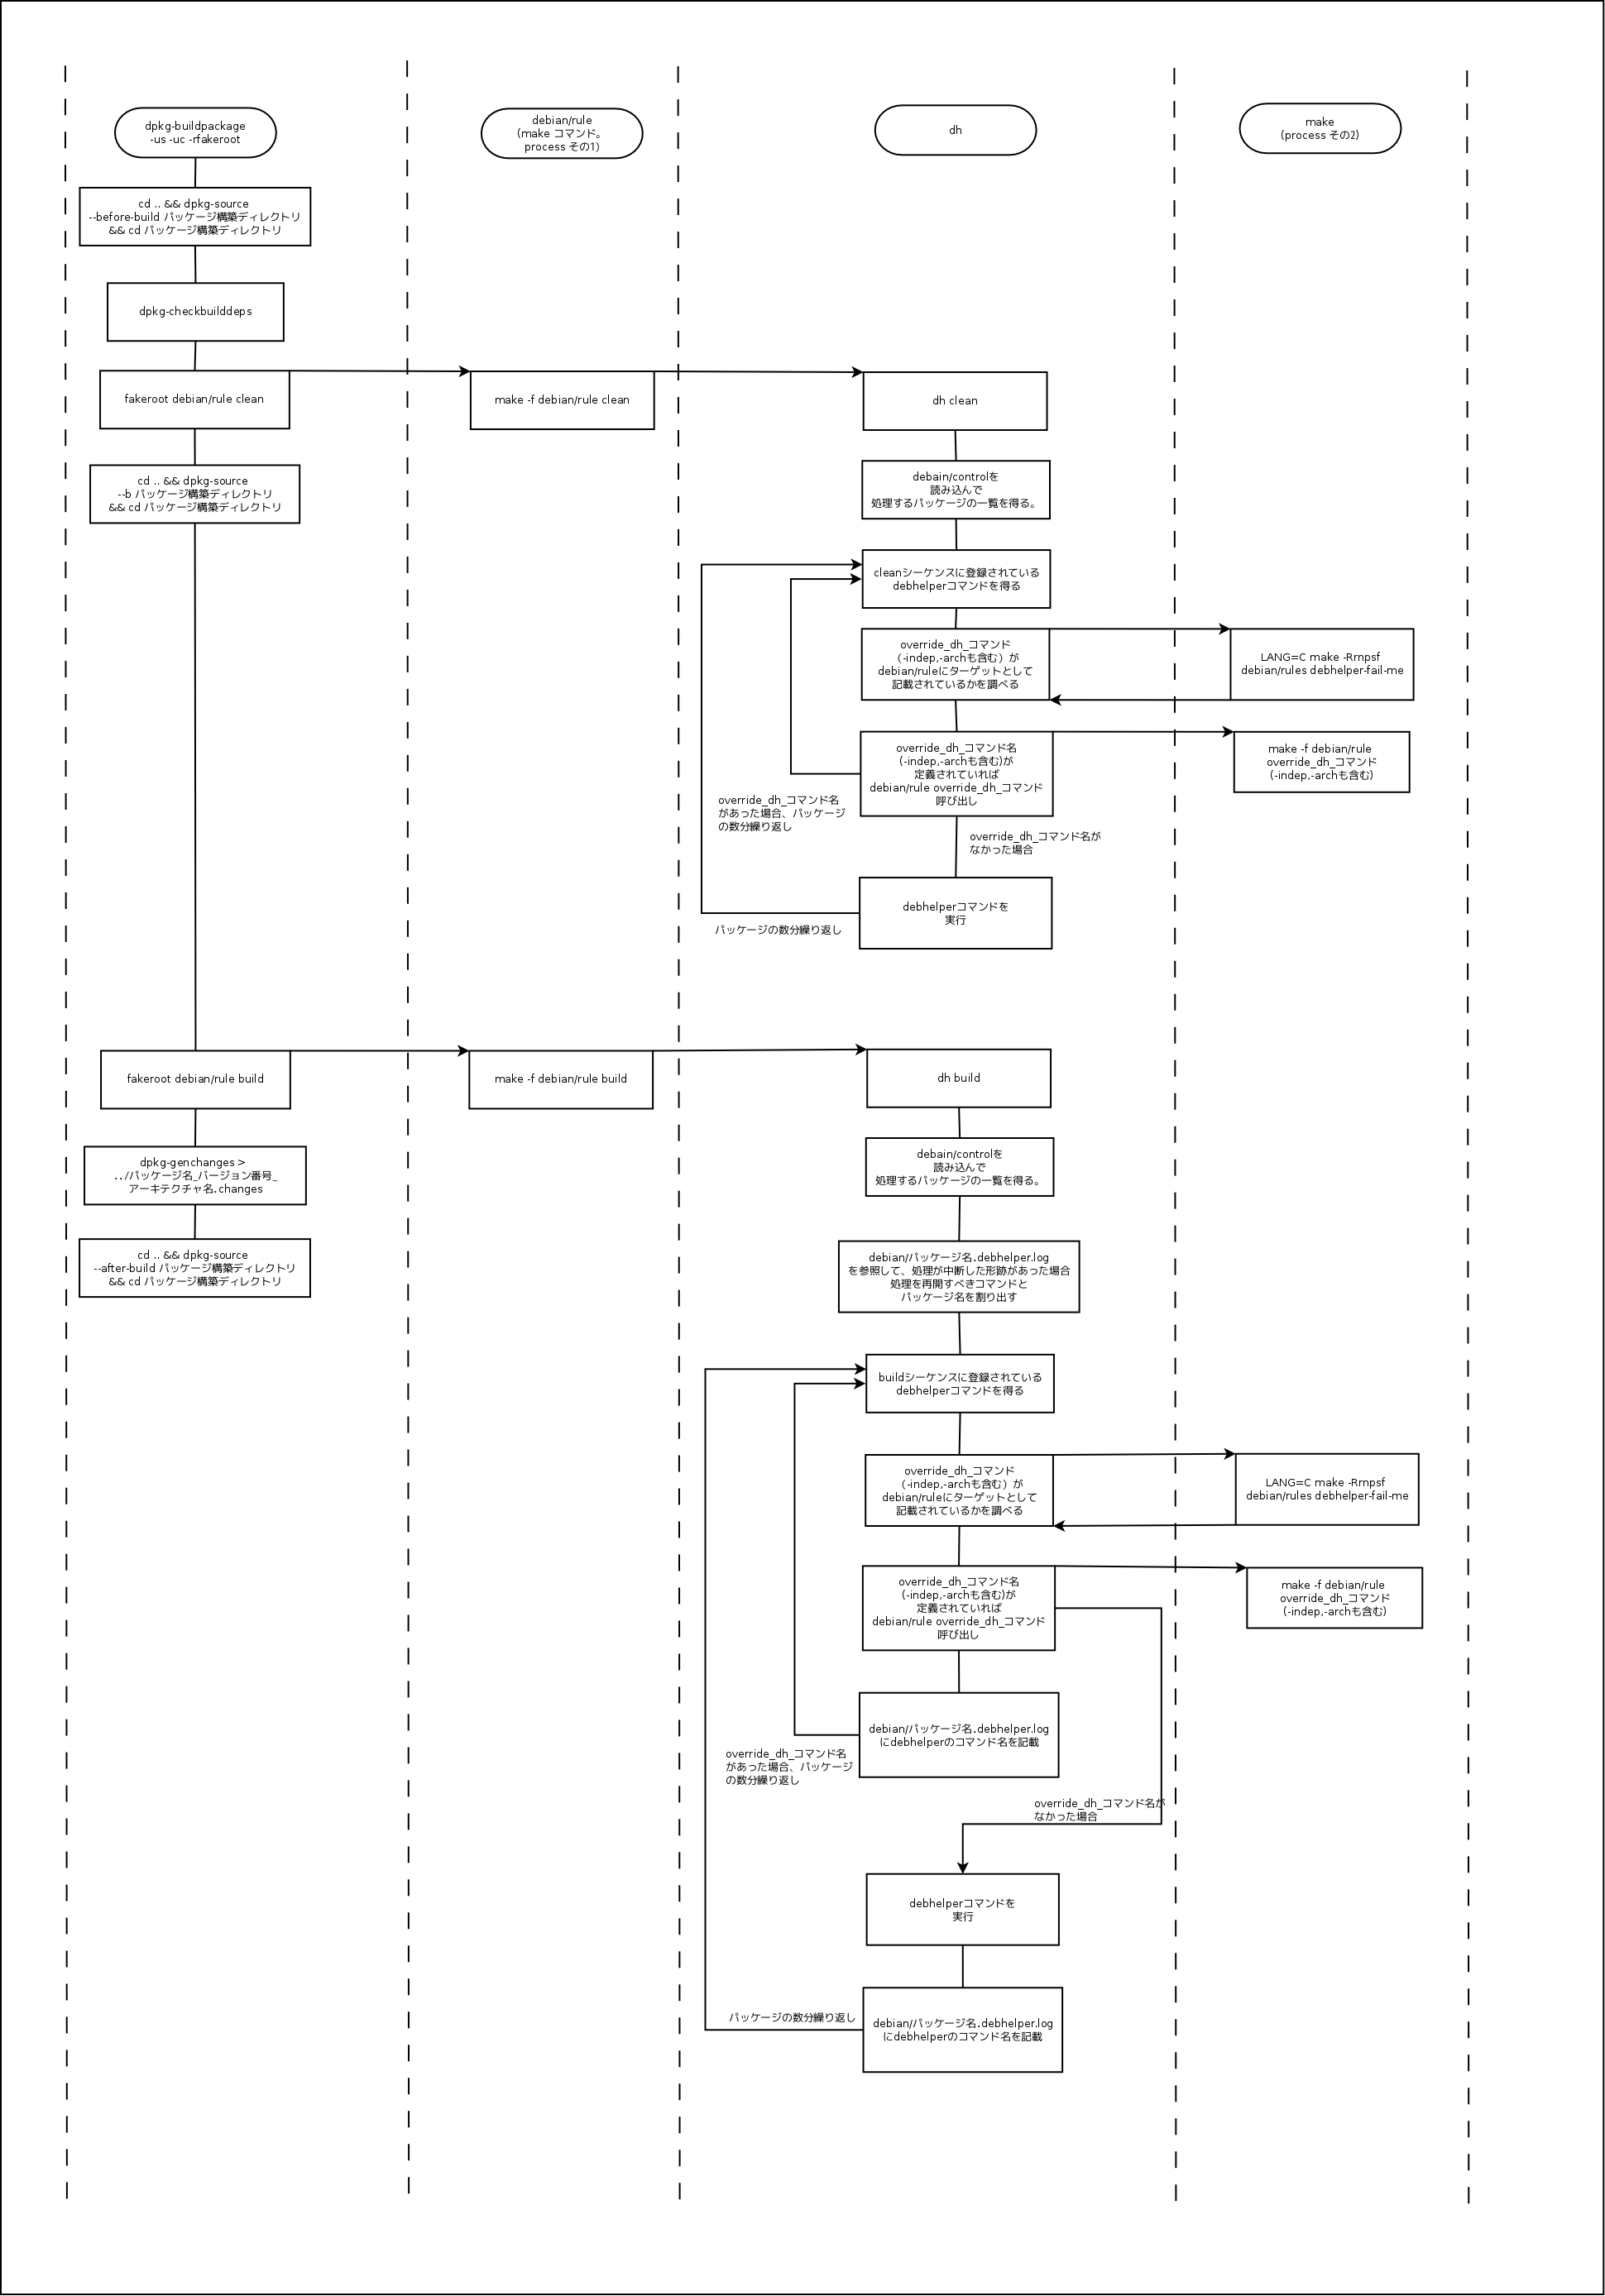
\includegraphics[width=17cm]{image201112/dh-internal-schema1.png}
  \end{center}
  \caption{dh$BFbItF0:n(B}
  \label{fig:dh-internal-schema1}
\end{figure}

$B?^(B\ref{fig:dh-internal-schema1}$B$+$iH=$k$h$&$K!"(Bdpkg-buildpackage$B$+$i(B
make$B%3%^%s%I$,5/F0$5$l!"<!$K(Bdh$B$,5/F0$5$l!"(B
$B$5$i$K(Bdh$B$+$i(Bmake$B$,5/F0$5$l$k$H$$$&4X78$K$J$C$F$$$k;v$,H=$j$^$9!#$^$?!"(B
override\_{\em debhelper$B%3%^%s%IL>(B}$B%?!<%2%C%H$N=hM}$r9T$&$N$K!"(Bmake$B%3%^%s%I$r;H$C$F(B
$B=hM}$r$7$F$$$k$H$$$&;v$bH=$j$^$9!#(B

dh$B$r;H$&$H!"(Bmake$B%3%^%s%I$O(Boverride\_{\em debhelper$B%3%^%s%IL>(B}$B%?!<%2%C%H$N=hM}$r$9$kLrL\$@$1$r(B
$BC4Ev$7$^$9!#(B
$B$=$N$&$A!"(Bdh$B%3%^%s%I$,?J2=$9$k$H!"(Bmake$B%3%^%s%I$NNO$r<Z$j$J$/$F$b%Q%C%1!<%8:n@.$,$G$-$k$h$&$K$J$k(B
$B$+$b$7$l$^$;$s$M!#(B

\subsubsection{``debian/$B%Q%C%1!<%8L>(B.debhelper.log''$B%U%!%$%k$K$D$$$F(B}

$B:G6a$N(Bdh$B%3%^%s%I$r;H$&(Bdebian/rules$B$K$O!"%U%!%$%k$N0MB84X78$K$D$$$F$N5-:\$,$"$j$^$;$s!#$3$N0Y!"%Q%C%1!<%8%S%k%ICf$G=hM}$,CfCG$7$?>l9g!"$I$3$+$i:F3+$9$l$PNI$$$+$r(Bdebian/rules$B$G(Bmake$B$,H=Dj$9$k;v$O$G$-$^$;$s!#(B

$B<B$O!"(Bdh$B%3%^%s%I$O(Bclean$B0J30$N%7!<%1%s%9$,;XDj$5$l$k$H!"(B''debian/$B%Q%C%1!<%8L>(B.debhelper.log''$B$H$$$&%U%!%$%k$K=hM}$r9T$C$?(Bdebhelper$B%3%^%s%I$r5-O?$7$F$$$^$9!#$3$3$G!"K|0l(Bdh$B$N=hM}$,CfCG$7$?>l9g!"=hM}$r$I$3$+$i;O$a$l$PNI$$$+$K$D$$$F$O$3$N%m%0%U%!%$%k$r;2>H$7$F=hM}$N:F3+$r9T$$$^$9!#(B

``debian/$B%Q%C%1!<%8L>(B.debhelper.log''$B$NCf?H$O0J2<$N$h$&$K$J$C$F$$$^$9!#(B

\begin{commandline}
debian/$B%Q%C%1!<%8L>(B.debhelper.log$B$NCf?H(B:
dh_auto_test
dh_prep
dh_installdirs
...$BCfN,(B...
dh_buiddeb
\end{commandline}

$B$^$?!"$3$N%U%!%$%k$O(Bdh clean$B$K$h$C$F>C5n$5$l$^$9!#$J$*!"(Bdh clean$B$N;~$K$O!"$3$N%m%0%U%!%$%k$O:n@.$5$l$^$;$s!#$D$^$j!"(Bdh clean$B$N=hM}$rCfCG$7$?>l9g$O!"(Bdh clean$B$O8F$S=P$5$l$k0lO"$N(Bdebhelper$B%3%^%s%I$O:G=i$+$i<B9T$5$l$F$7$^$$$^$9!#(B

$B$J$*!"=hM}:F3+$N>l=j$O!"$3$N%m%0%U%!%$%k$N$_;2>H$7$F7h$a$k0Y!"=hM}$rCfCG$7$?8e$K!"%Q%C%1!<%8$N%=!<%9%U%!%$%k$rJQ99$7$F:F3+$5$;$k$h$&$J;H$$J}$O$G$-$^$;$s!#Nc$($P!"%=!<%9%U%!%$%kCf$N$"$k%U%!%$%k$rJQ99$7$?0Y!"FCDj$N%Q%C%1!<%8$N%7!<%1%s%9$K$D$$$F$O:F2q;~$KA4It$d$jD>$7$,I,MW$@$C$?$H$7$F$b!"$3$l$r<+F0$G8!CN$9$k$3$H$O$G$-$^$;$s!#(B

\subsubsection{dpkg-buildflag$B$H$N4X78(B}

dh$B$O8_49@-EY9g$$(B(COMPATABLITY LEVEL)$B$N(Bv9$B$+$i!"(B
$B%Q%C%1!<%89=C[$N;~$K;H$&4D6-JQ?t$r@_Dj$9$k$?$a!"FbIt$G(Bdpkg-buildflag$BAjEv$N=hM}$r(B
$B8F$S=P$7$^$9!#(B

$B$=$N0Y!"(B9$B$r(Bdebian/compat$B$K;XDj$9$k$H!"(Bdebhelper$B%3%^%s%I$K@_Dj$5$l$k4D6-JQ?t$O!"(B
\begin{enumerate}
\item /etc/dpkg/buildflags.conf$B$NCf?H(B
\item XDG\_CONFIG\_HOME/dpkg/buildflags.conf (XDG\_CONFIG\_HOME$B$O4D6-JQ?t$G$9(B)$B$NCf?H(B
\item HOME/.config/dpkg/buildflags.conf (HOME$B$O4D6-JQ?t$G$9(B)$B$NCf?H(B
\item DEB\_flag\_MAINT\_SET, DEB\_flag\_MAINT\_STRIP, DEB\_flag\_MAINT\_APPEND, DEB\_flag\_MAINT\_PREPEND, DEB\_BUILD\_MAINT\_OPTINS$B!JA4It4D6-JQ?t$G$9!K$NCM(B
\end{enumerate}
$B$K$h$jMM!9$KJQ2=$7$^$9!#$I$N$h$&$KJQ$o$k$+$O(Bman dpkg-buildflag$B$r;2>H$7$F$/$@$5$$!#(B

\subsection{$B:#7n$N%3%^%s%I$=$N(B2:dh\_testroot}

\subsubsection{dh\_testroot$BF0:n>\:Y(B}

 $B8=:_$N<B9T%f!<%6$,(Broot$B$G$"$k$+$I$&$+$r3NG'$9$k%3%^%s%I$G$9!#(Broot$B%f!<%6$G$OL5$$>l9g!"(B
$B%(%i!<%a%C%;!<%8$r=PNO$7$F=hM}$rCfCG$7$^$9!#(B

\subsubsection{dh\_testroot$B%3%^%s%I%i%$%s%*%W%7%g%s(B}

$B!!%3%^%s%I%i%$%s%*%W%7%g%s$OFC$K$"$j$^$;$s!#2?$+;XDj$7$F$bL5;k$5$l$^$9!#(B

\subsubsection{dh\_testroot$B$r<B9T$7$F$_$k(B}

$BAaB.!"<B9T$7$F$_$^$7$g$&!#(B

\begin{commandline}
$ sudo dh_testroot
$ echo $?
0
$ dh_testroot
You must run this as root (or use fakeroot).
$ echo $?
255
$ fakeroot dh_testroot
$ echo $?
0
\end{commandline}
% $

$B$3$N$h$&$K(Broot$B8"8B$G<B9T$9$k$+!"(Bfakeroot$B7PM3$G<B9T$7$?;~$N$_(B0$B$rJV5Q$7$^$9!#(B

\subsubsection{$B<!2s$NH/I=$K$D$$$F(B}

$B<!$NH/I=<T$OJY6/2q$GH/I=$7$^$9!#A*$P$l$??M$O$h$m$7$/$*$M$,$$$7$^$9!#(B

\clearpage

%------------------------------------------------------------------------------
\dancersection{$B7n4)(Bdebhelper $BBh(B3$B2s(B}{$B;3ED(B $BBY;q(B}
%------------------------------------------------------------------------------
\index{$B$2$C$+$s$G$V$X$k$Q!<(B@$B7n4)(Bdebhelper}
\index{debhelper}

\subsection{$B$O$8$a$K(B}
$B%Q%C%1!<%8%S%k%I<j=g$r5-=R$9$k(Bdebian/rules$B%U%!%$%k!#$3$l$r(B
$B4J7i2=$9$k$?$a$K(Bdebhelper$B%3%^%s%I72(B(dh\_*)$B$,$"$j$^$9$,!"(B
$B$=$N0lJ}$GN"B&$G0lBN2?$,$J$5$l$F$$$k$N$+DO$_Fq$/$J$C$F(B
$B$7$^$$$^$7$?!#(B

$BK\4k2h$G$O$3$N%3%^%s%I72$r!"Kh7n;}$A2s$j$G2r@b$7$^$9!#Kh7n(B2$B$D0J>e$N(B
$B%3%^%s%I$r2r@b$7!"<!2sH/I=$NN)8uJd$,L5$$>l9g$OH/I=<T$,<!$NH/I=<T$r(B
$B;XL>$G$-$k$H$$$&%k!<%k$G?J$a$F9T$-$^$9!#(B

\subsection{$B:#7n$N%3%^%s%I!'(Bdh\&dh\_auto\_* - $B%7!<%1%s%9$H%S%k%I%7%9%F%`(B}

dh$B%3%^%s%I$NA4BNA|$K$D$$$F$OA02s$NLnEg$5$s$NH/I=$G4{$K2r@b$5$l$F(B
$B$$$k$N$G$9$,!"$=$3$G!V;n$7$KFI$s$G$_$k$H$h$$$H;W$$$^$9!W$H$"$C$?$N$G!"(B
$B<B:]$KFI$_$D$D$$$8$C$F$_$^$7$?!#$=$NCf$G$b$&>/$7H=$C$?$3$H$,$"$C$?$N$G(B
$BJs9p$7$^$9!#(B

\subsubsection{dh$B$NF0:n!":F$^$H$a(B}
\index{dh}

dh$B%3%^%s%I$r<B9T$9$k$H!"%G%U%)%k%H$G$O0J2<$N%3%^%s%I72$,(B
$B3F%7!<%1%s%9Kh$K8F$P$l$^$9!'(B

\begin{table}[ht]
\begin{center}
\small
\begin{tabular}{|p{8em}|p{35em}|}
\hline
$B%7!<%1%s%9L>(B&$B%7!<%1%s%9$G<B9T$5$l$k%3%^%s%I(B \\
\hline
clean & dh\_testdir dh\_auto\_clean dh\_clean \\
build & dh\_testdir + (rules build-arch build-indep) \\
build-indep & dh\_testdir dh\_auto\_configure dh\_auto\_build dh\_auto\_test \\
build-arch & dh\_testdir dh\_auto\_configure dh\_auto\_build dh\_auto\_test \\
install &
\begin{minipage}[t]{\columnwidth}%
(rules build install-arch install-indep) + \newline
dh\_testroot dh\_prep dh\_installdirs dh\_auto\_install
dh\_install dh\_install*\newline
dh\_bugfiles dh\_ucf dh\_lintian dh\_gconf dh\_icons
dh\_perl dh\_usrlocal dh\_link\newline
dh\_compress dh\_fixperms
\end{minipage} \\
install-indep & (rules install-indep) + $B!c>e$N(Binstall$B$HF1$8!d(B \\
install-arch & (rules install-arch) + $B!c>e$N(Binstall$B$HF1$8!d(B \\
binary & (rules install binary-arch binary-indep) \\
binary-indep &
\begin{minipage}[t]{\columnwidth}%
(rules install-indep) +
dh\_installdeb dh\_gencontrol dh\_md5sums dh\_builddeb \\
\end{minipage} \\
binary-arch &
\begin{minipage}[t]{\columnwidth}%
(rules install-arch) + \newline
dh\_strip dh\_makeshlibs dh\_shlibdeps + $B!c>e$N(Bbinary-indep$B$HF1$8!d(B \\
\end{minipage} \\
\hline
\end{tabular}
\caption{dh$B$N3F%7!<%1%s%9$G<B9T$5$l$k%3%^%s%I(B}
\label{tab:sequence-dh-commands}
\end{center}
\end{table}
$B$+$D$F$O(Brules(Makefile)$B$KMeNs$5$l$F$$$?%3%^%s%I72$,!"(B
$B:#$O(Bdh$B$NCf$K(BPerl$B$N%j%9%HJQ?t$G4IM}$5$l$F$$$k7A$K$J$j$^$9!#(B
$B$=$7$F(Bdebhelper$B%b%8%e!<%k!J(B*.pm$B!K$,%m!<%I;~$K%j%9%H$NFbMF$r(B
$B$$$8$C$F<B9TFbMF$rJQ99$9$k$3$H$G%S%k%I2aDx$r%+%9%?%^%$%:$7$^$9!#(B

$B$o$6$o$6(Bmake$B$r;H$o$:<+A0$J$N$O!"<B9TFbMF$rJQ99$9$k$H$$$&(B
$B%b%8%e!<%k5!9=$H(Boverride$B5!9=$,(Bmake$B%Y!<%9$G$O0MB84X78%D%j!<$N(B
$BJQ99$K$J$j<B8=:$Fq$@$C$?$+$i$G$7$g$&$+!#$?$7$+$K3HD%(Bmake$B$G$b(B
$B;H$o$J$$8B$jFq$7$=$&$G$9!J3HD%(Bmake$B$^$G9T$-$?$/$J$$$+$i8=>u$N(B
$B<B8=J}K!!&!&!&$J$s$G$7$g$&$+!K!#(B

$B$5$F!":#2s$NOCBj$O!"$3$N%b%8%e!<%k5!9=$K$J$j$^$9!#(B
$BIaCJ2?5$$J$/$I$s$J%Q%C%1!<%8$G$b%Q%C%1!<%8%S%k%I$5$l$F$$$kLu$G$9$,!"(B
$B8@8l4D6-$d3+H/<T$NA*Br$K$h$C$F%S%k%IJ}K!$O@i:9K|JL$G$9!#$3$l$O(B
$B$I$&$d$C$F5[<}$5$l$F$$$k$N$G$7$g$&$+!)(B

\subsubsection{$B#2$D$N%b%8%e!<%k!'%7!<%1%s%9$H%S%k%I%7%9%F%`(B}
$B$3$3$GEP>l$9$k$N$,!V%7!<%1%s%9!W$H$OJL$N!"!V%S%k%I%7%9%F%`!W(B
$B%b%8%e!<%k$K$J$j$^$9!#$3$N#2$D$O(B
\begin{itemize}
\item $B%7!<%1%s%9%b%8%e!<%k$O!J<g$K!KA0=hM}!&8e=hM}$rDI2C$7!"E,@Z$J%Q%C%1!<%8%S%k%I$,9T$o$l$k$h$&$K$9$k(B
\item $B%S%k%I%7%9%F%`%b%8%e!<%k$O3F%=!<%9%Q%C%1!<%8$KFbJq$5$l$k%S%k%IJ}<0$r<+F0G'<1$7!"$=$l$r6nF0$9$k(B
\end{itemize}
$B$H0[$J$kLr3d$r;}$A$^$9!#E57?E*$J(Bconfigure\&make$B%Q%?!<%s$G@bL@$9$k$H!"(B
\begin{enumerate}
\item Sequence/autotools\_dev.pm $B$,(B config.sub/config.guess $B$r:G?7$K99?7(B
\item Buildsystem/autoconf.pm $B$,(B ./configure $B$rH/8+!&<B9T(B
\item Buildsystem/makefile.pm $B$,(B Makefile $B$rG'<1$7!"(Bmake $B$G%S%k%I$d%$%s%9%H!<%k(B
\end{enumerate}
$B$H$$$C$?O"7H%j%l!<$K$J$j$^$9!J(Bautotools\_dev$B$O(B--with$B$GM-8z2=$5$l$?>l9g$N$_!K!#(B

\subsubsection{$B%S%k%I%7%9%F%`$NA*Br$HO"7H(B}
$B$5$F!"%S%k%I%7%9%F%`$O0J2<$N%U%m!<$G<+F0A*Br$5$l$F$$$^$9!'(B
\begin{enumerate}
\item $B$^$:!"(BBuildsystem/*.pm$B$OA4It%m!<%I$9$k(B
\item $B3F%b%8%e!<%k$N(Bcheck\_auto\_buildable API$B$K$F!V%S%k%I$G$-$kEY!W$r>H2q(B
\item $BF1$8%/%i%93,AX$NCf$G0lHVBg$-$$!V%S%k%I$G$-$kEY!W$rJV$7$?$b$N$rA*Br(B
\end{enumerate}
$B%]%$%s%H$O(B
\begin{itemize}
\item $B$3$N<+F0A*Br$O(Bconfigure/build/test/install/clean$B$N3FCJ$GKh2s9T$o$l$k(B
\item $BF1$8%/%i%93,AXG{$j$,$"$k(B
\end{itemize}
$B$N#2E@$G$9!#$D$^$j!"(B
\begin{itemize}
\item $BKh2s9T$o$l$k$N$G!"3FCJ$G1~Ez!&IT1~Ez$rJQ$($F%b%8%e!<%k4VO"7H$r9T$&(B
\item $B<+J,$,M%@h$5$l$k$Y$->l9g!"?F%/%i%9$N7k2L$r>e2s$k$h$&$K$7$F>!$D(B
\end{itemize}
$B$H$9$kI,MW$,$"$j!"!VC1=c$K%S%k%I$G$-$k$+$i??CM$rJV$9!W$H$$$&<BAu$G$O(B
$B$J$$$N$G$7$?!#$3$l$O<+A0$N%S%k%I%7%9%F%`3HD%!"FC$KB>$HO"7H$9$k>l9g$K(B
$BI,MW$JN10U;v9`$K$J$j$^$9!#6qBNE*$K$I$&$$$&%3!<%I$J$N$+$H$$$&$H(Bcmake$B$N(B
$B$b$N$,;29M$K$J$j$^$9!'(B
\begin{commandline}
=== Buildsystem/cmake.pm ===
sub check_auto_buildable {
    my $this=shift;
    my ($step)=@_;
    if (-e $this->get_sourcepath(``CMakeLists.txt'')) {
        my $ret = ($step eq ``configure'' && 1) ||
                  $this->SUPER::check_auto_buildable(@_);
        # Existence of CMakeCache.txt indicates cmake has already
        # been used by a prior build step, so should be used
        # instead of the parent makefile class.
        $ret++ if ($ret && -e $this->get_buildpath(``CMakeCache.txt''));
        return $ret;
    }
    return 0;
}
\end{commandline}
%$
Makefile$B%8%'%M%l!<%?$H$7$F(Bconfigure$B%9%F!<%8$@$1C4Ev$N$h$&$J(B
$B4i$r$7$D$D!"%S%k%I%-%c%C%7%e$,$"$k>l9g$O<+J,$,8eCJ$bC4Ev$9$Y$-$H$7$F(B
$B?F$G$"$k(Bmakefile.pm$B$r2!$7$N$1$F>!$D!"$H$$$&$o$1$G$9!#(B

\subsubsection{$B%S%k%I%7%9%F%`$OC/$,8F$s$G$$$k$N$+(B}
$B$H$3$m$G$3$N%S%k%I%7%9%F%`!"C/$,8F$s$G$$$k$N$G$7$g$&$+!)Nc$($P(Bdh$B$G$O(B
\begin{commandline}
$ dh --buildsystem=perl_makemaker
\end{commandline}
%$
$B$N$h$&$K;XDj$G$-$k$N$G$9$,!"(Bdh$B$K$O$I$3$K$b%S%k%I%7%9%F%`$K4X$9$k(B
$B=hM}$O=q$+$l$F$$$^$;$s!#(B

$B$3$l$O(Bdh$B$+$i%*%W%7%g%s$r$=$N$^$^%9%k!<%Q%9$5$l$k7A$G(B
\footnote{Debian$B$O!"%S%k%I%3%^%s%ID4::$N;~$b;W$$$^$7$?$,(B
$B%3%^%s%I%i%$%s0z?t$N0z$-2s$7K\Ev$KB?MQ$7$^$9$M!&!&!&(B}
dh\_auto\_(build\textbar{}clean\textbar{}configure\textbar{}install\textbar{}test)$B$N(B
dh\_auto\_*$B7O%3%^%s%I!J$@$1!K$,8F$S=P$785$K$J$C$F$$$^$9!#%7!<%1%s%9Cf$N(B
$B$9$Y$F$N(Bdh\_*$B%3%^%s%I$KF1MM$K%9%k!<%Q%9$OFO$/$N$G$9$,!"H?1~$9$k$N$,(B
$B$3$N(B5$B$D$@$1!"$H$$$&Lu$G$9!J(Bman debhelper$B$N(BBUILD SYSTEM OPTIONS$B!K!#(B
$B$@$+$i$3$=FH<+=hM}$r=q$/>l9g$O(Brules$B$K(B
\begin{commandline}
override_dh_auto_build:
        ...
\end{commandline}
$B$J$I$H(Boverride\_dh\_auto\_*$B%?!<%2%C%H$r=q$/$H$$$&OC$K$J$k$o$1$G$9!#(B
dh\_auto\_*$B$5$(;_$a$l$P!"$$$+$J$k%7!<%1%s%9$,Av$C$F$b%S%k%I%7%9%F%`(B
$B8F$S=P$7$,9T$o$l$:!"<B:]$N%S%k%I$O9T$o$l$J$$$+$i$G$9!#(B

$B$3$l$i$N(Bdh\_auto\_*$B%3%^%s%I$O>e$N%m!<%I"*>H2q(B(check\_auto\_buildable)\\
$B"*(BAPI(configure\textbar{}build\textbar{}test\textbar{}install\textbar{}clean)
$B%3!<%k$N%H%j%,$r0z$$$F$$$k$@$1$G$9!#$3$N%U%m!<$N>\:Y$O%i%$%V%i%j2=(B
$B$5$l$F$$$k$N$G3F%3%^%s%I$O(B3$B9T$/$i$$$7$+$"$j$^$;$s!#(B

\subsubsection{$B%S%k%I%7%9%F%`$NDI2CJ}K!(B}
$B%S%k%I%7%9%F%`$N3HD%$O4JC1$G!"0J2<$N(BAPI$B$r<BAu$7$?(B*.pm$B$r(BBuildsystem/
$B%U%)%k%@$KCV$/$@$1$G$9!#4pDl%/%i%9$K6u<BAu$,$"$k$N$GA4It=q$/I,MW$O$J$/!"(B
$B<B:]$K=hM}$rDI2C$7$?$$(BAPI$B$N$_<BAu$9$l$P==J,$G$9!#(B
\begin{quote}
\begin{verbatim}
check_auto_buildable($step)                          # $BI,?\(B
pre_building_step($step)                             # $B%*%W%7%g%s(B
configure() build() test() install($destdir) clean() # $B$$$:$l$+$r<BAu(B
post_building_step($step)                            # $B%*%W%7%g%s(B
\end{verbatim}
\end{quote}
$B3F(BAPI$B$N=hM}$OL>>N$+$iA[A|$5$l$kDL$j$G!"@h$K2r@b:Q$_$N(Bc\_a\_b API$B0J30$O(B
$BJVCM$b$"$j$^$;$s!J;H$o$l$F$$$^$;$s!K!#(B

$B%5%s%W%k$H$7$F!":#$O2{$+$7$-(Bimake/xmkmf$B$r;H$C$?%=!<%9%Q%C%1!<%8$N(B
$B<+F08!CN!\%S%k%I$KBP1~$9$k$h$&$K(Bimake.pm$B%b%8%e!<%k$rMQ0U$7$F$_$^$7$?!'(B
\begin{commandline}
package Debian::Debhelper::Buildsystem::imake;
use strict;
use base 'Debian::Debhelper::Buildsystem::makefile';

sub DESCRIPTION { "imake (IMakefile)" }
sub new { shift->SUPER::new(@_); }
sub check_auto_buildable {
    my($self, $step) = @_;
    return 1 if ($step eq "configure" &&
                 glob($self->get_sourcepath("I[Mm]akefile")));
    return 0;
}
sub configure { shift->doit_in_sourcedir("xmkmf", "-a", @_); }
1;
\end{commandline}
$B$3$s$J4JC1$J$b$N$G$b!"(Bkterm$B$J$I$NBP>]%Q%C%1!<%8$r%S%k%I$9$k$K$O==J,$G$9!#(B

$B$J$*!"$3$l$rAH$_9~$`$K$O(BDh\_Buildsystems.pm$B$N%=!<%9Cf$N<+F0H=Dj%j%9%H$N(B
$BKvHx$K(B
\begin{commandline}
our @BUILDSYSTEMS = (``autoconf'', ..., ``imake'');
\end{commandline}
$B$N$h$&$K%b%8%e!<%kL>$rDI2C$7$F$d$kI,MW$,$"$j$^$9!#(B

\subsubsection{$B$^$H$a(B}
$BK\2r@b$G$O(Bdh$B%U%l!<%`%o!<%/$r;Y$($k%S%k%I%7%9%F%`ItJ,$r2r@b$7$^$7$?!#(B
$B$3$l$O(Bdh\_*$B%3%^%s%I$H$7$F$O(Bdh\_auto\_*$B$N(B5$B%3%^%s%I$KBP1~$7!"$3$l$i$r(B
$BDL$7$F%S%k%I%7%9%F%`$,6nF0$5$l$F$$$^$9!#(B

\subsection{$B:#7n$N%3%^%s%I!'(Bdh\_builddeb}
\index{dh\_builddeb}

dh\_builddeb$B$O!"(Bdh$B$K$h$C$F5/F0$5$l$k0lO"$N%3%^%s%I%7!<%1%s%9$N:G8e$r(B
$B>~$k%3%^%s%I$G$9!J$A$J$_$K:G=i$O(Bdh\_testdir$B!K!#(B

$B%^%K%e%"%k$O!V(Bdpkg-deb $B$r8F$V$@$1$N$+$s$?$s$J$*$7$4$H(B\footnote{
dh\_builddeb simply calls dpkg-deb(1) to build a Debian package or packages.
}$B!W$H0l9T$@$1$N2r@b$G$9$,!"$3$l$,0U30$K$bCf$G?'!9$H$7$F$$$F(Bdh\_*$B%3%^%s%I$N(B
$BJY6/$K$J$j$^$9!#(B

\subsubsection{$B2?$r$7$F$$$k$N!)(B}

$B$d$C$F$$$k$3$H<+BN$O0J2<$N#3$D$G$9!'(B
\begin{enumerate}
\item debhelper(7)$B$N%U%!%$%kGS=|;XDj$,$"$l$P!"$=$N=|5n=hM}$r$9$k(B
\item deb/udeb$B7A<0$NH=Dj$r9T$$!"(Bdpkg-deb$B$N5/F0J,$1$r$9$k(B
\item $B$5$i$K!"(BDEB\_BUILD\_OPTIONS$B$N(Bparallel=$B;XDj$,$"$l$P!"(Bdpkg-deb$B$rJBNs6nF0$9$k(B
\end{enumerate}
$B%^%K%e%"%k$N2r@b$,#19T$N3d$K$O!"0U30$K;E;v$r$7$F$$$^$9!#(B

\subsubsection{$B5?Ld!'(Budeb$B$C$F2?!)(B}
\index{udeb}
$B<B$O(Budeb$B$NB8:_$rCN$j$^$;$s$G$7$?$,!"(Budeb$B$H$$$&$N$O(BDebian Installer(d-i)$B$G(B
$B;HMQ$5$l$k(B*.deb$BIw$N%Q%C%1!<%8$G$9!#7A<0$H$7$F$O(Budeb$B$b(Bdeb$B$bF1$8$G(B
$BIaDL$K(Bdpkg$B$GA`:n$G$-$k$N$G$9$,!"6K>.%j%=!<%9$G$N8BDjE*$JMxMQ$r(B
$BA[Dj$7$F$$$k$?$a%I%-%e%a%s%H$O$*$m$+%A%'%C%/%5%`5!G=$J$I$^$G30$5$l$F$$$^$9!#(B
\begin{commandline}
=== debian/control ===
Section: debian-installer
...
XC-Package-Type: udeb
XB-Installer-Menu-Item: 1200 <- d-i menu$B$G$NI=<(@)8f%Q%i%a!<%?(B
\end{commandline}
$B$N$h$&$KFC<l$J%X%C%@$,F~$C$F$$$k(Bcontrol$B$,$"$k>l9g!"(Bdh\_builddeb$B$O(B
$B<+F0E*$K(Budeb$B%S%k%I%b!<%I$G(Bdpkg-deb$B$r5/F0$7$^$9!#(B

$BB>$K$b$3$&$$$&FC<l%X%C%@$O$"$k$N$@$m$&$+$H$+!"$3$l$rF~$l$k$H(B
$B6qBNE*$K2?$r$I$&JQ$($i$l$k$N$+$J$I(Budeb$B$H(Bd-i$B$NOC$O99$K7!$k$H(B
$BLLGr$=$&$G$9$,!":#2s$OC&@~$H$$$&$3$H$G$3$3$^$G$K$7$F$*$-$^$9(B
\footnote{
$B;qNA$H$7$F$O(B http://d-i.alioth.debian.org/doc/talks/debconf6/paper/ $B$+$J!)(B
}$B!#(B
udeb$B8GM-=hM}$OB>$N(Bdh\_*$B%3%^%s%I$K$bB??t4^$^$l$F$*$j!"(Bis\_udeb()$B$G(B
$BMM!9$J=hM}J,$1$rN"B&$G$7$F$$$^$9!#(B

\subsubsection{debhelper(7)$B7O%3%^%s%I$N<BAu%Q%?!<%s(B}
dh\_builddeb$B$NCf$rGA$/$H!"3F=j$G(B\$dh{...}$B$H$$$&JQ?t$X$N%"%/%;%9$,(B
$BIQ=P$7$F$$$^$9!#$3$l$O(Bdh\_*$B%3%^%s%I$N(Bdebhelper(7)$B%*%W%7%g%s$N(B
$B%Q!<%9$d6&DLE*$J=hM}$,(B Debian::Debhelper::Dh\_Lib $B%i%$%V%i%j$G(B
$B9T$o$l$F$*$j!"$3$N%i%$%V%i%j$H%3%^%s%IB&$NO"7H$K(B \%dh $B$H$$$&(B
$B%0%m!<%P%kJQ?t$,;H$o$l$F$$$k$?$a$G$9!#$^$?(B \%ENV $B$bB?MQ$5$l$F$$$^$9!#(B

$B%3!<%I$NN.$l$H$7$F$O!"(Bdebhelper$B$N=c@5(B(Perl$B@=(B)dh\_*$B%3%^%s%I$O(B
$B35$M0J2<$N<BAu%Q%?!<%s$K$J$C$F$$$^$9!'(B

\begin{commandline}
use Debian::Debhelper::Dh_Lib; # init()$B4X?t$J$I$,%$%s%]!<%H$5$l$k(B
init(options => { ``myopt=s'' => \&dh{MYOPT}, ... }); # @ARGV$B$d(B%ENV$B$NDj7?=hM}(B

# $B4^$^$l$F$$$k%Q%C%1!<%8$N?t$@$1=hM}$rH?I|(B
foreach my $package (@{$dh{DOPACKAGES}}) {
    # $B>e$N(Binit()$B$G<h$j9~$^$l$?7k2L$r8+$J$,$i=hM}$r$9$k(B
    if ( $dh{...}) { ... # Dh_Lib.pm $B$N(B API $B$r8F$s$@$j$9$k$J$I(B ... }
    # $B<+F0E*$K<h$j9~$^$l$J$$4D6-JQ?t!J%3%^%s%I8GM-!K$O<+J,$G=hM}$9$k(B
    if ($ENV{...}) { ... # $B>e5-F1MM(B ... }
}
\end{commandline}

dh\_builddeb$B$N>l9g$O!">e$N%k!<%W$NCf$,ITMW%U%!%$%k$N:o=|$H(B
dpkg-deb$B$N5/F0$K$J$j!"$3$l$,Nc$($P(Bdh\_strip$B$N>l9g$O3F@8@.Cf%Q%C%1!<%8$N(B
$B%o!<%-%s%0%U%)%k%@$r%9%-%c%s$7$F!"$7$+$k$Y$-%U%!%$%k$r(Bstrip$B$7$F2s$k$H(B
$B$$$&$h$&$K$J$j$^$9!#(B

\subsubsection{$B$^$H$a(B}
dh\_builddeb$B%3%^%s%I$N2r@b$H!"$=$3$+$i=P$F$-$?5?Ld$H6&DLE*$J9=@.$N2r@b$r(B
$B9T$C$F$_$^$7$?!#(Bdh\_*$B%3%^%s%I$O<B<A#19T$7$+$J$$$b$N$+$i(B1000$B9T$KGw$k$b$N$^$G(B
$B?'!9$"$j$^$9$,!"(Bdh\_builddeb$B$O$A$g$&$IM}2r$9$k>e$G<j:"$JBg$-$5$G$9!#(B

\clearpage

%-------------------------------------------------------------------------------
\dancersection{$B7n4)(Bdebhelper $BBh(B4$B2s(B}{$B;3K\(B $B9@G7(B}
%-------------------------------------------------------------------------------
\index{$B$2$C$+$s$G$V$X$k$Q!<(B@$B7n4)(Bdebhelper}
\index{debhelper}

\subsection{$B%Q%C%1!<%8$N(Bmake$B$NA0$K!D(B}

$B@h7n$^$G$K3X$s$G$-$?$h$&$K!"(Bdebhelper $B$O!"4pK\E*$K%S%k%I$KI,MW$J0lO"$N(Bdh\_XXX $B%3%^%s%I$r<+F0<B9T$7$^$9!#(B

$BNc$($P(Bdebhelper$B$O!"(Bdh\_auto\_configure$B$H$$$&%3%^%s%I$rDs6!$7$F$*$j!"$3$l$O$4A[A|$NDL$j!"(B
\begin{commandline}
./configure --build='dpkg_architecture_value("DEB_BUILD_GNU_TYPE")' --prefix=/usr --includedir=/usr/include \
--mandir=/usr/share/man --infodir=/usr/share/info --sysconfdir=/etc --localstatedir=/var \
--libdir=/usr/lib/\$multiarch --libexecdir=/usr/lib/\$multiarch --disable-maintainer-mode \
--disable-dependency-tracking --host='dpkg_architecture_value("DEB_HOST_GNU_TYPE")
\end{commandline}
$B$r$7$F$$$k$@$1$G$9!#(B

$B$7$+$7!"%a%s%F%J$K$h$C$F(Bautotools$B$rMxMQ$7!"(Bconfugure$B%9%/%j%W%H$r%S%k%I$NEY$KKh2s(Bconfigure.ac$B$+$i@8@.$7$?$$?M$b$$$k$G$7$g$&$7!"$b$7$+$9$k$H(BMakefile$B$N85$H$J$k(BMakefile.in$B$@$C$F!"Kh2s(BMakefile.am$B$+$i@8@.$7$?$$?M$b$$$k$G$7$g$&!#(B
$B$^$?!"(BDebian$B%Q%C%1!<%8%*%j%8%J%k$N%Q%C%A$r$"$F$F%Q%C%1!<%8$r:n$k$N$O!"$4$/Ev$?$jA0$N$h$&$K9T$J$o$l$F$$$^$9!#(B

$B$=$3$G:#7n$O!"0lO"$N(Bdh\_XXXX$B%3%^%s%I$X$NDI2C$N;EAH$_$H!"$=$NNc$H$7$F!"(Bdpatch$B%Q%C%1!<%8$GDs6!$5$l$k(Bdh\_dpatch\_patch$B%3%^%s%I$H!"(Bautotools-dev$B%Q%C%1!<%8$GDs6!$5$l$k(Bdh\_autotools-dev\_updateconfig$B%3%^%s%I$NDI2C$K$D$$$F2r@b$7$^$7$g$&!#(B

\subsection{$B0lO"$N(Bdh\_XXXX$B%3%^%s%I$X$NDI2C$N;EAH$_(B}

$B4pK\$H$J$k0lO"$N(Bdh\_XXXX$B%3%^%s%I$O!"Bg85$N%3%^%s%I$G$"$k(Bdh$B%9%/%j%W%H$K5-=R$7$F$"$j!"$9$Y$F$K$D$$$F$O@h7n$d@h!97n$KOC$5$l$F$$$k$N$G!"3d0&$7$^$9!#(B

$BFC$K(Bmake$BD>A0$K<B9T$5$l$k$b$N$O!"(B
\begin{commandline}
dh_testdir  #$B%+%l%s%H%G%#%l%/%H%j$N3NG'(B
dh_auto_configure  #./configure$B$N<B9T(B
\end{commandline}
$B$@$1$G$9!#(B

$BL^O@!"$3$l$@$1$G$O%Q%C%A$b$"$F$i$l$J$$$G$9$7!"(Bconfigure$B%9%/%j%W%H$N:F@8@.$b$G$-$^$;$s!#(B

$B$=$3$G(Bdh$B%9%/%j%W%H$O!"0lO"$N(Bdh\_XXX$B%3%^%s%I$rNs5s$9$kG[Ns$K$7!"$3$l$r(B\$sequences{\$sequence}$B$N%9%+%iJQ?t$H$7$FJ];}$7$F$$$^$9!#(B($B$3$NJU$O(Bperl$B$K$"$^$j>\$7$/$J$$$N$G!"$A$g$C$H4V0c$C$F$$$k$+$b!D(B)

$B$^$?!"$3$N(B\$sequences$B$+$i(Bdh\_XXXX$B%3%^%s%I$r=|$$$?$j(B(remove\_command)$B!"$"$k(Bdh\_XXXX$B%3%^%s%I$NA0$KDI2C$9$k(B(insert\_before)$B%5%V%k!<%A%s$bMQ0U$5$l$F$$$^$9!#(B

dh$B%9%/%j%W%H$O!"(B/usr/share/perl5/Debian/Debhelper/Sequence/$B%G%#%l%/%H%j$N$J$+$K$"$k%U%!%$%k$r;2>H$7$F$*$j!"$3$3$K(B
\begin{commandline}
insert_before("dh_auto_configure", "dh_new_command")
\end{commandline}
$B$H$$$&5-=R$N$"$k%U%!%$%k(B($B%"%I%*%s(B)$B$,DI2C$5$l$k$H!"(Bdh\_auto\_configure$B$NA0$K(Bdh\_new\_command $B$,<B9T$5$l$k$h$&$K$J$j$^$9!#(B

$B$?$@$7!"(Brules$B$N(B
\begin{commandline}
dh $@ --with $B!A(B
\end{commandline}
%$
$B$G%"%I%*%s$,;XDj$5$l$J$$8B$jI>2A$O$5$l$J$$$N$G!"%S%k%I$KITI,MW$J(Bdh\_XXXX$B%3%^%s%I$rF~$l$F$$$F$bBg>fIW$J$O$:$G$9!#(B

\subsection{dh\_dpatch\_patch$B%3%^%s%I(B}

dpatch$B%Q%C%1!<%8$r%$%s%9%H!<%k$9$k$H!"(B/usr/share/perl5/Debian/Debhelper/Sequence/$B%G%#%l%/%H%j$K(Bdpatch.pm$B%U%!%$%k$,F~$j!"$3$l$K$O!"(B
\begin{commandline}
insert_before("dh_auto_configure", "dh_dpatch_patch")
insert_before("dh_clean", "dh_dpatch_unpatch")
\end{commandline}

$B$H$$$&5-=R$,$"$j$^$9!#$3$l$O8+$FA[A|$G$-$k$H$*$j!"(Bmake$B$ND>A0$K<B9T$5$l$k(B./configure$B$N$5$i$KD>A0$K!"(Bdh\_dpatch\_patch$B$r2C$($F$$$^$9!#(B
$B$^$?!"2<$N5-=R$O!"0JA0$K%S%k%I$7$?$3$H$,$"$k>l9g$K!"%Q%C%A$9$kA0$N>uBV$K$9$k(Bdh\_dpatch\_unpatch$B%3%^%s%I$bDI2C$5$l$F$$$^$9!#(B

$B$3$N(Bdh\_dpatch\_patch$B$O!"%Q%C%1!<%8%=!<%9$N(Bdebian/patches/00list$B$K5-=R$5$l$?%U%!%$%kL>$N%Q%C%A$r@hF,$+$i%Q%C%A$9$k%3%^%s%I!"(Bdpatch$B%9%/%j%W%H$r<B9T$7$^$9!#(B

$B$9$J$o$A!"$b$7(Bconfigure$B%9%/%j%W%H$K(Bdpatch$B$G$J$s$i$+$N%Q%C%A$r$"$F$F<B9T$7$?$1$l$P!"(Bdpatch$B%Q%C%1!<%8$r(BBuild-dep$B$7!"(Bdebian/patches/$B%G%#%l%/%H%j$K%Q%C%A%U%!%$%k$H$=$l$K9g$o$;$?(B00list$B%U%!%$%k$rMQ0U$7!"(B
\begin{commandline}
dh $@ --with dpatch
\end{commandline}
$B$H(Brules$B%U%!%$%k$K5-=R$7$F$*$1$PNI$$$O$:$G$9!#(B

make$B$@$1$7$?$$$J$i$P!"%?!<%_%J%k$G!"(B
\begin{commandline}
$ dh_dpatch_patch
$ ./configure $B!A(B
$ make
\end{commandline}
%$
$B$G$bBg>fIW$G$9!#(B

\subsection{autotools$B$@$C$F;H$$$?$$(B}

$B%S%k%I$9$k%^%7%s$N4D6-$K9g$o$;$F!"(Bconfigure$B%9%/%j%W%H$J$I$rD4@0$7$F$/$l$k%D!<%k$H$7$F!"(BGNU autotools$B$H$$$&$b$N$,$"$j$^$9!#<!$K$3$N(BGNU autotools$B$r(Bdebhelper$B$GMxMQ$9$kJ}K!$K$D$$$F=R$Y$^$7$g$&!#(B

\index{dh-autoreconf}
dh-autoreconf$B%Q%C%1!<%8$r%$%s%9%H!<%k$9$k$H!"0MB84X78$G(Bautomake$B!"(Bautoconf$B$H!"(Bautomake$B$K0MB8$7$F(Bautotools-dev$B$,%$%s%9%H!<%k$5$l$^$9!#(B
autotools-dev$B%Q%C%1!<%8$O(B\\
/usr/share/perl5/Debian/Debhelper/Sequence/$B%G%#%l%/%H%j$K(Bautotools-dev.pm$B%U%!%$%k$,F~$j$^$9!#(B
$B$3$l$K$O!"(B
\begin{commandline}
insert_before("dh_auto_configure", "dh_autotool-dev_updateconfig")
insert_before("dh_clean", "dh_autotool-dev_restoreconfig")
\end{commandline}
$B$H5-=R$5$l$F$$$^$9!#(B

dh\_autotool-dev\_updateconfig$B%3%^%s%I$O!"%+%l%s%H%G%#%l%/%H%j0J2<$G<B9T$7$F$$$k%7%9%F%`%?%$%W$NI8=`L>$r?dB,$9$k$?$a$N(Bconfig.guess$B$H(Bconfig.sub$B%U%!%$%k$rC5$7!"(Bconfig.guess.dh-orig$B$H(Bconfig.sub.dh-orig$B%U%!%$%k$KL>A0$r49$(!"$=$l$>$l(B/usr/share/misc/$B%G%#%l%/%H%j$K$"$k:G?7(Bautotool-dev$B$N(Bconfig.guess$B$H(Bconfig.sub$B$r%3%T!<$7$F$-$^$9!#(B

dh-autoreconf$B%Q%C%1!<%8$O(B/usr/share/perl5/Debian/Debhelper/Sequence/$B%G%#%l%/%H%j$K(Bautoreconf.pm$B%U%!%$%k$,F~$j$^$9!#(B
$B$3$l$K$O!"(B
\begin{commandline}
insert_before("dh_auto_configure", "dh_autoreconf")
insert_before("dh_clean", "dh_autoreconf_clean")
\end{commandline}
$B$H5-=R$5$l$F$$$^$9!#(B

dh\_autoreconf$B%3%^%s%I$O!"4JC1$K8@$&$H!"(Bautomake$B!"(Bautoconf$B$r$7$F$/$l$k(Bautoreconf$B%9%/%j%W%H$r8F$S=P$7!"(Bconfigure$B$d(BMakefile.in$B$r:F@8@.$7$^$9!#(B

dh\_autoreconf$B$r;H$$$?$$$H$-$O!"$3$N%Q%C%1!<%8$K(BBuild-dep$B$7!"(B
\begin{commandline}
dh $@ --with autoreconf
\end{commandline}
%$
$B$H(Brules$B%U%!%$%k$K5-=R$7$F$*$1$PNI$$$O$:$G$9!#(B
debian/autoreconf$B%U%!%$%k$K%G%#%l%/%H%j$N%j%9%H$,$"$l$P!"$=$3$@$1(Bconfigure$B$d(BMakefile.in$B$r99?7$7$F$/$l$^$9!#(B

autoreconf.pm$B%U%!%$%k$G$O!V(Bdh\_auto\_configure$B$h$jA0$@$h!W$H$$$&;XDj$7$+$"$j$^$;$s$+$i!"(Bdh\_autoreconf$B$,<B9T$5$l$F%Q%C%A$,$"$F$i$l$k$N$+!"%Q%C%A$,$"$F$i$l$F$+$i(Bdh\_autoreconf$B$,<B9T$5$l$k$N$+$^$G$O5-=R$5$l$F$$$^$;$s!#(B
dh$B%9%/%j%W%H$r8+$?8B$j$G$O!V(B--with$B!W%*%W%7%g%s$N=g$G%j%9%H$5$l$F$$$k$h$&$G$9!#$D$^$j!"(Bdh-autoreconf$B%Q%C%1!<%8$rMxMQ$9$k%=!<%9%Q%C%1!<%8$N(BMakefile$B$KBP$7$F(BBTS$B$G%Q%C%A$r=q$/>l9g$O!"!V(B--with$B!W%*%W%7%g%s$N=g$r3NG'$9$kI,MW$,$"$j$=$&$G$9!#(B

\subsection{$B$*$o$j$K(B}

$B:#2s$O(Bmake$B$r<B9T$9$kA0$K;HMQ$5$l$k(Bconfigure$B%9%/%j%W%H$J$I$N!"(Bdebhelper$B$r;H$C$?%+%9%?%^%$%:K!$K$D$$$F!"6n$1B-$G@bL@$7$F$_$^$7$?!#(B

\clearpage

%-------------------------------------------------------------------------------
\dancersection{$B7n4)(Bdebhelper $BBh(B5$B2s(B}{$B?yK\(B $BE5=<(B}
%-------------------------------------------------------------------------------
\index{$B$2$C$+$s$G$V$X$k$Q!<(B@$B7n4)(Bdebhelper}
\index{debhelper}


\subsection{$B:#7n$N%3%^%s%I!'(Bdh\_md5sums}
\index{dh\_md5sums}

dh\_md5sums$B%3%^%s%I$O!V(BDEBIAN/md5sums$B%U%!%$%k$r@8@.$9$k!W%3%^%s%I$G$9!#(B

\subsubsection{DEBIAN/md5sums$B%U%!%$%k$K$D$$$F(B}
$B!V(B\$ ar x debian-package.deb$B!W$r<B9T$78=$l$k(Bcontrol.tar.xx$B%U%!%$%k$rE83+(B
$B$9$k$H(Bmd5sums$B%U%!%$%k$,=P$F$-$^$9!#$3$N(Bmd5sums$B%U%!%$%k$O(Bdata.tar.xx$B%U%!%$%k$K4^$`%U%!%$%k$=$l$>$l$+$i<hF@$7$?(Bmd5sum$B$r5-=R$7$F$$$^$9!#(B

\begin{commandline}
$ apt-get download hello-debhelper
$ ar x hello-debhelper_2.7-3_i386.deb
$ ls
control.tar.gz  data.tar.gz  debian-binary  hello-debhelper_2.7-3_i386.deb
$ tar xf control.tar.gz
$ ls
control         data.tar.gz    hello-debhelper_2.7-3_i386.deb
control.tar.gz  debian-binary  md5sums
$ head -n 1 md5sums
098518cc321f0467dc0e7c67f65e2cc1  usr/bin/hello
\end{commandline}
%$

\subsubsection{$B%Q%C%1!<%8$N%S%k%I=hM}$K$*$1$k(Bdh\_md5sums$B$N<B9T(B}
dh\_md5sums$B%3%^%s%I$O%$%s%9%H!<%k$9$k%U%!%$%k$N(Bmd5sum$B$r<hF@$9$k=hM}$N$?$a!"%S%k%I=hM}$N=*HW$G<B9T$5$l$^$9!#(B

\begin{commandline}
$ apt-get source hello-debhelper
$ cd hello-debhelper-2.7
$ debuild -uc -us
  ($B>JN,(B)
  dh\_gencontrol -a
  dh\_md5sums -a
  dh\_builddeb -a
  ($B>JN,(B)
$ ls debian/hello-debhelper
DEBIAN   usr
$ head -n 1 debian/hello-debhelper/DEBIAN/md5sums
098518cc321f0467dc0e7c67f65e2cc1  usr/bin/hello
\end{commandline}
%$

\subsubsection{$B%3%^%s%I$N%*%W%7%g%s(B}

\begin{table}[ht]
\caption{dh\_md5sums$B$N%3%^%s%I%i%$%s%*%W%7%g%s0lMw(B}
\begin{center}
\small
\begin{tabular}{|p{12em}|p{33em}|}

\hline
$B%*%W%7%g%s(B&$B@bL@(B \\
\hline
-x,  --include-conffiles & DEBIAN/conffiles$B%U%!%$%k$K5-=R$7$?@_Dj%U%!%$%k$N(Bmd5$B$b@8@.$7$^$9!#(B\\
\hline
-Xitem, --exclude=item & md5sum$B$N@8@.$r=|30$9$k%U%!%$%kL>$r;XDj$7$^$9!#$?$@$7%G%#%l%/%H%j$,JL$G$b%U%!%$%kL>$,0lCW$9$l$P$I$A$i$b=|30$5$l$^$9!#(B \\
\end{tabular}
\end{center}
\end{table}

\subsection{$B:#7n$N%3%^%s%I!'(Bdh\_strip}
\index{dh\_strip}

dh\_strip$B%3%^%s%I$O!V<B9T%U%!%$%k!"6&M-%i%$%V%i%j!"%9%?%F%#%C%/%i%$%V%i%j$r(Bstrip$B$9$k!W%3%^%s%I$G$9!#(B

\subsubsection{$B%G%P%C%0%7%s%\%k$N07$$J}$r@)8f$9$k(B}
$B%*%W%7%g%s$J$7$d4D6-JQ?t$r;XDj$;$:$K(Bdh\_strip$B%3%^%s%I$r<B9T$9$k$H%3%s%Q%$%k$7$?%*%V%8%'%/%H%U%!%$%k$N%G%P%C%0%7%s%\%k$r(Bstrip$B$9$k$N$,DL>o$N=hM}$G$9!#$7$+$7!"%G%P%C%0$rL\E*$H$9$k>l9g$O%G%P%C%0%7%s%\%k$r(Bstrip$B$7$F$7$^$&$H%G%P%C%,$,==J,$K5!G=$7$J$$$?$a:$$j$^$9!#(B

dh\_strip$B%3%^%s%I$G$O%G%P%C%0%7%s%\%k$r0J2<$N$h$&$K07$&$3$H$,$G$-$^$9!#(B\cite{debugpackage}

\begin{itemize}
 \item $B%*%W%7%g%s$J$7$G<B9T$9$k$H!"(Bstrip$B$9$k!#(B
 \item $B4D6-JQ?t(BDEB\_BUILD\_OPTIONS=nostrip$B$r;XDj$7$F<B9T$9$k$H!"(Bstrip$B$7$J$$!#!J=hM}E*$K$O(Bdh\_strip$B$,B(:B$K=*N;$9$k!K(B
 \item --dbg-package$B%*%W%7%g%s$r;XDj$9$k$H!"(B/usr/lib/debug$BG[2<$K%G%P%C%0%7%s%\%k$rJ,N%$7$F;D$9%Q%C%1!<%8!J!a%G%P%C%0%Q%C%1!<%8!K$r:n@.$9$k!#(B
\end{itemize}

\subsubsection{$B%G%P%C%0%Q%C%1!<%8$r:n@.$9$k$?$a$N>r7o(B}
debhelper$B$N5!G=$rMxMQ$9$k$H(Bstrip$B:Q$_$N%P%$%J%j%Q%C%1!<%8$K2C$($F4JC1$K%G%P%C%0%Q%C%1!<%8$r:n@.$G$-$^$9!#%G%P%C%0%Q%C%1!<%8$rDI2C$G:n@.$7$?$$>l9g$O0J2<$N=hM}$r5-=R$7$F%Q%C%1!<%8$r%S%k%I$9$l$P$h$$$G$9!#(B

\begin{itemize}
 \item CFLAGS$B$J$I$N%3%s%Q%$%k%*%W%7%g%s$K(B''-g'$B$rIUM?$7%S%k%I;~$K%G%P%C%0%7%s%\%k$r@8@.$9$k$h$&$K$9$k!#(B
 \item debian/rules$B$G(Boverride\_dh\_strip$B$rDj5A$7!"(Bdh\_strip --dbg-package=package-dbg$B$r=hM}$5$;$k!#(B
 \item debian/control$B$K%Q%C%1!<%8!V(Bpackage-dbg$B!W$NDj5A$r5-=R$9$k!#$3$N$H$-!"%Q%C%1!<%8!V(Bpackage-dbg$B!W$O%Q%C%1!<%8!V(Bpackage$B!W$K%P!<%8%g%s;XDj$r$7$F(Bdepend$B$9$k$3$H!#(B
\end{itemize}

\subsubsection{$B%3%^%s%I$N%*%W%7%g%s(B}

\begin{table}[ht]
\caption{dh\_strip$B$N%3%^%s%I%i%$%s%*%W%7%g%s0lMw(B}
\begin{center}
\small
\begin{tabular}{|p{12em}|p{33em}|}
\hline
$B%*%W%7%g%s(B&$B@bL@(B \\
\hline
-Xitem, --exclude=item & $B;XDj$7$?J8;zNs$r4^$`%U%!%$%k$r(Bstrip$B=hM}$NBP>]$+$i=|30$9$k!#J#?t$N%U%!%$%k$r;XDj$7$?$$>l9g$O%*%W%7%g%s$rJ#?t2s;XDj$9$k$3$H$b2DG=!#(B\\
\hline
--dbg-package=package & $B%G%P%C%0%7%s%\%k$r4^$`%Q%C%1!<%8!V(Bpackage-dbg$B!W$r:n@.$9$k!#(B \\
\hline
-k, --keep-debug & $B%Q%C%1!<%8$r%S%k%I$7$?:n6H%G%#%l%/%H%jFb$N(Busr/lib/debug$B$K(Bstrip$B8e$N%G%P%C%0%7%s%\%k%U%!%$%k$r;D$9!#(B--dbg-package$B%*%W%7%g%s$N;XDj$G;vB-$j$k>l9g$OB?$$$,!"$h$j:Y$+$/%G%P%C%0%7%s%\%k$r07$$$?$$>l9g$rA[Dj$7$FMQ0U$5$l$F$$$k!#(B \\
\end{tabular}
\end{center}
\end{table}

\begin{thebibliography}{0}
\bibitem{debugpackage} Debian Wiki - DebugPackage \url{http://wiki.debian.org/DebugPackage}\
\bibitem{bestpkgpractice} Debian.org $BBh(B6$B>O%Q%C%1!<%82=$N%Y%9%H%W%i%/%F%#%9(B \url{http://www.debian.org/doc/manuals/developers-reference/best-pkging-practices.html}
\end{thebibliography}

\clearpage

%-------------------------------------------------------------------------------
\dancersection{Debian$B3+H/<T$N(BKDE$B4D6-$"$l$3$l(B}{$BLnEg(B $B5.1Q(B}
%-------------------------------------------------------------------------------
\index{Debian$B$+$$$O$D$7$c$N(BKDE$B$+$s$-$g$&(B@Debian$B3+H/<T$N(BKDE$B4D6-(B}
\index{kde}

$B:G6a$N(BDebian$B$r$=$N$^$^%$%s%9%H!<%k$9$k$H!"FC$K;XDj$7$J$$>l9g(BGNOME$B$H$$$&(B
$B%G%9%/%H%C%W4D6-$,%$%s%9%H!<%k$5$l$^$9!#$7$+$7$J$,$i!"(BDebian$B$G$O$$$/$D$b(B
$B%G%9%/%H%C%W4D6-$,MQ0U$5$l$F$*$j!"%f!<%6$O<+M3$K$3$l$i$rA*$s$G;H$&$3$H$,(B
$B$G$-$^$9!#%G%9%/%H%C%W4D6-$O%f!<%6$K$H$C$F$O$$$D$b;H$&4D6-$G$9$+$i!"(B
$B$$$m$$$m$H$3$@$o$j$b$"$k$+$H$*$b$$$^$9!#:#2s$O$=$s$JCf!"(BKDE$B$H$$$&%G%9%/%H%C%W4D6-$K(B
$B$D$$$F$"$l$3$l8l$C$F$_$^$9!#(B

\subsection{$BMxMQ<T$H$7$F$N(BKDE$BF3F~J}K!(B}

Debian$B$N0BDjHG$NMxMQ$r8!F$$7$F$$$F!"(BKDE$B4D6-$r$$$o$f$kMxMQ<T$H$7$F(B
$B;H$&0Y$K%$%s%9%H!<%k$9$k$d$jJ}$K$D$$$F4JC1$K=R$Y$^$9!#(B

\begin{enumerate}
 \item $B0BDjHG$N(BDebian$B$N%$%s%9%H!<%k(BDVD$B$rMQ0U$7$^$9!#(B
 \item $B%$%s%9%H!<%i$N%a%K%e!<2hLL$,=P$^$7$?$i!"(BTAB$B%-!<$r$*$9$H2hLL2<$NJ}$KJT=82DG=$J9T(B
$B$,8=$l$^$9$N$G!"0J2<$NNc$h$&$K(B ``desktop=kde''$B$H$$$&J88@$rDI2C$7$^$9!#$J$*!"F|K\8l(B106$B%-!<(B
$B%\!<%I$r;H$C$F$$$k>l9g!"%-!<%H%C%W$N9o0u$NDL$j$K(B ``='' $B$r2!$7$F$b(B ``=''$BJ8;z$,F~NO$G$-$J$$>l9g$,(B
$B$"$j$^$9$,!"$3$N>l9g$O(B ``\verb|^|'' $B$N9o0u$N%-!<$r2!$9$H(B ``='' $BJ8;z$,F~NO$G$-$^$9!#(B

\begin{commandline}
 /install.amd/vmlinuz vga=788 initrd=/install.amd/initrd.gz --- quiet desktop=kde
\end{commandline}

\begin{figure}[ht]
\begin{center}
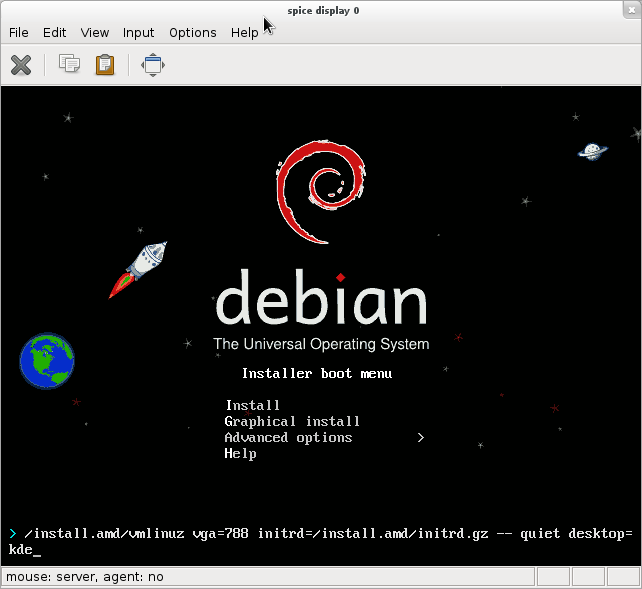
\includegraphics[width=7cm]{image201202/kdedesk/stable-inst-menu.png}
\caption{$B0BDjHG%$%s%9%H!<%k2hLL$G(BTAB$B%-!<$r2!$7$?$H$-$NMM;R(B}
\end{center}
\end{figure}
\item $B$"$H$ODL>o$I$*$j%$%s%9%H!<%k$r9T$$$^$9!#%$%s%9%H!<%k$r?J$a$F$$$/$H(B
$B!V%$%s%9%H!<%k$9$k%=%U%H%&%'%"$NA*Br(B:$B!W$N%a%K%e!<$,8=$l$^$9$N$G!"(B ``Debian desktop environment''
$B$rA*Br$7$F$*$$$F$/$@$5$$!#(B
\item $B%$%s%9%H!<%k$,40N;$7$^$7$?$i!"%j%V!<%H$r9T$$$^$9!#(B
\item KDE$B4D6-$,5/F0$7$^$9!#(B
\end{enumerate}

$B0J>e$H$J$j$^$9!#4JC1$G$9$M!#(B

\subsection{$B3+H/<T$H$7$F$N(Bexperimental$BHG(BKDE$BF3F~J}K!(B(KVM+spice)}
\label{sec:exp-kde}
\index{kvm}
\index{spice}

$BEl5~%(%j%"(BDebian$BJY6/2q$K$$$i$C$7$c$k$h$&$JJ}!9$K$O!"A0=R$N%$%s%9%H!<%k$H4D6-$G$O(B
$B$-$C$H!V$L$k%2!<!J>P!K!W$J46$8$N$O$:$G$9!#$=$N>l9g!"@'Hs$H$b(B
experimental$BHG$N(BKDE$B4D6-$rMxMQ$$$?$@$-!"(BBTS$B=q$-(B/$B%Q%C%A3+H/(B/$BK]Lu(B/$B%G%P%C%0$J$I$N(B
$B3+H/3hF0$K6P$7$s$G$_$^$7$g$&!#$3$3$G$O!"3+H/<T8~$1(BKDE$B4D6-F3F~$K$D$$$F4JC1$K=R$Y$^$9!#(B

\begin{itemize}
\item $B3+H/<T8~$1$K(Bexperimental$BHGF3F~$rA0Ds$K$7$^$9!#(B
\item $B2>A[4D6-$G$"$k(BKVM$B$rMxMQ$7$F2>A[4D6->e$KF3F~$7$^$9!#$3$l$J$i!"%G%#%9%/%$%a!<%8%U%!%$%k$r$H$C$F$*$1$P!"(B
$B$&$C$+$j(Bexperimental$B4D6-$G(Baptitude full-upgrade$B$7$FA4$/N)$A>e$,$i$J$/$J$C$F$b!J<BOC!K$"$C$5$jI|5"$G$-$^$9!#(B
\item $B%5%&%s%I$b$b$A$m$sM_$7$$$N$G2>A[%G%9%/%H%C%W4D6-$H$7$F(Bspice$B$r;H$$$^$9!#(B
\item $B$$$D$G$b$I$3$G$b3+H/$G$-$k$h$&$K%b%P%$%k4D6-$K9=C[$7$^$9!#(B
\end{itemize}
$B?^(B\ref{fig:kde-env}$B$N(BKDE$B3+H/4D6-$NMQ0U$rA[Dj$7$^$9!#(B

\begin{figure}[ht]
\begin{center}
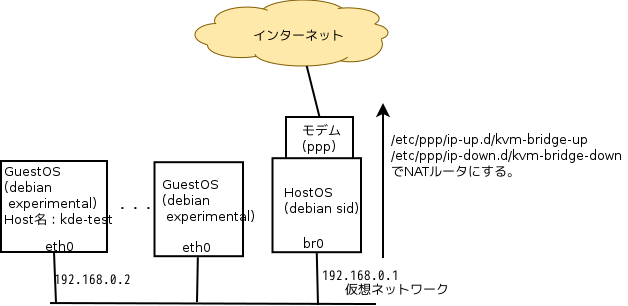
\includegraphics[width=10cm]{image201202/kdedesk/kde-dev-env.png}
\caption{\label{fig:kde-env}KDE$B3+H/4D6-(B}
\end{center}
\end{figure}

$B0J2<$OF3F~$K4X$7$F$NN.$l$G$9!#!J:Y$+$$;v$O3d0&$7$^$9!#A`:n$K$"$?$C$F$OE,59(Broot$B8"8B$,I,MW$@$C$?$j$7$^$9!K(B
\begin{enumerate}
\item HostOS$B$H$J$k(BPC$B$N(BBIOS$B$rA`:n$7$F!"(BCPU$B$N2>A[5;=Q;Y1g5!9=$N%9%$%C%A$r(BON$B$K$7$F%V!<%H$7$F$*$-$^$9!#(B
\item HostOS$B$K(B\url{http://www.debian.org/CD/netinst}$B$+$iL>;I%5%$%:$N(BCD$B%$%a!<%8$rMn$H$7$FCV$-$^$9!#(B
\item HostOS$B$N(B/etc/network/interfaces$B$K0J2<$NDI5-$r9T$$!"(Bbr0$B$r:n$C$F$*$-$^$9!#(B
\begin{commandline}
# $BDI5-$O$3$3$+$i!#(Baptitude install bridge-utils$B$O$d$C$F$*$/$3$H!#(B
auto br0
iface br0 inet static
        address 192.168.0.1
        netmask 255.255.255.0
        bridge_ports none
        bridge_stp off
        bridge_fd 0
        bridge_maxwait 0
\end{commandline}
\item HostOS$B$N(B/etc/sysctl.d/bridge-filter-workaround.conf$B$r:n$j!"(B\\
sysctl -p /etc/sysctl.d/bridge-filter-workaround.conf$B$r<B9T$7$F!"(Bbr0$B$N%U%#%k%?$rL58z2=$7$F$*$-$^$9!#(B
\begin{commandline}
# /etc/sysctl.d/bridge-filter-workaround.conf$B$NCf?H(B
net.bridge.bridge-nf-call-ip6tables = 0
net.bridge.bridge-nf-call-iptables = 0
net.bridge.bridge-nf-call-arptables = 0
\end{commandline}
\item HostOS$B$N(B/etc/ppp/ip-up.d/kvm-bridge-up,/etc/ppp/ip-down.d/kvm-bridge-down$B$r:n$C$F$*$-$^$9!#B>$K%U%#%k%?$H$+I,MW$G$"$l$PE,Ev$K$I$&$>!#(B
\begin{commandline}
#!/bin/sh
# /etc/ppp/ip-up.d/kvm-bridge-up$B$NCf?H(B
PATH=/bin:/usr/bin:/sbin:/usr/sbin
CDPATH=
sysctl -w net.ipv4.ip_forward=1
iptables -t nat -A POSTROUTING -o $PPP_IFACE -j MASQUERADE
iptables -A FORWARD -i br0 -o $PPP_IFACE -j ACCEPT
\end{commandline}
\begin{commandline}
#!/bin/sh
# /etc/ppp/ip-down.d/kvm-bridge-down$B$NCf?H(B
#!/bin/sh
PATH=/bin:/usr/bin:/sbin:/usr/sbin
CDPATH=
sysctl -w net.ipv4.ip_forward=0
iptables -t nat -D POSTROUTING -o $PPP_IFACE -j MASQUERADE
iptables -D FORWARD -i br0 -o $PPP_IFACE -j ACCEPT
\end{commandline}
\item HostOS$B$K(Bkvm/libvirt/spice-client-gtk$B%Q%C%1!<%8$rF3F~$7$F$*$-$^$9!#(B
\item HostOS$B$K$F(BGuestOS$BMQ$N(Bkde-test.xml$B$r0J2<$N?w7A$G:n@.$7$F(Bvirsh define kde-test.xml$B$7$F$*$-$^$9!#(B\footnote{virt-install$B$O2?8N$+<+J,$N(Bexperimental$B$J4D6-$G$O(BSegmentation Fault$B$GMn$A$F$7$^$&$N$G$3$3$G$O;H$$$^$;$s!#(BBTS$B$7$H$-$^$9!#(B}
\begin{commandline}
<domain type='kvm'>
  <name>kde-test</name>
  <memory>1048576</memory>
  <vcpu>1</vcpu>
  <os>
    <type arch='x86_64' machine='pc-1.0'>hvm</type>
    <boot dev='hd'/>
    <boot dev='cdrom'/>
    <bootmenu enable='yes'/>
  </os>
  <features>
    <acpi/>
    <apic/>
    <pae/>
  </features>
  <clock offset='utc'/>
  <on_poweroff>destroy</on_poweroff>
  <on_reboot>restart</on_reboot>
  <on_crash>restart</on_crash>
  <devices>
    <emulator>/usr/bin/kvm</emulator>
    <disk type='file' device='disk'>
      <driver name='qemu' type='raw' cache='writeback'/>
      <source file='/var/lib/libvirt/images/kde-test.img'/>
      <target dev='vda' bus='virtio'/>
    </disk>
    <disk type='file' device='cdrom'>
      <driver name='qemu' type='raw'/>
<!-- directory of cdimage$B$OE,Ev$KJQ99$/$@$5$$(B -->
      <source file='/directory of cdimage/debian-6.0.4-amd64-businesscard.iso'/>
      <target dev='hdc' bus='ide'/>
      <readonly/>
    </disk>
    <controller type='ide' index='0'/>
    <interface type='bridge'>
<!-- mac$B%"%I%l%9$OE,Ev$KJQ99$/$@$5$$(B -->
      <mac address='52:54:00:31:cd:5a'/>
      <source bridge='br0'/>
      <model type='virtio'/>
    </interface>
    <serial type='pty'>
      <target port='0'/>
    </serial>
    <console type='pty'>
      <target type='serial' port='0'/>
    </console>
    <input type='mouse' bus='ps2'/>
    <graphics type='spice' port='5900' autoport='no'>
      <clipboard copypaste='yes'/>
    </graphics>
    <sound model='ac97'\>
    <video>
      <model type='qxl' vram='9216' heads='1'/>
    </video>
    <memballoon model='virtio'>
    </memballoon>
  </devices>
</domain>
\end{commandline}
\item HostOS$B$G2>A[4D6-MQ$N%G%#%9%/$r(B10GB$B$0$i$$$G:n$C$F$*$-$^$9!#(B
\begin{commandline}
qemu-img create -f raw /var/lib/libvirt/images/kde-test.img 10G
\end{commandline}
\item HostOS$B$G(BKVM$B$r5/F0$7$F!"(Bspice$B%/%i%$%"%s%H$r@\B3$7$^$9!#(B
\begin{commandline}
virsh start kde-test; spicy -h 127.0.0.1 -p 5900 &
\end{commandline}
\item GuestOS$B$N(BDebian$B%$%s%9%H!<%i$,5/F0$7$?$i!"(BTAB$B%-!<$r2!$7!"2hLL2<$K8=$l$?JT=82DG=$J9T$K!"(B''priority=medium''$B$r0J2<$N$h$&$KF~NO$7$F%$%s%9%H!<%k$r3+;O$7$^$9!#(B
\begin{commandline}
 /install.amd/vmlinuz vga=788 initrd=/install.amd/initrd.gz --- quiet priority=medium
\end{commandline}
$B%$%s%9%H!<%kESCf!V(BDebian $B%"!<%+%$%V$N%_%i!<$rA*Br!W$N%a%K%e!<$K$F(B''sid''$B$rA*Br$7!"!V%$%s%9%H!<%k$9$k%3%s%]!<%M%s%H!W$H$7$F!V(Bssh$B%5!<%P!<!W$N$_(B($BB>$OA*Br$7$J$$(B)$B$H$7$^$9!#(B
\item $B%$%s%9%H!<%k$,40N;$9$k$H!"%F%-%9%H%3%s%=!<%k$+$i(BDebian sid$B$J(BGuestOS$B$X%m%0%$%s$G$-$k$h$&$K$J$j$^$9!#(B
\item GuestOS$B$K%m%0%$%s$7$F0J2<$N9T$r(B/etc/apt/source.list$B$XIU$12C$($^$9(B
\begin{commandline}
#$BDI2CFbMF(B
deb http://ftp.jp.debian.org/debian/ experimental main
deb-src http://ftp.jp.debian.org/debian/ experimental main
\end{commandline}
\item GuestOS$B$N(B/etc/apt/preference.d$B$K(BDebian KDE$B%A!<%`@=$N(Bexperimental$B%Q%C%1!<%8MQ(Bpreference$B%U%!%$%k$r%$%s%9%H!<%k$7$^$9!#(B
\begin{commandline}
cd /etc/apt/preference.d && wget http://pkg-kde.alioth.debian.org/files/kde-experimental
\end{commandline}
\item GuestOS$B$G0J2<$r<B9T$7!"(Bexperimental$B$J(BKDE$B4D6-$r0l5$$KF~$l$F$7$^$$$^$9!#(B
\begin{commandline}
aptitude update;aptitude aptitude install task-kde-desktop task-japanese-kde-desktop;aptitude clean
\end{commandline}
\item $B%$%s%9%H!<%k$,=*$o$C$?$i!"(BGuestOS$B$r%j%V!<%H$7$^$9!#(BGuestOS$B$G(BKDE$B$N(Bexperimental$BHG$,5/F0$7!"%0%i%U%#%+%k$J%m%0%$%s2hLL$,8=$l$^$9!#(B
\end{enumerate}

\subsection{Debian$B$H(BKDE$B4D6-$N%P!<%8%g%s(B}

Debian$B$N%P!<%8%g%s$H(BKDE$B$N%P!<%8%g%s$NBP1~$rI=(B\ref{tab:kde-ver}$B$K:\$;$^$9!#(B

\begin{table}[ht]
\begin{center}
\begin{tabular}{|l|l|l|l|l||l|}
\hline
Debian&stable&testing&unstable&experimental&upstream\\
\hline \hline
KDE &4.4&4.6&4.6&4.7.4&4.8.0\\
\hline
\end{tabular}
\caption{\label{tab:kde-ver}Debian$B$N%P!<%8%g%s$H(BKDE$B$N%P!<%8%g%s(B}
\end{center}
\end{table}

KDE$B$N(Bupstream$B$O(B2012$BG/(B1$B7n(B25$BF|$K(B4.8.0$B$r%j%j!<%9$7$?$P$+$j$J$N$G!"$^$@(B
experimental$B$bDI$$$D$$$F$$$J$$>uBV$G$9!#(B

\subsection{KDE$B4D6-$N3+H/$NFCD'(B}

KDE$B4D6-$N3+H/$O0J2<$N$h$&$JFCD'$,$"$j$^$9!#(B

\begin{enumerate}
\item Qt$B!J%-%e!<%H!K%i%$%V%i%j$r;H$&!#(B
\item C++$B$N%3!<%I$,4pK\(B
\item autotools$B$NBe$o$j$K(Bcmake$B$,;H$o$l$k(B
\end{enumerate}

$B$3$N$?$a!"(BDebian$B$G$O%Q%C%1!<%83+H/$N0Y$K(Bpkg-kde-tools$B%Q%C%1!<%8$,MQ0U$5$l$F$$$^$9!#(B

\subsection{Debian$B$G$N(BKDE$B4D6-$N%Q%C%1!<%83+H/(B}

Debian$B$G$O(BKDE$B4D6-$N%Q%C%1!<%83+H/MQ$K(Bpkg-kde-tools$B$H$$$&%Q%C%1!<%8$rJL$KMQ0U$7$F$$$^$9!#$3$A$i$rF3F~$9$k$H(BKDE$B4D6-$N%Q%C%1!<%89=C[$N:]$KJXMx$J5!G=$,;H$($k$h$&$K$J$j$^$9!#(B

\begin{table}[ht]
\begin{center}
\begin{tabular}{|l|l|l|l|}
\hline
$B9`HV(B&$B3HD%$5$l$k$b$N(B&$B3HD%(B&$BHw9M(B\\
\hline
1&dh& --with kde & debhelper$B$K(Bkde$BMQ$N3HD%$r;XDj(B\\
\hline
2&dh\_auto\_*& --buildsystem=kde & dh\_auto\_*$B$,(Bcmake$B$r;H$&$h$&$K$J$k!"(BKDE$B4D6-MQ$N@_Dj$r9T$&Ey(B\\
\hline
3&CDBS&kde.mk& CDBS$B$G(BKDE$BMQ$N3HD%$,MxMQ$G$-$k$h$&$K$J$k(B\\
\hline
4&$B$=$NB>(B&variables.mk$B$J$I(B& debian/rules$B$NCf$G(B\$(DEB\_CMAKE\_KDE4\_FLAGS)$B$J$I$,;H$($kEy(B\\
\hline
\end{tabular}
\caption{\label{tab:pkg-kde-tools-inst}pkg-kde-tools$B$r%$%s%9%H!<%k$7$?;~$N3HD%(B}
\end{center}
\end{table}

\subsection{$BD64J0WE*$K(BKDE$BMQ%W%m%0%i%`$N(BDebian$B%Q%C%1!<%8$r:n$C$F$_$k(B}

$B$3$3$G$OD64J0WE*$K(BKDE$BMQ%W%m%0%i%`$N(BDebian$B%Q%C%1!<%8$r:n$C$F$_$^$9!#(B
$B$^$:!";vA0=`Hw$H$7$F!"(B

\begin{itemize}
\item$B!!4D6-$O(B\ref{sec:exp-kde}$B>O$N(Bexperimental$B4D6-$rMQ0U$/$@$5$$!#(B
\item  $BI,MW$J%Q%C%1!<%8(B(cmake$B%Q%C%1!<%8Ey(B)
\footnote{KDE$B4D6-8~$1$N3+H/$,A4$/=i$a$F$N?M$O!":Y$+$$;v$,H=$C$F$/$k$^$G!"(Baptitude build-dep kdeutils$B$7$F$*$$$F(BKDE$B%Q%C%1!<%83+H/$KI,MW$J%Q%C%1!<%8$r$"$i$+$8$a$^$H$a$FF3F~$7$F$*$/$H$$$&<j$b$"$j$^$9(B}
\end{itemize}

$B<!$K(Bkhello-1.0.0/$B$J$k%G%#%l%/%H%j$K(B\url{http://techbase.kde.org/Development/Tutorials/First_program}$B$K$"$k!"(Bmain.cpp$B$H(BCMakeLists.txt$B$rG[CV$7$^$9!#(B

\begin{commandline}
$ cd khello-1.0.0
$ ls
CMakeLists.txt main.cpp
$
\end{commandline}
% $

$B<!$K!"%*%j%8%J%k$N(Btar.gz$B%"!<%+%$%V$r:n@.$7$F$*$-$^$9!#(B

\begin{commandline}
$ cd ..
$ tar czf khello_1.0.0.orig.tar.gz khello-1.0.0
$ ls -F
khello-1.0.0/  khello_1.0.0.orig.tar.gz
$
\end{commandline}

dh\_make $B$r;H$C$F(Bdebian/$B%G%#%l%/%H%j$r;E9~$_$^$9!#$"$H$O(Brules$B%U%!%$%k0J30(B
$B$$$D$bDL$j!"%Q%C%1!<%8$r:n@.$9$k$h$&$K%U%!%$%k$r:n@.$7$F$*$-$^$9!#(B

\begin{commandline}
$ cd khello-1.0.0/debian
$ ls -F
README.Debian  changelog  control    docs   source/
README.source  compat     copyright  rules
$
\end{commandline}
% $

pkg-kde-tools$B%Q%C%1!<%8$rMxMQ$9$k(Brules$B%U%!%$%k$r5-:\$7$^$9!#(B

\begin{commandline}
# pkg-kde-tools$B$r;H$C$?(BKDE$B3+H/MQ(Bdebian/rules$B%U%!%$%k$NCf?H!#(B

%:
       dh $@ --with kde
\end{commandline}
%$

$B$"$H$O!"(Bdpkg-buildpackage -uc -us -rfakeroot$B$r<B9T$7$F%S%k%I$7$^$9!#(B

\begin{commandline}
$ dpkg-buildpackage -us -uc -rfakeroot
dpkg-buildpackage: source package khello
...$BCfN,(B...
dpkg-source: info: building khello in khello_1.0.0-1.debian.tar.gz
dpkg-source: info: building khello in khello_1.0.0-1.dsc
 debian/rules build
dh build  --with kde
   dh_testdir
   dh_auto_configure --buildsystem=kde
-- The C compiler identification is GNU
-- The CXX compiler identification is GNU
...$BCfN,(B...
\end{commandline}
%$

$BL5;v!"(B--buildsystem=kde$B$,MxMQ$5$l!"(Bcmake$B$,<B9T$5$l$F$$$^$9!#(B

$B$7$P$i$/BT$D$HL5;v$K(Bkhello\_1.0.0-1\_amd64.deb$B$J$I$,=PMh>e$,$j$^$9!#(B

$B$[$i!"(Bpkg-kde-tools$B$N$*$+$2$G%Q%C%1!<%83+H/$b4JC1$G$7$g(B?$B$G$7$g!)(B

\subsection{$B$*$o$j$K(B}

$B:#2s$O!"(BDebian$B3+H/<T$N0Y$N(BKDE$B4D6-$N9=C[$H!"4JC1$J%Q%C%1!<%8:n@.$K$D$$$F!"(B
$B0lDL$j5-:\$7$F$_$^$7$?!#$3$l$r5!$K!"(BKDE$B4D6-$K4X$9$k3+H/$r$5$l$kJ}$,A}$($k$H(B
$B$&$l$7$$$H;W$C$F$$$^$9!#(B

\subsection{$B;29MJ88%(B}

\begin{itemize}
\item \url{http://pkg-kde.alioth.debian.org/} Debian KDE Team$B$N%[!<%`%Z!<%8!#(B
\item \url{http://techbase.kde.org} KDE Techbase
\item \url{http://kde.org/} KDE$BK\2H(B
\item \url{http://www.spice-space.org/} SPICE$B2>A[%G%9%/%H%C%W%G%P%$%9K\2H(B
\end{itemize}

\clearpage
%-------------------------------------------------------------------------------
\dancersection{CMake$B$r;H$C$F$_$k(B}{$BLnEg(B $B5.1Q(B}
%-------------------------------------------------------------------------------
\index{cmake}

\subsection{CMake$B$H$O(B}

KDE$B4D6-$N3+H/$K;H$o$l$F$$$k%D!<%k$K(BCMake$B$,$"$j$^$9!#$3$l$O=>Mh$N(Bautotools
$B$N$h$&$J$b$N$G$9!#$,!"(Bautotools$B$KHf$Y$F<!$K=R$Y$kBeI=E*$JFCD'$,$"$j$^$9!#(B

\begin{itemize}
\item $B%P%$%J%j$N%W%m%0%i%`$G$"$k(B\\
autotools$B$O!"$4B8CN$NDL$j!"Cf$O(Bsh$B%9%/%j%W%H$H$J$C$F$$$^$9!#$3$l$O(B
/bin/sh$B$r4pK\%3%^%s%I$H$7$F;}$D=>Mh$N(BUNIX$B7O$N(BOS$B$G;H$&$J$iHs>o$KET9g$,$h(B
$B$$$N$G$9$,!"$=$b$=$b(B/bin/sh$B$r;}$?$J$$%7%9%F%`$N85$GMxMQ$7$h$&$H$9$k$H(B
$BF0:n$G$-$^$;$s!#$3$l$G$O!"Nc$($P!"I8=`E*$J(BC$B%W%m%0%i%`$r%3%s%Q%$%k=PMh$k4D6-(B
$B$J$N$K!"(B/bin/sh$B$,L5$$$H$$$&K\<A$G$O$J$$M}M3$N0Y$K0\?"@-$rB;$J$&$N$O$A$g$C$H(B
$B;DG0$G$9!#(B

CMake$B$O%P%$%J%j$N%W%m%0%i%`$J$N$G!"%3%^%s%IC1BN$GF0:n$9$k$3$H$,$G$-!"(B
/bin/sh$B$J$I(BUNIX$B$N%3%^%s%I$,L5$$>l=j$G$bLdBj$J$/F0:n$G$-$^$9!#(B

\item $BMM!9$J%W%i%C%H%U%)!<%`MQ$N9=C[%7%9%F%`$KBP1~$G$-$k(B\\
$B!!(Bautotools$B$O(Bmake$B$KFC2=$7$?%D!<%k$H$J$j$^$9!#$3$3$G!"$=$b$=$b(BMakefile$B$,(B
$B0lHLE*$G$O$J$$3+H/4D6-!JNc!'(BMicrosoft Visual Studio$BEy$NMM!9$J(BIDE)$B$N>l9g!"(B
Makefile$B$h$j$b(BIDE$B$N%W%m%8%'%/%H%U%!%$%k$r@8@.$G$-$?J}$,$h$jET9g$,$h$+$C$?$j$7$^$9!#(B
CMake$B$O0lK\$N(BCMakeLists.txt$B$rMQ0U$9$k$@$1$G!"(BMakefile$B$d!"(BIDE$B4D6-MQ(B
$B$N%W%m%8%'%/%H%U%!%$%k$r@8@.$G$-$?$j$9$kG=NO$,$"$j$^$9!#$3$N0Y!"(Bautotools$B$r(B
$BMxMQ$7$?%=!<%9%Q%C%1!<%8$N$h$&$K!"(BMakefile.am$B$H!"Nc$($P(B.vcproj$B%U%!%$%k$rJL!9$K(B
$B=$@5$7$F(BUNIX/Windows$B4V$N0\?"@-$rJ]$D$H$$$&$h$&$J:n6H$+$i3+H/<T$,3+J|(B
$B$5$l$k2DG=@-$r0UL#$7$^$9!#(B

\item $B$=$NB>(B\\
 $B>\$7$$%5%^%j$O!"(BDDJ$B%8%c!<%J%k$N(B\url{http://drdobbs.com/cpp/184405251}$B$K(B
$B%5%^%j$5$l$F$$$k$h$&$J5!G=$,$"$kLOMM$G$9!J$^$@<+J,$OL$I>2A$G$9!#!K(B

$B$3$N5-;v$+$i$$$/$D$+H4?h$9$k$H!"(B

\begin{itemize}
\item QT$B%i%$%V%i%j$N(Bmoc$B%3%^%s%I(B/ITK$B$N(BCABLE/VTK$B$N%i%C%Q!<@8@.%3%^%s%I$KBP1~$7$?%9%F!<%H%a%s%H(B
\item $B@EE*%i%$%V%i%j!"F0E*%i%$%V%i%j$N@8@.$rMF0W$K@Z$jBX$($l$k$h$&$K$9$k5!G=(B
\item $B%U%!%$%k$N0MB84X78$N<+F0@8@.!"JBNs%S%k%I$N%5%]!<%H(B
\end{itemize}

$B$,$"$kLOMM$G$9!#(B
\end{itemize}

\subsection{$B;H$C$F$_$k(B}

$BI4J9$O0l8+$K$7$+$:$J$N$G!"$A$g$C$H;H$C$F$_$^$9!#(B

cmake$B%Q%C%1!<%8$r%7%9%F%`$KF3F~$7$^$9!#(B

\begin{commandline}
$ sudo aptitude install cmake
\end{commandline}
%$

$B<!$K0J2<$N%=!<%9(B(hello.c,config.h.in)$B$rMQ0U$7$^$9!#(B

\begin{commandline}
/*hello.c*/
#include <stdio.h>
#include "config.h"
int main(int argc,char **argv)
{
	printf("hello world\n");
#if defined(HAVE_EXIT)
	printf("yes, this system has exit()\n");
#endif
	return(0);
}
\end{commandline}
\begin{commandline}
/*config.h.in*/
#cmakedefine HAVE_EXIT
\end{commandline}

$B<!$K!"(BCMakeLists.txt$B$rMQ0U$7$^$9!#(B
\begin{commandline}
# cmake$B$N%P!<%8%g%s$O(B2.8$B0J>e(B
cmake_minimum_required(VERSION 2.8)
# project$B$NL>A0$r@k8@(B
project(hello)

# CMake$BDs6!$N%^%/%m$r%m!<%I$9$k!#$3$3$G$O4X?t$,%7%9%F%`$K$"$k$+$r3N$+$a$k%^%/%m(B
# $B$r;H$C$F$_$k!#(B
include (${CMAKE_ROOT}/Modules/CheckFunctionExists.cmake)

# exit()$B4X?t$r%A%'%C%/$7$F$_$k!#$"$l$P(BHAVE_EXIT$B$rDj5A$;$h$H$$$&0UL#!#(B
check_function_exists(exit HAVE_EXIT)

configure_file (
  "${PROJECT_SOURCE_DIR}/config.h.in"
  "${PROJECT_BINARY_DIR}/config.h"
)
# cc -I$B$K2?;XDj$9$k$+(B
include_directories ("${PROJECT_BINARY_DIR}")

# hello$B$O(Bhello.c$B$+$i=PMh$k$H$$$&;v$r;XDj(B
add_executable(hello hello.c)
\end{commandline}

$B$3$l$i(B3$B$D$N%U%!%$%k$r(Bhello-src/$B0J2<$KG[CV$7$^$9!#(B
\begin{commandline}
$ ls -lR
.:
$B9g7W(B 4
drwxr-xr-x 2 nojima nojima 4096  2$B7n(B 17 03:15 hello-src

./hello-src:
$B9g7W(B 8
-rw-r--r-- 1 nojima nojima 46  2$B7n(B 17 03:15 CMakeLists.txt
-rw-r--r-- 1 nojima nojima  34  2$B7n(B 17 04:21 config.h.in
-rw-r--r-- 1 nojima nojima 91  2$B7n(B 17 03:10 hello.c
$
\end{commandline}

$B:#2s$O%S%k%IMQ%G%#%l%/%H%j(B(hello-build)$B$r:n$j!"0\F0$7$^$9!#(B

\begin{commandline}
$ ls
hello-src
$ mkdir hello-build
$ cd hello-build
\end{commandline}
% $

cmake$B$r<B9T$7$^$9!#(B

\begin{commandline}
$ cmake ../hello-src
-- The C compiler identification is GNU
-- The CXX compiler identification is GNU
-- Check for working C compiler: /usr/bin/gcc
-- Check for working C compiler: /usr/bin/gcc -- works
...$BCfN,(B...
-- Looking for exit
-- Looking for exit - found
-- Configuring done
-- Generating done
-- Build files have been written to: /.../cmake-test/hello-build
$ ls
CMakeCache.txt  CMakeFiles  Makefile  cmake_install.cmake  config.h
\end{commandline}

$B<+F0E*$K4D6-%A%'%C%/$,9T$o$l(BMakefile/config.h$B$,=PMh>e$,$j$^$9!#(B
exit$B4X?t$b8+$D$+$C$?$H$NI=<($,9T$o$l$^$7$?!#$3$3$G(Bmake$B$7$F$_$^$9!#(B

\begin{commandline}
$ make
Scanning dependencies of target hello
[100%] Building C object CMakeFiles/hello.dir/hello.c.o
Linking C executable hello
[100%] Built target hello
$ ls -F
CMakeCache.txt  CMakeFiles/  Makefile  cmake_install.cmake  config.h  hello*
$ ./hello
hello world
yes, this system has exit()
$
\end{commandline}

CMakeLists.txt$B$+$iL5;v$K<B9T%P%$%J%j(B(hello)$B$,=PMh>e$,$j$^$7$?!#$^$?!"(Bdefined(HAVE\_EXIT)$B$b(BTrue$B$H$J$j!"(Bexit()$B4X?t$,$"$k;~$N%3!<%I$b%3%s%Q%$%k$5$l$F$$$^$9!#(B

\subsection{IDE$BMQ$N%W%m%8%'%/%H%U%!%$%k$r@8@.$7$F$_$k(B}

cmake$B$r0z?tL5$7$G<B9T$9$k$H!"(Bhelp$B$,=P$F$-$^$9!#$3$N%X%k%W$NJ8>O$NCf$K!"$I$s$J(BIDE$BMQ$N%W%m%8%'%/%H%U%!%$%k$r@8@.$G$-$k$+$K$D$$$F@bL@$,$"$j$^$9!#;n$7$K<j85$N(BDebian$B%^%7%s$G<B9T$9$k$H!"(B

\begin{commandline}
$ cmake
...$BCfN,(B..
The following generators are available on this platform:
  Unix Makefiles              = Generates standard UNIX makefiles.
  CodeBlocks - Unix Makefiles = Generates CodeBlocks project files.
  Eclipse CDT4 - Unix Makefiles
                              = Generates Eclipse CDT 4.0 project files.
  KDevelop3                   = Generates KDevelop 3 project files.
  KDevelop3 - Unix Makefiles  = Generates KDevelop 3 project files.
$
\end{commandline}

$B$3$3$G$O;n$7$K@h$[$I$N(Bhello-build$B%G%#%l%/%H%j0J2<$G(BKDevelp3 project $B%U%!%$%k$r@8@.$7$F$_$^$9!#(B

\begin{commandline}
$ cmake -G KDevelop3 ../hello-src
...$BCfN,(B...
$ ls
MakeCache.txt  Makefile             config.h        hello.kdevelop.filelist
CMakeFiles     cmake_install.cmake  hello.kdevelop  hello.kdevses
$
\end{commandline}
%$
$B3N$+$K(BKDevelp3$BMQ$N%W%m%8%'%/%H%U%!%$%k(B(hello.kdevelop$BEy(B)$B$,@8@.$5$l$F$$$^$9!#(B

\subsection{$B$*$o$j$K(B}

cmake$B$O(BKDE$B$NB>$K$b(Bmysql$B$G$b:NMQ$5$l$F$$$^$9!#$^$?!"(Bwikipedia(\url{http://ja.wikipedia.org/wiki/CMake})$B$K$h$l$P!"MxMQ$7$F$$$k%"%W%j%1!<%7%g%s$bB3!9A}$($F$$$kLOMM$G$9!#(B

$B;H$$$3$J$;$k$H6/NO$J%D!<%k$H$J$j$=$&$J46$8$G$9!#3'$5$s$b;H$C$F$_$F$O$$$+$,$G$7$g$&$+!)(BDebian$B$J$i(Baptitude$B$G4JC1$KF3F~$G$-$^$9$N$G!"@'Hs;n$7$F$_$F$/$@$5$$!#(B

\subsection{$B;29MJ88%(B}

\begin{itemize}
\item \url{http://www.cmake.org/} CMake$BK\2H(B
\item \url{http://www.cmake.org/cmake/help/cmake_tutorial.html} CMake$B%A%e!<%H%j%"%k(B
\item \url{http://drdobbs.com/cpp/184405251?pgno=1} DDJ$B%8%c!<%J%k$N5-;v(B
\end{itemize}


%-------------------------------------------------------------------------------
\dancersection{Apache2 / HTTP $B%5!<%P$+$i;O$a$k(B Debian}{$B4d>>(B $B?.MN(B}
%-------------------------------------------------------------------------------
\index{apache}

$BIaCJ$O$A$g$C$H3+H/<T4s$j$JOC$r$7$F$$$k(BDebian
$BJY6/2q$G$9$,!":#2s$O(B OSC $B=PD%4k2h$H$7$F!"%f!<%6!<;kE@$NJY6/2q$r3+:E$7$^$9!#(B
$B:#2s$O$h$/;H$o$l$F$$$k$H;W$o$l$k(B Apache2 / HTTP $B%5!<%P(B $B$K>GE@$rEv$F$F$_$^$9!#(B

\subsection{$B$O$8$a$K(B}

Debian $B$O(B $BF|K\$G$O(B HTTP $B%5!<%P$H$7$FMxMQ$5$l$F$$$k$h$&$K8+$($^$;$s$,!"(B
$B@$3&$G$O0lHV:NMQ$5$l$F$$$k(B Linux $B%G%#%9%H%j%S%e!<%7%g%s$K$J$C$?$h$&$G$9!#(B
\footnote{\url{http://w3techs.com/blog/entry/debian_is_now_the_most_popular_linux_distribution_on_web_servers}}
$B$3$N5-;v$K$h$k$H!"MxMQ$5$l$F$$$kM}M3$O(B HTTP $B%5!<%P%Q%C%1!<%8$N<oN`$,B?$/$"$k;v$,M}M3$N0l$D$K5s$2$i$l$F$$$^$9!#(B
Debian $B$r(B HTTP $B%5!<%P$H$7$FMxMQ$7$F$$$kM}M3$r<B:]$K;H$C$F$$$kJ}$KJ9$$$F$_$?$H$3$m!"M}M3$O$3$l$@$1$G$O$J$$$3$H$,J,$+$j$^$7$?!#(B
Debian$B$N%Q%C%1!<%8%s%0%7%9%F%`!"(BAPT$B!"(BApahce $B%b%8%e!<%k%Q%C%1!<%8$NB?$5!"(B
Web$B%"%W%j%1!<%7%g%s$G:NMQ$5$l$k(B P$B8@8l!J(BPerl, Python, PHP$B!K$N%5%]!<%H$J$I$,$"$j!"(B
$B0lHVNI$$E@$H$7$F5s$2$i$l$?$N$O@_Dj%U%!%$%k$N=@Fp@-$K$D$$$F$G$7$?!#(B

Debian $B$N(B Apache2 / HTTP $B%5!<%P(B $B$O(B Red Hat $B7O(B $B$H0c$$!"(BDebian $BFCM-$N9=@.$K$J$C$F$$$^$9!#$3$l$OB>$N%G%#%9%H%j%S%e!<%7%g%s$7$+(B
$BCN$i$J$$?M$K$H$C$F$OFq$7$$$+$b$7$l$^$;$s!#(B
$B$7$+$7(BDebian$BFCM-$N9=@.$rM}2r$9$k$H!"B>$N%G%#%9%H%j%S%e!<%7%g%s$H$N%a%j%C%H!"(B
$B%G%a%j%C%H$,8+$($F$/$k$H;W$$$^$9!#(B
$B$H$$$&$o$1$G:#2s$O!"(BDebian $B$N(B Apache2 / HTTP $B%5!<%P(B ($B0J2<!"(BApache2 $B!K(B $B$K$D$$$FJY6/$7$F$$$-$^$7$g$&!#(B

\subsection{Debian $B$N(B Apache2 $B%P!<%8%g%s(B}

$B$^$:!"(BDebian $B$GDs6!$5$l$F$$$k(B Apache2 $B$N%P!<%8%g%s$r8+$F$_$^$9!#(B
$BI=(B\ref{tab:apache-version}$B$K$^$H$a$^$7$?!#(B
Upstream $B$HHf$Y$k$H>/$78E$$$G$9$,!"5!G=E*$K$OLdBj$J$$$G$7$g$&!#(B
RHEL$B!"(BCentOS$B!J(B\texttt{$B%P!<%8%g%s(B 2.2.15-15}$B!K(B
$B$HHf$Y$F$bFC$K%P!<%8%g%s$,8E$$$H$$$&$o$1$G$b$"$j$^$;$s!#(B

\begin{table}[ht]
\begin{center}
\begin{tabular}{|l|l|l|l|l|l|}
\hline
$B%G%#%9%H%j%S%e!<%7%g%s(B & stable & testing &unstable & experimental & upstream\\
\hline \hline
$B%P!<%8%g%s(B & 2.2.16-6+squeeze6 & 2.2.22-1 & 2.2.22-1 & - & 2.4.1 \\
\hline
\end{tabular}
\caption{\label{tab:apache-version}Debian $B%G%#%9%H%j%S%e!<%7%g%s$H(B Apache2 $B$N%P!<%8%g%s(B}
\end{center}
\end{table}

\subsection{Debian$B$N%Q%C%1!<%89=@.$H%Q%C%1!<%8$N%$%s%9%H!<%k(B}

$B<!$K(B Apache2 $B$N%Q%C%1!<%89=@.$H%$%s%9%H!<%kJ}K!$K$D$$$F@bL@$7$^$9!#(B

\subsubsection{$B%Q%C%1!<%89=@.(B}

Debian $B$N(B Apache2 $B$GDs6!$5$l$F$$$k%Q%C%1!<%8$O0J2<$NDL$j$G$9!#(B
HTTP $B%5!<%P$N=hM}%b%G%k$4$H$K%Q%C%1!<%8(B
$B!J(Bapache2-mpm-worker$B!"(Bapache2-mpm-prefork$B!"(Bapache2-mpm-event$B!"(Bapache2-mpm-itk$B!K(B
$B$,J,N%$5$l$F$$$k$3$H$,$o$+$j$^$9!#(B
$B$3$l$K$h$j<+J,$NMQES$K9g$o$;$?%Q%C%1!<%8$r%$%s%9%H!<%k$G$-$^$9!#(B
Red Hat$B7O$O0l$D$N%Q%C%1!<%8$KE;$^$C$F$$$F!"=hM}%b%G%kKh$K%5%U%#%C%/%9$r$D$1$F$$$^$9!JNc!'(Bhttpd.worker$B!K!#(B
\begin{table}[ht]
\begin{center}
\begin{tabular}{|l|l|}
\hline
$B%Q%C%1!<%8L>(B & $B%Q%C%1!<%8$N@bL@(B\\
\hline \hline
apache2 & Apache HTTP $B%5!<%P%a%?%Q%C%1!<%8(B \\
\hline
apache2-mpm-worker & $B%9%l%C%I%b%G%k(B Apche HTTP $B%5!<%P(B\\
\hline
apache2-mpm-prefork & $BHs%9%l%C%I%b%G%k(B Apache HTTP $B%5!<%P(B\\
\hline
apache2-mpm-event & $B%$%Y%s%H%I%j%V%s%b%G%k(B Apache HTTP $B%5!<%P(B\\
\hline
apache2-mpm-itk & $B%^%k%A%f!<%64D6-(B  Apache HTTP $B%5!<%P(B\\
\hline
apache2.2-common & Apache HTTP $B%5!<%P(B $B6&DL%U%!%$%k(B \\
\hline
apache2.2-bin & Apache HTTP $B%5!<%P$N6&DL%P%$%J%j%U%!%$%k(B\\
\hline
apache2-utils & $B%&%'%V%5!<%PMQ%f!<%F%#%j%F%#%W%m%0%i%`(B \\
\hline
apache2-suexec & Apache2 mod-suexec $BMQ(B $B4pK\(B suexec $B%W%m%0%i%`(B \\
\hline
apache2-suexec-custom & Apache2 mod-suexec $BMQ(B $B@_Dj2DG=(B suexec $B%W%m%0%i%`(B \\
\hline
apache2-dbg & Apache HTTP $B%5!<%P(B $B%G%P%C%0%7%s%\%k%U%!%$%k(B \\
\hline
apache2-prefork-dev & $BHs%9%l%C%I%b%G%k(B Apache HTTP $B%5!<%P(B $B3+H/MQ%X%C%@%U%!%$%k(B\\
\hline
apache2-threaded-dev & $B%^%k%A%9%l%C%I%b%G%k!!(BApache HTTP $B%5!<%P(B $B3+H/MQ%X%C%@%U%!%$%k(B \\
\hline
apache2-doc & Apache HTTP $B%5!<%P%I%-%e%a%s%H(B \\
\hline
\end{tabular}
\caption{\label{tab:apache-pkg}Debian $B$G(B $BDs6!$5$l$k(B Apache2 $B%Q%C%1!<%8(B}
\end{center}
\end{table}

$B<!$K%Q%C%1!<%8$N0MB84X78?^$r?^(B\ref{fig:apache-pkg-dep}$B$K<($7$^$9!#0MB84X78$,J#;($J$N$G(B
$B%f!<%6$OIT0B$K$J$k$+$b$7$l$^$;$s!#$7$+$7(BDebian$B$G$O(B
$B6/NO$J%Q%C%1!<%84IM}%D!<%k(B APT $B$K$h$C$F5$$K$9$k;v$J$/%$%s%9%H!<%k$G$-$^$9!#(B

\begin{figure}[ht]
 \begin{center}
  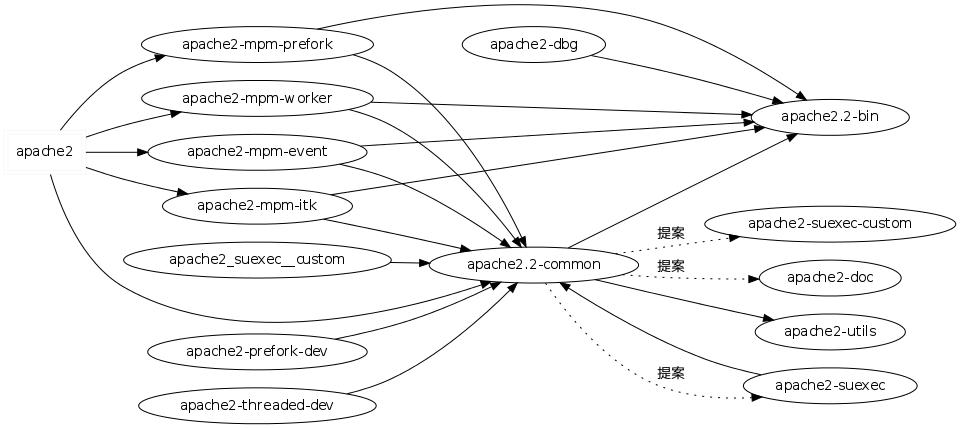
\includegraphics[width=1.0\hsize]{image201203/apache2-pkg.png}
 \end{center}
\label{fig:apache-pkg-dep}\caption{Debian $B$G$N%Q%C%1!<%80MB84X78(B}
\end{figure}

\subsubsection{$B%$%s%9%H!<%k(B}

Debian$B$G(B Apache2 $B$r%$%s%9%H!<%k$9$k>l9g$O(B \texttt{apt-get install}$B%3%^%s%I$r(B
$B;H$$$^$9!J?^(B\ref{fig:install}$B!K!#(B

Debian$B$G$O(B apache2 $B$H$$$&%a%?%Q%C%1!<%8$r;H$C$F%$%s%9%H!<%k$9$k$3$H$,B?$$$G$9!#(B
apache2 $B$r%$%s%9%H!<%k$9$k$H!"(Bapache2-mpm-worker $B$,%$%s%9%H!<%k$5$l$^$9!#(B
$BB>$N(B HTTP $B%5!<%P%Q%C%1!<%8$r%$%s%9%H!<%k$7$?$$>l9g$O!"3F!9$N%Q%C%1!<%8$r(B
$B;XDj$7$F%$%s%9%H!<%k$9$kI,MW$,$"$j$^$9!#(B

$B$^$?(BCentOS$B$J$I$G$O!"!V(Bhttpd$B!W(B $B%Q%C%1!<%8$H$7$FDs6!$5$l$F$$$k$N$G%Q%C%1!<%8L>$,0[$J$j$^$9!#(B
$BIaCJ$OB>$N%G%#%9%H%j%S%e!<%7%g%s$r;H$C$F$$$k?M$OCm0U$7$^$7$g$&!#(B


\begin{figure}[ht]
 \begin{center}

\begin{commandline}
$ sudo apt-get update          // $B%j%]%8%H%j$r99?7(B
$ sudo apt-get install apache2 // apache2 $B%Q%C%1!<%8$r%$%s%9%H!<%k(B
\end{commandline}
%$

 \end{center}
\label{fig:install}\caption{Debian $B$G(B Apache2 $B$r%$%s%9%H!<%k$9$k(B}
\end{figure}

\subsubsection{Apache HTTP $B%5!<%P$N5/F0$HDd;_(B}

Debian $B$O!V%$%s%9%H!<%k$7$?$b$N$O;H$&!W$H$$$&%]%j%7!<$J$N$G!"%$%s%9%H!<%k40N;$N;~E@$G(B
$B4{$K(B Apache HTTP $B%5!<%P$O5/F0$7$F$$$^$9!#Dd;_$7$?$$>l9g$K$O(B root $B8"8B$G(B
$B!V(B\texttt{/etc/init.d/apache2 stop}$B!W(B $B$r<B9T$7$^$9!#(B
$B5/F0$7$?$$>l9g$O(B $B!V(B\texttt{/etc/init.d/apache2 start}$B!W!":F5/F0$7$?$$>l9g$K$O(B
$B!V(B\texttt{/etc/init.d/apache2 restart}$B!W$r<B9T$7$^$9!#(B
$B?^(B\ref{fig:startstop}$B$KNc$r<($7$^$9!#(B

\begin{figure}[ht]

\begin{commandline}
$ ps ax | grep apache2 // apache2 $B$N%W%m%;%9$r3NG'(B
10034 ?        Ss     0:05 /usr/sbin/apache2 -k start
13008 ?        S      0:00 /usr/sbin/apache2 -k start
$B!J>JN,!K(B
$ sudo /etc/init.d/apache2 stop // apache2 $B$rDd;_(B
$ ps ax | grep apache2 // apache2 $B$N%W%m%;%9$r3NG'(B
16833 pts/1    S+     0:00 grep apache2
$ sudo /etc/init.d/apache2 start //apache2 $B$r3+;O(B
10048 ?        Ss     0:05 /usr/sbin/apache2 -k start
13024 ?        S      0:00 /usr/sbin/apache2 -k start
$B!J>JN,!K(B
\end{commandline}

\label{fig:startstop}\caption{Apache2$B$N5/F0$HDd;_(B}
\end{figure}

$B%G%U%)%k%H$N>uBV$G$O!"%^%7%s$rN)$A>e$2;~$K(B HTTP $B%5!<%P$,5/F0$9$k$h$&$K$J$C$F$$$^$9!#(B
$B%^%7%sN)$A>e$2;~$K(B HTTP $B%5!<%P$N5/F0$7$J$$$h$&$K$9$k$K$O!"%i%s%l%Y%kKh$N%5!<%S%95/F0%9%/%j%W%H(B
$B$r@)8f$9$k%D!<%k(B \texttt{update-rc.d}$B$r;H$$$^$9!#(B

$BA4$F$N%i%s%l%Y%k$G(B apache2 $B$r5/F0$5$;$J$$$h$&$K$9$k$K$O!"%3%^%s%I$K(B
$B%5!<%S%9L>$H(B remove $B$r;XDj$7$F<B9T$7$^$9!#(B
$B$^$?%$%s%9%H!<%kD>8e$N%G%U%)%k%H$N>uBV$KLa$7$?$$>l9g$K$O!"%3%^%s%I$K(B
$B%5!<%S%9L>$H(B default $B$r;XDj$7$F<B9T$7$^$9!#<B9TNc$r?^(B\ref{fig:update-rc}$B$K<($7$^$9!#(B

\begin{figure}[ht]
\begin{commandline}
$ sudo update-rc.d -f apache2 remove // $BA4$F$N%i%s%l%Y%k$G(B apache2 $B$r5/F0$5$;$J$$$h$&$K$9$k(B
$ sudo update-rc.d -f apache2 default //$B%5!<%P5/F0$r%G%U%)%k%H$N>uBV$KLa$9(B
\end{commandline}
%$
\label{fig:update-rc}\caption{$B%i%s%l%Y%k$N@)8f(B}
\end{figure}

Red Hat$B7O$G$O(B \texttt{chkconfig}$B$r;H$$$^$9$,!"(BDebian$B$G$bDs6!$5$l$F$$$^$9!#(B
$B$7$+$7!"(Bchkconfig $B$O(B RedHat$B7O$N%5!<%S%94IM}%D!<%k$J$N$G(B Debian
$B$G$O$&$^$/F0:n$7$J$$$3$H$,$"$k$h$&$G$9!#F1MM$N%D!<%k$H$7$F(B
\texttt{sysv-rc-conf}$B$,$"$k$N$G$3$A$i$r;H$C$?$[$&$,$$$$$G$7$g$&!#(B
$B?^(B\ref{fig:sysv-rc}$B$K4JC1$J;H$$J}$r@bL@$7$^$9!#(B

\begin{figure}[ht]

\begin{commandline}
$ sudo apt-get install sysv-rc-conf // sysv-rc-conf $B%Q%C%1!<%8$r%$%s%9%H!<%k(B
$ sudo sysv-rc-conf --list // $B8=:_$N>uBV$r=PNO(B
apache2      0:off1:off2:on3:on4:on5:on6:off
bootlogd     S:on
$B!JCfN,!K(B
$ sudo sysv-rc-conf --level 2 apache2 off // $B%i%s%l%Y%k(B2$B$N(Bapache2$B$rL58z$K$9$k(B
$ sudo sysv-rc-conf --list | head -1 // $B8=:_$N>uBV$r=PNO(B
apache2      0:off1:off2:off3:off4:off5:off6:off
$ sudo sysv-rc-conf --level 2 apache2 on // $B%i%s%l%Y%k(B2$B$N(Bapache2$B$rM-8z$K$9$k(B
$ sudo sysv-rc-conf --list | head -1  // $B8=:_$N>uBV$r=PNO(B
apache2      0:off1:off2:on3:off4:off5:off6:off
\end{commandline}
%$
\label{fig:sysv-rc}\caption{Apache2$B$N5/F0$HDd;_(B}
\end{figure}


\subsection{Apache2 $B$N@_Dj%U%!%$%k(B}

Red Hat $B7O$N>l9g!"<g$J@_Dj$O(B \texttt{/etc/httpd/conf/httpd.conf}$B$G9T$$!"(Binclude $B$5$l$k%U%!%$%k$O(B
\texttt{/etc/httpd/conf.d/}$B%G%#%l%/%H%j$K3JG<$7$^$9$,!"(BDebian $B$N>l9g$OI=(B\ref{tab:apache-files}$B$N$h$&$K(B
$B$J$C$F$$$^$9!#(B

\begin{table}[ht]
\begin{center}
\begin{tabular}{|l|l|}
\hline
$B@_Dj%U%!%$%k(B & $BFbMF(B\\
\hline \hline
/etc/apache2/apache2.conf & $B4pK\@_Dj(B\\
\hline
/etc/apache2/httpd.conf & $B%*!<%P!<%i%$%I$9$k@_Dj(B\\
\hline
/etc/apache2/conf.d/ & $B4pK\@_Dj$NCf$G(BInclude$B$9$k%U%!%$%k$r3JG<$9$k(B\\
\hline
/etc/apache2/ports.conf & $B%]!<%H$N@_Dj(B\\
\hline
/etc/apache2/envvars & $B4D6-JQ?t$N@_Dj(B\\
\hline
/etc/apache2/mods-available/ & $BMxMQ2DG=$J%b%8%e!<%k@_Dj(B\\
\hline
/etc/apache2/mods-enabled/ & $BMxMQCf$N%b%8%e!<%k@_Dj(B\\
\hline
/etc/apache2/sites-available/ & $BMxMQ2DG=$J%5%$%H@_Dj(B\\
\hline
/etc/apache2/sites-enabled/ & $BMxMQCf$N%5%$%H@_Dj(B\\
\hline
/var/www & $B%I%-%e%a%s%H%k!<%H(B\\
\hline
/usr/lib/cgi-bin & cgi-bin\\
\hline
/var/log/apache2 & Apache2 $B%m%0(B\\
\hline
\end{tabular}
\caption{\label{tab:apache-files}{Debian $B$N(B Apache2 $B@_Dj%U%!%$%k72(B}}
\end{center}
\end{table}

\texttt{apache2.conf}$B$K$O?^(B\ref{fig:apache2conf}$B$N$h$&$J9T$,$"$j!"(B\texttt{apache2.conf}
$B$+$i3F@_Dj$,FI$_9~$^$l$k$h$&$K$J$C$F$$$^$9!#(B
Apache2 $B$N@_Dj$r(B
$B$rJQ99$9$k>l9g!"(B\texttt{apache2.conf}$B$rJQ99$;$:!"(B
\texttt{httpd.conf} $B$d(B \texttt{ports.conf}$B$rJQ99$7$^$9!#(B

\begin{figure}[ht]
\begin{commandline}
$B!J>JN,!K(B
# Include module configuration:
Include /etc/apache2/mods-enabled/*.load
Include /etc/apache2/mods-enabled/*.conf

# Include all the user configurations:
Include /etc/apache2/httpd.conf

# Include ports listing
Include /etc/apache2/ports.conf
$B!JCfN,!K(B
# Include generic snippets of statements
Include /etc/apache2/conf.d/

# Include the virtual host configurations:
Include /etc/apache2/sites-enabled/
\end{commandline}

\label{fig:apache2conf}\caption{apache2.conf$B$NFbMF(B}
\end{figure}


\subsection{$B%5%$%H$r@_Dj$9$k(B}

Debian $B$O(B\texttt{/etc/apache2/sites-available/default} $B$K(B apache2 $B$N%G%U%)%k%H$N%5%$%H@_Dj(B
$B$r3JG<$7$F$$$^$9!#%5%$%H$r0l$D$@$19=C[$9$k>l9g$O$3$N%U%!%$%k$rJQ99$7!"(B
apache2 $B$r:F5/F0$9$l$P(B
$B@_Dj$5$l$?FbMF$G(B apache2 $B$,N)$A>e$,$j$^$9!#:F5/F0$9$kJ}K!$O?^(B\ref{fig:apache2restart}$B$NDL$j$G$9!#(B

\begin{figure}[ht]
\begin{commandline}
$ sudo /etc/init.d/apache2 restart
\end{commandline}
%$
\label{fig:apache2restart}\caption{Apache2$B$N:F5/F0(B}
\end{figure}

Debian $B$N(B apache2 $B$GJ#?t$N%5%$%H$rN)$A>e$2$k>l9g!"(Bhttpd.conf $B$d(B apache2.conf $B$OJT=8$7$^$;$s!#(B
$B%5%$%HJL$K@_Dj$r5-=R$7!"(B\texttt{/etc/apache2/sites-available/}$B%G%#%l%/%H%j$K3JG<$7$^$9!#(B
$B$=$7$F!"$=$N%5%$%H$r@_Dj$rM-8z$K$9$k%3%^%s%I!V(B\texttt{a2ensite}$B!W<B9T$7!"(Bapache2 $B$r:F5/F0$7$^$9!#(B

$B4JC1$J<j=g$r@bL@$7$^$9!#(B
$BNc$($P!"(Btest.example.org $B$H$$$&%5%$%H$rN)$A>e$2$k$H$7$^$9!#FbMF$O?^(B\ref{fig:siteexample}$B$N$h$&$K$J$k$G$7$g$&!#(B

\begin{figure}[ht]
\begin{commandline}
<VirtualHost *>
    ServerAdmin admin-test@example.org
    ServerName test.example.org
    DocumentRoot /home/test/public_html/
    <Directory />
        Options FollowSymLinks ExecCGI Includes
        AllowOverride None
    </Directory>
</VirtualHost>
\end{commandline}
\label{fig:siteexample}\caption{$B%5%$%H$N@_DjNc(B}
\end{figure}

$B$=$7$F$3$N%5%$%H@_Dj$r(B\texttt{/etc/apache2/sites-available/test}$B$K3JG<$7$^$9!#(B
$B3JG<$7$?8e!"%5%$%H$rM-8z$K$9$k!V(B\texttt{a2ensite}$B%3%^%s%I!W$KM-8z$K$7$?$$%5%$%H$N(B
$B@_Dj%U%!%$%kL>$r;XDj$7$F<B9T$7$^$9!#<B9T$9$k$H(B\texttt{/etc/apache2/sites-enabled/}
$B$K%7%s%\%j%C%/%j%s%/$,D%$i$l@_Dj$,M-8z$K$J$j$^$9!#(B
$BM-8z$K$7$?$@$1$G$O!"2TF/$7$F$$$k(Bhttpd $B%5!<%P$K$O@_Dj$,H?1G$5$l$F$$$J$$$?$a!"(B
httpd $B%5!<%P$r:F5/F0$7$^$9!J?^(B\ref{fig:siteenable-setting}$B!K!#(B

\begin{figure}[ht]
\begin{commandline}
$ ls -l /etc/apache2/sites-enabled/
$B9g7W(B 0
lrwxrwxrwx 1 root root 26 2011-03-20 08:23 000-default -> ../sites-available/default
lrwxrwxrwx 1 root root 30 2011-03-20 08:23 default-ssl.old -> ../sites-available/default-ssl
$ sudo a2ensite test // test $B$rM-8z$K$9$k(B
Enabling site test.
Run '/etc/init.d/apache2 reload' to activate new configuration!
$ ls -l /etc/apache2/sites-enabled/
$B9g7W(B 0
lrwxrwxrwx 1 root root 26 2011-03-20 08:23 000-default -> ../sites-available/default
lrwxrwxrwx 1 root root 29 2012-03-10 06:24 test -> ../sites-available/test
lrwxrwxrwx 1 root root 30 2011-03-20 08:23 default-ssl.old -> ../sites-available/default-ssl
$ sudo /etc/init.d/apache2 restart // Apache2 $B$r:F5/F0(B
\end{commandline}
\label{fig:siteenable-setting}\caption{$B%5%$%H$rM-8z$K$9$k(B}
\end{figure}

$B%5%$%H$N@_Dj$rL58z$K$9$k>l9g$K$O!"%5%$%H$rM-8z$K$9$k!V(B\texttt{a2dissite}$B%3%^%s%I!W(B
$B$KL58z$K$7$?$$%5%$%H$N@_Dj%U%!%$%kL>$r;XDj$7$F<B9T$7$^$9!#<B9T$9$k$H(B\texttt{/etc/apache2/sites-enabled/}
$B$+$i%7%s%\%j%C%/%j%s%/$,:o=|$5$l$^$9!#%5%$%H@_Dj$rL58z$K$7$?8e$O!"M-8z;~$HF1MM$K(Bhttpd $B%5!<%P$r(B
$B:F5/F0$9$kI,MW$,$"$j$^$9!J?^(B\ref{fig:sitedisable-setting}$B!K!#(B

\begin{figure}[ht]
\begin{commandline}
$ sudo a2dissite test // test $B$rL58z$K$9$k(B
Site test disabled.
Run '/etc/init.d/apache2 reload' to activate new configuration!
$ ls -l /etc/apache2/sites-enabled/
$B9g7W(B 0
lrwxrwxrwx 1 root root 26 2011-03-20 08:23 000-default -> ../sites-available/default
lrwxrwxrwx 1 root root 30 2011-03-20 08:23 default-ssl.old -> ../sites-available/default-ssl
\end{commandline}
%$

\label{fig:sitedisable-setting}\caption{$B%5%$%H$rL58z$K$9$k(B}
\end{figure}

$B$3$N$h$&$K(B Debian $B$G$O%5%$%H$N@_Dj$rJ,N%$7!"%5%$%HKh$K>uBV$r4IM}$9$k$3$H$,$G$-$^$9!#(B
$BB>$N%G%#%9%H%j%S%e!<%7%g%s$G$O(B \texttt{include} $BEy$r;H$C$F4IM}$9$k$3$H$,$G$-$^$9$,!"(B
$B%U%!%$%kFbMF$rJQ99$9$kI,MW$,$"$jHs>o$K<j4V$G$9!#(B
Debian $B$O%7%s%\%j%C%/%j%s%/$r;H$&$3$H$K$h$C$F(BApache2 $B$N@_Dj%U%!%$%k$r(B
$BJQ99$;$:$K%5%$%H@_Dj$NM-8z!&L58z$,$G$-$k$h$&$K$J$C$F$$$^$9!#(B

\subsection{$B%b%8%e!<%k$rM-8z(B/$BL58z$K$9$k(B}
Debian $B$N%b%8%e!<%k$K4X$9$k@_Dj$O%b%8%e!<%kKh$N@_Dj%U%!%$%k$H$7$F(B
\texttt{mods-available}$B%G%#%l%/%H%j$K3JG<$5$l$F$$$^$9!#(B
$B$=$l$i$N$&$A!"<B:]$KM-8z$K$9$k$b$N$,(B
$B%7%s%\%j%C%/%j%s%/$H$7$F(B \texttt{mods-enabled} $B%G%#%l%/%H%j$KD%$i$l$^$9!#(B
$B%7%s%\%j%C%/%j%s%/$O<jF0$G9T$o$:!"%b%8%e!<%k$rM-8z$K$9$k>l9g$K$O(B\texttt{a2enmod}$B%3%^%s%I!"(B
$BL58z$K$9$k>l9g$K$O(B\texttt{a2enmod}$B%3%^%s%I$r;H$$$^$9!#?^(B\ref{fig:a2enmod}$B$K(Bmod\_info $B$rM-8z$K$9$kNc$H(Bmod\_info $B$rM-8z$K$9$kNc$r<($7$^$9!#(B

\begin{figure}[ht]
\begin{commandline}
$ sudo a2enmod info // mod_info$B$rM-8z$K$9$k(B 
$ sudo a2dismod info // mod_info$B$rL58z$K$9$k(B
\end{commandline}
%$
\label{fig:a2enmod}\caption{mod\_info$B$rM-8z$K$9$k!&(Bmod\_info$B$rL58z$K$9$k(B}
\end{figure}

\subsection{$B$=$NB>(B}

$B$=$NB>!"Cm0U$9$Y$-E@$r$$$/$D$+65$($F$b$i$C$?$N$G>R2p$7$^$9!#(B

\subsubsection{libapache2-mod-php5 $B$H(B apache2-mpm-prefork}

Apache2 $B>e$G(B mod-php5 $B$r;H$$$?$$>l9g!"(Bapache2-mpm-worker $B$O;H$($J$$E@$K(B
$BCm0U$7$F$/$@$5$$!#$3$l$O(B PHP5$B!J(Bmod-php5$B!K$N@)8B$G!"%9%l%C%I$GF0:n$9$k$3$H$,$G$-$J$$$?$a$G$9!#(B
libapache2-mod-php5 $B$r%$%s%9%H!<%k$9$k$H!"(B
$B$r;H$$$?$$>l9g!"(Bapache2-mpm-worker $B$,:o=|$5$l!"(Bapache2-mpm-prefork $B$,%$%s%9%H!<%k$5$l$^$9!#(B
PHP $B%f!<%6$NJ}$OCm0U$7$^$7$g$&!#(B

\subsubsection{$B:F5/F03NG'$K$D$$$F(B}
$B$=$NB>!"(BDebian $B$G(B Apache2 $B$r;H$&M}M3$H$7$F!":F5/F03NG'$r9T$&$H$$$&E@$,$"$j$^$9!#(B
$BNc$($P(Bglibc $B$,99?7$5$l$?$H$-!"%5!<%P7O$O:F5/F0$9$kI,MW$,$"$k$N$G$9$,!"(BRed Hat$B7O$G$O(B
$B:F5/F0$7$F$/$l$:!"4IM}<T$,<jF0$G9T$&I,MW$,$"$j$^$9!#(B
CentOS $B$r;H$C$F$$$k2q<R$G$O%G!<%b%s$r:F5/F0$7$J$$$H$J$i$J$$%"%C%W%G!<%H$,$"$C$?$+$I$&$+(B
$B%A%'%C%/$9$k%D!<%k$r$o$6$o$6:n$C$F4IM}$7$F$$$?$j$9$k$h$&$G$9!#(B
$B$7$+$7(B Debian $B$G$O:F5/F0$N3NG'$,9T$o$l$k!J@_Dj$K$h$C$F<+F0:F5/F0$b2DG=!K$N$G!"(B
$B4IM}<T$N<j$rHQ$o$;$^$;$s!#$3$N$h$&$J:Y$+$$$H$3$m$K5$$r;H$C$F$/$l$k$N$b(B Debian$B$NNI$$=j$G$9!#(B

\subsection{$B$^$H$a(B}
Debian $B$N%Q%C%1!<%88E$$$H$$$&$N$O@N$NOC$G$9!#(B
stable$B$H(Btesting $B$X$N%;%-%e%j%F%#%P%0$X$NBP1~$,$"$j!"$=$NBP1~$bB>$N%G%#%9%H%j%S%e!<%7%g%s$H(B
$BHf$Y$FHf3SE*Aa$$$G$9!#(B
$B$h$/;XE&$5$l$k(BDebian $B$N@_Dj%U%!%$%k!"%G%#%l%/%H%j9=B$$G$9$,!"(B
$B:#2s$N@bL@$GFH<+$J$N$OM}M3$,$"$j!"M}$K$+$J$C$F$$$k;v$,J,$+$j$^$9!#(B
$B$^$?$3$l$i$rMF0W$KA`:n$G$-$k$h$&$K!"@lMQ$N%D!<%k$b$"$j$^$9!#(B
$B%Q%C%1!<%8$K$h$k!":Y$+$$$H$3$m$X$N5$G[$j$,$G$-$k$H$3$m$,(BDebian$B$N$h$$$H$3$m$@$H;W$$$^$9!#(B
$B:#2s$N(BApache $B$NOC$,5$$K$J$C$?J}$O$H$j$"$($:(BDebian $B;H$C$F$_$F$O$$$+$,$G$7$g$&$+!#(B

%-------------------------------------------------------------------------------
\dancersection{Debian $B$G$N(B node $BF~Lg(B}{$B>e@n=c0l(B}
%-------------------------------------------------------------------------------
\index{node.js}
\index{node}
\index{javascript}

JavaScript\cite{javascript-mdn,ecmascript}$B$G(B
$B%W%m%0%i%`$r%,%j%,%j=q$-$?$$$H$*$b$C$?$3$H$O$"$j$^$;$s$+(B?
$B:rG/!J(B2011$BG/!K0l;~4|OCBj$K$J$C$F$$$?(Bnode$B$r(BDebian$B$G;n$7$F$_$^$7$g$&!#(B
node\footnote{$B%^%K%e%"%k$J$I$K$O(Bnode$B$H5-=R$5$l$F$$$^$9$,!"DL>N$O(B
node.js$B$N$h$&$G$9(B}$B$O(B
$B%$%Y%s%H%Y!<%9$N%5!<%P%5%$%I(BJavaScript$B%(%s%8%s$H%U%l!<%`%o!<%/$G$9!#(B
$B2?$K;H$($k$+$H$$$&$H!"(BJavaScript$B$G%&%'%V%5!<%P$,=q$-$d$9$/$J$C$F$$$^$9!#(B
$B%7%'%k%9%/%j%W%H$G%3!<%I$r=q$/Be$o$j$K(Bnode$B$r;H$C$F(BJavaScript$B$r;H$&$3$H$b(B
$B$^$!=PMh$^$9$,%&%'%V%5!<%P$,JXMx$K$J$k$N$,0lHVBg$-$$$H;W$o$l$^$9!#(B
$BFCD'$O%7%s%0%k%9%l%C%I$J$s$@$1$I$[$H$s$I$9$Y$F$N(BI/O$B=hM}$rHsF14|%$%Y%s%H(B
$B=hM}$K$h$C$F<B8=$9$k$3$H$K$h$C$F!"$?$/$5$s$N%j%/%(%9%H$r8zN($h$/=hM}$9$k(B
$B$"$?$j$G$7$g$&$+!#(B

node $B$N%Q%C%1!<%8$O(Bsqueeze$B$K$O$J$$$G$9$,!"(Bwheezy $B$K$O$9$G$KF~$C$F$$$^(B
$B$9!#(B
$B%$%s%9%H!<%k$O4JC1(B:
\begin{commandline}
# apt-get install nodejs
\end{commandline}

Node $BK\BN$O(B nodejs $B$H$$$&%Q%C%1!<%8L>$GF~$C$F$$$^$9(B\footnote{$B$9$G$K(Bnode$B$H(B
$B$$$&%Q%C%1!<%8$,B8:_$9$k$+$i(Bnode$B$H$$$&L>A0$,$D$1$i$l$J$+$C$?$N$@$H;W$o$l(B
$B$^$9!#(B}$B$,!"4XO"$9$k%b%8%e!<%k%Q%C%1!<%8$NL>A0$O(Bnode-$B$G$O$8$^$k$h$&$K$J$C(B
$B$F$$$^$9!#(B

node $B%3%^%s%I$r<B9T$9$k$H(BJavaScript$B%$%s%?!<%W%j%?$N(BREPL$B%$%s%?%U%'!<%9$,5/(B
$BF0$7$^$9!#$3$3$G%3%^%s%I%i%$%s$+$i(BJavaScript$B$rE,Ev$K<B9T$G$-$k$h$&$G$9!#(B
$B$3$N;~E@$G$OC1$J$k(BV8$B$N%3%^%s%I%i%$%s%$%s%?%U%'!<%9$G$9$M!#(B

\begin{commandline}
$ node -v
v0.6.12
$ node
> console.log('hello world')
hello world
\end{commandline}

node$B$N%P!<%8%g%sHV9f$G$9$,!"(Bnode $B$N(B2012$BG/(B4$B7n(B1$BF|;~E@$N0BDjHG$N:G?7HG$O(B0.6
$B7ONs$G!"(B0.7$B7ONs$O3+H/HG$H$$$&0LCV$E$1$N$h$&$G$9!#(B0.8$B7ONs$,%j%j!<%9$5$l$?(B
$B$i$^$?(BDebian$B$N(Bnode$B$b99?7$5$l$k$G$7$g$&!#(B

$B$^$H$a$k$H<!$N$h$&$K$J$C$F$$$^$9!#(B
\begin{itemize}
 \item 0.4: 2012$BG/(B1$B7n$^$G(BDebian sid $B$KF~$C$F$$$?0BDjHG(B
 \item 0.6.12: 2012$BG/(B4$B7n;~E@$G$N:G?70BDjHG(B(stable)
 \item 0.7.x: $B3+H/HG(B(unstable)
 \item 0.8.x: $BB?J,6a$$>-Mh%j%j!<%9$5$l$k$@$m$&0BDjHG(B
\end{itemize}

\subsection{Debian $BN.57$G$N(BNode$B%b%8%e!<%k%Q%C%1!<%8%$%s%9%H!<%k(B}

Debian$B%Q%C%1!<%8$GDs6!$5$l$F$$$k(B node $B$N%b%8%e!<%k%Q%C%1!<%8$r;H$C$F$_$^$7$g$&!#(B

\subsubsection{Node$B$G(BCLI$B%D!<%k$r:n$C$F$_$k(B}

$B$H$j$"$($:!"(Bnode $B$G%3%^%s%I%i%$%s%$%s%?%U%'!<%9!J(BCLI)$B$N%D!<%k$r$D$/$C$F$_$?$$!"$N$G(Bnode cli $B$r(B
$B%$%s%9%H!<%k$7$FE,Ev$K%3!<%I$r=q$$$F$_$k$H$$$&>lLL$rA[Dj$7$F$_$^$9!#(Bcli
$B%b%8%e!<%k$O(BDebian$B%Q%C%1!<%8$K$J$C$F$$$k$N$G0J2<$G%$%s%9%H!<%k$G$-$^$9!#(B
\index{node-cli}

\begin{commandline}
# apt-get install node-cli
\end{commandline}

$B$H$j$"$($:L5BL$KJ?6Q$r7W;;$7$F$_$k%3!<%I$r=q$$$F$_$^$7$?!#(B

\begin{commandline}
// Command-line tool to sum the stdin items.
var cli = require('cli');

cli.withStdinLines(function(lines, newline) {
    var sum = 0;
    var count = 0;

    for (var i = 0; i < lines.length; ++i) {
	console.log(lines[i]);
	if (lines[i] != '') {
	    sum += parseInt(lines[i]);
	    count ++;
	}
    }
    console.log('sum: ' + sum + ' avg: ' + sum / count);
});
\end{commandline}

$B%3%^%s%I%i%$%s$GE,Ev$K<B9T$7$F$_$?$H$3$m!"7k2L$,I=<($5$l$^$7$?!#(B

\begin{commandline}
$ node sum.js < testdata.txt
10
15
200
8

sum: 233 avg: 58.25
\end{commandline}
%$
\subsection{npm -- Node $B$N%Q%C%1!<%84IM}%7%9%F%`(B}
\index{npm}

Node $B$N%b%8%e!<%k$O(B npm $B$G4IM}$5$l$F$$$^$9!#(BDebian $B%Q%C%1!<%8$K$J$C$F(B
$B$$$J$$%Q%C%1!<%8$J$I$O!"(Bnpm $B%3%^%s%I$rMxMQ$7$FD>@\%$%s%9%H!<%k$9$k$3$H$b2DG=$G$9!#(B
Perl $B$G$$$&(BCPAN$B!"(BTeX$B$G$$$&(BCTAN $B$N$h$&$J$b$N$N$h$&$G$9!#(B
Debian $B%Q%C%1!<%8$r;H$&$Y$-$+(Bnpm$B$r;H$C$FF3F~$9$k$Y$-$+G:$^$7$$$H$3$m$G$9(B
$B$,!"(BDebian$B%Q%C%1!<%8$K$J$k$^$G$K$O$I$&$7$F$b%?%$%`%i%0$,$"$k$N$G!":G?7$N%3!<%I$r$D(B
$B$+$C$F3+H/$9$k>l9g$K$O(Bnpm$B$rMxMQ$9$k$3$H$K$J$k$H;W$o$l$^$9!#$"$kDxEY$3$J(B
$B$l$F$-$?$i$J$$%Q%C%1!<%8$O(BITP$B$9$k$N$,$h$$$G$7$g$&!#(B

Debian$B$NDs6!$9$k%b%8%e!<%k%Q%C%1!<%8$O(B/usr/lib/nodejs $B0J2<$K%$%s%9%H!<%k(B
$B$5$l$^$9$,!"(B
Debian $B%Q%C%1!<%8$N(B npm$B$rMxMQ$9$k>l9g$O(B /usr/local/lib/nodejs $B0J2<$KF~$j(B
$B$^$9!#(B

$B$G!"4n$SM&$s$G<j85$G<B9T$7$?$H$3$m(BException$B$r$O$$$F=*N;$7$^$7$?!#$I$&$d$i(B
node 0.6.2$B$KBP1~$7$F$$$J$$8E$$%P!<%8%g%s$N(B npm (Node 0.4$B7ONs$G$O$&$4$$$?(B
$B$O$:(B)$B$,8=:_%Q%C%1!<%8$5$l$F$*$j!"F0$+$J$/$J$C$F$$$kLOMM$G$9!#(B
\debianbug{622628}

\subsection{npm$B$N%"%C%W%9%H%j!<%`HG$r%$%s%9%H!<%k$7$F$_$k(B}

npm$B$,;H$($J$$$N$OITJX$J$N$G!"(BDebian$B%Q%C%1!<%8$K$J$C$F$$$J$$(Bnode$B%b%8%e!<%k(B
$B$r%$%s%9%H!<%k$9$kJ}K!$H$7$F(BDebian$B%Q%C%1!<%8$G$O$J$$(Bnpm$B$rMxMQ$9$kJ}K!$r>R(B
$B2p$7$^$9!#(B

node 0.6 $B7ONs$KBP1~$7$F$$$k(Bnpm$B$O(B1.1$B$G$9!#(B
npmjs\cite{npmjs} $B%5%$%H$+$i%$%s%9%H!<%i$r%@%&%s%m!<%I$7$F<B9T$7$^$9!#(B
npm $B$,%$%s%9%H!<%k$G$-$?$i%b%8%e!<%k$O(B npm install$B%3%^%s%I$G%$%s%9%H!<%k$G$-$k$h(B
$B$&$K$J$j$^$9!#(B
\index{npm install}

npm $B$O(B sudo $BA0Ds$G@_7W$5$l$F$$$k$h$&$G$9!#(Bsudo$B$G(Broot$B8"8B$K>:3J$9$k$N$O%S(B
$B%k%I;~$K(Bnobody$B8"8B$K@Z$jBX$($k$N$K;H$&$h$&$G$9!#(B

npm$B%Q%C%1!<%8$O%7%9%F%`%0%m!<%P%k$K$b%Q%C%1!<%8%m!<%+%k$K$b%$%s%9%H!<%k$G(B
$B$-$^$9$,!"0lHL%f!<%68"8B$G%W%m%8%'%/%H%m!<%+%k$KMxMQ$9$k$?$a$K%Q%C%1!<%8(B
$B$r%$%s%9%H!<%k$9$k$3$H$r4pK\$H$7$F@_7W$5$l$F$$$k$h$&$G$9!#(B

\texttt{sudo npm install $B%Q%C%1!<%8L>(B}
$B$@$H%+%l%s%H%G%#%l%/%H%j0J2<$K(Bsudo$B$rH/9T$7$?%f!<%68"8B$G%$%s%9%H!<%k$9$k(B
$B$h$&$G$9!#(B\footnote{$B%S%k%I<+BN$O(Bnobody$B8"8B$G9T$&$h$&$G$9(B}
\texttt{sudo npm install -g $B%Q%C%1!<%8L>(B} $B$@$H(B \verb!/usr/lib/node_modules! $B0J2<$K%$%s%9%H!<%k(B
$B$9$k$h$&$G$9$,!"8"8B$O(Bnobody$B$N$^$^$G$9(B\footnote{$B5sF0$H$7$F$O$*$+$7(B
$B$$$N$GA`:n$r4V0c$C$F$$$k$+%P%0$N$h$&$K;W$o$l$k(B}$B!#(B

npm$B$O3+H/<T;kE@$GJXMx$J$h$&$K@_7W$5$l$F$$$k$h$&$G!"8D?ME*$K$*$b$7$m$$$J$H;W$C$?(B
$B$N$O(B -g $B$r$D$1$:$K(B \texttt{sudo npm install} $B$@$1$9$k$H8=:_$N%G%#%l%/%H%j$K$"$k%W%m%8%'(B
$B%/%H$N0MB8$7$F$$$k%Q%C%1!<%8$r%+%l%s%H%G%#%l%/%H%j$K%$%s%9%H!<%k$9$k$H$$(B
$B$&5sF0$K$J$k$3$H$G$9!#0MB8$7$F$$$k%Q%C%1!<%8$,$I$s$I$sJQ99$5$l$F$$$k(B
$BG.$$%W%m%8%'%/%H$G$"$k(Bnode$B$C$]$$46$8$,$7$^$9!#(B
npm$B$N:n<T$N%&%'%V%5%$%H$rFI$s$G$$$k$H!"%7%9%F%`%o%$%I$G%$%s%9%H!<%k$9$k(B
$B$N$O(BCLI$B%D!<%k$J$I$KI,MW$J;~$K8B$C$F!"%&%'%V%5%$%H$K%G%W%m%$$9$kMQ$N%3!<(B
$B%I$G$O%b%8%e!<%k$O%W%m%8%'%/%H$N%G%#%l%/%H%j$K%$%s%9%H!<%k$9$k$3$H$r?d>)(B
$B$9$k$H@bL@$7$F$$$^$9!#(B

\begin{commandline}
# apt-get install nodejs nodejs-dev
# curl http://npmjs.org/install.sh | sh
$ sudo npm install -g express ejs socket.io
npm http GET https://registry.npmjs.org/express
npm http GET https://registry.npmjs.org/ejs
npm http GET https://registry.npmjs.org/socket.io
npm http 304 https://registry.npmjs.org/socket.io
npm http 200 https://registry.npmjs.org/ejs
npm http GET https://registry.npmjs.org/ejs/-/ejs-0.6.1.tgz
npm http 200 https://registry.npmjs.org/express
  .
  .
/usr/bin/express -> /usr/lib/node_modules/express/bin/express
ejs@0.6.1 /usr/lib/node_modules/ejs
express@2.5.8 /usr/lib/node_modules/express
$B('(!(!(B qs@0.4.2
$B('(!(!(B mkdirp@0.3.0
$B('(!(!(B mime@1.2.4
$B(&(!(!(B connect@1.8.6
socket.io@0.9.2 /usr/lib/node_modules/socket.io
$B('(!(!(B policyfile@0.0.4
$B('(!(!(B redis@0.6.7
$B(&(!(!(B socket.io-client@0.9.2
\end{commandline}
%$

$B%G%#%l%/%H%j9=@.$r$^$H$a$^$7$?!#(B

\begin{table}[h]
\caption{Debian$B%Q%C%1!<%8$*$h$S(Bnpm $B$G%$%s%9%H!<%k$5$l$k>l=j(B}
\begin{center}
 \begin{tabular}{|l|l|}
 \hline
 & $B%G%#%l%/%H%j(B\\
 \hline
 Debian $B%Q%C%1!<%8(B & \texttt{/usr/lib/nodejs} \\
 Debian $B$N(B npm  & \texttt{/usr/local/lib/nodejs}\\
 npm install -g & \texttt{/usr/lib/node\_{}modules} \\
 npm install & \texttt{./node\_{}modules} \\
 \hline
 \end{tabular}
\end{center}
\end{table}

$B%^%K%e%"%k$J$I$O(Bnpm $B%3%^%s%I$r<B9T$9$k$HI=<($5$l$k%X%k%W$,=<<B$7$F$$$^$9!#(B
\begin{commandline}
$ npm help
$ npm help npm
$ npm help install
\end{commandline}
%$ -- for emacs

\subsubsection{npm $B$r;H$C$F$$$k>l9g$N%W%m%0%i%`<B9T(B}

$B%+%l%s%H%G%#%l%/%H%j$K%$%s%9%H!<%k$7$?$H$-$O$h$$$N$G$9$,!"$=$&$G$O$J$$>l(B
$B9g$O!"(B\texttt{/usr/lib/node\_{}modules}$B0J2<$K%$%s%9%H!<%k$5$l$F$b(BDebian$B$N(B
nodejs $B$NI8=`$N%b%8%e!<%k%Q%9$K4^$^$l$F$$$J$$$?$a%b%8%e!<%k$,%m!<%I$5$l$^$;$s!#(B

$B$R$H$D$N2sHr:v$H$7$F$O%b%8%e!<%k$rC5$7$K9T$/(BPATH$B$rDI2C$9$k$H$$$&J}K!$,$"$j$^$9!#(B
\texttt{NODE\_{}PATH}$B4D6-JQ?t$r;XDj$9$l$PDI2C$G%m!<%I$5$l$k$h$&$K$J$j$^(B
$B$9!#(B
\index{NODE\_{}PATH}
\begin{commandline}
$ NODE_PATH=/usr/lib/node_modules node ./program.js
\end{commandline}
%$ -- for emacs

\subsubsection{$B%Q%C%1!<%8$N%a%?%G!<%?(B: package.json}

$B?d>)$5$l$F$$$k$N$O%Q%C%1!<%8$KI,MW$J%b%8%e!<%k$r(Bpackage.json $B$K5-=R$7$F!"(B
\index{npm link}
npm link $B%3%^%s%I$r<B9T$9$l$P%Q%9$NDI2C$OI,MW$J$/$J$j$^$9!#(B
\begin{commandline}
$ npm link
\end{commandline}
%$
$B$H$9$k$HI,MW$J%b%8%e!<%k$r%W%m%8%'%/%H$N%G%#%l%/%H%j$N(B
\texttt{./node\_{}modules}$B$K%j%s%/$7$F$/$l$k$H$$$&$3$H$G$7$?!#(B
\footnote{$B%^%K%e%"%k$K$O%7%s%\%j%C%/%j%s%/$r$9$k$H=q$$$F$$$k$1$I!"%b%8%e!<(B
$B%k$O%O!<%I%j%s%/$7$F$^$7$?!#(B}
\footnote{$B5UJ}8~$K8=:_:n6HCf$N%Q%C%1!<%8$r(B/usr/lib/node\_{}modules/$B0J2<(B
$B$K%7%s%\%j%C%/%j%s%/$7$F$/$l$^$9!#:n6H$7$?FbMF$,$9$0$KH?1G$9$k$N$GJXMx$H(B
$B$$$($PJXMx!#(B}

\index{package.json}
npm$B$N%a%?%G!<%?$O(B ./package.json $B$G$9!#(B
npm help json (man npm-json.1)$B$K>\$7$/@bL@$5$l$F$$$^$9!#(B
$B$9!#$H$j$"$($:$O(Bname/version$B%U%#!<%k%I$5$($"$l$P$h$/$F!"(Bdependencies$B$rDI(B
$B2C$9$k$H(Bnpm install $B$d(Bnpm link $B%3%^%s%I$GMxMQ$7$F$/$l$k$h$&$G$9!#(B

$B%$%s%9%H!<%k$KI,MW$J%U%!%$%k$N0lMw$d!"(Bnode-waf $B$N<B9TJ}K!$J$I$,5-:\$5$l(B
$B$F$$$k$N$G$3$l$5$($"$l$P(BDebian$B%Q%C%1!<%8$r<+F0$G@8@.$9$k$3$H$b2DG=$J5$$,(B
$B$7$^$9!#(B

$B<j85$G:n@.$7$F$_$?(B npm link$B$N$?$a$@$1$N:GDc8B$JFbMF$N(Bpackage.json$B$r>R2p(B
$B$7$^$9(B

\begin{commandline}
{
    "name": "aptserver",
    "version": "v0.0.1",
    "dependencies": {
	"cli": "",
	"express": "",
	"ejs": ""
    }
}
\end{commandline}


\subsection{$B$H$j$"$($:4JC1$J%5!<%P$r=q$$$F$_$?(B}

apt-cache search $B$r$7$F=PNO$rJV$9$@$1$N4JC1$J%5!<%P$r=q$$$F$_$^$7$?!#(B
$B%$%Y%s%H%I%j%V%s$JItJ,$H$7$F$O!"(BHTTP request$B$N%O%s%I%i!<$r(Bapp.get() $B$GEP(B
$BO?$7$F$$$kItJ,$H!"(Bapt cache $B$N=PNO$r(B aptCache.stdout.on $B$GEPO?$7$?%O%s%I(B
$B%i!<$G<hF@$7$F(B aptCache.on exit $B%O%s%I%i!<$G=*N;$7$?$i(BHTTP$B%l%9%]%s%9$rJV(B
$B$9$h$&$K$J$C$F$$$kItJ,$G$7$g$&$+!#(B

$B=q$$$F$_$F5$$E$-$^$7$?$,!"$$$^$$$A(Bnode$B$r;H$&%a%j%C%H$,=P$F$J$$$-$b$7$^(B
$B$9!#(B


\begin{commandline}
/*
 * A simple server which serves apt cache search results.
 */
var child_process = require('child_process');
var cli = require('cli');
var url = require('url');
var ejs = require('ejs');

cli.parse({
    port: ['p', 'HTTP server will listen on this port.', 'number', 8088]
});

cli.main(function cliMain(args, options) {
    var express = require('express');
    var app = express.createServer();
    // set view options.
    app.set('view engine', 'ejs');
    app.set('view options', { layout: false });
    app.set('views', __dirname + '/views');

    // Set up routes.
    app.get('/', getSlash);
    app.get('/search', getSearch);

    console.log('Start listening on http://localhost:' + options.port + '/');
    app.listen(options.port);
});

/** handler for '/' request */
function getSlash(request, response) {
    response.render('index.ejs');
}

/** handler for '/search?' request */
function getSearch(request, response) {
    var query = request.query.q;
    var aptCache = child_process.spawn('apt-cache',
				       [ 'search', query ]);
    /** Output of apt-cache search, to be used for response. */
    var responseString = '';
    aptCache.stdout.on('data', function handleAptCacheStdout(data) {
	responseString += data;
    });
    aptCache.stderr.on('data', function handleAptCacheStderr(data) {
	responseString += data;
    });
    aptCache.on('exit', function handleAptCacheExit(exitCode) {
	// apt-cache finished executing, send repsponse back to the server.
	response.render('search.ejs',
			{locals:{query: query,
				 response: responseString}});
    });
}
\end{commandline}

ejs HTML$B%F%s%W%l!<%H%U%!%$%k(B\texttt{views/search.ejs}$B$O$3$s$JFbMF$K$J$j(B
$B$^$7$?!#(B

\begin{commandline}
<!-- -*- html; -*- -->
<html>
  <body>
    <form
      method=GET
      action='/search'>
      <input type=text name=q></input>
      <button>search</button>
    </form>
    <h3>Search for: <%= query %></h3>
    <pre>
<%= response %>
    </pre>
  </body>
</html>
\end{commandline}

$BDI2C%b%8%e!<%k$O(Bexpress, ejs, cli $B$r;H$$$^$7$?!#$=$l$>$l$r4JC1$K>R2p$9$k(B
$B$H0J2<$G$9(B

\begin{itemize}
 \item express: $B%&%'%V%"%W%j%1!<%7%g%s%U%l!<%`%o!<%/$H$7$F(Bnode$B$G:G$b%](B
       $B%T%e%i!<$J%b%8%e!<%k!"%j%/%(%9%H%Y!<%9$N%k!<%F%#%s%0$J$I$rC4Ev!#(B
 \item ejs: HTML$B%F%s%W%l!<%H%(%s%8%s$H$7$F$*$=$i$/:G$b%]%T%e%i!<$J%b%8%e!<%k!#(B
 \item cli: $B%3%^%s%I%i%$%s%*%W%7%g%s$r%Q!<%9$7$F$/$l$k%b%8%e!<%k!#(B
\end{itemize}


\subsection{$B:G8e$K(B}

$B:#2s$O(B node $B$r(BDebian$B$G;H$&J}K!$r>R2p$7$F$_$^$7$?!#%b%8%e!<%k$N%Q%C%1!<%8(B
$B%s%0$,99?7$K$*$$$D$$$F$$$J$$46$8$J$N$G$b$&$7$P$i$/$7$?$i$^$?NI$/$J$C$F$$(B
$B$k$+$b$7$l$^$;$s$,!"$=$&$3$&$7$F$$$k$&$A$K(Bnode 0.8$B$,%j%j!<%9$5$l$F$7$^$$(B
$B$=$&$G$9!#(B
node $B$NIQHK$J99?7$H$=$l$K$h$C$F%b%8%e!<%k$,J#?t%P!<%8%g%sI,MW$K$J$C$F$/(B
$B$k8=>u$+$i!"(Bnave / nvm $B$J$I$N4D6-4IM}%D!<%k$GJ#?t%P!<%8%g%s$r%$%s%9%H!<%k(B
$B$7$FMxMQ$9$k$H$$$&$3$H$b$h$/$d$i$l$F$$$k$h$&$G$9!#(B
$B$3$N;qNA$,(BDebian$B$G(Bnode$B$r3hMQ$9$k$-$C$+$1!"$*$h$S%Q%C%1!<%82=3hF0$N0l=u$K$J$l$P9,$$$G$9!#(B

\begin{thebibliography}{0}
\bibitem{nodejslocalhtml}  Node.js v0.6.12 Manual \& Documentation
	\url{/usr/share/doc/nodejs/api/index.html}
\bibitem{pkg-javascript-devel} Alioth $B$N(B $B!!(Bpkg-javascript-devel $B%a!<%j%s(B
	$B%0%j%9%H(B
	\url{http://lists.alioth.debian.org/pipermail/pkg-javascript-devel/}
\bibitem{npmjs} NPM$B%[!<%`%Z!<%8(B \url{http://npmjs.org/}
\bibitem{debiannode} nodejs for Debian
	\url{/usr/share/doc/nodejs-dev/README.Debian}
\bibitem{javascript-mdn} JavaScript \url{https://developer.mozilla.org/ja/JavaScript}
\bibitem{ecmascript} Standard ECMA-262
ECMAScript Language Specification 5.1
\url{http://www.ecma-international.org/publications/standards/Ecma-262.htm}
\end{thebibliography}

\clearpage

%-------------------------------------------------------------------------------
\dancersection{Android$B5!$G(BDebian}{$BLnEg(B $B5.1Q(B}
%-------------------------------------------------------------------------------
\label{sec:android-debian}
\index{debiandroid}
\index{Android}

\subsection{$B$O$8$a$K(B}
$B7HBSEEOC!"%?%V%l%C%H7?(BPC$B$J$I!"9b@-G=$N>pJsC<Kv$r;}$AJb$/$N$,0lHLE*$K$J$C$F$-$^$7$?!#(B
$B$3$3$G$O!"$3$l$i>pJsC<Kv$N$&$A!"(BAndroid OS$B$rEk:\$7$?>pJsC<Kv$K(BDebian$B$rF~$l!"(B
Debian$B3+H/<T$N4D6-$rC[$$$F$_$h$&$H$7$?;v$K$D$$$F=R$Y$^$9!#(B

\subsection{$B:`NA!'(BAndroid$BC<Kv(B Barnes \& Noble Nook Color$B$K$D$$$F(B}
\index{nook color}

$B<j:"$J(BAndroid$BC<Kv$H$7$F!"$?$^$?$^<j85$K(BBarnes \& Noble$B<R(B($B0J2<(BB\&N)$B$N(B
Nook Color$B$H$$$&@=IJ(B\footnote{\url{http://www.barnesandnoble.com/p/nook-color-barnes-noble/1100437663}}$B$,$"$j$^$9(B
\footnote{$B@=IJ$N<L??$O8"Mx4X78$,$h$/H=$i$J$$$N$G3d0&$5$;$F$/$@$5$$!#>\$7(B
$B$/$O@h$N(BURL$B;2>H!#(B}$B!#(B
$BCMCJ$bF|K\$GM"F~$7$?>l9g!"(B2$BK|1_A0H>!A8eH>$0$i$$$G0B$/!"EE;R=q@R%S%e!<%"$H$$$&$3$H$b$"$j(B
$B%G%6%$%s$b>.7?$G$=$l$J$j$KGv$/7ZNL$G$9!#$3$l$O85!9!"(BPDF$B$K$7$?(B
$B%+%i!<$NK\!JL!2h$b!K$r;}$AJb$-$J$,$iFI$a$l$P$H;W$C$FGc$C$F$$$?$b$N$G$7$?!#(B

$B$3$l$,(BDebian$B$N3+H/4D6-$H$7$F$bF0$$$?$iAGE($H;W$$!"$3$A$i$r(B
$BAaB.MxMQ$9$k;v$K$7$^$9!#(B
\footnote{$B<B$O!"<+J,$O%U%#!<%A%c!<%U%)%s!J%,%i%1!<$H$b$$$&!K$7$+;}$C$F$*$i$:!"(BAndroid$BC<Kv$O$3$l$7$+;}$C$F$J$+$C$?$3$H$OHkL)$G$9!#(B}

\subsection{Android$BC<Kv$N(BDebian$BF0:n$NJ}?K(B}

Android$BC<Kv$rMxMQ$7$F(BDebian$B4X78$N%G%#%9%H%j%S%e!<%7%g%s$N(BOS$B$rF0:n$5$;$k>l9g!"(B
$B8e$K=R$Y$k#2$D$NJ}?K$,<h$l$^$9!#(B

\subsubsection{$BJ}?K(B1: Android$BC<Kv$N5!G=$r:GBg8B3hMQ$9$k(B}

$BK\J}?K$O!"(BAndroid$BC<Kv$O%Y!<%9$N(BOS$B$,4pK\E*$K(BLinux$B$G$"$k$3$H$r:GBg8BMxMQ$7$^$9!#(B

$B$3$3$G!"(B
\begin{enumerate}
\item Android$BC<Kv$N(BCPU$B$K$"$o$;$?(BDebian$B4X78$N(BLinux$B$N%U%!%$%k%7%9%F%`$r(B/$B!J%k!<%H!K%U%!%$%k%7%9%F%`$+$i(BSD$B%+!<%I$d!"FbB!%a%b%j$XMQ0U$7$^$9!#(B
\item Android$BC<Kv$K(BAndroid$B%"%W%j$N(BVNC Viewer\footnote{\url{http://code.google.com/p/android-vnc-viewer/}}$B$rEk:\$7$F$*$-$^$9!#(B
\item $B2?$i$+$NJ}K!$G(BAndroid$BC<Kv>e$N4IM}8"8B$rC%<h$7$?>uBV$G!"@h$[$IMQ0U$7$?(B/$B%U%!%$%k%7%9%F%`$r%^%&%s%H$7!"(Bchroot$B$7$^$9!#$3$l$G(BDebian$B$N%P%$%J%j$,F0:n$G$-$k$h$&$K$J$j$^$9!#(B
\item $B:G8e$K(BDebian$B$N%P%$%J%j$rMxMQ$7$F(Bvncserver$B$rN)$A>e$2!"(BAndroid$B%"%W%j$N(BVNC Viewer$B$G(B127.0.0.1:5901$B$K@\B3$7!"(BDebian$B$rMxMQ$7$^$9!#(B
\end{enumerate}
$B$H$$$&J}K!$,$h$/MxMQ$5$l$^$9!#(B

$B$3$NJ}K!$O!"(BAndroid$BC<Kv$G4IM}8"8B$5$(C%<h$G$-$F$$$l$P(BDebian$B4X78$N(BLinux$B%G%#%9%H%j%S%e!<%7%g%s$rF0:n$5$;$k;v$,$G$-$^$9!#(B
$B$5$i$KNI$$$3$H$K!"K\BN$N(BAndroid$BC<Kv$,:G=i$+$iEk:\$7$F$$$kL5@~%M%C%H%o!<%/$b$=$N$^$^MxMQ$G$-$k$k$?$a!"Hs>o$KET9g$,NI$$$G$9!#(B
$B<B:]!"<+J,$OL$I>2A$G$9$,$3$l$i$N=t!9$N<jB3$-$rA4It%"%W%j$K5M$a9~$s$G$7$^$C$?$b$N$K!"(B

\begin{itemize}
\item Ubuntu$B$rF0:n$5$;$k(BAndroid $B%"%W%j!'(Bubuntu instller free \url{https://play.google.com/store/apps/details?id=com.zpwebsites.ubuntuinstall&hl=ja}
\item Debian$B$rF0:n$5$;$k(BAndroid $B%"%W%j(B: Lil' Debi \url{https://github.com/guardianproject/lildebi/wiki}
\end{itemize}
$B$J$I$,$"$k$h$&$G$9!#(B

% ubuntu on nook $B%9%l(B
% http://forum.xda-developers.com/showthread.php?p=10306407
\subsubsection{$BJ}?K(B2: Android OS$B$r;H$o$:$=$N$^$^(BDebian$B$r%V!<%H$9$k(B}

Android$BC<Kv$OBgDq(BARM$B%Y!<%9$N(BCPU$B$GF0$$$F$^$9!#(BDebian$B$b(BARM$B%Y!<%9$N%P%$%J%j$r(B
$BMQ0U$7$F$$$^$9!#$3$l$O$D$^$j!"$&$^$/%+!<%M%k(B/$B%"%W%j%1!<%7%g%s$r(BAndroid$BC<Kv$N(B
$B%O!<%I$N;EMM$K9g$o$;$k$3$H$,$G$-!"%V!<%H$5$;$k;v$,$G$-$l$P!"(BAndroid OS$B$N(B
$BBe$o$j$K(BDebian$B$r$=$N$^$^%V!<%H$5$;$F;H$($k$O$:$G$9!#(B

$B$?$@!"(BAndroid$BC<Kv$O(BARM$B%Y!<%9$N(BCPU$B$O;H$C$F$$$k$b$N$N!"%0%i%U%#%C%/%9(B
$B!J1U>=2hLL=PNO!K!"%?%C%A%Q%M%k!"%5%&%s%I!"(BWi-Fi$BEy$O3FC<Kv$N%O!<%IFH<+$N$b$N$G$+$D!"(B
$B;EMM(B/$B@_7W$OL$8x3+$G$"$C$?$j!"(BLinux$B%+!<%M%kK\BN$N5!G=$@$1$G$OBP1~$G$-$J$+$C$?$j$9$k0Y!"(B
$B$3$l$i$N<~JU%G%P%$%9$rMxMQ$G$-$k$h$&$K$9$k0Y$N%O!<%I%k$O9b$$>u67$G$9!#FC$K!"(B
Wi-Fi$B$O$*$m$+!"DL>o$N%G%9%/%H%C%W(BPC$B$r;H$C$F$$$k$H$-$K$O$"$^$j$K4pK\E*$J5!G=$G(B
$B5$$K$b$H$a$J$+$C$?$h$&$J5!G=!J%-!<F~NO!"%^%&%9F~NO!"2hLL$KJ8;z$rIA2h!K$9$i$b(B
$B:G=i$+$iL$BP1~$,$[$H$s$I$G$9$N$G!"K\J}?K$r<h$k$K$O$=$lAj1~$N%9%-%k$,I,MW$G$9!#(B
$B!J(BVGA BIOS$B$H$+!"(BIBM PC AT$B$N(BBIOS$B$N5,3J$,BgJQ$"$j$,$?$/8+$($F$-$^$9!K(B

$BC"$7!"K\J}?K$G$b$7(BDebian$B$r$=$N$^$^MxMQ$G$-$l$P!"$h$j<+M3$J%=%U%H%&%'%"3+H/4D6-$r(B
$BEk:\$7$?7HBSC<Kv$r<j$K$G$-$k;v$K$J$k0Y!"Hs>o$KL%NOE*$G$O$"$j$^$9!J$h$M!)!K(B

\subsection{$B?t!9$N>c32$HJ}?KJQ99(B}

$B@h$K=R$Y$?J}?K(B1$B$,<j7Z$J$O$:$J$N$G!"$3$A$i$NJ}?K$r$H$C$F:n6H$r?J$a$F$$$^$7$?!#(B
$B$,!"<B$O0J2<$KNs5s$9$kLdBj$K$"$?$C$F$7$^$$!"2r7h=PMh$J$+$C$?0Y!"IT40A4$J$,$i$b(B
$BJ}?K(B2$B$r<h$i$6$k$rF@$J$$>u67$H$J$C$F$7$^$$$^$7$?!#(B

\begin{enumerate}
\item B\&N$B$N(BNook Color$B$O!"(BAndroid 2.1$B!A(B2.2 OS$B$r2~B$$7$FEE;R=q@RC<Kv$K$7$?@=IJ$N$?$a!"DL>o$N(BAndroid OS$B$H$O0[$J$j$^$9!#(B
$B$=$N$?$a!"(BAndroid$BC<Kv$G$=$N$^$^F0:n$5$;$k$3$H$,$G$-$k$h$&$J%"%W%j$r$I$&$d$C$F$b%$%s%9%H!<%k$G$-$^$;$s$G$7$?!#(B
$B$D$^$jMj$_$N(BVNC Viewer$B$rF0:n$5$;$k;v$,=PMh$^$;$s$G$7$?!#$^$?!"$3$A$i$N860x$rD4$Y$h$&$K$b!"%=!<%98x3+5AL3$NH/@8$7$J$$(B
$B4N?4$N%i%$%V%i%j!"%"%W%j%1!<%7%g%s%U%l!<%`%o!<%/!"%"%W%j%1!<%7%g%s(B
\footnote{Android OS$B$NMQ8l$H$J$j$^$9!#4pK\E*$J(BAndroid OS$B$N9=B$!'(B\url{http://developer.android.com/images/system-architecture.jpg}}
$B$,A4$/$NHs8x3+$G$"$k$?$a860xDI5a$,:$Fq$G$9!#(B
\item $B4IM}8"8B$rC%<h$7$F(Badb$B$,;H$($k$h$&$K$7$?$N$G$9$,!"(BUSB$B7PM3$GMxMQ$9$k(BNook Color$BB&$N(Badbd$B$NF0:n$,Hs>o$KIT0BDj$G!"(B
$B0lEY$G$b(BUSB$B$r30$9(B/PC$B$NEE8;$rMn$H$9(B/$B2?$b$;$:;~4V$r6u$1$k$H<!$+$i$I$&$d$C$F$bC<KvB&(Badbd$B$K@\B3$G$-$J$/$J$k8=>]$KG:$^$5$l$^$7$?(B
$B!J4IM}8"8BC%<h$NJ}K!$r:G=i$+$i$d$jD>$9$HI|3h$G$-$k;v$,$?$^$K$"$j$^$7$?$,!"$J$<$+<:GT$9$k;v$,B?$$$G$9!#!K(B
$B$5$i$K0-$$;v$K!"C<KvB&%U%!!<%`$r(B1.2.2$B$K%"%C%W%G!<%H$9$k$H!"$b$O$d$I$&$d$C$F$b(Badbd$B$K@\B3$G$-$J$/$J$C$F$7$^$$$^$7$?(B
\footnote{$B8e$ND4::$G$o$+$C$?$3$H$G$9$,!"(BWi-Fi$B7PM3$GC<KvB&(Badbd$B$K@\B3$9$k$H0BDj$9$k$+$b!)$H$N>pJs$b$"$j$^$9!#$7$+$7!"L5@~(BLAN$B4D6-$r<+J,$O;}$C$F$$$J$$0Y$3$A$i$bL$I>2A$G$9(B}$B!#(B
\end{enumerate}

$B$=$3$G!"J}?K(B1$B$r$"$-$i$a!"J}?K(B2$B$r<h$k;v$K$7$^$7$?!#(B

\subsection{$B:F9M!'(BNook Color}

Debian$B$r(BAndroid$BC<Kv$N5!G=$r:GBg8B3hMQ$7$FF0:n$5$;$k$N$K$$$m$$$m$F$3$:$k(B
Nook Color$B$G$9$,!"$3$N$d$jJ}$rD|$a$l$P!"M#0l(BDebian$B$rF0:n$5$;$k$N$K5_$$$N$"$k5!G=$,$"$j$^$9!#(B
Nook Color$B$O(BminiSD$B$rA^F~$7$FMxMQ$G$-$k$N$G$9$,!"$3$3$K(BOMAP$BMQ%V!<%H7A<0(B
\footnote{\url{http://processors.wiki.ti.com/index.php/SD/MMC_format_for_OMAP3_boot}$B!#(B
$BC"$7$3$N%Z!<%8$N%3%^%s%IDL$j$K$=$N$^$^(Bfdisk$B<B9T$7$F$b!"(BDebian$B$G$O%V!<%H%$%a!<%8$O:n$l$J$$$N$GCm0U!#(B}
$B$N%V!<%H%$%a!<%8$r=q$-$3$s$G$*$/$H!"$3$A$i$+$i$=$N$^$^%V!<%H$7$F$7$^$&5!G=!J@H<e@-!)!K$,$"$j$^$9!#(B

$B$=$3$G!"$3$3$K%V!<%H%$%a!<%8$r=q$-9~$s$G!"%V!<%H$9$l$P(BDebian$B$rMxMQ$G$-$k$N$G$O!)(B
$B$H$$$&;v$r;n$7$^$7$?!#(B

\subsection{Debian$B$N(BNook Color$BMQ%V!<%H%$%a!<%8$r:n$k(B}

\subsubsection{$BJ}?K(B}

$B$3$3$G$O!"0J2<$NJ}?K$K$=$C$F%V!<%H%$%a!<%8$r:n@.$7$^$9!#(B

\begin{enumerate}
\item qemu$B$r;H$C$F(BDebian$B$N(BARM$BMQ%G%#%9%/%$%a!<%8$r9=C[$7$^$9!#(B
\item Nook Color$B$N(Broot$BC%<h$K;H$&(Bnooter0.2.zip$B$N%+!<%M%k(B/initrd$B%$%a!<%8$O(BNook Color$B$N(BUSB$B$r(BRNDIS$BMQ$N%M%C%H%o!<%/(BI/F$B$K%;%C%H%"%C%W$9$kG=NO$r;}$A$^$9!#$3$l$rMxMQ$9$k$H!"%3%_%e%K%1!<%7%g%s%]!<%H$H$7$F(BUSB$B$,Hs>o$KJXMx$K$J$k$N$G$3$l$i$rGR<Z$7$^$9!#(B
\item $B0J>e(B1,2$B$r9gBN$7$?(BOMAP$BMQ%V!<%H7A<0$N(BminiSD$B%+!<%I$r:n@.$7$^$9!#(B
\end{enumerate}

$B6qBNE*$J$d$jJ}$r<!$K=R$Y$^$9!#(B

\subsubsection{$B$d$jJ}(B}

$BMQ0U$9$k$b$N!'(BDebian sid$B$NF0$/(BPC,$B%0%m!<%P%k2s@~(B, miniSD$B%+!<%I(B1$BKg!"I,MW$J$i(BminiSD$B%+!<(B
$B%I%j!<%I%i%$%?!<!J(BUSB$B%a%b%j$KJQ49$9$k%?%$%W$N%3%M%/%?$G$b2D!K(B

\begin{enumerate}
\item  $B=t!9(BPC$BB&$K<h$jB7$($^$9!#(B
\begin{commandline}
$ sudo aptitude install debian-installer-6.0-netboot-armel qemu-system util-linux kpartx dump unzip gvncviewer
$ wget http://cgit.openembedded.org/openembedded/plain/contrib/angstrom/omap3-mkcard.sh; chmod 755 omap3-mkcard.sh
\end{commandline}

\item $B%$%a!<%8%G%#%9%/$N=`Hw$r$7$^$9!#(B
\begin{commandline}
$ qemu-img create -f raw arm-versatile.img 5G
\end{commandline}
%$

\item $B%$%s%9%H!<%k:n6H$r9T$&0Y!"0J2<$N%3%^%s%I$r<B9T$7$^$9(B\footnote{LXDE$B%G%9%/%H%C%W$K$9$kM}M3$O!"(BGNOME$B$@$H%a%b%j$NI,MWNL$,B?$9$.$F(Bswap$B$,H/@8$7$F$7$^$$!"2wE,$KF0:n$7$J$$0Y$G$9(B}$B!#(B

\begin{commandline}
$ qemu-system-arm -M versatilepb -kernel /usr/lib/debian-installer/images/armel/versatile/vmlinuz-2.6.32-5-versatile \
 -initrd /usr/lib/debian-installer/images/armel/versatile/initrd.gz -m 256 -drive file=./arm-versatile.img,if=scsi,\
 bus=0,unit=0,cache=writeback -append "root=/dev/ram desktop=lxde priority=medium"
\end{commandline}
%$

\item  Debian$B%$%s%9%H!<%i$,%&%$%s%I%&$KN)$A>e$,$j!"DL>o$N%$%s%9%H!<%i%a%K%e!<7A<0$N(BDebian$B$N%$%s%9%H!<%k$r?J$a$k;v$,$G$-$k$h$&$K$J$j$^$9!#%M%C%H%o!<%/$b<+F0E*$KG'<1(B(IP$B%"%I%l%9$J$I$b(B)$B$5$l!"(Bqemu$B$N;}$D%M%C%H%o!<%/$N;EAH$_$G(BPC$B$K@\B3$5$l$?%M%C%H%o!<%/$,$=$N$^$^%M%C%H%o!<%/7PM3$N%$%s%9%H!<%k$KMxMQ$5$l$^$9!#I=(B\ref{tab:armsid-ver}$B$rA*Br$7$D$D%$%s%9%H!<%k$r9T$$$^$9!#(B

\begin{table}[ht]
\begin{center}
\begin{tabular}{|l|p{5cm}|p{5cm}|l|}
\hline
$B9`HV(B&$B@_Dj9`L\(B&$B;XDjFbMF(B&$BHw9M(B\\
\hline \hline
1&Choose language & Japanese $BF|K\8l(B &\\
2&$B%M%C%H%o!<%/$N@_Dj(B & DHCP$B$G%M%C%H%o!<%/$r<+F0$G@_Dj(B & \\
3&$B%$%s%9%H!<%k$9$k(BDebian$B%P!<%8%g%s(B&sid&\\
4&$B%m!<%I$9$k%$%s%9%H!<%i%3%s%]!<%M%s%H(B&$B2?$bA*$P$J$$(B&$B2?$bA*$P$J$$$,!"!VB3$1$k!W$@$1$OA*Br(B\\
5&$B%G%#%9%/$N%Q!<%F%#%7%g%K%s%0(B&$B%G%#%9%/A4BN$r;H$&(B,$B$9$Y$F$N%U%!%$%k$r(B1$B$D$N%Q!<%F%#%7%g%s$K(B&\\
6&$B%=%U%H%&%'%"$NA*Br(B&$B%G%9%/%H%C%W4D6-!"%i%C%W%H%C%W!"I8=`%7%9%F%`$N(B3$B$D(B& $B$*9%$_$G(B\\
7&$B%$%s%9%H!<%k$9$k(BLinux$B%+!<%M%k$N%P!<%8%g%s(B&3.2.0-2& \\
\hline
\end{tabular}
\caption{\label{tab:armsid-ver}$B%$%s%9%H!<%i$GA*Br$9$k9`L\(B}
\end{center}
\end{table}

\item $B%$%s%9%H!<%k$,40N;$7!":G8e$K%7%c%C%H%@%&%s2hLL$K$J$j$^$9!#:G8e(BReboot system$B$N;X<($,=P$?$N$r3NG'$7$F$=$N$^$^(Bqemu$B$r(BCtrl+C$B$GDd;_$5$;$^$9!#(B

\item $B%$%s%9%H!<%k40N;8e$N%G%#%9%/%$%a!<%8$KFbB!$5$l$F$$$k%+!<%M%k%$%a!<%8!"(Binitrd$B%$%a!<%8$r<h$j=P$7$^$9!#(B

\begin{commandline}
$ mkdir debian
$ sudo kpartx -a ./arm-versatile.img
$ sudo mount -t ext3 /dev/mappoer/loop0p1 ./debian
$ cp debian/boot/initrd.img-3.2.0-2-versatile .
$ cp debian/boot/vmlinuz-3.2.0-2-versatile .
$ sudo umount ./debian
$ sudo kpartx -d ./arm-versatile.img
loop deleted : /dev/loop0
$
\end{commandline}
%$

\item $B0J2<$N%3%^%s%I$G<h$j=P$7$?%+!<%M%k%$%a!<%8!"(Binitrd$B%$%a!<%8$G:FEY(Bqemu$B$rN)$A>e$2$^$9!#(Bxdm$B$N2hLL$,=P$k$N$G!"$=$N$^$^%m%0%$%s$7$^$9!#$9$k$H(BLXDE$B$N%G%9%/%H%C%W2hLL$,8=$l$^$9!#(B

\begin{commandline}
$ qemu-system-arm -M versatilepb -kernel ./vmlinuz-3.2.0-2-versatile \
 -initrd ./initrd.img-3.2.0-2-versatile -m 256 -drive file=./arm-versatile.img,if=scsi,\
 bus=0,unit=0,cache=writeback -append "root=/dev/sda1 "
\end{commandline}
%$

\item LXDE$B$N2hLL$+$i!"(Blxterminal$B$r3+$-!"%Q%C%1!<%8$r%"%C%W%G!<%H$7$^$9!#$5$i$K!"(Bvnc$B%5!<%P!<$NF3F~$r9T$C$F$*$-$^$9!#(B

\begin{commandline}
$ su root
Passwd: $B%$%s%9%H!<%k;~$N(Broot$B%Q%9%o!<%I(B
# aptitude update;aptitude safe-upgrade;aptitude install tightvncserver
\end{commandline}
%$

\item vnc$B%5!<%P!<$N%$%s%9%H!<%k$,40N;$7$?$i!"(BLXDE$BC<Kv2hLL$G%7%c%C%H%@%&%s$7$^$9!#(B
\begin{commandline}
$ sudo shutdown -h now
\end{commandline}
%$

\item Power off$B$N%a%C%;!<%8$,=PNO$5$l$?$i!"(Bqemu$B$r(BCtrl+C$B$GDd;_$7$^$9!#(B

\item miniSD$B$r(BPC$B$K:9$79~$_$^$9!#(Bmount$B$5$l$F$7$^$C$F$$$k$h$&$G$"$l$P!"(B{\bf $BI,$:(Bumount}$B$7$F$*$-$^$9!#!JCm!'$3$3$G$O(B/dev/sdb1$B$H$7$F%^%&%s%H$5$l$F$7$^$C$?;v$r2aDx$7$^$9!K(B
\begin{commandline}
$ sudo umount /dev/sdb1
\end{commandline}
%$
Tips:\\
$B$J$*!"(BPC$B$N(BminiSD$B$N%j!<%@(B/$B%i%$%?!<$rEk:\$7$F$$$k>l9g!"(BminiSD$B%"%/%;%9MQ$N%A%C%W$,(BRicho R5C822$B$rEk:\$7$F$$$k>l9g$G!J$h$/$"$k!K!"(BminiSD$B$rA^F~$9$k$H(B''mmc0: error -110 whilst initialising SD card''$B$d!"(B''mmc0: Reset 0x1 never completed''$B$J$I$,BgNL$K(Bdmesg$B$K5-O?$5$l$FA4$/%"%/%;%9$G$-$J$$>l9g$,$"$j$^$9!#$3$N>l9g$O0J2<$NDj5A$r(B/etc/modules$B$K5-:\$7$F%j%V!<%H$9$k$H!"0BDj$7$F(BminiSD$B$X%"%/%;%9$G$-$k$h$&$K$J$j$^$9!#(B
\begin{commandline}
$ cat /etc/modules
...$BCfN,(B...
# for R5C822
mmc_block
tifm_sd
$
\end{commandline}

\item miniSD$B$K(BOMAP$BMQ%V!<%H7A<0$N%Q!<%F%#%7%g%s$r:n@.$7$^$9!#(B\\
$BCm!'(B{\bf $BI,$:(BminiSD$B$NG'<1$5$l$F$$$k%G%P%$%9%U%!%$%k$r(Bomap-mkcard.sh$B$K;XDj$7$F$/$@$5$$!*(B}$B$3$3$G$O(B/dev/sdb$B$H2>Dj$7$F$$$^$9!#4V0c$C$?%G%P%$%9%U%!%$%k$r;XDj$9$k$H3:Ev%G%#%9%/$NCf?H$,>C$($F$7$^$$$^$9!*(B
\begin{commandline}
$ sudo ./omap3-mkcard.sh /dev/sdb
\end{commandline}
%$

\item nooter0.2$BG[I[@h(B(\url{http://www.mediafire.com/?cfddu9wt9d8dunl})$B$r(Bepiphany$B$J$I$N(BWEB$B%V%i%&%6$G%"%/%;%9$7$F!"(Bnooter0.2.zip$B$rF~<j$7$^$9!#(B

\item $B2rE`$7$F!"%G%#%l%/%H%j(Bnooter/$B$K%^%&%s%H$7$^$9!#(B
\begin{commandline}
$ unzip nooter0.2.zip
$ mkdir nooter
$ sudo kpartx -a ./nooter_sdcard_40mb.img
$ sudo mount /dev/mapper/loop0p1 ./nooter
\end{commandline}
%$

\item miniSD$B%+!<%I$N(B1$B$DL\$N%Q!<%F%#%7%g%s(B(/dev/sdb1)$B$r%^%&%s%H$7$^$9!#(B
\begin{commandline}
$ mkdir miniSD
$ sudo mount -t vfat -o rw,uid=your-uid,gid=your-gid /dev/sdb1 ./miniSD
\end{commandline}
%$

\item nooter$B$N(Bu-boot$B%$%a!<%8!"%+!<%M%k%$%a!<%8!"(Binitrd$B%$%a!<%8$r%3%T!<$7$F!"(BminiSD,nooter$B$r%"%s%^%&%s%H$7$^$9!#(B
\begin{commandline}
$ cp nooter/* ./miniSD/
$ sudo umount ./nooter
$ sudo kpartx -d ./nooter_sdcard_40mb.img
loop deleted : /dev/loop0
$ sudo umount ./miniSD
\end{commandline}
%$

\item miniSD$B$N#2$DL\$N%Q!<%F%#%7%g%s(B(/dev/sdb2)$B$r%^%&%s%H$7$F!"(BDebian$B%$%a!<%8$r$^$k$4$H%3%T!<$7$^$9!#=*$o$C$?$i%"%s%^%&%s%H$7$^$9!#(B
\begin{commandline}
$ su root
Passwd:
# kpartx -a ./arm-versatile.img
# mount /dev/mapper/loop0p1 ./debian
# mount /dev/sdb2 ./miniSD
# cd debian
# dump -0 -f- ./ | (cd ../miniSD && restore -rvf- )
# cd ..
# umount ./debian
# umount ./miniSD
\end{commandline}
%$
\end{enumerate}

$B0J>e$H$J$j$^$9!#(B

\subsection{$BF0:n$5$;$k(B}

$BAaB.F0:n$5$;$F$_$^$7$g$&!#(B

\begin{enumerate}
\item Nook Color$B$NEE8;%\%?%s$rD92!$7$7$FEE8;$r(BOFF$B$K$7$^$9!#(B
\item Nook Color$B$N(BminiSD$B%9%m%C%H$K:n$C$?(BminiSD$B$rA^F~$7$^$9!#(B
\item Nook Color$B$K@=IJIUB0$N(Busb$B%1!<%V%k$r:9$79~$_!"(BPC$B$N(BUSB$B$K:9$79~$_$^$9!#(B
\item usb$B%1!<%V%k$,\t"*NP$KJQ$o$k!#F1;~$K(BPC$BB&$N(Bdmesg$B$r4Q;!$9$k$H!"(Bcdc\_ether$B%b%8%e!<%k$,%m!<%I$5$l!"(Busb$B%]!<%H$,(BNIC$B$KJQ2=$9$k$N$,4Q;!$G$-$^$9!#(B
\item $B0J2<$N%3%^%s%I$rBG$A9~$s$G!"(BNook Color$B$X(Broot$B$G%m%0%$%s$7$^$9!#$J$*!"(BPC$BB&$r(B192.168.2.10$B$H2>7h$a$7$^$9!#!J(BNook Color$BB&$O(Bnooter$BM3Mh$N(Binitrd$B$G$9$H(B192.168.2.2$B$K7h$aBG$A$G%;%C%H%"%C%W$5$l$^$9!#!K(B
\begin{commandline}
$ sudo /sbin/ifconfig usb0 inet 192.168.2.10 netmask 255.255.255.0 up
$ ssh root@192.168.2.2
#
\end{commandline}
\item miniSD$B$N(BDebian$B$rF0$+$7!"(Bvncserver$B$rN)$A>e$2$^$9!#(B
\begin{commandline}
# mount -t ext3 /dev/mmcblk0p2 /mnt
# mount -t devpts devpts /mnt/dev/pts
# mount -t proc proc /mnt/proc
# mount -t sysfs sysfs /mnt/sys
# chroot /mnt /bin/bash
root@bildroot:/# cd
root@buildroot:~# vncserver -geometry 800x600
Passwd: <$BE,Ev$K%Q%9%o!<%IF~$l$k(B>
Retry : <$B>e$HF1$8%Q%9%o!<%IF~$l$k(B>
...$BB?>/%(%i!<%a%C%;!<%8$,=P$F(Bvncserver$B$,N)$A>e$,$k5$$K$7$J$$(B...
root@buildroot:~#
\end{commandline}
\item PC$BB&$K$F(Bgvncviewer$B$r5/F0$9$k$H!"(BNook Color$B>e$G(BDebian$B$K%m%0%$%s$7$?>uBV$K$J$k!#(B
\begin{commandline}
$ vncviewer 192.168.2.2:1
\end{commandline}
%$
\item lxterminal$B$r(Bvncviewer$B>e$G3+$-!"E,Ev$K(B/etc/resolv.conf$B$7!"(Broute add default gw 192.168.2.10$BEy$7$F!"(BPC$BB&$r(BNAT$B@_Dj$K$9$k$H!"(B
Nook Color$B$O(BUSB$B1[$7$G(BPC$BB&$N;}$D%0%m!<%P%kB&%M%C%H%o!<%/$rMxMQ$G$-$k$h$&$K$J$j$^$9!#(Baptitude$B$J$I$b$bA4$/LdBj$J$/=PMh$^$9!#(B
\end{enumerate}

\subsection{$BEE8;$N@Z$jJ}(B}

$B$$$m$$$m;n$7$?$i!"EE8;$r(BOFF$B$K$7$?$/$J$k$+$H;W$$$^$9!#$3$N>l9g$N<jB3$-$O0J2<$N(B
$BDL$j$G$9!#(B

\begin{enumerate}
\item Nook Color$B$K(Bssh$B%m%0%$%s$7$^$9!#(B
\item sync;sync;halt$B$HBG$A9~$_$^$9!#(B
\item Nook Color$B$H$N(Bssh$B$,@Z$l$^$9!#(B
\item Nook Color$B$+$i(BminiSD$B$rH4$-$^$9!#(B
\item Nook Color$B$NEE8;%\%?%s$r(B15$BIC0J>e2!$7$^$9!#(B
\item $B$b$&0lEY(B Nook Color$B$NEE8;%\%?%s$r(B15$BIC0J>e2!$9$H!"(BNook Color$BK\BN$,%V!<%H$7$^$9!#(B
$B$"$H$O$$$D$b$N(BNook Color$B$G$9$N$G!"$=$N$^$^EE8;%\%?%s$r7Z$/2!$9$J$jJ|CV$9$k$J$j$9$k$H$$$D$bDL$j$NEE8;(BOFF$B!J(BSleep?)$B>uBV$K$J$j$^$9!#(B
\end{enumerate}

\subsection{$B=*$o$j$K(B}

$B:#2s<jF0$G(Bchroot$B$9$k$3$H$K$h$j!"(BNook Color$B$G(BDebian$B$rF0$+$7$F$_$^$7$?!#(B
$B$3$l$GEECSF0:n$G>.7?7ZNL$H$$$&$3$H$b$"$j!"(BDebian$B$rF~$l$?%N!<%H%Q%=%3%s$H(B
$BAH$_9g$o$;$k$H!"(BARM CPU$B$N%?%V%l%C%H3+H/4D6-$r;}$AJb$/;v$,$G$-$^$9!#<B:]!"(B
$BK\5-;v$r=q$/$K$"$?$j!"J?F|$ODL6PEE<V$NCf$r<g$K3hMQ$7$F;n9T:x8m$7$F$$$^$7$?!#(B

$B:#2s(BNook Color$B$,;}$C$F$$$k(BLCD/$B%?%C%A%Q%M%k(B/Audio/Wi-Fi$B$K$D$$$F0l@Z(B
Debian$BB&$+$i@)8f$^$G$OE~C#$G$-$^$;$s$G$7$?!#(B100$B!s(B Debian$B$GF0$/0B2A$G7ZNL$J(B
$B%?%V%l%C%HC<Kv$N3+H/$NF;$O81$7$=$&$G$9!#(B

$B<!$O(BOMAP3$BMQ$N(BCPU$B8~$1$K(Bkernel$B$N%/%m%9%3%s%Q%$%k$KD)@o$7$F$_$h$&$+$H;W$&(B
$B$3$N:"$G$7$?!#(B

\clearpage


%-------------------------------------------------------------------------------
\dancersection{Python$B=i?4<T$,(B $B!V(BPython $B%W%m%U%'%C%7%g%J%k%W%m%0%i%_%s%0!W(B $B$rFI$s$G$_$?(B}{$B$d$^$M$R$G$-(B}
%-------------------------------------------------------------------------------
\label{sec:python-professional-programing}
\index{python}

$B$o$?$/$7!"!V(BPython$B%W%m%U%'%C%7%g%J%k%W%m%0%i%_%s%0!W$H$$$&=q@R$r@hF|9XF~$7$^$7$?!#(B
$B;d<+?H$O$^$@(B3$B7nKv$0$i$$$K(BPython$B$NF~Lg$+$i;O$a$?$P$+$j$GK\Ev$O(BPython$B%S%.%J!<%:%W%m%0%i%_%s%0$,M_$7$$$N$G$9$,!"(B
$B$^$@@$$NCf$K$O$=$N$h$&$JK\$O$"$j$^$;$s$7!"$3$N=q@R<+BN$OI>H=$,NI$+$C$?$N$G!D!#(B

$B$G!"<B:]FI$s$G$_$FCf!9<BA)E*$H$$$&$+4D6-9=C[$J$I$G;29M$K$J$k$3$H$,B?!9$"$j$^$7$?!#(B
$B$7$+$7!"$b$&$A$g$C$HFM$C9~$s$G$_$?$$$J$!!"$H$$$&$H$3$m$,$$$/$D$+$"$C$?$N$G!"(BDebian$B%Q%C%1!<%8J}LL$+$i$N8+J}$H$7$F(B
$B<h$j>e$2$F$_$h$&$H;W$$$^$9!#$3$N=q@R<+BN$G$O(BUbuntu11.10$B$r;H$C$F$$$^$9$,!";d$N(BDebian unstable$B$N$d$jJ}$G$bBgBN$N$H(B
$B$3$m$O$=$N$^$^1~MQ$,8z$/$O$:$G$9!#(B


\subsection{$B$J$k$Y$/%G%#%9%H%j%S%e!<%7%g%s$N%Q%C%1!<%8$r;H$$$?$$(B}

Python$B$K$O(BPython$B%Q%C%1!<%8$,$"$j!"G[I[%5%$%H(BPyPI$B$,$"$j$^$9!#(BPerl$B$K(BCPAN$B!"(BRuby$B$K(Bgems$B!"(BR$B$K(BCRAN$B$_$?$$$J$b$N$G$9$M!#(B
$B$G!"$3$N(BPython$B%Q%C%1!<%8$rF3F~$9$k$N$K(Bpip$B$H$$$&%D!<%k$r;H$&;]@bL@$,$"$k$N$G$9$,(B(P.4)$B!"(Bgithub$B$+$i(Bwget$B$7$F!"(B
$B%$%s%9%H!<%k%9%/%j%W%H$r(Bsudo$B$G<B9T$7$F$$$^$9!#(B\verb!/usr/local! $B0J2<$K%D!<%k$,F~$k$o$1$G$9!#=q@RA4BN$G$3$N(Bpip$B$r(B
$B;H$C$?%$%s%9%H!<%k$r4+$a$F$$$^$9$,!"$3$l$OH~$7$/$J$$!#(BDebian$B%Q%C%1!<%8$K(Bpython-pip$B$,$"$k$N$G!"$=$A$i$rF~$l$F$b(B
$B$$$$$s$8$c$J$$$+$H;W$$$^$9(B
\footnote{pip$B$O<c43%P!<%8%g%s$,8E$$$G$9$,!"$=$s$J$KITET9g$b$J$$$+$J!<$H!#8E$$$N$,7y$J$i%m!<%+%k$K%"%C%W%G!<%H%Q%C%1!<%8:n$C$A$c$&$N$,5H!#(B}$B!#(B
$B$=$l$+$i%f!<%6!<$N(B HOME $B0J2<$K%Q%C%1!<%8$r%$%s%9%H!<%k$9$k(Bvirtualenv$B$H$$$&%D!<%k$,$"$j$^$9!#(B
$B$3$l$b(Bpython-virtualenv$B%Q%C%1!<%8$rF~$l$FBP1~$7$^$9!#$3$N8e$O!"(Bvirtualenv$B$G%f!<%6!<$N(BPython$B4D6-$K(Bpip$B$G%Q%C%1!<%8$rF~$l$F$$$C$F$b$$$$$+$J!"$H;W$$$^$9!#(B
$BJXMx%D!<%k$H$7$F>R2p$5$l$F$$$k(Bvirtualenvwrapper$B$b(Bvirtualenvwrapper$B%Q%C%1!<%8$,$"$j$^$9$N$G$=$l$rF~$l$A$c$$$^$7$g$&!#(B

\begin{commandline}
$ sudo apt-get install python-pip python-virtualenv virtualenvwrapper
\end{commandline}
%$

$B$3$N8e$G%f!<%6!<8D?M$N(BPython$B2>A[4D6-2<$K(Bpip$B$G(BPython$B%Q%C%1!<%8$r%,%7%,%7F~$l$F$$$/$N$O$"$j$@$H;W$$$^$9!#(B

\subsection{$BJ#?t%P!<%8%g%s$N(BPython$B$r;H$&!"$N$O$$$$$1$I!#(B}

Python2.5$B$r%$%s%9%H!<%k$9$k$N$K8x<0$N%Q%C%1!<%8%j%]%8%H%j$+$i$@$H(B11.10$B$KF~$l$i$l$J$$$h!"$H$$$&$3$H$,=q$$$F$"$j$^$9(B(P.11)$B!#(B
$B$3$3$G(BPPA$B$+$i%$%s%9%H!<%k$9$k$+!"%=!<%9$+$i%$%s%9%H!<%k$9$k$+$H$$$&A*Br$K$J$C$F$$$^$9!#6HL3$G;H$&>l9g!"$=$N(BPPA$B$,$I$l$[$I(B
$B?.MQ$G$-$k$+$r@bL@$9$k$N$,Fq$7$$$h$&$K;W$$$^$9!#<+8J@UG$$G!"$C$F=q$$$F$"$j$^$9$,!"BgDqLUL\E*$K$=$N(BPPA$B?.MQ$7$A$c$&$h$&$J!D!#(B
$B8E$$%P!<%8%g%s$r;H$o$J$-$c%@%a!"$H$$$&>l9g!";d$@$C$?$i!V(Bdebootstrap$B$G8E$$4D6-$r:n$k!W$H$$$&$d$jJ}$G$d$j$^$9!J(Bdebootstrap$B$K$D$$$F$O8e$[$I=R$Y$^$9!K!#(B

$B$=$l$+$i%=!<%9$+$i(BPython2.5$B$rF~$l$k@bL@$G$9$,!"(B

\begin{commandline}
$ wget http://www.python.org/ftp/python/2.5.6/Python-2.5.6.tgz
$ tar -xvzf Python-2.5.6.tgz
$ cd Python-2.5.6
$ LDFLAGS="-L/usr/lib/x86_64-linux-gnu" ./configure
$ make
$ sudo make install
($B!V(BPython$B%W%m%U%'%C%7%g%J%k%W%m%0%i%_%s%0!W$h$j0zMQ!K(B
\end{commandline}
%$

$B$H$$$&@bL@$K$J$C$F$$$^$9!#(Bi386$B$@$H%Q%9JQ$o$k$h$M!D$H$$$&$N$OFI$_<h$l$k$N$+<c43?4G[$J=j$G$9!#%W%m%U%'%C%7%g%J%k$@$+$i$$$$$N$+$J!)(B
$BI,MW$J0MB8%Q%C%1!<%8$K$D$$$F$O!":G=i$NJ}$N%Z!<%8$G(B

\begin{commandline}
$ sudo aptitude -y install build-essential
$ sudo aptitude -y install libsqlite3-dev
$ sudo aptitude -y install libreadline6-dev
$ sudo aptitude -y install libgdbm-dev
$ sudo aptitude -y install zlib1g-dev
$ sudo aptitude -y install libbz2-dev
$ sudo aptitude -y install sqlite3
$ sudo aptitude -y install tk-dev
$ sudo aptitude -y install zip
($B!V(BPython$B%W%m%U%'%C%7%g%J%k%W%m%0%i%_%s%0!W$h$j0zMQ!K(B
\end{commandline}
%$ -- for emacs

$B$H$J$C$F$$$^$7$?!#$"$!!"$3$l$O%$%1$F$J$$!#%Q%C%1!<%8%S%k%IMQ$N%Q%C%1!<%8<hF@$O(B apt-get build-dep $B$9$k$Y$-$G$9!#(B
Squeeze$B$G$O$^$@(B2.5$B$N%P%$%J%j%Q%C%1!<%8$,<j$KF~$k$N$G!"$3$3$G$O(B2.4$B$r%?!<%2%C%H$K:n6H$7$F$_$^$7$g$&!#(B
$B$3$s$JIw$K(B\footnote{$B$3$3$N%Q%C%1!<%8L>;XDj$O!"K\Ev$O(Bpython2.4$B$K$7$?$$$1$IL5$$$N$G(B2.5$B$K$7$F$$$^$9!#B?>/$N:9$O8e$G=$@5!#(B}$B!#(B

\begin{commandline}
$ sudo apt-get build-dep python2.5
\end{commandline}
%$

$B$3$l$G(BPython$B$r%S%k%I$9$k$H$-$KI,MW$J0MB8%Q%C%1!<%8$O$9$Y$F%$%s%9%H!<%k$5$l$^$9!#$"!"(Bapt line$B$K(Bdeb-src$B%i%$%s$rDI2C$rK:$l$:$K!#(B
$B$3$N$d$jJ}$J$i!"(BPython$B0J30$N%=%U%H%&%'%"%Q%C%1!<%8$G$b%P!<%8%g%s$,JQ$o$C$F$bBgBN1~MQ$,8z$-$^$9!#(B

$B$=$7$F!V%=!<%9$+$i$=$N$^$^F~$l$k$H(B\verb!/usr/local!$B0J2<$KF~$k$+$i!"(Bpython$B$H$@$1BG$D$H(BPATH$B$NM%@hEY$G%=!<%9$+$iF~$l$?(BPython2.5$B$,5/F0$9$k!W!D$H$$$&(B
$B@bL@$,!D$=$s$Jf+:n$i$J$$J}$,$$$$$8$c$J$$$G$9$+!<!#;d$J$i%=!<%9$+$iF~$l$k$N$J$i!V(BPython2.5$B$N(BDebian$B%Q%C%1!<%8$rMxMQ4D6-(B
$BMQ$K%j%S%k%I$7$F$$$l$k!W$r$d$j$^$9!#(BPTS$B$N(BPython2.4$B$N%Z!<%8(B \footnote{\url{http://packages.qa.debian.org/p/python2.4.html}}
$B$+$i%=!<%9%Q%C%1!<%8$N(Bdsc$B%U%!%$%k$,<hF@$G$-$k$N$G!"$3$l$r(Bdevscripts$B%Q%C%1!<%8$N(Bdget$B%3%^%s%I$G<hF@$7$^$9!#(B

\begin{commandline}
$ sudo apt-get install devscripts
$ dget http://cdn.debian.net/debian//python2.4_2.4.6-1+lenny1.dsc
dget: retrieving http://cdn.debian.net/debian//python2.4_2.4.6-1+lenny1.dsc
--2012-05-04 03:59:21--  http://cdn.debian.net/debian//python2.4_2.4.6-1+lenny1.dsc
Resolving cdn.debian.net... 150.65.7.130
Connecting to cdn.debian.net|150.65.7.130|:80... connected.
HTTP request sent, awaiting response... 404 Not Found
2012-05-04 03:59:22 ERROR 404: Not Found.

dget: wget python2.4_2.4.6-1+lenny1.dsc http://cdn.debian.net/debian//python2.4_2.4.6-1+lenny1.dsc failed
\end{commandline}
%$

$B$"$l!"(Boldstable$B$@$H%j%s%/$,@Z$l$A$c$$$^$9$+(B\footnote{$B$3$l$O%P%0Js9p$7$^$7$g$&(B}$B!#$7$g$&$,$J$$$N$G!"(Barchive.debian.org$B$K@Z$jBX$($F$_$^$9!#(B
\begin{commandline}
$ dget http://archive.debian.org/debian/pool/main/p/python2.4/python2.4_2.4.6-1+lenny1.dsc
\end{commandline}
%$ -- for emacs

$B$3$l$G(BPython2.4$B$N%=!<%9%Q%C%1!<%8$,<hF@$G$-$^$7$?!#%S%k%IMQ$N0MB8%Q%C%1!<%8$O4{$KF~$l$F$$$k$N$G!"%=!<%9%Q%C%1!<%8$N(Bchangelog$B$K(B
$B0l8@=q$$$F%S%k%I$9$l$PFH<+%j%S%8%g%s$r$D$1$?(B deb $B%Q%C%1!<%8$,=PMh>e$,$j$^$9$N$G!"(Bdpkg$B$GF~$l$A$c$($PNI$$$G$7$g$&!J8e$G=R$Y$^$9$,(Bapt$B$r;H$C$F%$%s%9%H!<%k$b2DG=$G$9!K!#(B

\begin{commandline}
$ dpkg-source -x python2.4_2.4.6-1+lenny1.dsc
$ cd python2.4-2.4.6/
$ export DEBFULLNAME="Hideki Yamane"
$ export DEBEMAIL="henrich@debian.org"
$ dch --bpo "rebuild package for my own environment"
$ debuild -us -uc
dpkg-checkbuilddeps: Unmet build dependencies: libreadline5-dev tk8.4-dev libdb4.5-dev emacs22
dpkg-buildpackage: warning: Build dependencies/conflicts unsatisfied; aborting.
\end{commandline}
%$

$B$"$l!"0MB84X78$,K~$?$;$J$$!#(Bpython2.5$B$HHf3S$7$F$A$c$A$c$C$HJQ99$7$^$7$g$&$+!#(Bapt-get source python2.5 $B$H$7$F!"(Bdiff$B<h$j$^$9!#(B

\begin{commandline}
--- python2.4-2.4.6/debian/control	2012-05-04 04:09:00.000000000 +0000
+++ python2.5-2.5.5/debian/control	2012-05-04 04:13:06.000000000 +0000
@@ -1,82 +1,96 @@
-Source: python2.4
+Source: python2.5
 Section: python
 Priority: optional
 Maintainer: Matthias Klose <doko@debian.org>
-Build-Depends: debhelper (>= 5), autoconf, libreadline5-dev, libncursesw5-dev (>= 5.3), tk8.4-dev, libdb4.5-dev, zlib1g-dev,
libgdbm-dev, blt-dev (>= 2.4z), libssl-dev, sharutils, libbz2-dev, libbluetooth-dev [!hurd-i386 !kfreebsdi386
!kfreebsd-amd64], locales, mime-support, libgpm2 [!hurd-i386 !kfreebsd-i386 !kfreebsd-amd64], netbase, lsb-release, bzip2
-Build-Depends-Indep: libhtml-tree-perl, texlive-latex-recommended, texinfo, emacs22, debiandoc-sgml
-Build-Conflicts: tcl8.3-dev, tk8.3-dev, python2.4-xml, python-xml
-XS-Python-Version: 2.4
-Standards-Version: 3.8.0
+Build-Depends: debhelper (>= 5), autoconf, libreadline-dev, libncursesw5-dev (>= 5.3), tk8.5-dev, libdb4.8-dev, zlib1g-dev,
libgdbm-dev, blt-dev (>= 2.4z), libssl-dev, libbz2-dev, libbluetooth-dev [!hurd-i386 !kfreebsd-i386 !kfreebsd-amd64],
locales [!avr32 !m68k], libsqlite3-dev, libffi-dev (>= 3.0.5-2), mime-support, libgpm2 [!hurd-i386 !kfreebsd-i386
 !kfreebsd-amd64], netbase, lsb-release, bzip2, netbase, sharutils
+Build-Depends-Indep: libhtml-tree-perl, texlive-latex-recommended, texinfo, emacs23, debiandoc-sgml, latex2html
+Build-Conflicts: tcl8.4-dev, tk8.4-dev, tcl8.3-dev, tk8.3-dev, python2.5-xml, python-xml
+XS-Python-Version: 2.5
+Standards-Version: 3.9.1
\end{commandline}

debian/changelog $B%U%!%$%k$O$3$s$J46$8$K$7$F$*$-$^$7$g$&!#(B

\begin{commandline}
python2.4 (2.4.6-1+lenny1~bpo60+0.1) squeeze-backports; urgency=low

  * Rebuild for squeeze-backports.
    - debian/control
     + set Build-Depends: libreadline-dev, tk8.5-dev, libdb4.8-dev
     * set Build-Depends-Indep: emacs23
  * rebuild package for my own environment

 -- Hideki Yamane <henrich@debian.org>  Fri, 04 May 2012 04:16:39 +0000
\end{commandline}

\begin{commandline}
$ debuild -us -uc
$ ls ../*.deb
../idle-python2.4_2.4.6-1+lenny1~bpo60+0.1_all.deb
../python2.4-dev_2.4.6-1+lenny1~bpo60+0.1_amd64.deb
../python2.4-minimal_2.4.6-1+lenny1~bpo60+0.1_amd64.deb
../python2.4-dbg_2.4.6-1+lenny1~bpo60+0.1_amd64.deb
../python2.4-examples_2.4.6-1+lenny1~bpo60+0.1_all.deb
../python2.4_2.4.6-1+lenny1~bpo60+0.1_amd64.deb
$ sudo dpkg -i ../python2.4_2.4.6-1+lenny1~bpo60+0.1_amd64.deb  ../python2.4-minimal_2.4.6-1+lenny1~bpo60+0.1_amd64.deb
\end{commandline}
%$ -- for emacs

$B$3$l$G(Bpython2.4$B$HBG$C$?$H$-$@$15/F0$9$k$h$&$K$J$j$^$9!#!D7k9=LLE]=-$$$G$9$M!#(Bchroot $B$9$k$N$,<j$C<h$jAa$=$&!D!#(B

\subsection{$B%=!<%9$+$i%S%k%I$9$k;~!"(Bagain}

$B!V%=!<%9%3!<%I$+$i%S%k%I$9$k!W(B(P.390)$B$G$O!"(BPython Imaging Library$B$r%=!<%9$+$i%S%k%I$9$k>l9g$K$D$$$F?($l$i$l$F$$$^$9!#(B
$B$3$l$b(Bpython-imaging$B$H$$$&L>A0$N(BDebian$B%Q%C%1!<%8$ODs6!$5$l$F$$$^$9$,!"%=!<%9$+$iF~$l$?$$$H$-$b$"$k$N$G$7$g$&!#$G!"=q@R$G$O%S%k%I$9$kA0$K(B

\begin{commandline}
$ sudo aptitude install python-dev build-essential
$ sudo aptitude install libjpeg62-dev libfreetype6-dev zlib1g-dev liblcms1-dev
($B!V(BPython$B%W%m%U%'%C%7%g%J%k%W%m%0%i%_%s%0!W$h$j0zMQ!K(B
\end{commandline}
%$

$B$H$7$F$$$^$9!#4{$K%Q%C%1!<%8$,$"$k$N$J$i!"$3$3$O$b$&J,$+$j$^$9$M!)(B apt-get build-dep $B$G$9!#(B

\begin{commandline}
$ sudo apt-get build-dep python-imaging
\end{commandline}
%$ -- for emacs

$B$3$l$GO3$l$J$/(B python-imaging $B$r%S%k%I$9$k$H$-$KI,MW$J%Q%C%1!<%8$,0lB7$$%$%s%9%H!<%k$5$l$^$9$7!"(B
$B%G%#%9%H%j%S%e!<%7%g%s$N%P!<%8%g%s$,JQ$o$C$F%S%k%IMQ$N%Q%C%1!<%8L>$,JQ$o$C$?$H$7$F$bI,MW$H$J$k(B
$B0MB8%Q%C%1!<%8$OJQ$o$j$J$/%$%s%9%H!<%k$5$l$^$9!#(B

\subsection{$B$5$i$K$5$i$K%=!<%9$+$i%S%k%I$9$k;~(B}

$B=PMh$l$P(B pbuilder $B$G%m!<%+%k$N4D6-$r$J$k$Y$/%/%j!<%s$KJ]$C$F%S%k%I$9$kJ}$,NI$$$G$9$M(B
\footnote{$B$"!"(BUbuntu$B$N>l9g$O(BLaunchpad$B$K%"%+%&%s%H:n$C$FFH<+(BPPA$B1?MQ$NJ}$,$$$$$N$+$b(B?}$B!#(B

\begin{commandline}
$ sudo apt-get install devscripts
$ dget http://archive.debian.org/debian/pool/main/p/python2.4/python2.4_2.4.6-1+lenny1.dsc
$ sudo apt-get install pbuilder
$ sudo pbuilder --create
$ sudo pbuilder --build python2.4_2.4.6-1+lenny1.dsc
\end{commandline}
%$ -- for emacs

\subsection{$B%m!<%+%k$N(Bdeb$B%Q%C%1!<%8$N%$%s%9%H!<%k$K$D$$$F(B}

$B!VJD$8$?4D6-$N%$%s%9%H!<%k!W(B(P.259)$B$H$$$&$N$G!"(BDebian$B%Q%C%1!<%8$r(Baptitude$B$r;H$C$F%@%&%s%m!<%I$7$?$j!"(B
$B%Q%C%1!<%8%-%c%C%7%e$+$i%Q%C%1!<%8$r<hF@$7$?$j$H$$$&$3$H$,=q$$$F$"$j$^$9!#$7$+$7!"$3$N=q@R$G$O!V(B\texttt{dpkg -i *}$B!W(B
$B$H$7$F%Q%C%1!<%8$r%$%s%9%H!<%k$7$h$&$H$$$&@bL@$,!#$7$+$b%Q%C%1!<%8$,B-$j$J$$$H%(%i!<$K$J$k$1$I!"COF;$K$d$m$&$J$I$H(B
$B=q$$$F$"$j$^$9!#%@%a$N%@%a%@%a$G$9!#;d$J$i0J2<$N$h$&$K$7$^$9!#(B

\begin{enumerate}
 \item apt-utils $B%Q%C%1!<%8$r%$%s%9%H!<%k$9$k!V(Bapt-get install apt-utils$B!W(B
 \item deb $B%Q%C%1!<%8$r=8$a$?%G%#%l%/%H%j!J$3$3$G$O(B \texttt{/home/username/packages} $B$H$7$^$7$g$&$+!K$G!V(B\texttt{apt-ftparchive package . | gzip -c9 > Packages.gz}$B!W$H$7$F(B \texttt{Packages.gz} $B%U%!%$%k$r@8@.$7$^$9!#$3$N%U%!%$%k$K$O%Q%C%1!<%8>pJs$,%j%9%H%"%C%W$5$l$F$$$^$9!#(B
 \item \texttt{/etc/apt/sources.list} $B%U%!%$%k$rJT=8$7$F!"%Q%C%1!<%8$NF~<j%=!<%9$H$7$F@h$[$I$N%Q%C%1!<%8$r=8$a$?%G%#%l%/%H%j$rDI2C$7$^$9!#!V(Bdeb file:///home/username/packages/ ./$B!W$J$I$H$7$F$*$1$PNI$$$G$7$g$&!#(B
 \item $B!V(Bapt-get update$B!W$H$7$F%Q%C%1!<%8%G!<%?%Y!<%9$r99?7$7$^$9!#(B
 \item $BI,MW$J%Q%C%1!<%8$r(Bapt-get install$B$G%$%s%9%H!<%k$7$^$7$g$&!#(B
\end{enumerate}

\begin{commandline}
$ sudo apt-get install apt-utils
$ cd ~/packages
$ apt-ftparchive package . | gzip -c9 > Packages.gz
$ sudo sh -c "echo deb file:///home/username/packages/ ./ > /etc/apt/sources.list"
$ sudo apt-get update
$ sudo apt-get install <package name>
\end{commandline}
%$

$B$3$l$G#18D#18D0MB84X78$r3NG'$7$D$DCOF;$K$d$k$J$I$H$$$&$3$H$+$i$O$*$5$i$P$G$9$7!"(B
$BIaCJ$d$j$J$l$F$$$k%Q%C%1!<%8%$%s%9%H!<%kJ}K!$H$b%7!<%`%l%9$G$9!#%Q%C%1!<%8$,A}$($?$i(B \texttt{apt-ftparchive} $B$7$J$*$7$F(B \texttt{apt-get update} $B$G!#(B

\subsection{$B%Q%C%1!<%80lMw$N<hF@(B}

$B!VI,MW$J%Q%C%1!<%8$rNs5s$9$k!W(B(P.256)$B$G$O(Baptitude$B$G%$%s%9%H!<%k$7$?%Q%C%1!<%8$N0lMw$O(B dpkg -l $B$G%j%9%H$r:n$C$F3hMQ$9$k$H$"$j$^$9!#(B
$B$$$A$$$A%Q%C%1!<%8%P!<%8%g%s$r5-:\$9$kI,MW$,$"$k$J$iJL$G$9$,!"$3$s$J$d$jJ}$O$I$&$G$7$g$&(B?

\begin{commandline}
$ dpkg --get-selections > package-list.txt
\end{commandline}
%$ -- for emacs

$B$3$l$G%$%s%9%H!<%k$7$F$"$k%Q%C%1!<%8$N0lMw$,<hF@$G$-$^$9!#$=$7$F$5$i$K!"$3$N0lMw$r(Bdpkg$B$K?)$o$;$F%$%s%9%H!<%k$b2DG=$G$9!#(B

\begin{commandline}
$ sudo dpkg --set-selections < package-list.txt
$ sudo apt-get dselect-upgrade
\end{commandline}
%$ -- for emacs

$B$3$l$GJL$N%^%7%s$G$bF1$8%Q%C%1!<%8$rJ|$j9~$`$3$H$,=PMh$^$9!#(B

\subsection{$B8!>Z4D6-$rMQ0U$9$k(B}

$B!VF0:n$r8!>Z$9$k!W(B(P.264)$B$G$O!"8!>Z4D6-$H$7$F(BVirtualBox$B$r%$%s%9%H!<%k$9$k$3$H$,?($l$i$l$F$$$^$9!#(B
$B$=$l$b$$$$$1$I!"(BDebian$B$J$i(Bdebootstrap$B$,$"$k$8$c$J$$$G$9$+!#(Bdebootstrap$B$O%m!<%+%k$K;XDj$7$?%P!<%8%g%s$N$^$C$5$i$J:G>.8B$N(B
Debian$B4D6-$r:n$k$3$H$,=PMh$k%D!<%k$G$9!#E,59(Bchroot$B$7$F;H$&$3$H$K$J$j$^$9!#(B

\begin{commandline}
$ sudo apt-get install debootstrap
$ sudo mkdir -p /srv/chroot/{lenny-i386,squeeze-amd64}
$ sudo debootstrap --arch i386 lenny /srv/chroot/lenny-i386 http://archive.debian.org/debian
$ sudo debootstrap --arch amd64 squeeze /srv/chroot/squeeze-amd64 http://ftp.jp.debian.org/debian
\end{commandline}
%$ -- for emacs

--arch $B$G%"!<%-%F%/%A%c$r!"$=$N<!$K%P!<%8%g%s$N%3!<%I%M!<%`$r!"(Bchroot$B4D6-$r:n$k%G%#%l%/%H%j!"<hF@@h$N%5!<%P!<$H;XDj$9$l$P(BOK$B$G$9!#(B
$B$3$3$G$O(Bi386$B4D6-$N(BDebian5.0$B$H(Bamd64$B4D6-$N(BDebian6.0$B4D6-$r:n$j$^$9!#%_%=$H$7$F$O!"(BDebian5.0$B$O4{$K%_%i!<%5!<%P!<$+$i$O0\F0$5$l$F$$$k$N$G(B
$B8E$$%P!<%8%g%s$N=8@Q>l=j$G$"$k(Barchive.debian.org$B$r;XDj$7$J$1$l$P$J$i$J$$$N$rCN$C$F$*$/$3$H$G$9!#(B

$B$"$H$O(Bchroot$B$7$^$9!#<B:]$K9=C[$7$F$$$k4D6-$G@h$K=R$Y$?%Q%C%1!<%80lMw$r<hF@$7$F$*$-!"E,Ev$J%Q%C%1!<%80lMw$r?)$o$;$F$d$C$F%$%s%9%H!<%k$9$l$P(B
$B3Z$G$7$g$&!#$"$!!"%"!<%+%$%V$5$l$F$$$J$$%P!<%8%g%s$@$H(Bapt-line$B$K(Bsecurity.debian.org$B$rDI2C$7$F$*$/$N$bK:$l$J$$$h$&$K!#(B

\begin{commandline}
$ cp package-list.txt /srv/chroot/lenny-i386/tmp/
$ LANG=C sudo chroot /srv/chroot/lenny-i386 /bin/bash
# dpkg --set-selections < /tmp/package-list.txt
# apt-get dselect-upgrade
\end{commandline}
%$

\begin{commandline}
$ cp package-list.txt /srv/chroot/squeeze-amd64/tmp/
$ LANG=C sudo chroot /srv/chroot/squeeze-amd64 /bin/bash
# echo "deb http://security.debian.org/ squeeze/updates main contrib non-free" >> /etc/apt/sources.list
# apt-get update
# dpkg --set-selections < /tmp/package-list.txt
# apt-get dselect-upgrade
\end{commandline}
%$

$B$^$!!"2>A[4D6-$G$d$k$N$b$$$$$G$9$,!"$3$&$$$&%D!<%k$r;H$&$d$jJ}$b<h$j>e$2$F$[$7$$$b$N$@$J$!!"$H;W$$$^$9!#(B

\subsection{$B:G8e$K(B}

$B$$$+$,$G$7$?$G$7$g$&$+!#0[O@$b$"$m$&$H$O;W$$$^$9$,!"$3$s$J8+J}$b$G$-$k$s$@$h!"$H$$$&$3$H$G!#(B
$B$=$l$h$j$b(BPython$B$A$c$s$H;H$($k$h$&$K$J$l$h!d$*A0!!$H$$$&5$$b$7$^$9$,!"$=$l$ODI!9!#(B

\clearpage

%-------------------------------------------------------------------------------
\dancersection{CoffeeScript$B$r;H$C$F$_$?(B}{$B>e@n=c0l(B}
%-------------------------------------------------------------------------------
\index{CoffeeScript}

\subsection{$B$O$8$a$K(B}

CoffeeScript$B$H$O(BJavaScript$B$r;H$$$d$9$/$7$?%W%m%0%i%_%s%08@8l$G$9!#(B
CoffeeScript$B$O(BJavaScript$B$KJQ49$5$l$F%V%i%&%6$J$I$G<B9T$G$-$^$9!#(BNode $B$J$I(B
$B$rMxMQ$7$F%5!<%P!<%5%$%I$b%/%i%$%"%s%H%5%$%I$b(BJavaScript$B$G%W%m%0%i%_%s%0(B
$B$7$F$$$k$H(BJavaScript$B$Nf+$@$C$?$j!">iD9$JItJ,$J$I$,L\$K$D$$$F$-$^$9!#$=$l(B
$B$r%+%P!<$7$F$/$l$k$h$$8@8l$N$h$&$G$9!#F~Lg=q(B\cite{smoothcoffeescript}$B$rFI(B
$B$s$@$D$$$G$K(BDebian$B$G(BCoffeeScript$B$rMxMQ$9$kJ}K!$K$D$$$F>R2p$7$^$9!#(B

\subsection{Debian$B$G;H$&$K$O(B}

node$B$N%b%8%e!<%k$NCf$G$O(BCoffeeScript$B$O%]%T%e%i!<$G$9!#(B\footnote{2012$BG/(B
5$B7n(B7$BF|D4$Y!"(Bnpmjs.org $B$N0MB84X78%i%s%-%s%0$G$O(Bunderscore$B$N<!$K(Bcoffee-script$B!#(B}
node $B$N%b%8%e!<%k$H$7$F(BCoffeeScript$B$rMxMQ$9$k$N$,$*$=$i$/%]%T%e%i!<$JJ}(B
$BK!$@$HA[A|$7$F$$$^$9!#(B

Debian$B%Q%C%1!<%8$H$7$F$O4XO"$N$b$N$,$$$/$D$+$"$j$^$9!#(B\footnote{2012$BG/(B5$B7n(B16$BF|;~E@$G$O(Bwheezy$B$KF~$C$F$*$i$:!"(Bsid$B$N$_!#(B}
\begin{commandline}
$ apt-cache search coffeescript
coffeescript - interpreter and compiler for the CoffeeScript language
coffeescript-doc - documentation for the CoffeeScript language
libjs-coffeescript - client-side interpreter for the CoffeeScript language
\end{commandline}
%$ -- for emacs

npm $B$G$O(B \texttt{coffee-script} $B%b%8%e!<%k$r%$%s%9%H!<%k$9$k$3$H$K$J$j$^$9!#(B

\begin{commandline}
$ sudo npm install -g coffee-script
\end{commandline}
%$ -- for emacs

\subsubsection{$B%V%i%&%6>e$G$NMxMQ(B}

$B%V%i%&%6>e$GMxMQ$9$k>l9g$O$I$&$9$k$N$,$h$$$N$G$7$g$&$+!#(B
\texttt{libjs-coffeescript}$B%Q%C%1!<%8$H$7$F(B minify $B$5$l$F$$$k(BCoffeeScript$B$N=hM}7O(B
$B$,G[I[$5$l$F$$$k$N$G$3$l$rMxMQ$9$k$N$,$h$$$G$7$g$&!#(B

\texttt{coffee-script.js} $B$,%3!<%I$r0l$D$N%U%!%$%k$K$^$H$a$?$b$N!"(B
\texttt{coffee-script.min.js} $B$,(B minify (uglify?)$B$5$l$F$$$k$b$N$G$9!#(B

\begin{commandline}
/usr/share/javascript/coffeescript/coffee-script.min.js
/usr/share/javascript/coffeescript/coffee-script.js
\end{commandline}

script$B%?%0$N$&$A(B type=text/coffeescript $B$H$J$C$F$$$k$H$3$m$r=hM}$7$F$/$l$k$h$&$G$9!#(B
CoffeeScript$B%3%s%Q%$%i$O(Bminify$B$5$l$F$$$k$H$O$$$((B169kB $B$"$k(B
$B=hM}7O$r%@%&%s%m!<%I$7$J$$$H$$$1$J$$$N$G%5!<%P%5%$%I$G(BCoffeeScript$B%W%m%0%i%`$r%3%s%Q%$%k$7$F0l$D$N(BJavaScript$B%U%!%$%k$KJQ49(B
$B$7$F$+$i%/%i%$%"%s%H%5%$%I$GMxMQ$9$k$[$&$,9%$^$7$$5$$,$7$^$9!#(B
$BNc$H$7$F(BHTML$B$O$3$N$h$&$K$J$k$h$&$G$9!#(B

\begin{commandline}
<!DOCTYPE HTML PUBLIC "-//W3C//DTD HTML 4.01 Transitional//EN">
<html>
  <head>
    <title>Hello world</title>
    <script type='application/javascript' src='coffee-script.min.js'></script>

    <script type='text/coffeescript' src='./hello.coffee'></script>

    <script type='text/coffeescript' >
console.log 'This is a pen'
    </script>
  </head>
  <body>
    <h1>Hello world</h1>
  </body>
</html>

\end{commandline}

$B%3%^%s%I%i%$%s$G(BCoffeeScript$B$N%W%m%0%i%`$r(BJavaScript$B$K%3%s%Q%$%k$9$k$K$O(B
\texttt{coffee -c }$B$rMxMQ$7$^$9!#(B
\begin{commandline}
$ coffee -c class.coffee
\end{commandline}
%$ -- for emacs

\subsubsection{$B%/%i%$%"%s%H%"%W%j%1!<%7%g%s>e$G$NMxMQ(B}

$B%m!<%+%k%^%7%s$GF0$+$9L\E*$N(BCLI$B$J$I$N%"%W%j%1!<%7%g%s$N>l9g$O$I$&$J$k$G(B
$B$7$g$&$+!#(B

CoffeeScript$B%Q%C%1!<%8$K$O$$$C$F$$$k(Bcoffee $B%3%^%s%I$rMxMQ$9$k$H%9%/%j%W(B
$B%H$r%3%s%Q%$%k!&<B9T$G$-$^$9!#(BCoffeeScript$B$G$O(B\#$B$,%3%a%s%H$H$7$F07$o$l$k(B
$B$?$a!"(Bshe-bang $B$N;XDj$,2DG=$G$9!#(B

\begin{commandline}
$ cat shebang.coffee
#!/usr/bin/env coffee
util = require 'util'
util.log 'hello world'
$ ./shebang.coffee
8 May 17:08:25 - hello world
\end{commandline}
%$ -- for emacs

\subsubsection{$B%5!<%P%5%$%I$G$NMxMQ(B}

$B%&%'%V%"%W%j%1!<%7%g%s$N%5!<%P>e$G(BCoffeeScript$B$G=q$$$?$b$N$rMxMQ$9$k$K$O(B
$B$I$&$7$?$i$h$$$G$7$g$&$+!#(B

$B%&%'%V%5!<%P$H$7$F$&$4$/%W%m%0%i%`$r(BCLI$B%W%m%0%i%`$H$7$F<B9T$9$l$PNI$$$N(B
$B$G!"(B
CoffeeScript $B$G%5!<%P$r=q$$$F$7$^$($P$=$l$G$h$$$G$9!#(B

$B$^$?!"(BCoffeeScript$B$G=q$$$?%3!<%I$r(BJavaScript$B$KJQ49$7$F$+$i%/%i%$%"%s%HB&(B
$B$N%V%i%&%6$KAw$k$H$$$&;EAH$_$b$"$k$H;W$$$^$9!#(B

$BNc$r=q$$$F$_$^$7$g$&!#(B

\begin{commandline}
cli = require 'cli'

cli.parse {
    port: ['p', 'port number to listen to', 'number', 8088]
}

http = require 'http'

cli.main (args, options) ->
  http.createServer((req, res) ->
    res.writeHead 200, {'Content-Type': 'text/plain'}
    res.end 'Hello world\n').listen options.port
  console.log 'Server running at http://localhost:' + options.port + '/'
\end{commandline}

\subsection{$B%=!<%9%3!<%I$NJT=84D6-(B}

emacs $B$N>l9g$O(BCoffeeScript$BMQ$N%b!<%I$,$"$k$h$&$G$9(B\cite{coffee-emacs-mode}$B!#(B
Debian Package$B$K$O$^$@$J$C$F$J$$5$$,$7$F$$$^$9!#(B

\subsection{$B$*$o$j$K(B}

Debian$B$G$N(B CoffeeScript $B$N3+H/4D6-$K$D$$$F>R2p$7$^$7$?!#(BDebian$B$G(BNode$B$KD)(B
$B@o$7$?$$!"$G$b(BNode$B$C$F(BJavaScript$B$G=q$+$J$$$H$$$1$J$$$s$G$7$g!"$H?,9~$_$7(B
$B$F$$$k$"$J$?$K$*4+$a!"$+$b$7$l$^$;$s!#(B

\begin{thebibliography}{0}
\bibitem{coffeescriptlocalhtml} CoffeeScript$B$N%=!<%9%3!<%I$H2r@b(B
	\url{/usr/share/doc/coffeescript/html/}
\bibitem{smoothcoffeescript} Smooth CoffeeScript
	\url{http://autotelicum.github.com/Smooth-CoffeeScript/}
\bibitem{coffee-emacs-mode} Emacs Major mode for CoffeeScript
	\url{https://github.com/defunkt/coffee-mode}
\end{thebibliography}

%-------------------------------------------------------------------------------
\dancersection{Dynamic Kernel Module Support Framework}{$B4d>>(B $B?.MN(B}
%-------------------------------------------------------------------------------
\index{dmks}
\index{Dynamic Kernel Module Support Framework}

\subsection{Dynamic Kernel Module Support Framework$B$H$O(B}

Dynamic Kernel Module Support Framework$B!J0J2<!"(BDKMS$B!K$O!"(B
$B%^%7%s$K%$%s%9%H!<%k$5$l$F$$$k%+!<%M%kKh$K(B
$B<+F0E*$K%I%i%$%P%b%8%e!<%k$r%S%k%I$74IM}$9$k;EAH$_$G$9!#(B

$BDL>o!"(BLinux$B%+!<%M%k$,99?7$5$l$?$H$-!"(BLinux$B%+!<%M%k$GDs6!$5$l$F$$$J$$(B
$B%5!<%I%Q!<%F%#$N%I%i%$%P$O$=$N(BLinux$B%+!<%M%kMQ$K%G%P%$%9%I%i%$%P$r(B
$B:F%S%k%I$*$h$S%$%s%9%H!<%k$r9T$&I,MW$,$"$j$^$9!#(B
$B$7$+$7(B DKMS $B$r;H$C$F%5!<%I%Q!<%F%#$N%G%P%$%9%I%i%$%P$r4IM}$7$F$$$k>l9g!"(B
$B?7$7$$(BLinux$B%+!<%M%k$G5/F0$5$l$?;~$KBP1~$7$?%G%P%$%9%I%i%$%P$,$J$$$3$H$r(B
$B%A%'%C%/$7!"%I%i%$%P%b%8%e!<%k$r%S%k%I$7$F(B
$B!J<+F0%$%s%9%H!<%k$,@_Dj$5$l$F$$$l$P!K%$%s%9%H!<%k$7$^$9!#(B
$B$b$A$m$s$=$N%I%i%$%P$O(BLinux$B%+!<%M%k$KBP1~$7$F$$$kI,MW$,$"$j$^$9$,!"(B
$B%I%i%$%P$,%a%s%F%J%s%9$5$l$F$$$l$P!"H><+F0E*$K?7$7$$%+!<%M%k$X0\9T(B
$B$G$-$k$h$&$K$J$j$^$9!#(B

% $B%a%j%C%H$,Bg$-$$(B DKMS $B$G$9$,!"5/F0;~$K%S%k%I$9$k(B
% $B$N$G!"5,LO$,Bg$-$$%I%i%$%P%b%8%e!<%k$G$O5/F0$K;~4V$,$+$+$k$H$$$&(B
% $B%G%a%j%C%H$b$"$j$^$9!#(B


DKMS $B$O(B DELL \url{http://linux.dell.com/dkms/} $B$G3+H/$5$l$F$*$j!"(B
Debian$B$d(BUbuntu$B$J$I$N$N%G%#%9%H%j%S%e!<%7%g%s$GMxMQ$G$-$k$h$&$K$J$C$F(B
$B$$$^$9!#(B

$B$A$J$_$K(B Fedora $B$O(B
Kmods2 \url{http://rpmfusion.org/Packaging/KernelModules/Kmods2} $B$H8F$P$l$k(B
$BJL$N%U%l!<%`%o!<%/$rMxMQ$7$F$$$^$9!#(BArch Linux $B$H(B Gentoo $B$b(B DKMS $B%5%]!<%H(B
$B%Q%C%1!<%8$b$"$k$,!"FH<+$N<BAu$,Cf?4$N$h$&$G$9!#(B

$B:#2s$O(B DKMS $B$N;EAH$_$H(B DKMS $B$KBP1~$7$?%Q%C%1!<%8$N:n@.J}K!!"(B
Debian $B$N(B DKMS $BBP1~>u67$K$D$$$F@bL@$7$^$9!#(B

\subsection{DKMS $B$N;EAH$_(B}

\begin{multicols}{2}

DKMS $B$N;EAH$_$rM}2r$9$k$?$a$K4JC1$J%G%P%$%9%I%i%$%P$r;H$C$F(B
$B@bL@$7$^$9!#%I%i%$%P$r%m!<%I$9$k$H(B $B%+!<%M%k%G%P%C%0%a%C%;!<%8(B
$B$K!V(BHello, world! from hello\_init$B!W!"%I%i%$%P$r%"%s%m!<%I$9$k$H(B
$B!V(BGood bye! from hello\_exit$B!W$H=PNO$9$k$b$N$G$9!#(B
$B0J2<$K<B:]$N%=!<%9%3!<%I!"(BMakefile$B!"<B9T7k2L$H%G%#%l%/%H%j9=@.$r<($7$^$9!#(B

$B%I%i%$%P%=!<%9%3!<%I(B:
\begin{commandline}
#include <linux/init.h>
#include <linux/module.h>

static int __init hello_init(void)
{
  pr_info("Hello, world! from %s\n", __func__);
  return 0;
}

static void __exit hello_exit(void)
{
  pr_info("Good bye! from %s\n", __func__);
}

module_init(hello_init);
module_exit(hello_exit);
MODULE_LICENSE("GPL v2");
\end{commandline}
%$

Makefile:
\begin{commandline}
obj-m:= src/
\end{commandline}
%$

src/Makefile:
\begin{commandline}
obj-m:= hello.o
\end{commandline}
%$


$B%I%i%$%P$N%3%s%Q%$%k$H<B9T7k2L(B:
\begin{commandline}
$ make -C /lib/modules/`uname -r`/build M=`pwd` modules
$ sudo insmod hello.ko
$ dmesg | tail -1
[5963787.044134] Hello, world! from hello_init
$ sudo rmmod hello.ko
$ dmesg | tail -1
[5963798.420368] Good bye! from hello_exit
\end{commandline}
%$

$B%G%#%l%/%H%j9=@.(B:
\begin{commandline}
hello-0.0.1
$B('(!(BMakefile
$B('(!(!(B README
$B('(!(!(B dkms.conf
$B(&(B--src
    $B('(!(!(B Makefile
    $B(&(!(!(B hello.c
\end{commandline}

dkms.conf:
\begin{commandline}
PACKAGE_NAME="hello"
PACKAGE_VERSION="0.0.1"
BUILT_MODULE_NAME="$PACKAGE_NAME"
BUILT_MODULE_LOCATION="src"
DEST_MODULE_LOCATION="/updates"
AUTOINSTALL="yes"
\end{commandline}
%$

\end{multicols}

\subsubsection{DKMS $BA4BN$NN.$l(B}

DKMS $B$NA4BN$NN.$l$O0J2<$N$h$&$K$J$C$F$$$^$9!#(B
$B3FMWAG$O(BDKMS $B$GDs6!$5$l$F$$$k%3%^%s%I$H%9%/%j%W%H$K$J$C$F$$$^$9!#(B

\begin{figure}[ht]
 \begin{center}
  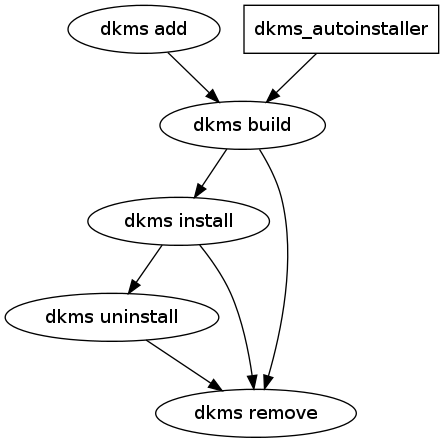
\includegraphics[width=0.4\hsize]{image201202/dkms.png}
 \end{center}
\label{fig:dkms}\caption{DKMS $BA4BN$NN.$l(B}
\end{figure}

dkms\_autoinstaller $B$O%7%9%F%`5/F0;~$K8F$P$l$k(B
\footnote{$B%G%#%9%H%j%S%e!<%7%g%s$K$h$C$F0[$J$k(B}$B%9%/%j%W%H$G$9!#(B
$B4{$K(B DKMS $B$KEPO?!J(Bdkms add$B!K$5$l$F$$$k%I%i%$%P%b%8%e!<%k$NCf$G!"(B
$B8=:_5/F0$7$F$$$k%+!<%M%kMQ$K%I%i%$%P%b%8%e!<%k$,%$%s%9%H!<%k(B
$B!J(Bdkms install$B!K$5$l$F$$$J$$$b$N$,$"$l$P!"(B
$B%I%i%$%P%b%8%e!<%k$N%S%k%I$H%$%s%9%H!<%k(B
$B!J(Bdkms build / dkms install$B!K$,<B9T$5$l$^$9!#(B

\subsubsection{$B%b%8%e!<%k%=!<%9%3!<%I$NG[CV0LCV(B}

DKMS $BBP1~%b%8%e!<%k$N%=!<%9%3!<%I$O(B
\url{/usr/src/$B%I%i%$%P%b%8%e!<%kL>(B-$B%P!<%8%g%s(B/} $B0J2<$KG[CV$9$kI,MW$,$"$j$^$9!#(B
$B@h$N%I%i%$%P$N>l9g!"(B\url{/usr/src/hello-0.0.1/} $B0J2<$KG[CV$7$^$9!#(B

\subsubsection{DKMS $B@_Dj%U%!%$%k(B}

DKMS $B$O!"3F%I%i%$%P%Q%C%1!<%8Kh$K@_Dj%U%!%$%k$r;}$DI,MW$,$"$j$^$9!#(B
$B$3$N@_Dj%U%!%$%k$G$O!"$I$N$h$&$J%I%i%$%P$,Ds6!!"%S%k%I!"%$%s%9%H!<%k$5$l$k$N$+(B
$B5-=R$5$l$F$$$kI,MW$,$"$j$^$9!#0J2<$K$h$/MxMQ$9$k@_Dj9`L\$r<($7$^$9!#(B
\begin{table}[ht]
 \caption{DKMS $B@_Dj%U%!%$%k9`L\(B}
 \label{tab:dkms-config-file}
\begin{center}
  \begin{tabular}{|l|p{35zw}|}
 \hline
 $B@_Dj9`L\(B & $BFbMF(B \\
 \hline \hline
PACKAGE\_NAME & $B%Q%C%1!<%8L>(B \\
PACKAGE\_VERSION & $B%Q%C%1!<%8%P!<%8%g%s(B \\
CLEAN & $B%-%c%C%7%e$J$I$N0l;~%U%!%$%k$r:o=|$9$k$?$a$N%3%^%s%I$r;XDj$9$k!#(B
       $B;XDj$7$J$$>l9g$K$O(B ``make clean '' $B$,<B9T$5$l$k!#(B\\
MAKE & $B%b%8%e!<%k$r%S%k%I$9$k%3%^%s%I$r;XDj$9$k!#(B\\
BUILT\_MODULE\_NAME & $B%I%i%$%P%b%8%e!<%k$NL>A0$r;XDj$9$k!J3HD%;R$OI,MW$J$7!K!#(B\\
BUILT\_MODULE\_LOCATION &  $B%S%k%I$5$l$?%b%8%e!<%k$,:n@.$5$l$k%G%#%l%/%H%j$^$G$NAjBP%Q%9(B\\
DEST\_MODULE\_LOCATION & $B%b%8%e!<%k$r%$%s%9%H!<%k$9$k%G%#%l%/%H%j$r;XDj$9$k!#(B\\
AUTOINSTALL & $B%b%8%e!<%k$r<+F0E*$K%$%s%9%H!<%k$9$k$+!"(B``yes'' $B$+(B ``no'' $B$r;XDj$9$k!#(B\\
REMAKE\_INITRD & $B%I%i%$%P%$%s%9%H!<%k;~$K(B initrd $B%$%a!<%8$r:F9=@.$9$k$+!"(B``yes'' $B$+(B ``no'' $B$r;XDj$9$k!#(B \\
PATCH & $BE,MQ$7$?$$%Q%C%A$r;XDj$9$k!#(B\\
PATCH\_MATCH & $B%Q%C%A$rE,MQ$9$k%P!<%8%g%s$N;XDj$9$k!#(BLinux $B%+!<%M%k$,(B 2.6.38 $B$H(B 2.6.39 $B$N>l9g$K%Q%C%A$rE,MQ$7$?$$>l9g$K$O(B ``\verb!2\.6\.(38|39)!'' $B$H;XDj$9$k!#(B\\
 \hline
 \end{tabular}
\end{center}
\end{table}

BUILT\_MODULE\_LOCATION $B$d(B BUILT\_MODULE\_NAME $B$J$I$O(B
$BG[Ns$r;H$C$F%I%i%$%P%b%8%e!<%kKh$K@_Dj$G$-$^$9!#(B
BUILT\_MODULE\_NAME $BG[Ns$NHV9f$O3FMWAG$NHV9f$KI3$E$$$F$$$k$N$G!"(B
$B=hM}$5$l$k$H$-$O3F!9$NHV9f$,;2>H$5$l$^$9!#(B
$BNc$($P!"0l$D$N%I%i%$%P%Q%C%1!<%8$+$i(B foo $B$H(B bar $B$N#2$D$N%G%P%$%9%I%i%$%P(B
$B$,Ds6!$5$l$k>l9g!"0J2<$N$h$&$K@_Dj$9$k$3$H$,$G$-$^$9!#(B

\begin{commandline}
$B!J>JN,!K(B
BUILT_MODULE_NAME[0] = "foo"
BUILT_MODULE_LOCATION[0]  = "foo_build"
DEST_MODULE_LOCATION[0] = "/update"
BUILT_MODULE_NAME[1] = "bar"
BUILT_MODULE_LOCATION[1]  = "bar_build"
DEST_MODULE_LOCATION[1] = "/update"
$B!J>JN,!K(B
\end{commandline}

$B$3$l$K$h$j!"%I%i%$%P(B foo $B$N%S%k%I$O(B foo\_build $B%G%#%l%/%H%j$G9T$o$l!"(B
update $B%G%#%l%/%H%j0J2<$K%$%s%9%H!<%k!"%I%i%$%P(B bar $B$N%S%k%I$O(B
bar\_build $B%G%#%l%/%H%j$G9T$o$l!"(Bupdate $B%G%#%l%/%H%j0J2<$K%$%s%9%H!<%k(B
$B$5$l$^$9!#(B

\subsubsection{DKMS $B$GDs6!$5$l$k%3%^%s%I(B}
DKMS $B$O(B dkms $B%3%^%s%I$GA`:n$7$^$9!#(B
$B0J2<$KMxMQIQEY$,9b$$%3%^%s%I$r>R2p$7$^$9!#(B

\begin{enumerate}
\item dkms status\\
DKMS $B$GDs6!$5$l$F$$$k(B $B%b%8%e!<%k$N%9%F!<%?%9$rI=<($7$^$9!#(B
\begin{commandline}
$ dkms status
v4l2loopback, 0.5.0, 3.1.0-1-amd64, x86_64: installed
v4l2loopback, 0.5.0, 3.2.0-1-amd64, x86_64: installed
virtualbox, 4.1.8, 3.1.0-1-amd64, x86_64: installed
virtualbox, 4.1.8, 3.2.0-1-amd64, x86_64: installed
\end{commandline}
%$

\item dkms add \\
$B%b%8%e!<%k$N%=!<%9%3!<%I$r4IM}BP>]$KDI2C$7$^$9!#(B
$B<B9T$9$k;~$K(B -m $B%*%W%7%g%s$GDI2C$9$k%I%i%$%P%Q%C%1!<%8L>$r!"(B
-v $B%*%W%7%g%s$G%P!<%8%g%s$r;XDj$7$^$9!#(B

\begin{commandline}
$ sudo dkms add -m hello -v 0.0.1

Creating symlink /var/lib/dkms/hello/0.0.1/source ->
                 /usr/src/hello-0.0.1

DKMS: add completed.
$ dkms status
hello, 0.0.1: added
\end{commandline}
%$

$B<B9T$9$k$H(B/var/lib/dkms $B0J2<$K(B $B%7%s%\%j%C%/%j%s%/$rD%$j!"(BDKMS $B$,4IM}$9$k(B
$B%I%i%$%P%G!<%?%Y!<%9$KEPO?$5$l$^$9!#(B

\item dkms build \\
$B4IM}BP>]$K$J$C$F$$$k%b%8%e!<%k$r%S%k%I$7$^$9!#(B
$B<B9T$9$k;~$K(B -m $B%*%W%7%g%s$GDI2C$9$k%I%i%$%P%Q%C%1!<%8L>$r!"(B
-v $B%*%W%7%g%s$G%P!<%8%g%s$r;XDj$7$^$9!#(B

$B%I%i%$%P$O(B \url{/var/lib/dkms/$B%I%i%$%PL>(B/$B%I%i%$%P%P!<%8%g%s(B/BUILT\_MODULE\_LOCATION} $B0J2<(B
$B$G%S%k%I$5$l$^$9!#(B
$B:n@.$5$l$?%b%8%e!<%k$H%S%k%I%m%0$O(B
\url{/var/lib/dkms/$B%I%i%$%PL>(B/$B%I%i%$%P%P!<%8%g%s(B/$B%+!<%M%k%P!<%8%g%s(B/$B%"!<%-%F%/%A%c(B}
$B0J2<$KCV$+$l$^$9!#(B

\begin{commandline}
$ sudo dkms build -m hello -v 0.0.1

Kernel preparation unnecessary for this kernel.  Skipping...

Building module:
cleaning build area....
make KERNELRELEASE=3.0.0-1-amd64 -C /lib/modules/3.0.0-1-amd64/build M=/var/lib/dkms/hello/0.0.1/build....
cleaning build area....
\end{commandline}
% $

\item dkms install\\
dkms build $B%3%^%s%I$K$h$C$F%S%k%I$5$l$?%b%8%e!<%k$r(Bdkms.conf $B$N(B
DEST\_MODULE\_LOCATION $B$G;XDj$5$l$F$$$k>l=j$K%$%s%9%H!<%k$7$^$9!#(B
$BNc$($P(B Linux $B%+!<%M%k(B 3.2.0-1-amd64 $B$r;H$C$F$$$F!"(B
\begin{commandline}
DEST_MODULE_LOCATION[0]="/updates"
\end{commandline}

$B$H;XDj$5$l$F$$$k>l9g$K$O(B \url{/lib/modules/3.2.0-1-amd64/updates/dkms/}
$B0J2<$K%$%s%9%H!<%k$5$l$^$9!#(B

\begin{commandline}
$ sudo dkms install -m hello -v 0.0.1

hello:
Running module version sanity check.
 - Original module
   - No original module exists within this kernel
 - Installation
   - Installing to /lib/modules/3.0.0-1-amd64/updates/dkms/

depmod..........

DKMS: install completed.
$ dkms status
hello, 0.0.1: installed
$ sudo modprobe -l | grep hello.ko
updates/dkms/hello.ko
\end{commandline}
%$

\item dkms uninstall\\
$B%b%8%e!<%k$r%"%s%$%s%9%H!<%k$7$^$9!#(B
$B<B9T$9$k;~$K(B -m $B%*%W%7%g%s$GDI2C$9$k%I%i%$%P%Q%C%1!<%8L>$r!"(B
-v $B%*%W%7%g%s$G%P!<%8%g%s$r;XDj$7$^$9!#(B
$B$^$?A4$F$N%+!<%M%k$+$i:o=|$9$k>l9g$K$O(B --all $B%*%W%7%g%s!"(B
$BFCDj$N%+!<%M%k%b%8%e!<%k$N$_$r:o=|$9$k>l9g$K$O(B -k $B%*%W%7%g%s$G%+!<%M%k(B
$B%P!<%8%g%s$r;XDj$7$^$9!#(B

\begin{commandline}
$ sudo dkms uninstall -m hello -v 0.0.1 -k 3.0.0-1-amd64

-------- Uninstall Beginning --------
Module:  hello
Version: 0.0.1
Kernel:  3.0.0-1-amd64 (x86_64)
-------------------------------------
$B!JCfN,!K(B

depmod....

DKMS: uninstall completed.
\end{commandline}
%$

% $BCfN,ItJ,(B
\if 0

Status: Before uninstall, this module version was ACTIVE on this kernel.

hello.ko:
 - Uninstallation
   - Deleting from: /lib/modules/3.0.0-1-amd64/updates/dkms/
 - Original module
   - No original module was found for this module on this kernel.
   - Use the dkms install command to reinstall any previous module version.

\fi

\footnote{$B$3$N;qNA$r:n@.$7$F$$$k;~E@$G$O!"!V(Bdkms uninstall$B!W$OF0:n$7$^$;$s!#(B
$B0lIt$N%A%'%C%/$,L$<BAu$J$?$a!"(Buninstall $B$N=hM}$^$G9T$o$l$J$$$?$a$G$9!#(B
\url{http://bugs.debian.org/cgi-bin/bugreport.cgi?bug=659672}}

\item dkms remove\\
DKMS $B$N4IM}BP>]$+$i30$7$^$9!#(Buninstall $B$HF1MM$N%*%W%7%g%s$,I,MW$G$9!#(B
$B%I%i%$%P%b%8%e!<%k$,%"%s%$%s%9%H!<%k$5$l$F$$$J$$>l9g!"%"%s%$%s%9%H!<%k$r<B9T$7$F$+$i!"(B
$B4IM}BP>]$+$i30$l$k$h$&$K$J$C$F$$$^$9!#(B

\begin{commandline}
$ dkms status
hello, 0.0.1, 3.0.0-1-amd64, x86_64: installed
virtualbox, 4.1.6, 3.0.0-1-amd64, x86_64: installed
$ sudo dkms remove  -m hello -v 0.0.1 --all

-------- Uninstall Beginning --------
Module:  hello
Version: 0.0.1
Kernel:  3.0.0-1-amd64 (x86_64)
-------------------------------------
$B!JCfN,!K(B

depmod....

DKMS: uninstall completed.

------------------------------
Deleting module version: 0.0.1
completely from the DKMS tree.
------------------------------
Done.
$ dkms status
\end{commandline}
%$

% $BCfN,ItJ,(B
\if 0

Status: Before uninstall, this module version was ACTIVE on this kernel.

hello.ko:
 - Uninstallation
   - Deleting from: /lib/modules/3.0.0-1-amd64/updates/dkms/
 - Original module
   - No original module was found for this module on this kernel.
   - Use the dkms install command to reinstall any previous module version.


\fi

\end{enumerate}

$B$=$NB>!"(Brpm $B%Q%C%1!<%8$r:n@.$9$k(B mkrpm $B%*%W%7%g%s$d(B Debian$B%Q%C%1!<%8(B
$B$r:n@.$9$k(B mkdeb $B%*%W%7%g%s$J$I$,MQ0U$5$l$F$$$^$9!#(B

\subsection{DKMS $BBP1~(BDebian $B%Q%C%1!<%8$N:n$jJ}(B}

$B>e5-$G$N@bL@$N$h$&$K!"(BDKMS $BBP1~%b%8%e!<%k$N%=!<%9$r5,Dj$N%G%#%l%/%H%j$K(B
$BE83+$7$F$*$/$H(B DKMS $B$O=hM}$r9T$$$^$9!#(BDebian $B$N>l9g$b%Q%C%1!<%82=$9$k$H$-$O(B
$B%$%s%9%H!<%k$7$?;~$K5,Dj$N%G%#%l%/%H%j$KE83+$9$k$h$&$K$7$F$*$-$^$9!#(B
$B%Q%C%1!<%8L>$J$I$K4X$7$F$O%k!<%k$,7h$^$C$F$*$j!"(B DKMS $BBP1~%Q%C%1!<%8$O(B
-dkms $B$H$$$&%5%U%#%C%/%9$,$D$$$F$$$^$9!#(B
$B$3$l$O%Q%C%1!<%8L>$,$o$+$j$d$9$$$H$$$&M}M3$H!"(BDKMS $BMQ$N(B debhelper
$B%3%^%s%I!"(Bdh\_dkms $B%3%^%s%I$,(B -dkms $B%5%U%#%C%/%9$N$D$$$?%Q%C%1!<%8$K(B
$BBP$7$F=hM}$r9T$&$?$a$G$9!#(B
debian/$B%Q%C%1!<%8L>(B.dkms $B$^$?$O(B debian/dkms $B$r(B dkms.conf $B$KJQ49$7$F!"(B
$BE,@Z$J(B dkms $BMQ%G%#%l%/%H%j$K%3%T!<$7!"(Bpostinst $B$H(B prerm $B$K(B DKMS $BMQ$N(B
$B=hM}$rDI2C$7$^$9!#(B
dh\_dkms $B%3%^%s%I$O(B dkms $B%Q%C%1!<%8$GDs6!$5$l$F$$$^$9!#(B
debhelper 7 $B0J9_$GMxMQ$9$k>l9g$K$O!"%"%I%*%s$H$7$FFI$_9~$^$;$kI,MW(B
$B$,$"$j$^$9!#(B

debian/hello-dkms.dkms:
\begin{commandline}
PACKAGE_NAME="hello"
PACKAGE_VERSION="#MODULE_VERSION#"
BUILT_MODULE_NAME[0]="$PACKAGE_NAME"
BUILT_MODULE_LOCATION="src"
DEST_MODULE_LOCATION[0]="/updates"
AUTOINSTALL="yes"
\end{commandline}
%$

DKMS $BMQ(B debian/rules:
\begin{commandline}
#!/usr/bin/make -f

VERSION := $(shell dpkg-parsechangelog | sed -nr '/^Version:/s/Version: (.*:)?(.*)-(.*)/\2/p')

%:
    dh $@ --with dkms
override_dh_install:
    dh_install src/* usr/src/hello-$(VERSION)/src/
    dh_install Makefile usr/src/hello-$(VERSION)/
override_dh_dkms:
    dh_dkms -V $(VERSION)

override_dh_auto_configure override_dh_auto_build override_dh_auto_test override_dh_auto_install override_dh_auto_clean:
\end{commandline}
%$

debian/rules $B%U%!%$%kFb$G(B override\_dh\_auto\_configure $B$d(B
override\_dh\_auto\_build $B$r8F$S=P$7$F$$$kM}M3$O(B Makefile $B$,$"$k>l9g!"(B
make $B$,<B9T$5$l$F$7$^$&$N$G$3$l$rM^@)$9$k$?$a$G$9!#(B

\subsubsection{Debian $B$G$N%I%i%$%P%b%8%e!<%k%S%k%I$N%?%$%_%s%0(B}

Debian $B$G$O(B DKMS $B%I%i%$%P%Q%C%1!<%8$,%$%s%9%H!<%k$5$l$?8e$H!"(B
$B%+!<%M%k%X%C%@(B $B$^$?$O(B $B%+!<%M%k%$%a!<%8%Q%C%1!<%8$,%$%s%9%H!<%k(B
$B!J99?7!K$5$l$?8e!"(B dkms $B$,5/F0$7$F%I%i%$%P%b%8%e!<%k$N%3%s%Q%$%k$,9T$o$l$k$h(B
$B$&$K$J$C$F$$$^$9!#$3$l$i$O0J2<$N%U%!%$%k$G=hM}$5$l$^$9!#(B

\begin{commandline}
/etc/kernel/postinst.d/dkms
/etc/kernel/header_postinst.d/dkms
\end{commandline}

\subsubsection{Debian $B$N(B DKMS $BBP1~>u67(B}

$B<gMW$J%I%i%$%P$NKX$I$O(B DKMS $B$H(B module-assistant$B!J0J2<(B m-a$B!K$NN>J}(B
$B$KBP1~$7$F$$$^$9!#3+H/$,$"$^$j3hH/$G$O$J$$%I%i%$%P$O(B m-a $B$N$_(B
$B$r%5%]!<%H$7$?>uBV$,B?$$$h$&$G$9!#(B
$B?7$7$/%Q%C%1!<%82=$5$l$?%I%i%$%P$O$[$H$s$I$,N>J}$KBP1~$7$F$$$^$9!#(B
DKMS $B$N$[$&$,%a%j%C%H$,B?$$$?$a!"(Bm-a $B$+$i(B DKMS $B$K@Z$jBX$($F$$$k%f!<%6(B
$B$bB?$$$h$&$G$9!#(B

\subsection{module-assistant $B$H$N0c$$(B}
Debian $B$K$OB>$N%I%i%$%P%Q%C%1!<%84IM}5!9=$K(B
module-assistant$B!J(Bm-a$B!K$,$"$j$^$9!#(B
DKMS $B$H(B m-a $B$N0c$$$K$O0J2<$N$h$&$K$J$C$F$$$^$9!#(B
\begin{itemize}
\item m-a $B$O<+F0%S%k%I5!9=$,$J$$!#(B\\
$B%+!<%M%k$,99?7$5$l$k$H!"<jF0$G(B m-a $B$r<B9T$9$kI,MW$,$"$j$^$9!#(B
\item DKMS $B$O%I%i%$%PMQ$N%P%$%J%j%Q%C%1!<%8$r:n$i$J$$!#(B\\
m-a $B$O(B $B%+!<%M%kKh%P%$%J%j%Q%C%1!<%8$r:n$j!"$=$l$r%$%s%9%H!<%k$7$^$9!#(B
\item m-a $B$O5/F0$7$F$$$k%+!<%M%k$N$_$N%I%i%$%P$r%S%k%I$9$k$,!"(BDKMS $B$O(B
$B%$%s%9%H!<%k$5$l$F$$$k%+!<%M%k$r%S%k%I$G$-$k!#(B
\end{itemize}

\subsection{$B$^$H$a(B}

$B:#2s$O(B DKMS $B$N4pK\E*$J;EAH$_$H!"(BDebian $B$G$N(B DKMS $BBP1~%Q%C%1!<%8:n@.J}K!(B
$B$K$D$$$F@bL@$7$^$7$?!#:#$^$G$O(B m-a $B$,<gN.$@$C$?$N$G$9$,(B DKMS $B$b%5%]!<%H(B
$B$7$F$$$k%I%i%$%P%Q%C%1!<%8$bA}$(;O$a!"=y!9$K(B DKMS $B$K0\9T$7$D$D$"$k$h$&$K(B
$B46$8$^$7$?!#(BDebian$B%Q%C%1!<%8MQ%D!<%k$,MQ0U$5$l$F$$$k$?$a!"(B
$BBP1~%Q%C%1!<%8:n@.$bFq$7$/$J$$$H;W$$$^$9!#(B
$B:#8e%I%i%$%P%Q%C%1!<%8$r:n@.$9$k>l9g$K$O!"(BDKMS $B$r%5%]!<%H$7$F$_$F$O(B
$B$$$+$,$G$7$g$&$+!#(B

\clearpage

%-------------------------------------------------------------------------------
\dancersection{$B$5$-$,(B(ry NM $B=N(B}{$BARI_8g(B}
%-------------------------------------------------------------------------------
\index{NM}
\index{New Member}

\subsection{NM $B$H$O2?$+(B}

Debian $B$K$*$1$k(B NM (New Member) $B$H$O!"?7$7$/(B Debian Project $B$N;22C%a%s%P!<$K$J$C$??M!"$"$k$$$O(B Debian Project
$B$K;22C$9$k$?$a$N<jB3$-!"$H$$$C$?0UL#$G;H$o$l$^$9!#8e<T$N>l9g$O!"0UL#$rL@3N$K$9$k$?$a$K!"(BNM $B%W%m%;%9$H$$$C$?$j$b$7$^$9!#(B
$B>/$7A0$^$G$O!"(BNew Maintainer $B$NN,$@$C$?$N$G$9$,!"(B($B%Q%C%1!<%8(B) $B%a%s%F%J0J30$K$bLg8M$r3+$3$&!"$H$$$&J}8~@-$KJQ99$5$l$D$D$"$j$^$9(B
($B$H$O$$$(!"8=;~E@$G$O(B NM $B%W%m%;%9$O$^$@%Q%C%1!<%8%a%s%F%J$rG0F,$K$*$$$?7A$N$^$^$G$9(B)$B!#(B

\subsection{NM$B%W%m%;%9$N>R2p(B}

$B$G$O!"<B:]$N(BNM$B%W%m%;%9$r<BNc$r$b$H$K$4>R2p$7$^$9!#K\Ev$O$b$&>/$7%W%m%;%9$r?J$a$F$*$/$D$b$j$@$C$?$N$G$9$,!"$"$^$j%9%`!<%:$K$$$C$F$J$$$N$GESCf$^$G$K$J$C$F$$$^$9!#(B

NM $B;V4j<T8~$1$N%A%'%C%/%j%9%H(B (http://www.debian.org/devel/join/nm-checklist) $B$,$"$j$^$9$N$G!"$^$:$O$3$l$r8+$F$_$^$7$g$&!#(B

\subsubsection{$BI,MW$J>r7o(B}

$B$^$:!"(BDebian Developer$B!J0J2<(BDD$B!K(B 2 $BL>0J>e$H%-!<%5%$%s$7$F$$$k$3$H!"$5$i$K(B NM $B$X$N1~Jg$r?dA&$7$F$/$l$k(B DD $B$,(B 1 $BL>0J>e$$$k$3$H!"(B
$B$3$l$O6qBNE*$+$D:GDc8B$N>r7o$K$J$j$^$9!#(B
$B2C$($F!"$9$G$K(B Debian $B$K4X$o$k$"$kDxEY$N3hF0$r$7$F$-$F$$$k$3$H$bI,MW$H$5$l$^$9$,!"$3$l$K$D$$$F$OL@3N$J@~0z$-$,$"$k$o$1$G$O$"$j$^$;$s$7!":#8eJQ2=$7$F$/$kItJ,$J$N$G?eJ*$H$$$C$F$$$$$G$7$g$&!#(B

$B;d$NNc$@$H!"$^$H$b$K(B Debian $B$G$N3hF0$r$O$8$a$?$N$O(B 2007 $BG/$/$i$$$@$C$?$H;W$&$N$G!"$*$*$h$=(B 4 $BG/4V!"2<@Q$_$H$7$F%Q%C%1!<%8%a%s%F!"K]Lu!"%m!<%+%k%3%_%e%K%F%#3hF0$r$7$F$-$F$$$^$9$,!"$3$l$O$A$g$C$HD9$+$C$?(B (NM $B1~Jg$,CY$+$C$?(B) $B$+$J$!!"$H;W$C$F$$$^$9!#(B

$B:G6a$G$O!"(BDM $B$N%9%F%C%W$r$U$s$G$$$k$3$H$,?d>)$5$l$F$$$k$3$H$b$"$k$N$G!">/$J$/$H$b(B6$B%v7n0J>eFCDj$N%Q%C%1!<%8$r%a%s%F$7$F$$$F!"%9%]%s%5!<$HNI9%$J4X78$rC[$1$F$$$l$P!"$=$N$^$^(B NM $B$K?J$`$3$H$b2DG=$G$7$g$&!#(B

\subsubsection{$B<BNc(B}

\begin{itemize}
\item 2011/11 ($B;vA0%M%4(B)
\item 2011/12/04 apply
\item 2011/12/04 advocate checked by yyabuki
\item 2011/12/10 activity poll sent
\item 2011/12/11 pass frontdesk precheck
\item 2011/12/13 AM assigned to gwolf
\item 2011/12/16 AM assigned to laney
\item 2011/12/17 ID checked
\item 2011/12/25 (Philosophy and Procedure $B$d$j$H$jCf(B)
\end{itemize}

$B$3$N8e$KB3$/M=Dj$O!"<!$N$h$&$K$J$C$F$$$^$9!#(B

\begin{itemize}
\item Tasks and Skills
\item AM recommends to DAM
\item DAM Approval
\end{itemize}

\subsubsection{NM$B%F%s%W%l!<%H(B}

NM $BC4Ev%A!<%`$G$O!"<g$K(B AM $BC4Ev<T8~$1$N;qNA$H$7$F!":n6H%,%$%I$N%j%]%8%H%j$,MQ0U$7$F$$$^$9(B(\url{http://anonscm.debian.org/viewvc/nm/trunk/nm-templates/})$B!#<B$O!"$3$3$r8+$l$P!"$@$$$?$$2?$rJ9$+$l$k$N$+$O$o$+$C$F$7$^$$$^$9$N$G!"M==,$N$?$a$N;29M=q$H$7$F$O:GNI$N$b$N$@$H;W$o$l$^$9!#$?$@$7!"(BAM $B$K$h$C$F$O(B NM $B%F%s%W%l!<%H$r;H$o$J$$!"$H$$$&?M$b$$$^$9$N$G!"LU?.$O$7$9$.$J$$$h$&$K$7$^$7$g$&!#(B

\subsubsection{NM $B$H(B $BJY6/2q$H(B Debian JP}

Debian $BJY6/2q$G$O!"(BDebian Developer $B$r0i@.$9$k!"$rL\E*$H$7$F$"$2$F$$$^$9!#$G$9$N$G!"$=$N1?1D<gBN$G$"$k(B Debian JP $B$H$7$F$b!";Y1g3hF0$O$$$m$$$m$H$*$3$J$o$l$F$$$^$9!#6qBNE*$K$O!"(BGPG $B%-!<%5%$%s$N?d?J$d!"%9%]%s%5!<C5$7$N%5%]!<%H!"%Q%C%1!<%8%s%0%9%-%k$N650i!"$J$I$G$9!#@'HsM-8z$K3hMQ$7$F$/$@$5$$!#(B

\subsubsection{NM $B$H(B Debian Maintainer}

$BJY6/2q$G$b2?EY$+$H$j$"$2$F$$$^$9$,!"$$$-$J$j(B NM $B$OI_5o$,9b$$!"$H$$$&?M$N$?$a$K!"(BDM $B$H$$$&%9%F%C%W$,MQ0U$5$l$F$$$^$9!#$3$l$O!"$$$o$P!V8BDj$D$-$N(B Debian Developer$B!W$G$"$j!"%9%]%s%5!<$K$D$$$F$b$i$&$3$H$G<+J,$N%Q%C%1!<%8$r(B Debian $B$K4^$a$k$3$H$,$G$-$k?MC#$N$3$H$G$9!#(B

$B;vA0$N<B@S$H$7$F$o$+$j$d$9$$$3$H$d!"FbMF$,%5%V%;%C%H$K$J$C$F$$$k$3$H$b$"$j!"(BNM $B%W%m%;%9$K$*$$$F$b!";vA0$K(B DM $B$H$7$F3hF0$7$F$*$/$3$H$,6/$/?d>)$5$l$F$$$^$9!#(B

\subsection{$B:G8e$K(B}

\subsubsection{$B$J$<(B NM $B$K!)(B}

NM $B$K$J$k$3$H$N0U5A$r9M$($F$_$^$7$g$&!#D>@\E*$K$O!"<!$N$h$&$J%a%j%C%H$,$"$j$^$9!#(B

\begin{itemize}
\item $B%Q%C%1!<%8$r<+M3$K%"%C%W%m!<%I$G$-$k(B
\item LWN.net $B$N9XFI8"(B (sponsored by HP)
\item Project Leader $B$d(B GR $B$X$NEjI<(B
\item @debian.org $B%a!<%k%"%+%&%s%H(B
\end{itemize}

$B$"$k$$$O<c$$?M$G$"$l$P!"Hf3SE*L>A0$NCN$i$l$?%W%m%8%'%/%H$X$N;22C<+BN$d!"%W%m%8%'%/%H$K<+J,?'$r;}$A9~$a$k!"$H$$$C$?K~B-$b$"$k$+$b$7$l$^$;$s!#(B
$B$?$@!"(BNM $B%W%m%;%9$d$=$N8e$N3hF0$O!"$=$l$J$j$K<j4V$b5$NO$bI,MW$K$J$j$^$9!#$3$l$8$c0z$-$,B-$j$J$$!"$H$$$&?M$bB?$$$G$7$g$&!#(B

Debian $BJY6/2q$H$7$F$O!"A0=R$7$?$H$*$j!"(BNM $B$K1~Jg$7$h$&$H;W$($k?M:`$r0i@.$7$?$$!"$H$$$&;W$$$,$"$k$N$G$9$,!"$d$O$jF05!$NItJ,$K$D$$$F$O!"3'$5$s$=$l$>$l$NEz$($r8+=P$7$F$$$?$@$/$7$+$"$j$^$;$s!#(B

$B%9%i%$%I$NJ}$G$O!"0lNc$H$7$F!"FC$K5;=QE*$K=($G$?$b$N$r$b$C$F$$$k$o$1$G$b$J$/!"6H3&E*$K$ODjG/$KC#$7$F$7$^$C$?$*$C$5$s$,!"0lBN2?$r9M$($F(B NM $B$KD)@o$7$F$_$F$$$k$N$+!"4JC1$K>R2p$7$F$_$^$9!#;29M$K$J$l$P!#(B

\clearpage

%% -*-tex-*-
%%
%% Copyright (C) 2012 Hiroshi Kubo  all rights reserved.
%% $BK\;qNA$NCx:n8"$O!"Cx<T$G$"$k5WJ]Gn(B <h-kubo@geisya.or.jp> $B$K$"$j$^$9!#(B
%%
%% This document material is licensed under the GNU General Public License version 2.0.
%% This document is originally in the form of LaTeX source code. This shall be referenced as the ``Corresponding Source''
%% Any compiled forms including DVI, Postscript, and PDF from the original source code shall be reference as the ``Object code''.
%%

%-------------------------------------------------------------------------------
\dancersection{$B%U%j!<%=%U%H%&%'%"$H5:$l$k$?$a$NCx:n8"F~Lg(B}{$B;3>k9q$N=;?M(B $B5WJ]Gn(B}
%-------------------------------------------------------------------------------
\index{Free software}
\index{$B$A$g$5$/$1$s(B@$BCx:n8"(B}

\subsection{$BA0=q$-(B}

$B?M@8$N$$$-$,$+$j>e!"3d$H:G6a$K$J$C$FCx:n8"$NJY6/$r;O$a$k$3$H$K$J$j$^$7$?!#(B
$BK!N'$N@lLg2H$G$O$"$j$^$;$s$N$G!"<+?.$r;}$C$F$NH/I=$G$O$J$$$G$9$,!"(B
$B$_$J$5$s$H0l=o$K9M$($F$$$/$-$C$+$1$K$J$l$P$H;W$$$^$9!#(B

\subsection{$B$O$8$a$K(B}

$BF|K\$r4^$`B?$/$N9q$G!"%=%U%H%&%'%"$O!"@8$_=P$5$l$?;~$+$iCx:n8"$H$$$&8"Mx$NBP>]$K$J$C$F$$$^$9!#(B

$B$G$9$+$i!"%U%j!<%=%U%H%&%'%"$b!"@8$^$l$?;~$+$iC/$+$N$b$N!"$H$$$&$3$H$K$J$C$F$$$^$9!#(B
$B%U%j!<$G$"$C$F$bC/$+$N$b$N$G$"$k!"$H$$$&E@$G$O!"EP5-$5$l$?EZCO$O6u$-CO$G$"$C$F$bC/$+$N$b$N$G$"$k$N$H$K$F$$$k$+$bCN$l$^$;$s!#(B

$B%U%j!<%=%U%H%&%'%"$N@:?@$O!"0l2p$NMxMQ<T$,<+J,<+?H$N$?$a$K%=%U%H%&%'%"$r;H$&$3$H$r(B
$BK8$2$k$h$&$J$3$H$O:GBg8BHr$1$k$h$&$K$7$F$$$^$9$+$i!"<+J,<+?H$N$?$a$K%U%j!<%=%U%H%&%'%"$r;H$&8B$j!"(B
$BCN$i$J$/$F$b:$$C$?$3$H$K$O$J$j$^$;$s!#(B

$B$G$b!"$=$3$+$i0lJbF'$_=P$=$&$H$9$l$P!"C/$+$N$b$N$G$"$k$H$$$&$3$H$rB:=E$9$k$3$H$,5a$a$i$l$k$3$H$K$J$j$^$9!#(B
$B$3$NMW@A$O!"Cx:n8"K!$H!"$=$l$rA0Ds$H$9$k7@Ls$K4p$E$$$F$$$^$9!#(B

$B$=$3$G!"(BDebian Project $B$,G[I[$7$F$$$k$h$&$J%U%j!<%=%U%H%&%'%"$r07$&>lLL$r$$$/$D$+A[Dj$7$F!"(B
$B$=$3$KCx:n8"$H7@Ls$,$I$N$h$&$K4X$o$C$F$/$k$N$+!"2r$-L@$+$7$F$_$^$9!#$J$*!"F|K\$NCx:n8"K!$r85$K$7$F$*OC$7$^$9!#(B



\subsection{$BCNE*:b;:8"(B}

$B%=%U%H%&%'%"$,C/$+$N$b$N$G$"$k!"$H$O!"$I$&$$$&$3$H$G$7$g$&!#(B

$BCNE*$J:n6H$rDL$7$FAO$j=P$5$l$?!"L5BNJ*!J%W%m%0%i%`$r4^$`!K$K$O!"(B
$BAO$j=P$7$??M$NEXNO$dO+NO$KJs$$$k$?$a$K!"$5$^$6$^$J@)EY$rDj$a$kK!N'$,@0Hw$5$l$F$$$^$9!#(B
$B$=$NCf$G$b!"CNE*$JAOB$$K$h$C$F$D$/$j=P$5$l$?L5BNJ*$KBP$7$F!"(B
$B:b;:8"$NBP>]$H$J$kM-BNJ*$NJ*8"$KNI$/;w$?8"Mx$r@_Dj$9$k;EAH$_$,K!N'$GDj$a$i$l$F$$$^$9!#(B
$B$3$NJ*8"$K;w$?8"Mx$rCNE*:b;:8"$H$$$$$^$9!#(B
$B$=$7$F!"CNE*:b;:8"$O!"AOB$$7$??M$"$k$$$OEPO?$7$??M$,5}<u$9$k8"Mx$J$N$G$9!#(B

$B$3$l$,!"%=%U%H%&%'%"$,C/$+$N$b$N$G$"$k!"$H$$$&$3$H$N!"8=Be<R2q$K$*$1$k0UL#$G$9!#(B

$B%=%U%H%&%'%"$,4X78$9$kCNE*:b;:8"$K$O!"<!$N$b$N$,$"$j$^$9!#(B

\begin{itemize}
\item[{\bf{$BCx:n8"(B}}] $B!V;WA[Kt$O46>p$rAO:nE*$KI=8=$7$?$b$N$G$"$D$F!"J87]!"3X=Q!"H~=QKt$O2;3Z$NHO0O$KB0$9$k$b$N!W$KBP$9$kFH@jE*$JJ]8n$r$b$?$i$98"Mx(B
\item[{\bf{$BFC5v8"(B}}]  $BH/L@!J<+A3K!B'$rMxMQ$7$?5;=QE*;WA[$NAO:n$N$&$A!"9bEY$J$b$N!K$rEPO?$9$k$3$H$K$h$C$FFH@jE*$JJ]8n$r$b$?$i$98"Mx(B
\item[{\bf{$B<BMQ?70F8"(B}}] $B9M0F!J<+A3K!B'$rMxMQ$7$?5;=QE*;WA[$NAO:n!K$rEPO?$9$k$3$H$K$h$C$FFH@jE*$JJ]8n$r$b$?$i$98"Mx(B
\item[{\bf{$B0U>"8"(B}}] $B0U>"!JJ*IJ$N7A>u!"LOMM<c$7$/$O?':L$^$?$O$3$l$i$N7k9g$G$"$C$F!";k3P$rDL$8$FH~46$r5/$3$5$;$k$b$N!K$rEPO?$9$k$3$H$K$h$C$FFH@jE*$JJ]8n$r$b$?$i$98"Mx(B
\item[{\bf{$B>&I88"(B}}] $B>&I8$rEPO?$9$k$3$H$K$h$C$FFH@jE*$JJ]8n$r$b$?$i$98"Mx(B
\end{itemize}

$B%W%m%0%i%`$=$N$b$N$O!"Cx:n8"$NBP>]$K$J$j$^$9!#(B
$B$^$?!"%W%m%0%i%`$G<BAu$5$l$?%"%k%4%j%:%`$OFC5v$d<BMQ?70F$NJ]8n$NBP>]$K$J$jF@$k>l9g$,$"$j$^$9$7!"%W%m%0%i%`$NL>>N$d%m%4$O>&I8$H$7$F$NJ]8n$NBP>]$K$J$jF@$^$9(B\footnote{Debian $B$bEE;R7W;;5!$J$I$N;XDj>&IJ$G$N>&I8EPO?$,$5$l$F$*$j!"EPO?HV9f$O(B $BBh#4#5#9#5#2#8#89f$G$9!#$A$J$_$K!";XDj>&IJ!V2[;R!"%Q%s!W$G!V%G%S%"%s!W$H$$$&>N8F$NEPO?HV9fBh#1#7#0#8#0#3#29f$NEPO?>&I8$,$"$j$^$9!#LLGr$$$G$9$M!#(B}$B!#(B
GUI$B$N2hLL$N%G%6%$%s$O3$30$G$O0U>"EPO?$NBP>]$H$J$jF@$k>l9g$b$"$k$h$&$G$9$,!"F|K\$G$O:#$N$H$3$mBP>]$G$O$"$j$^$;$s!#(B

$B$3$NCf$G$b!"%=%U%H%&%'%"$K$D$$$F0lHV$h$/LdBj$K$J$k$N$O!"Cx:n8"$G$9!#(B

\subsection{$BCx:n8"(B}
\subsubsection{$BCx:n8"$N@-<A(B}

$B@53N$G$O$J$$$G$9$,C<E*$K8@$($P!"Cx:n8"K!$O!"Cx:nJ*$r:n$C$??M$KCx:nJ*$KBP$9$kFH@jE*$J8"Mx$rM?$($kK!N'$G$9!#(B
$B$=$NCx:n8"K!$GDj$a$i$l$F$$$kCx:n8"$K$O<!$N$h$&$J@-<A$,$"$j$^$9!#(B

\begin{itemize}
\item $BCx:nJ*$r:n$C$?$i!"H/@8$7$^$9!#(B
\item $BCx:nJ*$r8xI=$7$J$/$F$bH/@8$7$^$9!#(B
\item $B!JFC5v$H0c$C$F!"!KLr=j$KEPO?$7$J$/$F$bH/@8$7$^$9(B\footnote{$B$3$N$h$&$J8"Mx$NH/@8$N$5$;J}$rL5J}<0<g5A$H8@$$$^$9!#$J$*!"$+$D$F%"%a%j%+$O!"L5J}<0<g5A$G$O$"$j$^$;$s$G$7$?!#(B}$B!#(B
\item $BCx:nJ*$,@8$^$l$F$+$i!"Cx:n<T$N;`8e(B50$BG/4V!"Cx:n8"$NJ]8n$OB3$-$^$9!#(B
\item $BB>?M$,Cx:nJ*$r>!<j$KMxMQ$7$?>l9g!":9;_@A5a8"!"B;32Ge=~@A5a8"$r9T;H$9$k$H$$$&J}K!$GBP93$G$-$^$9(B\footnote{$BCx:n8"K!BhI4==;M>r$K4p$E$$$FB;323[$r?dDj$7$F$b!"%U%j!<%=%U%H%&%'%"$N>l9g!"(B0$B1_$K$7$+$J$i$J$$$G$9$,!D!#(B}$B!#(B
\end{itemize}
$B$G$9$+$i!"?7$7$$%W%m%0%i%`$,:n$i$l$l$P!"I,$:$H8@$C$F$$$$$[$ICx:n8"$,4X78$7$F$-$^$9!#(B

$B5U$K8@$($P!"Cx:nJ*$r%Q%V%j%C%/%I%a%$%s$H$9$k$?$a$K$O!"Cx:n8"$rJ|4~$9$k<jB3$-$J$I$,I,MW$K$J$k$o$1$G$9!#(B
$B$^$?!"Cx:nJ*$rMxMQ$9$k$K$O!"Cx:n8"<T$+$iMxMQ5vBz$r$b$i$&$Y$7!"$H$$$&$N$,Cx:n8"K!$KB'$C$?@5$7$$J}K!$G$9!#(B

$B$7$?$,$C$F!"%=%U%H%&%'%"$H$H$b$K(B
\begin{itemize}
\item $BCx:n8"$K4p$E$/MxMQ5vBz7@Ls=q(B
\item $BCx:n8"$rJ|4~$9$k@k8@$"$k$$$OJ|4~:Q$G$"$k$3$H$NL@<(E*$J@bL@(B
\end{itemize}
$B$N$I$A$i$+$r<j$KF~$l$J$$$H!"Cx:n8"K!$K0cH?$7$F$$$J$$3N?.$r;}$C$F%=%U%H%&%'%"$r;H$&$3$H$,Fq$7$$!"$H$$$&$3$H$K$J$j$^$9!#(B
Debian Project $B$O!"<R2q7@Ls(B\cite{DebianSocialContract}$B$K4p$E$$$F9TF0$7$F$*$j!"$3$NE@$K4X$7$F87L)$K9M$($F%Q%C%1!<%8$r:n$C$F$$$k$o$1$G$9!#(B

\subsubsection{$BCx:n8"$NB8B34|4V(B}

$B8"Mx$,M-8z$G$"$k;~4V$NHO0O$rB8B34|4V$H8@$$$^$9!#(B

$B!VCx:n<T$,;`$s$G$bCx:n8"$NJ]8n$,B3$/$C$F$I$&$$$&$3$H(B?$B!W$HIT;W5D$K;W$&$+$bCN$l$^$;$s$M!#(B
 $BCx:n8"$OAjB3$G$-$k$N$G$9!#AjB3$9$k?M$,$"$l$P!"B3$/$s$G$9!#(B
$BAjB3$r4^$a$F!"8"Mx$r0z$-7Q$0$3$H$r!V>57Q!W$H8@$$$^$9!#(B
$B>57Q$9$k?M$,$J$1$l$P!"Cx:n8"$O>CLG$7$^$9!#(B

\par
\begin{center}
\fbox{
\parbox{0.8\linewidth}{
\begin{center}{\Large\bf $BI.<T$+$i$*4j$$!*(B}\\
$B$"$J$?$,:n$C$F8x3+$7$F$$$k%W%m%0%i%`!"(B\linebreak[1]$B$"$J$?$N;`8e$KC/$,Cx:n8"$rAjB3$9$k$+M=$a<~$j$N?M$K65$($F$*$$$F2<$5$$!#(B
\end{center}
}
}
\end{center}
\par


$B$J$*!"(BFSF\footnote{Free Sofware Foundation. $B%&%'%V%5%$%H$O(B {\url http://www.fsf.org/}}$B$O!"(BFSF$B$XCx:n8"$r>yEO$9$k$3$H$r4+$a$F$$$^$9(B\cite{FSFassign}$B!#Cx:n<T$N;`8e!"(BGPL\footnote{GNU General Public License}$B$G8x3+$7$?%U%j!<%=%U%H%&%'%"$N9T$/Kv$rBw$9$3$H$b$G$-$^$9$M(B\footnote{$BCx:n8"$N>yEO$K4X$7$F$O!"F|K\$NCx:n8"K!$K$OBh;0<TBP93MW7o$KEPO?$,I,MW$J$I$NFq$7$$OC$,4X78$9$k$N$G!"I.<T$O$I$&$7$?$i$$$$$N$+!"M}2r$G$-$F$$$^$;$s!#(B}$B!#(B

\subsubsection{$BCx:n8"$NFbLu(B}

$BCx:n8"$H$O!"8"Mx$NB+$_$?$$$J$b$N$G$9!#Cx:nJ*$rMxMQ$9$kJ}K!$J$I$K$h$C$F!":Y$+$$8"Mx$,Dj$a$i$l$F$$$^$9!#(B

$B$=$l$i$OBgJL$9$k$H!"!VCx:n?M3J8"!W$H!VCx:n:b;:8"!W$KJ,$+$l!"$=$l$>$l$N2<$K<!$N$h$&$J8"Mx$,>rJ8$GDj$a$i$l$F$$$^$9!#(B

\begin{description}
\item[$BCx:n?M3J8"(B]$B!V8xI=8"!W!V;aL>I=<(8"!W!VF10l@-J];}8"!W(B
\item[$BCx:n8"!JCx:n:b;:8"!K(B]$B!VJ#@=8"!W!V>e1i8"!W!V1iAU8"!W!V>e1G8"!W!V8x=0Aw?.8"!W!VEAC#8"!W!V8}=R8"!W!VE8<(8"!W!VHRI[8"!W!V>yEO8"!W!VB_M?8"!W!VK]Lu8"!W!VK]0F8"!W!VFs<!E*Cx:nJ*$NMxMQ$K4X$9$k8"Mx(B $B!W(B
\end{description}

$B$3$NCf$K$O!"%=%U%H%&%'%"$,4X78$7$J$$$b$N$b$"$j$^$9!#(B

\subsection{Debian Project $B$,G[I[$7$F$$$k$b$N$N2?$,Cx:nJ*(B?}

$B$5$F!"Cx:nJ*$H$O$I$s$J$b$N$,$"$k$+!"Cx:n8"K!$rFI$s$G$_$k$H!"<!$N$h$&$J$3$H$,=q$$$F$"$j$^$9!#(B

$BCx:nJ*$H$O!"!V;WA[Kt$O46>p$rAO:nE*$KI=8=$7$?$b$N$G$"$D$F!"J87]!"3X=Q!"H~=QKt$O2;3Z$NHO0O$KB0$9$k$b$N$r$$$&!#!W(B
$B!JCx:n8"K!BhFs>r!K(B


$B99$K!"Cx:n8"K!$G$O!"Nc$r5s$2$FCx:nJ*$rDj5A$7$F$$$^$9!#(B

\begin{verbatim}
$BBh==>r!!$3$NK!N'$K$$$&Cx:nJ*$rNc<($9$k$H!"$*$*$`$M<!$N$H$*$j$G$"$k!#(B
$B!!(B 	$B0l!!>.@b!"5SK\!"O@J8!"9V1i$=$NB>$N8@8l$NCx:nJ*(B
$B!!(B 	$BFs!!2;3Z$NCx:nJ*(B
$B!!(B 	$B;0!!IqMYKt$OL58@7`$NCx:nJ*(B
$B!!(B 	$B;M!!3(2h!"HG2h!"D&9o$=$NB>$NH~=Q$NCx:nJ*(B
$B!!(B 	$B8^!!7zC[$NCx:nJ*(B
$B!!(B 	$BO;!!CO?^Kt$O3X=QE*$J@-<A$rM-$9$k?^LL!"?^I=!"LO7?$=$NB>$N?^7A$NCx:nJ*(B
$B!!(B 	$B<7!!1G2h$NCx:nJ*(B
$B!!(B 	$BH,!!<L??$NCx:nJ*(B
$B!!(B 	$B6e!!%W%m%0%i%`$NCx:nJ*(B

2$B!!;v<B$NEAC#$K$9$.$J$$;(Js5Z$S;~;v$NJsF;$O!"A09`Bh0l9f$K7G$2$kCx:nJ*$K3:Ev$7$J$$!#(B

3$B!!Bh0l9`Bh6e9f$K7G$2$kCx:nJ*$KBP$9$k$3$NK!N'$K$h$kJ]8n$O!"$=$NCx:nJ*$r:n@.$9$k$?$a$KMQ$$$k%W%m%0%i%`8@8l!"5,Ls5Z$S2rK!$K5Z$P$J$$!#$3$N>l9g$K$*$$$F!"$3$l$i$NMQ8l$N0U5A$O!"<!$N3F9f$KDj$a$k$H$3$m$K$h$k!#(B
$B!!(B 	$B0l!!%W%m%0%i%`8@8l(B $B%W%m%0%i%`$rI=8=$9$k<jCJ$H$7$F$NJ8;z$=$NB>$N5-9f5Z$S$=$NBN7O$r$$$&!#(B
$B!!(B 	$BFs!!5,Ls(B $BFCDj$N%W%m%0%i%`$K$*$1$kA09f$N%W%m%0%i%`8@8l$NMQK!$K$D$$$F$NFCJL$NLsB+$r$$$&!#(B
$B!!(B 	$B;0!!2rK!(B $B%W%m%0%i%`$K$*$1$kEE;R7W;;5!$KBP$9$k;XNa$NAH9g$;$NJ}K!$r$$$&!#(B
\end{verbatim}

$B$H$$$&$3$H$G!"%W%m%0%i%`$O!"%W%m%0%i%`Cx:nJ*$G$9!#%*%V%8%'%/%H%3!<%I$b%W%m%0%i%`Cx:nJ*$G$"$k!"$H$$$&H=Nc$b$"$k$h$&$G$9(B\footnote{$BEl5~COH=><OB(B60$BG/(B3$B7n(B8$BF|H=%?(B 561$B9f(B 169$BJG!V%G%#%0%@%0!W;v7o(B $B$H$$$&H=Nc$,$"$k$=$&$G$9(B\cite{saito}$B!#(B}$B!#(B

$B$^$?!"(BDebian Project $B$,G[I[$9$k$b$N$K$O%W%m%0%i%`0J30$K$b!"J8>O!"<L??2hA|!"CO?^%G!<%?$J$I$"$j$^$9$,!"Cx:nJ*$G$9!#(B


\subsection{$BCx:n8"$rF'$^$($?(B Debian Project $B$+$i$NG[I[J*$H$N$*$D$-9g$$(B}


\subsubsection{$BCx:n8"$N$3$H$r5$$K$;$:$K(B Debian $B$N%7%9%F%`$r%$%s%9%H!<%k$7$^$7$?!#2?$+$^$:$$$3$H$r$7$F$$$J$$$G$7$g$&$+(B?}

$B<+J,$G;H$&L\E*$G%$%s%9%H!<%k$7$?$N$G$9$h$M(B?

$B%$%s%9%H!<%k$9$kA0$KMxMQ5vBz7@Ls$rFI$s$G!"F10U$7$F!"$=$l$+$i%$%s%9%H!<%k$9$k$N$,M}A[E*$G$9$,!"$=$&$G$J$$>l9g$b$h$/$"$k$+$H;W$$$^$9!#(B

Debian Project $B$,G[$C$F$$$k%$%s%9%H!<%i!<$r;H$C$FIaDL$K%$%s%9%H!<%k$7$?$J$i!"(B
$B%$%s%9%H!<%k$7$?%=%U%H%&%'%"$NMxMQ5vBz7@Ls$KF10U$7$?$3$H$K$7$^$7$g$&!#(B
$B%$%s%9%H!<%i!<$G%$%s%9%H!<%k$7$?%=%U%H%&%'%"$O$9$Y$F(B DFSG\footnote{The Debian Free Software Guidelines\cite{DFSG}} $B$K=`5r$7$F$$$k$N$G!"$[$H$s$I$"$J$?$OITMx1W$rHo$C$F$$$^$;$s!#(B

\begin{itemize}
\item $B6bA,E*$JBP2A$OMW5a$5$l$^$;$s!#(B
\item $B;H$&$@$1$J$iL5=~$N9W8%$bMW5a$5$l$^$;$s!#(B
\item $B$"$J$?$NK?$+$N8"Mx$rJ|4~$7$?$jCGG0$7$?$j>yEO$7$?$j$9$k$3$H$b$"$j$^$;$s!#(B
\end{itemize}

$B$J$K$+5$$r$D$1$k$3$H$,$"$k$H$9$l$P!"LH@U>r9`$/$i$$$G$7$g$&$+!#(B

 $B$[$\$9$Y$F$N%U%j!<%=%U%H%&%'%"$NMxMQ5vBz$G$O!"$=$NF0:n$K4X$7$FL5J]>Z$G!"LH@U>r9`$,@9$j9~$^$l$F$$$^$9(B\footnote{$B%U%j!<$G$J$/$F$b!"L5J]>Z$G$"$k>l9g$,B?$$$G$9$7!"J]>Z$O$"$C$F$bGe=~3[$N>e8B$r%=%U%H%&%'%"9XF~Be6b$H$9$k$3$H$bDA$7$/$"$j$^$;$s!#(B}$B!#(B
$BL5J]>Z$G$"$k$3$H$K4X$9$kF10U$O!"$[$H$s$I$N%=%U%H%&%'%"$,:NMQ$7$F$$$kMxMQ5vBz$N7@Ls$N>r9`$N0lIt$G$9!#F10U$G$-$J$$$J$i!"MxMQ$9$k8"Mx$O$"$j$^$;$s!#(B

$B$7$?$,$C$F!"Cx:n<T$KBP$7$F!"<!$K7G$2$k$3$H$K$D$$$F2?$NJ86g$r$D$1$k6Z9g$$$b$"$j$^$;$s!#(B
\begin{itemize}
\item  $B4|BTDL$j$KF0$+$J$$(B
\item  $B$=$b$=$bF0$+$J$$(B
\item  $B%=%U%H%&%'%"$r;H$C$?$;$$$G!"CO0L$d:b;:$r<:$C$?(B
\item  $B%=%U%H%&%'%"$r?.$8$?$;$$$G!"CO0L$d:b;:$r<:$C$?(B
%%\item  $B%=%U%H%&%'%"$r;H$C$?$;$$$G!"?4$,=}$D$$$?(B
\end{itemize}

%% $B$3$3$G(B BTS $B$NOC$r0l@J(B
$B$G$b!"B?$/$N%U%j!<%=%U%H%&%'%"$N3+H/85$d(B Debian Project $B$K$O!"%P%0Js9p$NAk8}$,$"$j$^$9$M!#(B
$B$"$l$O!"5AL3$G$d$C$F$$$k$N$G$J$$$N$G$9!#Bg$$$J$k?F@Z0J30$N2?J*$G$b$"$j$^$;$s!#(B


%% \subsubsection{$BCN9g$$$N%Q%=%3%s$K(B Debian $B$N%7%9%F%`$r%$%s%9%H!<%k$7$^$7$?!#(B}

%% $B$=$N%Q%=%3%s$rMxMQ$9$k;}$A<g$NJ}$K!"MxMQ5vBz=q$KF10U$7$F$b$i$$$^$7$g$&!#(B
%% $BJL$K!"=qN`$KH=;R$r$D$/$h$&$J<jB3$-$OI,MW$"$j$^$;$s!#(B

%% $BA4It$rM}2r$7$F$b$i$&$N$O$J$+$J$+:$Fq$@$H$O;W$$$^$9$,!"(B
%% $B<+J,$N$?$a$K;H$C$F!"$&$^$/$$$+$J$/$F$b:n<T$NJ}!9$KJ86g$r$$$&6Z9g$$$O$J$$$3$H$KG<F@$7$F$b$i$($l$P<B:]>e$O==J,$G$9!#(B


\subsubsection{Debian $B$N%U%j!<%=%U%H%&%'%"$r;H$o$J$$$1$IG[$j$^$9!#(B}

$B$A$g$C$HBT$C$F(B! $B$"$J$?$O!"Cx:n<T$H7@Ls$r7k$P$J$/$F$O$J$j$^$;$s(B!

$BCx:n8"$K$O!VJ#@=8"!W!V<+F08x=0Aw?.8"!W!VAw?.2DG=2=8"!W$H$$$&8"Mx$,4^$^$l$F$$$k$N$G$9!#(B
$B6K$a$F4JC1$KJ,$+$j$d$9$/$$$&$H(B
\begin{description}
\item[$BJ#@=8"(B ] $B4JC1$K$$$&$H!"%3%T!<$9$k8"Mx!#(B
\item[$B<+F08x=0Aw?.8"(B] $B8x=0$KAw?.$9$k8"Mx!#(B
\item[$BAw?.2DG=2=8"(B] $B8x=0$,%"%/%;%9$7$F%@%&%s%m!<%I$G$-$k%5!<%P!<$KCx:nJ*$rCV$/8"Mx!#(B
\end{description}
$B$G$9!#(B
$BCx:n<T$,FH@jE*$KJ];}$9$k8"Mx$G$9$+$i!"$"$J$?$O!"%=%U%H%&%'%"$rG[$C$?$j!"8x3+$5$l$F$$$k%5%$%H$K%"%C%W%m!<%I$9$kA0$K$O!"Cx:n<T$N5v2D$,I,MW$G$9!#(B


$B$G$b<B$O!"(BDebian $B%"!<%+%$%V$N(B main $B%;%/%7%g%s$H(B contrib $B%;%/%7%g%s$K4^$^$l$k%=%U%H%&%'%"$N%=!<%9%3!<%I$r(B
{\em $B$=$N$^$^(B}$BL5NA$GG[I[$9$k>l9g$O!"MxMQ5vBz$KF10U$9$kI,MW$O$"$k$b$N$N!"(B
$B<B<AE*$K$O2?$i$+$N5AL3$d@)Ls$KG{$i$l$k$3$H$O$"$j$^$;$s$N$G!"(B
$B$[$H$s$I5$$K$+$1$kI,MW$O$J$$$G$9!#(B

$B$H$$$&$N$b!"(Bmain $B$H(B contrib $B$K4^$^$l$k%=%U%H%&%'%"$O!"$9$Y$F(B DFSG\cite{DFSG} $B$K=`5r$7$F$^$9!#(B
DFSG $B$K=`5r$7$F$$$k$3$H$$$&$3$H$O!"%=!<%9%3!<%I$N<+M3$JG[I[$,MxMQ5vBz7@Ls>e!"G'$a$i$l$F$$$k$3$H$K$J$k$N$G$9!#(B

$B$3$l$KBP$7$F!"%P%$%J%j%Q%C%1!<%8$rG[I[$9$k>l9g$O!"G[I[@h$G%=!<%9%3!<%I$,<j$KF~$l$k$3$H$,$G$-$k$h$&$KG[N8$7$J$$$H$$$1$J$$%i%$%;%s%9$,B?$$$G$9(B\footnote{GPL $B$d(B LGPL (GNU Lesser General Public License)  $B$,E57?E*$JNc$G$9!#(B}$B!#(B
$B%=!<%9%3!<%I$,F~<j$G$-$k$h$&$JG[I[$r6/@)$9$k$3$H$G!"%=%U%H%&%'%"$N<+M3$rC4J]$7$h$&$H$7$F$$$k$o$1$G$9!#(B
$BCm0U$7$^$7$g$&!#(B


$B$^$?!"MxMQ5vBz$NFbMF$rM}2r$9$kA0$K!"E,Ev$K0lIt$r:o$C$?$j!"0lIt$rH4$-=P$7$FG[$i$J$$$h$&$K$7$^$7$g$&!#(B
$B$H$$$&$N$b!"Cx:n8"$K$O!VF10l@-J];}8"!W$H$$$&8"Mx$,$"$j$^$9!#(B
$B>!<j$K:o$k$3$H$b4^$a$F!"Cx:nJ*$r>!<j$K2~JQ$9$k$3$H$OCx:n8"K!$,6X$8$F$$$^$9!#(B
$B2~JQ$K:]$7$F$O5vBz$,I,MW$G!"5vBz$5$l$?HO0O$G$N2~JQ$7$+5v$5$l$^$;$s!#(B

$B9,$$!"(B DFSG$B=`5r$J$i2~JQ$O5v$5$l$^$9$7!"2~JQ$5$l$?%=%U%H%&%'%"$NJ#@=$rG[I[$9$k$3$H$b5v$5$l$^$9$,!"(B
$B7@LsKh$K5v$5$l$k$?$a$N>r7o$O$"$j$^$9!#(B

$B$=$l$+$i!">!<j$KCx:n<T$N;aL>$r:o$C$F$O$$$1$^$;$s!#(B
$B!V;aL>I=<(8"!W$r?/32$9$k$3$H$K$J$j$^$9!#(B

\par\begin{center}{\Large $B$=$N$^$^G[$k$N$,0lHVL5Fq$G$9!#(B}\end{center}

\subsubsection{Debian $B$r%$%s%9%H!<%k$5$l$F$k%Q%=%3%s$r$b$i$$$^$7$?(B}

$B0lHLE*$K!"@55,$NJ}K!$GF~<j$7$?%=%U%H%&%'%"$r<j85$K%3%T!<$r;D$5$:$KC/$+$K>y$jEO$9$3$H$O9=$o$J$$$N$G$9$,!"(B
$B%Q%=%3%s$r$b$i$C$?$@$1$G$O!"$=$N%Q%=%3%s$K%$%s%9%H!<%k$5$l$F$$$k%=%U%H%&%'%"$rL5>r7o$K;H$C$F$$$$$3$H$K$O$J$j$^$;$s!#(B
$B$/$l$??M$O!V9%$-$K$7$F$$$$$h!W$H8@$C$F$/$l$F$$$F$b!"MxMQ5vBz$N7@Ls$K$OF10U$7$FMxMQ$7$^$7$g$&!#(B

$BJ*IJ$N>yEO$H0l=o$KCx:n8"$NMxMQ5vBz$,$J$5$l$?$H$_$J$;$k>l9g$H$$$&$N$O!"(B
$BFCJL$KCx:n8"K!$KL@5-$5$l$F$$$^$9(B\footnote{$BH~=QIJ$NE8<(8"$J$I!#(B}$B!#(B
$B86B'$H$7$F!"J*IJ$N>yEO$H$=$3$K=I$C$F$$$kCx:nJ*$NMxMQ5vBz$H$O!"JL$b$N$J$N$G$9!#(B

$B$A$J$_$K!"%=%U%H%&%'%"$NMxMQ5vBz=q$K$O$7$P$7$P(B non-transferable $B$H$$$&8@MU$G!"(B
$BMxMQ8"$N>yEO$rL@<(E*$K6X;_$9$kJ88@$,8=$l$^$9$,!"$=$N>l9g$O!"7@Ls>eMxMQ8"$r>yEO$G$-$J$$$3$H$K$J$C$F$$$^$9!#(B

\subsection{$BFC5v$H$N4X78(B}

$BMxMQ5vBz=q$K$O!"Cx:n8"$G$O$J$$JL$NCNE*:b;:8"$K4p$E$/MxMQ5vBz$,4^$^$l$k>l9g$,$"$j$^$9!#(B
$B$h$/;H$o$l$k!V%i%$%;%s%9!W$H8@$&8@MU$K4^$^$l$k!"MxMQ5vBz$N:,5r$K$J$k8"Mx$OCx:n8"$@$1$H$O8B$i$J$$$o$1$G$9!#(B

$BNc$($P!"(BDFSG$B=`5r$NMxMQ5vBz$NCf$K$O!"FC5v$K4X$9$k>r9`$,4^$^$l$F$$$k$b$N$,$"$j!"(B
$B$=$NBeI=E*$J$b$N$K$O!"(B Apache License 2.0 $B$H!"(B GPL 3.0 $B$,$"$j$^$9!#(B

$B$3$NFs$D$NMxMQ5vBz$K$O!"$H$b$K!"!V%=!<%9%3!<%I$N9W8%<T$,J]M-$9$kFC5v$N$&$A!"$"$kHO0O$N$b$N$O!"L5=~$GMxMQ$r5vBz$9$k!"!W$H$$$&<q;]$N>r9`$,4^$^$l$F$$$^$9!#(B
Apache License 2.0 $B$O!"9W8%<T$,<+J,$N9W8%$7$?%3!<%I$K4^$^$l$kFC5v$rMxMQ5vBz$9$k$N$KBP$7!"(B
 GPL 3.0 $B$G$O!"9W8%<T$,G[I[$7$?%3!<%I$K4^$^$l$kFC5v$rMxMQ5vBz$9$kE@$,0c$$$^$9!#(B


\subsection{$B$=$NB>4X78$9$kK!N'(B}

$B:G8e$K!"%=%U%H%&%'%"$,4X78$7$=$&$JK!N'$r$$$/$D$+5s$2$F$*$-$^$9!#(B

\begin{itemize}
\item $BIT@5%"%/%;%96X;_K!(B
\item $BIT@56%AhKI;_K!(B
\item $B7:K!$N$$$o$f$k%&%#%k%9:n@.:a(B
\item $B4X@GK!(B
\item $BL1K!(B
%% \item PL$BK!(B
\end{itemize}


\subsection{$B=IBj(B}

$B<!$NLdBj$KEz$($F$_$^$7$g$&!#(B

\begin{itemize}
\item $B!V%"%k%4%j%:%`BNA`!W$N?6IU$1$O!"Cx:n8"K!Bh==>r$N2?$NCx:nJ*$G$7$g$&$+(B?
\item GCC (GNU Compiler Collection) $B$O!"%W%m%0%i%`$NCx:nJ*$H$7$FJ]8n$5$l$k$G$7$g$&$+(B?
\item $BCx:n8"!JCx:n:b;:8"!K$N$&$A!"%=%U%H%&%'%"$K4X78$"$k$b$N$r5s$2$F$_$^$7$g$&!#(B
\item $B$+$D$FFC5v$K$h$C$F<+M3$JG[I[$,@)8B$5$l$?%=%U%H%&%'%"$,$"$j$^$7$?!#$I$s$J$b$N$,$"$k$+!"D4$Y$F$_$^$7$g$&!#(B
\end{itemize}



\subsection{$B$^$H$a(B}


$B%U%j!<%=%U%H%&%'%"$K4X$o$kCx:n8"$N;EAH$_$r4JC1$K2r@b$7$^$7$?!#(B

\begin{thebibliography}{99}
    \bibitem{DebianSocialContract} Debian $B<R2q7@Ls(B,
                    \url{http://www.debian.org/social\_contract}

    \bibitem{DFSG} The Debian Free Software Guidelines,
    \url{http://www.debian.org/social\_contract\#guidelines}

    \bibitem{CopyrightLaw} $BCx:n8"K!(B ,
                    \url{http://law.e-gov.go.jp/htmldata/S45/S45HO048.html}

    \bibitem{FSFassign} $B$J$<(BFSF$B$O9W8%<T$KCx:n8"$N>yEO$r$*4j$$$7$F$$$k$N$+(B {\url http://www.gnu.org/licenses/why-assign.html}

    \bibitem{GPLv3chikujou} GPLv3 $BC`>r2r@b(B
      \url{http://ossipedia.ipa.go.jp/DL/doc/187/5/0904/ON/}

    \bibitem{saito} $BCx:n8"K!(B , $B@FF#Gn(B, 2000$BG/(B, $BM-He3U(B

\end{thebibliography}

\clearpage
%-------------------------------------------------------------------------------
\dancersection{ITP $B$+$i;O$a$k%Q%C%1!<%8%a%s%F%J$X$NF;(B}{$B$h$7$@(B $B$H$b$R$m(B}
%-------------------------------------------------------------------------------
\index{ITP}
\index{Package Maintainer}
\index{$B$Q$C$1!<$8$a$s$F$J(B@$B%Q%C%1!<%8%a%s%F%J(B}

\subsection{$B$O$8$a$K(B}
$B$H$"$kJXMx$J%=%U%H%&%'%"$r8+$D$1$F!"$=$l$,$^$@(BDebian$B%Q%C%1!<%8$K$J$C$F$$$J$+$C$?(B
$B$H$-!"(BRFP(Request For Package:$B%Q%C%1!<%82=$NMW5a(B)$B$r$7$F$b$h$$$N$G$9$,!"<+J,$G%Q%C(B
$B%1!<%82=$7$F(BDebian$B$N0lIt$H$7$FDs6!$9$k$3$H$b$G$-$^$9!#$=$3$G!"(BITP(Intent To Package:
$B%Q%C%1!<%82=$N@k8@(B)$B$+$i%"%C%W%m!<%I$^$G$NN.$l$r$^$H$a$F$_$^$7$?!#(B

\subsection{$B$^$:$O(BITP}
\subsubsection{ITP$B$NA0$KI,MW$J$3$H(B}
\subsubsubsection{$B4{$K%Q%C%1!<%82=$5$l$F$$$J$$$+!)(B}
\url{http://www.debian.org/distrib/packages}$B$GC5$7$F$_$?$j!"(Baptitude search$B$d(B
apt-cache search$B$G3NG'$7$F$_$^$7$g$&!#(B

\subsubsubsection{$B4{$K(BITP$B$5$l$F$$$J$$$+!)(B}
$BB>$NC/$+$,F1$8$h$&$K%Q%C%1!<%82=$7$h$&$H;W$C$F!"(BITP$B$7$F$$$k$+$b$7$l$^$;$s!#(B

\url{http://www.debian.org/devel/wnpp/being\_packaged}$B$r%A%'%C%/$7$F$_$^$7$g$&!#(B

\subsubsubsection{$B4{$K(BRFP$B$5$l$F$$$J$$$+!)(B}
$BB>$NC/$+$,!"%Q%C%1!<%82=$7$FM_$7$$$H;W$C$F!"(BRFP$B$7$F$$$k$+$b$7$l$^$;$s!#(B
RFP$B$5$l$F$$$k>l9g$O!"(BITP$B$9$k$3$H$G%Q%C%1!<%82=$N@k8@$r9T$$$^$9!#(B

\url{http://www.debian.org/devel/wnpp/requested}$B$r%A%'%C%/$7$F$_$^$7$g$&!#(B

\subsection{ITP$B$N;EJ}(B}
$B%Q%C%1!<%8$r(BITP$B$9$k$N$O(Breportbug(apt-get|aptitude install reportbug)$B$G9T$&J}K!$,(B
\url{http://www.debian.org/devel/wnpp/}$B$G>R2p$5$l$F$$$^$9!#$^$?!"EE;R%a!<%k$G$b(B
$B9T$&$3$H$,$G$-$^$9!#$3$3$G$O!"EE;R%a!<%k$G(BITP$B$r9T$&J}K!$N0l$D!"(BMew$B$r;H$&J}K!$r(B
$B>R2p$7$^$9!#(B

$B$^$:!"(Bdebian-el$B%Q%C%1!<%8$r%$%s%9%H!<%k$7$^$9!#(B

\begin{commandline}
   $ sudo aptitude install debian-el
\end{commandline}
%$ for emacs font-lock

$B<!$K(B\texttt{\~{}/.emacs}$B$K0J2<$rDI2C$7$^$9!#(B

\begin{commandline}
(autoload 'mew "mew" nil t)
(autoload 'mew-send "mew" nil t)

(if (boundp 'read-mail-command)
	(setq read-mail-command 'mew))
(autoload 'mew-user-agent-compose "mew" nil t)
(if (boundp 'mail-user-agent)
	(setq mail-user-agent 'mew-user-agent))
(if (fboundp 'define-mail-user-agent)
	(define-mail-user-agent
		'mew-user-agent
		'mew-user-agent-compose
		'mew-draft-send-message
		'mew-draft-kill
		'mew-send-hook))
\end{commandline}

$B$3$&$7$F$*$$$F(Bemacs$B$r5/F0$7!"(B\texttt{M-x debian-bug RET}$B$H$7$^$9!#(B
$B%_%K%P%C%U%!$K(B

\begin{commandline}
Report a bug for a [P]ackage or [F]ile: (default P)
\end{commandline}

$B$HI=<($5$l$k$N$G(B``P''$B$rF~NO$7$^$9!#(B
$B%Q%C%1!<%8L>$rJ9$$$F$-$^$9$N$G(Bwnpp$B$HF~NO$7$^$9!#(Bwnpp$B$H$$$&$N$O(BWork-Needing and
Prospective Packages($B:n6H$,K>$^$l$k%Q%C%1!<%8(B)$B$H$$$&5<;w%Q%C%1!<%8$N$3$H$G!"(BITP
$B$d(BRFP$B$r9T$&$H$-$K;HMQ$9$kB>!"(BRFH(Request For Help:$B=uNO$NMW5a(B)$B!"(BRFA(Request For
Adoption:$BM\;R0z$-<h$j$NMW5a(B)$B!"(BO(Orphan:$B$_$J$7$4(B)$B!"(BITA(Intent To Adopt:$BM\;R0z$-(B
$B<h$j$NI=L@(B)$B$K$b;H$$$^$9!#(B

$B<!$K(BAction$B$rJ9$+$l$^$9!#(BTAB$B$r2!$9$H8uJd$,I=<($5$l$^$9$N$G(BITP$B$H$7$^$9!#(B

$B$"$H$O!"%Q%C%1!<%8L>!"%Q%C%1!<%8$N4JC1$J@bL@$rF~NO$7$^$9!#(Bdebian-devel$B$X(BCC$B$9$k$+!)(B
$B$bJ9$+$l$^$9$N$G(B ``y'' $B$HF~NO$9$k$H%a!<%k$N?w7A$,I=<($5$l$^$9$N$G!";D$j$N(BVersion$B!"(B
Upstream Author$B!"(BURL or Web page$B!"(BLicense$B$rF~NO$7$F%a!<%k$rAw?.$7$^$9!#(B

\subsection{GnuPG$B%-!<%5%$%s(B}
Debian$B8x<0%Q%C%1!<%8$K$9$k$K$O(Bdsc$B%U%!%$%k$H(Bchanges$B%U%!%$%k$K=pL>$,I,MW$G$9!#(B
GnuPG(GPG)$B$G=pL>$7$^$9$,!"?.Mj$5$l$?80$G$J$$$H0UL#$,$J$$$N$G%-!<%5%$%s%Q!<%F%#$J(B
$B$I$G(BDebian$B3+H/<T$NJ}$H%-!<%5%$%s$r$7$F$*$-$^$7$g$&!#(BGPG$B8x3+80$O8e$K@bL@$9$k(B
mentors.debian.net$B$r;H$&;~$K$bI,MW$G$9$N$G!"$^$@!":n@.$7$F$$$J$$J}$O:n$C$F$*$/$3(B
$B$H$r$*$9$9$a$7$^$9!#(B

2012$BG/(B6$B7n(B23$BF|(B($BEZ(B)$B$NBgE}0l(BDebian$BJY6/2q$G$b%-!<%5%$%s%Q!<%F%#$,M=Dj$5$l$F$$$^$9$N$G!"(B
$B@'Hs;22C$7$^$7$g$&!#(B

\subsection{$B%Q%C%1!<%8:n@.(B}
$B%Q%C%1!<%8$N:n@.J}K!$O2a5n$N(BDebian$BJY6/2q$J$I$G$b2?EY$+>R2p$5$l$F$$$^$9$N$G!"(B
$B$3$3$G$O>\:Y$O3d0&$7Cm0U$9$k2U=j$N$_$H$7$^$9!#(B

\subsubsection{lintian clean$B$K$9$k(B}
lintian$B$O(BDebian$B%Q%C%1!<%8$r@:::$7!"%P%0$d%]%j%7!<0cH?$rJs9p$7$^$9!#%"%C%W%m!<%I$9(B
$B$kA0$K!"I,$:$=$N%Q%C%1!<%8$KBP$7$F(Blintian$B$r<B9T$7$F$/$@$5$$!#(Blintian$B$r<B9T$9$k:](B
$B$O%*%W%7%g%s$N(B -v $B$rIU$1$F(Bchanges$B%U%!%$%k$r;XDj$7$^$9!#(Blintian$B$,=PNO$9$k>pJs$,$o(B
$B$+$j$K$/$1$l$P(B -i $B%*%W%7%g%s$rDI2C$7$^$7$g$&!#=PNO$5$l$k>pJs$K(B ``E:'' $B$d(B
``W:'' $B$,$J$/(B
$B$J$k$h$&$K=$@5$7!"(Blintian clean$B$K$7$^$7$g$&!#(B

\subsubsection{$B%Q%C%1!<%8$K=pL>$9$k(B}
$B$*;n$7$G%Q%C%1!<%8$r:n$C$?$j$9$k>l9g$O%Q%C%1!<%8$X$N=pL>$r>JN,$7$^$9$,!"8x<0%Q%C(B
$B%1!<%8$K$9$k$K$O$A$c$s$H=pL>$9$k$3$H$,I,MW$G$9!#(Bdebuild$B$d(Bdpkg-buildpackage$B$G(B-us -uc
$B%*%W%7%g%s$r$D$1$:$K%Q%C%1!<%8:n@.$9$k$H!"(Bdsc$B%U%!%$%k$H(Bchanges$B%U%!%$%k$K(BGnuPG$B$G=p(B
$BL>$9$?$a$N%Q%9%U%l!<%:$rJ9$$$F$-$^$9$N$GF~NO$9$l$P(BOK$B$G$9!#(B

\subsection{mentors.debian.net$B$XEPO?(B}
\subsubsection{mentors.debian.net$B$H$O(B}
Debian$B$X$N%Q%C%1!<%8%"%C%W%m!<%I8"8B$O(BDebian$B3+H/<T$N$_$,;}$C$F$$$k$N$G$9$,!"(BDebian
$B3+H/<T$G$J$$?M$b%"%C%W!<%m!<%I$G$-$k;EAH$_$,$"$j$^$9!#(BDebian$B3+H/<T$NJ}$K%9%]%s%5!<(B
$B$K$J$C$F$$$?$@$$$F!"=u8@$r$$$?$@$-$J$,$i=$@5$7$F$$$/>l!"$H$$$C$?46$8$G$9!#(B

\subsubsection{$B%5%$%s%"%C%W(B}
\url{http://mentors.debian.net/}$B$K(B ``Sign me up'' $B$H$$$&(B
\url{http://mentors.debian.net/register/register}$B$X$N%j%s%/$,$"$j$^$9$N$G%/%j%C%/(B
$B$7$^$9!#(B

Full name, E-mail, Password, Confirm password$B$rF~NO$7!"(BAccount type$B$O(BMaintainer$B$r(B
$BA*Br$7$F(BSubmit$B$r2!2<$7$^$9!#F~NO$7$?(BE-mail Address$B$X3NG'$N%a!<%k$,Ht$s$G$-$^$9$N(B
$B$G!"5-:\$5$l$?(BURL$B$X%"%/%;%9$7$F(BActivate$B$9$k$H%"%+%&%s%H$,;HMQ2DG=$K$J$j$^$9!#(B

$B%m%0%$%s$7$F!"(BMy account$B%Z!<%8$N(BChange GPG key$B$G(BGPG$B%-!<$rEPO?$G$-$^$9$N$G%"%9%-!<(B
$B7A<0$G%(%/%9%]!<%H$7$?8x3+80$N%U%!%$%k$rA*Br$7$FEPO?$7$F$*$-$^$9!#(B

\subsubsection{$B%"%C%W%m!<%I(B}
mentors.debian.net$B$K%"%C%W%m!<%I$9$kJ}K!$O!"(Bdupload$B$d(Bdput$B$J$I$N%D!<%k$G9T$($^$9!#(B
$B:#2s$O(Bdput$B$G9T$&J}K!$r$4>R2p$7$^$9!#(B

\begin{enumerate}
\item $B=`Hw(B

\texttt{\~{}/.dput.cf}$B$r:n$j$^$9!#FbMF$O(B\url{http://mentors.debian.net/intro-maintainers}$B$r(B
$B;29M$K$7$^$7$?!#(Bhttp$B$H(Bftp$B$N@_Dj$,5-:\$5$l$F$$$k$N$G$9$,!"(Bhttp$B$N@_Dj$H$7$^$7$?!#(B
$B$3$s$J46$8$G$9!#(B

\begin{commandline}
[mentors]
fqdn = mentors.debian.net
incoming = /upload
method = http
allow_unsigned_uploads = 0
progress_indicator = 2
# Allow uploads for UNRELEASED packages
allowed_distributions = .*
\end{commandline}

\item $B$5$"!"%"%C%W%m!<%I(B

$B$$$h$$$h%"%C%W%m!<%I$G$9!#(B\texttt{dput mentors \textit{changes$B%U%!%$%k(B}} $B$G9T$$$^$9!#$3$3$^$G$N%Q%C(B
$B%1!<%8:n@.$GLdBj$,$J$1$l$P(Bmentors.debian.net$B$X$N%"%C%W%m!<%I$O@.8y$9$k$O$:$G$9!#(B

$B$7$P$i$/$9$k$H(Bmentors.debian.net$B$+$i%a!<%k$,Ht$s$G$-$^$9!#%a!<%k$NFbMF$O!V%9%]%s(B
$B%5!<$,I,MW$J$i%9%]%s%5!<$rC5$7$F$k$K$7$m!W$H$+!"!V(BRFS(request for sponsorship)$B$G(B
$B%9%]%s%5!<$rJg=8$G$-$k$h!W$H$$$&$h$&$JFbMF$G$9$N$G=>$$$^$9!#(B
\end{enumerate}

\subsection{$B%9%]%s%5!<$rC5$9(B}
$BL5;v(B mentors.debian.net $B$X%"%C%W%m!<%I$G$-$?$i(B debian-mentors@lists.debian.org $B$d(B\\
debian-devel@debian.or.jp $B$K(BRFS(request for sponsorship)$B$rEj$2$F!"%9%]%s%5!<$K$J$C(B
$B$F$/$l$kJ}$rC5$7$^$9!#(B

\subsection{$B$*$o$j$K(B}
$B:#2s!"$O$8$a$F(BITP$B$7$F!"(Bmentors.debian.net$B$K%"%C%W%m!<%I$7$F$_$^$7$?!#?'!9D4$Y$?$j(B
$B$7$J$,$i$G$7$?$N$G;~4V$O$+$+$j$^$7$?$,!"$=$l$[$IFq$7$/$O$J$$$H;W$$$^$9!#(BDebian$B%Q%C(B
$B%1!<%8$K$J$C$F$$$J$$%=%U%H%&%'%"$r8+$D$1$?$i@'Hs(BITP$B$7$^$7$g$&!*(B

%-------------------------------------------------------------------------------
\dancersection{t-code $B$N%P%0%l%]!<%H$r$7$F$_$?(B}{$B@>ED9';0(B}
%-------------------------------------------------------------------------------
\index{t-code}
\index{$B$P$0$l$]!<$H(B@$B%P%0%l%]!<%H(B}

\subsection{$B$O$8$a$K(B}

$B$3$3$G$O!V(BDebian$B%Q%C%1!<%8$N%P%0$rH/8+$7$?>l9g$K$I$&$9$l$P$$$$$N$+!W$rEA$($k$3$H$rL\E*$H$7!"(B
$B<B:]$N%P%0Nc$r5s$2$J$,$i%P%0%l%]!<%H$N<j=g$r@bL@$7$^$9!#(B
$B%P%0%l%]!<%H$9$k%Q%C%1!<%8$O(BEmacs$B$GF|K\8lF~NO$9$k$?$a$N3HD%(BElisp$B$G$"$k(Bt-code$B%Q%C%1!<%8$G$9!#(B
$B<j=g$NBg$-$JN.$l$O2<5-$N(B4$BCJ3,$KJ,$1$i$l$^$9!#(B

\begin{enumerate}
  \item $B%P%0%H%i%C%+!<$G$NJs9p(B
  \item $B<+J,$G=$@5%Q%C%A$r:n$k(B($B2DG=$G$"$l$P(B)
  \item $B<+J,$G(BDebian$B%Q%C%1!<%8$r:n$k(B($B2DG=$G$"$l$P(B)
  \item DebianDeveloper(DD)$B$K(B3$B$N%Q%C%1!<%8$r<h$j9~$s$G$b$i$&(B($BCN$j9g$$$N(BDD$B$,$$$l$P(B)
\end{enumerate}

$B<B:]$K$O$^$H$b$K$G$-$?$N$O(B1$B$@$1$G$7$?!#?=$7Lu$"$j$^$;$s$,$*IU$-9g$$$/$@$5$$!#(B
$B$=$l$G$O<B:]$N(Bt-code$B%Q%C%1!<%8$N%P%0$r8+$J$,$i=g$rDI$C$F%P%0%l%]!<%H!"=$@5$r9T$J$C$F$$$-$^$7$g$&!#(B

\subsection{$B%P%0%H%i%C%+!<$G$NJs9p(B}

t-code$B$N(BDebian$B%Q%C%1!<%8$O(B2003$BG/$N%P!<%8%g%s(B2.3.1$B0J9_99?7$,$J$/(BEmacs23$B$d(B24$B$GIt<s9g@.JQ49$,$G$-$J$$%P%0$,$"$j$^$9!#(B
$B$^$:$3$N%P%0$rJs9p$9$kA0$K(BBug Tracker$B$K$9$G$KJs9p$5$l$F$$$J$$$+$I$&$+%&%'%V%V%i%&%6$G4JC1$K3NG'$7$^$7$g$&!#(B
Debian$B$N(BBug Tracker$B$N(BURL$B$O(B \url{http://www.debian.org/Bugs/} $B$G$9!#(B
$B%P%0$NA*Br$H$$$&(Bselect box$B$H(Binput box$B$,$"$j$^$9$N$G$=$l$>$l!V%Q%C%1!<%8L>$,!W!"!V(Bt-code$B!W$HF~NO$7%P%0Js9p>pJs$r3NG'$7$^$9!#(B
2011$BG/(B12$B7n(B24$BF|;~E@$G$O(Bautomake$B$N%P!<%8%g%s$K4X$9$k%P%0$7$+Js9p$5$l$F$$$J$+$C$?$N$G!"%P%0Js9p$r$9$kI,MW$,$"$k$3$H$,$o$+$j$^$7$?!#(B
reportbug$B$H$$$&%Q%C%1!<%8$rMQ$$$k$HJXMx$K%P%0Js9p$,$G$-$k$?$a!"$b$7$3$N%Q%C%1!<%8$,%$%s%9%H!<%k$5$l$F$$$J$1$l$P%$%s%9%H!<%k$7$F$/$@$5$$!#(B

\begin{commandline}
 $ sudo aptitude install reportbug
\end{commandline}

$B%$%s%9%H!<%k$,$G$-$F$$$l$P(Breportbug$B%3%^%s%I$rF~NO$7$^$9!#(B

\begin{commandline}
kozo2@debian:~$ reportbug
Welcome to reportbug! Since it looks like this is the first time you have used reportbug, we are configuring its
 behavior. These settings will be saved to the file ``/home/kozo2/.reportbugrc'', which you will be
free to edit further.
Please choose the default operating mode for reportbug.

1 novice    Offer simple prompts, bypassing technical questions.

2 standard  Offer more extensive prompts, including asking about things that a moderately sophisticated user would
 be expected to know about Debian.

3 advanced  Like standard, but assumes you know a bit more about Debian, including ``incoming''.

4 expert    Bypass most handholding measures and preliminary triage routines. This mode should not be used by people
 unfamiliar with Debian's policies and operating procedures.

Select mode: [novice]
\end{commandline}

$B:G=i$J$N$G(B novice $B$G$$$$$H;W$$$^$9!#(B

\begin{commandline}
Will reportbug often have direct Internet access? (You should answer yes to this question unless you know what you
 are doing and plan to check whether duplicate reports have been filed via some other channel.)
[Y|n|q|?]?
\end{commandline}

$B$h$/$o$+$i$J$$$N$G@bL@$K=>$$(BY$B$K$7$^$9!#(B

\begin{commandline}
What real name should be used for sending bug reports?
[kozo2]> Kozo Nishida
\end{commandline}

$BL>A0$rF~NO$7$^$9!#(B

\begin{commandline}
Which of your email addresses should be used when sending bug reports? (Note that this address will be visible in
 the bug tracking system, so you may want to use a webmail address or another address with
spam filtering capabilities.)
[kozo2@debian]> knishida@riken.jp
\end{commandline}

$B%a!<%k%"%I%l%9$r=q$-$^$9!#(B

\begin{commandline}
Do you have a ``mail transport agent'' (MTA) like Exim, Postfix or SSMTP configured on this computer to send mail
 to the Internet? [Y|n|q|?]? n
\end{commandline}

$B%a!<%k$rAw$k%W%m%0%i%`$N@_Dj$r$7$F$$$J$1$l$P(Bn$B$K$7$^$9!#(B

\begin{commandline}
Please enter the name of your SMTP host. Usually it's called something like ``mail.example.org'' or
 ``smtp.example.org''. If you need to use a different port than default, use the <host>:<port> alternative f
Just press ENTER if you don't have one or don't know, and so a Debian SMTP host will be used.
>
\end{commandline}

$B$3$l$b(BSMTP$B@_Dj$rCN$i$J$$$N$G$=$N$^$^(BENTER$B$7$^$9!#(B

\begin{commandline}
Please enter the name of your proxy server. It should only use this parameter if you are behind a firewall.
 The PROXY argument should be formatted as a valid HTTP URL, including (if necessary) a port num
example, http://192.168.1.1:3128/. Just press ENTER if you don't have one or don't know.
>
\end{commandline}

$B%W%m%-%7%5!<%P$bCN$i$J$$$N$G$=$N$^$^(BENTER$B$7$^$9!#(B

\begin{commandline}
Dear Maintainer,
*** Please consider answering these questions, where appropriate ***

   * What led up to the situation?
   * What exactly did you do (or not do) that was effective (or
     ineffective)?
   * What was the outcome of this action?
   * What outcome did you expect instead?

*** End of the template - remove these lines ***


-- System Information:
Debian Release: wheezy/sid
  APT prefers unstable
  APT policy: (500, 'unstable')
Architecture: amd64 (x86_64)

Kernel: Linux 3.1.0-1-amd64 (SMP w/2 CPU cores)
Locale: LANG=ja_JP.UTF-8, LC_CTYPE=ja_JP.UTF-8 (charmap=UTF-8)
Shell: /bin/sh linked to /bin/dash

Versions of packages t-code depends on:
ii  emacs-snapshot-nox [emacs-snapshot]  1:20111219-1

t-code recommends no packages.

t-code suggests no packages.

-- no debconf information
\end{commandline}

$B$3$&$$$&$R$J7A$,I=<($5$l$^$9$N$G$3$l$rJT=8$7$^$9!#(B
$B0J2<$,JT=88e$N%l%]!<%H$G$9!#(B

\begin{commandline}
Subject: t-code version 2.3.1 fails bushu-convert
Package: t-code
Version: 2:2.3.1-3
Severity: normal

Dear Maintainer,
*** Please consider answering these questions, where appropriate ***

   * T-code pre bushu-convert doesn't work
   * pre bushu-convert error message is tcode-self-insert-command: Wrong type argument: characterp, nil
   * T-code post bushu-convert doesn't work(There is no error message).

-- System Information:
Debian Release: wheezy/sid
  APT prefers unstable
  APT policy: (500, 'unstable')
Architecture: amd64 (x86_64)

Kernel: Linux 3.1.0-1-amd64 (SMP w/2 CPU cores)
Locale: LANG=ja_JP.UTF-8, LC_CTYPE=ja_JP.UTF-8 (charmap=UTF-8)
Shell: /bin/sh linked to /bin/dash

Versions of packages t-code depends on:
ii  emacs-snapshot-nox [emacs-snapshot]  1:20111219-1

t-code recommends no packages.

t-code suggests no packages.

-- no debconf information
\end{commandline}

$B$^!"$3$s$J$H$3$G$7$g$&!#(B
$BJT=8$r=*$($k$H2<5-$N3NG'$r$7$F$-$^$9!#(B

\begin{commandline}
Report will be sent to ``Debian Bug Tracking System'' <submit@bugs.debian.org>''--configure'' option.
Submit this report on t-code (e to edit) [Y|n|a|c|e|i|l|m|p|q|d|t|s|?]? Y
\end{commandline}

$B$3$l$G$h$$$N$G(BY$B$rF~NO$7$^$9!#$b$&0lEYJT=8$7$?$1$l$P(Be$B$rF~NO$7$^$9!#(B

\begin{commandline}
Connecting to reportbug.debian.org via SMTP...

Bug report submitted to: ``Debian Bug Tracking System'' <submit@bugs.debian.org>
Copies will be sent after processing to:
  knishida@riken.jp

If you want to provide additional information, please wait to receive the bug tracking number via email;
 you may then send any extra information to n@bugs.debian.org (e.g. 999999@bugs.debian.org), where n is the
bug number. Normally you will receive an acknowledgement via email including the bug report number within
 an hour; if you haven't received a confirmation, then the bug reporting process failed at some point
(reportbug or MTA failure, BTS maintenance, etc.).
\end{commandline}

$B$3$l$G%P%0%l%]!<%H$O=*$o$j$G$9!#(B
$BF~NO$7$?<+J,$N%a!<%k%"%I%l%9$K%P%0%l%]!<%H$7$?$3$H$r3NG'$9$k%a!<%k$,FO$$$F$$$k$3$H$r3NG'$7$F$/$@$5$$!#(B
$B$b$7%a!<%k$,FO$$$F$$$?$i%P%0%l%]!<%H$NHV9f$r3NG'$7$F(B
http://bugs.debian.org/cgi-bin/bugreport.cgi?bug=653167
$B$N$h$&$K(Bbug=$B$N8e$K%P%0(BID$B$rF~NO$7$F%&%'%V%Z!<%8$G$bFbMF$r3NG'$7$F$_$F$/$@$5$$!#(B

\subsection{$B<+J,$G=$@5%Q%C%A$r:n$k(B}

$B$b$72DG=$G$"$l$P(BDebian$B$N%k!<%k$K=>$$=$@5%Q%C%A$r:n$C$F$_$^$7$g$&!#(B
t-code$B$O0BBp@5G7$5$s$,Cf?4$H$J$j(BGoogle code$B$G3+H/$r0z$-7Q$,$l$F$*$j(B(http://code.google.com/p/tcode/)$B!"$3$N%j%]%8%H%j$N(Btrunk$B$N(Bt-code$B$O(BEmacs23$B!"(B24$B$G;H$($k$3$H$r3NG'$7$F$$$^$9!#(B
$B$^$?@DEDD>Bg$5$s$,8D?ME*$K=$@5$r$5$l$?(Bgithub$B$N%j%]%8%H%j(B(https://github.com/naota/tc)$B$b(BEmacs23,24$B$G;H$($k$3$H$r3NG'$7$F$$$^$9!#(B

$B$I$A$i$N%j%]%8%H%j$N%3!<%I$r$I$N$h$&$K%Q%C%1!<%82=$7$F$$$1$P$h$$$+(B($B$3$l$^$G$N%3!<%I$H$N:9J,>pJs$N5-=R$J$I(B)$B$o$+$i$J$+$C$?$?$a$3$NItJ,$K$D$$$F$O<!2s$X$N=IBj$H$$$&$3$H$K$5$;$F$/$@$5$$!#(B
$B?=$7Lu$"$j$^$;$s!#(B
$B$H!"$$$&$o$1$G<!2s$O!V%P%0=$@5%j%]%8%H%j%3!<%I$N<h$j9~$_$H(Bdpatch$B$N;H$$J}!W$GH/I=$5$;$F$/$@$5$$!#(B

\subsection{$B<+J,$G(BDebian$B%Q%C%1!<%8$r:n$k(B}

$BK\Mh$J$i$3$l$^$G$N%Q%C%1!<%8$+$i$NJQ99$r(BDebian$B$N%k!<%k$K=>$C$F5-=R$7$?%U%!%$%k$r:n@.$9$kI,MW$,$"$k$+$H;W$$$^$9$,!"$3$3$G$O$=$N<jB3$r$9$C$H$P$7$F(B
$BA0=R$N%j%]%8%H%j$N%=!<%9%3!<%I$NFb!"0BBp$5$s$N%j%]%8%H%j$N%=!<%9%3!<%I$rMQ$$$F(BDebian$B%Q%C%1!<%8$r:n$k$3$H$r;n$_$^$9!#(B

$B$^$:(Bt-code$B%Q%C%1!<%8$N%=!<%9%3!<%I$r<hF@$7$^$9!#(B

\begin{commandline}
$ apt-get source t-code
$ svn checkout http://tcode.googlecode.com/svn/trunk/ tcode-read-only
$ ls
t-code-2.3.1  t-code_2.3.1-3.diff.gz  t-code_2.3.1-3.dsc  t-code_2.3.1.orig.tar.gz
\end{commandline}
%$

$B<!$K%=!<%9Cf$N(Bdebian$B%G%#%l%/%H%j$r0BBp$5$s$N%j%]%8%H%j$N%=!<%9%3!<%ICf$K%3%T!<$7$^$9!#(B

\begin{commandline}
$ cp -r t-code-2.3.1/debian tcode-read-only/tc/
\end{commandline}
%$

$B$=$l$G$O$3$l$G(BDebian package$B$,:n$l$k$+;n$7$F$_$^$7$g$&!#(B
Debian package$B$O(Bdebuild$B%3%^%s%I$G:n@.$G$-$^$9!#(B
debuild$B%3%^%s%I$O(Bdevscripts$B%Q%C%1!<%8$r%$%s%9%H!<%k$9$k$H;H$($k$h$&$K$J$j$^$9!#(B

\begin{commandline}
$ sudo aptitude install devscripts
$ cd tcode-read-only/tc
$ sudo debuild -us -uc
This package has a Debian revision number but there does not seem to be
an appropriate original tar file or .orig directory in the parent directory;
(expected one of t-code_2.3.1.orig.tar.gz, t-code_2.3.1.orig.tar.bz2,
t-code_2.3.1.orig.tar.lzma,  t-code_2.3.1.orig.tar.xz or tc.orig)
continue anyway? (y/n) y
\end{commandline}
%$

$B?F%G%#%l%/%H%j$K%=!<%9$N(Btar.gz$B$,$J$$$H8@$o$l$^$9$,L5;k$7$F(Bbuild$B$r;n$_$^$9!#(B

\begin{commandline}
make[2]: `install-exec-am' $B$KBP$7$F9T$&$Y$-;v$O$"$j$^$;$s(B.
/bin/sh ../mkinstalldirs /home/kozo2/tcode-read-only/tc/debian/t-code/usr/share/tc
 /usr/bin/install -c -m 644 ./pd_kihon.yom /home/kozo2/tcode-read-only/tc/debian/t-code/usr/share/tc/pd_kihon.yom
 /usr/bin/install -c -m 644 ./greece.maz /home/kozo2/tcode-read-only/tc/debian/t-code/usr/share/tc/greece.maz
 /usr/bin/install -c -m 644 ./jukujiku.maz /home/kozo2/tcode-read-only/tc/debian/t-code/usr/share/tc/jukujiku.maz
 /usr/bin/install -c -m 644 ./t225.dat /home/kozo2/tcode-read-only/tc/debian/t-code/usr/share/tc/t225.dat
 /usr/bin/install -c -m 644 ./t300.dat /home/kozo2/tcode-read-only/tc/debian/t-code/usr/share/tc/t300.dat
 /usr/bin/install -c -m 644 ./t400.dat /home/kozo2/tcode-read-only/tc/debian/t-code/usr/share/tc/t400.dat
 /usr/bin/install -c -m 644 ./t450.dat /home/kozo2/tcode-read-only/tc/debian/t-code/usr/share/tc/t450.dat
 /usr/bin/install -c -m 644 ./t575.dat /home/kozo2/tcode-read-only/tc/debian/t-code/usr/share/tc/t575.dat
 /usr/bin/install -c -m 644 ./t675.dat /home/kozo2/tcode-read-only/tc/debian/t-code/usr/share/tc/t675.dat
 /usr/bin/install -c -m 644 ./t900.dat /home/kozo2/tcode-read-only/tc/debian/t-code/usr/share/tc/t900.dat
 /usr/bin/install -c -m 644 ./t1200.dat /home/kozo2/tcode-read-only/tc/debian/t-code/usr/share/tc/t1200.dat
 /usr/bin/install -c -m 644 ./t1353.dat /home/kozo2/tcode-read-only/tc/debian/t-code/usr/share/tc/t1353.dat
 /usr/bin/install -c -m 644 ./itaiji.maz /home/kozo2/tcode-read-only/tc/debian/t-code/usr/share/tc/itaiji.maz
 /usr/bin/install -c -m 644 ./mazegaki.dic /home/kozo2/tcode-read-only/tc/debian/t-code/usr/share/tc/mazegaki.dic
 /usr/bin/install -c -m 644 ./mkcertain.pl /home/kozo2/tcode-read-only/tc/debian/t-code/usr/share/tc/mkcertain.pl
make[2]: $B%G%#%l%/%H%j(B `/home/kozo2/tcode-read-only/tc/mazegaki' $B$+$i=P$^$9(B
make[1]: $B%G%#%l%/%H%j(B `/home/kozo2/tcode-read-only/tc/mazegaki' $B$+$i=P$^$9(B
/usr/bin/make -C skkinput3  DESTDIR=/home/kozo2/tcode-read-only/tc/debian/t-code install
make[1]: $B%G%#%l%/%H%j(B `/home/kozo2/tcode-read-only/tc/skkinput3' $B$KF~$j$^$9(B
make[2]: $B%G%#%l%/%H%j(B `/home/kozo2/tcode-read-only/tc/skkinput3' $B$KF~$j$^$9(B
/bin/sh ../mkinstalldirs /home/kozo2/tcode-read-only/tc/debian/t-code/usr/bin
mkdir /home/kozo2/tcode-read-only/tc/debian/t-code/usr/bin
 /usr/bin/install -c tcinput /home/kozo2/tcode-read-only/tc/debian/t-code/usr/bin/tcinput
/bin/sh ../mkinstalldirs /home/kozo2/tcode-read-only/tc/debian/t-code/usr/share/tc
 /usr/bin/install -c -m 644 ./init.el /home/kozo2/tcode-read-only/tc/debian/t-code/usr/share/tc/init.el
 /usr/bin/install -c -m 644 ./skk-startup.el /home/kozo2/tcode-read-only/tc/debian/t-code/usr/share/tc/skk-startup.el
 /usr/bin/install -c -m 644 ./tc-skki.el /home/kozo2/tcode-read-only/tc/debian/t-code/usr/share/tc/tc-skki.el
 /usr/bin/install -c -m 644 ./load-path.el /home/kozo2/tcode-read-only/tc/debian/t-code/usr/share/tc/load-path.el
make[2]: $B%G%#%l%/%H%j(B `/home/kozo2/tcode-read-only/tc/skkinput3' $B$+$i=P$^$9(B
make[1]: $B%G%#%l%/%H%j(B `/home/kozo2/tcode-read-only/tc/skkinput3' $B$+$i=P$^$9(B
cd /home/kozo2/tcode-read-only/tc/debian/t-code/usr/share/t-code && \
                chmod +x bushu2canna where mkcertain.pl
/bin/sh: 1: cd: can't cd to /home/kozo2/tcode-read-only/tc/debian/t-code/usr/share/t-code
make: *** [install] $B%(%i!<(B 2
dpkg-buildpackage: error: fakeroot debian/rules binary gave error exit status 2
debuild: fatal error at line 1348:
dpkg-buildpackage -rfakeroot -D -us -uc failed
\end{commandline}
%$

$B<:GT$G$7$?(B!
$B:#2s$O$3$3$^$G$G$*5v$7$/$@$5$$!#%Q%C%1!<%8:n@.@.8y$O<!2s$NH/I=$^$G$N=IBj$H$$$&$3$H$G(B!

\subsection{DD$B$K%Q%C%1!<%8$r(BDebian$B$N%j%]%8%H%j$K<h$j9~$s$G$b$i$&(B}

Debian$B%Q%C%1!<%8$,$G$-$?$i!"4X@>$N(BDD$B$K%S!<%k$G$b0{$_$J$,$iOC$7$+$1$F$_$^$7$g$&!#(B

\subsection{$B$*$o$j$K(B}

$B$*$b$$$C$-$j?,@Z$l%H%s%\$G?=$7Lu$"$j$^$;$s(B!
$B$?$@!":G=i$N%P%0%l%]!<%H$r$9$k$@$1$G$b$=$l$O$=$l$G7k9=(BDebian$B$K9W8%$7$F$$$k$3$H$K$J$k$H;W$$$^$9!#(B
$B2?;v$b:G=i$N$H$C$+$+$j$5$(DO$a$l$P8e$O3Z$+$H;W$$$^$9$N$G3'$5$s$b$I$s$I$s%P%0Js9p$r$7$F;D$j$N%Q%C%A:n@.$d!"%Q%C%1!<%8:n@.$b0l=o$K$d$C$F$_$^$;$s$+!#(B
$B$=$l$G$O$^$?<!2s(B!($BEZ2<:B(B)

%-------------------------------------------------------------------------------
\dancersection{emacs24$B$GLdBj$J$/;H$($k(B t-code.deb $B$r:n$C$?OC(B}{$B@>ED(B $B9';0(B}
%-------------------------------------------------------------------------------
\index{t-code}
\index{emacs}

$BBh(B54$B2s4X@>(BDebian$BJY6/2q$G$O!V(Bt-code$B$N%P%0%l%]!<%H$r$7$F$_$?!W$H$$$&Bj$GH/I=$7$^$7$?!#(B
$BA02s$NH/I=$G$O(BDebian$B$N%P%0%H%i%C%-%s%0%7%9%F%`$r;H$C$F(Bt-code$B%Q%C%1!<%8$N%P%0%l%]!<%H$+$i(B
Debian$B%Q%C%1!<%8$N:n@.$r;n$_!"<:GT$9$k$H$3$m$G;_$^$C$F$$$^$7$?!#(B
$B:#2s$O$^$:LdBj$J$/F0:n$9$k%Q%C%1!<%8$r:n@.$9$k$H6&$K!"$H$j$"$($:%Q%C%1!<%8$r:n@.$9$k(B
($B$$$o$f$k%*%l%*%l%Q%C%1!<%8(B)$B$K$O$I$N$h$&$J$3$H$r9T$($P$h$$$+$r2<5-$N(B4$BE@$KJ,$1$F$*EA$($7$^$9!#(B

\begin{enumerate}
\item ($B%P%0$r4^$`(B)$B8=:_$N(BDebian$B%Q%C%1!<%8$N%=!<%9%3!<%I$N<hF@$H!"%S%k%IJ}K!$N3NG'(B
\item $B%P%0=$@5$r4^$`%=!<%9%3!<%I$X$NCV$-49$($H%S%k%I!"%*%l%*%l%Q%C%1!<%8$N:n@.(B
\item $B%*%l%*%l%Q%C%1!<%8$NF0:n3NG'(B
\item ($B=$@5$,I,MW$J>l9g(B)Debian$B%G%#%l%/%H%j2<$N%U%!%$%k$NJQ99(B
\end{enumerate}

\subsection{$B8=:_$N(BDebian$B%Q%C%1!<%8$N%=!<%9%3!<%I$N<hF@$H!"%S%k%IJ}K!$N3NG'(B}
$B$^$:4{B8$N(BDebian$B%Q%C%1!<%8$N%=!<%9%3!<%I$r<hF@$7!"%S%k%I$9$k$3$H$G%Q%C%1!<%8:n@.J}K!$N3NG'$r$7$^$9!#(B
$B%Q%C%1!<%8$N%=!<%9%3!<%I$N<hF@$r9T$&$K$O(Bapt-get$B%3%^%s%I$K(Bsource$B%*%W%7%g%s$rIU$1%Q%C%1!<%8$r;XDj$7$^$9!#(B

\begin{commandline}
kozo2@debian:~/sandbox$ apt-get source t-code
kozo2@debian:~/sandbox$ ls
t-code-2.3.1            t-code_2.3.1-3.dsc
t-code_2.3.1-3.diff.gz  t-code_2.3.1.orig.tar.gz
\end{commandline}

$B$3$l$G%=!<%9$,<hF@$G$-$^$9!#:#2s$O$H$K$+$/%Q%C%1!<%8$r:n$k$3$H$,L\E*$G$9$N$G(B*.dsc, *.diff.gz, *.orig.tar.gz$B$N0UL#$O@bL@$;$:!"(Bt-code-2.3.1$B$X0\F0$7!"$^$:$3$N%=!<%9$rMQ$$$F%S%k%I$r9T$$%Q%C%1!<%8(B(.deb$B%U%!%$%k(B)$B$r:n@.$7$F$_$^$9!#$3$l$K$O(Bdebuild$B%3%^%s%I$rMQ$$$^$9!#(B

\begin{commandline}
kozo2@debian:~/sandbox$ cd t-code-2.3.1/
kozo2@debian:~/sandbox/t-code-2.3.1$ ls
acinclude.m4  ChangeLog.old  COPYING  install-sh   mazegaki       skkinput3
aclocal.m4    config.guess   debian   kinput2      missing
AUTHORS       config.sub     doc      lisp         mkinstalldirs
bushu-util    configure      etc      Makefile.am  NEWS
ChangeLog     configure.in   INSTALL  Makefile.in  README
kozo2@debian:~/sandbox/t-code-2.3.1$ debuild -us -uc
\end{commandline}

debuild$B%3%^%s%I$N%*%W%7%g%s(B -us -uc$B$O=pL>$O$;$:$KC1$K(Bpackage$B$K(Bbuild$B$9$k;~$KMQ$$$^$9!#(B
$B$3$l$G0l$D>e$N(Bdirectory$B$K(B.deb$B%U%!%$%k$,$G$-$^$9!#(B

\begin{commandline}
kozo2@debian:~/sandbox/t-code-2.3.1$ ls ..
t-code-2.3.1            t-code_2.3.1-3_amd64.build    t-code_2.3.1-3.diff.gz  t-code_2.3.1.orig.tar.gz
t-code_2.3.1-3_all.deb  t-code_2.3.1-3_amd64.changes  t-code_2.3.1-3.dsc
\end{commandline}

\subsection{$B%P%0=$@5$r4^$`%=!<%9%3!<%I$X$NCV$-49$($H%S%k%I!"%*%l%*%l%Q%C%1!<%8$N:n@.(B}

$B<!$K%P%0$N$"$k%=!<%9%3!<%I$r?7$7$$%=!<%9%3!<%I$KCV$-49$(!"%S%k%I$,$G$-$k$+$I$&$+;n$7$F$_$^$9!#?7$7$$%=!<%9%3!<%I$O(Bhttp://code.google.com/p/tcode/$B$+$i<hF@$7$^$9!#(B

\begin{commandline}
kozo2@debian:~/sandbox/t-code-2.3.1$ cd ..
kozo2@debian:~/sandbox$ svn co http://tcode.googlecode.com/svn/trunk/ tcode-read-only
\end{commandline}

$BCV$-49$($,I,MW$J%U%!%$%k$r?7$7$$%=!<%9%3!<%I$r%3%T!<$9$k$3$H$G>e=q$-$7$^$9!#(B

\begin{commandline}
kozo2@debian:~/sandbox$ cp tcode-read-only/tc/bushu-util/* t-code-2.3.1/bushu-util/
kozo2@debian:~/sandbox$ cp tcode-read-only/tc/etc/* t-code-2.3.1/etc/
kozo2@debian:~/sandbox$ cp tcode-read-only/tc/lisp/* t-code-2.3.1/lisp/
kozo2@debian:~/sandbox$ cp tcode-read-only/tc/mazegaki/* t-code-2.3.1/mazegaki/
\end{commandline}

$B$3$l$G%S%k%I$,DL$k$+;n$7$^$9!#(B($BDL$j$^$9(B)

\begin{commandline}
kozo2@debian:~/sandbox$ cd t-code-2.3.1
kozo2@debian:~/sandbox$ debuild -us -uc
\end{commandline}

$B$H$j$"$($:!"CV$-49$($?%=!<%9%3!<%I$G%Q%C%1!<%8$,$G$-$^$7$?!#<!$O$3$l$r%$%s%9%H!<%k$7F0:n3NG'$7$F$_$^$9!#(B

\subsection{$B%*%l%*%l%Q%C%1!<%8$NF0:n3NG'(B}
$B@hDx:n@.$7$?MQ$$$k%=!<%9%3!<%I$KJQ99$r2C$($?(BDebian$B%Q%C%1!<%8$r%$%s%9%H!<%k$7!"F0:n$KLdBj$,$J$$$+3NG'$7$^$9!#%$%s%9%H!<%k$9$k$K$O(Bdpkg$B%3%^%s%I$K(B-i$B%*%W%7%g%s$r$D$1$F%$%s%9%H!<%k$7$?$$(B.deb$B%U%!%$%k$r;XDj$7$^$9!#(B

\begin{commandline}
kozo2@debian:~/sandbox$ sudo dpkg -i t-code_2.3.1-3_all.deb
Selecting previously unselected package t-code.
(Reading database ... 97587 files and directories currently installed.)
Unpacking t-code (from t-code_2.3.1-3_all.deb) ...
Setting up t-code (2:2.3.1-3) ...
install/t-code: Handling install for emacsen flavor emacs23
Processing triggers for install-info ...
kozo2@debian:~/sandbox$
\end{commandline}

$B%$%s%9%H!<%k$OLdBj$J$$$h$&$G$9!#$=$l$G$O(Bt-code$B$,LdBj$J$$$+(Bemacs$B$r5/F0$7;n$7$F$_$^$9!#;n$7$K(Bt-code$BN}=,%W%m%0%i%`(Beelll$B$N5/F0$r;n$_$k$H(Bemacs$B$,2<5-$N%a%C%;!<%8$r=P$7!"2?$+LdBj$,$"$k$3$H$,$o$+$j$^$9!#(B

\begin{commandline}
Debugger entered--Lisp error: (error ``$B%U%!%$%k(B /usr/share/tc/EELLLTXT $B$,B8:_$7$^$;$s!#(B'')
  signal(error (``$B%U%!%$%k(B /usr/share/tc/EELLLTXT $B$,B8:_$7$^$;$s!#(B''))
  error(``$B%U%!%$%k(B %s $B$,B8:_$7$^$;$s!#(B'' ``/usr/share/tc/EELLLTXT'')
  tcode-set-work-buffer(`` *eelll: text*'' ``EELLLTXT'')
  eelll-completing-read()
  call-interactively(eelll t nil)
  execute-extended-command(nil)
  call-interactively(execute-extended-command nil nil)
\end{commandline}

\subsection{Debian$B%G%#%l%/%H%j2<$N%U%!%$%k$NJQ99(B}
$B@hDx$NLdBj$O(Bt-code$B$,MQ$$$k8r$<=q$-!"It<s9g@.JQ49MQ%G!<%?$,%$%s%9%H!<%k$5$l$F$$$k%G%#%l%/%H%j$r;XDj$9$k(Bemacs$B$NJQ?t(Btcode-site-data-directory$B$N@_Dj$K$h$k$b$N$G$9!#$3$N(Btcode-site-data-directory$B$r;XDj$7D>$9$K$O%Q%C%1!<%8:n@.MQ(Bdirectory$B2<$N(Bdebian/emacsen-startup$B$K2<5-$N@_Dj$rDI2C$7%S%k%I$7D>$7$^$9!#(B

\begin{commandline}
;;; 50t-code.el --- Debian t-code startup file  -*-mode: emacs-lisp;-*-

;;; Code:

(let ((lispdir (concat ``/usr/share/'' (symbol-name flavor) ``/site-lisp/t-code'')))
  (when (and (featurep 'mule) (file-exists-p (concat lispdir ``/tc.elc'')))
    (if (fboundp 'debian-pkg-add-load-path-item)
        (debian-pkg-add-load-path-item lispdir)
      (setq load-path (cons lispdir load-path)))
    ;;
    (require 'tc-setup)
    (defconst tcode-site-data-directory ``/usr/share/t-code/'')
    ;;
    ))

;;; 50t-code.el ends here
\end{commandline}

\begin{commandline}
kozo2@debian:~/sandbox/t-code-2.3.1$ debuild -us -uc
kozo2@debian:~/sandbox/t-code-2.3.1$ sudo aptitude purge t-code
kozo2@debian:~/sandbox/t-code-2.3.1$ sudo dpkg -i ../t-code_2.3.1-3_all.deb
\end{commandline}
%$

$B$3$l$G(Bemacs23$B$d(B24$B$H$$$C$??7$7$$(Bemacs$B$G(Bt-code$B$N8r$<=q$-!"It<s9g@.JQ49$,LdBj$J$/;H$($k$h$&$K$J$C$F$$$k$H;W$$$^$9!#$A$J$_$K$3$N(Bemacsen-startup$B$N(Belisp$B$NFbMF$O(BDebian$B%Q%C%1!<%8$N%$%s%9%H!<%k$K$h$C$F(B/etc/emacs/site-start.d/50t-code.el$B$K%3%T!<$5$l$^$9!#(B

\subsection{$B$*$o$j$K(B}

$B$$$+$,$G$7$?$G$7$g$&$+!#:#2s$O$H$j$"$($:(BDebian$B%Q%C%1!<%8$r:n$k$H$$$&L\E*$G%=!<%9%3!<%I$OJQ99$r>e=q$-$7$?$@$1$G$9$,!"K\Mh$O:9J,$NJQ99$J$I$r5-O?$9$kI,MW$,$"$k$?$a$^$@$^$@$d$i$M$P$J$i$J$$$3$H$O$"$j$^$9!#(Bupstream$B$N(Bt-code$B$N7QB33+H/$r9T$J$C$F$$$kJ}!"$3$l$^$G$N(Bt-code Debian$B%Q%C%1!<%8%a%s%F%J$NJ}$X$NO"Mm$H$$$C$?$3$H$b$=$&$G$9!#$=$&$$$C$?$3$H$K4X$7$F$O$^$?<!2s$N4X@>(BDebian$BJY6/2q$GH/I=$5$;$FD:$1$l$P$H;W$C$F$$$^$9!#(B

\clearpage


%-------------------------------------------------------------------------------
\dancersection{$B7n4)(B t-code $B%Q%C%1!<%8=$@5(B}{$B@>ED(B $B9';0(B}
%-------------------------------------------------------------------------------
\index{t-code}

$BBh(B56$B2s4X@>(BDebian$BJY6/2q$G$O!V(Bemacs24$B$GLdBj$J$/;H$($k(Bt-code.deb$B$r:n$C$?OC!W$H$$$&Bj$GH/I=$7$^$7$?!#A02s$NH/I=$G$O$H$j$"$($:LdBj$J$/F0:n$9$k%*%l%*%l%Q%C%1!<%8$r:n@.$9$k$H$3$m$G=*$o$C$F$$$^$7$?!#:#2s$O:G6a$N(BEmacs$B$G$bF0:n$9$k$h$&$K%Q%C%1!<%8$K2C$($?JQ99$N4IM}$r$7$C$+$j$7$F$$$3$&$H;W$$$^$9!#(B

\subsection{$BA02s$N$*$5$i$$$H:#2s$N:n6HJ}?K(B}
$BA02s$H$j$"$($:F0$/%Q%C%1!<%8$r:n$k$?$a$K9T$C$?$3$H$OGI@8%j%]%8%H%j(B(\url{http://code.google.com/p/tcode})$B$GJQ99$,2C$($i$l$?%3!<%I$r4{B8$N%Q%C%1!<%8$N%=!<%9$K>e=q$-%3%T!<$7$?>e$G(Bbuild$B$r9T$&$H$$$&$b$N$G$7$?!#:#8e9T$&$Y$-$3$H$N$R$H$D$H$7$F!"$I$N$h$&$JJQ99$r2C$($?$+$r4IM}$7$F$$$/$3$H$,$"$j$^$9!#:#8e$NJQ99$r4IM}$7$F$$$/>l9g!"2<5-$N$h$&$JJ}?K$,9M$($i$l$^$9!#(B

\begin{enumerate}
\item $BGI@8%j%]%8%H%j$,:#8e$N(Bt-code$B%Q%C%1!<%8$N(Bupstream$B$@$H8@$$D%$k!#$3$l$^$G$N(Bdebian$B%G%#%l%/%H%j$rGI@8%j%]%8%H%j$NJ}$K%3%T!<$7$F%S%k%I$,DL$k$h$&$K$9$k!#$3$l$OA02s$N%*%l%*%l%Q%C%1!<%8:n@.J}K!$H$O0[$J$k!#$3$N$^$^$b$7%S%k%I$,DL$l$P(Bpatch$B$rMQ0U$9$kI,MW$OL5$$!#(B
\item $B4{B8$N(Bt-code$B%Q%C%1!<%8$N(Bupstream$B$N%3!<%I$KD>@\JQ99$r2C$($k(B($BA02s$O%3%T!<>e=q$-$7$?(B)$B$3$H$O$;$:!"%Q%C%A4IM}%D!<%k(B(dpatch$B$d(Bquilt)$B$rMQ$$$FJQ99$r4IM}$9$k!#(B
\end{enumerate}

1.$B$K$O2<5-$NM}M3$,$"$j!"(B2.$B$NJ}?K$r$H$k$3$H$K$7$^$7$?!#(B

\begin{itemize}
\item $B4{B8$N(Bt-code$B%Q%C%1!<%8$N(Bdebian$B%G%#%l%/%H%j$r%3%T!<$7$?$@$1$G$O(Bdebuild$B$,DL$i$J$$!#7k6I%Q%C%AJQ99I,MW!#(B
\item Subversion$B$NJQ99MzNr$N5-O?$,B>$N%=%U%H%&%'%"$b4^$`$b$N$H$J$C$F$$$k(B(Windows$BMQ$N(BIME$B$G$"$k4AD>(BWin$B$N%=!<%9$b6&$K4IM}$7$F$$$k(B)
\end{itemize}

\subsection{quilt$B$rMQ$$$?%Q%C%A:n@.(B}
$B$=$l$G$OA02s9T$C$?JQ99$K1~$8$?%Q%C%A$r:n@.$7$F$_$^$7$g$&!#(B
\begin{enumerate}
\item $B4{B8(BDebian$B%Q%C%1!<%8$N%=!<%9<hF@$HGI@8%j%]%8%H%j$N%=!<%9$r<hF@(B
\item $BGI@8%j%]%8%H%j$N%=!<%9$G4{B8(BDebian$B%Q%C%1!<%8$N%=!<%9$KJQ99$r2C$((B
\item debian/source/format$B$rDI2C$7(Bquilt$B$r;H$&$3$H$r@k8@$7(B
\item dpkg-source --commit$B%3%^%s%I$G%Q%C%A$r:n@.$7$F$$$^$9(B
\end{enumerate}

\begin{commandline}
kozo2@debian:~$ mkdir debsrc
kozo2@debian:~$ cd debsrc; apt-get source t-code
kozo2@debian:~/debsrc$ cd; svn co http://tcode.googlecode.com/svn/trunk/tc
kozo2@debian:~$ cp tc/bushu-util/* debsrc/t-code-2.3.1/bushu-util/
kozo2@debian:~$ cp tc/etc/* debsrc/t-code-2.3.1/etc/
kozo2@debian:~$ cp tc/lisp/* debsrc/t-code-2.3.1/lisp/
kozo2@debian:~$ cp tc/mazegaki/* debsrc/t-code-2.3.1/mazegaki/
kozo2@debian:~$ cd debsrc/t-code-2.3.1
kozo2@debian:~/debsrc/t-code-2.3.1$ mkdir debian/source
kozo2@debian:~/debsrc/t-code-2.3.1$ echo '3.0 (quilt)' > debian/source/format
kozo2@debian:~/debsrc/t-code-2.3.1$ dpkg-source --commit
\end{commandline}

$B$3$l$G(Bdebian/patches$B2<$K(Bseries$B$H$$$&%U%!%$%k$H6&$K%Q%C%A%U%!%$%k$,:n@.$5$l$^$9!#(B
$B%Q%C%A%U%!%$%kL>$O@hDx$N%3%^%s%IF~NO8e$K;XDj$7$^$9!#(B
$B$3$3$G$O(Bgooglecode$B$H$7$^$7$?!#(B
series$B$H$$$&L>$N%U%!%$%k$K$OJ#?t$N%Q%C%A%U%!%$%k$rMQ$$$k>l9g$K$=$l$i$N%U%!%$%kL>$r5-$9$h$&$G$9!#(B

\begin{commandline}
kozo2@debian:~/debsrc/t-code-2.3.1$ ls debian/patches/
googlecode series
kozo2@debian:~/debsrc/t-code-2.3.1$ cat debian/patches/series
googlecode
\end{commandline}

\subsection{$B%S%k%I;~$K%Q%C%A$rMQ$$$k$?$a$N@_Dj(B}

$B<!$K@hDx@8@.$7$?(Bdebian/patches$B0J2<$N%Q%C%A%U%!%$%k$r%P%$%J%j%Q%C%1!<%8$r%S%k%I$9$k:]$K%Q%C%A$rEv$F$?>uBV$K$J$k$h$&$K(Bdebian/rules$B$N(Bmake$B%3%^%s%I$N(Bshebang$B$N2<$K2<5-$N(B1$B9T$r2C$($^$9!#(B

\begin{commandline}
kozo2@debian:~/debsrc/t-code-2.3.1$ head debian/rules
#!/usr/bin/make -f
include /usr/share/cdbs/1/rules/patchsys-quilt.mk

$B!J>JN,!K(B
\end{commandline}

$B$3$N(Bpatchsys-quilt.mk$B$O(Bcdbs$B$H$$$&%Q%C%1!<%8$r(Binstall$B$9$k$HMQ$$$k$3$H$,$G$-$^$9!#(B
CDBS$B$O(BCommon Debian Build System$B$NN,$G!"(Bdeb$B%Q%C%1!<%8%S%k%IMQ$N(Bdebian/rules$B%U%!%$%k$rC;$/=q$1$k$h$&$K(Brules$B$G9T$&$3$H$NHFMQE*$JFbMF$N=8$^$j$N$h$&$G$9!#(B
$B:#2s$O$3$N(B1$B9T$G$&$^$/(Bpatch$B$,Ev$?$j!"%S%k%I$G$-$k$+$I$&$+$^$G;n9T$r9T$$$^$7$?!#(B

\begin{commandline}
kozo2@debian:~/debsrc/t-code-2.3.1$ debuild -us -uc
...
patching file lisp/eelll.el
Reversed (or previously applied) patch detected!  Skipping patch.
22 out of 22 hunks ignored -- saving rejects to file lisp/eelll.el.rej
patching file lisp/guess
Reversed (or previously applied) patch detected!  Skipping patch.
1 out of 1 hunk ignored -- saving rejects to file lisp/guess.rej
patching file lisp/Makefile.am
Reversed (or previously applied) patch detected!  Skipping patch.
1 out of 1 hunk ignored -- saving rejects to file lisp/Makefile.am.rej
patching file lisp/tc-bitmap.el
Reversed (or previously applied) patch detected!  Skipping patch.
2 out of 2 hunks ignored -- saving rejects to file lisp/tc-bitmap.el.rej
patching file lisp/tc-help.el
Reversed (or previously applied) patch detected!  Skipping patch.
10 out of 10 hunks ignored -- saving rejects to file lisp/tc-help.el.rej
patching file kinput2/Makefile.in
Reversed (or previously applied) patch detected!  Skipping patch.
3 out of 3 hunks ignored -- saving rejects to file kinput2/Makefile.in.rej
dpkg-source: error: LC_ALL=C patch -t -F 0 -N -p1 -u -V never -g0 -E -b -B .pc/midnight/ < t-code-2.3.1.orig.iRO91G/
debian/patches/midnight gave error exit status 1
dpkg-buildpackage: error: dpkg-source -b t-code-2.3.1 gave error exit status 2
\end{commandline}
%$

$B$I$&$b2?$i$+$NLdBj$,$"$j(Bpatch$B$rEv$F$k$3$H$,$G$-$:(Bbuild$B$K<:GT$7$^$7$?!#(B
$B:#2s$O$3$NLdBj$N2r7h$^$G$O$G$-$^$;$s$G$7$?!#(B

\subsection{$B$*$o$j$K(B}
$B%Q%C%A$NE,MQ$,$G$-$J$+$C$?LdBj$K$D$$$F$OJY6/2q2q>l$G;22C<T$NJ}!9$K;G$$!"2r7h$N;e8}$rF@$?$$$H;W$C$F$$$^$9!#(B
$BB>$K7|G0$9$Y$-;v9`$H$7$F%i%$%;%s%9$,$"$k$+$H;W$$$^$9$,!"%=!<%9$rDL$7$F8+$F$b(B GPL v2$B0J30$N%i%$%;%s%9$rMQ$$$F$$$kItJ,$OL5$$$h$&$K;W$C$?$N$G8e$OJQ994IM}$5$($7$C$+$j$G$-$l$P@5<0$K%Q%C%1!<%8$r:NMQ$7$FD:$/$?$a$NO"Mm$X$H?J$a$k$+$H;W$C$F$$$^$9!#(B
$B<!2s$NJY6/2q$^$G$K2?$H$+$=$3$^$G;}$C$F$$$-$?$$$H;W$$$^$9!#(B

\clearpage

%-------------------------------------------------------------------------------
\dancersection{$B%9%/%j%W%F%#%s%08@8l(B Konoha $B$N(B Debian $B%Q%C%1!<%82=$K$D$$$F(B $B$=$N#1(B}{$B<r0f(B $BCi5*(B}
%-------------------------------------------------------------------------------
\index{konoha}

\subsection{$B$O$8$a$K(B}
Konoha $B$r(B Debian $B%Q%C%1!<%8$K$7$F(B sid $B$K%3%_%C%H$7$?$$$H9M$($F$$$^$9!#(B
$B:#2s$O!"0J2<$K$D$$$F@bL@$7$^$9!#(B
\begin{itemize}
\item Konoha $B$N35MW(B
\item $B%Q%C%1!<%82=$NFbMF3NG'(B
\item $B%9%]%s%5!<$K$J$C$F$/$@$5$kJ}$NAjCL(B
\end{itemize}

\subsection{Konoha $B$N35MW(B}

\subsubsection{Konoha $B$H$O(B}
Konoha $B$O!"@EE*7?IU$1$K$h$k%*%V%8%'%/%H;X8~%9%/%j%W%H8@8l$G$9!#(B
$B2#IM9qN)Bg3X$H(B JST/DEOS $B%W%m%8%'%/%H$rCf?4$K%*!<%W%s%=!<%9$G3+H/$5$l$F(B
$B$$$^$9!#(B
\footnote{$B;d$O(B Konoha $B%W%m%8%'%/%HFbIt$N?M4V$G$O$J$$$N$G!"0J2<$N5-=R$O@5$7$/$J$$>l9g$,$"$k$+$b$7$l$^$;$s!#(B}

\begin{quote}
$B3+H/%5%$%H(B: \url{http://konoha.sourceforge.jp}
\end{quote}

Konoha $B$O!"@EE*8@8l$N8@8l5;=Q$r4pHW$H$7$F!"$=$N>e$KF0E*$J?6$kIq$$$r%b%G(B
$B%k2=$7$F$$$^$9!#(B

$B0J2<$K5-=R$9$k$h$&$K!"%9%/%j%W%H$H$7$F<B9T$9$k$3$H$d!"%3%s%Q%$%i8@8l$N(B
$B$h$&$K<B9TA0$K7?8!::$r9T$&$3$H$,$G$-$^$9!#(B

\begin{itemize}
\item $B%9%/%j%W%H$H$7$F<B9T(B

$B4X?t$r=q$-;O$a$?;~E@$G$O7?$d%/%i%93,AX$OL@3N$K7h$^$C$F$*$i$:!"8e$+$i(B
$BIQHK$K=q$-49$($F!"%"%$%G%"$,8G$^$C$F$+$i7?$d%/%i%93,AX$r7h$a$?$$>l9g(B
$B$,$"$j$^$9!#(B

Konoha $B$O@EE*8@8l$G$"$j$J$,$i2DG=$J8B$jF0E*8@8l$N?6$kIq$$$r%(%_%e%l!<(B
$B%7%g%s$7!"4X?t$,:G=i$K8F$S=P$5$l$kD>A0$K%Q%i%a!<%?$+$i7?$r?dO@$7!"CY(B
$B1d%3%s%Q%$%k$7$^$9!#(B

$B$7$?$,$C$F!"@EE*8@8l$G$"$j$J$,$i%9%/%j%W%H8@8l$N$h$&$K7?Dj5A$J$I$r>J(B
$BN,$7$F<B9T$9$k$3$H$,$G$-!"=@Fp$K3+H/$r?J$a$k$3$H$,$G$-$^$9!#(B

\item $B<B9TA0$N7?8!::(B

$B=>Mh$N%9%/%j%W%H8@8l$N$h$&$K!"F0E*$J7?8!::$r%Y!<%9$K$7$F$$$k$H!"7?%((B
$B%i!<$,4^$^$l$k%9%/%j%W%H$G$b<B9T$7$J$$$H%(%i!<$,H/8+$G$-$^$;$s!#(B

$B$=$N$?$a!"A4$F$N<B9T%Q%9$r$R$H$D$R$H$D%F%9%H<B9T$7$J$,$i!"7?%(%i!<$r(B
$BC5$7!"=$@5$9$kI,MW$,$"$j$^$9!#(B

Konoha $B$O@EE*$J7?IU$18@8l$G$"$k$?$a!"%W%m%0%i%`$rF0:n$5$;$k$3$H$J$/!"(B
$B7?8!::$r9T$&$3$H$,$G$-!"=iJbE*$J%(%i!<$r8!>Z$9$k$3$H$,$G$-$^$9!#(B

$B$=$N$?$a!"%1%"%l%9%_%9$N$?$a$K!"%U%!%$%kA`:n$d%G!<%?%Y!<%9$,CfESH>C<(B
$B$J>uBV$K$J$j!"%W%m%0%i%`$,Dd;_$9$kJ@32$b$"$j$^$;$s!#(B

\end{itemize}

Konoha $B$r>u67$K9g$o$;$F;HMQJ}K!$r;H$$J,$1$k$3$H$G!"$R$H$D$N8@8l$G@EE*8@(B
$B8l$H%9%/%j%W%H8@8l$NFCD'$r@8$+$7$?3+H/$r9T$&$3$H$,$G$-$^$9!#(B

$B$3$l$O!"<!$N$h$&$J>l9g$KM-8z$K3hMQ$G$-$k$H9M$($^$9!#(B

$B%"%W%j%1!<%7%g%s3+H/$K$*$$$F!"0J2<$N$h$&$J<j=g$G9T$o$l$k>l9g$,$"$k$H;W(B
$B$$$^$9!#(B

\begin{itemize}
\item STEP1: $B%9%/%j%W%H8@8l$rMQ$$$?%W%m%H%?%$%W$N:n@.(B

$B7?@k8@$d%/%i%9@_7W$O8e2s$7$K$7$F!"=SIR$K%"%$%G%"$r%3!<%I2=$9$k(B

\item STEP2: $B@EE*8@8l$G=q$-D>$7(B

$BIJ<AJ]>Z!"%a%s%F%J%s%9@-$N8~>e(B
\end{itemize}

$B$7$+$7!"0lC6@EE*8@8l$G=q$-D>$7$F$7$^$&$H!"%9%/%j%W%H8@8l$N$h$&$K=@Fp$K(B
$B=q$-D>$7$,$G$-$J$/$J$j$^$9!#(B

Konoha $B$r;HMQ$9$l$P!">e5-$N(B STEP1 $B$H(B STEP2 $B$r7+$jBX$($7$F3+H/$r?J$a$k$3(B
$B$H$,$G$-$^$9!#(B

Konoha $B$O%9%/%j%W%H8@8l$,Ds6!$9$k=@Fp$5$H@EE*8@8l$,;}$DIJ<AJ]>Z$rN>N)$5(B
$B$;$k$3$H$rL\;X$7$F$$$^$9!#(B

\subsubsection{Konoha $B$N;H$$J}(B}
\begin{enumerate}
\item $BBPOC%b!<%I(B\\
Konoha $B$O%?!<%_%J%k$+$i(B Konoha $B%3%^%s%I$r<B9T$9$k$H!"BPOC%7%'%k$H$7$F5/(B
$BF0$7$^$9!#(B

\begin{commandline}
$ konoha
konoha 1.0(beta) svn (rev:933, Mar 23 2012 05:37:24)
options: iconv bmgc thcode sqlite3 syslog thread used\_memory:2191 kb
SECURITY ALERT: ** FOR EVALUATION/DEVELOPMENT USE ONLY **

>>>
\end{commandline}
%$ for emacs font-lock

``$>>>$'' $B$O!"BPOC%7%'%k$N%W%m%s%W%H$G$9!#$3$N>uBV$G<B9T$7$?$$%W%m%0%i%`$r(B
$BF~NO$9$k$H!"<!$N9T$K<B9T7k2L$,I=<($5$l$^$9!#(B

\begin{commandline}
>>> print "hello, Konoha!"
((eval):1) hello, Konoha!
\end{commandline}

$BBPOC%7%'%k$r=*N;$7$?$$>l9g$O!"(B``bye'' $B$b$7$/$O(B (Conrol-D) $B$rF~NO$7$^$9!#(B

\begin{commandline}
>>> bye
\end{commandline}

\item $B%9%/%j%W%H%b!<%I(B\\
Konoha $B$O%W%m%0%i%`$r%U%!%$%k$KJ]B8$9$l$P!"%9%/%j%W%H$H$7$F<B9T$G$-$^$9!#(B

\begin{commandline}
$ cat <<EOF > fact.k
int factorial(int n) {
  if(n == 1) return 1;
  return n * factorial(n - 1);
}
print factorial(10);
EOF

$ konoha fact.k
(fact.k:5) 3628800
\end{commandline}

$B$^$?!"(B-i$B%*%W%7%g%s$rIU$1$F(B Konoha $B$r5/F0$9$l$P!"%9%/%j%W%H%U%!%$%k$rFI(B
$B$_9~$s$@8e!"BPOC%7%'%k$+$iDj5A$5$l$?4X?t$rMxMQ$G$-$^$9!#(B

\clearpage

\item $B%9%/%j%W%H$N<B9TA0$N7?8!::(B\\
$B7?8!::$N$_<B9T$9$k>l9g$O!"(B-c$B%*%W%7%g%s$rIU$1$F(B Konoha $B$r5/F0$7$^$9!#(B

\begin{commandline}
$ cat <<EOF > type-error.k
s = 'ever';
i = 4;
str = i + s;    // $B7??dO@(B
print str;      // "4ever" $B$HI>2A$5$l$k(B

int x = i + s;  // $B7?%(%i!<$H$J$k(B
print x;
EOF

$ konoha -c type-error.k
- (type-error.k:1) (info) suppose s has String type
- (type-error.k:2) (info) suppose i has int type
- (type-error.k:3) (info) suppose str has String type
- (type-error.k:6) (error) x has type int, not String
- (type-error.k:7) (error) undefined variable: x
\end{commandline}
%$

\end{enumerate}

\subsubsection{Konoha $B$NFCD'(B}
Konoha $B$N<g$JFCD'$r0J2<$K5-=R$7$^$9!#(B
\begin{enumerate}
\item $B@EE*7?IU$1(B\\
$B7?$NBEEv@-$,J]>Z$5$l$F$$$^$9!#(B
$B%9%/%j%W%H<B9TA0$K7?8!::$N$_9T$&$3$H$,$G$-$^$9!#(B

\item $B7?@k8@$N>JN,(B($B7??dO@$dCY1d%3%s%Q%$%k(B)\\
$B0J2<$N>l9g!":G=i$K8F$S=P$5$l$k$N$,(B dsucc(1.0) $B$J$N$G0z?t$HLa$jCM$O(B
float$B7?$K7hDj$5$l$^$9!#(B

\begin{commandline}
function dsucc(n) {
  return n + 1;
}

dsucc(dsucc(1.0) + 1);
\end{commandline}

Konoha $B$O0lC6!"7?$,7hDj$7$?$i7?$N0l4S@-$rJ]>Z$7$^$9!#(B
$B$D$^$j!"<!$K(B \verb!dsucc("Konoha")! $B$N$h$&$J0[$J$k7?$N8F$S=P$7$O7?%(%i!<$H$J(B
$B$j$^$9!#(B
$B$3$l$K$h$j@EE*8@8l$HF1$8$h$&$K7?%(%i!<$N4IM}$,$G$-$^$9!#(B

\item $B@)8f$5$l$?F0E*7?IU$1(B(dynamic type)

Konoha $B$O%9%/%j%W%H8@8l$N$h$&$J%@%C%/%?%$%T%s%0$r%5%]!<%H$7$F$$$^$9!#(B

$B0J2<$N$h$&$K!"(Bdynamic$B7?$rMQ$$$k$H!"(B+$B1i;;;R$r%5%]!<%H$7$?G$0U$NCM$r=h(B
$BM}$G$-$^$9!#(B

\begin{commandline}
function dsucc(dynamic n) {
  return n + 1;
}
\end{commandline}

+$B1i;;;R$r%5%]!<%H$7$F$$$J$$CM$,M?$($i$l$k$H!"<B9T;~$N%(%i!<$H$J$j$^$9!#(B
dynamic$B7?$r@k8@$9$k(B/$B$7$J$$$G%(%i!<$NH/@8$r@)8f$G$-$^$9!#(B

\item $B7ZNL$J%*%V%8%'%/%H(B\\
Konoha $B$O%3%s%9%H%i%/%?$,$J$/$F$b%*%V%8%'%/%H$N@8@.$,$G$-$^$9!#(B
$B$^$?!"(Bsetter/getter$B$O<+F0E*$K@8@.$5$l$^$9!#(B

\item $BHFMQ@-$N9b$$=8Ls%G!<%?9=B$(B(Array, Map, Tuple)\\

\begin{commandline}
  Array($B%j%9%H(B)   ["naruto", 17]
  Map($B<-=q(B)       {name:"naruto", age:17}
  Tuple          ("naruto", 17)
\end{commandline}

\item $B<B9T;~$N%3%s%Q%$%k$HI>2A(B(eval)\\
$B%9%/%j%W%H8@8l$H$7$F<B9T$G$-$^$9!#(B

\item $B<B9T;~$N%/%i%9$N2~JQ(B\\
$B%a%=%C%I$O!"4{$K%*%V%8%'%/%H$,@8@.$7$F$"$C$F$b!"<B9T;~$K%/%i%9$KDI2C(B
$B$9$k$3$H$,$G$-$^$9!#(B

\item $BIT40A4%3!<%I$NItJ,E*$J<B9T(B\\
$B=>Mh$N%3%s%Q%$%i5;=Q$G$O!"<B9TA0$K7?8!::$r9T$&$?$a!"<!$N$h$&$J7?%(%i!<(B
$B$,$"$k>l9g!"%3!<%I@8@.$,40N;$;$:!"%W%m%0%i%`$b<B9T$G$-$^$;$s$G$7$?!#(B

\begin{commandline}
int serial(int n) {
  if(n == 0) {
    InputStream in = new ("serial.txt");
    n = in.readLine(); // $B7?%(%i!<$,$3$3$K$"$k(B
    in.close();
  }
  return n + 1;
}
\end{commandline}

Konoha $B$G$O!"%3%s%Q%$%k;~$K%(%i!<$,H/@8$7$F$b!"$=$NItJ,$r<B9T;~Nc30$K(B
$B=q$-49$($k$3$H$,$G$-$^$9!#(B
$BNc$($P!">e5-$N7?%(%i!<$O<!$N%3!<%I$KJQ49$5$l$^$9!#(B

\begin{commandline}
int serial(int n) {
  if(n == 0) { // $BNc30$K$J$k(B
    throw new Script!!("");
  }
  return n + 1;
}
\end{commandline}

$B%(%i!<2U=j$r<B9T$7$J$1$l$P!"$=$N$^$^<B9T$,2DG=$G$"$j!"$b$7$b(B
serial(0) $B$r<B9T$7$F$b!"<B9T;~Nc30$H$7$F=hM}$G$-$^$9!#(B

\begin{commandline}
>>> serial(1)
2

>>> serian(0)
Script!!:
\end{commandline}

\item $BE}0lE*$J%G!<%?JQ49A`:n(B
Konoha $B$K$O!"%-%c%9%H1i;;;R$r3HD%$7$?%H%i%s%9%-%c%C%H$H8F$P$l$k%G!<%?(B
$BJQ49$rE}0lA`:n$G9T$&1i;;;R$,$"$j$^$9!#(B

\begin{commandline}
>>> (to String)1
"1"

>>> (to int)1
1

>>> (to int)"naruto"
null
\end{commandline}

$BJ8;zNs$X$NJQ49$O!"%U%)!<%^%C%?$N5!G=$rMQ$$$k$H!"MM!9$J=q<0$NJ8;zNs$K(B
$BJQ49$G$-$^$9!#(B

\begin{commandline}
>>> "%x"(-1)
"ffffffffffffffff"

>>> "%bits"(-1)
"11111111 11111111 11111111 11111111 11111111 11111111 11111111 11111111"
\end{commandline}

$BB>$K$b?'!9$JJQ495!G=$,$"$j$^$9!#(B

\item $B%j%s%/1i;;;R$H30It%j%=!<%9$N07$$(B\\
Konoha $B$K$O30It%j%=!<%9$N<1JL;R$rD>@\07$&(B URN $B$,$"$j$^$9!#(B

\begin{quote}
    http://konohascript.org/\\
    file:/etc/passwd\\
    isbn:978-4-06-372988-7
\end{quote}

$B$^$?!"(BKonoha $B$O(B URN $B$+$iD>@\%j%=!<%9$rF@$k$3$H$,$G$-$^$9!#(B
``file:'' $B$d(B ``http:'' $B$J$I$N(B URN $B%9%-!<%`$O!"%9%H%j!<%`$K7?6/@)$5$l$^$9!#(B
URN $B$rMQ$$$l$P!"<!$N$h$&$K=q$1$^$9!#(B

\begin{commandline}
foreach(String line from file:/etc/hosts) {
  print line;
}
\end{commandline}

\item $BHs6&M-%G!<%?%b%G%k(B($B%"%/%?!<(B)$B$K$h$kJB9T=hM}(B\\
$B?=$7Lu$J$$$G$9$,!"$3$NItJ,$O;d$NJY6/ITB-$G@bL@$G$-$^$;$s!#(B

\item $B%i%$%V%i%j(B\\
Konoha $B$G$O!"%Q%C%1!<%82=$5$l$?0J2<$N$h$&$J%i%$%V%i%j$r;HMQ$9$k$3$H$,$G(B
$B$-$^$9!#(B
\begin{commandline}
konoha.cairo konoha.compiler konoha.compiler.cpp konoha.compiler.java konoha.compiler.js konoha.compiler.optllvm konoha.curl
konoha.dffi konoha.dscript konoha.gsl konoha.gwt konoha.i konoha.io konoha.json konoha.kinect konoha.lang konoha.liboauth
konoha.llvm konoha.math konoha.memcached konoha.mpi konoha.nfc konoha.ntrace konoha.opengl konoha.posix konoha.proc
konoha.qt4 konoha.qt4.kinect konoha.qt4.opencv konoha.qt4.physics konoha.signal konoha.socket konoha.sql konoha.sugar
konoha.thread konoha.xml
\end{commandline}
\footnote{Subversion Revision 954 $B;~E@$N$b$N$G$9!#(BLinux$BHG$K$*$$$F!"A4$F$,%S%k%I(B/$BF0:n$9$k$3$H$r3NG'$7$F$$$^$;$s!#(B}

$B%i%$%V%i%j$r;HMQ$9$k$H$-$O!"(Busing$BJ8$r;HMQ$7$^$9!#(B
$B0J2<$K(B Math $B%i%$%V%i%j$r8F$S=P$7$?Nc$r5-=R$7$^$9!#(B
\begin{commandline}
>>> using konoha.math.Math;
>>> Math.PI 3.141593
>>> Math.pow(1.23, 3.45)
2.042550
\end{commandline}

\item $B@-G=(B\\
JIT $B%3%s%Q%$%i$d(B LLVM $B%3%s%Q%$%i$N:NMQ$b?J$a$i$l$F$*$j!"!V@$3&:G9b?e=`(B
$B$H8X$l$k@-G=!W$r5-O?$7$F$$$k$i$7$$$G$9!#(B

\end{enumerate}

\subsection{$B%Q%C%1!<%82=$NFbMF3NG'(B}
\subsubsection{$B3+H/4D6-(B}
\begin{itemize}
\item $B%^%7%s(B

    CPU   : Intel(R) Core(TM) i3-2367M CPU @ 1.40GHz\\
    $B%a%b%j(B: 4GB
\item OS

    Kernel   : Linux 3.2.0-0.bpo.2-amd64\\
    Userland : Debian sid (cowbuilder)
\end{itemize}
\subsubsection{upsterem $B$+$i$N>5G'(B}
$B>5G'$rD:$$$F$*$j$^$9!#(B

\subsubsection{$B%i%$%;%s%9(B}
Konoha $B$O(B GPLv3 $B$G$9!#(B

Konoha core $B$O!"(Bbuild-essential $B0J30$N0MB8%Q%C%1!<%8$OI,MW$J$$$N$G$9(B
$B$,!"(BKonoha Extra Package $B$O!"$=$l$>$l0MB8%Q%C%1!<%8$,I,MW$K$J$j$^$9!#(B
\footnote{Konoha Extra Package $B$O(B dynamic link library $B$H(B Konoha$B%9%/%j%W%H$N%i%C%Q!<$+$i9=@.$5$l$F$$$^$9!#(B}

/usr/share/doc/*/copyright $B$+$i!"4XO"$9$k0MB8%Q%C%1!<%8$N%i%$%;%s%9$r(B
$BI=(B\ref{tab:konoha-licenses}$B$K$^$H$a$^$7$?!#(B

\begin{table}[ht]
 \caption{$B4XO"$9$k0MB8%Q%C%1!<%8$N%i%$%;%s%9(B}
 \label{tab:konoha-licenses}
\begin{center}
  \begin{tabular}{|l|l|}
 \hline
 $B%Q%C%1!<%8L>(B & $B%i%$%;%s%9(B \\
 \hline
  libffi-dev        & GPLv2 or later \\
  libmemcached-dev  & RSA Data Security License, Public Domain, BSD-TangentOrg, BSD-Sun, BSD\\
  libsqlite3-dev    & public domain\\
  libqt4-dev        & LGPLv2.1, GPLv2, GPLv3\\
  libqt4-opengl-dev & LGPLv2.1, GPLv2, GPLv3\\
  libqtwebkit-dev   & LGPLv2 or later\\
  libcairo2-dev     & LGPLv2, MPLv1.1\\
  libopenmpi-dev    & LGPLv2\\
  libjson0-dev      & MIT \\
  libcurl4-nss-dev  & curl, BSD-4-Clause, BSD-3-Clause, ISC\\
  libxml2-dev       & MIT \\
  libreadline-dev   & GPLv3 or later\\
 \hline
 \end{tabular}
\end{center}
\end{table}
\footnote{libmemcached-dev,libcurl4-nss-dev:$B%U%!%$%k$K$h$j0[$J$k$_$?$$(B}

\begin{itemize}
\item Q1: Konoha core $B$O!"(BGPLv3 $B$GLdBj$J$$$HG'<1$7$F$h$$$G$7$g$&$+!)(B\\
dynamic link $B$9$k%i%$%V%i%j$,$I$N$h$&$J%i%$%;%s%9$G$bLdBj$J$$!)(B
\item Q2: Konoha extra Package $B$O(B GPLv3 $B0J30$N%i%$%V%i%j$K0MB8$9$k$N$G!"(B
$BJL$N(B Debian $B%Q%C%1!<%8$K$9$kI,MW$,$"$k$N$G$7$g$&$+!)(B
\end{itemize}

\subsubsection{Debian $B%Q%C%1!<%82=$NJ}?K(B}
$B$H$j$"$($:8=>u$O%7%s%0%k%Q%C%1!<%8$K$7$F$$$^$9!#(B

$BK\Mh$O!"0J2<$N$h$&$J(B3$B<oN`$KJ,$1$kI,MW$,$"$k$3$H$OM}2r$7$F$$$^$9!#(B

\begin{enumerate}
\item core
\item libray(extra package)
\item $B$=$NB>(B(document and sample$B$J$I(B)
\end{enumerate}

\begin{itemize}
\item Q1: $B%i%$%V%i%j$O$I$N$h$&$J@:EY$GJ,3d$9$k$N$,$h$$$G$7$g$&$+!)(B
  \begin{itemize}
  \item $B3F%i%$%V%i%j$4$H(B
  \item $B%0%k!<%WJ,$1(B(Graphic $B$d(B DB $B$J$I(B)
  \end{itemize}
\item Q2: 64bit$BHG$H(B32bit$BHG$N@Z$jJ,$1$O!)(B
\end{itemize}

\subsubsection{$B%Q%C%1!<%8L>(B}
\begin{screen}
  konoha-1.0.0\~{}954
\end{screen}

1.0.0 $B$O(B upstream $B$N%P!<%8%g%s!"(B954 $B$O%Q%C%1!<%82=$7$?$H$-$N(B
Subversion Revision $B$G$9!#(B

\subsubsection{$B%*%j%8%J%k$N%S%k%I<j=g(B}
\begin{commandline}
$ sudo apt-get install cmake libffi-dev libmemcached-dev libsqlite3-dev libqt4-dev libqt4-opengl-dev libqtwebkit-dev \
libcairo2-dev libopenmpi-dev libjson0-dev libcurl4-nss-dev libxml2-dev libreadline-dev openjdk-6-jdk ant
$ svn export http://konoha.googlecode.com/svn/trunk/ konoha-read-only
$ cd konoha-read-only/konoha/build/
$ cmake ../ -DCMAKE_INSTALL_PREFIX=/usr \
-DMPI_ROOT_DIR=/usr/lib/openmpi -DUSE_QT4=ON -DK_REVISION=954 2>&1 | tee cmake.log
$ make 2>&1 | tee make.log
$ mkdir tmp
$ DESTDIR=tmp make install 2>&1 | tee make-install.log
\end{commandline}

\if0
$ tree tmp
tmp
$B(&(!(!(B usr
    $B('(!(!(B bin
    $B("(B   $B('(!(!(B jkonoha
    $B("(B   $B('(!(!(B konoha
    $B("(B   $B('(!(!(B konoha2js
    $B("(B   $B('(!(!(B konohac
    $B("(B   $B(&(!(!(B mpikonoha
    $B('(!(!(B include
    $B("(B   $B('(!(!(B konoha1
    $B("(B   $B("(B   $B('(!(!(B inlinelibs.h
    $B("(B   $B("(B   $B('(!(!(B konoha_api.h
    $B("(B   $B("(B   $B('(!(!(B konoha_class.h
    $B("(B   $B("(B   $B('(!(!(B konoha_code_.h
    $B("(B   $B("(B   $B('(!(!(B konoha_config.h
    $B("(B   $B("(B   $B('(!(!(B konoha_debug.h
    $B("(B   $B("(B   $B('(!(!(B konoha_gc.h
    $B("(B   $B("(B   $B('(!(!(B konoha_glue.h
    $B("(B   $B("(B   $B('(!(!(B konoha_name.h
    $B("(B   $B("(B   $B('(!(!(B konoha_t.h
    $B("(B   $B("(B   $B('(!(!(B konoha_vm.h
    $B("(B   $B("(B   $B('(!(!(B konohalang.h
    $B("(B   $B("(B   $B(&(!(!(B license.h
    $B("(B   $B(&(!(!(B konoha1.h
    $B('(!(!(B konoha
    $B("(B   $B('(!(!(B package
    $B("(B   $B("(B   $B(&(!(!(B 1.0
    $B("(B   $B("(B       $B('(!(!(B js.dom
    $B("(B   $B("(B       $B("(B   $B(&(!(!(B dom.k
    $B("(B   $B("(B       $B('(!(!(B js.jquery
    $B("(B   $B("(B       $B("(B   $B(&(!(!(B jquery.k
    $B("(B   $B("(B       $B('(!(!(B konoha.actor
    $B("(B   $B("(B       $B("(B   $B(&(!(!(B actor.k
    $B("(B   $B("(B       $B('(!(!(B konoha.cairo
    $B("(B   $B("(B       $B("(B   $B('(!(!(B cairo.k
    $B("(B   $B("(B       $B("(B   $B(&(!(!(B cairo.so
    $B("(B   $B("(B       $B('(!(!(B konoha.compiler
    $B("(B   $B("(B       $B("(B   $B('(!(!(B compiler.k
    $B("(B   $B("(B       $B("(B   $B(&(!(!(B compiler.so
    $B("(B   $B("(B       $B('(!(!(B konoha.compiler.java
    $B("(B   $B("(B       $B("(B   $B('(!(!(B java.k
    $B("(B   $B("(B       $B("(B   $B(&(!(!(B jkonoha.jar
    $B("(B   $B("(B       $B('(!(!(B konoha.compiler.js
    $B("(B   $B("(B       $B("(B   $B(&(!(!(B js.k
    $B("(B   $B("(B       $B('(!(!(B konoha.curl
    $B("(B   $B("(B       $B("(B   $B('(!(!(B curl.k
    $B("(B   $B("(B       $B("(B   $B(&(!(!(B curl.so
    $B("(B   $B("(B       $B('(!(!(B konoha.i
    $B("(B   $B("(B       $B("(B   $B('(!(!(B i.k
    $B("(B   $B("(B       $B("(B   $B(&(!(!(B i.so
    $B("(B   $B("(B       $B('(!(!(B konoha.io
    $B("(B   $B("(B       $B("(B   $B('(!(!(B io.k
    $B("(B   $B("(B       $B("(B   $B(&(!(!(B io.so
    $B("(B   $B("(B       $B('(!(!(B konoha.json
    $B("(B   $B("(B       $B("(B   $B('(!(!(B json.k
    $B("(B   $B("(B       $B("(B   $B(&(!(!(B json.so
    $B("(B   $B("(B       $B('(!(!(B konoha.lang
    $B("(B   $B("(B       $B("(B   $B('(!(!(B lang.k
    $B("(B   $B("(B       $B("(B   $B(&(!(!(B lang.so
    $B("(B   $B("(B       $B('(!(!(B konoha.math
    $B("(B   $B("(B       $B("(B   $B('(!(!(B math.k
    $B("(B   $B("(B       $B("(B   $B(&(!(!(B math.so
    $B("(B   $B("(B       $B('(!(!(B konoha.memcached
    $B("(B   $B("(B       $B("(B   $B('(!(!(B memcached.k
    $B("(B   $B("(B       $B("(B   $B(&(!(!(B memcached.so
    $B("(B   $B("(B       $B('(!(!(B konoha.mpi
    $B("(B   $B("(B       $B("(B   $B('(!(!(B mpi.k
    $B("(B   $B("(B       $B("(B   $B(&(!(!(B mpi.so
    $B("(B   $B("(B       $B('(!(!(B konoha.ntrace
    $B("(B   $B("(B       $B("(B   $B('(!(!(B ntrace.k
    $B("(B   $B("(B       $B("(B   $B(&(!(!(B ntrace.so
    $B("(B   $B("(B       $B('(!(!(B konoha.posix
    $B("(B   $B("(B       $B("(B   $B('(!(!(B posix.k
    $B("(B   $B("(B       $B("(B   $B(&(!(!(B posix.so
\end{commandline}
\begin{commandline}
    $B("(B   $B("(B       $B('(!(!(B konoha.proc
    $B("(B   $B("(B       $B("(B   $B('(!(!(B proc.k
    $B("(B   $B("(B       $B("(B   $B(&(!(!(B proc.so
    $B("(B   $B("(B       $B('(!(!(B konoha.qt4
    $B("(B   $B("(B       $B("(B   $B('(!(!(B qt4.k
    $B("(B   $B("(B       $B("(B   $B(&(!(!(B qt4.so
    $B("(B   $B("(B       $B('(!(!(B konoha.signal
    $B("(B   $B("(B       $B("(B   $B('(!(!(B signal.k
    $B("(B   $B("(B       $B("(B   $B(&(!(!(B signal.so
    $B("(B   $B("(B       $B('(!(!(B konoha.socket
    $B("(B   $B("(B       $B("(B   $B('(!(!(B socket.k
    $B("(B   $B("(B       $B("(B   $B(&(!(!(B socket.so
    $B("(B   $B("(B       $B('(!(!(B konoha.sugar
    $B("(B   $B("(B       $B("(B   $B(&(!(!(B sugar.k
    $B("(B   $B("(B       $B('(!(!(B konoha.thread
    $B("(B   $B("(B       $B("(B   $B('(!(!(B thread.k
    $B("(B   $B("(B       $B("(B   $B(&(!(!(B thread.so
    $B("(B   $B("(B       $B(&(!(!(B konoha.xml
    $B("(B   $B("(B           $B('(!(!(B xml.k
    $B("(B   $B("(B           $B(&(!(!(B xml.so
    $B("(B   $B(&(!(!(B script
    $B("(B       $B(&(!(!(B 1.0
    $B("(B           $B('(!(!(B actsrv
    $B("(B           $B('(!(!(B actsrv2
    $B("(B           $B('(!(!(B mailbox.k
    $B("(B           $B('(!(!(B man
    $B("(B           $B(&(!(!(B status
    $B(&(!(!(B lib
        $B('(!(!(B libkonoha.so -> libkonoha.so.1.0
        $B('(!(!(B libkonoha.so.1.0 -> libkonoha.so.1.0.0
        $B(&(!(!(B libkonoha.so.1.0.0

34 directories, 70 files
----------------------------------------------------------------
\end{commandline}
\fi

\begin{itemize}
\item Q1: Konoha Extra Package $B$N%$%s%9%H!<%k@h$O!"(B/usr/konoha$B0J2<$G$O$J$/!"(B
/usr/lib/konoha$B0J2<$K=$@5$9$kI,MW$O$"$j$^$9$G$7$g$&$+!)(B
lintian $B$N%A%'%C%/$G(B warning $B$K$J$j$^$9!#(B
\end{itemize}

\subsubsection{$B4D6-JQ?t$N@_Dj(B}
\begin{commandline}
$ export DEBEMAIL="stadaki.dev@gmail.com"
$ export DEBFULLNAME="Tadaki SAKAI"
\end{commandline}
%$ for emacs font-lock

\subsubsection{$B@)8f%U%!%$%k$N%F%s%W%l!<%H:n@.(B}
\begin{commandline}
$ svn export http://konoha.googlecode.com/svn/trunk/ konoha-read-only
$ konoha-read-only
$ tar cvfz konoha.tar.gz konoha
$ mv konoha konoha-1.0.0~954
$ cd konoha-1.0.0~954
$ dh_make --single --copyright gpl3 --file=../konoha.tar.gz
$ rm -f debian/*.ex
$ rm -f debian/*.Ex
\end{commandline}

\subsubsection{debian/control $B%U%!%$%k=$@5(B}
\begin{commandline}
Source: konoha
Section: interpreters
Priority: optional
Maintainer: Tadaki SAKAI <stadaki.dev@gmail.com>
Build-Depends: debhelper (>= 7.0.50~), cmake, libffi-dev, libmemcached-dev,
  libsqlite3-dev, libqt4-dev, libqt4-opengl-dev, libqtwebkit-dev, libcairo2-dev,
  libopenmpi-dev, libjson0-dev, libcurl4-nss-dev, libxml2-dev, openjdk-6-jdk, ant,
  libreadline-dev
Standards-Version: 3.8.4
Homepage: http://konoha.sourceforge.jp/
Vcs-Svn: http://konoha.googlecode.com/svn/trunk/
Vcs-Browser: http://code.google.com/p/konoha/downloads/list

Package: konoha
Architecture: amd64
Depends: ${shlibs:Depends}, ${misc:Depends}
Description: statically-typed scripting language
 Konoha scripting language has a Java-like syntax, multiplatform
 virtual machine, and static typing system.
\end{commandline}


\subsubsection{debian/copyright $B%U%!%$%k=$@5(B}
\begin{commandline}
Format: http://dep.debian.net/deps/dep5
Upstream-Name: konoha
Source: http://konoha.sourceforge.jp/

Files: *
Copyright: Kimio Kuramitsu <kkuramitsu@gmail.com>
           Shinpai Nakata <shinpei.nakata@gmail.com>
           Masahiro Ide <masa.ide.on@gmail.com>
License: GPL-3.0+

Files: debian/*
Copyright: 2012 Tadaki SAKAI <stadaki.dev@gmail.com>
License: GPL-3.0+

License: GPL-3.0+
 This program is free software: you can redistribute it and/or modify
 it under the terms of the GNU General Public License as published by
 the Free Software Foundation, either version 3 of the License, or
 (at your option) any later version.
 .
 This package is distributed in the hope that it will be useful,
 but WITHOUT ANY WARRANTY; without even the implied warranty of
 MERCHANTABILITY or FITNESS FOR A PARTICULAR PURPOSE.  See the
 GNU General Public License for more details.
 .
 You should have received a copy of the GNU General Public License
 along with this program. If not, see <http://www.gnu.org/licenses/>.
 .
 On Debian systems, the complete text of the GNU General
 Public License version 3 can be found in "/usr/share/common-licenses/GPL-3".

# Please also look if there are files or directories which have a
# different copyright/license attached and list them here.
\end{commandline}

\subsubsection{debian/rules $B%U%!%$%k=$@5(B}
\begin{commandline}
#!/usr/bin/make -f
# Sample debian/rules that uses debhelper.

# Uncomment this to turn on verbose mode.
#export DH_VERBOSE=1

DESTDIR=$(CURDIR)/debian/konoha

clean:
	dh_testdir
	dh_auto_clean
	dh_clean
	rm -rf configure-stamp build-stamp
	rm -rf $(DESTDIR)
	rm -f debian/files

configure: configure-stamp
configure-stamp:
	dh_testdir
#	dh_auto_configure
	cd build && cmake ../ -DCMAKE_INSTALL_PREFIX=/usr -DMPI_ROOT_DIR=/usr/lib/openmpi -DUSE_QT4=ON -DK_REVISION=954
	touch $@

build: configure build-stamp
build-stamp:
	dh_testdir
#	dh_auto_build
	cd build && $(MAKE)
#	dh_auto_test
	touch $@

binary: binary-arch binary-indep

binary-arch:
	dh_testdir
	dh_testroot
	dh_prep
	dh_installdirs
#	dh_auto_install
	cd build && $(MAKE) install prefix= DESTDIR=$(DESTDIR)
	dh_install
	dh_installdocs
	dh_installchangelogs
	dh_installexamples
	dh_installman
#	dh_installcatalogs
#	dh_installcron
#	dh_installdebconf
#	dh_installemacsen
#	dh_installifupdown
	dh_installinfo
#	dh_installinit
#	dh_installmenu
#	dh_installmime
#	dh_installmodules
#	dh_installlogcheck
#	dh_installlogrotate
#	dh_installpam
#	dh_installppp
#	dh_installudev
#	dh_installwm
#	dh_installxfonts
#	dh_bugfiles
#	dh_lintian
#	dh_gconf
#	dh_icons
#	dh_perl
#	dh_usrlocal
	dh_link
	dh_compress
	dh_fixperms
	dh_strip
	dh_makeshlibs
	dh_shlibdeps
	dh_installdeb
	dh_gencontrol
	dh_md5sums
	dh_builddeb

binary-indep:
\end{commandline}
%$ for emacs font-lock

\subsubsection{Debian$B%Q%C%1!<%8$N:n@.(B}
\begin{commandline}
$ dpkg-buildpackage -us -uc
\end{commandline}
%$ for emacs font-lock

$B?F%G%#%l%/%H%j$K0J2<$,:n@.$5$l$k(B
\begin{commandline}
konoha_1.0.0~954-1.debian.tar.gz
konoha_1.0.0~954-1.dsc
konoha_1.0.0~954-1_amd64.changes
konoha_1.0.0~954-1_amd64.deb
konoha_1.0.0~954.orig.tar.gz
\end{commandline}

\subsubsection{$BF0:n3NG'(B}
\begin{enumerate}
\item lintian
  \begin{commandline}
$ lintian konoha_1.0.0~954-1_amd64.deb
W: konoha: package-name-doesnt-match-sonames libkonoha1.0
W: konoha: new-package-should-close-itp-bug
W: konoha: wrong-bug-number-in-closes l3:#nnnn
E: konoha: copyright-contains-dh_make-todo-boilerplate
W: konoha: readme-debian-contains-debmake-template
W: konoha: non-standard-dir-in-usr usr/konoha/
W: konoha: file-in-unusual-dir usr/konoha/package/1.0/js.dom/dom.k
$B!JCfN,!K(B
W: konoha: file-in-unusual-dir usr/konoha/script/1.0/actsrv
W: konoha: file-in-unusual-dir usr/konoha/script/1.0/actsrv2
W: konoha: file-in-unusual-dir usr/konoha/script/1.0/mailbox.k
W: konoha: file-in-unusual-dir usr/konoha/script/1.0/man
W: konoha: file-in-unusual-dir usr/konoha/script/1.0/status
W: konoha: jar-not-in-usr-share usr/konoha/package/1.0/konoha.compiler.java/jkonoha.jar
W: konoha: binary-without-manpage usr/bin/jkonoha
W: konoha: binary-without-manpage usr/bin/konoha
W: konoha: binary-without-manpage usr/bin/konoha2js
W: konoha: binary-without-manpage usr/bin/konohac
W: konoha: binary-without-manpage usr/bin/mpikonoha
W: konoha: non-dev-pkg-with-shlib-symlink usr/lib/libkonoha.so.1.0.0 usr/lib/libkonoha.so
  \end{commandline}
%$ for emacs font-lock
$B0J2<$NBP1~$,I,MW$@$H9M$($F$$$^$9!#(B
\begin{enumerate}
\item ITP $B$7$F(B changelog $B$K(B number $B$r5-=R$9$k(B
\item Konoha Extra Pacage $B$N%$%s%9%H!<%k@h$r(B /usr/konoha $B$+$i(B
/usr/lib/konoha $B$KJQ99$9$k(B
\item TODO, manpage $B$r:n@.$9$k(B
\end{enumerate}
\item $B%S%k%I;~$N0MB8%A%'%C%/(B
  \begin{commandline}
$ sudo pbuilder build konoha_1.0.0~954-1.dsc \
--basetgz /var/cache/pbuilder/base-amd64.tgz
  \end{commandline}
%$ for emacs font-lock
/var/cache/pbuilder/result/ $B0J2<$K(B Konoha $B$N%P%$%J%j(B/$B%=!<%9%Q%C%1!<%8$,(B
$B:n@.$5$l$k$3$H$r3NG'$7$^$7$?!#(B
\end{enumerate}

\clearpage

%-------------------------------------------------------------------------------
\dancersection{$B%9%/%j%W%F%#%s%08@8l(B Konoha $B$N(B Debian $B%Q%C%1!<%82=$K$D$$$F(B $B$=$N#2(B}{$B<r0f(B $BCi5*(B}
%-------------------------------------------------------------------------------
\index{konoha}

\subsection{$B$O$8$a$K(B}
$BA02s$O(B Konoha $B$N35MW@bL@$H$=$N(B Debian $B%Q%C%1!<%8$NFbMF3NG'$r$7$^$7$?!#(B
$B:#2s$O!"0J2<$K$D$$$F@bL@$7$^$9!#(B
\begin{itemize}
\item upstream $B$H$ND4@07P0^(B
\item debian/rules $B=$@5$H%Q%C%1!<%8J,3d$K$D$$$F(B
\end{itemize}

\subsection{upstream $B$H$ND4@07P0^(B}
\subsubsection{$B%i%$%;%s%9LdBj$K$D$$$F(B}
$BA02s!"$4;XE&$rD:$$$?0J2<$N%i%$%;%s%9LdBj$r(B upstream $B$NJ}$KJs9p$7$^$7$?!#(B
\begin{itemize}
\item Web $B%5%$%H$G$O(B GPLv3 $B$H5-=R$5$l$F$$$k$,!"G[I[J*$N(B COPYING $B%U%!%$%k$O(B LGPLv3 $B$K$J$C$F$$$k(B
\item $BG[I[J*$NCf$K(B ``third-party'' $B$H$$$&%G%#%l%/%H%j$,$"$j!"$=$NCf$K(B jar $B%U%!%$%k$d(B Apache Linense 2.0 $B%i%$%;%s%9$N%=!<%9$N(B tar $B%"!<%+%$%V$,$"$k(B
\end{itemize}

$B8=:_!"%i%$%;%s%9$K4X$7$F$O(B upsteam $BB&$G:F8!F$$r9T$C$F$$$k$h$&$G$9!#(B

$B$^$?!"(B``Konoha Non-Disclosure License 1.0'' $B$H$O!"M-=~%5%]!<%HIU$-$N%i%$%;%s%9$r8!F$$7$F$$$?$H$$$&$3$H$G$7$?!#(B

\begin{itembox}[l]{$B<ALd(B}
  \begin{enumerate}
  \item $B%f!<%6$N;kE@$+$i!"07$$$d$9$$%i%$%;%s%9$NAH$_9g$o$;$J$I$O$"$j$^$9$G$7$g$&$+!)(B\\
    GPLv2 or Later $B$H(B New BSD $B$N%G%e%"%k%i%$%;%s%9$J$I(B
  \item $B8@8l$K$h$C$FAj@-$NNI$$%i%$%;%s%9$J$I$,$"$j$^$9$G$7$g$&$+!)(B\\
    $BNc$($P!"(BQt $B$O8@8l%P%$%s%G%#%s%0$K$h$C$F0J2<$N$h$&$K%i%$%;%s%9$,0[$J$k$h$&$G$9!#(B
    \begin{itemize}
    \item Ada ... GPL
    \item C++ ... LGPL
    \item C\# \& .NET(qt4dotnet) ... LGPL
    \item Java ... LGPL
    \item Lisp ... BSD
    \item Lua ... MIT
    \item Perl ... GPL
    \item PHP ... LGPL
    \item Python(PyQt) ... GPL
    \item Ruby ... LGPL
    \item Tcl ... GPL
    \end{itemize}
  \end{enumerate}
\end{itembox}

\subsubsection{upstream $B$N(B Konoha $B3+H/>u67$K$D$$$F(B}
$B8=:_8x3+$5$l$F$$$k(B Konoha $B$O(B Konoha 1.0 $B$G$9$,!"(Bupsteam $B$G$O;n:nE*$J07$$$H$J$C$F$$$k$h$&$G$9!#(B

$B@55,$N$b$N$O8=:_3+H/Cf$N(B Konoha 2.0 $B$K$J$j!"(B6$B7n:"$N%j%j!<%9$rL\I8$K:n6H$,?J$a$i$l$F$$$k$h$&$G$9!#(B

upstream $B$K$*$$$F!"(BKonoha 1.0 $B$O$b$&%5%]!<%H$9$k5$$,$J$$$h$&$J$N$G!"(BITP $B$9$k$N$O(B Konoha 2.0 $B$,%j%j!<%9$5$l$F$+$i$K$7$h$&$H9M$($F$$$^$9!#(B

$B$^$?!"(BDebian 7.0(Wheezy) $B$X$N?75,%Q%C%1!<%8$N<h$j9~$_$O(B 6$B7n$GJD$8$F$7$^$&$N$G!";~4|E*$KCGG0$7!"<!$N(B Debian 8.0? $B$rL\I8$K$7$h$&$H9M$($F$$$^$9!#(B

\subsubsection{Konoha 2.0 $B$K$D$$$F(B}
$B8=:_3+H/Cf$N(B Konoha 2.0 $B$K$D$$$F!"FCD'$r4JC1$K@bL@$7$^$9!#(B

\begin{enumerate}
\item $B:G>.8B$N9=J8(B\\
  if, int, String, void, boolean, array, $B4X?tDj5A(B $B$N$_%5%]!<%H$9$k!#(B($BBeF~$,$J$$(B)\\
  POSIX lowlevel bind $B$H8F$P$l$F$$$k!#(B
\item Konoha Assignment\\
  $B8@8l$N%7%s%?%C%/%9$r%9%/%j%W%H$GDI2C$G$-$k!#(B
\item $B%i%$%V%i%j(B\\
  $B4{B8$N(B Konoha 1.0 $B$N5!G=$O!"%i%$%V%i%j$H$7$FDs6!$9$k!#(B\\
  $BI,MW$J5!G=$N$_!"%$%s%]!<%H$7$F;HMQ$G$-$k!#(B
\item $B8@8l%P%$%s%G%#%s%0(B\\
  C, Java, JavaScript, C\#, $B$=$NB>$r8!F$$7$F$$$k!#(B
\item $B%I%-%e%a%s%H$N<+F0@8@.(B
\end{enumerate}

Konoha 2.0 $B$O!"0J2<$K5-=R$9$k(B4$B$D$N%b%8%e!<%k$+$i9=@.$5$l$^$9!#(B
\begin{itemize}
\item konoha ($B%3%^%s%IK\BN(B)
\item sugar ($B%Q!<%5!<(B)
\item gc (Garbage Collection)
\item vm (Virtual Machine)
\end{itemize}

$B%P%$%J%j%5%$%:$,(B $BLs(B1/10 (100KB) $B$K$J$C$?$N$G!"AH$_9~$_5!4o$d%"%W%j%1!<%7%g%s$J$I$KMF0W$KAH$_9~$`$3$H$,2DG=$K$J$k$h$&$G$9!#(B

\subsection{debian/rules $B=$@5$H%Q%C%1!<%8J,3d$K$D$$$F(B}
Konoha 2.0 $B$O$^$@8x3+$5$l$F$$$J$$$N$G!"(BKonoha 1.0 $B$N$^$^$K$J$j$^$9$,!"A02s;XE&$r<u$1$?0J2<$N(B2$B$D$r=$@5$7$^$7$?!#(B

\subsubsection{debian/rules $B=$@5(B}
$BA02s$O(B debhelper $B$r;HMQ$7$F5-=R$7$F$$$^$7$?$,!":#2s$O(B dh $B$r;HMQ$7$F5-=R$7D>$7$^$7$?!#(B

$B5-=RFbMF$r$+$J$j>JN,$9$k$3$H$,$G$-!"9T?t$,(B 43$B9T(B $B$+$i(B 7$B9T(B $B$K$J$j$^$7$?!#(B
($B%3%a%s%H$H6u9T$O=|$/(B)

$B=$@5$7$?(B debian/rules $B$r0J2<$K5-=R$7$^$9!#(B
\begin{commandline}
#!/usr/bin/make -f
# -*- makefile -*-
# Uncomment this to turn on verbose mode.
#export DH_VERBOSE=1

%:
        dh $@ --buildsystem cmake --builddirectory=build

override_dh_auto_configure :
        dh_auto_configure -- -DCMAKE_INSTALL_PREFIX=/usr -DMPI_ROOT_DIR=/usr/lib/openmpi -DUSE_QT4=ON -DK_REVISION=961

override_dh_auto_test :

\end{commandline}
%$ for emacs font-lock

--buildsystem$B%*%W%7%g%s$G!"%S%k%I%7%9%F%`$K(B cmake $B$r;XDj$7$^$7$?!#(B
$BA02s$O(B configure $B%?!<%2%C%H$r<+A0$G5-=R$7$F$$$^$7$?!#(B

$B%S%k%I%7%9%F%`$O!"0J2<$,;XDj$G$-$k$h$&$G$9!#(B
\begin{itemize}
\item autoconf ... GNU Autoconf (configure)
\item perl\_makemaker ... Perl MakeMaker (Makefile.PL)
\item makefile ... simple Makefile
\item python\_distutils ... Python Distutils (setup.py)
\item perl\_build ... Perl Module::Build (Build.PL)
\item cmake ... Cmake (CmakeLists.txt)
\item ant ... Ant (build.xml)
\end{itemize}

--builddirectory$B%*%W%7%g%s$G!"%S%k%I%G%#%l%/%H%j$r;XDj$7$^$7$?!#(B
$BA02s$O(B configure, build, clear, install $B%?!<%2%C%H$G!"(B'cd build \&\&' $B$r5-=R$7$F$$$^$7$?!#(B

override\_dh\_auto\_configure $B%?!<%2%C%H$G!"(Bcmake $B$N%*%W%7%g%s$r%*!<%P%i%$%I$7$^$7$?!#(B

override\_dh\_auto\_test $B%?!<%2%C%H$G!"(Bmake test $B$r<B9T$7$J$$$h$&$K$7$^$7$?!#(B

debian/rules $B$N=q$-J}$O!"0J2<$r;29M$K$7$^$7$?!#(B\\
\url{http://www.debian.org/doc/manuals/packaging-tutorial/packaging-tutorial.pdf}\\
\url{http://kitenet.net/~joey/talks/debhelper/debhelper-slides.pdf}

\subsubsection{$B%Q%C%1!<%8J,3d(B}
$BA02s$O%7%s%0%k%Q%C%1!<%8$K$7$F$$$^$7$?$,!"(BDebian $B%]%j%7!<$K=>$$!"0J2<$N(B3$B$D$N%Q%C%1!<%8$KJ,3d$7$^$7$?!#(B

\begin{itemize}
\item konoha $B%Q%C%1!<%8(B ($B<B9T%P%$%J%j(B)\\
  konoha\_1.0.0+svn961-1\_amd64.deb
\item libkonoha1 $B%Q%C%1!<%8(B ($B%i%$%V%i%j(B + $B%7%s%\%j%C%/%j%s%/(B(SONAME))\\
  libkonoha1\_1.0.0+svn961-1\_amd64.deb
\item konoha-dev $B%Q%C%1!<%8(B ($B%X%C%@%U%!%$%k(B + $B%7%s%\%j%C%/%j%s%/(B)\\
  konoha-dev\_1.0.0+svn961-1\_amd64.deb
\end{itemize}

konoha $B%Q%C%1!<%8(B $B$H(B konoha-dev $B%Q%C%1!<%8$O!"(Blibkonoha1 $B%Q%C%1!<%8$K0MB8$9$k$h$&$KDj5A$7$^$7$?!#(B

$B=$@5$7$?(B debian/control $B$r0J2<$K5-=R$7$^$9!#(B
ruby1.9.1 $B$N%=!<%9%Q%C%1!<%8$r;29M$K$7$^$7$?!#(B
\begin{commandline}
Source: konoha
Section: interpreters
Priority: optional
Maintainer: Tadaki SAKAI <stadaki.dev@gmail.com>
Build-Depends: debhelper (>= 7.0.50~), cmake, libffi-dev, libmemcached-dev, libsqlite3-dev, libqt4-dev,
  libqt4-opengl-dev, libqtwebkit-dev, libcairo2-dev, libopenmpi-dev, libjson0-dev, libcurl4-nss-dev,
  libxml2-dev, openjdk-6-jdk, ant, libreadline-dev
Standards-Version: 3.9.3
Homepage: http://konoha.sourceforge.jp/
Vcs-Svn: http://konoha.googlecode.com/svn/trunk/
Vcs-Browser: http://code.google.com/p/konoha/downloads/list

Package: konoha
Architecture: amd64
Depends: libkonoha1 (= ${binary:Version}), ${shlibs:Depends}, ${misc:Depends}
Suggests: konoha-dev
Description: Interpreter of statically-typed scripting language Konoha
 Konoha scripting language has a Java-like syntax, multiplatform
 virtual machine, and static typing system.

Package: libkonoha1
Section: libs
Architecture: amd64
Depends: ${shlibs:Depends}, ${misc:Depends}
Description: Libraries necessary to run Konoha
 Konoha scripting language has a Java-like syntax, multiplatform
 virtual machine, and static typing system.

Package: konoha-dev
Architecture: amd64
Depends: libkonoha1 (= ${binary:Version}), ${shlibs:Depends}, ${misc:Depends}
Recommends: konoha (= ${binary:Version})
Description: Header files for compiling extension modules for the Konoha
 Konoha scripting language has a Java-like syntax, multiplatform
 virtual machine, and static typing system
\end{commandline}
%$ for emacs font-lock


konoha $B%Q%C%1!<%8(B $B$G%$%s%9%H!<%k$9$k%U%!%$%k$O(B debian/konoha.install $B$GDj5A$7$^$7$?!#(B\\
debian/konoha.install $B$r0J2<$K5-=R$7$^$9!#(B
\begin{commandline}
debian/tmp/usr/bin/*
\end{commandline}

libkonoha1 $B%Q%C%1!<%8(B $B$G%$%s%9%H!<%k$9$k%U%!%$%k$O(B debian/libkonoha1.install $B$GDj5A$7$^$7$?!#(B\\
 debian/libkonoha1.install $B$r0J2<$K5-=R$7$^$9!#(B
\begin{commandline}
debian/tmp/usr/lib/libkonoha.so.1.0
debian/tmp/usr/lib/libkonoha.so.1.0.0
debian/tmp/usr/konoha/*
\end{commandline}

konoha-dev $B%Q%C%1!<%8(B $B$G%$%s%9%H!<%k$9$k%U%!%$%k$O(B debian/konoha-dev.install $B$GDj5A$7$^$7$?!#(B\\
debian/konoha-dev.install $B$r0J2<$K5-=R$7$^$9!#(B
\begin{commandline}
debian/tmp/usr/include/*
debian/tmp/usr/lib/libkonoha.so
\end{commandline}

\subsection{Konoha 1.0 Debian $B%Q%C%1!<%8$N:n@.<j=g(B}

sid $B$G0J2<$N<B9T$9$k!#(B
\begin{commandline}
$ sudo apt-get install cmake libffi-dev libmemcached-dev \
libsqlite3-dev libqt4-dev libqt4-opengl-dev libqtwebkit-dev \
libcairo2-dev libopenmpi-dev libjson0-dev libcurl4-nss-dev \
libxml2-dev libreadline-dev openjdk-6-jdk ant
$ svn export http://konoha.googlecode.com/svn/trunk/ konoha-read-only
$ cd konoha-read-only
$ tar cvfz konoha.tar.gz konoha
$ mv konoha konoha-1.0.0+svn961
$ cd konoha-1.0.0+svn961
$ dh_make --copyright gpl3 --file=../konoha.tar.gz
\end{commandline}
%$ for emacs font-lock
$BA0>O$K5-=R$7$?FbMF$G!"0J2<$N%U%!%$%k$rJT=8$9$k!#(B\\
(copyright, changelog $B$K4X$7$F$O!"Bh(B57$B2s4X@>(B Debian $BJY6/2q$N;qNA$r;2>H!#(B)
\begin{commandline}
  debian/rules
  debian/control
  debian/konoha.install
  debian/libkonoha1.install
  debian/konoha-dev.install
  debian/copyright
  debian/changelog
\end{commandline}
$B%S%k%I$r<B9T!#(B
\begin{commandline}
$ debuild -us -uc
\end{commandline}
%$ for emacs font-lock

$B?F%G%#%l%/%H%j$K0J2<$,:n@.$5$l$k!#(B
\begin{commandline}
libkonoha1_1.0.0+svn961-1_amd64.deb
konoha-dev_1.0.0+svn961-1_amd64.deb
konoha_1.0.0+svn961-1_amd64.deb
konoha_1.0.0+svn961-1.dsc
konoha_1.0.0+svn961.orig.tar.gz
konoha_1.0.0+svn961-1.debian.tar.gz
konoha_1.0.0+svn961-1_amd64.build
konoha_1.0.0+svn961-1_amd64.changes
\end{commandline}

lintian $B$G$O!"$^$@(B Warning $B$J$I$,=PNO$5$l$F$$$^$9!#(B
ITP number $B$d!"(Bman $B%U%!%$%k!"(BKonoha Extra Package $B$N3JG<0LCV$J$I$r=$@5$9$kI,MW$,$"$j$^$9!#(B

\clearpage

\clearpage

%-------------------------------------------------------------------------------
\dancersection{$B7n4)(B Debian Policy $BBh(B1$B2s!V%Q%C%1!<%8$N0MB84X78$K$D$$$F$N%k!<%k!W(B}{$BARI_(B $B8g(B}
%-------------------------------------------------------------------------------
\index{Debian Policy}

$BJ,NL$bB?$/$F$J$+$J$+FI$_?I$$$N$,(B Debian Policy$B!#7I1s$7$F$$$kJ}$b$$$k$H;W$$$^$9!#(B
$B$H$O$$$(!"!V%]%j%7!<!W$HBg6D$JL>A0$,$D$$$F$O$$$^$9$,!"7k6I$N$H$3$m=q$+$l$F$$$kFbMF$O(B

$B!V%Q%C%1!<%8$N:n$jJ}$K$D$$$F$N%k!<%k!"%,%$%I!"%Y%9%H%W%i%/%F%#%9!W(B

$B$r=8$a$?$b$N$G$9!#%Q%C%1!<%8$N3+H/$r$7$F$$$J$$$H$7$F$b!"%U%!%$%k$NG[CV$d0MB84X78$K(B
$BIT2D2r$J$b$N$r46$8$?$3$H$,$"$l$P!"$=$NEz$($,$-$C$H8+$D$+$k$O$:$G$9!#(B


$B$H$$$&$o$1$G!"JY6/2q$GO"B3%3%^$H$7$F>/$7$:$DFI$s$G$$$C$F$_$k$3$H$K$7$^$9!#$$$m$$$m(B
$B4^$a$F!"$*$*$h$=(B 1 $BG/$+$1$F=*N;$9$k$3$H$K$J$k$H;W$$$^$9!#(B
$BC4Ev$7$??M$O!"$^$@C4Ev$7$F$$$J$$?M$+$i<!2s$NC4Ev<T$r;XL>$7$^$9!#;XL>$5$l$??M$O!"(B
$B$^$@FI$^$l$F$$$J$$>O$+$i=gITF1$G9%$-$JItJ,$rA*$s$G$/$@$5$$!#(B

$B$5$F!":#2sFI$`$N$O!"%Q%C%1!<%8$N0MB84X78$N%]%j%7!<$K$D$$$F5-:\$5$l$F$$$k(B 7 $B>O$G$9!#(B

$B0MB84X78$H$$$C$F;W$$Ib$+$V$N$O(B Depends $B$KBeI=$5$l$k!VA0Ds$H$7$F;vA0$KI,MW!W(B
$B$G$9$,!"(Bdpkg $B$G$OB>$K$b?'!9$J7A$G!V$=$N%Q%C%1!<%8$HB>$N%Q%C%1!<%8$N4X78!W$r(B
$BI=8=$9$k$3$H$,$G$-$^$9!#(B

$B$5$F!"%]%j%7!<K\J8$O;vA02]Bj$H$7$FEvA3(B\footnote{$B<B$O;vA02]Bj$r;XDj$7$?;~E@$G$O!"(B
$BF|K\8lLu$NB8:_$r$9$C$+$jK:$l$F$$$^$7$?(B}$BFI$_=*$o$C$F$$$k$O$:$G$9$,!"4JC1$K(B
$B$*$5$i$$$7$F$$$-$^$7$g$&!#6u$$$?;~4V$O;MJ};3OC$H$7$F!"%U%j!<%G%#%9%+%C%7%g%s$N(B
$B$h$&$J7A$G!"3'$5$s$,gS$a$F$-$??I;@$r:h$K$7$FD:$3$&$H;W$$$^$9!#(B

\subsection{$B$*$5$i$$(B}
\subsubsection{debian/control $B$N=q<0(B}

$B0MB84X78$N;XDj$O!"(Bdebian/control $B%U%!%$%k$K!"0MB84X78$N<oN`$K1~$8$?%U%#!<%k%I$H(B
$B$=$NCM$r%;%C%H$9$k$3$H$G9T$$$^$9!#(B

\begin{commandline}
Depends: libqdbm14, libestraier
\end{commandline}

$BI,MW$,$"$l$P!"%+%s%^$G6h@Z$C$FJ#?t$N%Q%C%1!<%8L>$rNs5s$9$k$3$H$,$G$-$^$9!#$3$l$K(B
$B%P!<%8%g%s;XDj$,F~$k$H!"(B

\begin{commandline}
Depends: libqdbm14 (>> 1.8.77 ), libestraier
\end{commandline}

$B$H$J$j$^$9!#$3$N>l9g!"(Blibqdbm14 $B$N(B 1.8.77 $B$G$O0MB8$rK~$?$;$^$;$s!#(B

$BF1N`$,$$$/$D$+$"$C$F!"$=$N$&$A$I$l$+$,$"$l$P$h$$!"$H$$$&>l9g$O%Q%$%W(B(\verb+|+)$B$r;H$C$F(B

\begin{commandline}
Depends: emacs23 | emacs22 | emacs21
\end{commandline}

$B$H=q$/$3$H$,$G$-$^$9!#(B

\subsubsection{$B%P%$%J%j%Q%C%1!<%8MQ%U%#!<%k%I(B}

$B%P%$%J%j%Q%C%1!<%8$G$O!"$=$N%Q%C%1!<%8$r%$%s%9%H!<%k$9$k$?$a$KI,MW$J>pJs$H$7$F(B
$B0MB84X78$,;H$o$l$^$9!#$^$:$O4pK\E*$J$b$N$+$i!#(B

\begin{description}
\item[Depends] $B$J$/$F$OF0$+$J$$%Q%C%1!<%8$r;XDj$7$^$9!#(B
\item[Recommends] $B$J$/$F$bF0$-$O$9$k$1$l$I!"$G$-$l$P0l=o$K;H$C$?J}$,$$$$%Q%C%1!<%8$r;XDj$7$^$9!#(B
\item[Suggests] $B0l=o$K;H$&$HJXMx$J%Q%C%1!<%8$r;XDj$7$^$9!#<gBN$O$3$N%Q%C%1!<%8$G$9!#(B
\item[Enhances] $B0l=o$K;H$&$HJXMx$J%Q%C%1!<%8$r;XDj$7$^$9!#<gBN$O;XDj$5$l$?%Q%C%1!<%8$G$9!#(B
\item[Pre-Depends] $BDL>o$N(B Depends $B$h$j$bA0$NCJ3,$G0MB8@h$N%Q%C%1!<%8$,%A%'%C%/$5$l$^$9!#Hs?d>)$J$N$G!";H$o$l$F$$$k>l9g$O2?$+COMk$,$"$k$N$+$b$7$l$^$;$s(B
\end{description}

$B0lJ}$G!">/$7$d$d$3$7$$4X78@-$H$7$F!"<!$N$h$&$J$b$N$,$"$j$^$9!#(B

\begin{description}
\item[Breaks] $BHf3SE*:G6aDI2C$5$l$^$7$?!#$3$N%Q%C%1!<%8$r%$%s%9%H!<%k$9$k$3$H$GF0:n$7$J$/$J$k%Q%C%1!<%8$r;XDj$7$^$9!#DL>o$O!"<+%Q%C%1!<%8$N:FJT@.$G;H$o$l$k$h$&$G$9(B
\item[Conflicts]$B40A4$KN>N)IT2DG=$J%Q%C%1!<%8$r;XDj$7$^$9!#%7%9%F%`$K$O$=$N$&$A(B 1 $B$D$7$+%$%s%9%H!<%k$G$-$^$;$s(B
\item[Replace] $B;XDj$7$?%Q%C%1!<%8A4BN!"$b$7$/$O0lIt$N%U%!%$%k$r!"$3$N%Q%C%1!<%8$GCV$-BX$($^$9(B
\item[Provides] ($BB8:_$9$k>l9g(B) $B$3$N%Q%C%1!<%8$,BeBX$7F@$k!"FCDj$N2>A[%Q%C%1!<%8$r;XDj$7$^$9(B
\end{description}


\subsubsection{$B%=!<%9%Q%C%1!<%8MQ%U%#!<%k%I(B}

$B%=!<%9%Q%C%1!<%8$O!"$$$o$f$k%$%s%9%H!<%k$r$7$F;H$&$b$N$G$O$J$$$N$G!"(BDepends $B$O(B
$B0UL#$r;}$A$^$;$s!#(B
$B%=!<%9%Q%C%1!<%8$N0MB84X78$G$O!"$=$N%=!<%9%Q%C%1!<%8$r%S%k%I$9$k$?$a$KI,MW$J>pJs$H$7$F(B
$B0MB84X78$,;H$o$l$^$9!#(B

\begin{description}
\item[Build-Depends] $B%S%k%I$9$k$?$a$KI,MW$J%Q%C%1!<%8$r;XDj$7$^$9(B
\item[Build-Conflicts] $B%S%k%I$9$k;~$K%$%s%9%H!<%k$5$l$F$$$F$O$$$1$J$$%Q%C%1!<%8$r;XDj$7$^$9(B
\item[Build-Depends-Indep] build-indep $B%?!<%2%C%H$r%S%k%I$9$k$?$a$KI,MW$J%Q%C%1!<%8$r;XDj$7$^$9(B
\item[Build-Conflicts-Indep] build-indep $B%?!<%2%C%H$r%S%k%I$9$k;~$K%$%s%9%H!<%k$5$l$F$$$F$O$$$1$J$$%Q%C%1!<%8$r;XDj$7$^$9(B
\end{description}


\subsection{$B;MJ};3OC(B}

$B;~4V<!Bh$G$9$,!"$3$3$G$O<!$N$h$&$JOC$r$6$C$/$j$H$9$kM=Dj$G$9!#(B

\begin{itemize}
\item Depends $B$H(B Recommends $B$H(B Suggests $B$N0c$$(B
\item Provides $B$H2>A[%Q%C%1!<%8(B
\end{itemize}

$B2q>l$GFC$K$3$l$H$$$C$FOCBj$,=P$J$5$=$&$G$"$l$P!"H4$-$&$A$G(B
$B;vA02]Bj$NM}2rEY%F%9%H!"$_$?$$$J$3$H$r$9$k$+$bCN$l$^$;$s!#(B

% \subsection{$B<!9fM=9p(B}

% $B<!2s$NC4Ev$O!"(Byyatuo $B$5$s$K$*4j$$$7$^$9(B ($BK\?M>5Bz:Q$_(B)$B!#(B

%-------------------------------------------------------------------------------
\dancersection{$B7n4)(B Debian Policy $BBh(B2$B2s(B $B!V(BControl$B%U%!%$%k$K$D$$$F(B $B!W(B}{$BH,DEHx(B $BM:2p(B}
%-------------------------------------------------------------------------------
\index{Debian Policy}

$B@h7nARI_$5$s$N;XL>$G:#2s$NC4Ev$H$J$j$^$7$?H,DEHx$G$9!#:#2s$O%Q%C%1!<%8:n@.$NMW$G(B
$B$"$k(B {\it control} $B%U%!%$%k$K$D$$$F$G$9!#>\:Y$O(BDebian$B%]%j%7!<%^%K%e%"%k$rFI$a$P(B
$B$o$+$k$O$:$G$9$N$G!"$"$^$j$@$i$@$i$H@bL@$;$:$K35MW$N$_$N@bL@$H$5$;$F$$$?$@$-$^$9!#(B

\subsection{Debian Policy 3.9.3.0 $B$G$NJQ99E@(B}
$B@h:"(B {\it Debian Policy 3.9.3.0} $B$,%j%j!<%9$5$l!"Cx:n8"I=5-$N%U%)!<%^%C%H(B
$B$rCf?4$K$$$/$D$+$NJQ99$,$"$j$^$7$?!#8=:_$NF|K\8lLu(B 3.9.1.0 $B$H<c43JQ$o$C$F$$$^$9(B
$B$N$G!"$^$:$O$=$NJQ99E@$rM^$($F$*$-$^$7$g$&!#(B\\
$BBh(B5$B>O$K4X$7$F$NJQ99E@$O!"(B5.6.8 $B$N(B{\it *.dsc}$B%U%!%$%k$K$D$$$F$NJQ99$N$_$H$J$C$F$$(B
$B$^$9!#(B {\it Archtecture} $B%U%#!<%k%I$K%"!<%-%F%/%A%c$K0MB8$9$k$7$J$$$K4X$o$i$:(B
{\it ``any all''} $B$H$$$&CM$r;XDj$G$-$k$h$&$K$J$j$^$7$?!#(B
\begin{quote}
"Specifying {\it any all} indicates that the source package isn't dependent on any
particular architecture. The set of produced binary packages will include at
least one \\architecture-dependant package and one architecture-independent
package."\\
{\it Debian Policy Manual. version 3.9.3.1, Chapter 5.6.8 ``Architecture'':
Ian Jackson and Christian Schwarz, 2012-03-04}
\end{quote}
\begin{quote}
``{\it any all}$B$r;XDj$9$k$H!"%=!<%9%Q%C%1!<%8$,FCDj$N%"!<%-%F%/%A%c$K0MB8$7$J$$(B
$B;v$r0UL#$7$^$9!#@8@.$5$l$?%P%$%J%j%Q%C%1!<%8$K$O!"%"!<%-%F%/%A%c0MB8%Q%C%1!<%8(B
$B$H%"!<%-%F%/%A%cHs0MB8%Q%C%1!<%8$,!">/$J$/$H$b(B1$B$D$:$D4^$^$l$^$9!#(B'' ($BLu!'H,DEHx(B)
\end{quote}
$B$^$?!"@h7n$NBh(B7$B>O(B(7.1)$B$K4X$7$F$O!"(B
\begin{quote}
{\bf ``$B$b$7FCDj$N%"!<%-%F%/%A%c$K0MB8$7$F$$$k>l9g$O!"%"!<%-%F%/%A%c$N%j%9%H$O6u(B
$BGr$K$7$F$O$J$i$J$$(B''}
\end{quote}
$B$H$$$C$?FbMF$,DI2C$5$l$F$*$j$^$9$N$G!"F|K\8lLu$N$_$7$+FI$s$G$$$J$$J}$O3NG'$r$7(B
$B$F$*$-$^$7$g$&!#$=$NB>$NJQ99E@$K$D$$$F$O!"$=$l$>$l$N>O$NC4Ev<T$K$*G$$;$7$^$9!#(B

\subsection{debian/control $B%U%!%$%k(B}
{\tt control}$B%U%!%$%k$H$O%Q%C%1!<%8$N%a%?>pJs$r07$&%U%!%$%k$G$9!#(B{\tt debian/
control}$B%U%!%$%k$O(B2$B$D$NCJMn$+$i@.$C$F$*$j!":G=i$NCJMn$,A4HLE*$J>pJs$r07$&(B {\it
``general paragraph''}$B!"<!$NCJMn$,%P%$%J%j%Q%C%1!<%8$G;HMQ$9$k>pJs$r07$&(B {\it
``binary package paragraph''} $B$H8F$P$l$F$$$^$9!#(B{\tt control} $B%U%!%$%k$N=q<0$OHs>o(B
$B$KC1=c$G$9!#(B
\begin{screen}
$B%U%#!<%k%IL>(B: $B%U%#!<%k%ICM(B
\end{screen}
$B$H5-=R$9$k$@$1$G$9!#:Y$+$$%k!<%k$O(B {\it debian policy} $BBh(B5$B>O$rFI$_$^$7$g$&!#(B
\begin{screen}
\$dh\_make -f ($B%Q%C%1!<%8L>(B)
\end{screen}
$B$H$$$&%3%^%s%I$r;H$($P(B {\tt debian/} $B0J2<$KI,MW$J%U%!%$%k$,:n@.$5$l$^$9!#0J2<$O(B
$B;d$,(B {\it lpc21isp} $B$H$$$&(B {\it arm} $B%^%$%3%s=q9~$_MQ(B {\it ISP}$B%D!<%k$r%Q%C%1!<(B
$B%82=$7$F$_$?;~$K!"(B{\it dh\_make} $B$,<+F0E*$K@8@.$7$?(B {\tt control} $B%U%!%$%k$G$9!#(B
{\tt dh\_make}$B%3%^%s%I$r;H$($P!"$$$/$D$+$N<ALd$KEz$($k$@$1$G!"(B{\tt control}
$B%U%!%$%k$r0J2<$N>uBV$^$G;}$C$F$$$/;v$,$G$-$^$9!#(B{\tt dh\_make} $B$K$D$$$F$N>\:Y$O(B
{\it dh\_make(8)} $B$r$4;2>H2<$5$$!#(B{\tt dh\_make} $B$r;H$C$?%Q%C%1!<%82=$NBg$^$+$J(B
$BN.$l$O(B``Debian $B%Q%C%1!<%82=F~Lg(B''\cite{packaging-tutorial}
$B$^$?$O(B ``$B?7%a%s%F%J%,%$%I(B''\cite{maint-guide-ja}
$B$,;29M$K$J$j$^$9!#(B
\begin{itembox}[l]{debian/control $B%U%!%$%k$NNc(B}
\begin{verbatim}
Source: lpc21isp
Section: utils
Priority: optional
Maintainer: Your Name <mail@address.here>
Build-Depends: debhelper (>= 8.0.0)
Standards-Version: 3.9.2
Homepage: http://www.aeolusdevelopment.com

Package: lpc21isp
Architecture: any
Depends:
Description: Portable command line ISP
 Portable command line ISP for NXP LPC1000 / LPC2000 family
  and Analog Devices ADUC70xx.
\end{verbatim}
\end{itembox}
$B$3$3$G$O;HMQ$5$l$F$$$J$$%U%#!<%k%IL>$b$"$j$^$9$N$G!"%U%#!<%k%IL>$N0lMw$O(B5.2$B>O$r!"(B
$B3F%U%#!<%k%I$,<h$kCM$H$=$N0UL#$K$D$$$F$O(B5.6$B>O$r;2>H$7$F2<$5$$!#(B

\subsection{DEBIAN/control $B%U%!%$%k(B}
{\tt debian/($B%Q%C%1!<%8L>(B)/DEBIAN/} $B0J2<$K$b(B {\it control} $B%U%!%$%k$,B8:_$7$^$9!#(B
$B$3$N%U%!%$%k$O@h=R$N(B {\tt debian/control} $B%U%!%$%k$r85$K(B {\tt dh\_gencontrol(1)} $B$,@8@.$7$^$9!#(B
$B>\:Y$O(B {\it man} $B$r;2>H$7$F2<$5$$!#(B\\
\begin{screen}
\$man dh\_gencontrol
\end{screen}
$B@h$K<($7$?(B {\it control} $B%U%!%$%k$+$i$O0J2<$N$h$&$J(B {\it DEBIAN/control} $B%U%!%$%k$,@8@.$5$l$^$9!#(B

\begin{itembox}[l]{DEBIAN/control $B%U%!%$%k$NNc(B}
\begin{verbatim}
package: lpc21isp
Version: 1.8.3-1
Architecture: i386
Maintainer: Your Name <main@address.here>
Installed-Size: 588
Section: utils
Priority: optional
Homepage: http://www.aeolusdevelopment.com
Description: Portable command line ISP
 Portable command line ISP for NXP LPC1000 / LPC2000 family
 and Analog Devices ADUC70xx.
\end{verbatim}
\end{itembox}

\subsection{*.dsc $B%U%!%$%k(B}
{\tt debuild} $B$J$I$r<B9T$9$k$H(B {\tt *.deb} $B%U%!%$%k$HF1$8%G%#%l%/%H%j$K(B {\tt *.dsc}
$B%U%!%$%k$,@8@.$5$l$^$9!#(B
$B=q<0$O(B {\tt control} $B%U%!%$%k$HF1$87ABV$G!"(B{\tt control}$B%U%!%$%k$r85$K@8@.$7$^$9!#(B
{\it dpkg-source(1)} $B$K$h$C$F!"%=!<%9$rE83+$9$k;~$K;H$o$l$^$9!#(B
$B%Q%C%1!<%8$NE83+;~$K@09g@-$N%A%'%C%/$r$7$^$9!#(B

\subsection{*.changes $B%U%!%$%k(B}
{\tt .changes}$B%U%!%$%k$O(B Debian $B%"!<%+%$%V$r4IM}$9$k%=%U%H%&%'%"$K$h$C$F;HMQ$5$l$^$9!#(B
$B$3$N%U%!%$%k$O(B{\tt debian/control}$B!"(B{\tt debian/changelog}$B!"(B{\tt debian/rules} $B$J$I$+$i(B
$BCj=P$7$?%=!<%9%Q%C%1!<%8$N>pJs$,4^$^$l$F$$$^$9(B

\begin{figure}[ht]
    \centering
    \includegraphics[width=.9\textwidth]{image201203/control.eps}
 \caption{$B3F%U%!%$%k$N4X78(B}
\end{figure}

\begin{thebibliography}{0}
 \bibitem{packaging-tutorial} $B%Q%C%1!<%8(B ``packaging-tutorial''
 \bibitem{maint-guide-ja} $B?7%a%s%F%J%,%$%I(B
	 \url{http://www.debian.org/doc/manuals/maint-guide/index.ja.html}
\end{thebibliography}

\clearpage
%-------------------------------------------------------------------------------
\dancersection{$B7n4)(B Debian Policy $BBh(B3$B2s(B $B!V(BDebian $B%"!<%+%$%V!W(B}{$B$+$o$@(B $B$F$D$?$m$&(B}
%-------------------------------------------------------------------------------
\index{Debian Policy}

$B=tHL$N;v>p$G:#2s$NC4Ev$H$J$j$^$7$?(B $B$+$o$@(B $B$G$9!#(B

$B:#2sFI$`$N$OBh(B2$B>O$N!V(BDebian $B$N%"!<%+%$%V!W$K$D$$$F$G$9!#(B
Debian Policy $B$O%Q%C%1!<%8$K$D$$$F=q$+$l$F$$$k$o$1$G$9$,!"$3$N>O$G$O%Q%C%1!<%8$N=8$j$G$"$k%"!<%+%$%V$r$I$N$h$&$K4IM}!"G[I[$9$k$N$+$K$D$$$F@bL@$5$l$F$$$^$9!#(B
Debian Policy $B$OFI$s$@$3$H$NL5$$J}$G$b(B Debian $B$r;H$C$F$$$l$PJ9$$$?$3$H$N$"$kFbMF$G$7$g$&!#(B

$B$5$F!";vA02]Bj$GFbMF$OFI$s$GM}2r$7$F$$$?$@$$$F$$$k$H;W$$$^$9$N$G$6$C$HFbMF$r$_$F$$$-$^$7$g$&!#(B

\subsection{Debian $B%U%j!<%=%U%H%&%'%"%,%$%I%i%$%s(B}
\index{DFSG}

Debian $B$,%U%j!<$G$"$k$H9M$($k%=%U%H%&%'%"$NDj5A$G$9!#86J8$N(B Debian Free Software Guidelines $B$rN,$7$?(B DFSG $B$H$$$&C18l$b$h$/;H$o$l$^$9!#(B
$B!V(BDFSG $B%U%j!<!W$d!V(BDFSG $B$K=`5r!W$H$$$&8@$$J}$O$3$N%,%$%I%i%$%s$K=`5r$7$?%=%U%H%&%'%"$G$"$k!"(BDebian $B$,G'$a$k%U%j!<$J%=%U%H%&%'%"$G$"$k$H$$$&$3$H$G$9!#(B

DFSG $B$O(B Debian $B<R2q7@Ls(B\footnote{http://www.debian.org/social\_contract}$B$N0lIt$G$"$j(B Debian $B$N:,44$G$9$N$G0lEY$8$C$/$j$HFI$s$G$_$F$/$@$5$$!#(B

\subsection{$B%"!<%+%$%V%(%j%"(B}
\subsubsection{main}
Debian $B%G%#%9%H%j%S%e!<%7%g%s$H$$$($P$3$N(B main $B%"!<%+%$%V%(%j%"$N$3$H$r;X$7$^$9!#(B

main $B$K<}O?$5$l$k%Q%C%1!<%8$O(B DFSG $B$K=`5r$7$F$$$J$1$l$P$J$i$:!"%3%s%Q%$%k;~$d<B9T;~$K%"!<%+%$%V%(%j%"30$N%=%U%H%&%'%"$rI,MW$H$7$J$$$3$H!"%a%s%F%J%s%9$G$-$k$3$H!"(BDebian Policy$B$KE,9g$7$F$$$k$3$H$,5a$a$i$l$^$9!#(B

$B$3$N%"!<%+%$%V%(%j%"$N%Q%C%1!<%8$OC/$G$b<+M3(B\footnote{http://www.debian.org/intro/free}$B$K;HMQ!"6&M-!"=$@5!"G[I[$9$k$3$H$,$G$-$^$9!#(B

\subsubsection{contrib}
contrib $B%"!<%+%$%V%(%j%"$K$O!"(BDFSG $B$K=`5r$7$F$$$k$,%3%s%Q%$%k;~$d<B9T;~$K%"!<%+%$%V%(%j%"30$N%=%U%H%&%'%"$rMW5a$9$k$?$a(B main $B%"!<%+%$%V%(%j%"$KCV$1$J$$%Q%C%1!<%8$,<}O?$5$l$^$9!#(B

\subsubsection{non-free}
non-free $B%"!<%+%$%V%(%j%"$K$O!"(BDFSG $B$K=`5r$7$J$$$+G[I[$KLdBj$,$"$k%Q%C%1!<%8$,<}O?$5$l$F$$$^$9!#$3$N%"!<%+%$%V%(%j%"$N%Q%C%1!<%8$O<+M3$K;HMQ!"6&M-!"=$@5!"G[I[$9$k$3$H$,$G$-$^$;$s!#(B

\subsection{$BCx:n8"$K4X$9$k9MN8(B}
$BCx:n8"$K$D$$$F5?5A$,$"$k%=%U%H%&%'%"$O%"!<%+%$%V$K<}O?$5$l$k$3$H$,N1J]$5$l$^$9!#$^$?!"Cx:n8"$,L@<($5$l$F$$$J$$:nIJ$NG[I[$dJQ99$O(B{\large $BG'$a$i$l$F$$$^$;$s(B}$B$N$GCm0U$7$F$/$@$5$$!#(B

$B%Q%C%1!<%8$OCx:n8">pJs$HG[I[%i%$%;%s%9$NL5=$@5%3%T!<$r(B \texttt{/usr/share/doc/{\it package}/copyright} $B%U%!%$%k$H$7$FF1Iu$7G[I[$7$J$1$l$P$J$j$^$;$s!#(B


\subsection{$B%;%/%7%g%s$H%W%i%$%*%j%F%#(B}
$B%;%/%7%g%s$O(B Debian $B%"!<%+%$%V%a%s%F%J$K$h$C$F8x<0$KDs6!$5$l$F$*$j!">!<j$KDI2C$9$k$3$H$O$G$-$^$;$s!#(B

$B%W%i%$%*%j%F%#$O9b$$=g$K(B required$B!"(Bimportant$B!"(Bstandard$B!"(Boptional$B!"(Bextra $B$,$"$j!"BgH>$N%Q%C%1!<%8$O(B optional $B$KB0$7$^$9!#(B
$B$^$?!"%W%i%$%*%j%F%#$N9b$$%Q%C%1!<%8$O%S%k%I;~$r=|$$$F%W%i%$%*%j%F%#$NDc$$%Q%C%1!<%8$K0MB8$7$F$O$$$1$^$;$s!#(B

\begin{itembox}[l]{$B%W%i%$%*%j%F%#(B}
\begin{description}
\item [required] $B%7%9%F%`$,E,@Z$K5!G=$9$k$?$a$KI,MW$J%Q%C%1!<%8(B
\item [important] Unix $B%i%$%/$J%7%9%F%`$KI,$:F~$C$F$$$k$3$H$,4|BT$5$l$k%W%m%0%i%`$N%Q%C%1!<%8(B
\item [standard] $B$[$I$h$/>.5,LO$J$,$i%-%c%i%/%?%Y!<%9$N%7%9%F%`$rDs6!$9$k%Q%C%1!<%8(B
\item [optional] $B%$%s%9%H!<%k$7$F$*$/2ACM$N$"$kA4$F$N%Q%C%1!<%8(B
\item [extra] $B>e5-$$$:$l$+$,;XDj$5$l$F$$$k%Q%C%1!<%8$H>WFM$9$k%Q%C%1!<%8(B
\end{description}
\end{itembox}


\subsection{$B:G6a$NJQ99E@(B}
$BF|K\8lLuHG$,$"$k(B Version 3.9.1.0 $B$+$i(B Version 3.9.3.1 $B$^$G$K2C$($i$l$?JQ99E@$r2!$5$($F$*$-$^$7$g$&!#(B

Version 3.9.2.0
\begin{itemize}
\item $B!V(BDebian GNU/Linux $B%G%#%9%H%j%S%e!<%7%g%s!W$,!V(BDebian $B%G%#%9%H%j%S%e!<%7%g%s!W$H2~$a$i$l$^$7$?!#(B
\item main$B!"(Bcontrib$B!"(Bnon-free $B%"!<%+%$%V%(%j%"$H$O!"$,DI5-$5$l$F$$$^$9!#(B
\end{itemize}

Version 3.9.3.0
\begin{itemize}
\item main $B%"!<%+%$%V%(%j%"$N%Q%C%1!<%8$,%"!<%+%$%V%(%j%"30$N%Q%C%1!<%8$rI,MW$H$9$k(B(required)$B$@$1$G$J$/?d>)$9$k(B(recommend)$B$3$H$bL@5-$5$l$^$7$?!#(B
  ("Depends"$B!"(B"Recommends"$B!"(B"Build-Depends" $B$K2C$($F(B "Pre-Depends" $B$H(B "Build-Depends-Indep" $B$,L@5-$5$l$F$$$^$9!#(B)
\item $B%;%/%7%g%s$K(B education$B!"(Bintrospection$B!"(Bmetapackages $B$N(B3$B$D$,DI2C$5$l$^$7$?!#(B
\end{itemize}

%% -*-tex-*-
%%
%% Copyright (C) 2012 Hiroshi Kubo  all rights reserved.
%% $BK\;qNA$NCx:n8"$O!"Cx<T$G$"$k5WJ]Gn(B <h-kubo@geisya.or.jp> $B$K$"$j$^$9!#(B
%% Debian Policy $B$H$=$NF|K\8lLu$N0zMQ$,$"$j$^$9!#(B
%%
%% This document material is licensed under the GNU General Public License version 2.0.
%% This document is originally in the form of LaTeX source code. This shall be referenced as the ``Corresponding Source''
%% Any compiled forms including DVI, Postscript, and PDF from the original source code shall be reference as the ``Object code''.
%%
%%
%% Debian Policy $B$O!"(B
%%  1996, 1997, 1998, Ian Jackson and Christian Schwarz
%%   1999, Software in the Public Interest, Inc.
%%   1999-2012, many other Debian contributors
%% $B$K$h$kCx:n$G$9!#(B
%% $B<hF@85$O(B : git://git.debian.org/git/dbnpolicy/policy.git $B$G$9!#(B
%%
%% Debian Policy $BF|K\8lLu$OH,ED??9T;a(B mhatta@debian.or.jp $B!"$+$M$3;a(B skanek@a2.mbn.or.jp$B!"(B $B?9K\;a(B odin@sleipnir.dice.cache.waseda.ac.jp
%% $B$K$h$kCx:n$G$9!#(B
%% $B<hF@85$O(B : https://svn.debian.or.jp/repos/www/trunk/src/community/devel/debian-policy-ja/policy.ja.sgml  $B$G$9!#(B

%-------------------------------------------------------------------------------
\dancersection{$B7n4)(B Debian Policy $BBh(B4$B2s(B $B!V%P%$%J%j%Q%C%1!<%8!W(B}{$B;3>k9q$N=;?M(B $B5WJ]Gn(B}
%-------------------------------------------------------------------------------
\index{Debian Policy}

%% $B:#2s$O!"(B ``Chapter 3 - Binary Package'' $B$G$9!#(B

\subsection{$BFbMF$N354Q(B}
$B#3>O$K$O!"F|K\8lLu$G!V%P%$%J%j%Q%C%1!<%8!W$H$$$&%?%$%H%k$,$D$$$F!"%P%$%J%j%Q%C%1!<%8$NO@M}E*$J9=B$$dLsB+Kh$K$D$$$F=R$Y$F$$$^$9!#(B

$B%P%$%J%j%Q%C%1!<%8$O(B .deb $B%U%!%$%k7A<0$GDs6!$5$l$F$$$^$9!#(B
.deb $B7A<0$O%"!<%+%$%V%U%!%$%k$N0l<o$G!"E83+$9$k$HJ#?t$N%U%!%$%k$,<h$j=P$5$l$^$9!#(B
$B$=$&$7$F<h$j=P$5$l$k%U%!%$%k$r$^$:Fs<oN`$KBgJL$7$F$$$^$9!#(B

\begin{itemize}
\item A set of files to install on the system when the package is installed \\
  $B!J%Q%C%1!<%8%$%s%9%H!<%k$N:]$K%7%9%F%`$K%$%s%9%H!<%k$5$l$k0lO"$N%U%!%$%k72!K(B
\item second set of files: control information files \\
  $B!J@)8f>pJs%U%!%$%k!K(B
\end{itemize}

$BB3$$$F!"3d$H:Y$+$/@aKh$K5-=R$,$"$k$N$G$9$,!"N.$l$k$h$&$JJ8>O$G$O$J$/!"(B $B@a0l$D0l$D$,2U>r=q$N9`L\$N$h$&$G!"3d$HEbFM$J0u>]$,?!$($^$;$s!#(B
$B$=$3$G!"A4BNA|$r$"$V$j=P$7$F8+$h$&$H;W$$$^$9!#(B

$B$^$:!"$3$N>O$G=R$Y$i$l$F$$$kHO0O$N35G0$r?^(B\ref{fig:binary-package-class}$B$K<($9(BUML$B$N%/%i%9?^$K=q$$$F$_$^$7$?!#(B
\begin{figure}[hbt]
\caption{$B#3>O$N%P%$%J%j%Q%C%1!<%8$N35G0E*$J%/%i%9?^(B}\label{fig:binary-package-class}
\hfil
\begin{picture}(420,220)(-10,-10)
\put(10,200){\makebox(0,0)[lt]{
\begin{tabular}{|ll|}
\hline
\multicolumn{2}{|c|}{$B%P%$%J%j%Q%C%1!<%8(B} \\ \hline
+$B%Q%C%1!<%8L>(B &  \\
+$B%P!<%8%g%s(B & \\
+$B%a%s%F%J(B & \\
+$B@bL@(B & \\
+$B0MB84X78(B[*] & \\
+$B2>A[%Q%C%1!<%8(B[*] & \\
+$B%W%i%$%*%j%F%#I>2A(B & \\
 \hline
\end{tabular}
}}
\put(130,170){
\begin{picture}(140,10)
\put(5,5){1\ldots{}*}
\put(40,5){Provides}
\put(100,5){*}
\put(0,0){\line(1,0){140}}
\end{picture}
}
\put(130,70){
\begin{picture}(30,30)
%%\put(0,-30){\framebox(200,30){}}
\put(5,15){*}
\put(0,0){\oval(30,30)[r]}
\put(0,0){\oval(30,30)[b]}
\put(21,-5){Depends, Pre-Depends, Conflicts, \ldots}
\put(-23,-10){*}
\end{picture}
}
\put(250,170){\makebox(0,0)[l]{
\begin{tabular}{|ll|}
\hline
\multicolumn{2}{|c|}{$B2>A[%Q%C%1!<%8(B} \\ \hline
+$B%Q%C%1!<%8L>(B &  \\
 \hline
\end{tabular}
}}
\put(130,110){
\begin{picture}(80,10)
\put(5,5){1}
\put(60,5){*}
\put(0,0){\line(1,0){70}}
\end{picture}
}
\put(200,110){
\begin{tabular}{|ll|}
\hline
\multicolumn{2}{|c|}{$B%a%s%F%J%9%/%j%W%H(B} \\ \hline
-$B%9%/%j%W%H$r2r<a$9$k%$%s%?!<%W%j%?(B & \\
\hline
+$B%W%m%s%W%HI=<((B() &  \\
 \hline
\end{tabular}
}
\put(20,35){
\begin{picture}(50,40)
\put(50,35){\line(-1,-1){10}}
\put(50,35){\line(1,-1){10}}
\put(50,0){\line(0,1){25}}
\put(40,25){\line(1,0){20}}
\end{picture}
}
\put(000,000){\makebox(0,0)[bl]{
\begin{tabular}{|ll|}
\hline
\multicolumn{2}{|c|}{Essential $B%P%$%J%j%Q%C%1!<%8(B} \\ \hline
+Essential &  \\
 \hline
\end{tabular}
}}
\put(-10,-10){\framebox(420,220){ }}
\end{picture}
\hfil
\end{figure}

$B?^(B\ref{fig:binary-package-class}$B$+$i!"<!$K7G$2$k;v$,$,FI$_$H$l$k$G$7$g$&$+!#(B
\begin{itemize}
\item $B!V%P%$%J%j%Q%C%1!<%8!W$O!"$R$H$D$N%/%i%9$H$_$J$;$k(B
\item $B!V%P%$%J%j%Q%C%1!<%8!W$K$O!"$$$/$D$+$NB0@-$,$"$k(B
\item $B!V%P%$%J%j%Q%C%1!<%8!W%/%i%9$NFCJL$J$b$N!JGI@8%/%i%9!K$H$7$F!"!V(BEssential $B$J%P%$%J%j%Q%C%1!<%8!W%/%i%9$,$"$k!#(B
\item $B!V%P%$%J%j%Q%C%1!<%8!W$K$O!"J#?t$N!V%a%s%F%J%9%/%j%W%H!W$,4^$^$l$k!#(B
\end{itemize}

$B$3$l$r<j$,$+$j$K#3>O$rFI$s$G$_$k$H!"$3$3$G$O%P%$%J%j%Q%C%1!<%8$,<i$k$Y$-7h$a;v$r$r<!$N$h$&$J;0$D$NB&LL$+$iO@$8$F$$$k$h$&$KFI$_$H$k$3$H$,=PMh$k$h$&$K;W$$$^$9!#(B
\begin{enumerate}
\item $B%Q%C%1!<%80l$D0l$D$N@-<A$K1~$8$F$D$1$kB0@-$N7h$a;v(B
\begin{itemize}
\item 3.1$B@a(B $B%Q%C%1!<%8L>(B
\item 3.2$B@a(B $B%Q%C%1!<%8$N%P!<%8%g%s(B
\item 3.3$B@a(B $B%Q%C%1!<%8$N%a%s%F%J(B
\item 3.4$B@a(B $B%Q%C%1!<%8$N@bL@(B
\item 3.5$B@a(B $B0MB84X78(B
\item 3.6$B@a(B $B2>A[%Q%C%1!<%8(B
\end{itemize}
\item Debian $B%7%9%F%`A4BN$NCf$GFCJL$JCO0L$r@j$a$k%Q%C%1!<%8$K$D$1$kB0@-$K$D$$$F$N7h$a;v(B
\begin{itemize}
\item 3.7$B@a(B Base $B%7%9%F%`(B
\item 3.8$B@a(B Essential $B%Q%C%1!<%8(B
\end{itemize}
\item $B%Q%C%1!<%8$K4^$^$l$k%a%s%F%J%9%/%j%W%H$,<i$k$Y$-7h$a;v(B
\begin{itemize}
\item 3.9$B@a(B $B%a%s%F%J%9%/%j%W%H(B
\end{itemize}
\end{enumerate}

$B$^$?!"(B3.1$B@a$+$i(B3.8$B@a$^$G$O!"!V(B5.3 $B%P%$%J%j%Q%C%1!<%8%3%s%H%m!<%k%U%!%$%k(B -- DEBIAN/control$B!W$G2r@b$5$l$F$$$k!"%3%s%H%m!<%k%U%#!<%k%I$K5-=R$9$kFbMF$K4X$9$k%,%$%I%i%$%s$K$J$C$F$$$^$9!#(B
3.9$B@a(B $B!V%a%s%F%J%9%/%j%W%H!W$@$1$O!"%P%$%J%j%Q%C%1!<%8$NB0@-$G$O$J$/!"%Q%C%1!<%8$K4^$^$l$k%9%/%j%W%H$,<i$k$Y$-7h$a;v$,=q$+$l$F$$$^$9!#(B

\subsection{$B:G6a$NJQ99E@(B}
$B<!$K!"F|K\8lLuHG$,$"$k(B Version 3.9.1.0 $B$+$i(B Version 3.9.3.1 $B$^$G$K2C$($i$l$?JQ99E@$r2!$5$($F$*$-$^$7$g$&!#(B

\begin{itemize}
\item $B!V(BDebian GNU/Linux $B%G%#%9%H%j%S%e!<%7%g%s!W$,!V(BDebian $B%G%#%9%H%j%S%e!<%7%g%s!W$H2~$a$i$l$^$7$?!#(B
%% \item $B!V(BThe maintainer of a package$B!W$N@a$N(B sect $B%?%0$K(B id $BB0@-CM(B ``maintainer'' $B$,DI2C$5$l$^$7$?!#(B
\item $B%a%s%F%J$N@UG$$K$D$$$F!">\$7$/6qBNE*$J5-=R$,DI2C$5$l$^$7$?!#(B
\item $B%a%s%F%J$N%a!<%k%"%I%l%9$K$D$$$F!">\$7$/6qBNE*$J5-=R$,DI2C$5$l$^$7$?!#(B
\item Uploader $B%3%s%H%m!<%k%U%#!<%k%I$K$D$$$F$N5-=R$,DI2C$5$l$7$^$7$?!#(B
\item $B$_$J$7$4%Q%C%1!<%8$K$D$$$F$N5-=R$,=q$-2~$a$i$l$^$7$?!#(B
%% \item $B!V(BDependencies$B!W$N@a$N(B sect $B%?%0$K(B id $BB0@-CM(B ``dependencies'' $B$,DI2C$5$l$^$7$?!#(B
\item Pre-Depends $B%3%s%H%m!<%k%U%#!<%k%I$K$D$$$F$N5-=R$,=q$-2~$a$i$l$^$7$?!#(B
\end{itemize}

$B0J2<$G$O!":8$K85$N1QJ8!"1&$KF|K\8lLu$rJB$Y$F!"%P!<%8%g%s4V$G$NJQ2=$rHf$Y$F$_$^$9!#(B

\clearpage

\subsubsection{ $B!V(BDebian GNU/Linux $B%G%#%9%H%j%S%e!<%7%g%s!W$,!V(BDebian $B%G%#%9%H%j%S%e!<%7%g%s!W$H2~$a$i$l$^$7$?!#(B}

\vspace{1ex}
\hrule
\subsubsubsection{Version 3.9.1.0 policy.sgml:799}\par
\parbox{0.48\linewidth}{
	  The Debian GNU/Linux distribution is based on the Debian
	  package management system, called {\tt dpkg}. Thus,
	  all packages in the Debian distribution must be provided
	  in the {\tt .deb} file format.
}\hfil
\parbox{0.48\linewidth}{
	  Debian $B%G%#%9%H%j%S%e!<%7%g%s$O(B {\tt dpkg}
	  $B$H8F$P$l$k(B Debian $B%Q%C%1!<%84IM}%7%9%F%`$K4pAC$rCV$$$F$$$^$9!#(B
	  $B$3$N$?$a!"(BDebian $B%G%#%9%H%j%S%e!<%7%g%s$K4^$^$l$kA4$F$N%Q%C%1!<%8$O(B
	   {\tt .deb}$B%U%!%$%k7A<0$GDs6!$5$l$J$1$l$P$J$j$^$;$s!#(B
}
\hrule

\subsubsubsection{Version 3.9.3.1 policy.sgml:836}\par
\parbox{0.48\linewidth}{
	  The Debian distribution is based on the Debian
	  package management system, called {\tt dpkg}. Thus,
	  all packages in the Debian distribution must be provided
	  in the {\tt .deb} file format.
}\hfil
\parbox{0.48\linewidth}{
	  Debian $B%G%#%9%H%j%S%e!<%7%g%s$O(B {\tt dpkg}
	  $B$H8F$P$l$k(B Debian $B%Q%C%1!<%84IM}%7%9%F%`$K4pAC$rCV$$$F$$$^$9!#(B
	  $B$3$N$?$a!"(BDebian $B%G%#%9%H%j%S%e!<%7%g%s$K4^$^$l$kA4$F$N%Q%C%1!<%8$O(B
	   {\tt .deb}$B%U%!%$%k7A<0$GDs6!$5$l$J$1$l$P$J$j$^$;$s!#(B
}
\hrule
\vspace{1ex}

\subsubsection{$B%a%s%F%J$N@UG$$K$D$$$F!">\$7$/6qBNE*$J5-=R$,DI2C$5$l$^$7$?!#(B}
\vspace{1ex}
\hrule
\subsubsubsection{Version 3.9.1.0 policy.sgml:914}\par
\parbox[t]{0.46\linewidth}{
	    Every package must have a Debian maintainer (the
	    maintainer may be one person or a group of people
	    reachable from a common email address, such as a mailing
	    list).  The maintainer is responsible for ensuring that
	    the package is placed in the appropriate distributions.
}\hfil
\parbox[t]{0.46\linewidth}{
	    $BA4$F$N%Q%C%1!<%8$K$O0l?M$^$?$O0l%0%k!<%W$N(B Debian $B%a%s%F%J(B
	    ($B0lL>$N8D?M$G$"$C$F$b!"%a!<%j%s%0%j%9%H$J$I$N6&DL$N0l$D$N%a!<%k%"%I%l%9$GO"Mm$N<h$l$k%0%k!<%W$G$"$C$F$b$+$^$$$^$;$s(B)
	    $B$r;}$?$J$1$l$P$J$j$^$;$s!#(B
	    $B$3$N?MJ*$O!"$=$N%Q%C%1!<%8$,E,@Z$J%G%#%9%H%j%S%e!<%7%g%s$K<}O?$5$l$F$$$k$3$H$KBP$9$k@UG$$r;}$A$^$9!#(B
}
\hrule

\subsubsubsection{Version 3.9.3.1 policy.sgml:951}\par
\parbox[t]{0.46\linewidth}{
	  Every package must have a maintainer, except for orphaned
	  packages as described below.  The maintainer may be one person
	  or a group of people reachable from a common email address, such
	  as a mailing list.  The maintainer is responsible for
	  maintaining the Debian packaging files, evaluating and
	  responding appropriately to reported bugs, uploading new
	  versions of the package (either directly or through a sponsor),
	  ensuring that the package is placed in the appropriate archive
	  area and included in Debian releases as appropriate for the
	  stability and utility of the package, and requesting removal of
	  the package from the Debian distribution if it is no longer
	  useful or maintainable.
}\hfil
\parbox[t]{0.46\linewidth}{
	    $B8e$[$I=R$Y$k$h$&$J$_$J$7$4%Q%C%1!<%8$r=|$$$F!"A4$F$N%Q%C%1!<%8$K$O0l?M$^$?$O0l%0%k!<%W$N(B Debian $B%a%s%F%J$r;}$?$J$1$l$P$J$j$^$;$s!#(B
$B%a%s%F%J$O0lL>$N8D?M$G$"$C$F$b!"%a!<%j%s%0%j%9%H$J$I$N6&DL$N0l$D$N%a!<%k%"%I%l%9$GO"Mm$N<h$l$k%0%k!<%W$G$"$C$F$b$+$^$$$^$;$s!#(B
	    $B$3$N?MJ*$O!"$=$N(BDebian$B%Q%C%1!<%8%U%!%$%k$rJ]<i$9$k$3$H!"(B
	    $BIT6q9gJs9p$rI>2A$7$FE,@Z$K1~Ez$9$k$3$H!"$=$N%Q%C%1!<%8$N?7$7$$%P!<%8%g%s$r!JD>@\$"$k$$$O%9%]%s%5!<$r2p$7$F!K%"%C%W%m!<%I$9$k$3$H!"$=$N%Q%C%1!<%8$,E,@Z$J%"!<%+%$%VNN0h$K@_CV$5$l$F!"$=$N%Q%C%1!<%8$N0BDj@-$dMxJX@-$N4QE@$GE,@Z$K(BDebian$B$N%j%j!<%9$K4^$a$i$l$k$3$H$rJ]>Z$9$k$3$H!"$b$O$dLr$KN)$?$J$$$+J]<i$G$-$J$/$J$C$?$i(BDebian$BG[I[J*$+$i$=$N%Q%C%1!<%8$r:o=|$9$kMW5a$r=P$9$3$H$KBP$9$k@UG$$rIi$$$^$9!#(B
}
\hrule

\clearpage

\subsubsection{$B%a%s%F%J$N%a!<%k%"%I%l%9$K$D$$$F!">\$7$/6qBNE*$J5-=R$,DI2C$5$l$^$7$?!#(B}

\vspace{1ex}
\hrule
\subsubsubsection{Version 3.9.1.0 policy.sgml:922}\par
\parbox[t]{0.48\linewidth}{
 	    The maintainer must be specified in the
	    {\tt Maintainer} control field with their correct name
	    and a working email address.  If one person maintains
	    several packages, they should try to avoid having
	    different forms of their name and email address in
	    the {\tt Maintainer} fields of those packages.
}\hfil
\parbox[t]{0.48\linewidth}{
	    Debian $B%Q%C%1!<%8$N%a%s%F%J$O3F%Q%C%1!<%8$N(B {\tt Maintainer}
	    $B%3%s%H%m!<%k%U%#!<%k%I$K!"@5$7$$L>A0$HM-8z$JEE;R%a!<%k%"%I%l%9$NN>J}$K$h$j;XDj$5$l$F$$$J$1$l$P$J$j$^$;$s!#(B
	    $B$b$7$=$N?M$,$$$/$D$+$N%Q%C%1!<%8$r4IM}$7$F$$$k>l9g!"8D!9$N%Q%C%1!<%8$N(B
	    {\tt Maintainer} $B%U%#!<%k%I$K0[$J$C$?7A<0$NL>A0$HEE;R%a!<%k%"%I%l%9$r5-F~$9$k$3$H$OHr$1$k$Y$-$G$9!#(B
}
\hrule

\subsubsubsection{Version 3.9.3.1 policy.sgml:966}\par
\parbox[t]{0.48\linewidth}{
	  The maintainer must be specified in the {\tt Maintainer}
	  control field with their correct name and a working email
	  address.  The email address given in the {\tt Maintainer}
	  control field must accept mail from those role accounts in
	  Debian used to send automated mails regarding the package.  This
	  includes non-spam mail from the bug-tracking system, all mail
	  from the Debian archive maintenance software, and other role
	  accounts or automated processes that are commonly agreed on by
	  the project.$<$footnote$>$
	    A sample implementation of such a whitelist written for the
	    Mailman mailing list management software is used for mailing
	    lists hosted by alioth.debian.org.
	  $<$/footnote$>$
	  If one person or team maintains several packages, they should
	  use the same form of their name and email address in
	  the {\tt Maintainer} fields of those packages.
}\hfil
\parbox[t]{0.48\linewidth}{
	    Debian $B%Q%C%1!<%8$N%a%s%F%J$O3F%Q%C%1!<%8$N(B {\tt Maintainer}
	    $B%3%s%H%m!<%k%U%#!<%k%I$K!"@5$7$$L>A0$HM-8z$JEE;R%a!<%k%"%I%l%9$NN>J}$K$h$j;XDj$5$l$F$$$J$1$l$P$J$j$^$;$s!#(B
	    {\tt Maintainer}$B%3%s%H%m!<%k%U%#!<%k%I$K=q$+$l$?EE;R%a!<%k%"%I%l%9$O!"(B
	    $B$=$N%Q%C%1!<%8$K4X$9$k<+F0Aw?.%a!<%k$K;H$o$l$k(BDebian$BFb$NLr3d$K1~$8$?%"%+%&%s%H$N(B
	    $B%a!<%k$r<uNN$G$-$J$$$H$$$1$^$;$s!#(B
	    $B$3$l$K$O%P%0DI@W%7%9%F%`$+$i$NLBOG%a!<%k$G$J$$%a!<%k!"(BDebian$B%"!<%+%$%VJ]<iMQ%=%U%H%&%'%"$d(B
	    $B$=$N%W%m%8%'%/%H$G6&DL$KG'$a$i$l$?Lr3d$K1~$8$?%"%+%&%s%H$b$7$/$O<+F0=hM}$+$i$N$9$Y$F$N%a!<%k$r4^$_$^$9!#(B
	    $<$footnote$>$
		$B$=$N$h$&$J0lNc$H$7$F(B Mailman $B%a!<%j%s%0%j%9%H4IM}%=%U%H%&%'%"MQ$N%[%o%$%H%j%9%H$,(B
	      alioth.debian.org $B$G%[%9%H$5$l$F$$$k%a!<%j%s%0%j%9%H$G;H$o$l$F$$$^$9!#(B
	    $<$/footnote$>$
	    $B$b$70l?M$N?M$b$7$/$O0l$D$N%A!<%`$,$$$/$D$+$N%Q%C%1!<%8$r4IM}$7$F$$$k>l9g!"$=$l$>$l$N%Q%C%1!<%8$N(B
	    {\tt Maintainer} $B%U%#!<%k%I$G$OF1$87A<0$NL>A0$HEE;R%a!<%k%"%I%l%9$r5-F~$9$k$Y$-$G$9!#(B
}
\hrule
\vspace{1ex}

\clearpage

\subsubsection{Uploader $B%3%s%H%m!<%k%U%#!<%k%I$K$D$$$F$N5-=R$,DI2C$5$l$7$^$7$?!#(B}

\vspace{1ex}
\hrule
\subsubsubsection{Version 3.9.1.0 policy.sgml:}\par
\parbox[t]{0.48\linewidth}{
}\hfil
\parbox[t]{0.48\linewidth}{
}
\hrule

\subsubsubsection{Version 3.9.3.1 policy.sgml:990}\par
\parbox[t]{0.48\linewidth}{
	  If the maintainer of the package is a team of people with a
	  shared email address, the {\tt Uploaders} control field must
	  be present and must contain at least one human with their
	  personal email address.  See $<$ref id$=$"f-Uploaders"$>$ for the
	  syntax of that field.
}\hfil
\parbox[t]{0.48\linewidth}{
	    $B$b$7%Q%C%1!<%8$N%a%s%F%J$,6&DL$N%a!<%k%"%I%l%9$r;}$D?M!9$+$i$J$k%A!<%`$J$i!"(B
	    $B>/$J$/$H$b0l?M$N?MJ*$H$=$N?M$N8D?MMQ$N%a!<%k%"%I%l%9$,=q$+$l$?(B
	    {\tt Uploaders} $B%3%s%H%m!<%k%U%#!<%k%I$,I,MW$G$9!#(B
	    $B$3$N%U%#!<%k%I$N=q<0$K$D$$$F$O!"(B$<$ref id$=$"f-Uploaders"$>$ $B$r;2>H$7$F$/$@$5$$!#(B
}
\hrule
\vspace{1ex}


\subsubsection{$B$_$J$7$4%Q%C%1!<%8$K$D$$$F$N5-=R$,=q$-2~$a$i$l$^$7$?!#(B}

\vspace*{1ex}
\hrule
\subsubsubsection{Version 3.9.1.0 policy.sgml:936}\par
\parbox[t]{0.48\linewidth}{
	  If the maintainer of a package quits from the Debian
	  project, "Debian QA Group"
	  {\it packages@qa.debian.org} takes over the
	  maintainer-ship of the package until someone else
	  volunteers for that task. These packages are called
	  {\em orphaned packages}.$<$footnote$>$
		The detailed procedure for doing this gracefully can
		be found in the Debian Developer's Reference,
		see $<$ref id$=$"related"$>$.
	  $<$/footnote$>$
}\hfil
\parbox[t]{0.48\linewidth}{
	    $B$b$7$"$k%Q%C%1!<%8$N%a%s%F%J$,(B Debian $B%W%m%8%'%/%H$r<-$a$?$J$i!"(B
	    $BC/$+B>$N?M$,$=$N;E;v$K;V4j$9$k$^$G(B Debian QA $B%0%k!<%W(B
	    {\it packages@qa.debian.org}
	    $B$,%Q%C%1!<%8$N4IM}$r0z$-7Q$.$^$9(B
	    $<$footnote$>$
		$B$3$l$rCzG+$K9T$&$d$jJ}$N>\:Y$O(B Debian Developer's
		Reference ($B3+H/<T$N<j0z$-(B) $B$K=q$+$l$F$$$^$9!#(B
		$<$ref id$=$"related"$>$ $B$r;2>H$/$@$5$$!#(B
	    $<$/footnote$>$ $B!#(B
	    $B$3$N$h$&$J%Q%C%1!<%8$O(B {\em orphaned $B%Q%C%1!<%8(B}
	    $B$H8F$P$l$^$9!#(B
}
\hrule

\subsubsubsection{Version 3.9.3.1 policy.sgml:}\par
\parbox[t]{0.48\linewidth}{
	  An orphaned package is one with no current maintainer.  Orphaned
	  packages should have their {\tt Maintainer} control field set
	  to {\tt Debian QA Group $<$packages@qa.debian.org$>$}.
	  These packages are considered maintained by the Debian project
	  as a whole until someone else volunteers to take over
	  maintenance.$<$footnote$>$
	    The detailed procedure for gracefully orphaning a package can
	    be found in the Debian Developer's Reference
	    (see $<$ref id$=$"related"$>$).
	  $<$/footnote$>$
}\hfil
\parbox[t]{0.48\linewidth}{
	  $B$_$J$7$4%Q%C%1!<%8$H$$$&$N$O!"8=:_%a%s%F%J$,IT:_$N%Q%C%1!<%8$N$3$H$r8@$$$^$9!#(B
	  $B$_$J$7$4%Q%C%1!<%8$O!"$=$N(B{\tt Maintainer} $B%3%s%H%m!<%k%U%#!<%k%I$r(B
	   {\tt Debian QA Group $<$packages@qa.debian.org$>$} $B$K@_Dj$9$k$3$H$K$J$C$F$$$^$9!#(B
          $B$3$l$i$N%Q%C%1!<%8$O!"C/$,JL$N?M$,J]<i$r0z$-7Q$0$3$H$r;V4j$9$k$^$G$O(B
	   Debian $B%W%m%8%'%/%HA4BN$GLLE]$r8+$F$$$k$H$_$J$5$l$^$9(B$<$footnote$>$$B%Q%C%1!<%8$rCz=E$K$_$J$7$42=$9$k$?$a$N>\$7$$<j=g$O(B Debian Developer's Reference ($B3+H/<T$N<j0z$-(B)$B$K:\$C$F$$$^$9!J(B$<$ref id$=$"related"$>$$B$r;2>H$N$3$H!K!#(B$<$/footnote$>$$B!#(B
}
\hrule
\vspace{1ex}

\clearpage

\subsubsection{Pre-Depends $B%3%s%H%m!<%k%U%#!<%k%I$K$D$$$F$N5-=R$,=q$-2~$a$i$l$^$7$?!#(B}

\vspace*{1ex}
\hrule
\subsubsubsection{Version 3.9.1.0 policy.sgml:1082}\par
\parbox[t]{0.48\linewidth}{
	    Sometimes, a package requires another package to be
	    installed {\em and} configured before it can be
	    installed. In this case, you must specify a
	    {\tt Pre-Depends} entry for the package.
            }\hfil
\parbox[t]{0.48\linewidth}{
	    $B;~!9!"$"$k%Q%C%1!<%8$,!"$=$l$r%$%s%9%H!<%k$9$kA0$K$b$&0l$D$N%Q%C%1!<%8$,%$%s%9%H!<%k$5$l(B
	    {\em $B$+$D(B} $B@_Dj$5$l$F$$$k$3$H$rI,MW$H$9$k$3$H$,$"$j$^$9!#(B
	    $B$3$N>l9g!"$=$N%Q%C%1!<%8$K$O(B
	    {\tt Pre-Depends} $B%(%s%H%j$r;XDj$7$J$1$l$P$J$j$^$;$s!#(B
}
\hrule

\subsubsubsection{Version 3.9.3.1 policy.sgml:1144}\par
\parbox[t]{0.48\linewidth}{
	  Sometimes, unpacking one package requires that another package
	  be first unpacked {\em and} configured.  In this case, the
	  depending package must specify this dependency in
	  the {\tt Pre-Depends} control field.
}\hfil
\parbox[t]{0.48\linewidth}{
	    $B;~!9!"$"$k%Q%C%1!<%8$rE83+$9$k$?$a$K$O!"@h$KJL$N$b$&0l$D$N%Q%C%1!<%8$,E83+$5$l(B
	    {\em $B$+$D(B} $B@_Dj$5$l$F$$$J$$$H$$$1$J$$>l9g$,$"$j$^$9!#(B
	    $B$3$N>l9g!"0MB8$9$kB&$N%Q%C%1!<%8$K(B {\tt Pre-Depends} $B%3%s%H%m!<%k%U%#!<%k%I$G(B
	    $B$3$N0MB84X78$r;XDj$7$J$1$l$P$J$j$^$;$s!#(B
}
\hrule
\vspace{1ex}



\subsection{$B0zMQ85(B}

\begin{list}{}{\setlength{\itemindent}{-2em}\setlength{\itemsep}{1ex plus 1ex}}
\item ``Debian Policy Manual '', Ian Jackson ,  Christian Schwarz, and other contributors,\hfill \\  {\it git://git.debian.org/git/dbnpolicy/policy.git} ,Debian Project, 1996-

\item ``Debian $B%]%j%7!<%^%K%e%"%k(B'', $BH,ED??9T(B, $B$+$M$3(B, $B?9K\(B\hfill \\ {\it https://svn.debian.or.jp/repos/www/trunk/src/community/devel/debian-policy-ja/policy.ja.sgml} , Debian JP Project,
\end{list}

\clearpage

% FIXME: quiz$B$rDI2C$9$k$3$H(B
\dancersection{Debian Trivia Quiz}{$B>e@n(B $B=c0l(B}

$B$H$3$m$G!"$_$J$5$s(B Debian $B4XO"$NOCBj$K$*$$$D$$$F$$$^$9$+!)(BDebian$B4XO"$NOC(B
$BBj$O%a!<%j%s%0%j%9%H$r$h$s$G$$$k$HDI@W$G$-$^$9!#$?$@$h$s$G$$$k$@$1$G$O$O(B
$B$j$"$$$,$J$$$N$G!"M}2rEY$N%F%9%H$r$7$^$9!#FC$K0l?M$@$1$G$O0UL#$,$o$+$i$J(B
$B$$$H$3$m$b$"$k$+$bCN$l$^$;$s!#$_$s$J$G0l=o$KFI$s$G$_$^$7$g$&!#(B


\begin{multicols}{2}
 %; whizzy-master ../debianmeetingresume201112.tex
% $B0J>e$N@_Dj$r$7$F$$$k$?$a!"$3$N%U%!%$%k$G(B M-x whizzytex $B$9$k$H!"(Bwhizzytex$B$,MxMQ$G$-$^$9!#(B
%
% $B$A$J$_$K!"%/%$%:$OJL%V%i%s%A$G:n@.$7!"$N$A$K%^!<%8$7$^$9!#5U$K%^!<%8$7(B
% $B$J$$$h$&$K$7$^$7$g$&!#(B
% (shell-command "git checkout quiz-prepare")

\santaku
{11$B7n=*$o$j:"$K%k!<%H%U%!%$%k%7%9%F%`$N9=B$$K$D$$$F5DO@$r8F$s$G$^$9!#FbMF$O!)(B}
{/user$B$r:n$k(B}
{/bin,/sbin,/lib$B$N<BBN$r(B/usr$B0J2<$K0\F0$7$F!"Be$o$j$K%7%s%\%j%C%/%j%s%/$K$9$k(B}
{/etc$B$N<BBN$r(B/usr$B0J2<$K0\F0$7$F!"Be$o$j$K%7%s%\%j%C%/%j%s%/$K$9$k(B}
{B}
{$BB><gMW%G%#%9%H%j%S%e!<%7%g%s$,:NMQ8!F$Cf(B...}

\santaku
{sun-java6$B$,(BDebian$B%Q%C%1!<%8$H$7$FG[I[$G$-$J$/$J$j$^$7$?!#Be$o$j$K(BDebian$B$G?d>)$5$l$k(BJava$B$O(B?}
{openjdk}
{gcj-jdk}
{coco-java}
{A}
{$B;DG0$@!d!{(Bracle}

\santaku
{11/19$B$KD9$i$/3hF0$rDd;_$7$F$$$?%Q%C%1!<%8%A!<%`$,I|3h@k8@$r$7$^$7$?!#$I$l$G$7$g$&!)(B}
{CORBA packaging team}
{Ham-radio packaging team}
{SDL packaging team}
{C}
{$B$3$l$+$i$b4hD%$C$FM_$7$$$G$9$M(B}

\santaku
{10/28$B!A(B30$B$G(BMiniDebconf2011$B$,3+$+$l$^$7$?!#$I$3$N9q$G$7$g$&!)(B}
{$B%K%+%i%0%"(B}
{$B%$%s%I(B}
{$B%U%i%s%9(B}
{B}
{$BMhG/$OF|K\$,$$$$$J$!(B}

\santaku
{Wheezy$B%U%j!<%:$N0Y$N(BBSP$B$,3F9q$G3+$+$l$^$7$?!#%I%$%D$H$I$3!)(B}
{$B%U%i%s%9(B}
{$B%K%+%i%0%"(B}
{$B%]!<%i%s%I(B}
{C}
{Wheezy$B$N%U%j!<%:$O(B2012/6$B$J$N$G!"3+H/:n6H$O$*Aa$a$K(B}

\santaku
{armhf $B$,(Bunstable$B$K$O$$$C$?$N$O$$$D$+(B}
{2011-11-24 1952}
{2013-11-24 1952}
{2001-11-24 1952}
{A}
{dinstall mirror pulse $B$N;~4V$G$9!#(B}

\santaku
{s390x $B$,(Bunstable$B$K$O$$$C$?$N$O$$$D$+(B}
{2011-11-25 0152}
{2013-11-25 0152}
{2001-11-25 0152}
{A}
{dinstall mirror pulse $B$N;~4V$G$9!#(B}

\santaku
{1/17$B$K(Balioth$B$K$J$K$,$*$-$?$+(B}
{vasks.debian.org$B$,5/F0$7$J$/$J$C$?(B}
{wagner.debian.org$B$,5/F0$7$J$/$J$C$?(B}
{SOPA$B$N935D$r$O$8$a$?(B}
{A}
{}

\santaku
{NM process $B$N(BNM$B$O2?$r0UL#$9$k$3$H$K$J$C$?$+(B}
{New Maintainer}
{New Member}
{New Moemoe}
{B}
{New Maintainer$B$+$i(BNew Member$B$K@Z$jBX$o$j$^$7$?(B}

\santaku
{REVU$B$K$J$K$,$*$-$k$H$$$C$F$$$k$+(B}
{universe$B$r3HBg(B}
{Debian$B$rI,MW$J$/$9$k(B}
{mentors.debian.net$B$KE}9g(B}
{C}
{}

\santaku
{$B%H%l!<%I%^!<%/$K$D$$$F$NO"Mm@h$O(B}
{trademark@debian.org}
{trade@debian.net}
{iwamatsu@debian.org}
{A}
{}

\santaku
{win32-loader.exe$B$N?75!G=$O(B}
{Debian GNU/Hurd$B$N%$%s%9%H!<%k(B}
{Debian GNU/kFreeBSD$B$N%$%s%9%H!<%k(B}
{Debian GNU/Linux$B$N%$%s%9%H!<%k(B}
{A}
{win32-loader.exe$B$O(BWindows$B$G5/F0$9$k$H(BDebian-installer$B$r5/F0$G$-$k$h$&$K(B
$B$7$F$/$l$k%D!<%k!#:#2s$O(BHurd$B$b%$%s%9%H!<%k$G$-$k$h$&$K$J$j$^$7$?!#(B}

\santaku
{wiki.debian.org$B$N(Blaunchpad$B%P%0BP1~$rMxMQ$9$k$K$O$I$N%?%0$r;H$&$+(B}
{UbuntuBug}
{DebianBug}
{Hoge}
{A}
{}

\santaku
{dh-exec$B$H$O$J$K$+(B}
{$B<B9T2DG=$J@_Dj%U%!%$%k$N=PNO$r;H$&;EAH$_(B}
{$B$I$s$J$b$N$G$b<B9T$9$k;EAH$_(B}
{$B<B9T!"<B9T!"<B9T(B}
{A}
{}

\santaku
{Derivatives Census \url{http://wiki.debian.org/Derivatives/Census}$B$K$O(B
$B$J$K$,$+$$$F$"$k$+(B}
{Debian$B$N@5Ev$J8e7Q<T$N0lMw(B}
{Debian$B$+$i$NGI@8J*$N0lMw(B}
{Debian$B$r(Bdis$B$C$F$k?M$N0lMw(B}
{B}
{}

\santaku
{\url{http://debtags.debian.net/}$B$N%j%K%e!<%"%k$G$O2?$r$7$?$+(B}
{Django$B$H(BjQuery$B$G$N=q$-D>$7(B}
{Debian$B%Y!<%9$G$N:F<BAu(B}
{ocaml$B$G<BAu$7$J$*$7$?(B}
{A}
{}

\santaku
{Debian$B$N4F::Lr$H$7$F$,$s$P$C$F$$$k$N$OC/$+(B}
{Nobuhiro Iwamatsu}
{Stefano Zacchiroli}
{Martin Michlmayr}
{C}
{}

\santaku
{kassia$B$H(Bliszt$B$O$$$/$i$9$k$N$+(B}
{10,000USD}
{100$BK|1_(B}
{11'792.9 EUR}
{C}
{}

\santaku
{Portland BSP$B$G;H$C$?(Bsbuild$B%$%s%9%?%s%9$O$$$/$i$7$?$+(B}
{70USD}
{700USD}
{7000USD}
{A}
{}

\santaku
{Lenny $B$N%;%-%e%j%F%#%5%]!<%H$,=*$o$C$?$N$O$$$D!)(B}
{2012/02/06}
{2012/02/07}
{2012/02/08}
{A}
{}

\santaku
{2012/01/28 $B$K99?7$5$l$?(B Squeeze $B$N%t%!!<%8%g%s$O!)(B}
{6.0.4}
{6.1.0}
{20120128}
{A}
{}

\santaku
{Debian Game $B%A!<%`$,(B 2/25$B$+$i(B2/26$B$^$G9T$&%$%Y%s%H$O2?$+!)(B}
{$B$I$l$@$1$N(B Windows $B$N%2!<%`$,(B Wine $B>e$GF0:n$9$k$+8!>Z$9$k%Q!<%F%#(B}
{Debian $B$GDs6!$5$l$F$$$k%2!<%`%Q%C%1!<%8$N%9%/%j!<%s%7%g%C%H$r;#$j$^$/$k%Q!<%F%#(B}
{Debian $B$GDs6!$5$l$F$$$k%2!<%`$r(B48$B;~4VO"B3%W%l%$$9$k%Q!<%F%#(B}
{B}
{}

\santaku
{Wheezy $B$G:NMQ$5$l$k(B Linux $B%+!<%M%k%P!<%8%g%s$O!)(B}
{2.6.39}
{3.2}
{4.0}
{B}
{}

\santaku
{pts.debian.org $B$GI=<($5$l$k$h$&$K$J$C$?>pJs$O!)(B}
{$B%Q%C%1!<%8%a%s%F%J$,CB@8F|$NF|$O!V$*$a$G$H$&!W$H=P$k!#(B}
{$B%Q%C%1!<%8$r>h$C<h$m$&$H$7$F$$$k?M$N>pJs(B}
{$B%Q%C%1!<%8(B Transition $B>pJs(B}
{C}
{}

\santaku
{$B%"%/%;%W%H$5$l$?(BDEP$B$O!)(B}
{DEP 3}
{3 DEP }
{DEP DEP DEP}
{A}
{DEP3 $B$O(B Patch tagging guideline. Debian Enhancement Proposals}

\santaku
{$B:#G/EY$N(BDebian JP$B2qD9$OC/$+!)(B}
{Kouhei Maeda}
{Nobuhiro Iwamatsu}
{Junichi Uekawa}
{A}
{$BA0G/EY$K0z$-B3$-A0ED$5$s$,?.G$$5$l$^$7$?!#$^$?$h$m$7$/$*4j$$$7$^$9!#(B}


\santaku
{Debian.org DPL $BA*5s$OC/$,N)8uJd$7$?$+(B}
{Stefano Zacchiroli}
{Nobuhiro Iwamatsu}
{Kouhei Maeda}
{A}
{$BA0G/EY$K0z$-B3$-(BZacchiroli$B$5$s4hD%$C$F$^$9!#(B}

\santaku
{Debconf12$B$N(Bsuponsord$B$J;22C$NDy@Z$j$O$$$D(B}
{4$B7nKv(B}
{5$B7n(B15$BF|(B}
{5$B7nKv(B}
{B}
{$B$&$C$+$j$9$k$H2a$.$F$7$^$&$N$G!"5$$r$D$1$^$7$g$&!#$^$?!"(BUTC$B$J$N$+%K%+%i%0%"$N%m!<%+%k%?%$%`$J$N$+$A$g$C$H$o$+$i$J$$$N$G!"(B5/15$B$KEPO?3+;O$9$k$N$OHr$1$?J}$,$h$$$+$b!#K\2H%"%J%&%s%9(B\url{http://debconf12.debconf.org/}$B;2>H!#(B}

\santaku
{$BBgE}0l(BDebian$BJY6/2q$G$NH/I=$N8xJg(B(CFP)$B$O$$$D$,Dy@Z$j!)(B}
{$B$b$&2a$.$?(B}
{4$B7nKv(B}
{4$B7n(B22$BF|(B}
{C}
{$BBgE}0l(BDebian$BJY6/2q$GH/I=$G$-$k%A%c%s%9$G$9!#Dy@Z$j$OK:$l$:$K!#(B}

\santaku
{experimental$BHG$N(Bapache$B$N%Q%C%1!<%8$N%P!<%8%g%s$O$$$/$D!)(B}
{2.3}
{2.4.0}
{2.4.2}
{C}
{3/22$B$K%"%J%&%s%9$,$"$j$^$7$?!#(Bupstream$BB&$b(B2.4.2$B$G$9!#:G?7HG$G$9$M!#(BBUG$B8+$D$1$^$7$?$i!"(BBUG$B!!(BReport$B=q$-$^$7$g$&!#(B}

\santaku
{Debian Edu$B$O$^$?$NL>$r2?$H$$$&$G$7$g$&(B?}
{emdebian}
{Scientific Linux}
{Skolelinux}
{C}
{Debian Edu$B$H$O650i5!4X8~$1$K:n$i$l$?(BDebian$B%Y!<%9$N%G%#%9%H%j%S%e!<%7%g%s$N;v$G$9!#@N$O(BSkolelinux$B$H$$$&L>A0$G3+H/$5$l$F$$$?J*$@$=$&$G$9!#@5<0$J(BDebian$B$N%5%V%W%m%8%'%/%H$G$9!#@hF|?7$7$$%P!<%8%g%s$,%"%J%&%s%9$5$l$^$7$?!#(B}

\santaku
{3/30$B$K(BDebian Project$B$,2CLA$7$?CDBN$NL>A0$O!)(B}
{OSC}
{OSI}
{ETF}
{B}
{$B$3$l$G$^$?(BFree Software$B$H$7$FKa$-$,$+$+$j$^$7$?!#(BOSI$B$O(BOpen Source Initiative$B$NN,$@$=$&$G$9!#(B}

\santaku
{Debian Project$B$N(Bgobby$B%5!<%P!<$H$7$F(Bgobby.debian.org$B$,%"%J%&%s%9$5$l$^$7$?!#$H$3$m$G(Bgobby$B$C$F2?!)(B}
{$B5l%=O"$G3+H/$5$l$?D5Js3hF0MQ%=%U%H%&%'%"(B}
{churro$B$NBeBX%5!<%P(B}
{$B%(%G%#%?$NL>A0(B}
{C}
{Debconf$B$N(BBOF$B2q>l$G$h$/;H$o$l$F$$$^$9%(%G%#%?$G$9!#%5!<%P$r2p$9$k;v$K$h$j!"J#?t?M$GF1;~$K#1$D$NJ8>O$rF1;~$KJT=8$G$-$^$9!#(BDebconf$B$G$O!"%j%"%k%?%$%`$K5D;v$H5D;vO?$,(BBOF$B;22C<T$K$h$C$F$I$s$I$sJT=8$5$l$F$$$/MM$O$*$b$7$m$$$G$9!#$A$J$_$K(Bchurro$B$H$O(Bi18n.debian.org$B$N;v$G$9!#(B}

\santaku
{Debian installer 7.0 alpha 1 $B$N%j%j!<%9F|$O(B}
{5/13}
{6/13}
{4/13}
{A}
{Wheezy$B$N%$%s%9%H!<%i!<$N%"%k%U%!%j%j!<%9$,=P$?$N$G3'$5$s;n$7$F$/$@$5$$!#(B}

\santaku
{Cyril Bruleb$B$,(B6$B7n$K(BWheezy$B$r%U%j!<%:$9$k$HH/I=$7$?$,!"(BTransition$B$NDy$a@Z$j$O$$$D$@$H$$$C$F$$$k$+(B}
{5$B7n(B13$BF|(B}
{6$B7n(B10$BF|(B}
{5$B7n(B20$BF|(B}
{C}
{Transition$B$9$k$J$i(B5$B7n(B20$BF|$^$G$K%P%0$r%U%!%$%k$7$F$*$1$H$N$3$H!#(BTransition$B$H$$$&$N$O$6$C$/$j$H$$$&$HB??t$N%Q%C%1!<%8$,Aj8_$K0MB8$7$F$$$k$h$&$JJQ99!#Nc$($P!"%i%$%V%i%j$N(BABI$B$,JQ$o$k$@$H$+!#(B}

\end{multicols}

% $BLdBj$H2sEz$,F1$8$_$R$i$-$K$J$i$J$$$h$&$K$9$k(B
\cleartoevenpage
\dancersection{Debian Trivia Quiz $BLdBj2sEz(B}{$B>e@n(B $B=c0l(B}

 Debian Trivia Quiz $B$NLdBj2sEz$G$9!#(B
 $B$"$J$?$O2?Ld$o$+$j$^$7$?$+!)(B
 \\
 %$B2sEz$O(Bdebianmeetingresume2010-natsu.jqz$B$H$$$&%U%!%$%k$K@8@.$5$l$k$N$G!"(B
 %$B$=$l$r<jF0$G%3%T%Z$7$F;H$&!#(B
 % $B$3$3$+$i%3%T%Z(B
 % FIXME $BLdBj$,A4It$O$$$C$?$i%3%T%Z$9$k$3$H(B
 %(progn (next-line 1)(insert-file "debianmeetingresume2011-natsu.jqz") )

\begin{multicols}{2}
\begin{enumerate}
\item B\\ $BB><gMW%G%#%9%H%j%S%e!<%7%g%s$,:NMQ8!F$Cf(B...
\item A\\ $B;DG0$@!d!{(Bracle
\item C\\ $B$3$l$+$i$b4hD%$C$FM_$7$$$G$9$M(B
\item B\\ $BMhG/$OF|K\$,$$$$$J$!(B
\item C\\ Wheezy$B$N%U%j!<%:$O(B2012/6$B$J$N$G!"3+H/:n6H$O$*Aa$a$K(B
\item A\\ dinstall mirror pulse $B$N;~4V$G$9!#(B
\item A\\ dinstall mirror pulse $B$N;~4V$G$9!#(B
\item A\\ 
\item B\\ New Maintainer$B$+$i(BNew Member$B$K@Z$jBX$o$j$^$7$?(B
\item C\\ 
\item A\\
\item A\\ win32-loader.exe$B$O(BWindows$B$G5/F0$9$k$H(BDebian-installer$B$r5/F0$G$-$k$h$&$K$7$F$/$l$k%D!<%k!#:#2s$O(BHurd$B$b%$%s%9%H!<%k$G$-$k$h$&$K$J$j$^$7$?!#(B
\item A\\ 
\item A\\
\item B\\
\item A\\
\item C\\
\item C\\
\item A\\
\item A\\
\item A\\
\item B\\
\item B\\
\item C\\
\item A\\ DEP3 $B$O(B Patch tagging guideline. Debian Enhancement Proposals
\item A\\ $BA0G/EY$K0z$-B3$-A0ED$5$s$,?.G$$5$l$^$7$?!#$^$?$h$m$7$/$*4j$$$7$^$9!#(B
\item A\\ $BA0G/EY$K0z$-B3$-(BZacchiroli$B$5$s4hD%$C$F$^$9!#(B
\item B\\ $B$&$C$+$j$9$k$H2a$.$F$7$^$&$N$G!"5$$r$D$1$^$7$g$&!#$^$?!"(BUTC$B$J$N$+%K%+%i%0%"$N%m!<%+%k%?%$%`$J$N$+$A$g$C$H$o$+$i$J$$$N$G!"(B5/15$B$KEPO?3+;O$9$k$N$OHr$1$?J}$,$h$$$+$b!#K\2H%"%J%&%s%9(B\url {http://debconf12.debconf.org/}$B;2>H!#(B
\item  C\\ $BBgE}0l(BDebian$BJY6/2q$GH/I=$G$-$k%A%c%s%9$G$9!#Dy@Z$j$OK:$l$:$K!#(B
\item  C\\ 3/22$B$K%"%J%&%s%9$,$"$j$^$7$?!#(Bupstream$BB&$b(B2.4.2$B$G$9!#:G?7HG$G$9$M!#(BBUG$B8+$D$1$^$7$?$i!"(BBUG$B!!(BReport$B=q$-$^$7$g$&!#(B
\item C\\ Debian Edu$B$H$O650i5!4X8~$1$K:n$i$l$?(BDebian$B%Y!<%9$N%G%#%9%H%j%S%e!<%7%g%s$N;v$G$9!#@N$O(BSkolelinux$B$H$$$&L>A0$G3+H/$5$l$F$$$?J*$@$=$&$G$9!#@5<0$J(BDebian$B$N%5%V%W%m%8%'%/%H$G$9!#@hF|?7$7$$%P!<%8%g%s$,%"%J%&%s%9$5$l$^$7$?!#(B
\item B\\ $B$3$l$G$^$?(BFree Software$B$H$7$FKa$-$,$+$+$j$^$7$?!#(BOSI$B$O(BOpen Source Initiative$B$NN,$@$=$&$G$9!#(B
\item C\\ Debconf$B$N(BBOF$B2q>l$G$h$/;H$o$l$F$$$^$9%(%G%#%?$G$9!#%5!<%P$r2p$9$k;v$K$h$j!"J#?t?M$GF1;~$K#1$D$NJ8>O$rF1;~$KJT=8$G$-$^$9!#(BDebconf$B$G$O!"%j%"%k%?%$%`$K5D;v$H5D;vO?$,(BBOF$B;22C<T$K$h$C$F$I$s$I$sJT=8$5$l$F$$$/MM$O$*$b$7$m$$$G$9!#$A$J$_$K(Bchurro$B$H$O(Bi18n.debian.org$B$N;v$G$9!#(B
\item A\\ Wheezy$B$N%$%s%9%H!<%i!<$N%"%k%U%!%j%j!<%9$,=P$?$N$G3'$5$s;n$7$F$/$@$5$$!#(B
\item C\\ Transition$B$9$k$J$i(B5$B7n(B20$BF|$^$G$K%P%0$r%U%!%$%k$7$F$*$1$H$N$3$H!#(BTransition$B$H$$$&$N$O$6$C$/$j$H$$$&$HB??t$N%Q%C%1!<%8$,Aj8_$K0MB8$7$F$$$k$h$&$JJQ99!#Nc$($P!"%i%$%V%i%j$N(BABI$B$,JQ$o$k$@$H$+!#(B
\end{enumerate}
\end{multicols}

%-------------------------------------------------------------------------------------
%% Footer
%-------------------------------------------------------------------------------------

\printindex

% add page to even number multiple of 4.
%\newpage
%\thispagestyle{empty}\mbox{}
\newpage
\thispagestyle{empty}\mbox{}%$BN"I=;f$NN"B&$N%Z!<%8!"?';f(B

\begin{center}
$BK\;qNA$N%i%$%;%s%9$K$D$$$F(B
\end{center}

$BK\;qNA$O(B GNU General Public License version 2.0 $B$N$b$H$GHRI[$5$l$^$9!#(B
$B%=!<%9%3!<%I$O(B Git $B$r;H$C$F(B\url{git://anonscm.debian.org/tokyodebian/monthly-report.git}
$B$+$i%@%&%s%m!<%I$G$-$^$9!#0J2<$KJ}K!$r<($7$^$9!#(B

\begin{commandline}
$ git clone -b printed-2012-natsu git://anonscm.debian.org/tokyodebian/monthly-report.git
\end{commandline}
%$

\begin{multicols}{2}
\begin{fontsize}{6.5}{6.5}
\begin{verbatim}
                    GNU GENERAL PUBLIC LICENSE
                       Version 2, June 1991

 Copyright (C) 1989, 1991 Free Software Foundation, Inc.,
 51 Franklin Street, Fifth Floor, Boston, MA 02110-1301 USA
 Everyone is permitted to copy and distribute verbatim copies
 of this license document, but changing it is not allowed.

                            Preamble

  The licenses for most software are designed to take away your
freedom to share and change it.  By contrast, the GNU General Public
License is intended to guarantee your freedom to share and change free
software--to make sure the software is free for all its users.  This
General Public License applies to most of the Free Software
Foundation's software and to any other program whose authors commit to
using it.  (Some other Free Software Foundation software is covered by
the GNU Lesser General Public License instead.)  You can apply it to
your programs, too.

  When we speak of free software, we are referring to freedom, not
price.  Our General Public Licenses are designed to make sure that you
have the freedom to distribute copies of free software (and charge for
this service if you wish), that you receive source code or can get it
if you want it, that you can change the software or use pieces of it
in new free programs; and that you know you can do these things.

  To protect your rights, we need to make restrictions that forbid
anyone to deny you these rights or to ask you to surrender the rights.
These restrictions translate to certain responsibilities for you if you
distribute copies of the software, or if you modify it.

  For example, if you distribute copies of such a program, whether
gratis or for a fee, you must give the recipients all the rights that
you have.  You must make sure that they, too, receive or can get the
source code.  And you must show them these terms so they know their
rights.

  We protect your rights with two steps: (1) copyright the software, and
(2) offer you this license which gives you legal permission to copy,
distribute and/or modify the software.

  Also, for each author's protection and ours, we want to make certain
that everyone understands that there is no warranty for this free
software.  If the software is modified by someone else and passed on, we
want its recipients to know that what they have is not the original, so
that any problems introduced by others will not reflect on the original
authors' reputations.

  Finally, any free program is threatened constantly by software
patents.  We wish to avoid the danger that redistributors of a free
program will individually obtain patent licenses, in effect making the
program proprietary.  To prevent this, we have made it clear that any
patent must be licensed for everyone's free use or not licensed at all.

  The precise terms and conditions for copying, distribution and
modification follow.

                    GNU GENERAL PUBLIC LICENSE
   TERMS AND CONDITIONS FOR COPYING, DISTRIBUTION AND MODIFICATION

  0. This License applies to any program or other work which contains
a notice placed by the copyright holder saying it may be distributed
under the terms of this General Public License.  The "Program", below,
refers to any such program or work, and a "work based on the Program"
means either the Program or any derivative work under copyright law:
that is to say, a work containing the Program or a portion of it,
either verbatim or with modifications and/or translated into another
language.  (Hereinafter, translation is included without limitation in
the term "modification".)  Each licensee is addressed as "you".

Activities other than copying, distribution and modification are not
covered by this License; they are outside its scope.  The act of
running the Program is not restricted, and the output from the Program
is covered only if its contents constitute a work based on the
Program (independent of having been made by running the Program).
Whether that is true depends on what the Program does.

  1. You may copy and distribute verbatim copies of the Program's
source code as you receive it, in any medium, provided that you
conspicuously and appropriately publish on each copy an appropriate
copyright notice and disclaimer of warranty; keep intact all the
notices that refer to this License and to the absence of any warranty;
and give any other recipients of the Program a copy of this License
along with the Program.

You may charge a fee for the physical act of transferring a copy, and
you may at your option offer warranty protection in exchange for a fee.

  2. You may modify your copy or copies of the Program or any portion
of it, thus forming a work based on the Program, and copy and
distribute such modifications or work under the terms of Section 1
above, provided that you also meet all of these conditions:

    a) You must cause the modified files to carry prominent notices
    stating that you changed the files and the date of any change.

    b) You must cause any work that you distribute or publish, that in
    whole or in part contains or is derived from the Program or any
    part thereof, to be licensed as a whole at no charge to all third
    parties under the terms of this License.

    c) If the modified program normally reads commands interactively
    when run, you must cause it, when started running for such
    interactive use in the most ordinary way, to print or display an
    announcement including an appropriate copyright notice and a
    notice that there is no warranty (or else, saying that you provide
    a warranty) and that users may redistribute the program under
    these conditions, and telling the user how to view a copy of this
    License.  (Exception: if the Program itself is interactive but
    does not normally print such an announcement, your work based on
    the Program is not required to print an announcement.)

These requirements apply to the modified work as a whole.  If
identifiable sections of that work are not derived from the Program,
and can be reasonably considered independent and separate works in
themselves, then this License, and its terms, do not apply to those
sections when you distribute them as separate works.  But when you
distribute the same sections as part of a whole which is a work based
on the Program, the distribution of the whole must be on the terms of
this License, whose permissions for other licensees extend to the
entire whole, and thus to each and every part regardless of who wrote it.

Thus, it is not the intent of this section to claim rights or contest
your rights to work written entirely by you; rather, the intent is to
exercise the right to control the distribution of derivative or
collective works based on the Program.

In addition, mere aggregation of another work not based on the Program
with the Program (or with a work based on the Program) on a volume of
a storage or distribution medium does not bring the other work under
the scope of this License.

  3. You may copy and distribute the Program (or a work based on it,
under Section 2) in object code or executable form under the terms of
Sections 1 and 2 above provided that you also do one of the following:

    a) Accompany it with the complete corresponding machine-readable
    source code, which must be distributed under the terms of Sections
    1 and 2 above on a medium customarily used for software interchange; or,

    b) Accompany it with a written offer, valid for at least three
    years, to give any third party, for a charge no more than your
    cost of physically performing source distribution, a complete
    machine-readable copy of the corresponding source code, to be
    distributed under the terms of Sections 1 and 2 above on a medium
    customarily used for software interchange; or,

    c) Accompany it with the information you received as to the offer
    to distribute corresponding source code.  (This alternative is
    allowed only for noncommercial distribution and only if you
    received the program in object code or executable form with such
    an offer, in accord with Subsection b above.)

The source code for a work means the preferred form of the work for
making modifications to it.  For an executable work, complete source
code means all the source code for all modules it contains, plus any
associated interface definition files, plus the scripts used to
control compilation and installation of the executable.  However, as a
special exception, the source code distributed need not include
anything that is normally distributed (in either source or binary
form) with the major components (compiler, kernel, and so on) of the
operating system on which the executable runs, unless that component
itself accompanies the executable.

If distribution of executable or object code is made by offering
access to copy from a designated place, then offering equivalent
access to copy the source code from the same place counts as
distribution of the source code, even though third parties are not
compelled to copy the source along with the object code.

  4. You may not copy, modify, sublicense, or distribute the Program
except as expressly provided under this License.  Any attempt
otherwise to copy, modify, sublicense or distribute the Program is
void, and will automatically terminate your rights under this License.
However, parties who have received copies, or rights, from you under
this License will not have their licenses terminated so long as such
parties remain in full compliance.

  5. You are not required to accept this License, since you have not
signed it.  However, nothing else grants you permission to modify or
distribute the Program or its derivative works.  These actions are
prohibited by law if you do not accept this License.  Therefore, by
modifying or distributing the Program (or any work based on the
Program), you indicate your acceptance of this License to do so, and
all its terms and conditions for copying, distributing or modifying
the Program or works based on it.

  6. Each time you redistribute the Program (or any work based on the
Program), the recipient automatically receives a license from the
original licensor to copy, distribute or modify the Program subject to
these terms and conditions.  You may not impose any further
restrictions on the recipients' exercise of the rights granted herein.
You are not responsible for enforcing compliance by third parties to
this License.

  7. If, as a consequence of a court judgment or allegation of patent
infringement or for any other reason (not limited to patent issues),
conditions are imposed on you (whether by court order, agreement or
otherwise) that contradict the conditions of this License, they do not
excuse you from the conditions of this License.  If you cannot
distribute so as to satisfy simultaneously your obligations under this
License and any other pertinent obligations, then as a consequence you
may not distribute the Program at all.  For example, if a patent
license would not permit royalty-free redistribution of the Program by
all those who receive copies directly or indirectly through you, then
the only way you could satisfy both it and this License would be to
refrain entirely from distribution of the Program.

If any portion of this section is held invalid or unenforceable under
any particular circumstance, the balance of the section is intended to
apply and the section as a whole is intended to apply in other
circumstances.

It is not the purpose of this section to induce you to infringe any
patents or other property right claims or to contest validity of any
such claims; this section has the sole purpose of protecting the
integrity of the free software distribution system, which is
implemented by public license practices.  Many people have made
generous contributions to the wide range of software distributed
through that system in reliance on consistent application of that
system; it is up to the author/donor to decide if he or she is willing
to distribute software through any other system and a licensee cannot
impose that choice.

This section is intended to make thoroughly clear what is believed to
be a consequence of the rest of this License.

  8. If the distribution and/or use of the Program is restricted in
certain countries either by patents or by copyrighted interfaces, the
original copyright holder who places the Program under this License
may add an explicit geographical distribution limitation excluding
those countries, so that distribution is permitted only in or among
countries not thus excluded.  In such case, this License incorporates
the limitation as if written in the body of this License.

  9. The Free Software Foundation may publish revised and/or new versions
of the General Public License from time to time.  Such new versions will
be similar in spirit to the present version, but may differ in detail to
address new problems or concerns.

Each version is given a distinguishing version number.  If the Program
specifies a version number of this License which applies to it and "any
later version", you have the option of following the terms and conditions
either of that version or of any later version published by the Free
Software Foundation.  If the Program does not specify a version number of
this License, you may choose any version ever published by the Free Software
Foundation.

  10. If you wish to incorporate parts of the Program into other free
programs whose distribution conditions are different, write to the author
to ask for permission.  For software which is copyrighted by the Free
Software Foundation, write to the Free Software Foundation; we sometimes
make exceptions for this.  Our decision will be guided by the two goals
of preserving the free status of all derivatives of our free software and
of promoting the sharing and reuse of software generally.

                            NO WARRANTY

  11. BECAUSE THE PROGRAM IS LICENSED FREE OF CHARGE, THERE IS NO WARRANTY
FOR THE PROGRAM, TO THE EXTENT PERMITTED BY APPLICABLE LAW.  EXCEPT WHEN
OTHERWISE STATED IN WRITING THE COPYRIGHT HOLDERS AND/OR OTHER PARTIES
PROVIDE THE PROGRAM "AS IS" WITHOUT WARRANTY OF ANY KIND, EITHER EXPRESSED
OR IMPLIED, INCLUDING, BUT NOT LIMITED TO, THE IMPLIED WARRANTIES OF
MERCHANTABILITY AND FITNESS FOR A PARTICULAR PURPOSE.  THE ENTIRE RISK AS
TO THE QUALITY AND PERFORMANCE OF THE PROGRAM IS WITH YOU.  SHOULD THE
PROGRAM PROVE DEFECTIVE, YOU ASSUME THE COST OF ALL NECESSARY SERVICING,
REPAIR OR CORRECTION.

  12. IN NO EVENT UNLESS REQUIRED BY APPLICABLE LAW OR AGREED TO IN WRITING
WILL ANY COPYRIGHT HOLDER, OR ANY OTHER PARTY WHO MAY MODIFY AND/OR
REDISTRIBUTE THE PROGRAM AS PERMITTED ABOVE, BE LIABLE TO YOU FOR DAMAGES,
INCLUDING ANY GENERAL, SPECIAL, INCIDENTAL OR CONSEQUENTIAL DAMAGES ARISING
OUT OF THE USE OR INABILITY TO USE THE PROGRAM (INCLUDING BUT NOT LIMITED
TO LOSS OF DATA OR DATA BEING RENDERED INACCURATE OR LOSSES SUSTAINED BY
YOU OR THIRD PARTIES OR A FAILURE OF THE PROGRAM TO OPERATE WITH ANY OTHER
PROGRAMS), EVEN IF SUCH HOLDER OR OTHER PARTY HAS BEEN ADVISED OF THE
POSSIBILITY OF SUCH DAMAGES.

                     END OF TERMS AND CONDITIONS

            How to Apply These Terms to Your New Programs

  If you develop a new program, and you want it to be of the greatest
possible use to the public, the best way to achieve this is to make it
free software which everyone can redistribute and change under these terms.

  To do so, attach the following notices to the program.  It is safest
to attach them to the start of each source file to most effectively
convey the exclusion of warranty; and each file should have at least
the "copyright" line and a pointer to where the full notice is found.

    <one line to give the program's name and a brief idea of what it does.>
    Copyright (C) <year>  <name of author>

    This program is free software; you can redistribute it and/or modify
    it under the terms of the GNU General Public License as published by
    the Free Software Foundation; either version 2 of the License, or
    (at your option) any later version.

    This program is distributed in the hope that it will be useful,
    but WITHOUT ANY WARRANTY; without even the implied warranty of
    MERCHANTABILITY or FITNESS FOR A PARTICULAR PURPOSE.  See the
    GNU General Public License for more details.

    You should have received a copy of the GNU General Public License along
    with this program; if not, write to the Free Software Foundation, Inc.,
    51 Franklin Street, Fifth Floor, Boston, MA 02110-1301 USA.

Also add information on how to contact you by electronic and paper mail.

If the program is interactive, make it output a short notice like this
when it starts in an interactive mode:

    Gnomovision version 69, Copyright (C) year name of author
    Gnomovision comes with ABSOLUTELY NO WARRANTY; for details type `show w'.
    This is free software, and you are welcome to redistribute it
    under certain conditions; type `show c' for details.

The hypothetical commands `show w' and `show c' should show the appropriate
parts of the General Public License.  Of course, the commands you use may
be called something other than `show w' and `show c'; they could even be
mouse-clicks or menu items--whatever suits your program.

You should also get your employer (if you work as a programmer) or your
school, if any, to sign a "copyright disclaimer" for the program, if
necessary.  Here is a sample; alter the names:

  Yoyodyne, Inc., hereby disclaims all copyright interest in the program
  `Gnomovision' (which makes passes at compilers) written by James Hacker.

  <signature of Ty Coon>, 1 April 1989
  Ty Coon, President of Vice

This General Public License does not permit incorporating your program into
proprietary programs.  If your program is a subroutine library, you may
consider it more useful to permit linking proprietary applications with the
library.  If this is what you want to do, use the GNU Lesser General
Public License instead of this License.

\end{verbatim}
\end{fontsize}
\end{multicols}

%\newpage
\cleartoevenpage

\thispagestyle{empty}
{
\large
\begin{itembox}{\bf $B!X$"$s$I$-$e$a$s$F$C$I(B $B$G$S$"$s!Y$K$D$$$F(B}
$BK\=q$O!"El5~$*$h$S4X@><~JU$GKh7n9T$J$o$l$F$$$k!XEl5~%(%j%"(B Debian $BJY6/2q!Y!JBh(B83$B2s$+$iBh(B88$B2s!K$*$h$S(B
$B!X4X@>(B Debian $BJY6/2q!Y!JBh(B54$B2s$+$iBh(B58$B2s!K!"J!2,$G9T$o$l$?!XJ!2,(BDebian$BJY6/2q!Y!"$=$7$F!XBgE}0l(BDebian$BJY6/2q!Y$G(B
$B;HMQ$5$l$?;qNA!&>.%M%?!&I,;&5;$J$I$r0l:}$K$^$H$a$?$b$N$G$9!#(B
% FIXME: $B2s?t$r=$@5$9$k$3$H!#(B
$BFbMF$OL5J]>Z!"$D$C$3$_$J$I$,$"$l$PJY6/2q$K$F!#(B
\end{itembox}
}

\vspace*{15cm}
{\color{dancerlightblue}\rule{\hsize}{1mm}}
\vspace{2mm}

\includegraphics[width=2cm]{image200502/openlogo-nd.eps}
\noindent \Large \bf $B$"$s$I$-$e$a$s$F$C$I(B $B$G$S$"$s(B 2012$BG/2F9f(B\\
\noindent \normalfont 2012$BG/(B06$B7n(B23$BF|(B \hspace{5mm}  $B=iHGBh(B1$B:~H/9T(B\\
\noindent \normalfont $BEl5~%(%j%"(B Debian $BJY6/2q(B/$B4X@>%(%j%"(B Debian $BJY6/2q(B $B!JJT=8!&0u:~!&H/9T!K(B\\
{\color{dancerdarkblue}\rule{\hsize}{1mm}}

\end{document}
